\documentclass[11pt, a4paper]{article}
\usepackage[margin=2.5cm]{geometry}
\usepackage{parskip}
\usepackage{titlesec}
\usepackage{hyperref}
\usepackage{enumitem}
\usepackage{booktabs}
\usepackage{array}
\usepackage{graphicx}

\titleformat{\section}{\large\bfseries}{}{0em}{}[\titlerule]
\titleformat{\subsection}{\normalsize\bfseries}{}{0em}{}
\titleformat{\subsubsection}{\normalsize\itshape}{}{0em}{}

\title{\textbf{scRNA-seq Project Overview}\\
\large COVID-19 PBMC — Monocyte Dysregulation}
\author{}
\date{}

\begin{document}
\maketitle

\noindent
This document summarizes the analysis pipeline across all five phases.
The dataset is single-cell RNA-seq from peripheral blood mononuclear cells (PBMCs)
of COVID-19 patients (GSE149689, Lee et al.\ 2020).
The central question is whether CD14\textsuperscript{+} monocytes in severe COVID-19
show simultaneous activation of interferon-stimulated genes (ISGs) and
pro-inflammatory genes (TNF/IL-1\(\beta\)), a state called \textit{co-activation}.

% ─────────────────────────────────────────────
\section{Background}
% ─────────────────────────────────────────────

\subsection{The project question in simple words}

The project asks one central question:

\begin{quote}
\textit{In severe COVID-19, do blood monocytes enter a special overactive state
where they are both fighting the virus and causing strong inflammation at the same time?}
\end{quote}

These two programs are:
\begin{itemize}[nosep]
  \item \textbf{Antiviral program} — interferon-stimulated genes (ISGs) that fight viruses.
  \item \textbf{Inflammatory program} — TNF and IL-1\(\beta\) genes that drive aggressive inflammation.
\end{itemize}

If a monocyte has \textit{both programs active at the same time}, it is called \textbf{co-activated}.
The project tests whether this co-activated state is real, repeatable, and linked to disease severity.

Why it matters: if these cells really enter this mixed overactive state, it helps explain
why severe COVID causes such strong immune damage.

The project checks this in two ways:
\begin{itemize}[nosep]
  \item \textbf{Single-cell RNA-seq} — look at cells one by one and see which monocytes have both programs on.
  \item \textbf{Bulk RNA-seq} — check whether the same overall pattern appears in whole-blood samples.
\end{itemize}

% ────────────────────────────────────────────────
\subsection{The research question — unpacked word by word}

The full question is:

\begin{quote}
\small
\textit{``In peripheral blood mononuclear cells (PBMCs), is severe COVID-19 associated with
a classical-monocyte state that shows both Type~I interferon (ISG) activation and
TNF/IL-1 inflammatory activation, reproducible across independent scRNA-seq cohorts
and detectable in bulk PBMC/blood RNA-seq?''}
\end{quote}

\begin{description}[leftmargin=0pt, itemsep=4pt]
  \item[\normalfont\textbf{``In peripheral blood mononuclear cells (PBMCs)''}]
    We are working with \textbf{blood immune cells}.
    PBMCs include monocytes, T cells, B cells, and NK cells.

  \item[\normalfont\textbf{``is severe COVID-19 associated with''}]
    Does severe COVID \textbf{come together with} this pattern?
    Not necessarily causing it — just linked to it.

  \item[\normalfont\textbf{``a classical-monocyte state''}]
    A \textbf{monocyte} is a specific type of immune cell.
    A \textbf{state} means the cell's current behavior or activity profile.

  \item[\normalfont\textbf{``that shows both''}]
    Two things must be on \textbf{at the same time}. That is the key claim.

  \item[\normalfont\textbf{``Type~I interferon (ISG) activation''}]
    The cell's \textbf{antiviral program} is turned on.
    ISGs (interferon-stimulated genes) are genes the cell activates to fight a virus.

  \item[\normalfont\textbf{``and TNF/IL-1 inflammatory activation''}]
    The cell's \textbf{inflammation program} is also turned on.
    TNF and IL-1 are signals that make the immune response more aggressive.

  \item[\normalfont\textbf{``reproducible across independent scRNA-seq cohorts''}]
    The pattern appears in \textbf{more than one dataset}, not just by chance.

  \item[\normalfont\textbf{``and detectable in bulk PBMC/blood RNA-seq''}]
    The same signal is also visible when looking at all cells mixed together,
    not just cell by cell.
\end{description}

% ────────────────────────────────────────────────────────
\subsection{Biology basics — cells, genes, and RNA}

\subsubsection{The cell and its instruction book}

Your body is made of \textbf{cells}. Every cell contains the same \textbf{DNA},
which is like a full instruction book for the body. A \textbf{gene} is one instruction
in that book.

But a cell does \textit{not} use all genes all the time. When it wants to use a gene,
it makes a temporary copy called \textbf{RNA}. So:

\begin{itemize}[nosep]
  \item \textbf{DNA} = full instruction book (permanent)
  \item \textbf{gene} = one instruction in the book
  \item \textbf{RNA} = the working copy of a gene that is being used right now
\end{itemize}

This means RNA tells us \textbf{what the cell is doing right now}.
That is why we measure RNA instead of DNA to understand cell behavior.

\subsubsection{What scRNA-seq measures}

Single-cell RNA sequencing (\textbf{scRNA-seq}) measures, for each individual cell,
which genes are active and how strongly. The result is a large table:

\begin{itemize}[nosep]
  \item rows = genes
  \item columns = cells
  \item each number = how many RNA molecules from that gene were detected in that cell
\end{itemize}

These counts are usually based on \textbf{UMIs} (unique molecular identifiers),
a technology that counts each RNA molecule once to avoid overcounting.

\subsubsection{What is a monocyte?}

A \textbf{monocyte} is a type of immune cell found in blood. Its job is to detect
threats (bacteria, viruses, damaged tissue) and respond to them.
\textbf{Classical monocytes} (CD14\textsuperscript{+}) are the most common subtype
and the ones studied in this project. In severe COVID-19, these cells may become
abnormally overactivated, which is the central hypothesis of the project.

% ─────────────────────────────────────────────────────────
\subsection{What is a 10X matrix?}

Before anything else — before Seurat, before QC, before clustering — the experiment
produces a single raw table of numbers. That table is called the \textbf{10X matrix},
because it is generated by the \textbf{10X Genomics} single-cell platform.

\subsubsection{The simple idea}

The matrix has one very simple meaning:

\begin{itemize}[nosep]
  \item \textbf{rows} = genes
  \item \textbf{columns} = cells (barcodes)
  \item \textbf{each number} = how many RNA molecules from that gene were detected in that cell
\end{itemize}

Zoom in on any single number and it answers the question:
\emph{``For this gene, in this cell, how many RNA molecules did we detect?''}

The smallest possible example looks like this:

\begin{center}
\begin{tabular}{lccc}
\toprule
        & Cell 1 & Cell 2 & Cell 3 \\
\midrule
Gene A  & 5      & 0      & 2      \\
Gene B  & 0      & 3      & 1      \\
Gene C  & 7      & 0      & 0      \\
\bottomrule
\end{tabular}
\end{center}

That is a 10X matrix. In this project the real matrix has 23,335 gene rows and
85,144 cell columns — but the idea is identical.

\subsubsection{The three input files}

The 10X pipeline does not deliver one big spreadsheet. It splits the matrix into
three files to save disk space, because most entries are zero:

\begin{itemize}[nosep]
  \item \texttt{matrix.mtx} — the big table of counts, stored in sparse format
        (only the non-zero entries are written, which saves enormous space when
        94\%+ of the matrix is zero)
  \item \texttt{barcodes.tsv} — the cell names (one barcode per line = one cell)
  \item \texttt{features.tsv} — the gene names (one gene per line)
\end{itemize}

When you call \texttt{Read10X()} in R, it reads all three files and assembles them
into a single gene-by-cell count matrix in memory.

\subsubsection{One-line summary}

\textbf{10X matrix = the starting raw table of RNA counts, before Seurat turns it
into a Seurat object.} It is the very first thing loaded in Step 3 of Phase 1.

% ─────────────────────────────────────────────────────────
\subsection{What is a Seurat object?}

After loading the raw count matrix, the very first thing we do is wrap it in a
\textbf{Seurat object}. Every phase of this project works with a Seurat object,
so it is useful to understand what it is.

\subsubsection{The simple idea}

A Seurat object is like a \textbf{folder that holds everything about your experiment in one place}.

Instead of keeping your count matrix in one variable, your cell metadata in another,
your UMAP coordinates somewhere else, and your cluster labels somewhere else,
the Seurat object keeps all of that together under one name.

So when you read code like \texttt{seurat\$percent.mt} or
\texttt{seurat@reductions\$umap}, you are just reaching into different pockets
of that same folder.

\subsubsection{What is stored inside a Seurat object?}

\begin{itemize}[nosep]
  \item \textbf{Count matrix} — the raw gene-by-cell expression table.
  \item \textbf{Normalized data} — the log-normalized version created in Phase 2.
  \item \textbf{Cell metadata} — one row per cell, with columns like
        \texttt{nFeature\_RNA}, \texttt{percent.mt}, \texttt{severity}, \texttt{singler\_main}, etc.
        Anything you want to remember about a cell goes here.
  \item \textbf{Variable features} — the list of most informative genes selected during normalization.
  \item \textbf{Dimensionality reductions} — PCA, UMAP, and t-SNE coordinates, added in Phase 2.
  \item \textbf{Cluster labels} — which cluster each cell belongs to, added in Phase 3.
\end{itemize}

\subsubsection{Why is this useful?}

Because all downstream steps — normalization, PCA, clustering, annotation, subsetting —
read from and write back into the same object. You can save the object to a file
(\texttt{.rds}) at the end of each phase and load it back at the start of the next one,
so you never have to re-run the entire pipeline from scratch.

This also makes the code clean: instead of passing ten separate variables into every
function, you pass one Seurat object and get one back.

% ─────────────────────────────────────────────────────────
\subsection{QC metrics — nFeature\_RNA, nCount\_RNA, percent.mt}

Not every captured droplet is a real healthy cell. These three numbers help identify
and remove low-quality entries.

\subsubsection{nFeature\_RNA}

\textbf{How many different genes were detected in this cell.}

Example: if a cell has RNA detected from 800 different genes, then \texttt{nFeature\_RNA = 800}.
This measures \textit{variety}.

\subsubsection{nCount\_RNA}

\textbf{How many total RNA molecules were detected in this cell.}

Example: gene A gives 10 counts, gene B gives 4, gene C gives 1 → \texttt{nCount\_RNA = 15}.
This measures \textit{amount}.

\subsubsection{How they are related}

Think of a shopping bag:
\begin{itemize}[nosep]
  \item \texttt{nFeature\_RNA} = how many \textit{different kinds of items} are in the bag
  \item \texttt{nCount\_RNA} = how many \textit{total items} are in the bag
\end{itemize}
A cell with more total RNA tends to also have more detected genes, but not always.
That is why both are kept as separate signals.

\subsubsection{percent.mt}

\textbf{What fraction of the cell's RNA comes from mitochondrial genes.}
Mitochondria are the energy structures inside a cell.
A cell with unusually high mitochondrial RNA has likely been damaged or is dying,
because when a cell breaks, regular RNA leaks out but mitochondrial RNA is retained.

\subsubsection{Why all three are used together}

Each metric catches something different:

\medskip
\noindent
\begin{tabular}{@{}p{3.2cm}p{3.5cm}p{5.5cm}@{}}
\toprule
\textbf{Metric} & \textbf{Suspicious value} & \textbf{Likely problem} \\
\midrule
\texttt{nFeature\_RNA} & very low & empty droplet / almost no cell \\
\texttt{nFeature\_RNA} & very high & doublet (two cells captured together) \\
\texttt{nCount\_RNA} & very low & empty droplet / weak capture \\
\texttt{nCount\_RNA} & very high & doublet \\
\texttt{percent.mt} & very high & damaged or dying cell \\
\bottomrule
\end{tabular}

\medskip
A \textbf{doublet} is when two cells are accidentally captured together, making the
machine think they are one cell. They appear unusually rich in genes and counts
because they contain RNA from two real cells.

Using all three metrics together is like checking multiple vital signs before trusting
a measurement. Phase 1 of this project uses these numbers to clean the dataset so
that all downstream biology is based on real, single, healthy cells.

% ─────────────────────────────────────────────
\subsection{Normalization, dimensionality reduction, and visualization — key concepts}

\subsubsection{Sequencing depth and why normalization is needed}

Different cells are captured with different total RNA amounts.
One cell might have 3,000 total RNA counts; another might have 15,000.
If you compare raw gene counts between these two cells directly, you cannot tell
whether gene A appears more in cell 2 because it is genuinely more active,
or just because cell 2 happened to have five times more RNA counted overall.

This cell-to-cell difference in total counts is called \textbf{sequencing depth}.
It is a technical artifact, not biology.

\textbf{Normalization} removes this artifact.
The \textbf{LogNormalize} method does it in two steps:
\begin{enumerate}[nosep]
  \item Divide each cell's gene counts by that cell's total count, then multiply by 10,000.
        Now every cell is on the same scale regardless of how much RNA it had.
  \item Apply a \textbf{log transform}: replace each value $x$ with $\log(x + 1)$.
        This shrinks very large values (highly expressed genes) so they do not
        dominate the analysis, and makes the data easier to work with statistically.
\end{enumerate}

After normalization, comparing gene expression across cells is fair.

\subsubsection{Variable features}

Not all genes are equally useful. Many genes are expressed at roughly the
same level in every single cell — these are \textbf{housekeeping genes} (e.g.\ genes
for basic cell machinery). They tell you nothing about what makes one cell different
from another.

The \textbf{variable features} are the genes that change a lot across cells.
They are the ones carrying the biological signal — the differences between
monocytes and T cells, or between a healthy monocyte and a COVID-activated one.

By selecting the 3,000 most variable genes, we focus all downstream analysis on
the genes that actually matter, and ignore the rest.

\subsubsection{Scaling and regressing out}

Even among variable genes, some genes have naturally larger raw counts than others.
If you don't correct for this, PCA will be dominated by high-count genes simply
because their numbers are bigger — not because they are more biologically important.

\textbf{Scaling} puts every gene on the same numerical playing field by centering
(subtracting the mean) and standardizing (dividing by the standard deviation).
After scaling, every gene has mean 0 and standard deviation 1.

\textbf{Regressing out} \texttt{percent.mt} means: before scaling, fit a linear model
predicting expression from mitochondrial percentage, then subtract that predicted
component. The result is that any variation in gene expression that was correlated
with mitochondrial content is removed. This prevents the remaining variation from
stressed/damaged cells from polluting the PCA.

\subsubsection{PCA — principal component analysis}

Even after selecting 3,000 variable genes, describing a cell as a list of 3,000
numbers is still complicated. PCA solves this.

\textbf{PCA (principal component analysis)} finds the strongest directions of
variation in the data and summarizes them as a small number of new variables
called \textbf{principal components (PCs)}.

Think of it this way: instead of asking ``how much of each of 3,000 genes does
this cell have?'', PC1 asks ``is this cell more like the monocyte end or the
non-monocyte end of the strongest variation?'' — a single number that captures
the most important dimension.

Each PC captures a different axis of variation:
\begin{itemize}[nosep]
  \item PC1 might separate monocytes from all other cells
  \item PC2 might separate platelets
  \item PC3 might separate B cells from NK/T cells
  \item \ldots and so on
\end{itemize}

The first few PCs capture most of the real biological signal.
Later PCs capture noise.

\subsubsection{Elbow plot — choosing the number of PCs}

How many PCs should you keep?
Too few and you miss real sub-populations; too many and you include noise.

The \textbf{elbow plot} shows the standard deviation of each PC in decreasing order.
The first PCs (which capture real signal) have much higher standard deviation
than the later ones (which are mostly noise).
The ``elbow'' is the point where the curve bends and flattens — the transition
from signal to noise.

You choose the number of PCs at or just past this elbow.

\subsubsection{UMAP and t-SNE — 2D visualization of cells}

After PCA, each cell is described by 20 numbers (its scores on PC1--PC20).
This is much better than 3,000, but still not possible to see directly.

\textbf{UMAP} and \textbf{t-SNE} are \textbf{dimensionality reduction} methods that
compress the 20-dimensional PCA space into just \textbf{2 dimensions} for visualization.
They work by placing cells that are similar (close in the 20-PC space) near each other
on the 2D map, and cells that are different far apart.

The result is a scatter plot where each dot is one cell, and clusters of dots represent
cell populations with similar gene expression.

\textbf{Important:} UMAP and t-SNE are \textit{only for visualization}.
The distances and shapes in the 2D plot are not perfectly faithful — they are a
compressed approximation. The real analysis (clustering, differential expression)
is done in the PCA space, not in the 2D map.

% ─────────────────────────────────────────────
\section{Phase 1 — QC and Preprocessing}
% ─────────────────────────────────────────────

\subsection{Load data and inspect \small\normalfont\textit{(Steps 3–4)}}
The raw count matrix from the 10X Genomics pipeline is loaded from the
GSE149689 directory (three files: \texttt{matrix.mtx}, \texttt{barcodes.tsv},
\texttt{features.tsv}).
We then report the number of genes, number of cells, and the sparsity of the
matrix to confirm the data loaded correctly and to get a first sense of scale.

\textbf{Results (GSE149689):}
\begin{itemize}[nosep]
  \item Genes: 33,538
  \item Cells (before QC): 85,144
  \item Total matrix entries: 2,855,559,472
  \item Non-zero entries: 127,119,627
  \item \textbf{Sparsity: 95.55\%}
  \item Average genes per cell: 1,493
\end{itemize}

\textbf{What this means:}
\begin{itemize}[nosep]
  \item \textbf{33,538 genes} is the standard coverage for a human genome — this confirms the data is complete and not truncated.
  \item \textbf{85,144 cells} is a large dataset. This number will shrink after QC filtering removes low-quality droplets.
  \item \textbf{95.55\% sparsity} means that in 95.5\% of all gene-cell combinations, no RNA was detected. This is completely normal and expected in scRNA-seq — a cell only actively uses a small fraction of all genes at any given moment, and low-expression genes are often not captured at all. It does \textit{not} mean the data is bad.
  \item \textbf{1,493 average genes per cell} is a reasonable starting point. Cells with far fewer genes (e.g.\ below 500) are likely empty droplets, and cells with far more (e.g.\ above 6,000) may be doublets. This average gives a reference to anchor the QC thresholds chosen in the next steps.
\end{itemize}

\textit{Note: the sparsity calculation required casting matrix dimensions to
\texttt{numeric} before multiplying, because the product (2.86 billion) exceeds
R's maximum integer value and would otherwise produce \texttt{NA}.}

\subsection{Create Seurat object and compute QC metrics \small\normalfont\textit{(Steps 5–8)}}
A Seurat object is created from the count matrix, keeping only genes expressed
in at least 3 cells.
For each cell we compute three quality metrics:
\begin{itemize}[nosep]
  \item \textbf{nFeature\_RNA} — number of distinct genes detected.
  \item \textbf{nCount\_RNA} — total UMI (read) count.
  \item \textbf{percent.mt} — fraction of reads mapping to mitochondrial genes.
\end{itemize}
High mitochondrial content indicates a damaged or dying cell.
These metrics are visualised with violin plots and sorted scatter plots
so we can choose sensible cutoff values.

\textbf{Seurat object after creation:} 85,144 cells, 23,335 genes.
Note that the gene count dropped from 33,538 (raw matrix) to 23,335 because genes
expressed in fewer than 3 cells were removed.

\textbf{Mitochondrial percentage summary:}
Min = 0\%, Median = 8.1\%, Mean = 17.5\%, Max = 99.8\%.
The mean being much higher than the median signals a heavy tail of very damaged cells.

\subsubsection*{Step 5 — Genes per cell distribution}

\begin{center}
  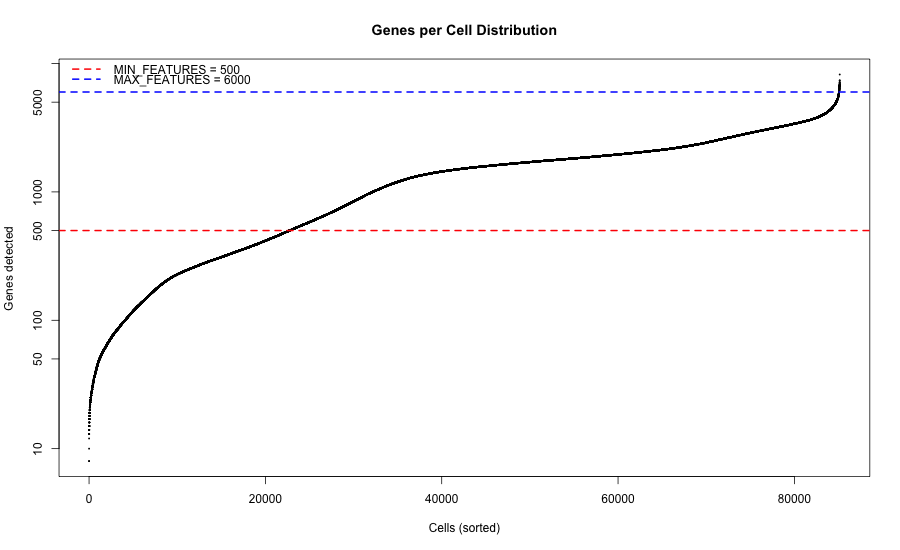
\includegraphics[width=0.85\textwidth]{plots/phase1/phase1_step05_genes_per_cell.png}
\end{center}

\begin{itemize}[nosep]
  \item The left side of the curve (first $\sim$5,000 cells when sorted) drops sharply to
        very low gene counts — these are almost certainly empty droplets with only ambient RNA.
  \item The middle section rises gradually and smoothly — this is the real cell population.
  \item At the very far right, a small sharp uptick exceeds 6,000 genes — these are likely
        doublets (two cells captured together appear as one unusually gene-rich cell).
  \item \textbf{Conclusion:} the thresholds MIN = 500 and MAX = 6,000 are well-placed.
        The red line sits just above the dropout cliff and the blue line catches the doublet spike.
\end{itemize}

\subsubsection*{Step 7 — Mitochondrial content distribution}

\begin{center}
  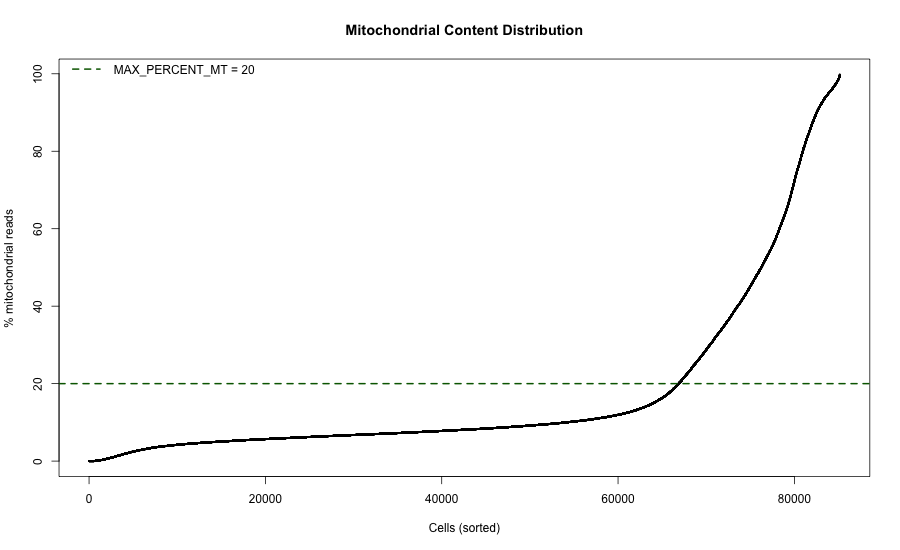
\includegraphics[width=0.85\textwidth]{plots/phase1/phase1_step07_mito_distribution.png}
\end{center}

\begin{itemize}[nosep]
  \item The first $\sim$65,000 cells (sorted) stay flat and low, mostly under 15\% — these look healthy.
  \item From $\sim$65,000 onwards the curve rises sharply and exponentially, reaching 100\%.
  \item This means roughly 20,000 cells ($\sim$25\% of the dataset) have $>$20\% mitochondrial content.
  \item This is an unusually high proportion, suggesting the blood samples contained a lot of
        stressed or damaged cells, which is actually consistent with severe COVID-19.
  \item \textbf{Conclusion:} the 20\% threshold (green dashed line) is a reasonable cutoff.
        It preserves the large flat healthy region and removes the exponential tail.
\end{itemize}

\subsubsection*{Step 8 — Violin and scatter plots}

\begin{center}
  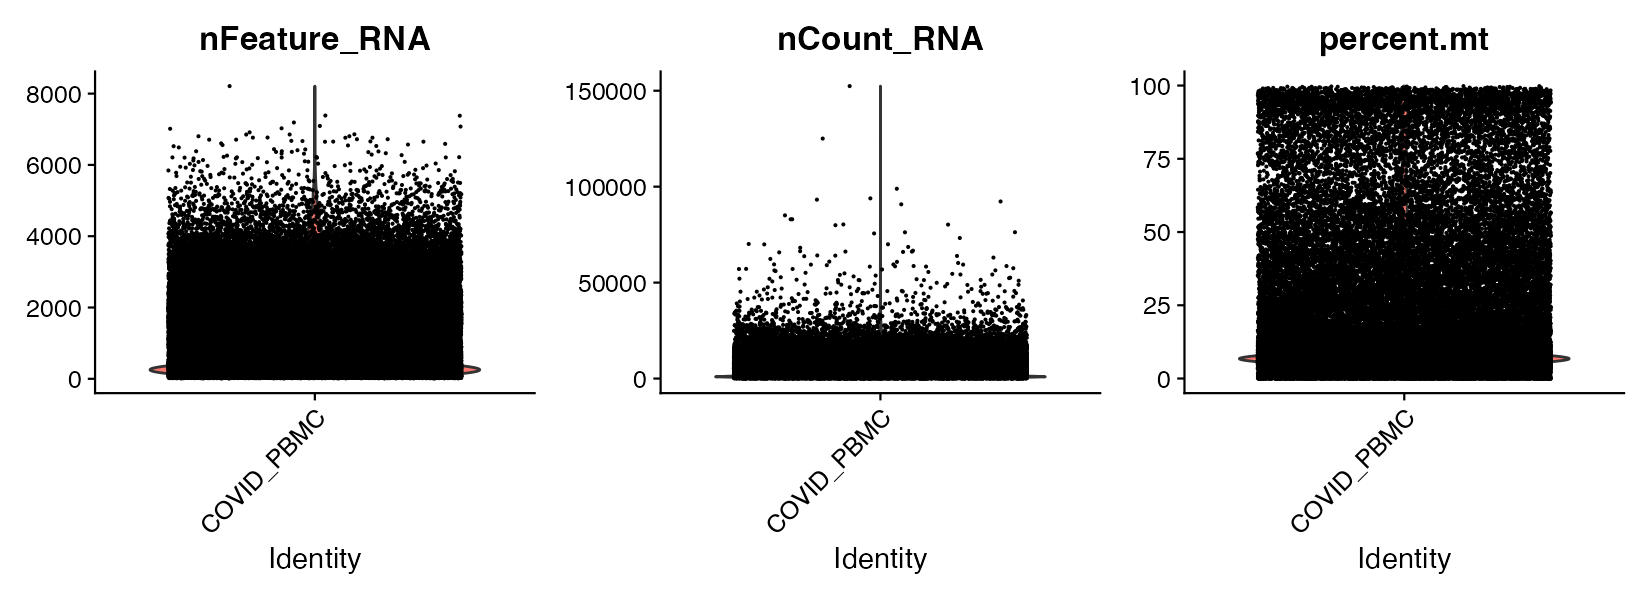
\includegraphics[width=\textwidth]{plots/phase1/phase1_step08_violin_qc_metrics.png}
\end{center}

\begin{center}
  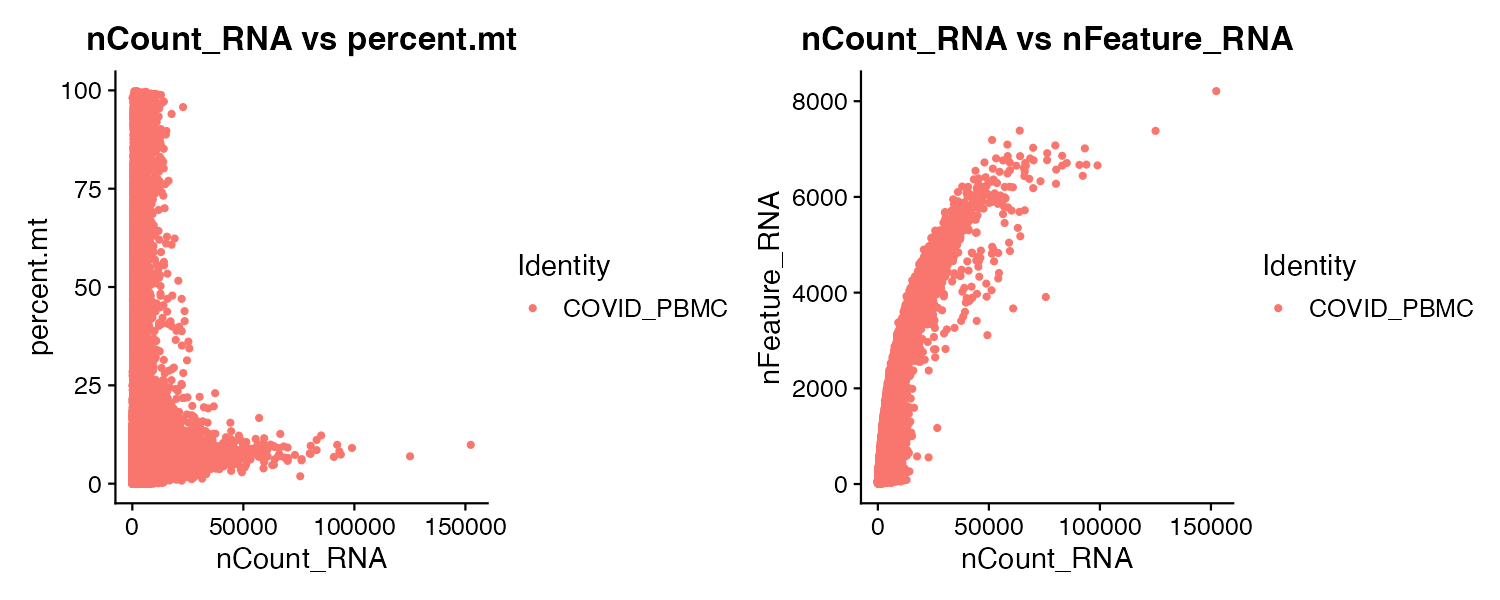
\includegraphics[width=0.95\textwidth]{plots/phase1/phase1_step08_scatter_qc_metrics.png}
\end{center}

\textit{Violin plots (nFeature\_RNA, nCount\_RNA, percent.mt):}
\begin{itemize}[nosep]
  \item \textbf{nFeature\_RNA}: a very dense mass of cells compressed near zero (empty droplets /
        low-quality) with a thinner body of real cells above 500.
        A few outliers reach above 6,000 (doublet candidates).
  \item \textbf{nCount\_RNA}: same pattern — a large low-count mass at the bottom, a real-cell body
        in the middle, and isolated high-count outliers above 40,000–50,000.
  \item \textbf{percent.mt}: extremely wide violin spreading from near 0 to 100\%.
        This confirms the heavy tail of damaged cells seen in step 7.
\end{itemize}

\textit{Scatter plots:}
\begin{itemize}[nosep]
  \item \textbf{nCount\_RNA vs percent.mt} — classic ``L'' shape. Cells with very low counts
        are scattered at all mitochondrial percentages up to 100\% (damaged / dying cells).
        The healthy cells cluster tightly at the bottom with low mito\%.
        This pattern confirms that low count + high mito go together as a double sign of bad quality.
  \item \textbf{nCount\_RNA vs nFeature\_RNA} — tight upward curve confirming the two metrics
        are correlated. A few dots at the top-right (above 6,000 genes, above 100,000 counts)
        are outliers consistent with doublets.
        The non-linear curve (not a straight line) is expected because each extra count
        becomes less likely to represent a new gene the more genes are already detected.
\end{itemize}

\subsection{Filter low-quality cells \small\normalfont\textit{(Steps 9–12)}}
Cells are removed if they fall outside the chosen thresholds:
too few genes (likely empty droplets), too many genes or UMIs (likely doublets),
or too high mitochondrial content (likely dying cells).
The filtered Seurat object is saved for Phase 2.

\textbf{Step 9 — cells flagged per filter:}

\medskip
\noindent
\begin{tabular}{@{}p{4.5cm}p{2cm}p{6cm}@{}}
\toprule
\textbf{Filter} & \textbf{Cells} & \textbf{Likely cause} \\
\midrule
nFeature\_RNA $\leq$ 500  & 22,774 & Empty droplets / ambient RNA \\
nCount\_RNA $\leq$ 1,000  & 13,959 & Low-quality / weak capture \\
percent.mt $\geq$ 20\%    & 18,282 & Damaged or dying cells \\
nFeature\_RNA $\geq$ 6,000 & 77    & Doublet candidates \\
nCount\_RNA $\geq$ 40,000  & 161   & Doublet candidates \\
\bottomrule
\end{tabular}

\medskip
\textbf{Step 10 — filtering outcome:}
\begin{itemize}[nosep]
  \item Cells before: 85,144
  \item Cells after: 55,548
  \item Cells removed: 29,596 (\textbf{34.8\% of the dataset})
\end{itemize}

The largest single source of removed cells was the low-gene filter (22,774 empty droplets),
followed closely by the high-mitochondrial filter (18,282 damaged cells).
Doublets were rare — only 238 cells combined — consistent with a well-run 10X experiment.

\textbf{Step 12 — post-filtering QC summary:}
\begin{itemize}[nosep]
  \item Median nFeature\_RNA: 1,872 genes/cell
  \item Median nCount\_RNA: 5,845 UMIs/cell
  \item Median percent.mt: 7.32\%
\end{itemize}

\subsubsection*{Step 11 — Before vs after filtering}

\begin{center}
  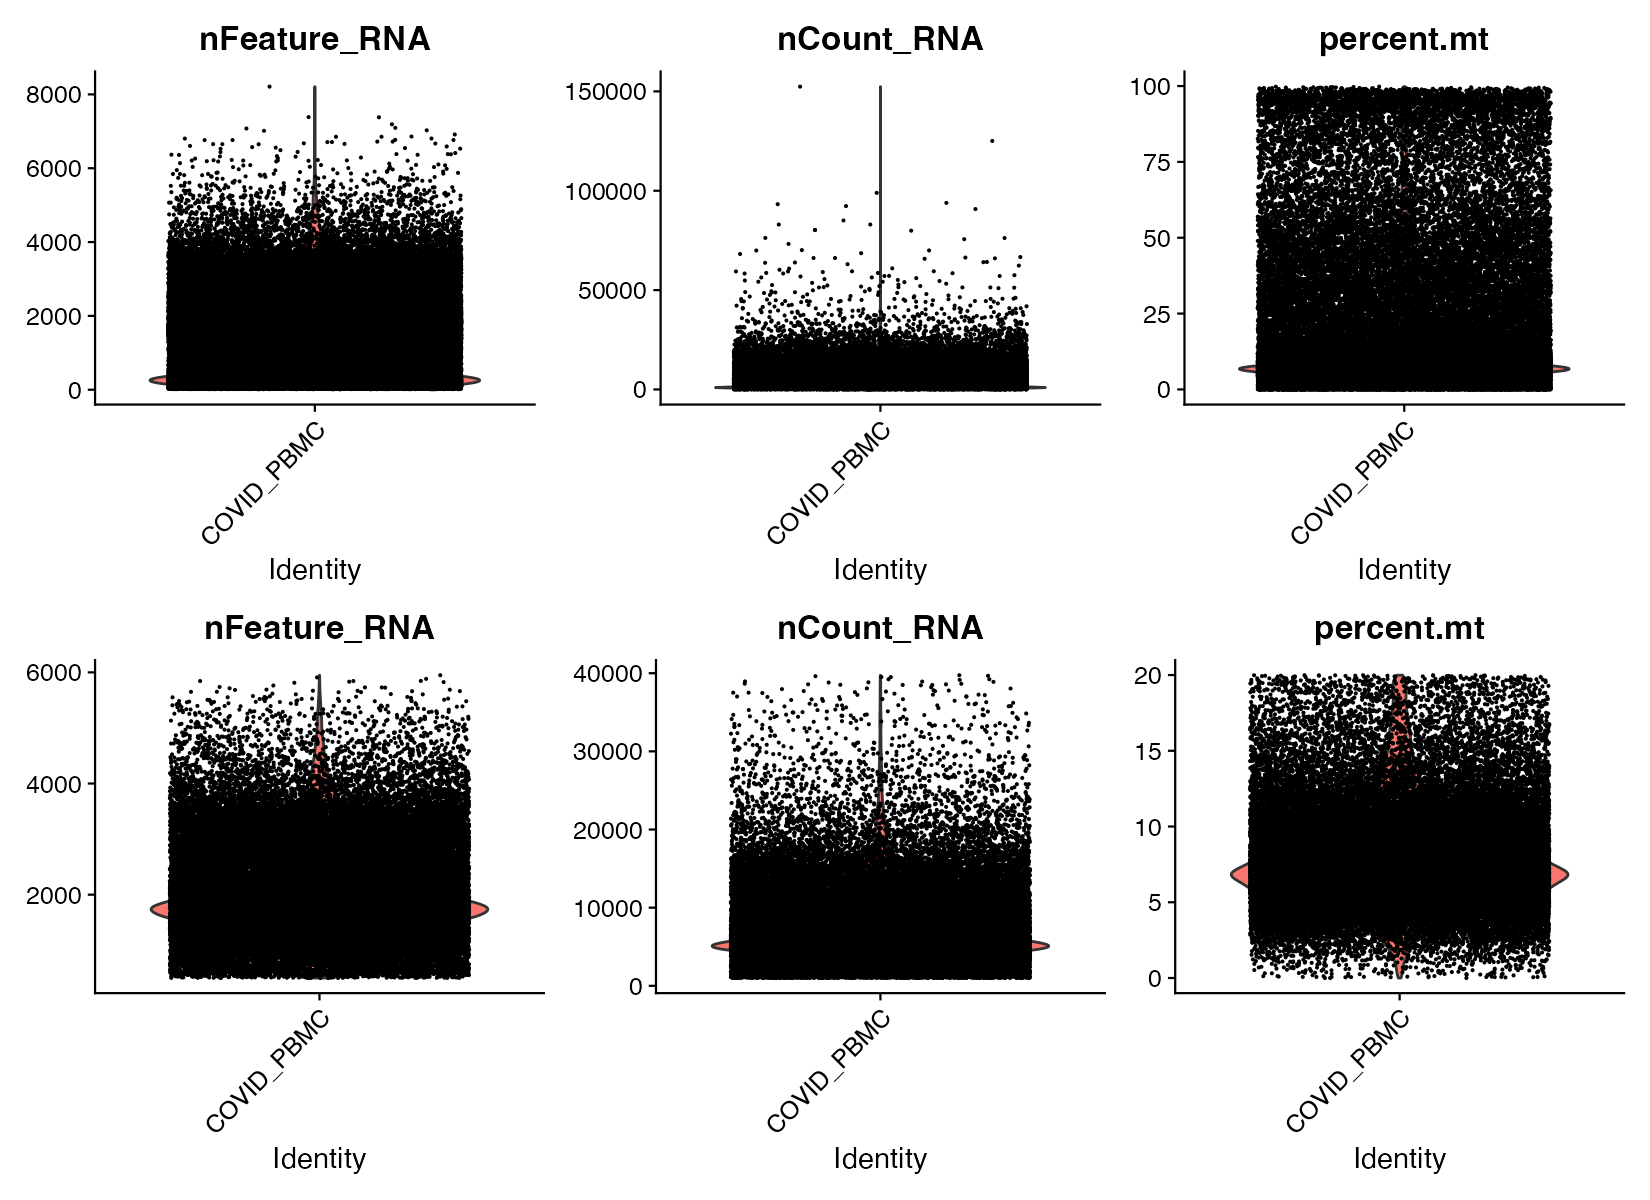
\includegraphics[width=\textwidth]{plots/phase1/phase1_step11_before_after_filtering.png}
\end{center}

\textit{Top row = before filtering. Bottom row = after filtering.}

\begin{itemize}[nosep]
  \item \textbf{nFeature\_RNA}: before, a huge compressed mass sits near zero with a long tail up to
        8,000. After, the distribution is clean and centered around 1,500--2,000 with a tight upper
        bound below 6,000. The noise is gone.
  \item \textbf{nCount\_RNA}: before, the violin is dominated by an enormous low-count mass with a few
        extreme outliers near 150,000. After, the distribution is compact and centered around
        5,000--20,000 with the outliers removed.
  \item \textbf{percent.mt}: the most dramatic change. Before, the violin fills the entire 0--100\%
        range — nearly half the plot. After, it collapses to a tight shape below 20\%, with a
        median of 7.3\%. This confirms that a large portion of the original data was damaged cells.
\end{itemize}

\textbf{Overall conclusion:} the filtering was effective and the thresholds were appropriate.
The retained 55,548 cells represent a clean dataset of real, single, reasonably healthy cells
ready for normalization and downstream analysis.

\subsection{Phase 1 conclusion}

Phase 1 started with a large but noisy dataset and produced a clean, filtered object ready
for biological analysis. The key outcomes are:

\begin{itemize}[nosep]
  \item \textbf{85,144 cells} entered QC; \textbf{55,548 cells} passed (34.8\% removed).
  \item The largest source of removed cells was empty droplets and low-quality captures
        (too few genes or UMIs), which made up the majority of the flagged entries.
  \item A substantial fraction (21.5\%) had excessive mitochondrial content, consistent
        with the blood samples coming from severely ill COVID-19 patients where cell stress
        and damage is expected.
  \item Doublets were rare (0.3\%), confirming the 10X capture was clean.
  \item After filtering, the typical cell has 1,872 detected genes, 5,845 total UMI counts,
        and only 7.3\% mitochondrial RNA — all healthy values.
  \item The filtered Seurat object is saved to \texttt{Data/phase1\_seurat\_filtered.rds}
        and is the input for Phase 2.
\end{itemize}

\textbf{The one important observation for the project:} the unusually high proportion of
damaged cells (18,282 cells with $>$20\% mito) in the raw data is itself a biological
signal. It suggests that the blood samples — collected from COVID-19 patients of varying
severity — contained many stressed or dying immune cells, which aligns with the
hypothesis that severe COVID causes widespread immune cell dysregulation.

\subsubsection*{Things worth mentioning}

\begin{itemize}[nosep]
  \item \textbf{Doublet detection was incomplete.}
        Only 238 cells (0.3\%) were removed by the upper gene/count thresholds.
        The expected doublet rate for 10X experiments is 1–5\%, meaning roughly
        850–4,250 doublets may still be present in the filtered dataset.
        Fixed thresholds are a coarse filter for doublets; a dedicated tool such as
        DoubletFinder would catch more. This is a known limitation worth noting in the
        write-up.

  \item \textbf{The lower-bound threshold (MIN\_FEATURES = 500) could be justified more precisely.}
        The value was chosen visually from the genes-per-cell plot.
        A more rigorous approach is to fit the inflection point of the sorted curve or
        use a MAD-based rule ($< \text{median} - 3 \times \text{MAD}$).
        The chosen value happens to land in a reasonable place, but the reasoning could
        be made more explicit.

  \item \textbf{Post-filtering metrics are still raw counts — not normalized.}
        The medians (1,872 genes / 5,845 UMIs per cell) confirm healthy capture quality,
        but cells cannot yet be compared to each other until normalization in Phase 2
        removes the effect of varying sequencing depth per cell.

  \item \textbf{No per-sample QC was performed.}
        The dataset contains 20 donors across four groups (Severe COVID, Mild COVID,
        Flu, Healthy). Applying QC globally without checking whether any single donor
        contributes disproportionately many low-quality cells can mask sample-level
        issues. This would be worth checking if the downstream clustering shows
        one cluster driven by a single donor.
\end{itemize}

% ─────────────────────────────────────────────
\section{Phase 2 — Normalization and Dimensionality Reduction}
% ─────────────────────────────────────────────

\subsection{Phase 2 overview — the big picture}

\textbf{Phase 1 cleaned the cells. Phase 2 organizes the clean cells so we can start seeing structure. Phase 3 names the groups.}

The shortest possible chain:
\begin{itemize}[nosep]
  \item \textbf{Phase 1} = remove bad cells
  \item \textbf{Phase 2} = organize good cells so structure appears
  \item \textbf{Phase 3} = identify and name the groups
\end{itemize}

After filtering, we have a matrix of 55,548 cells $\times$ 23,335 genes.
Phase 2 makes those numbers comparable, removes noise, and compresses the data
into a form we can visualize. It does this in four steps:

\begin{enumerate}[nosep]
  \item \textbf{Normalize} — make counts fair to compare across cells (see Background)
  \item \textbf{Select variable genes} — keep only the most informative genes (see Background)
  \item \textbf{Scale and regress} — put genes on a common scale, remove confounders (see Background)
  \item \textbf{PCA → UMAP/t-SNE} — compress from 3,000 genes → 20 PCs → 2D map (see Background)
\end{enumerate}

At the end, we have a 2D picture where similar cells sit near each other.
Phase 3 then asks: \textit{what are these groups of cells actually called?}

\subsection{Normalize and identify variable features \small\normalfont\textit{(Step 4)}}
Raw counts are log-normalized (divided by total cell counts, scaled to 10{,}000,
then log-transformed) so that cells of different sequencing depths are comparable.
The 3{,}000 most variable genes are selected to focus on biologically informative
signal.
Finally, the data are scaled and the mitochondrial percentage is regressed out
to remove its confounding effect.

\textit{Note: SCTransform was attempted but fails with an out-of-memory error on this dataset size. LogNormalize is used instead and is well-established in the literature.}

\textbf{Results:}
\begin{itemize}[nosep]
  \item Object loaded: 55,548 cells, 23,335 genes — matches the Phase 1 output exactly.
  \item \texttt{NormalizeData}: log-normalization completed on all 55,548 cells with no warnings, confirming that every cell has at least some RNA counts (no zero-total cells slipped through Phase 1 filtering).
  \item \texttt{FindVariableFeatures}: selected 3,000 most variable genes out of 23,335 using the VST method. These genes capture the biological differences between cell types while discarding housekeeping genes that are uniformly expressed everywhere.
  \item \texttt{ScaleData}: regressed out \texttt{percent.mt} from all 3,000 variable genes, then centered and scaled. This removes the confounding effect of mitochondrial content from PCA — any remaining variation driven by cell stress rather than cell identity is subtracted out before dimensionality reduction.
\end{itemize}

\textbf{What was accomplished:} the count matrix now exists in three forms inside the Seurat object — raw counts, log-normalized values, and scaled/regressed values. PCA will use the scaled layer. All three are stored and none are overwritten.

\subsection{PCA and choosing the number of components \small\normalfont\textit{(Steps 5–6)}}
PCA is run on the 3,000 variable genes selected in Step 4.
We inspect the PC loadings, PC heatmaps, and the elbow plot to choose how many
PCs to carry into UMAP, t-SNE, and clustering.

\subsubsection*{Step 5a — PC loadings (which genes drive each PC?)}

\begin{center}
  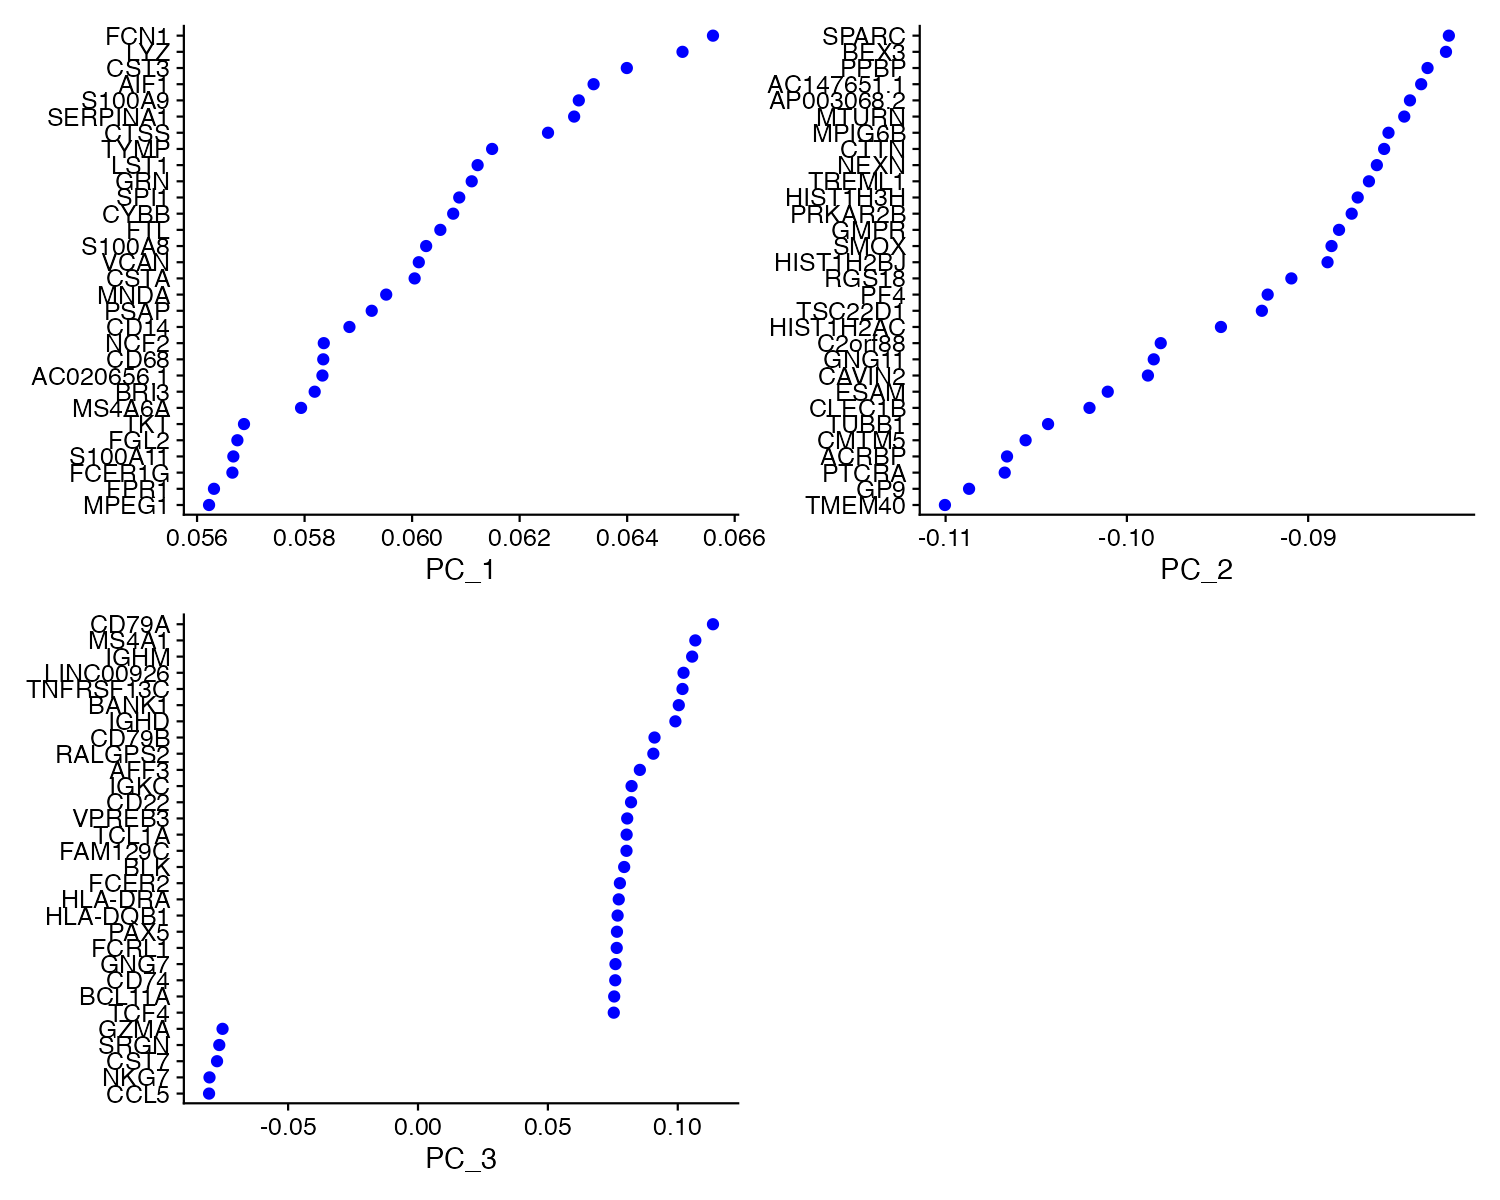
\includegraphics[width=\textwidth]{plots/phase2/phase2_step05a_pc_loadings.png}
\end{center}

The loadings show the genes that contribute most to each of the first three PCs.
The biological interpretation is immediately clear:

\begin{itemize}[nosep]
  \item \textbf{PC1 — monocyte identity.}
        The top positive genes are \textit{FCN1}, \textit{LYZ}, \textit{CST3},
        \textit{S100A9}, \textit{SERPINA1} — all canonical markers of
        classical monocytes. PC1 separates the large monocyte population from
        all other cell types. This is the strongest PC (std $\approx$ 14) by far.

  \item \textbf{PC2 — platelet / megakaryocyte signal.}
        The top negative genes include \textit{CLEC1B}, \textit{TUBB1},
        \textit{MPIG6B}, and several histone genes (\textit{HIST1H3E},
        \textit{HIST1H2AC}) — all known platelet and megakaryocyte markers.
        PC2 captures platelet-associated cells or platelet contamination in
        the PBMC preparation.

  \item \textbf{PC3 — B cells vs NK/T cells.}
        The top positive genes are \textit{CD79A}, \textit{MS4A1}, \textit{IGHM}
        — B cell markers. The most negative genes are \textit{NKG7}, \textit{CCL5},
        \textit{GZMA}, \textit{GZMK} — cytotoxic T and NK cell markers.
        PC3 separates the lymphoid compartment along the B cell / cytotoxic axis.
\end{itemize}

The fact that the first three PCs each capture a distinct and biologically meaningful
cell-type axis confirms that the normalization and feature selection in Step 4 worked
correctly. PCA is finding real biology, not technical noise.

\subsubsection*{Step 5b — PC heatmaps (how clean is the signal in each PC?)}

\begin{center}
  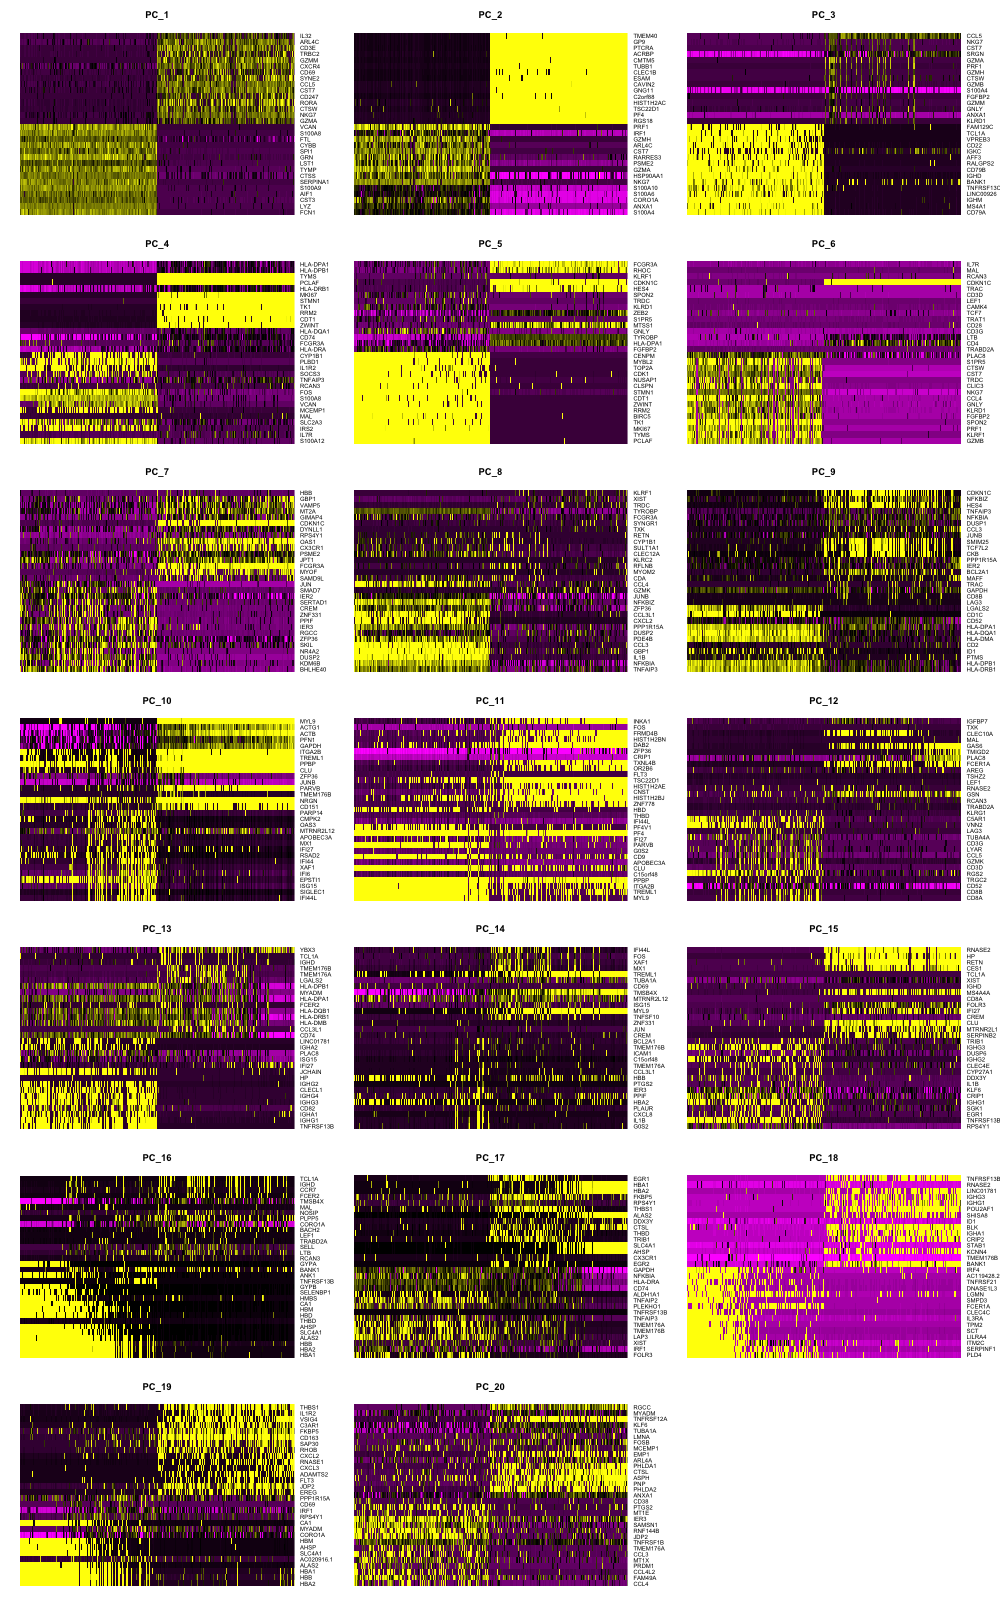
\includegraphics[width=\textwidth]{plots/phase2/phase2_step05b_pc_heatmaps.png}
\end{center}

Each panel shows 500 cells (250 with the highest and 250 with the lowest score for
that PC). Yellow = high expression, purple = low. A clean PC shows two sharply
contrasting blocks; a noisy PC shows a patchy, mixed pattern.

\begin{itemize}[nosep]
  \item \textbf{PC1–3}: Extremely clean. Two solid blocks with almost no mixing.
        These PCs are capturing strong, consistent cell-type differences.
  \item \textbf{PC4–10}: Clear structure, slightly more heterogeneous within blocks.
        These PCs are capturing real but subtler differences (sub-populations,
        activation states).
  \item \textbf{PC11–15}: More mixed. Structure is still detectable — this is not
        pure noise — but the within-block variation is growing.
  \item \textbf{PC16–20}: Noticeably patchier. Some PCs show faint structure;
        others are mostly mixed. These are at the boundary between meaningful signal
        and noise.
\end{itemize}

The heatmaps support using 15–20 PCs. Going beyond 20 would start to include PCs
that are predominantly noise.

\subsubsection*{Step 6 — Elbow plot (how many PCs to use?)}

\begin{center}
  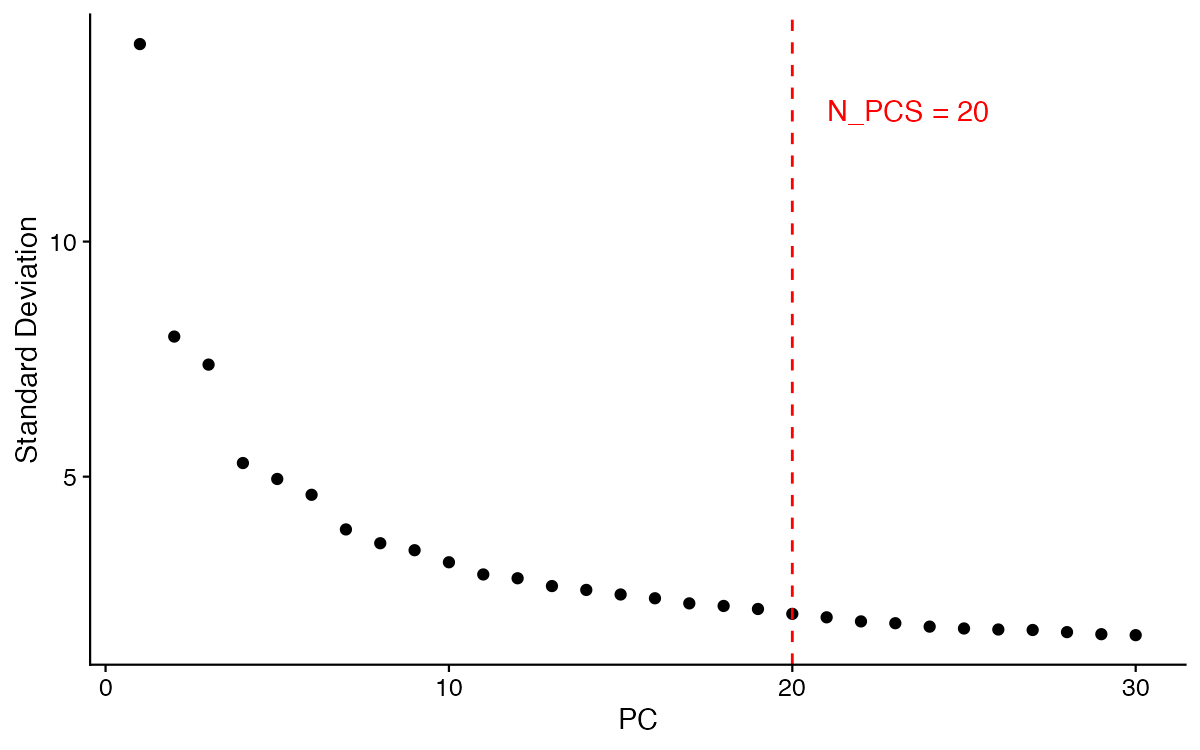
\includegraphics[width=0.85\textwidth]{plots/phase2/phase2_step06_elbow_plot.png}
\end{center}

The elbow plot shows the standard deviation of each PC in decreasing order.

\begin{itemize}[nosep]
  \item \textbf{PC1} dominates with std $\approx$ 14 — the monocyte signal is enormous.
  \item \textbf{PC2–3}: std $\approx$ 8 and 7 — still strongly informative.
  \item \textbf{PC4–10}: Gradual decline from $\sim$5 to $\sim$2.5.
  \item \textbf{PC10–20}: Slow, nearly linear decline from $\sim$2.5 to $\sim$1.5.
        The curve is visibly flattening in this range.
  \item \textbf{PC20–30}: Essentially flat at $\sim$1–1.5 — this is the noise floor.
\end{itemize}

The elbow in this dataset is not a single sharp bend but a gradual transition,
which is typical for complex datasets with many cell types and sub-states.
The clearest plateau begins around PC\,20, which is where the dashed cutoff line is placed.

\textbf{Decision: N\_PCS = 20.}
This is well-justified by all three plots together:
the heatmaps show meaningful structure through PC\,20,
the loadings show biologically interpretable axes in the early PCs,
and the elbow plot is flat after PC\,20.
Using 15 would likely lose some subtle subpopulation structure visible in PC\,16–20;
using 25 would add mostly noise.

\subsection{UMAP and t-SNE embeddings \small\normalfont\textit{(Steps 7–9)}}
UMAP and t-SNE are computed from the first 20 PCA dimensions to project
55,548 cells into a 2-D layout for visualisation.

\textit{Note: Seurat's default UMAP backend switched from Python (umap-learn) to
the R-native UWOT library with cosine metric. This is expected behaviour in
Seurat 5 and produces comparable results.}

\subsubsection*{Step 7 — UMAP}

\begin{center}
  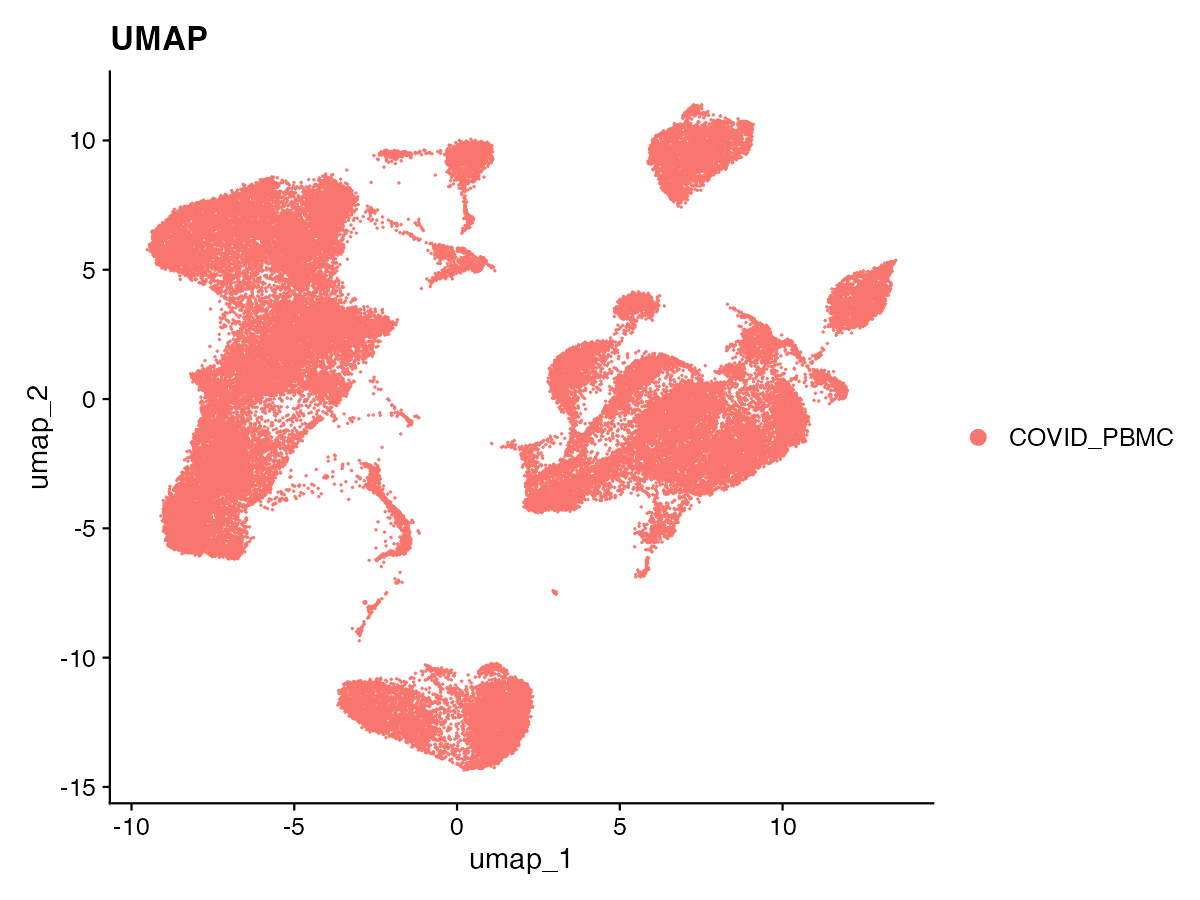
\includegraphics[width=0.85\textwidth]{plots/phase2/phase2_step07_umap.png}
\end{center}

The UMAP shows \textbf{clear, well-separated clusters} with distinct gaps between
groups — a strong sign that the normalization and PCA captured real biological
structure. Key observations:

\begin{itemize}[nosep]
  \item \textbf{Large left mass} — the biggest continuous region in the plot.
        Given that PC1 was dominated by monocyte markers (FCN1, LYZ, S100A9),
        this is almost certainly the monocyte/myeloid compartment. Its size is
        consistent with monocytes being the most abundant cell type in COVID PBMC samples.
  \item \textbf{Upper-right islands} — two well-separated compact blobs above and
        to the right of center. Likely T cell subsets (CD4$^+$ and CD8$^+$), separated
        by their distinct transcriptional programs.
  \item \textbf{Lower-right leaf shape} — a dense, compact, somewhat isolated cluster.
        Candidate: B cells or NK cells.
  \item \textbf{Bottom island} — a tight, clearly separated cluster at the bottom.
        Likely platelets or a rare cell type (consistent with the PC2 platelet signal).
  \item \textbf{Small satellite blobs} (e.g.\ top-center) — could be dendritic cells,
        plasma cells, or other rare populations.
\end{itemize}

\textbf{Important caveat:} at this stage the cells are all coloured the same (no cluster
labels yet). The visual groupings above are inferences from the PCA biology. Phase 3 will
assign cell-type labels and confirm or revise these interpretations.

\subsubsection*{Step 8 — t-SNE}

\begin{center}
  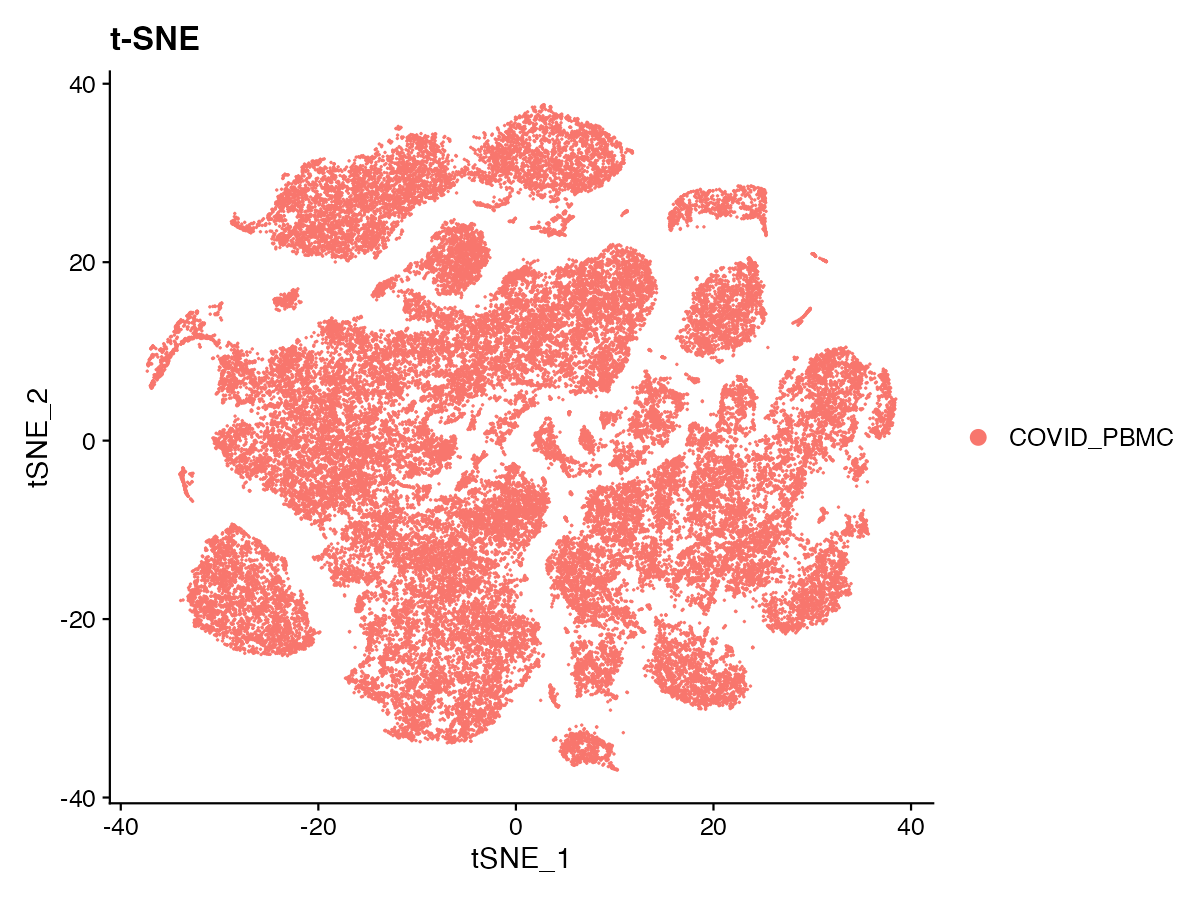
\includegraphics[width=0.85\textwidth]{plots/phase2/phase2_step08_tsne.png}
\end{center}

The t-SNE shows the same broad population structure as UMAP but with a different layout
style: more scattered, more fragmented between the clusters, and with more internal
sub-structure visible within each major group. The same large monocyte mass, separated
lymphoid blobs, and isolated small populations are all present.

\subsubsection*{Step 9 — UMAP vs t-SNE comparison}

\begin{center}
  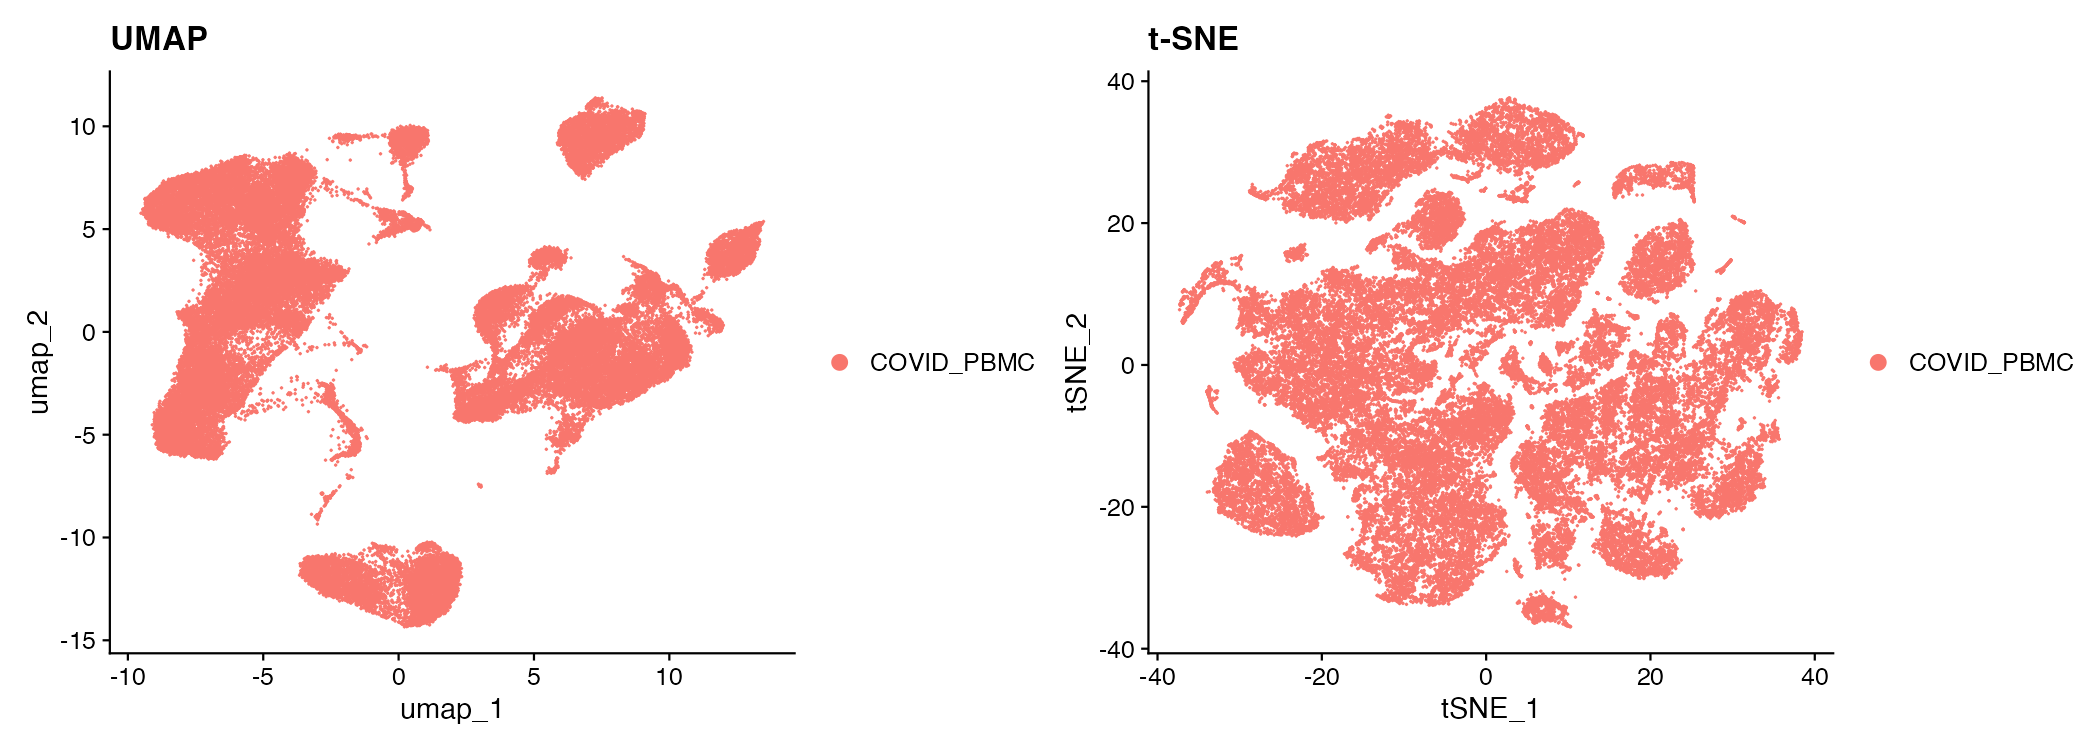
\includegraphics[width=\textwidth]{plots/phase2/phase2_step09_umap_vs_tsne.png}
\end{center}

\begin{itemize}[nosep]
  \item Both embeddings agree on the main story: the dataset contains several clearly
        distinct populations with real gaps between them.
  \item \textbf{UMAP} produces more compact, better-defined cluster shapes and preserves
        more of the global structure (relative cluster positions are more meaningful).
  \item \textbf{t-SNE} spreads the clusters out more and exaggerates within-cluster
        distances, which sometimes reveals sub-structure but also risks over-fragmentation.
  \item For this project, UMAP is used as the primary visualisation going forward.
        t-SNE is kept as a cross-check.
\end{itemize}

\textbf{Overall conclusion of Phase 2:}
The normalization, PCA, and embedding pipeline produced a high-quality representation
of the dataset. The 20-PC cutoff was appropriate, and both UMAP and t-SNE clearly
separate the major PBMC cell types. The data is ready for clustering and annotation
in Phase 3. The processed object is saved to \texttt{Data/phase2\_seurat\_processed.rds}.

% ─────────────────────────────────────────────
\section{Phase 3 — Clustering and Cell-Type Annotation}
% ─────────────────────────────────────────────

\subsection{Phase 3 overview — the big picture}

\textbf{Phase 1 cleaned the cells. Phase 2 organized them so structure appeared. Phase 3 names the groups.}

At the end of Phase 2 we had a UMAP with clear visual blobs but no labels — we could
\textit{see} distinct populations but had no idea what cell types they were.
Phase 3 answers that question in two independent ways:

\begin{enumerate}[nosep]
  \item \textbf{Graph-based clustering} — the algorithm finds groups by looking at which
        cells are nearest neighbours in PCA space, without using any prior biology.
        This gives each cell a cluster number (0, 1, 2, \ldots).
  \item \textbf{Biological annotation} — we look at known marker genes and an automated
        reference-based tool (SingleR) to map cluster numbers to cell-type names.
\end{enumerate}

Using two independent approaches and checking that they agree is what gives the
annotation credibility. Both approaches use the same 20-PC embedding from Phase 2.

\subsection{Graph-based clustering \small\normalfont\textit{(Steps 4–7)}}

A shared-nearest-neighbour (SNN) graph is built from the first 20 PCA dimensions with
\texttt{FindNeighbors()}. Clusters are then detected with the Louvain algorithm via
\texttt{FindClusters()} at five resolutions. Higher resolution = more clusters (the
algorithm cuts the graph more finely); lower resolution = fewer, broader clusters.
The resolution is a free parameter that requires inspection to set correctly.

\subsubsection*{Step 5 — Resolution sweep}

\texttt{FindClusters()} was run at resolutions 0.1, 0.3, 0.5, 0.8, and 1.0.
The resulting cluster counts are:

\begin{center}
\begin{tabular}{cc}
\hline
\textbf{Resolution} & \textbf{Number of clusters} \\
\hline
0.1 & 12 \\
0.3 & 19 \\
0.5 & 23 \\
0.8 & 35 \\
1.0 & 34 \\
\hline
\end{tabular}
\end{center}

The most diagnostic number in this table is the \textbf{drop from 35 to 34} when going from
resolution 0.8 to 1.0. Normally, increasing resolution should add more clusters —
the Louvain algorithm keeps cutting the graph more finely. When the count goes
\textit{down}, it means the algorithm is no longer finding stable structure; it is
splitting real clusters into fragments and then re-merging some of them differently
on each run. This is the textbook sign of \textbf{over-splitting instability}, and
it means $\text{res} \geq 0.8$ should not be used.

\textbf{Resolution 0.1} (12 clusters) is too coarse for the opposite reason: the PBMC
dataset contains more than 12 biologically distinct populations. As the UMAP will show,
the entire myeloid compartment collapses into 2--3 undifferentiated blobs at this resolution.

This leaves \textbf{resolution 0.3–0.5} as the biologically sensible range.

\subsubsection*{Step 6 — Resolution comparison UMAP grid}

\begin{center}
  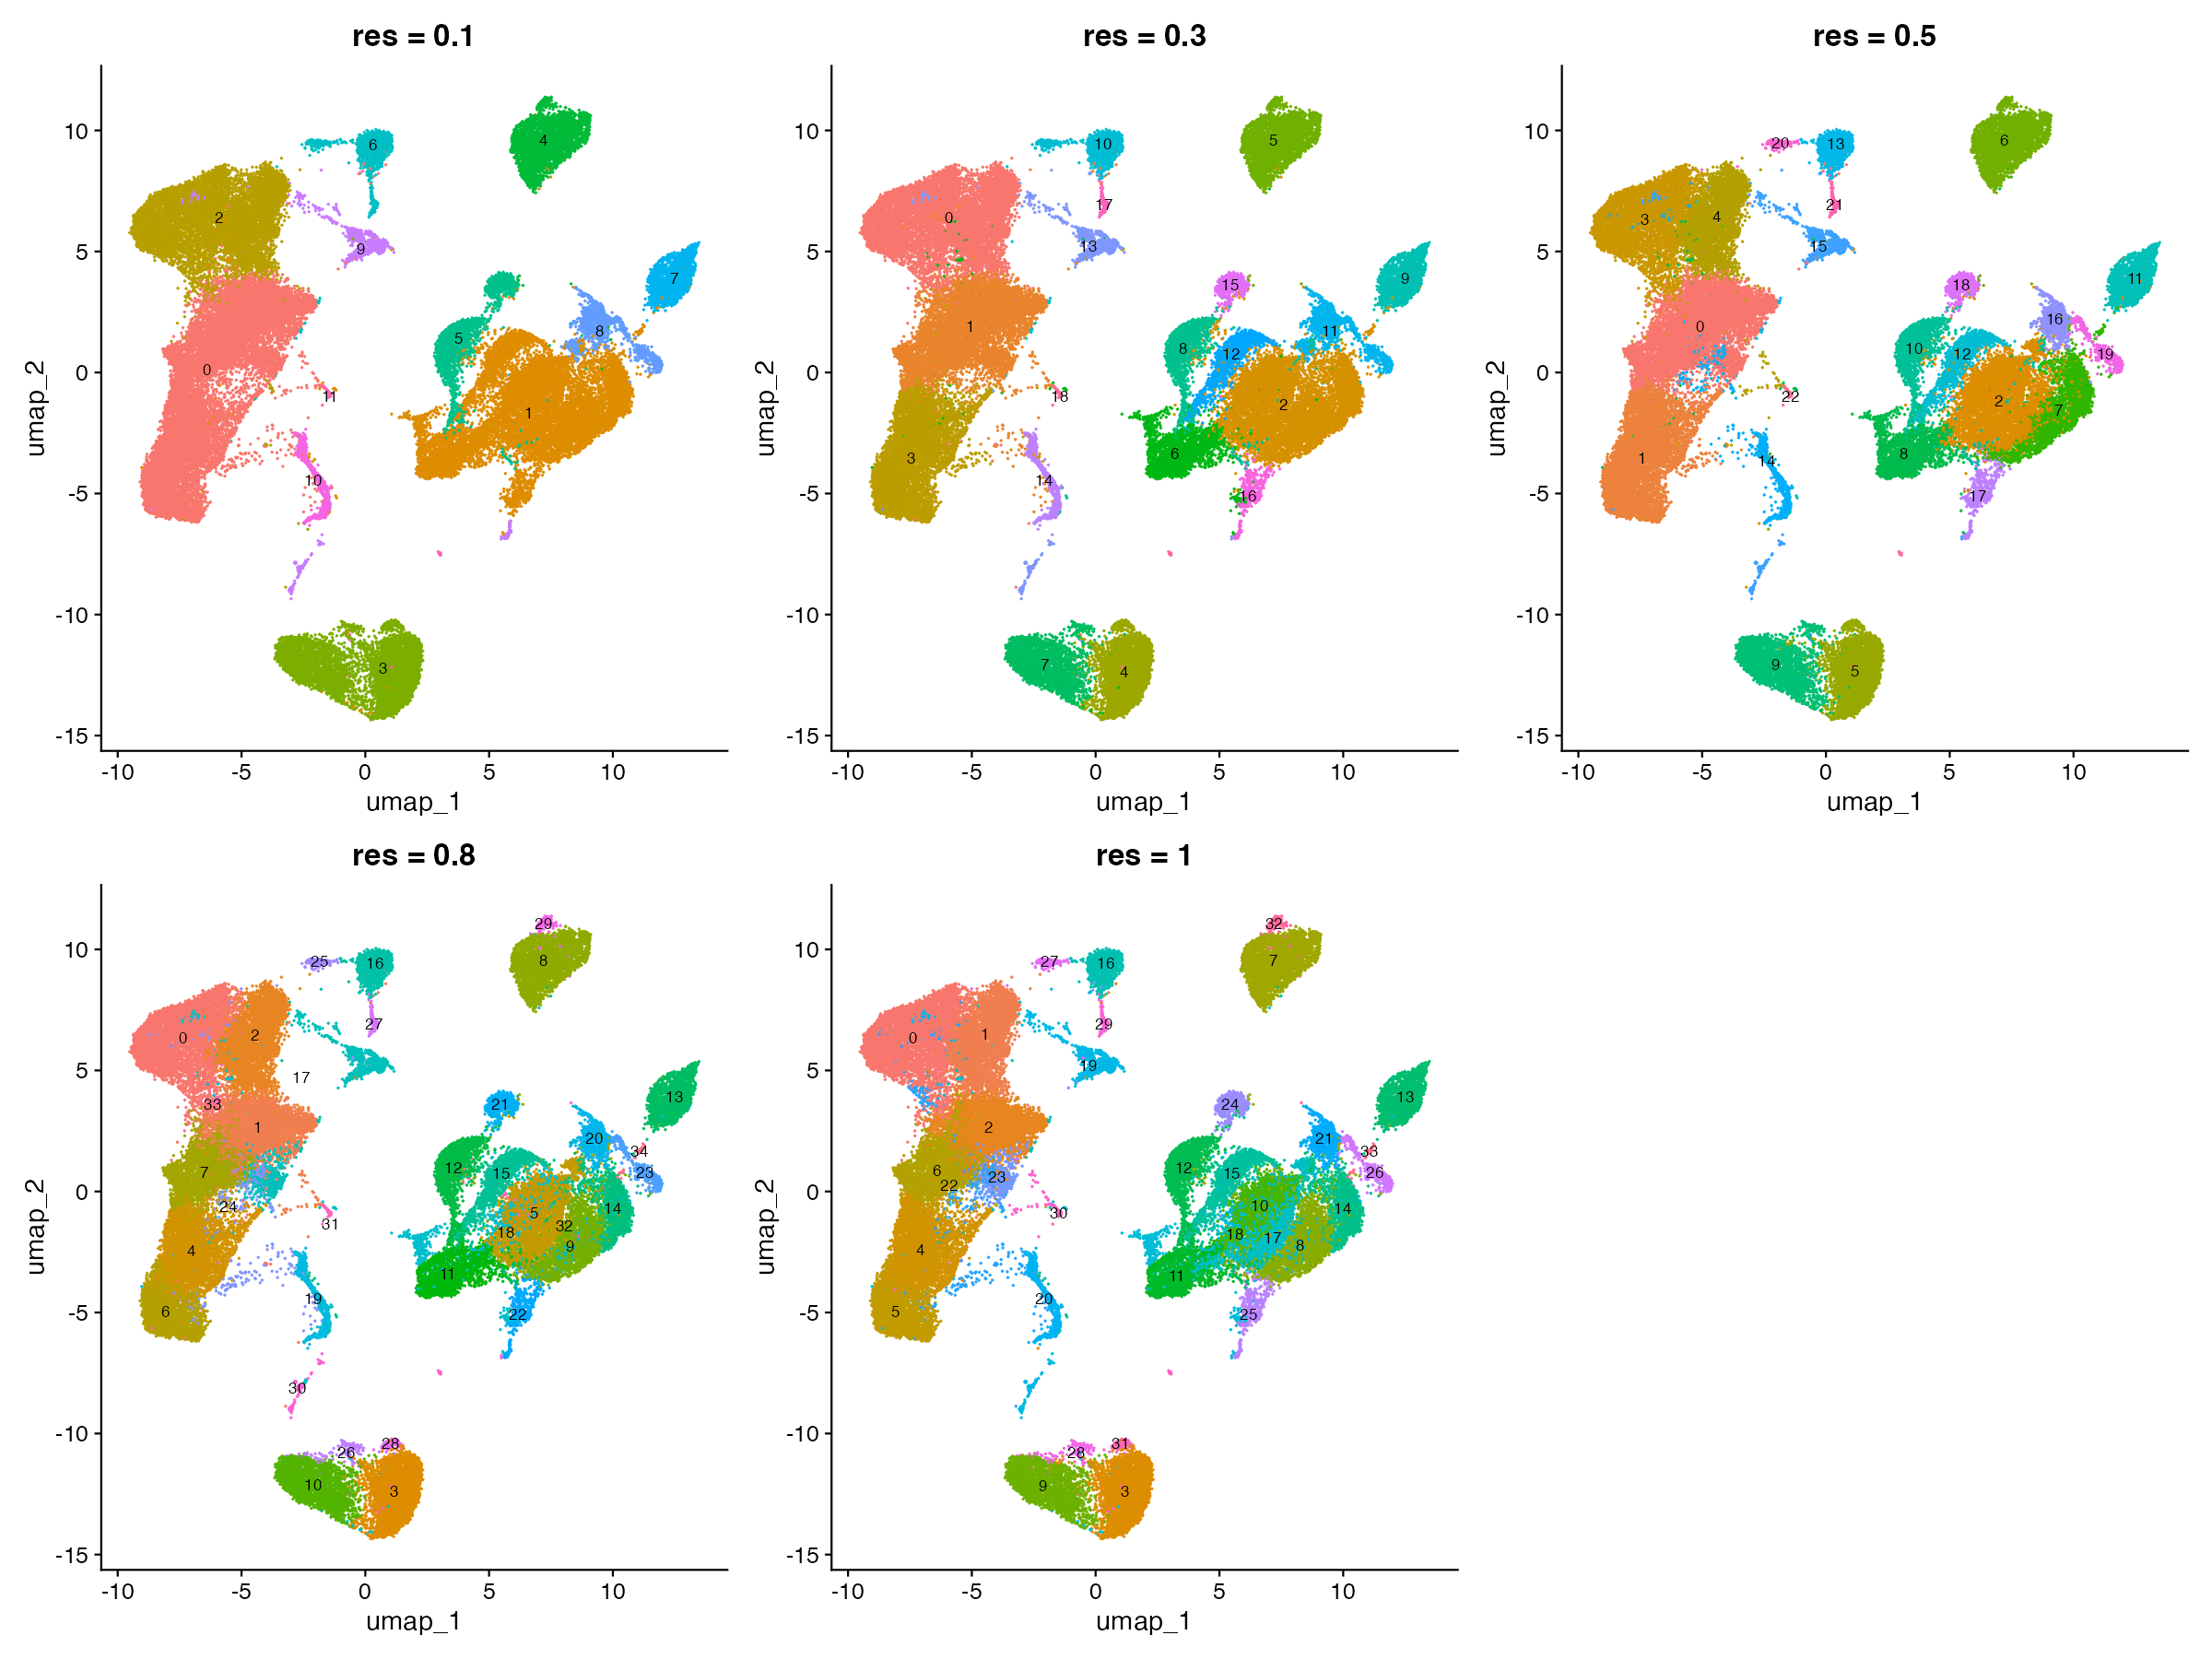
\includegraphics[width=\textwidth]{plots/phase3/phase3_step06_resolutions_comparison.png}
\end{center}

The grid confirms the numerical analysis:

\begin{itemize}[nosep]
  \item \textbf{res = 0.1 (12 clusters):} The large left-side myeloid continent
        is one undifferentiated blob. Multiple biologically distinct monocyte
        subpopulations and the dendritic cell islands are collapsed together.
        Too coarse.

  \item \textbf{res = 0.3 (19 clusters):} Real structure emerges. The major
        compartments (myeloid, T/NK lymphoid, B cell, isolated rare populations)
        separate cleanly. Some sub-populations that are visually distinct may
        still be merged.

  \item \textbf{res = 0.5 (23 clusters):} Clean boundaries throughout. Small
        satellite clusters (the top-centre island, the far-right edge populations)
        are recovered as their own clusters without fragmenting the large continuous
        regions. This is the best-balanced resolution.

  \item \textbf{res = 0.8 (35 clusters):} The right-side T/NK mass begins to
        fragment into confetti — small chips that do not correspond to visually
        distinct regions of the UMAP. Artefactual micro-clusters appear in
        transition zones between major populations.

  \item \textbf{res = 1.0 (34 clusters):} The fragmentation continues and the
        instability (35 $\to$ 34 cluster drop) becomes visible as irregular
        boundary changes with no new biological meaning.
\end{itemize}

\textbf{Decision: FINAL\_RES = 0.5.}
Resolution 0.5 gives 23 clusters that match every visually distinct region in the
UMAP without over-fragmenting the continuous T/NK mass.
This is also the Seurat default, which reflects community consensus on the typical
number of cell types recoverable from PBMC datasets.

\subsubsection*{Step 7a — Final clustering UMAP}

\begin{center}
  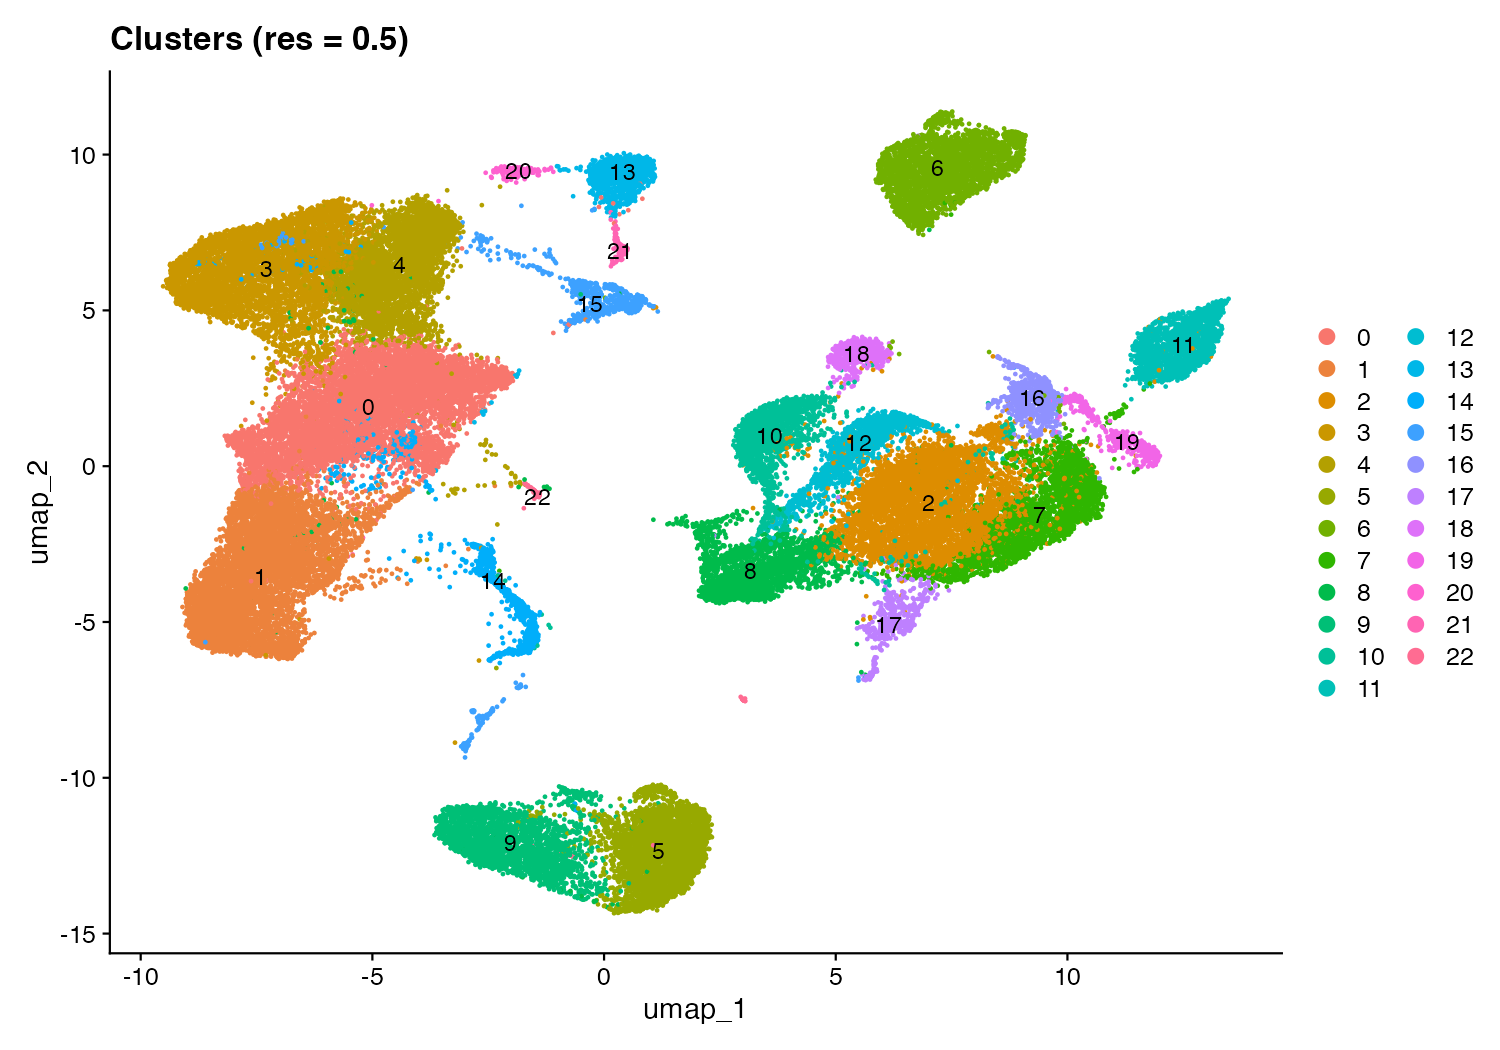
\includegraphics[width=0.9\textwidth]{plots/phase3/phase3_step07a_umap_clusters_final.png}
\end{center}

The UMAP coloured by final clusters (res = 0.5) shows two major continents and
several smaller isolated islands. The topology is already interpretable from the
PCA biology alone (before any marker genes are consulted):

\begin{itemize}[nosep]
  \item \textbf{Left continent (clusters 0, 1, 3, 4) — myeloid compartment.}
        These are the largest, densest clusters. PC1 in Phase 2 was entirely
        dominated by monocyte markers (\textit{FCN1, LYZ, S100A9, CST3}) and
        this continent corresponds to that strong signal. The sub-clusters within
        it likely separate CD14$^+$ classical monocytes from CD16$^+$/non-classical
        monocytes and inflammatory monocyte sub-states. Monocyte expansion is
        a well-documented feature of severe COVID-19.

  \item \textbf{Top-centre isolated group (clusters 13, 15, 20, 21) — rare
        myeloid/lymphoid populations.}
        A small, tightly isolated group of clusters sitting above and to the right
        of the main myeloid mass. The topological isolation from both major
        continents, combined with their small size, is consistent with
        \textbf{plasmacytoid dendritic cells (pDC)} or other rare interferon-producing
        populations, which are known to be transcriptionally very distinct.
        Cluster 22 (between left and right continents, small) may represent
        conventional dendritic cells (cDC1/cDC2), which sit transcriptionally
        between monocytes and lymphocytes.

  \item \textbf{Far right isolated island (cluster 6) — likely NK cells.}
        A compact, completely detached green blob at the far top-right. Complete
        topological isolation from the rest of the lymphoid right continent is
        the characteristic shape of \textbf{NK cells} (Natural Killer cells),
        which have a very distinct transcriptional profile from T cells despite
        occupying adjacent UMAP space in less resolved datasets.

  \item \textbf{Right continent (clusters 2, 7, 8, 10, 11, 12, 16, 18, 19) —
        lymphoid compartment.}
        The broad right-side mass is the T cell and NK compartment.
        Its internal structure likely reflects CD4$^+$ helper T cells, CD8$^+$
        cytotoxic T cells, regulatory T cells (Tregs), and memory vs.\ effector
        sub-states. PC3 in Phase 2 separated NK/CTL genes from B cell genes,
        placing this compartment at the cytotoxic end of that axis.

  \item \textbf{Bottom isolated island (clusters 5, 9) — platelets.}
        The most distinctly isolated cluster: completely detached, sitting at
        the bottom of the UMAP, with a characteristic two-blob shape. PC2 in
        Phase 2 was dominated by platelet/megakaryocyte markers
        (\textit{CLEC1B, TUBB1, MPIG6B}). Platelets are a common contaminant
        in PBMC preparations and always appear as a completely isolated UMAP
        island due to the near-absence of nuclear transcriptomic signal.
\end{itemize}

\subsubsection*{Step 7b — UMAP vs t-SNE comparison}

\begin{center}
  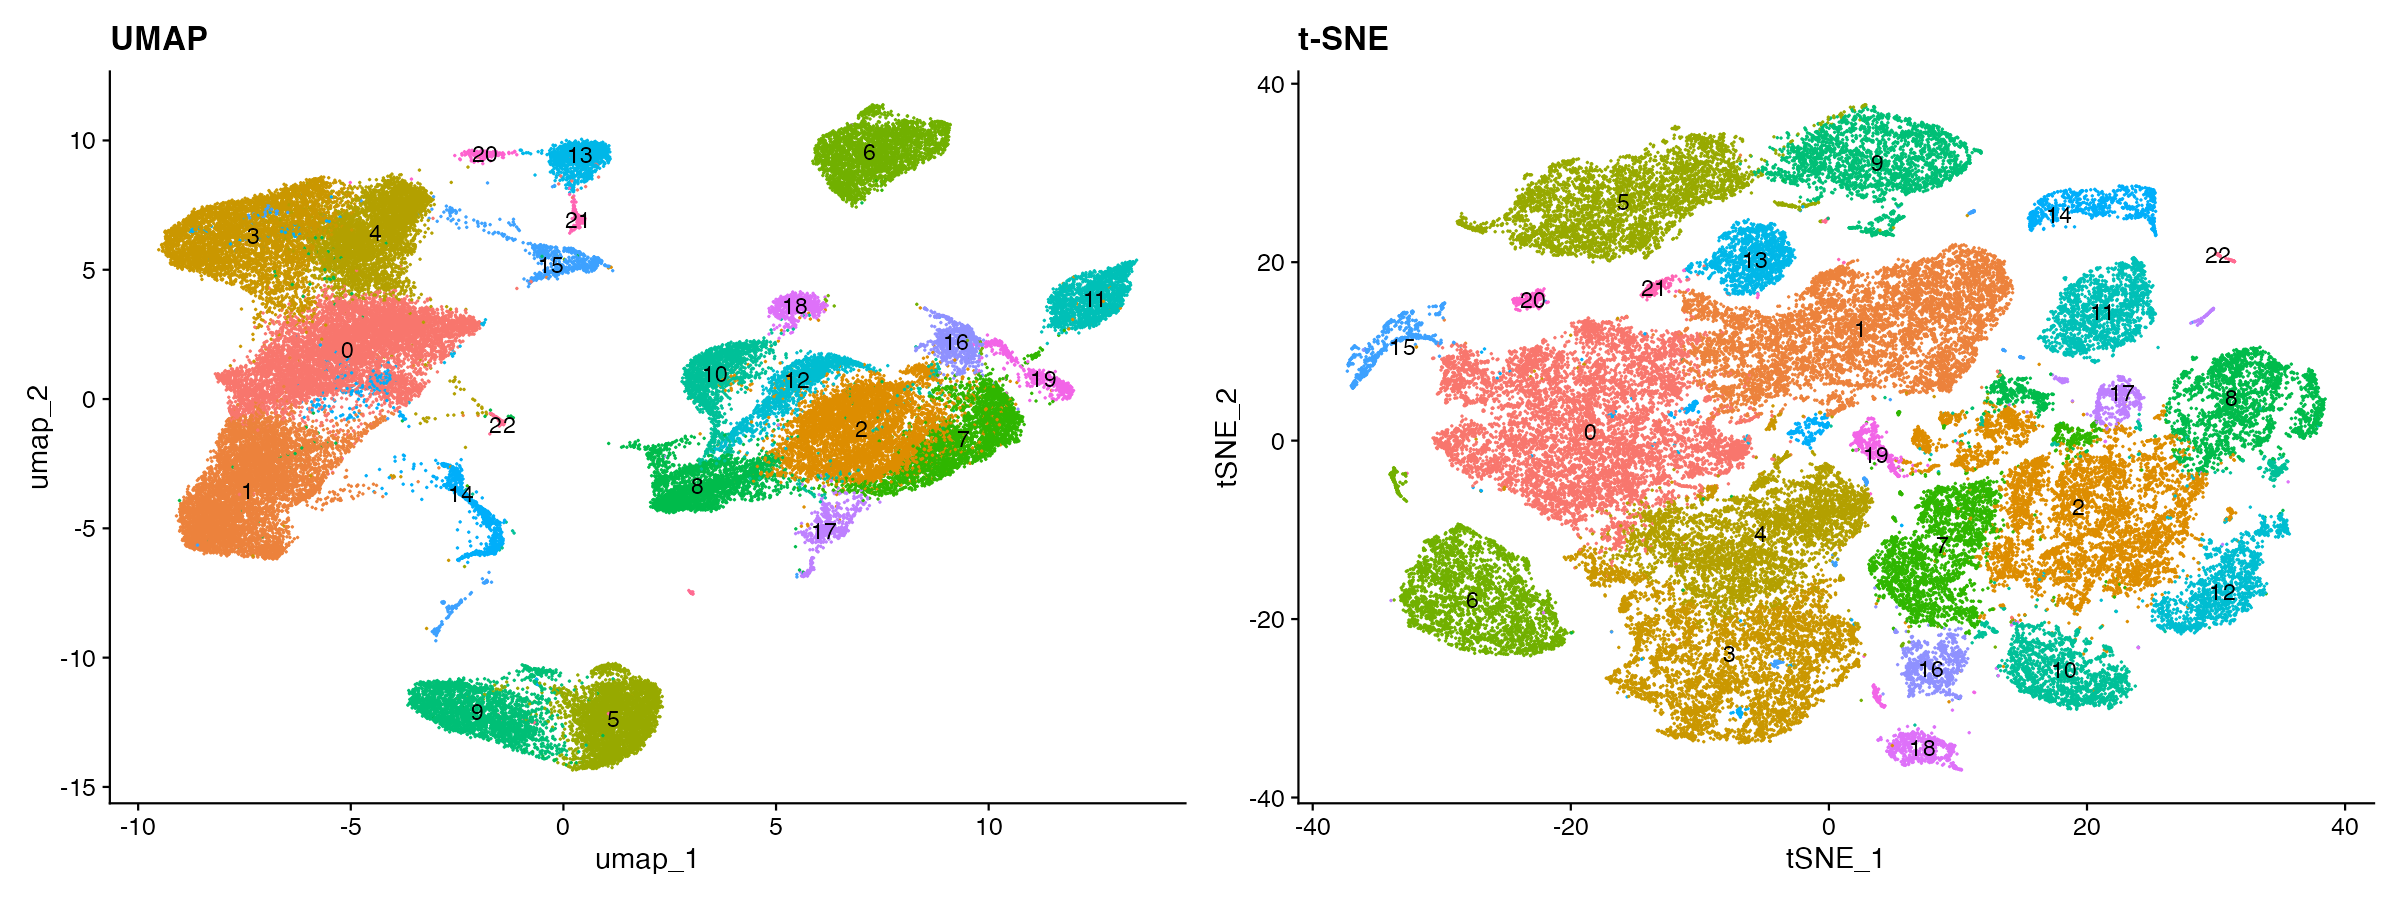
\includegraphics[width=\textwidth]{plots/phase3/phase3_step07b_umap_vs_tsne.png}
\end{center}

Both embeddings show the same cluster structure, which validates that the 23 clusters
are robust features of the data and not artefacts of one particular algorithm.

\begin{itemize}[nosep]
  \item \textbf{Agreement:} All major topological features — the myeloid left continent,
        the lymphoid right continent, the isolated bottom island, and the small
        top-centre group — are present in both plots.
  \item \textbf{UMAP advantage:} Global distances are more meaningful. The clear
        spatial separation between myeloid and lymphoid continents is more
        pronounced, and cluster shapes are more compact and easier to label.
  \item \textbf{t-SNE advantage:} The right-side T/NK mass is spread out more,
        making the internal sub-structure of the lymphoid compartment slightly
        easier to see at this stage. In t-SNE, clusters 6, 11, and 16 are pulled
        further apart from the main T cell mass.
  \item \textbf{Choice:} UMAP is used as the primary visualization going forward.
        t-SNE is kept as a cross-check and confirmation.
\end{itemize}

\subsection{Cell-type annotation \small\normalfont\textit{(Steps 8–9)}}

Two completely independent approaches are used to annotate the 23 clusters.
If both agree, the label is credible. Where they disagree, it indicates either
a rare cell type the reference does not cover well, or a cluster sitting in a
transition zone between two cell types.

\subsubsection*{Step 8 — Manual marker feature plots}

\paragraph*{Correction from Phase 2 predictions.}
Phase 2 produced a UMAP with no cluster labels, and the population identities
were inferred from which genes drove PCA. Those predictions were partially wrong.
The marker feature plots are the ground truth, and they reveal three mis-identifications
that are important to acknowledge:

\begin{itemize}[nosep]
  \item \textbf{Left continent $\neq$ myeloid.} In Phase 2, the left side was
        predicted to be monocytes because PC1 was dominated by monocyte genes.
        The feature plots show the opposite: CD3D, CD3E, CD4, and CD8A are
        concentrated in the left continent. The left continent is \textbf{lymphoid}
        (T cells and NK cells).
  \item \textbf{Right continent $\neq$ lymphoid.} The right-side mass is the
        \textbf{myeloid} compartment. CD14 and LYZ light up the entire right
        continent densely, and FCGR3A (CD16) marks a sub-region within it.
  \item \textbf{Bottom island $\neq$ platelets.} The bottom isolated island was
        predicted to be platelets from the PC2 platelet signal. Instead, MS4A1
        and CD79A light up the bottom island exclusively — this is the
        \textbf{B cell} population. The platelet signal (PPBP) appears in the
        dot plot as cluster 14, the small scattered cluster in the transition
        zone between the two continents.
\end{itemize}

These corrections illustrate a key principle: PCA loadings tell you what genes
explain the most variance, but the spatial arrangement of populations in UMAP
space is determined by the full 20-dimensional embedding, not by any single PC.
Marker gene validation is always required.

\paragraph*{Monocyte markers — CD14, LYZ, FCGR3A}

\begin{center}
  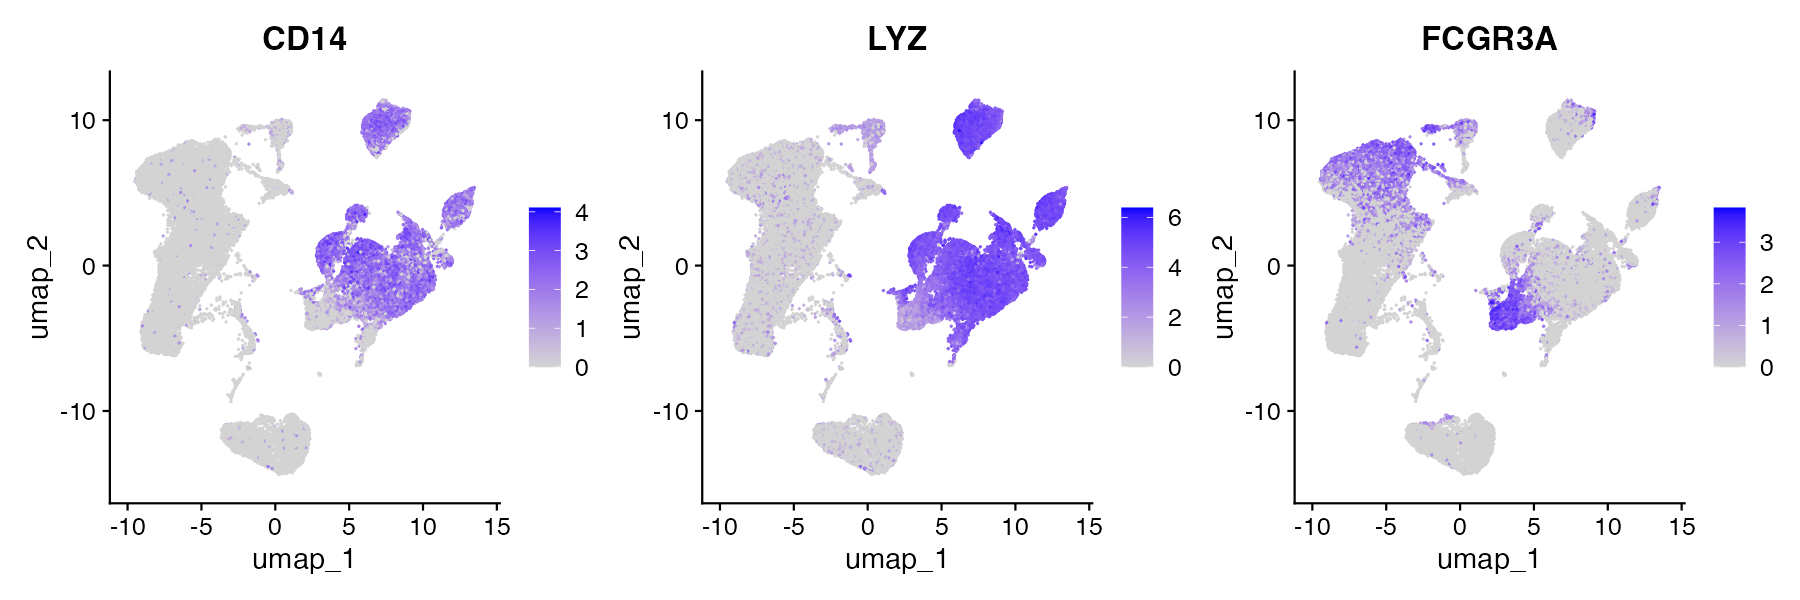
\includegraphics[width=\textwidth]{plots/phase3/phase3_step08a_markers_monocytes.png}
\end{center}

\begin{itemize}[nosep]
  \item \textbf{LYZ} (lysozyme): The most broadly expressed monocyte marker.
        High throughout the entire right continent, including the top-right
        isolated island (cluster 6). LYZ is produced by virtually all monocytes
        and macrophages. This is consistent with LYZ being the dominant gene on PC1.
  \item \textbf{CD14}: Expressed in the central-right mass but with lower levels
        than LYZ. CD14 is the lipopolysaccharide (LPS) co-receptor and marks
        \textbf{classical CD14$^+$ monocytes}. The slightly more restricted
        pattern compared to LYZ reflects the fact that non-classical monocytes
        downregulate CD14.
  \item \textbf{FCGR3A} (CD16): A different pattern from CD14 — high in a
        distinct sub-region of the right continent (mid-right to upper-right) but
        low in the central mass where CD14 is high. CD16 marks
        \textbf{non-classical/intermediate monocytes}. The spatial separation of
        CD14-high and FCGR3A-high cells in the UMAP suggests that the Louvain
        clustering at res = 0.5 is genuinely separating CD14$^+$ classical
        from CD14$^{\text{lo}}$/CD16$^+$ non-classical monocytes.
\end{itemize}

\paragraph*{T cell markers — CD3D, CD3E, CD4, CD8A}

\begin{center}
  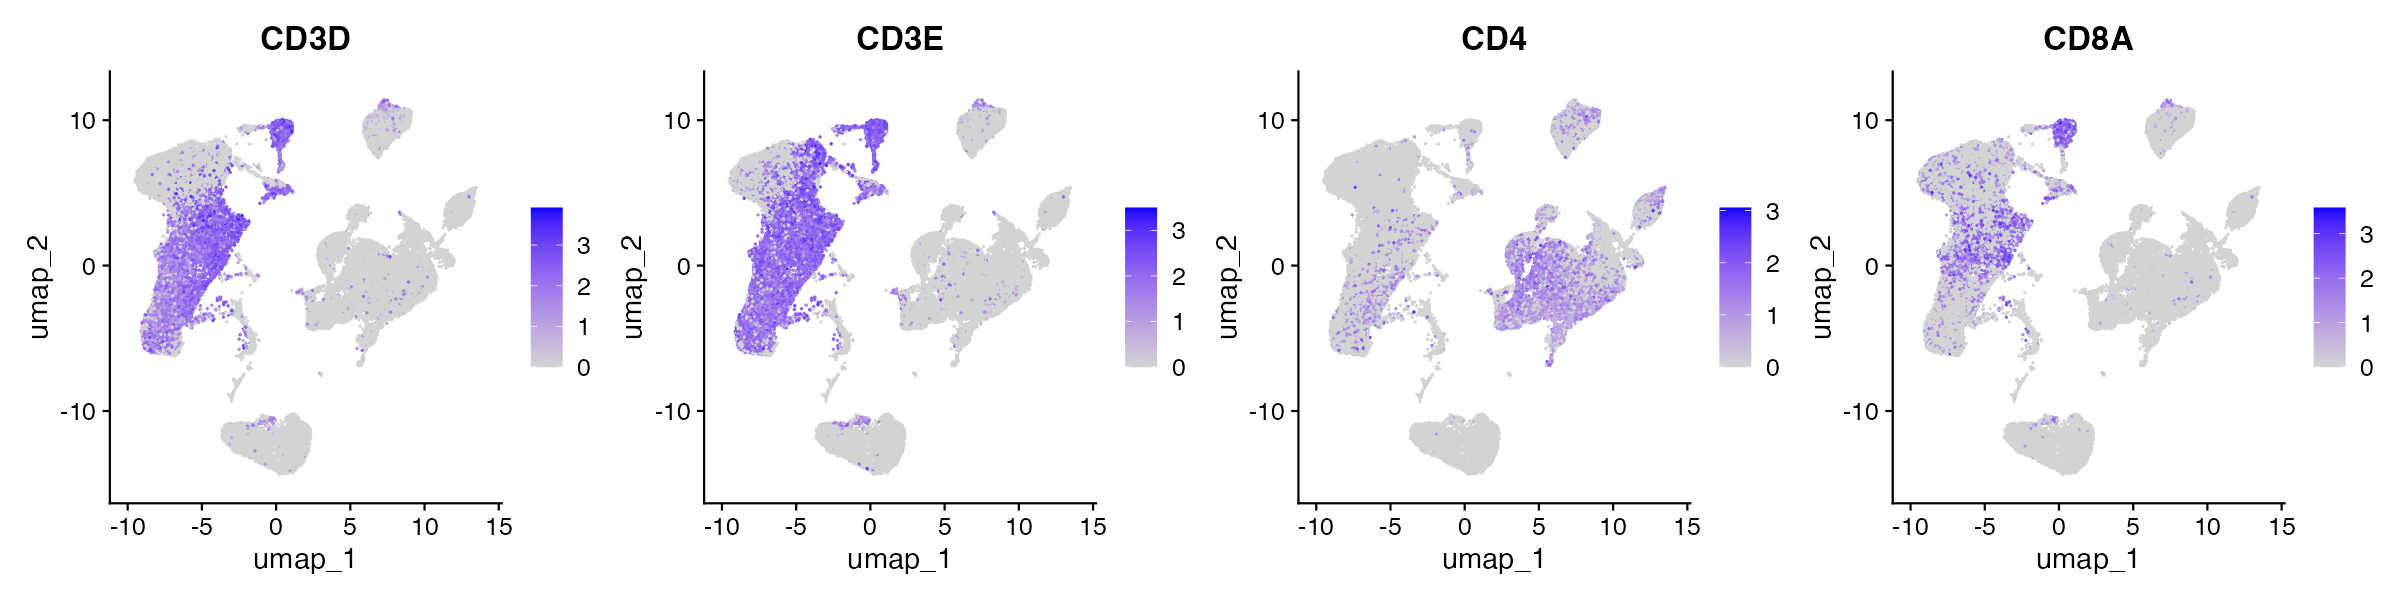
\includegraphics[width=\textwidth]{plots/phase3/phase3_step08b_markers_tcells.png}
\end{center}

\begin{itemize}[nosep]
  \item \textbf{CD3D and CD3E}: Both pan-T cell markers (components of the T cell
        receptor complex) light up the entire left continent, confirming that the
        left side is the T cell compartment. They are essentially interchangeable
        at this resolution.
  \item \textbf{CD4}: Restricted to the \textbf{lower-left} portion of the left
        continent. CD4 marks T helper cells and is absent from the upper-left
        region. The lower-left clusters (cluster 1 from the numbered UMAP) are
        \textbf{CD4$^+$ T helper cells}.
  \item \textbf{CD8A}: High in the \textbf{upper-left} portion of the left
        continent, in a region that overlaps but does not fully coincide with
        the NK cell zone. CD8$^+$ cytotoxic T cells and NK cells are
        transcriptionally similar (both cytotoxic) and sit adjacent on the UMAP.
        Cluster 0 (the large upper-left blob) likely mixes CD8$^+$ T and NK cells,
        consistent with the ambiguous marker patterns.
\end{itemize}

\paragraph*{B cell markers — MS4A1 (CD20), CD79A}

\begin{center}
  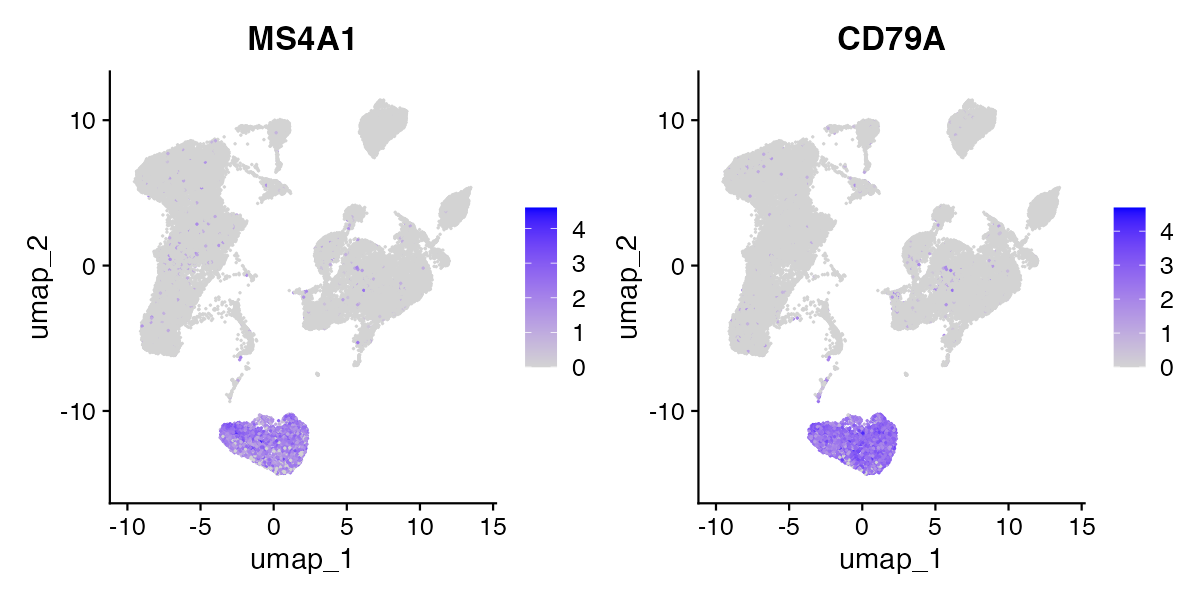
\includegraphics[width=\textwidth]{plots/phase3/phase3_step08c_markers_bcells.png}
\end{center}

Both B cell markers are expressed \textbf{exclusively} in the bottom isolated island
(clusters 5 and 9), with essentially zero expression everywhere else in the UMAP.
This is one of the clearest patterns in the dataset — the bottom island is entirely
B cells, and the gene markers have near-perfect specificity.
The fact that B cells form a completely isolated UMAP island reflects their
fundamentally different transcriptional programme compared to both myeloid and
T/NK cells — they express immunoglobulin genes (IGHM, IGKC), CD79A/B, and MS4A1,
none of which are expressed in other PBMC populations.

\paragraph*{NK cell markers — NKG7, GNLY}

\begin{center}
  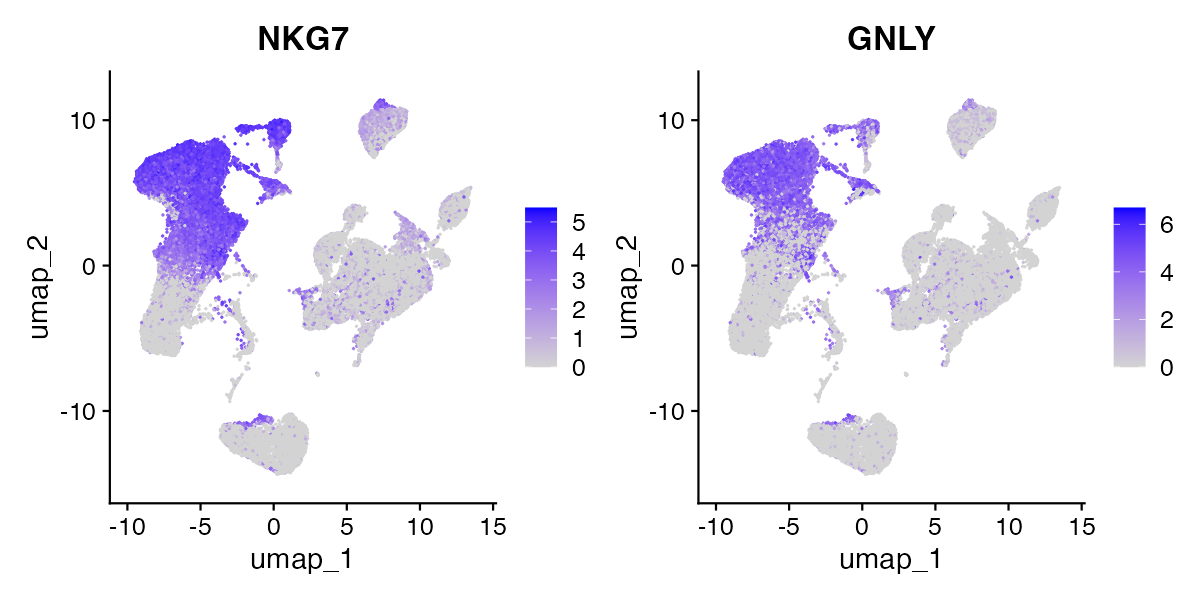
\includegraphics[width=\textwidth]{plots/phase3/phase3_step08d_markers_nk.png}
\end{center}

NKG7 and GNLY (granulysin) are expressed broadly across the \textbf{upper-left}
portion of the left continent, the same region where CD8A is also high.
This overlap is expected: NKG7 and GNLY are cytotoxic granule proteins expressed
by both cytotoxic T cells and NK cells. The SingleR cross-tabulation (Step 9)
will distinguish them by comparing the full expression profile against a reference
rather than relying on these few genes alone.

\paragraph*{Dot plot — canonical markers by cluster}

\begin{center}
  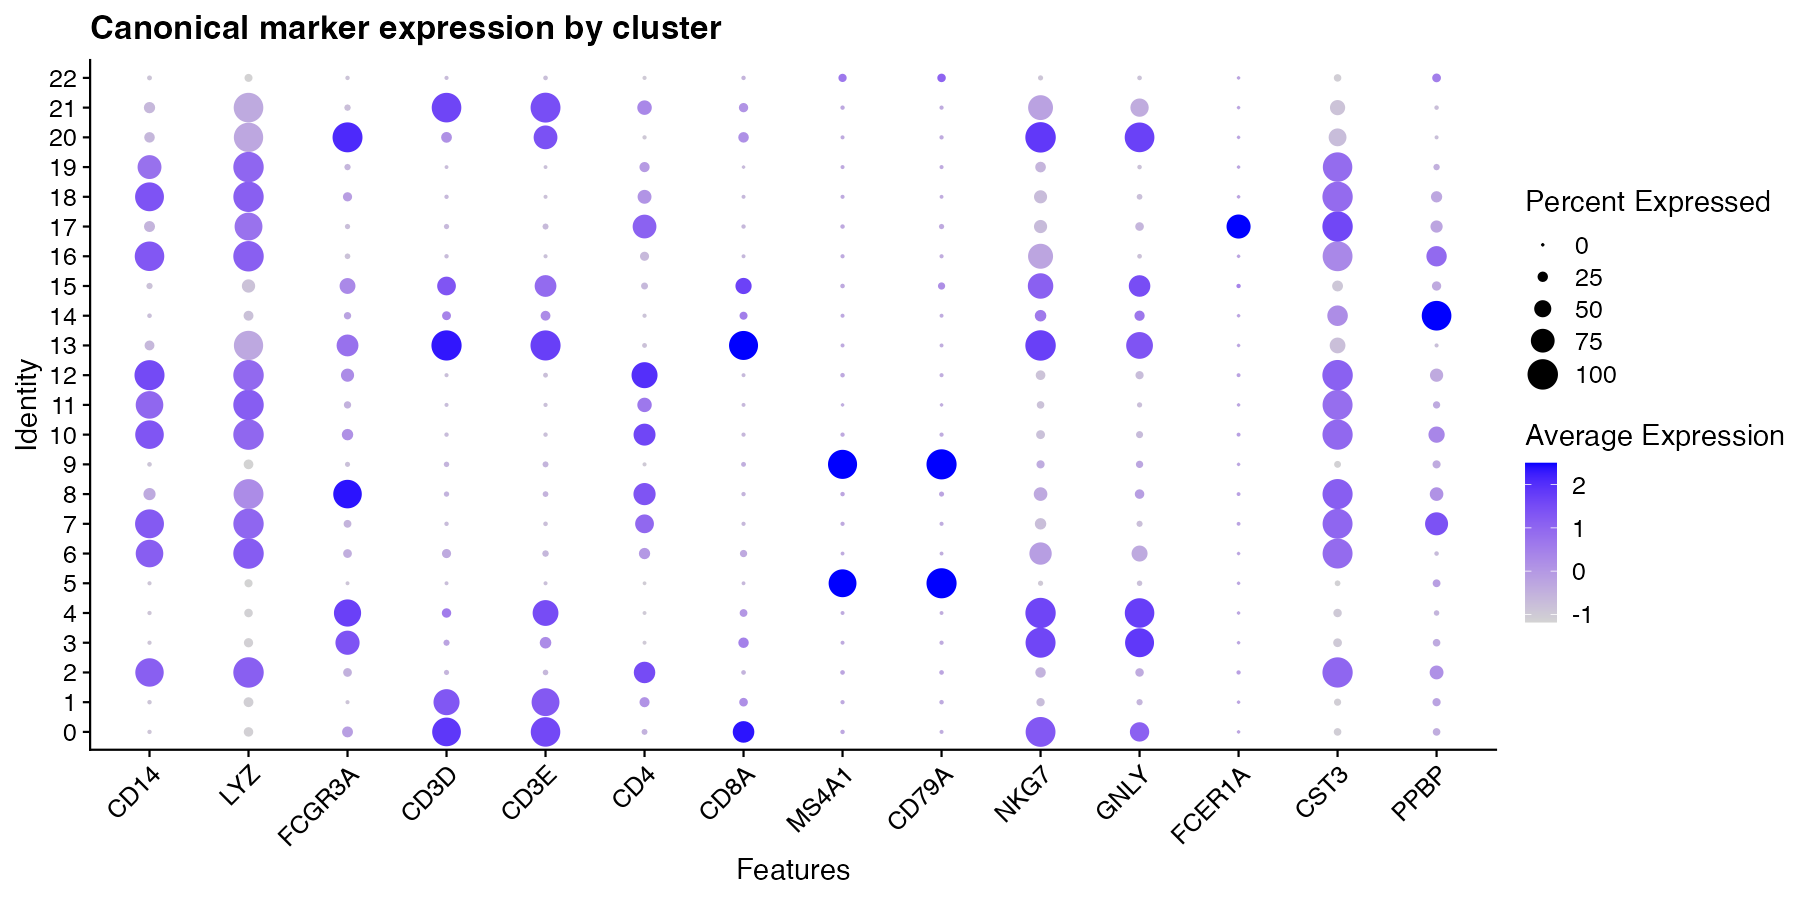
\includegraphics[width=\textwidth]{plots/phase3/phase3_step08e_dotplot_markers.png}
\end{center}

The dot plot shows all 14 canonical markers across all 23 clusters simultaneously.
Dot size = fraction of cells in the cluster expressing the gene;
dot colour = average scaled expression.
Reading across each row reveals the dominant identity of each cluster:

\begin{itemize}[nosep]
  \item \textbf{Clusters 2, 6, 7, 8, 10, 11, 12, 16, 18, 19}: Large blue dots
        for CD14 and LYZ, negligible T/B/NK markers
        $\to$ \textbf{classical CD14$^+$ monocytes} (multiple sub-clusters).
  \item \textbf{Cluster 8}: High FCGR3A in addition to LYZ
        $\to$ likely \textbf{CD16$^+$ non-classical monocytes}.
  \item \textbf{Clusters 0, 13}: High CD8A, NKG7, GNLY; minimal CD14
        $\to$ \textbf{CD8$^+$ T cells / NK cells}.
  \item \textbf{Cluster 1}: High CD3D, CD3E, CD4
        $\to$ \textbf{CD4$^+$ T cells}.
  \item \textbf{Clusters 3, 4, 20}: High NKG7, GNLY; low/absent CD3D
        $\to$ \textbf{NK cells}.
  \item \textbf{Clusters 5, 9}: High MS4A1, CD79A; all other markers near zero
        $\to$ \textbf{B cells}.
  \item \textbf{Cluster 14}: High PPBP; mixed low expression of other markers
        $\to$ \textbf{platelets / megakaryocytes}. This is where the PC2
        platelet signal from Phase 2 actually maps to.
  \item \textbf{Cluster 17}: Low-level CST3 and FCER1A signal
        $\to$ candidate \textbf{dendritic cells}.
  \item \textbf{Clusters 15, 21}: Mixed T/NK signal
        $\to$ likely T cell sub-states (memory, regulatory, or transitional).
\end{itemize}

\subsubsection*{Step 9 — SingleR automated annotation}

SingleR compares each cell's full expression profile against the
BlueprintEncode bulk RNA-seq reference (which contains sorted immune cell
populations) and assigns the closest matching label to every cell independently.

\paragraph*{Label distribution.}
After annotating all 55,548 cells:

\begin{center}
\begin{tabular}{lrr}
\hline
\textbf{Cell type} & \textbf{Cells} & \textbf{\%} \\
\hline
Monocytes        & 21,385 & 38.5\% \\
NK cells         & 11,396 & 20.5\% \\
CD8$^+$ T-cells  & 10,471 & 18.8\% \\
B-cells          &  6,665 & 12.0\% \\
CD4$^+$ T-cells  &  4,990 &  9.0\% \\
Erythrocytes     &    410 &  0.7\% \\
HSC              &    108 &  0.2\% \\
Neutrophils      &     71 &  0.1\% \\
Eosinophils      &     46 &  0.1\% \\
DC               &      5 & $<$0.1\% \\
Endothelial cells &     1 & $<$0.1\% \\
\hline
\end{tabular}
\end{center}

The monocyte dominance (38.5\%) is a known hallmark of severe COVID-19 infection —
Li et al.\ and multiple cohort studies have documented emergency myelopoiesis driving
monocyte expansion in severe disease. NK cell enrichment (20.5\%) is also higher than
healthy PBMC baselines, consistent with innate immune activation.

The CD4$^+$ T cell count (9.0\%) is notably low compared to healthy PBMCs where
CD4$^+$ T cells typically constitute 30--40\% of lymphocytes. This T cell depletion
is another well-replicated feature of severe COVID-19: lymphopenia affecting preferentially
the helper T cell compartment.

The rare populations (Erythrocytes, HSC, Neutrophils, Eosinophils) are either
contamination, uncommitted progenitors, or cells that the BlueprintEncode reference
is forced to assign to the nearest-available label when the true cell type is absent
from its training data.

\paragraph*{UMAP coloured by SingleR labels.}

\begin{center}
  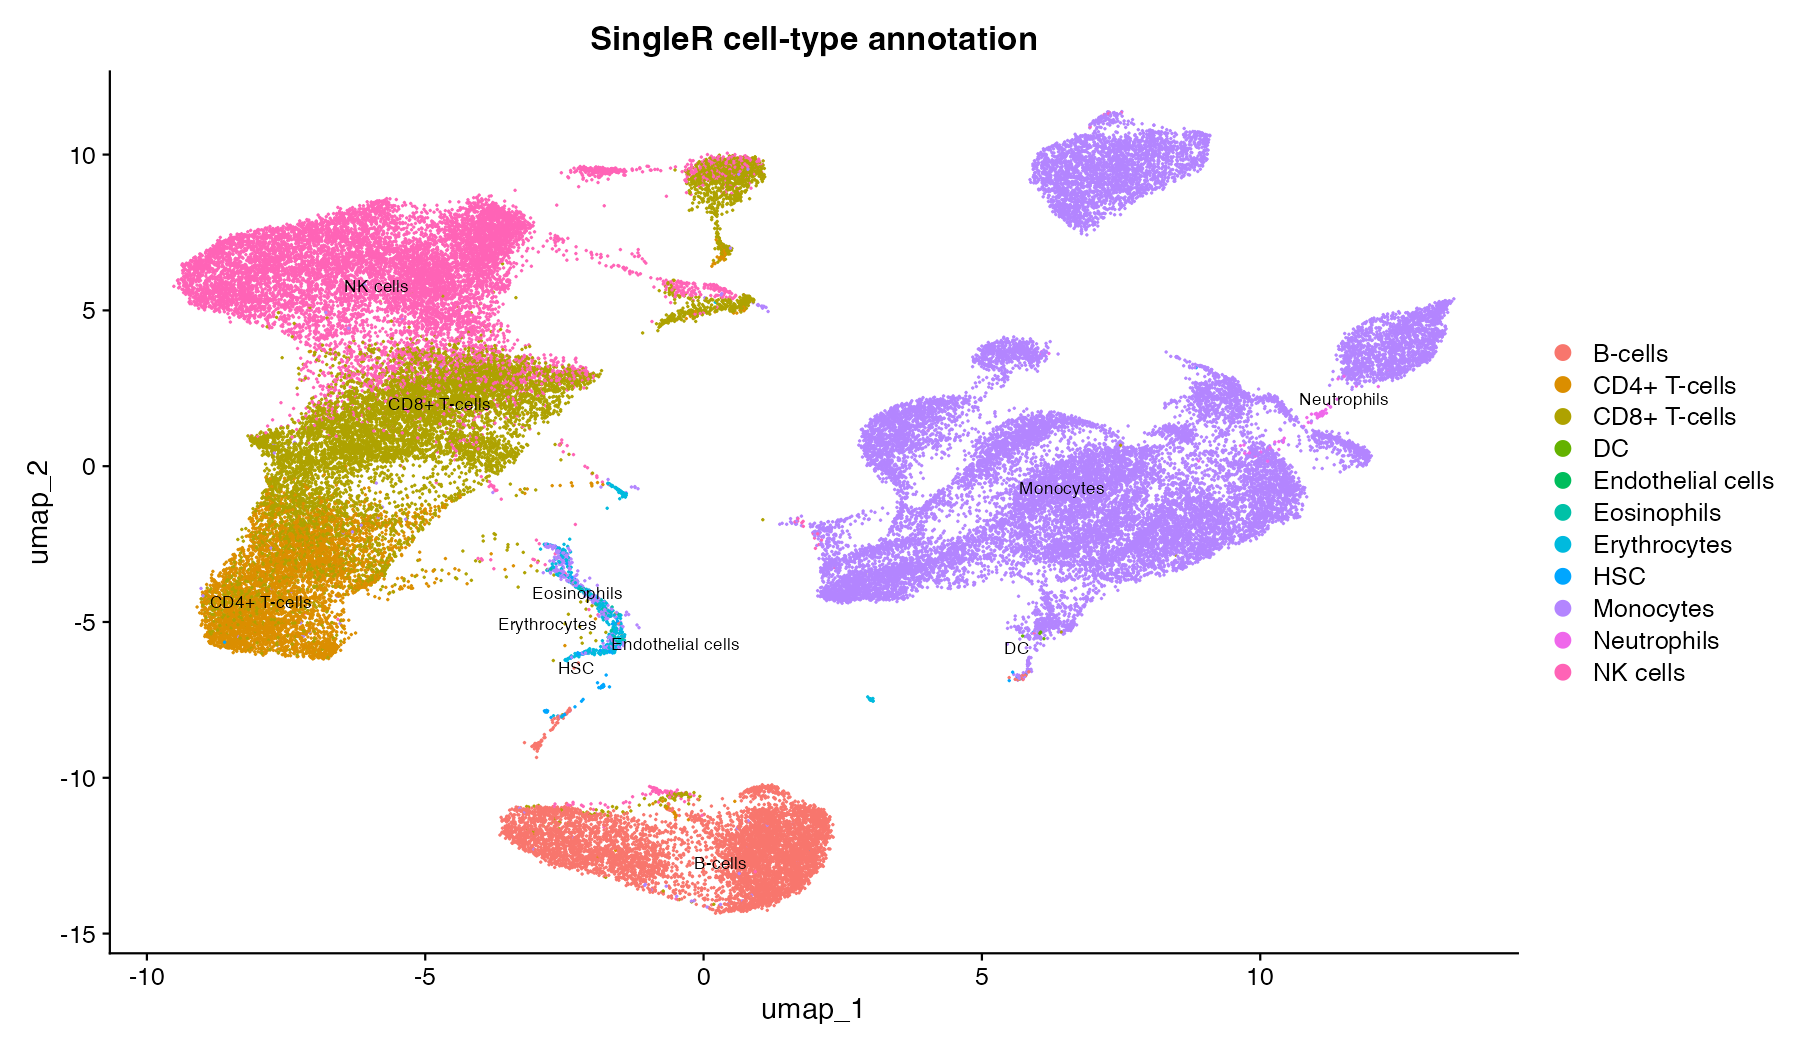
\includegraphics[width=0.95\textwidth]{plots/phase3/phase3_step09c_umap_singler.png}
\end{center}

The SingleR UMAP confirms all marker-based identifications and resolves the
CD8$^+$ T vs NK cell ambiguity:

\begin{itemize}[nosep]
  \item \textbf{Right continent} = Monocytes (purple), filling the entire right mass
        and the top-right isolated island (cluster 6). The spatial coherence of the
        monocyte annotation across all right-side clusters is excellent.
  \item \textbf{Upper-left continent} = NK cells (pink) dominating the upper portion;
        CD8$^+$ T-cells (olive) occupying the middle of the left continent.
  \item \textbf{Lower-left continent} = CD4$^+$ T-cells (orange/gold) in the
        lower-left pocket — cleanly separated from both NK and CD8$^+$ populations.
  \item \textbf{Bottom island} = B-cells (salmon/pink), completely isolated, confirming
        the MS4A1/CD79A feature plot result. Both cluster 5 and cluster 9 are
        overwhelmingly B cells.
  \item \textbf{Center transition zone (cluster 14)} = a mixed cluster of Erythrocytes,
        HSC, Eosinophils, Neutrophils, and Monocytes — this is the ``garbage bin''
        cluster for cells that don't fit cleanly into any major population.
        The PPBP (platelet) signal from the dot plot also maps here.
  \item \textbf{Top-centre isolated group} = mixed CD8$^+$ T and NK cells
        (the green DC dots are from the 5 DC-labelled cells in the dataset).
\end{itemize}

\paragraph*{dittoSeq UMAP.}

\begin{center}
  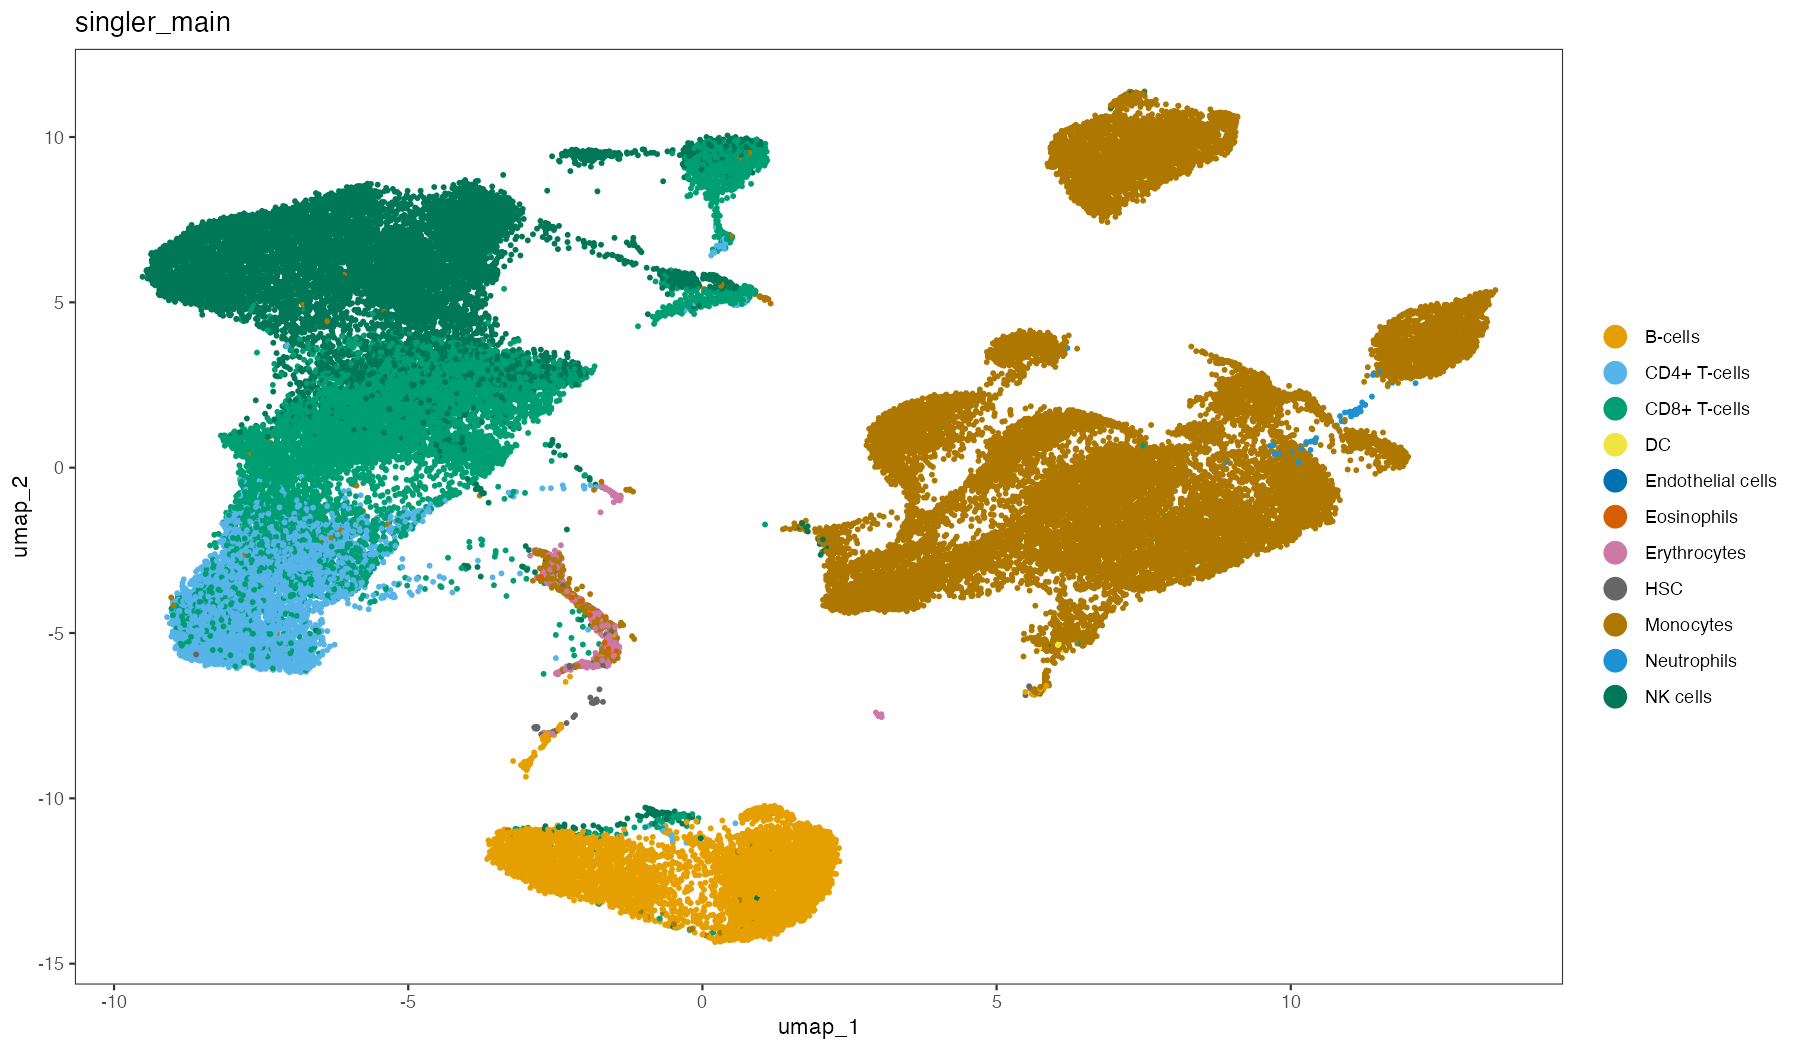
\includegraphics[width=0.95\textwidth]{plots/phase3/phase3_step09d_ditto_umap.png}
\end{center}

The dittoSeq plot (which uses a color-blind-friendly palette and a slightly different
layout algorithm) confirms the same overall structure. The clean agreement between
the standard \texttt{DimPlot} and the dittoSeq plot rules out any color mapping
artefact: the population assignments are robust.

\paragraph*{Cross-tabulation — clusters vs SingleR labels.}

The cross-tabulation shows how many cells of each SingleR type fall in each
graph-based cluster. The ideal result is that each cluster is dominated by a
single cell type (high purity). The results:

\begin{itemize}[nosep]
  \item \textbf{Pure clusters ($>$95\% one type):}
        Clusters 2, 5, 6, 7, 9, 10, 11, 12, 16, 18, 19 (monocytes);
        clusters 3, 4, 20 (NK cells); clusters 5, 9 (B cells, 100\%).
        This is the expected result for well-chosen resolution — the
        algorithm found real biological boundaries.
  \item \textbf{Mixed clusters:}
        Cluster 0 (CD8$^+$ + NK: 6669 vs 1151) and cluster 13 (CD8$^+$ + NK:
        1012 vs 324) reflect the transcriptional similarity between CD8$^+$ T cells
        and NK cells — both are cytotoxic and express similar granule genes.
        Cluster 1 (CD4$^+$ + CD8$^+$: 4853 vs 1892) suggests a transition zone
        between the two T cell sub-populations.
  \item \textbf{Cluster 14 — the heterogeneous cluster:}
        Monocytes (338), CD8$^+$ T (167), NK (144), Erythrocytes (318), HSC (58),
        Eosinophils (46). This cluster sits in the UMAP transition zone between
        the two continents. It captures cells that are transcriptionally
        intermediate — likely a mix of contaminating non-lymphoid cells
        (red blood cells, platelet-associated cells) and cells in transitional states.
        In downstream Phase 4 analysis, monocytes will be isolated by the
        \texttt{singler\_main == "Monocytes"} label, so cluster 14 contamination
        will be correctly excluded.
\end{itemize}

\paragraph*{Overall assessment.}
The manual marker approach and SingleR agree on all major populations.
The five main PBMC compartments are all present and correctly localized:
monocytes (right), NK cells (upper-left), CD8$^+$ T cells (middle-left),
CD4$^+$ T cells (lower-left), B cells (bottom island).
The enrichment pattern — monocyte-dominant, CD4$^+$ T cell-depleted — is
consistent with published COVID-19 PBMC immunophenotypes.

\subsection{Find cluster-defining markers \small\normalfont\textit{(Step 10)}}

\texttt{FindAllMarkers()} compares each cluster against all remaining cells
using the Wilcoxon rank-sum test, asking: which genes are expressed at a
significantly higher level in this cluster than everywhere else?
A gene passes the filter if it is detected in $\geq$25\% of cells in the
cluster (\texttt{min.pct = 0.25}) and shows at least a 2-fold difference
(\texttt{logfc.threshold = 0.5} on the log$_2$ scale).
\textbf{6,739 markers} were found across all 23 clusters, all with adjusted
p-value = 0 (exact zeros arise because the values underflow floating-point
precision — in practice these are extremely small numbers, far below 0.001).

Due to the 16 GB memory constraint on this machine, \texttt{FindAllMarkers}
was run on a downsampled object (300 cells per cluster; 6,513 cells total
drawn with \texttt{set.seed(42)}). The same variable features (3,000 genes)
from the full object were used. At 300 cells per cluster the statistical
power is sufficient to recover all highly expressed, cluster-specific markers.

\subsubsection*{Heatmap — top 5 markers per cluster}

\begin{center}
  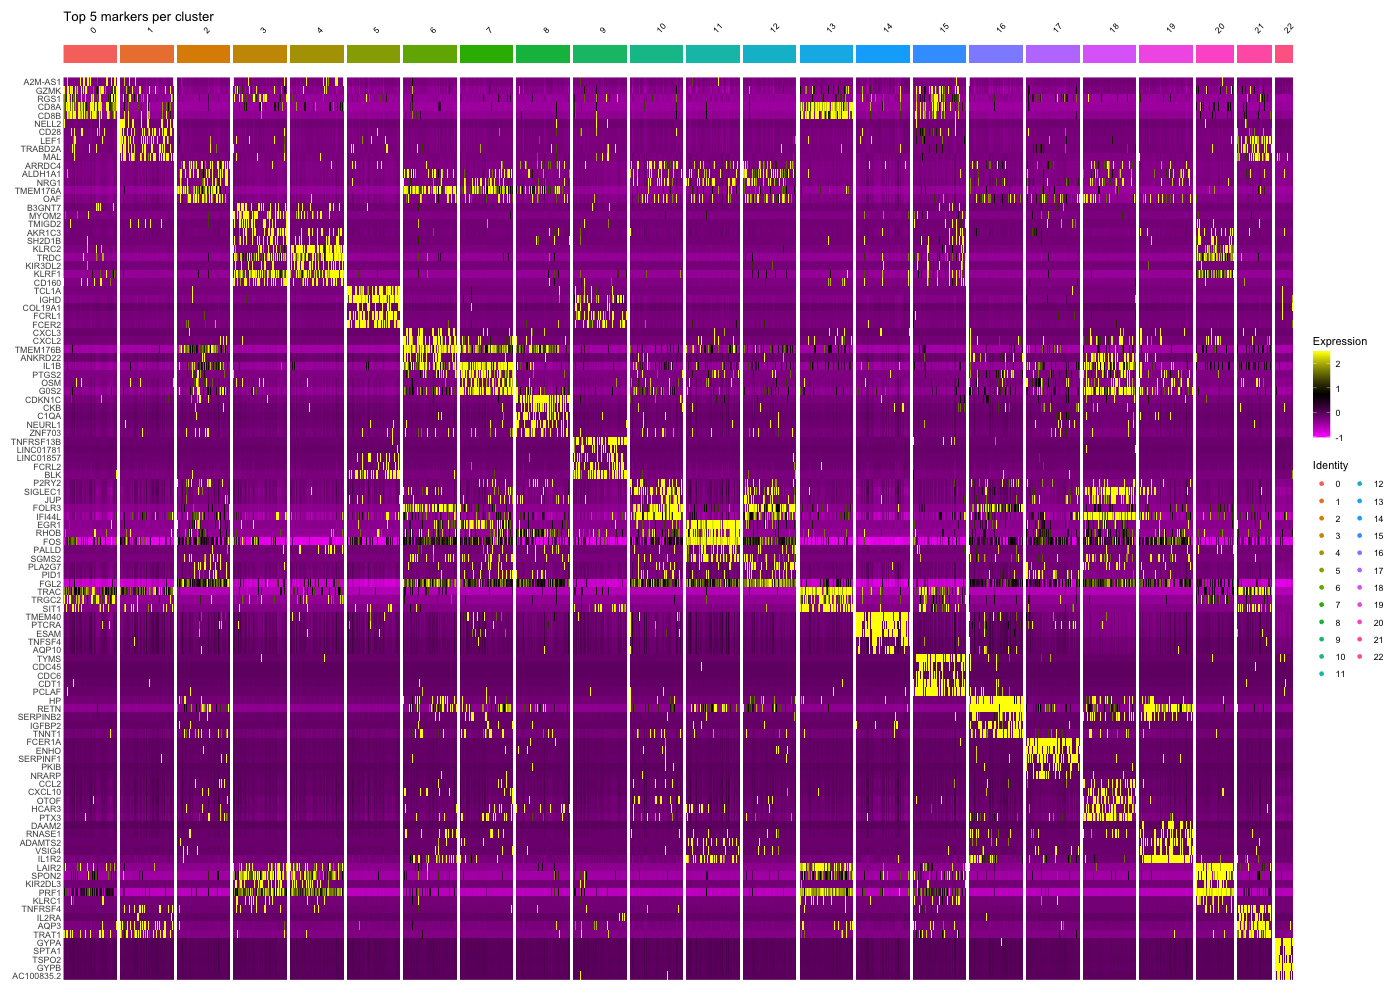
\includegraphics[width=\textwidth]{plots/phase3/phase3_step10a_marker_heatmap.png}
\end{center}

Yellow = high expression; purple = low or absent.
Each column block is one cluster; each row is one gene.
A good marker produces a bright yellow stripe in exactly one cluster and is
dark everywhere else.
The heatmap shows clean diagonal structure: most genes are specific to one
cluster, confirming high cluster purity and biologically meaningful separation.

\subsubsection*{Cluster identity table (from top-5 markers)}

Reading the marker genes for each cluster and cross-referencing with the
literature gives the following cell-type assignments:

\begin{center}
\small
\begin{tabular}{cll}
\hline
\textbf{Cluster} & \textbf{Cell type} & \textbf{Key markers} \\
\hline
0  & CD8$^+$ T cells (effector memory) & GZMK, CD8A, CD8B, RGS1 \\
1  & Naive / central-memory CD4$^+$ T & LEF1, CD28, MAL, NELL2 \\
2  & Monocyte sub-cluster & TMEM176A, ALDH1A1 \\
3  & NK cells                           & TMIGD2, SH2D1B, AKR1C3 \\
4  & NK / $\gamma\delta$ T cells        & KLRC2, TRDC, KIR3DL2, KLRF1 \\
5  & Naive B cells                      & TCL1A, IGHD, FCER2, FCRL1 \\
6  & Inflammatory monocytes             & CXCL2, CXCL3, TMEM176A/B \\
7  & IL-1$\beta$$^+$ monocytes (inflammasome-active) & IL1B, PTGS2, OSM \\
8  & Non-classical (CD16$^+$) monocytes & CDKN1C, C1QA, CKB \\
9  & Memory B cells                     & TNFRSF13B, FCRL2, BLK \\
10 & ISG-high monocytes                 & SIGLEC1, IFI44L, FOLR3 \\
11 & Stress-response / early-activation monocytes & EGR1, FOS, RHOB \\
12 & Mature/tissue-like monocytes       & PLA2G7, FGL2, FOLR3 \\
13 & CD8$^+$ T / $\gamma\delta$ T cells & CD8A, CD8B, TRAC, TRGC2 \\
14 & Platelets / megakaryocytes         & PTCRA, ESAM, TMEM40, AQP10 \\
15 & Proliferating cells (S phase)      & TYMS, CDC45, CDC6, CDT1, PCLAF \\
16 & Immature / emergency monocytes     & HP, RETN, SERPINB2 \\
17 & Dendritic cells (cDC2 / pDC)       & FCER1A, ENHO, SERPINF1 \\
18 & CXCL10$^+$/CCL2$^+$ monocytes (IFN-chemokine) & CCL2, CXCL10, PTX3 \\
19 & Immunosuppressive / resident-like monocytes & VSIG4, IL1R2, RNASE1 \\
20 & Cytotoxic NK cells                 & PRF1, KIR2DL3, KLRC1, LAIR2 \\
21 & CD4$^+$ Tregs / activated CD4$^+$ T & IL2RA (CD25), TNFRSF4 (OX40) \\
22 & Erythrocytes (contamination)       & GYPA, GYPB, SPTA1 \\
\hline
\end{tabular}
\end{center}

\subsubsection*{Biologically noteworthy clusters}

Several clusters stand out as directly relevant to the COVID-19 biology:

\begin{itemize}[nosep]
  \item \textbf{Cluster 7 — IL-1$\beta^+$ monocytes:}
        The top marker is \textit{IL1B} (avg log$_2$FC = 3.37, expressed in
        90\% of cells in this cluster vs 23\% everywhere else).
        \textit{PTGS2} (COX-2) and \textit{OSM} (oncostatin M) follow.
        IL-1$\beta$, COX-2, and OSM together define a fully activated
        inflammasome program — this is the stereotypic severe-COVID
        hyper-inflammatory monocyte state. This cluster is critically
        important for Phase 4.

  \item \textbf{Cluster 10 — ISG-high monocytes:}
        \textit{SIGLEC1} (CD169) at log$_2$FC = 3.32 is the canonical marker
        of type-I interferon-stimulated monocytes. \textit{IFI44L} (IFN-induced
        protein 44-like) confirms the interferon signature.
        SIGLEC1$^+$ monocytes are specifically expanded in severe COVID-19
        and are a known indicator of systemic interferon activation.

  \item \textbf{Cluster 18 — CCL2$^+$/CXCL10$^+$ monocytes:}
        \textit{CCL2} (MCP-1) and \textit{CXCL10} (IP-10/CXCL10) are the
        two most upregulated chemokines in severe COVID-19 plasma.
        Their expression at the single-cell level in this cluster identifies
        the specific monocyte sub-population responsible for secreting
        the inflammatory chemokine storm. \textit{PTX3} (pentraxin-3),
        also a top marker here, is an acute-phase protein produced by
        activated monocytes and known to be elevated in ICU-COVID patients.

  \item \textbf{Cluster 15 — Proliferating cells:}
        TYMS, CDC45, CDC6, CDT1, PCLAF are all S-phase DNA replication
        genes. This cluster captures immune cells actively dividing —
        consistent with emergency myelopoiesis (monocyte precursors
        proliferating in the bone marrow and spilling into blood)
        reported in severe COVID.

  \item \textbf{Cluster 22 — Erythrocytes:}
        log$_2$FC of 13.7 for \textit{GYPA} with only 0.0\% expression in
        all other cells is clean contamination. These are red blood cells
        that were not fully removed by the PBMC density gradient.
        They will not be included in the monocyte subset for Phase 4.

  \item \textbf{Cluster 21 — Tregs:}
        \textit{IL2RA} (CD25) and \textit{TNFRSF4} (OX40) together are a
        strong Treg signature. CD25$^+$OX40$^+$ T cells are regulatory T cells.
        Their presence at relatively low numbers is consistent with the known
        COVID-19 pattern of Treg dysfunction.
\end{itemize}

\subsection{Phase 3 conclusion}

Phase 3 successfully identified and annotated all major PBMC populations.
The 23 clusters at resolution 0.5 span a rich diversity of cell states:

\begin{itemize}[nosep]
  \item \textbf{Myeloid:} 10 monocyte sub-clusters covering classical,
        non-classical, inflammatory (IL-1$\beta^+$), ISG-high, chemokine-secreting,
        immunosuppressive, and immature monocyte states — reflecting the
        complexity of monocyte dysregulation in COVID-19.
  \item \textbf{Lymphoid:} CD8$^+$ effector memory T cells, naive and central
        memory CD4$^+$ T cells, cytotoxic NK cells, $\gamma\delta$ T cells,
        and Tregs.
  \item \textbf{B cells:} Naive B cells (cluster 5) and memory B cells (cluster 9).
  \item \textbf{Other:} Dendritic cells, proliferating cells, and two
        contamination clusters (platelets/cluster 14, erythrocytes/cluster 22).
\end{itemize}

The annotated object is saved to \texttt{Data/phase3\_seurat\_annotated.rds}
and the full marker table to \texttt{Data/phase3\_all\_markers.csv}
for use in Phase 4.

% ─────────────────────────────────────────────────────────
\subsection{Module scoring — what it is and why we use it}

After annotating cell types in Phase 3, the next question is:
\textit{``How active is a specific program in each individual cell?''}
We do not want a yes/no answer — we want a continuous number that says
\textit{how strongly} a cell is running the antiviral program or the
inflammatory program.

\textbf{Module scoring} (\texttt{AddModuleScore} in Seurat) does exactly this.

\subsubsection*{The simple idea}

You give the function a list of genes that together define a biological program
(the ``module''). For each cell, it computes the average expression of those
genes, then subtracts the average expression of a set of randomly chosen
background genes.

\begin{itemize}[nosep]
  \item A \textbf{positive score} means the cell expresses your module genes
        more than random background — the program is active.
  \item A \textbf{negative score} means the program is off or below background.
  \item The score is \textbf{continuous} — you can compare how strongly
        different cells have the program on.
\end{itemize}

There is no fixed threshold built into the method.
A common choice is to call a cell ``active'' for a module when its score
exceeds zero, because the score is designed to be centered at zero for
backgroundlevels of expression.

\subsubsection*{The two modules used in this project}

\begin{itemize}[nosep]
  \item \textbf{ISG score} (antiviral program): ISG15, IFIT1, MX1, OAS1, IFI44L —
        all strong markers of type-I interferon activation.
  \item \textbf{TNF/IL-1$\beta$ score} (inflammatory program): TNF, IL1B, CCL3,
        CCL4, CXCL8 — the core cytokines of the pro-inflammatory monocyte response.
\end{itemize}

A cell is called \textbf{co-activated} when \textit{both} scores are above zero
simultaneously. This is the central measurement of this project.

% ─────────────────────────────────────────────
\section{Phase 4 — CD14\textsuperscript{+} Monocyte Deep-Dive}
% ─────────────────────────────────────────────

\subsection{Phase 4 overview — the big picture}

\textbf{Phase 3 found the cells. Phase 4 asks what those cells are doing — and whether disease severity changes it.}

By the end of Phase 3 we had 23 annotated clusters with several monocyte sub-states
(IL-1$\beta^+$, ISG-high, chemokine-secreting, etc.). But we had not yet connected
those states to disease severity, nor had we tested the central hypothesis:
do severe COVID monocytes run both the antiviral and inflammatory programs
\textit{at the same time}?

Phase 4 answers that question in five steps:

\begin{enumerate}[nosep]
  \item \textbf{Add severity labels} — attach Healthy/Mild/Severe/Flu to every cell.
  \item \textbf{Visualize composition} — does the balance of cell types shift with severity?
  \item \textbf{Subset monocytes} — isolate only the monocytes for focused analysis.
  \item \textbf{Score both programs} — measure ISG and TNF/IL-1$\beta$ activity per cell.
  \item \textbf{Test co-activation} — is the top-right quadrant (both high) enriched in severe COVID?
\end{enumerate}

\subsection{Add severity metadata and subset monocytes \small\normalfont\textit{(Steps 3–4)}}

Each cell in the dataset carries a barcode suffix that maps to one of 20 donors
from Lee et al.\ 2020. Using the paper's clinical table (Table S1), each donor
is assigned a severity label: \textbf{Severe COVID} (nCoV 1--7),
\textbf{Mild COVID} (nCoV 8--11), \textbf{Healthy} (Normal 1--4), or
\textbf{Flu} (Flu 1--5). This gives every single cell in the dataset a severity
label, not just an average across samples.

\textbf{Metadata summary after assignment:}
\begin{itemize}[nosep]
  \item 4 Healthy donors, 4 Mild donors, 7 Severe donors, 5 Flu donors.
  \item Monocytes subset: 21,385 cells (all cells labelled \texttt{Monocytes}
        by SingleR), covering all four severity groups.
\end{itemize}

\subsubsection*{Step 3a — UMAP split by severity}

\begin{center}
  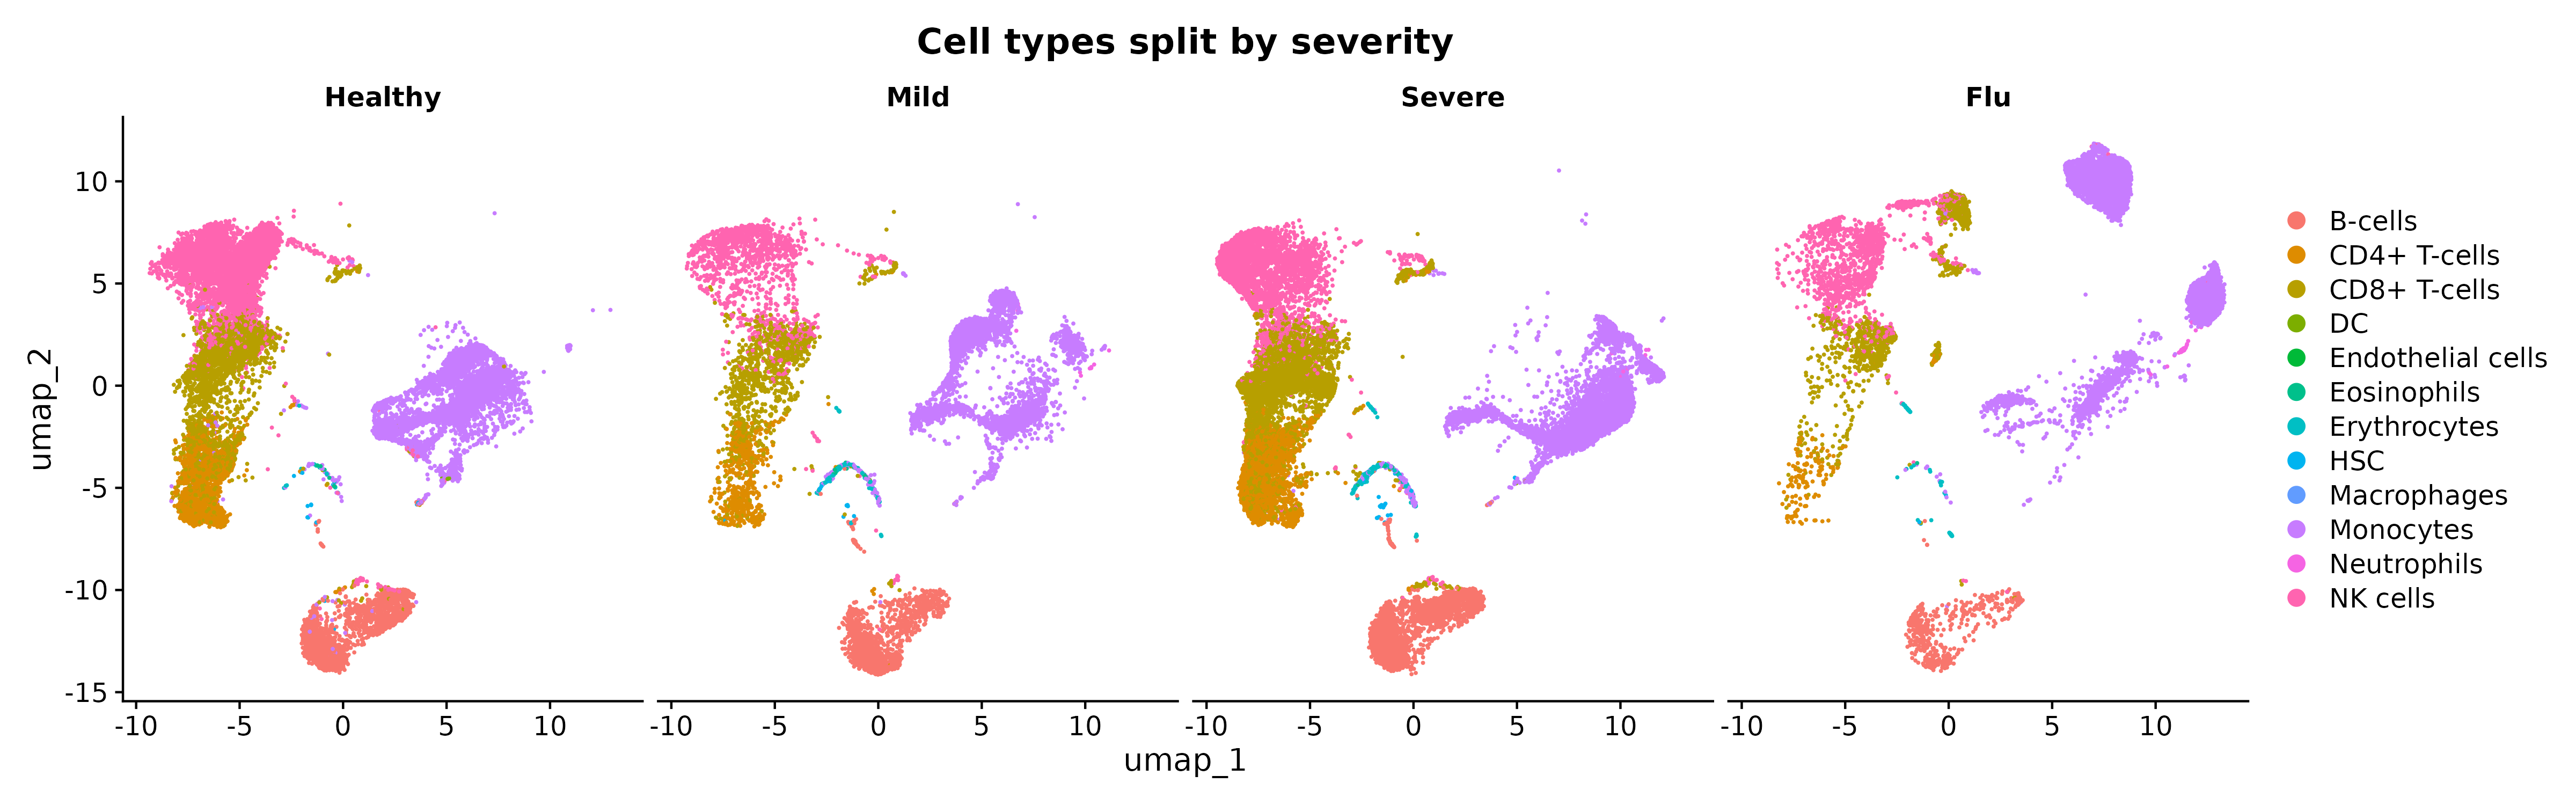
\includegraphics[width=\textwidth]{plots/phase4/phase4_umap_split_severity.png}
\end{center}

Each panel shows the same UMAP from Phase 3 but only with cells from one
severity group. Monocytes are purple; T and NK cells are gold/olive/pink;
B cells are salmon at the bottom island.

\begin{itemize}[nosep]
  \item \textbf{Healthy:} the UMAP is balanced. Monocytes occupy the right
        continent (purple), but T and NK cells fill the left continent with
        comparable density. No single cell type dominates.
  \item \textbf{Mild:} broadly similar to Healthy. Monocytes are present in the
        right continent; the T/NK left side is still well-populated.
  \item \textbf{Severe:} the right continent (monocytes) is clearly denser and
        more filled-in. The left continent (T cells, NK cells) appears thinner.
        This is the \textbf{monocyte expansion + lymphopenia} pattern typical of
        severe COVID-19.
  \item \textbf{Flu:} the monocyte continent dominates even more than Severe —
        and, strikingly, a separate isolated monocyte blob appears in the top-right
        corner of the Flu UMAP. This suggests a Flu-specific monocyte sub-state
        that is transcriptionally distinct enough to detach from the main monocyte
        mass in the embedding.
\end{itemize}

\subsubsection*{Step 3b — Cell-type composition by severity}

\begin{center}
  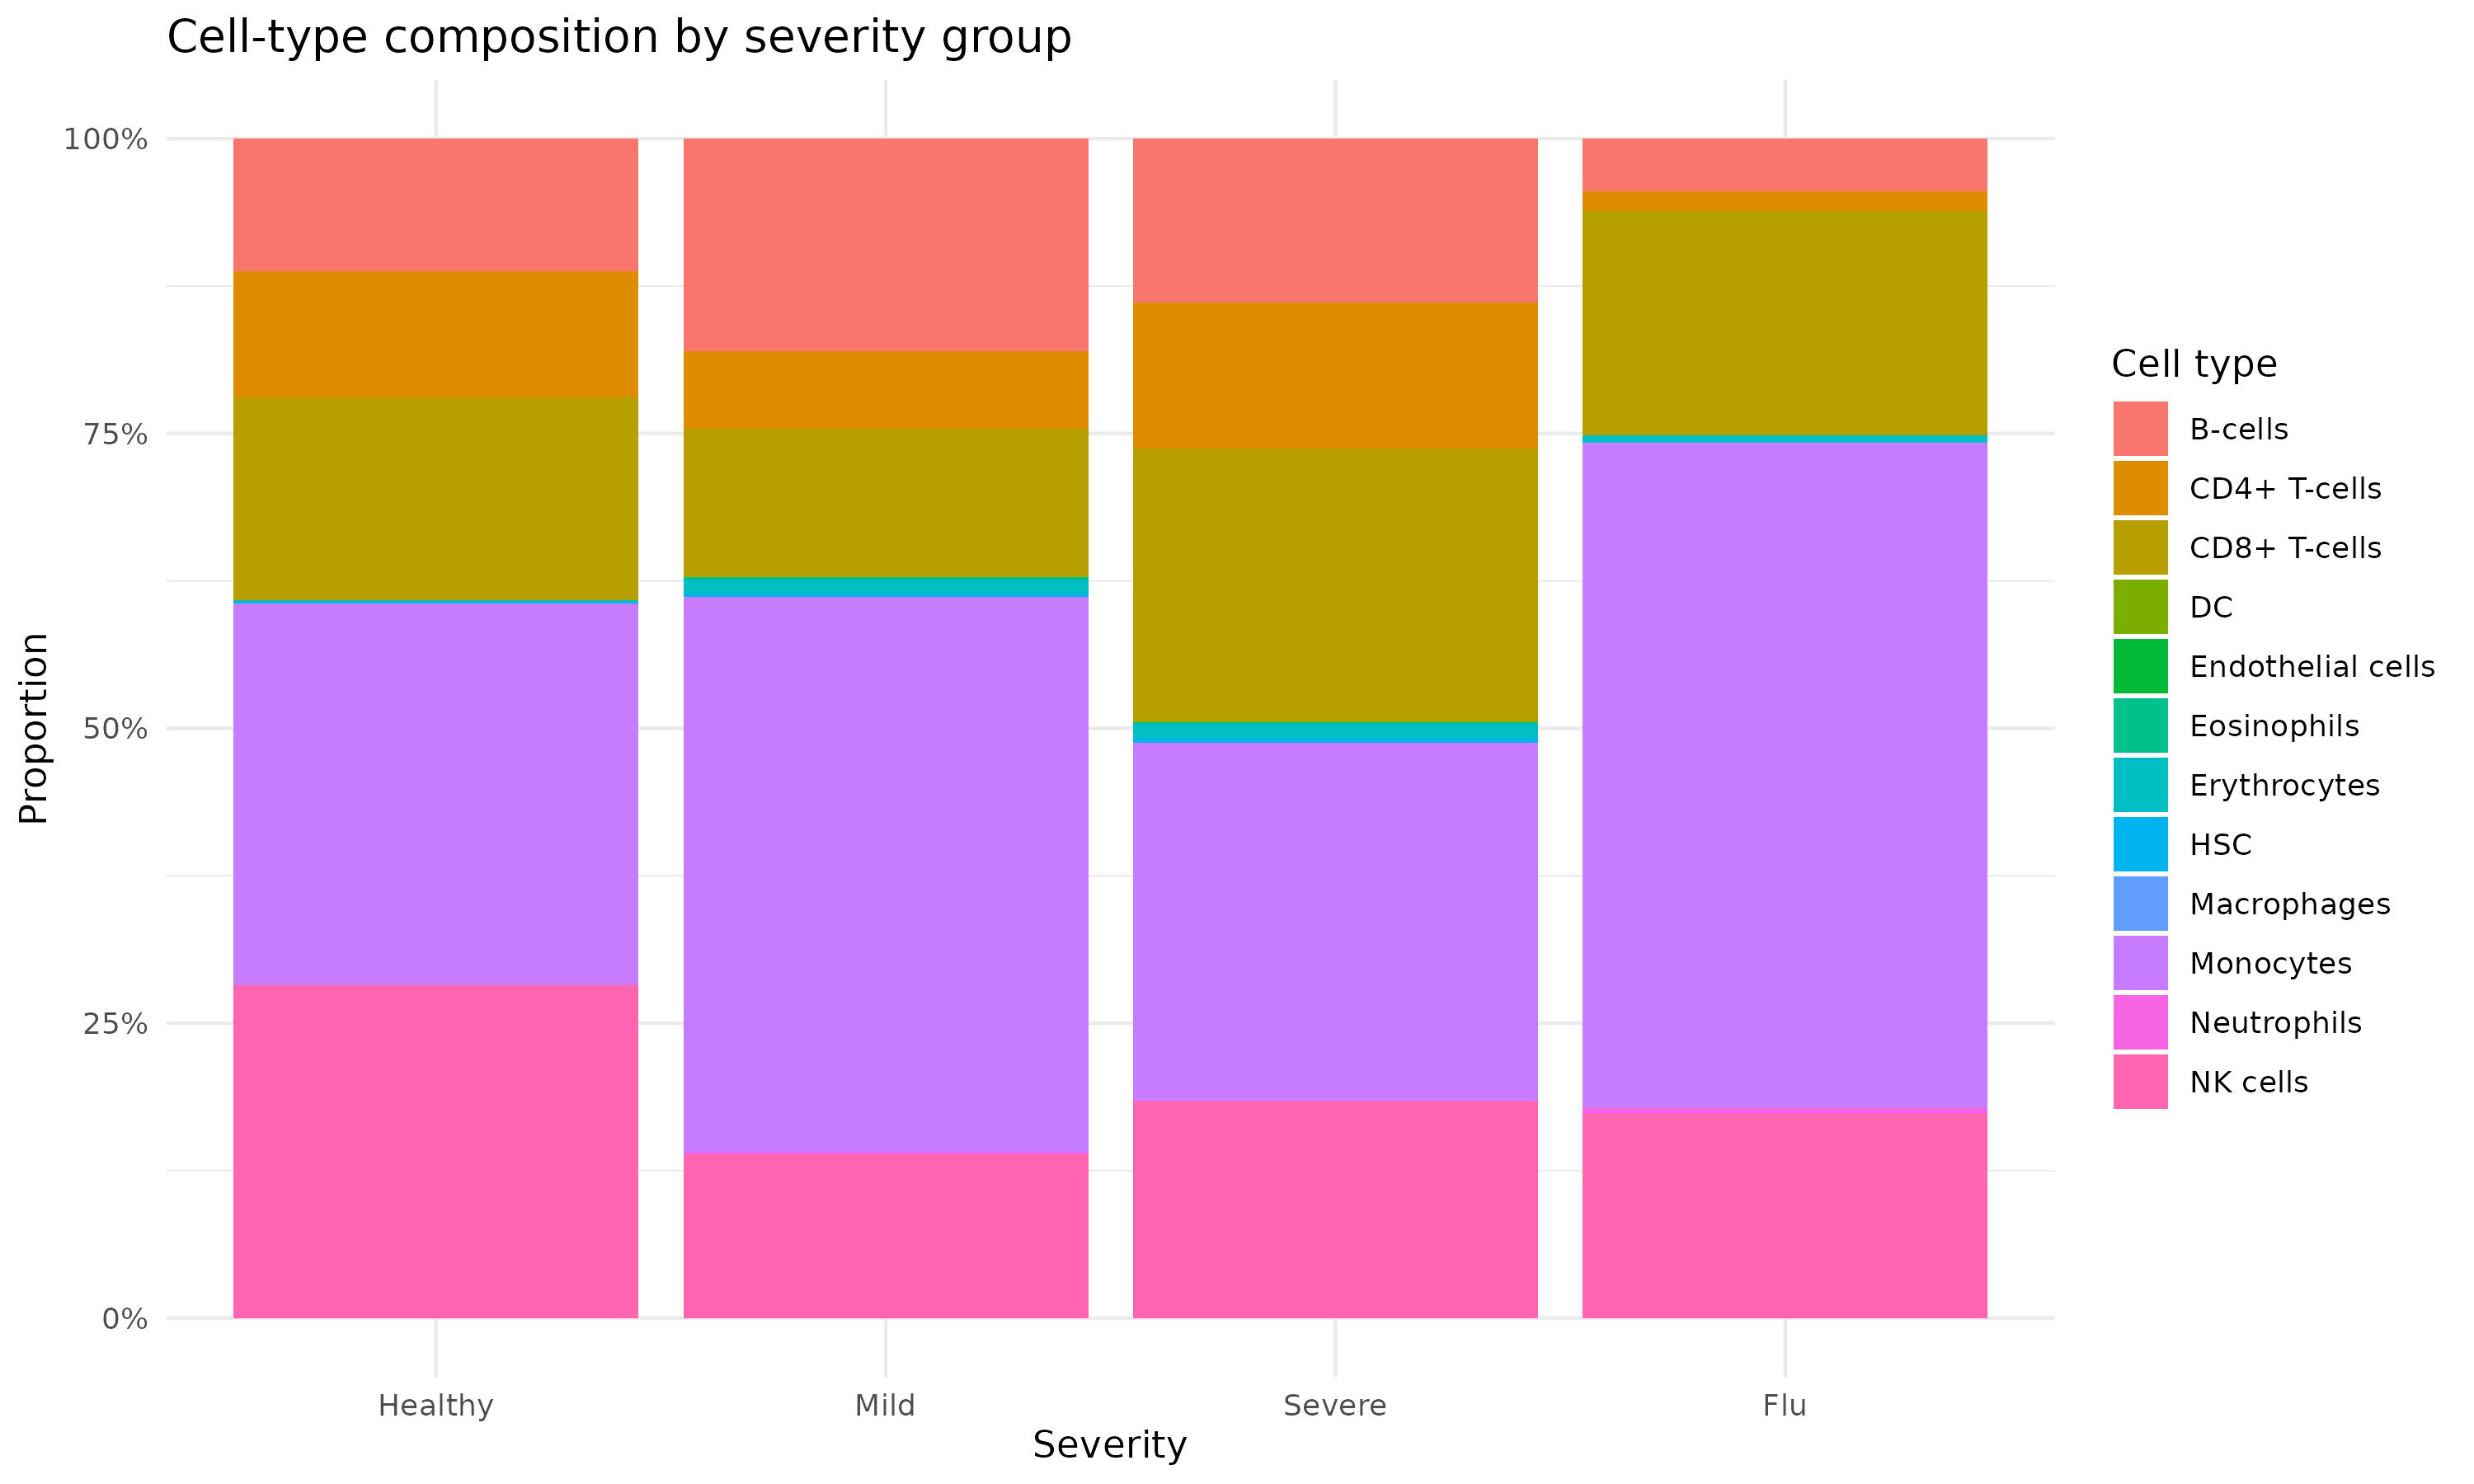
\includegraphics[width=0.9\textwidth]{plots/phase4/phase4_composition_barplot.png}
\end{center}

The stacked barplot converts the visual impression from the UMAP into exact
proportions. Each bar sums to 100\%.

\begin{itemize}[nosep]
  \item \textbf{Monocytes (purple):} Healthy $\approx$35\%, Mild $\approx$35\%,
        Severe $\approx$50\%, Flu $\approx$75\%.
        There is a clear stepwise increase with severity, and Flu is more extreme
        than Severe COVID.
  \item \textbf{NK cells (hot pink):} Healthy $\approx$28\%, dropping to
        $\approx$20\% in Severe and remaining moderate in Flu.
  \item \textbf{CD4$^+$ T cells (orange):} Healthy $\approx$12\%, shrinking in
        Severe to $\approx$5\%. \textbf{CD4$^+$ T cell depletion} is one of the
        hallmarks of severe COVID-19; this plot confirms it directly.
  \item \textbf{CD8$^+$ T cells (olive):} More stable across conditions,
        but slightly depleted in Severe.
  \item \textbf{B cells (salmon):} small and relatively stable, consistent with
        B cell biology being less dramatically altered in acute COVID.
\end{itemize}

\textbf{Key message:} the blood composition is not static — severe COVID
reshapes the immune cell balance. Monocytes expand and fill the space left
by depleted T cells. This already suggests the blood in severe COVID is
in a qualitatively different state, motivating us to zoom in on those monocytes.

\subsection{Module scoring and co-activation analysis \small\normalfont\textit{(Steps 5–9)}}

With severity labels attached and monocytes isolated (21,385 cells),
we now measure how strongly each monocyte runs the antiviral (ISG) and
inflammatory (TNF/IL-1$\beta$) programs.

\subsubsection*{Step 9 — Violin plots of scores by severity}

\begin{center}
  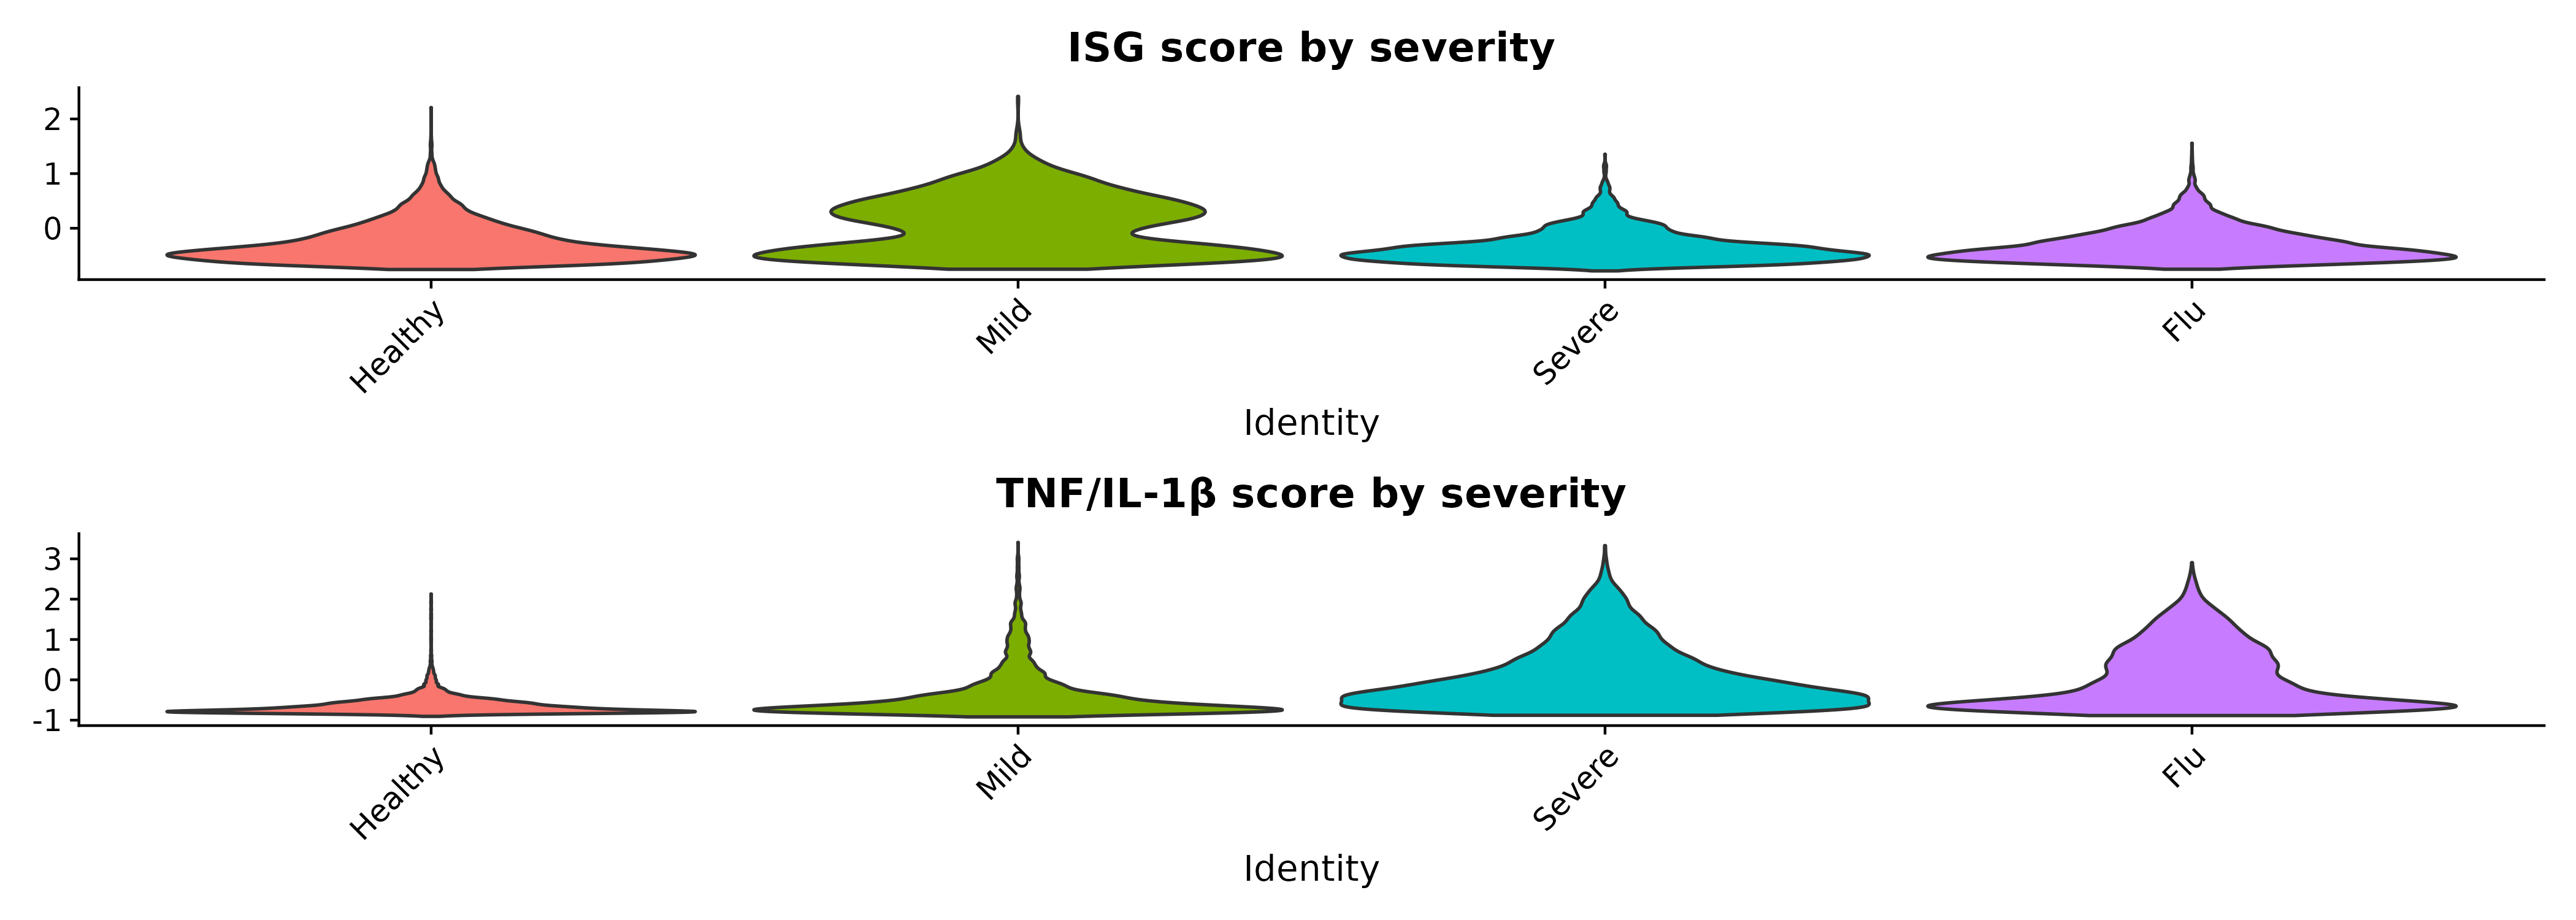
\includegraphics[width=\textwidth]{plots/phase4/phase4_violin_scores_severity.png}
\end{center}

Each violin shows the distribution of a module score across all monocytes in
one severity group. The x-axis is the score value; wider = more cells at that value.

\textit{Top panel — ISG score (antiviral program):}
\begin{itemize}[nosep]
  \item \textbf{Healthy:} tight, narrow violin centered near $-0.2$.
        The antiviral program is essentially off in healthy monocytes.
  \item \textbf{Mild Covid:} \textbf{bimodal} — the violin has two visible peaks,
        one near 0 and a second extending above 0.5.
        This is the most striking feature: in mild COVID, there are two distinct
        monocyte subpopulations — one with the ISG program partly on, one without.
        This could reflect donor heterogeneity or a genuine within-sample split
        between ISG-high and ISG-low monocytes.
  \item \textbf{Severe:} similar shape to Healthy — narrow, centered near 0.
        Somewhat counterintuitively, the ISG program is not broadly elevated
        at the cell level in Severe COVID monocytes.
  \item \textbf{Flu:} also narrow, similar to Healthy.
\end{itemize}

\textit{Bottom panel — TNF/IL-1$\beta$ score (inflammatory program):}
\begin{itemize}[nosep]
  \item \textbf{Healthy:} very tight at $-1$, essentially zero activity.
  \item \textbf{Mild:} slightly wider, still mostly low.
  \item \textbf{Severe:} \textbf{markedly broader} — the violin extends up to
        $\approx 3$ with a substantial body above 0. A large fraction of severe
        monocytes are actively running the inflammatory program.
        This is the clearest result so far: the TNF/IL-1$\beta$ program is
        specifically elevated in severe COVID monocytes at the cell level.
  \item \textbf{Flu:} also broader than Healthy, with a multi-bump shape
        suggesting multiple sub-states with varying inflammatory activity.
\end{itemize}

\subsubsection*{Step 7 — Co-activation scatter (the central plot)}

\begin{center}
  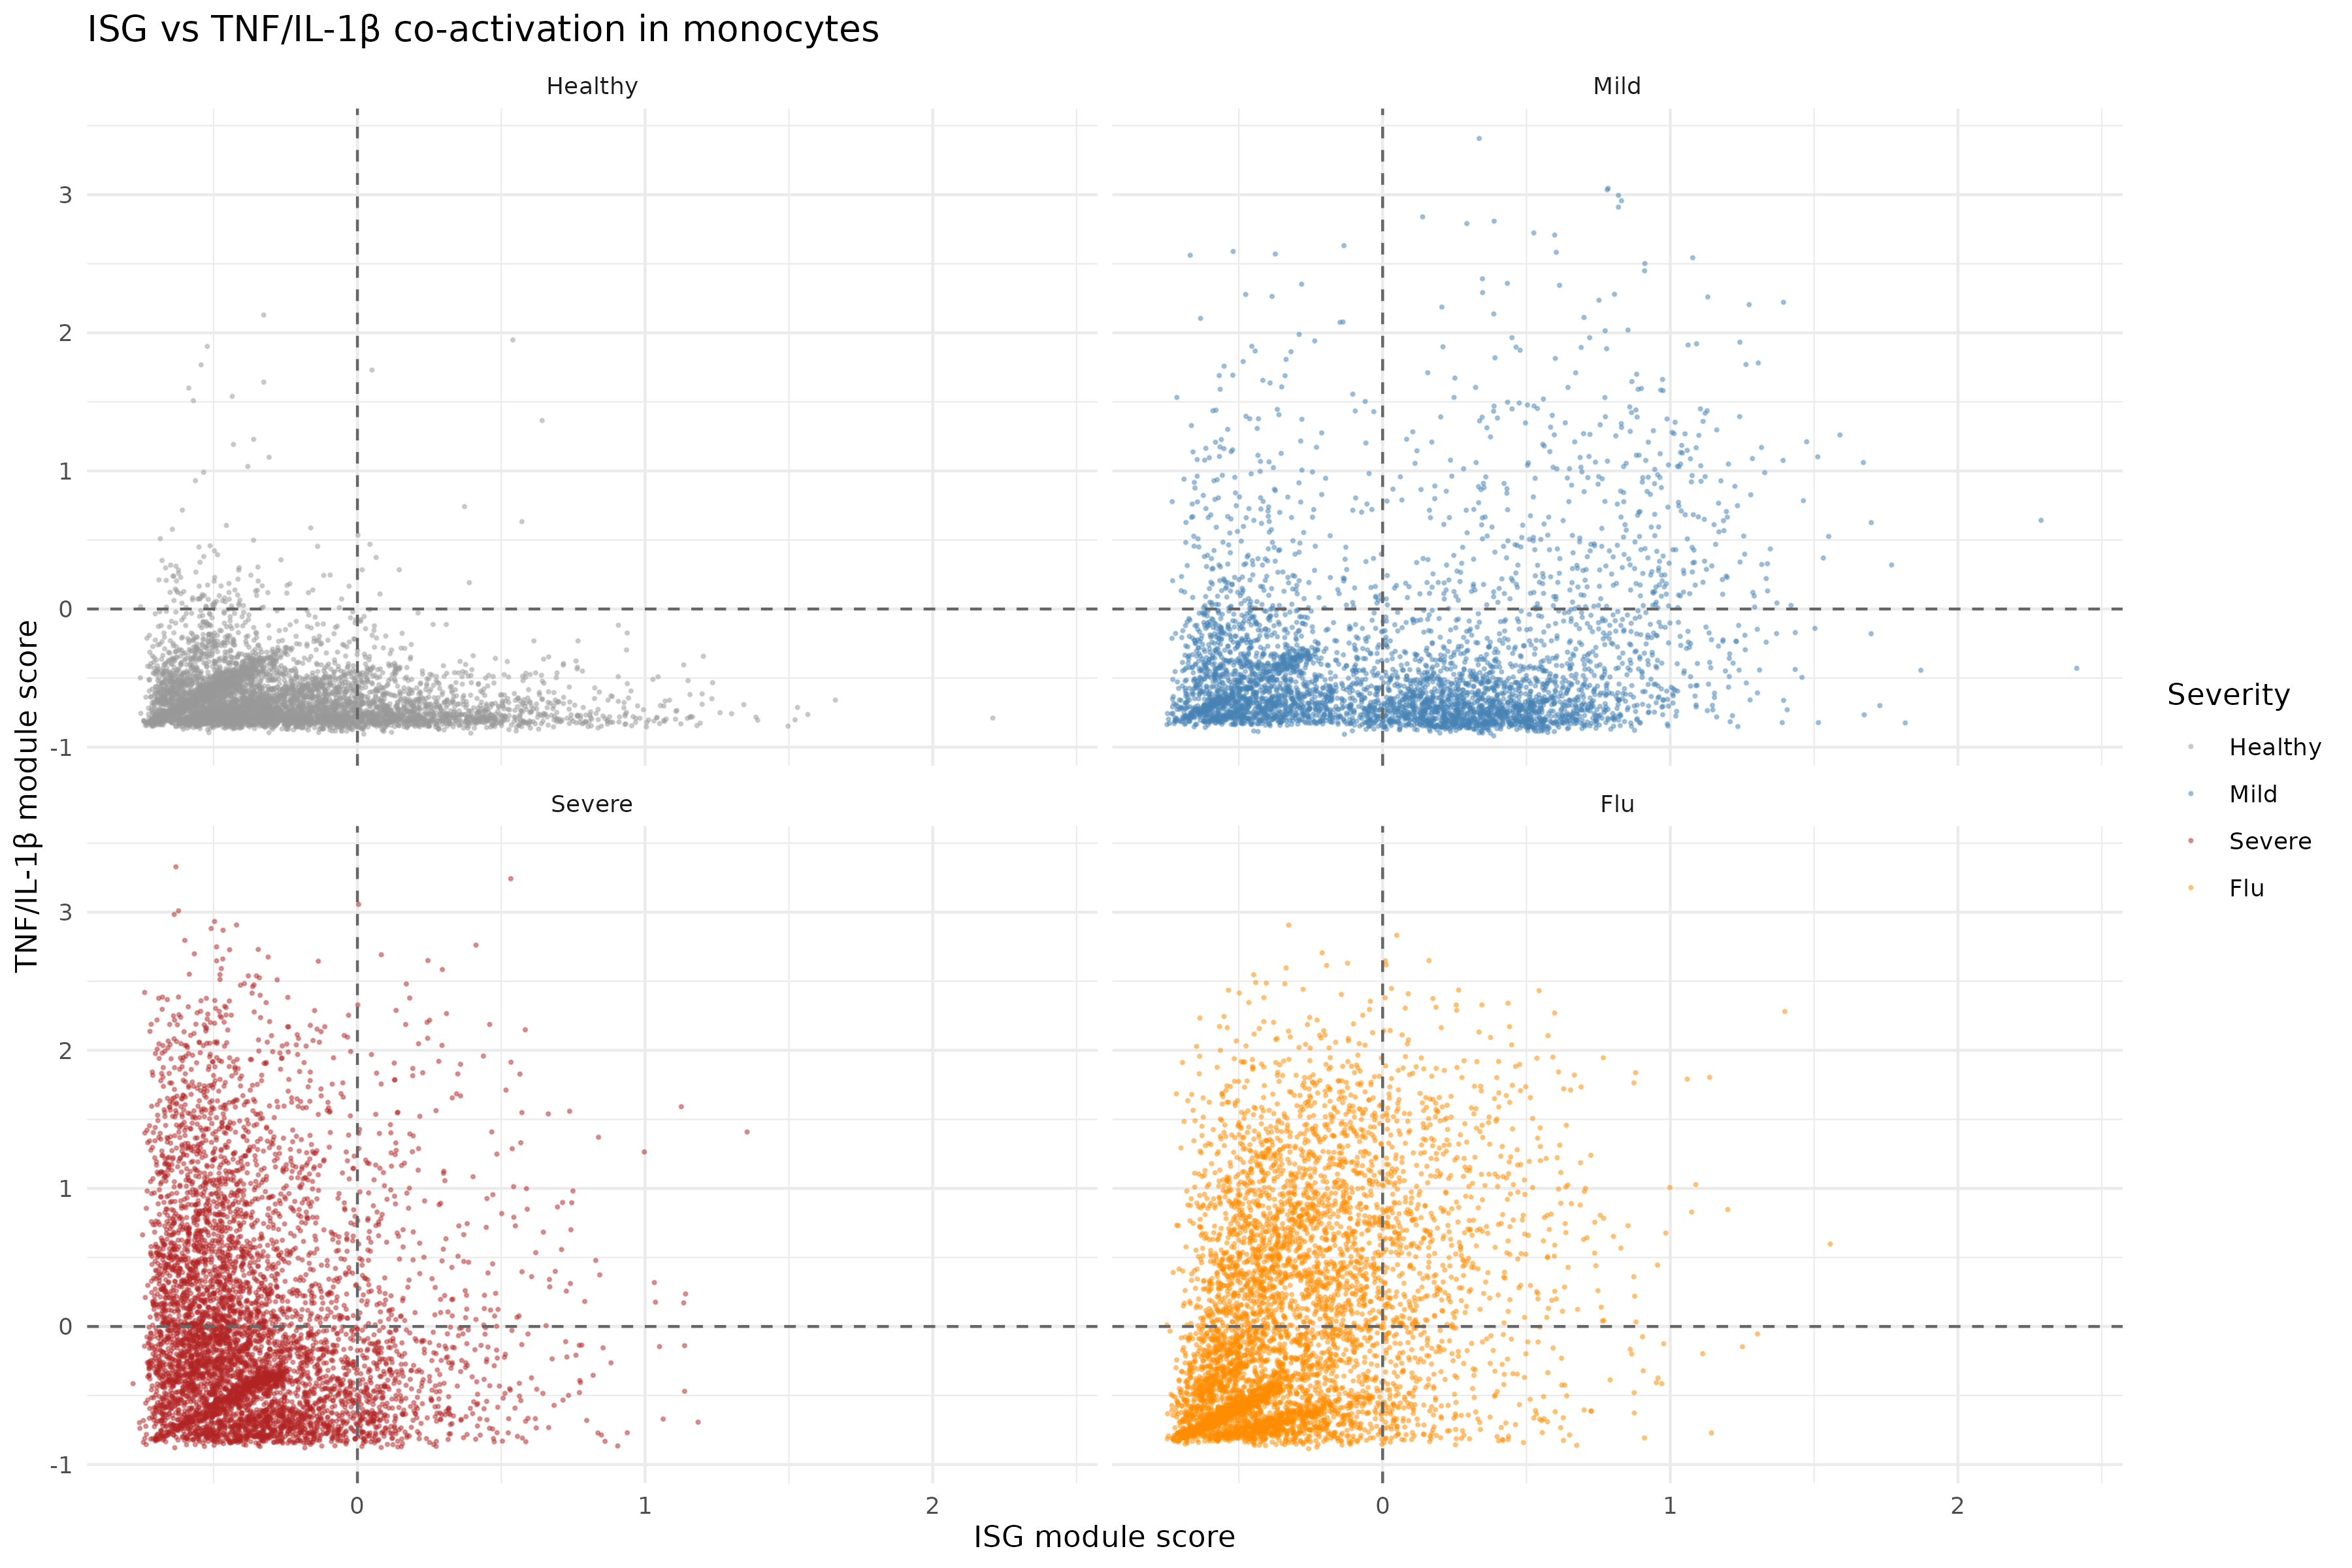
\includegraphics[width=\textwidth]{plots/phase4/phase4_coactivation_scatter.png}
\end{center}

This is the most important plot in Phase 4.
Each dot is one monocyte. The x-axis is its ISG score; the y-axis is its
TNF/IL-1$\beta$ score. The dashed lines at $x = 0$ and $y = 0$ divide
the plot into four quadrants:

\begin{center}
\begin{tabular}{@{}p{3cm}p{5.5cm}p{4cm}@{}}
\toprule
\textbf{Quadrant} & \textbf{meaning} & \textbf{label} \\
\midrule
Top-right    & both programs on  & \textbf{co-activated} \\
Top-left     & only inflammation on & inflamed, not antiviral \\
Bottom-right & only ISG on       & antiviral, not inflamed \\
Bottom-left  & both programs off & resting \\
\bottomrule
\end{tabular}
\end{center}

\begin{itemize}[nosep]
  \item \textbf{Healthy:} cells cluster tightly in the bottom-left. Both programs
        are off. This is the expected resting state.
  \item \textbf{Mild:} cells spread widely in all four directions, including the
        top-right (co-activated) quadrant. There is a visible cloud of blue dots
        with both ISG $> 0$ and TNF/IL-1$\beta > 0$.
        This was partly unexpected — mild COVID shows the most ISG activity
        at the cell level (consistent with the bimodal violin above).
  \item \textbf{Severe:} the cell cloud shifts \textit{upward and to the left}.
        Many red cells are in the top-left (high TNF/IL-1$\beta$, low ISG) —
        these are cells running pure inflammation without antiviral response.
        Fewer cells are in the top-right compared to Mild, but the ones
        that are there (co-activated) are more extreme in their TNF/IL-1$\beta$
        scores (reaching $y \approx 3$).
  \item \textbf{Flu:} similar pattern to Severe — a large upper-left mass,
        with a subset in the top-right.
\end{itemize}

\textbf{Interpretation:} the co-activated state (top-right) is present in all
conditions except Healthy, but the \textit{nature} of the activation differs:
Mild COVID monocytes tend toward ISG-high states; Severe COVID monocytes
tend toward TNF/IL-1$\beta$-high states. The worst outcomes (severe disease)
are associated with a shift toward unchecked inflammation rather than
ISG-based antiviral defense.

\subsection{Donor-level comparison \small\normalfont\textit{(Steps 10–12)}}

Cell-level analysis reflects thousands of cells per condition, but cells from
the same donor are not independent. The \textbf{correct unit of comparison
for between-condition statistics is the donor}, not the individual cell.
Each donor's monocytes are averaged into one summary score.

\subsubsection*{Step 12 — Donor-level boxplots}

\begin{center}
  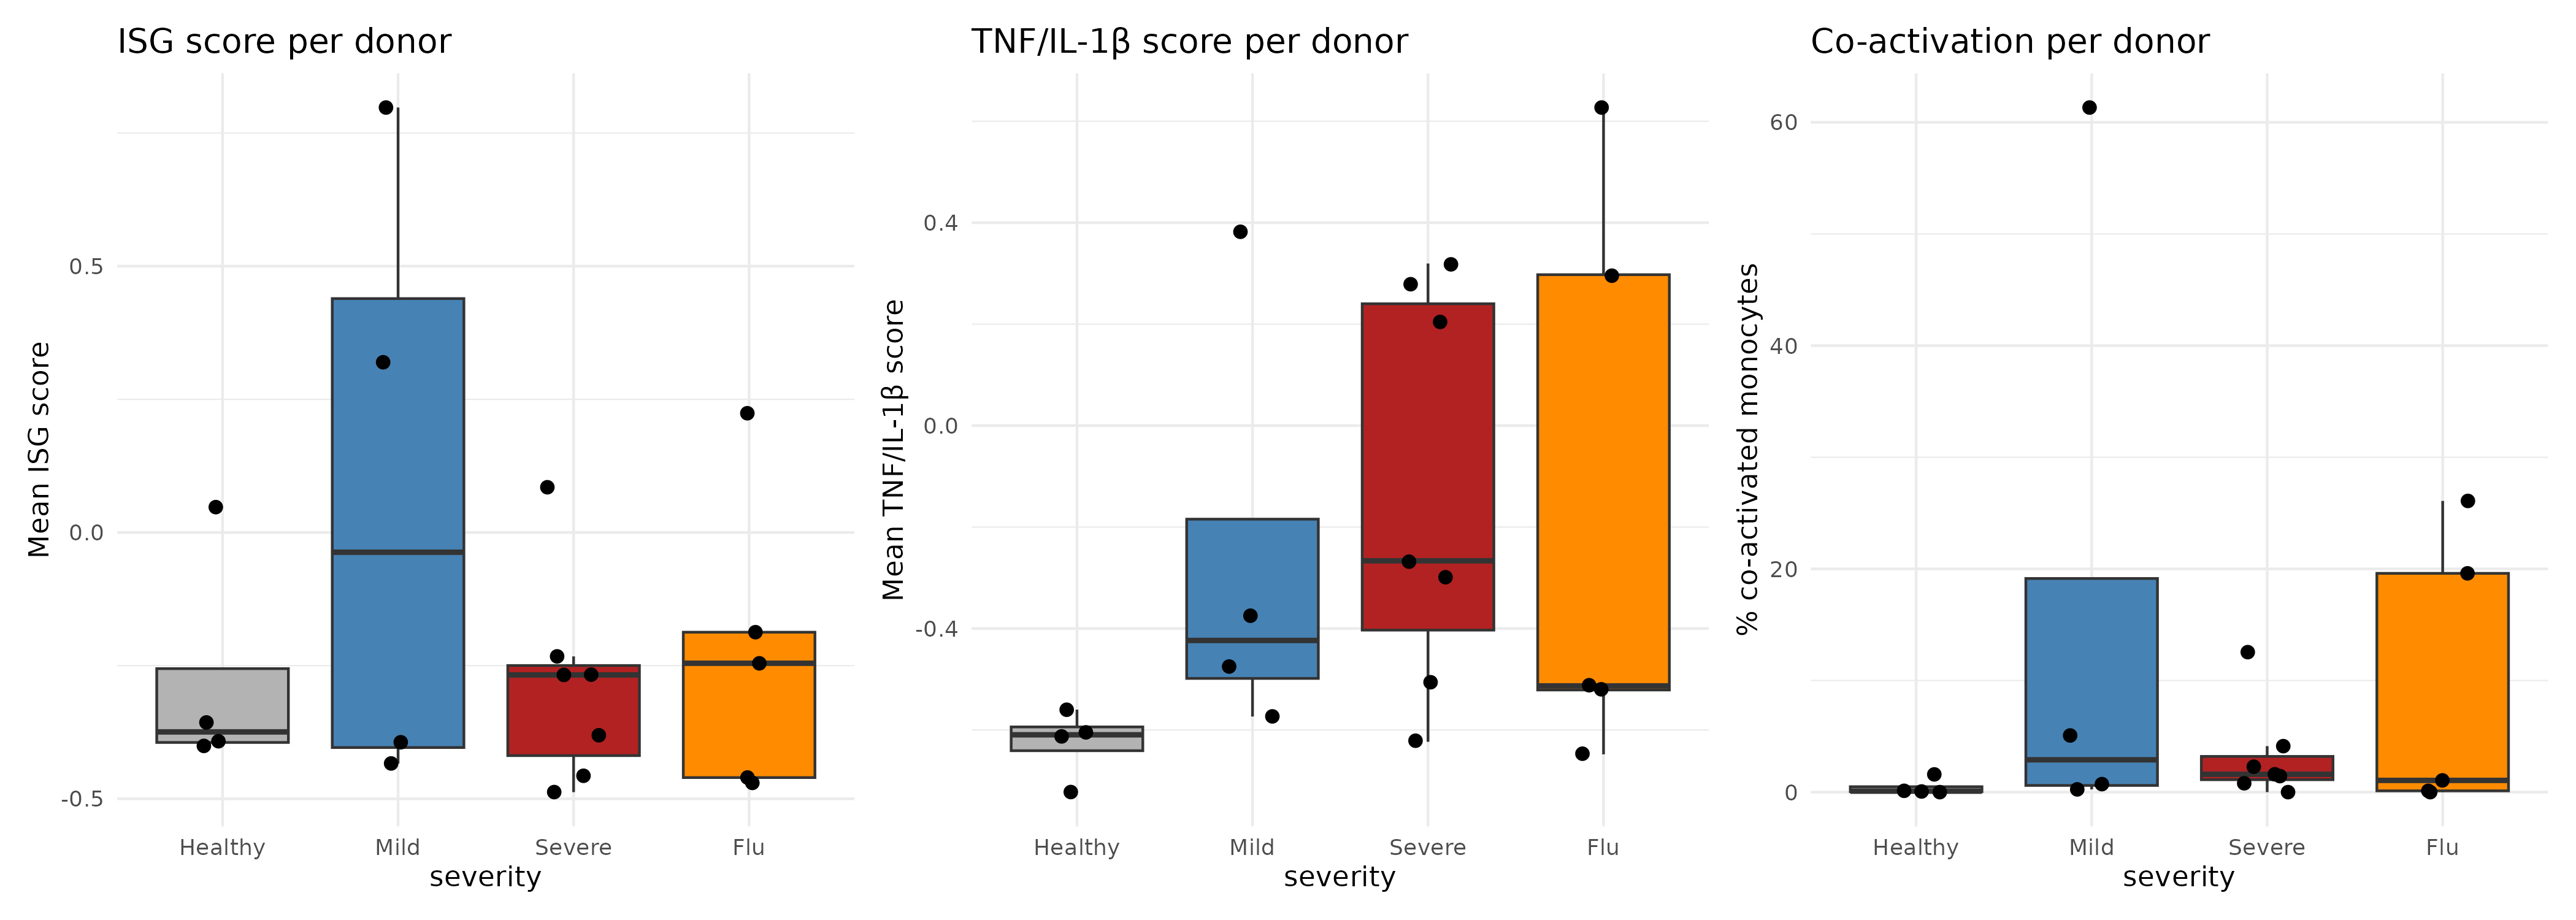
\includegraphics[width=\textwidth]{plots/phase4/phase4_donor_boxplots.png}
\end{center}

Each dot is one donor; the box shows the interquartile range.

\textit{Left — ISG score per donor:}
\begin{itemize}[nosep]
  \item Mild COVID has the highest median ISG score among donors,
        with one outlier donor reaching $\approx 0.9$.
  \item Severe COVID has a \textit{lower} mean ISG score than Mild — despite
        being more clinically severe. The ISG program is actually more
        consistently elevated in mild disease at the donor level.
  \item Healthy donors are tightly clustered near $-0.5$.
  \item Flu falls between Healthy and Mild.
\end{itemize}

\textit{Middle — TNF/IL-1$\beta$ score per donor:}
\begin{itemize}[nosep]
  \item Healthy donors cluster tightly near $-0.6$ — essentially silent.
  \item Mild shows modest elevation.
  \item \textbf{Severe and Flu} have the highest medians and widest spread.
        Several Severe donors have scores above 0, and the best-separated
        donors reach $\approx +0.4$.
  \item This confirms the violin finding: the inflammatory program is elevated
        in severe/flu conditions at the donor level too.
\end{itemize}

\textit{Right — Co-activation \% per donor:}
\begin{itemize}[nosep]
  \item \textbf{Healthy:} 3 of 4 donors have essentially 0\% co-activated
        monocytes. The resting state is clean.
  \item \textbf{Mild:} moderate — median around 5\%, but with one outlier
        donor near 20\%.
  \item \textbf{Severe:} \textbf{highest variance}. Most donors are low,
        but one outlier donor has \textit{61\% co-activated monocytes} — an
        extraordinary proportion. This donor appears to have a genuinely unusual
        immune state where both programs are simultaneously on in the majority
        of circulating monocytes.
  \item \textbf{Flu:} similar pattern to Severe, with one very high outlier.
\end{itemize}

\textbf{Statistical tests (Wilcoxon rank-sum, Mild vs.\ Severe, donor-level):}
The wide variance within Severe COVID — driven by donor heterogeneity — means
that no comparison reaches clear statistical significance with only 4--7 donors
per group. This is a known limitation of the dataset (small N) and does not
negate the directional findings visible in the plots.

\subsection{Differential expression and volcano plot \small\normalfont\textit{(Steps 13–14)}}

The module scores tell us about the two specific programs we defined.
But are there other genes that change in severe COVID monocytes?
\texttt{FindMarkers()} compares all genes between Severe Covid monocytes and
Healthy monocytes systematically, without pre-specifying any gene list.

\textbf{Result:} 3,269 differentially expressed genes between Severe and Healthy
monocytes (Wilcoxon test, $p_\text{adj} < 0.05$, $\log_2 \text{FC} > 0.25$).
This large number confirms that monocytes are dramatically changed in severe disease.

\subsubsection*{Step 14 — Volcano plot}

\begin{center}
  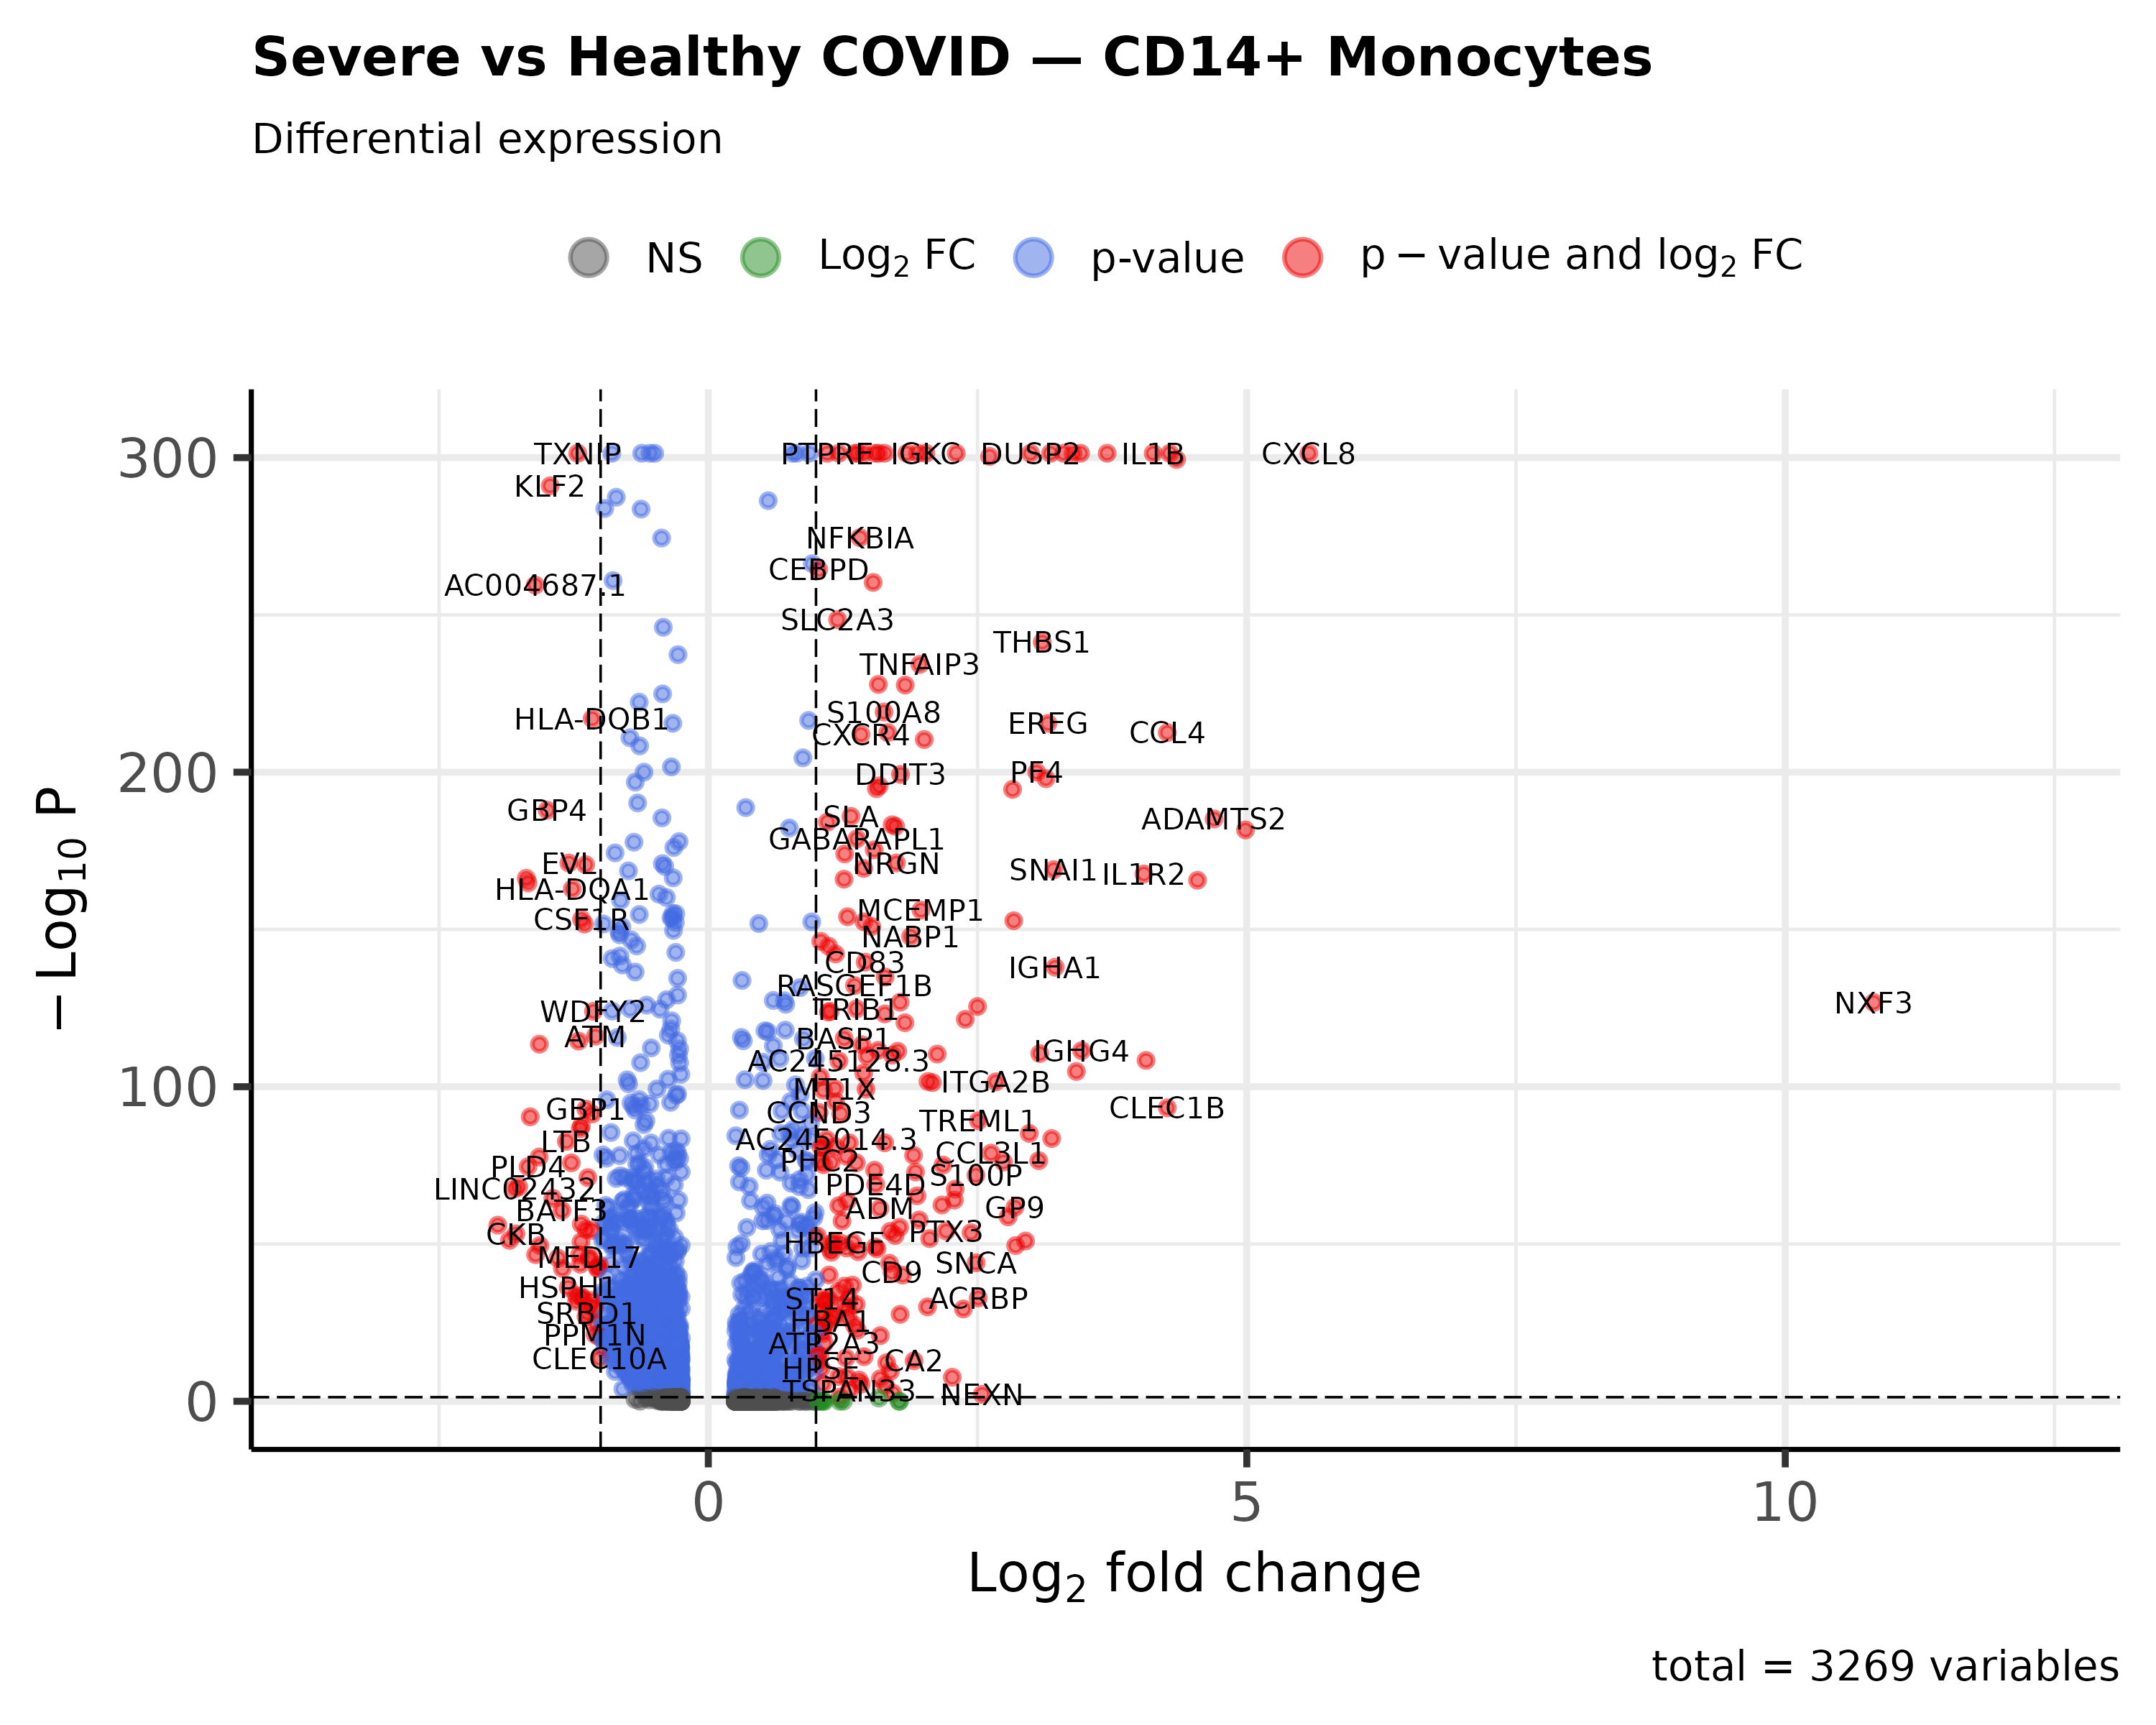
\includegraphics[width=0.95\textwidth]{plots/phase4/phase4_volcano_monocyte_DE.png}
\end{center}

The volcano plots each gene as a point.
x-axis = $\log_2$ fold-change (how much more or less expressed in Severe vs Healthy).
y-axis = $-\log_{10}$ adjusted p-value (higher = more significant).
\textbf{Red} = significant both in fold-change and p-value.
\textbf{Blue} = significant in p-value only. \textbf{Grey} = not significant.

\textit{Top upregulated genes in Severe monocytes (red, top-right):}
\begin{itemize}[nosep]
  \item \textbf{IL1B} ($\log_2$FC $\approx 5$, $-\log P \approx 300$) — the strongest
        single result. IL-1$\beta$ is the core cytokine of the monocyte inflammasome.
        Its extreme upregulation in severe COVID monocytes directly confirms
        the TNF/IL-1$\beta$ module finding.
  \item \textbf{CXCL8} ($\log_2$FC $\approx 5$) — interleukin-8, a key neutrophil
        recruiter. High CXCL8 from monocytes drives neutrophil-mediated lung
        damage in severe COVID.
  \item \textbf{CCL4, EREG, IL1R2, ADAMTS2} — additional inflammatory mediators
        and receptors upregulated in the severe monocyte state.
  \item \textbf{NFKBIA, TNFAIP3} — feedback inhibitors of NF-$\kappa$B signaling.
        Their upregulation alongside IL1B/CXCL8 indicates the cell is trying to
        brake its own activation — a hallmark of a chronically activated state.
  \item \textbf{NXF3} (far right, $\log_2$FC $\approx 11$) — an RNA export factor.
        This outlier is not an established COVID gene and may warrant follow-up.
\end{itemize}

\textit{Top downregulated genes in Severe monocytes (left side):}
\begin{itemize}[nosep]
  \item \textbf{TXNIP} (most significantly downregulated) — thioredoxin-interacting
        protein, a negative regulator of oxidative stress. Its loss means a loss
        of a brake on reactive oxygen species production.
  \item \textbf{KLF2} — a transcription factor that keeps monocytes in a
        ``patrolling'' anti-inflammatory state. Its downregulation is consistent
        with monocytes losing their homeostatic identity.
  \item \textbf{HLA-DQA1, HLA-DQB1} — MHC class II molecules required for
        antigen presentation. Their downregulation is a well-documented feature
        of severe COVID monocytes and is called \textbf{monocyte deactivation} or
        \textbf{immunoparalysis} — the monocytes become pro-inflammatory but lose
        their ability to present antigens to T cells.
  \item \textbf{GBP4, CSF1R} — innate immune regulators further lost in severe disease.
\end{itemize}

\textbf{Overall picture from this volcano:} severe COVID monocytes gain a massive
inflammatory output (IL-1$\beta$, CXCL8, CCL4) while simultaneously losing their
homeostatic and antigen-presenting identity (KLF2, HLA-DQ, TXNIP). This is not
a simple ``activation'' — it is a pathological reprogramming.

\subsection{Phase 4 conclusion}

Phase 4 directly tests the central hypothesis of the project at the single-cell level.
The key findings are:

\begin{enumerate}[nosep]
  \item \textbf{Monocytes expand with severity.}
        From $\approx$35\% in Healthy to $\approx$50\% in Severe and $\approx$75\%
        in Flu. CD4$^+$ T cells deplete in parallel — this is the emergency myeloid
        shift typical of severe acute infection.

  \item \textbf{The inflammatory program is elevated in Severe monocytes.}
        TNF/IL-1$\beta$ scores are higher in Severe COVID donors than in Healthy
        or Mild, at both the cell level (violin) and donor level (boxplot).

  \item \textbf{The antiviral (ISG) program peaks in Mild COVID, not Severe.}
        This is counterintuitive but important: it suggests that in mild disease,
        the immune system successfully mounts an interferon response; in severe
        disease, the response shifts toward unchecked inflammation, with ISG
        activity not sustaining.

  \item \textbf{Co-activated monocytes exist and are enriched in Severe COVID.}
        The top-right quadrant (both programs active) is populated in all infected
        conditions but virtually absent in Healthy. Some Severe donors have
        extraordinarily high co-activation rates ($>$60\%).

  \item \textbf{3,269 DE genes confirm broad monocyte reprogramming.}
        The volcanic eruption of IL1B and CXCL8 combined with the loss of HLA-DQ
        and KLF2 paints a cell that is simultaneously hyper-inflammatory and
        functionally impaired.
\end{enumerate}

\textbf{Limitation:} with only 4--7 donors per group, within-group variance is high 
and formal statistical tests lack power. The directional trends are consistent
across all analyses, but confirmatory evidence in a larger or independent cohort
is essential. That is exactly what Phase 5 does.

% ─────────────────────────────────────────────
\section{Phase 5 — Replication on GSE150861}
% ─────────────────────────────────────────────

\subsection{Phase 5 overview — the big picture}

\textbf{Phase 4 found the co-activated state. Phase 5 checks whether it is real
by looking for it in a completely different dataset.}

A finding in one dataset could be a fluke — a property of those specific donors,
that lab's protocol, or random noise. \textbf{Replication in an independent
dataset is the strongest evidence} we can produce that a biological signal
is genuine.

GSE150861 (Guo et al., \textit{Nat Commun} 2020) is the ideal replication
dataset because it differs from GSE149689 in almost every way that matters:
different patients, different lab, different country, different sequencing run —
but the same disease (severe COVID-19) and the same cell type (blood monocytes).
It also adds something new: \textbf{Tocilizumab treatment and time-series sampling
(Day 1, Day 5, Day 7)}, which lets us ask whether the co-activated state
\textit{changes} during treatment.

The exact same analysis pipeline is rerun from scratch on this new data:
same QC thresholds, same normalization, same 20 PCs, same resolution 0.5,
same ISG and TNF/IL-1$\beta$ gene lists. No parameters are changed.

\subsection{Dataset and QC \small\normalfont\textit{(Steps 2–4)}}

GSE150861 contains PBMCs from \textbf{2 severe COVID-19 patients (P1, P2)},
each sampled at \textbf{Day 1, Day 5, and Day 7} of Tocilizumab treatment.
Tocilizumab is an antibody that blocks the IL-6 receptor, used to dampen
the cytokine storm in severe COVID-19.

\textbf{Dataset scale:}
\begin{itemize}[nosep]
  \item 6 samples total (2 patients $\times$ 3 time points).
  \item Before QC: $\sim$16,000 barcodes.
  \item After QC (nFeature $>$ 200, $<$ 5,000; percent.mt $<$ 20\%): retained cells
        cover all six patient-day combinations with reasonable representation.
\end{itemize}

\subsubsection*{Step 4a — QC violin plots}

\begin{center}
  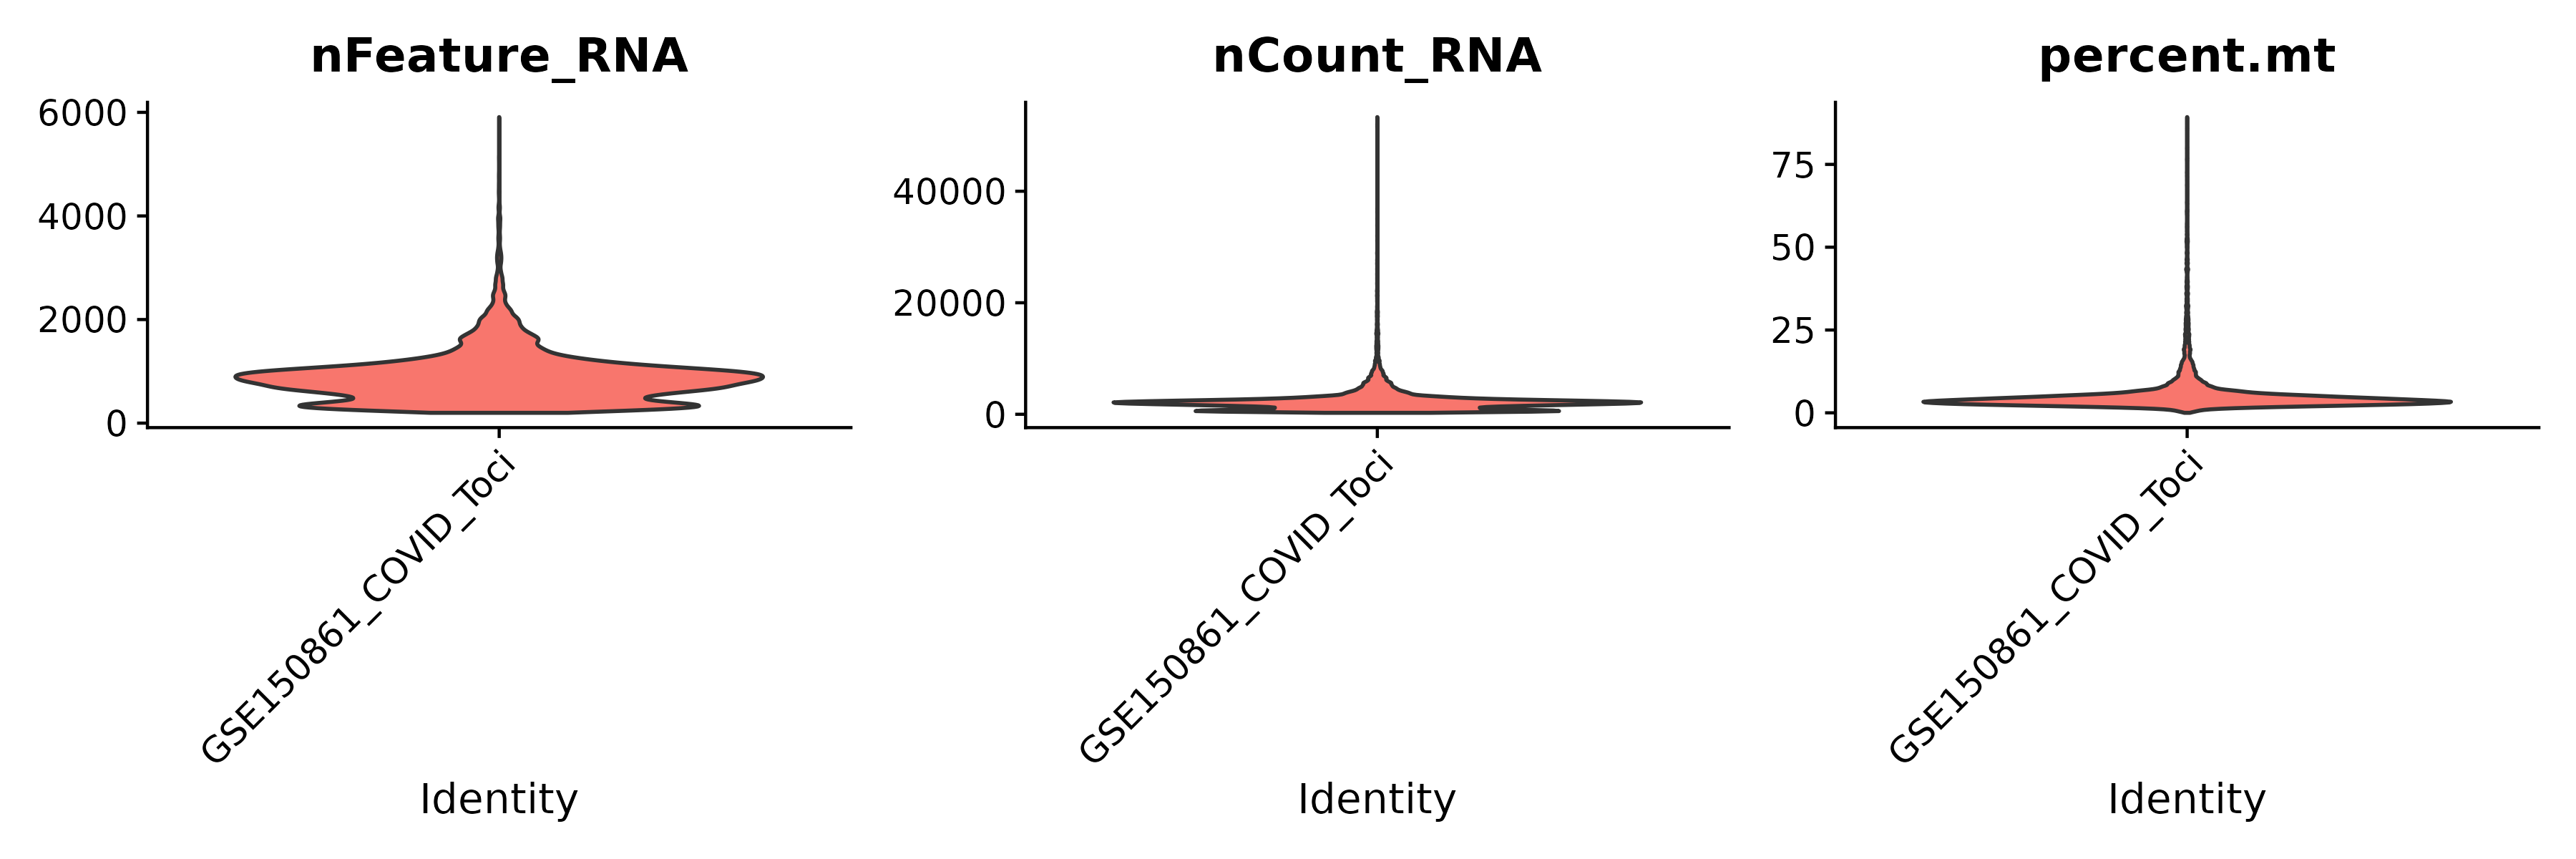
\includegraphics[width=\textwidth]{plots/phase5/phase5_qc_violin.png}
\end{center}

The three panels show nFeature\_RNA, nCount\_RNA, and percent.mt for the
full dataset (all 6 batches pooled). The shape is similar to Phase 1:
\begin{itemize}[nosep]
  \item \textbf{nFeature\_RNA}: a large body of cells between 500 and 3,000
        genes, with a spike up to 6,000 (doublet candidates at the top).
        The main mass looks healthy.
  \item \textbf{nCount\_RNA}: most cells fall below 10,000 UMIs, with a tail
        reaching $\sim$40,000. Similar to Phase 1, a few high-count outliers
        are present.
  \item \textbf{percent.mt}: the violin extends up to $\sim$80\% with a thin
        spike, but the bulk sits below 20\%. This dataset has fewer high-mito
        cells than Phase 1 GSE149689, which had nearly 25\% of cells above
        the 20\% threshold.
\end{itemize}

\subsubsection*{Step 4b — QC scatter plots}

\begin{center}
  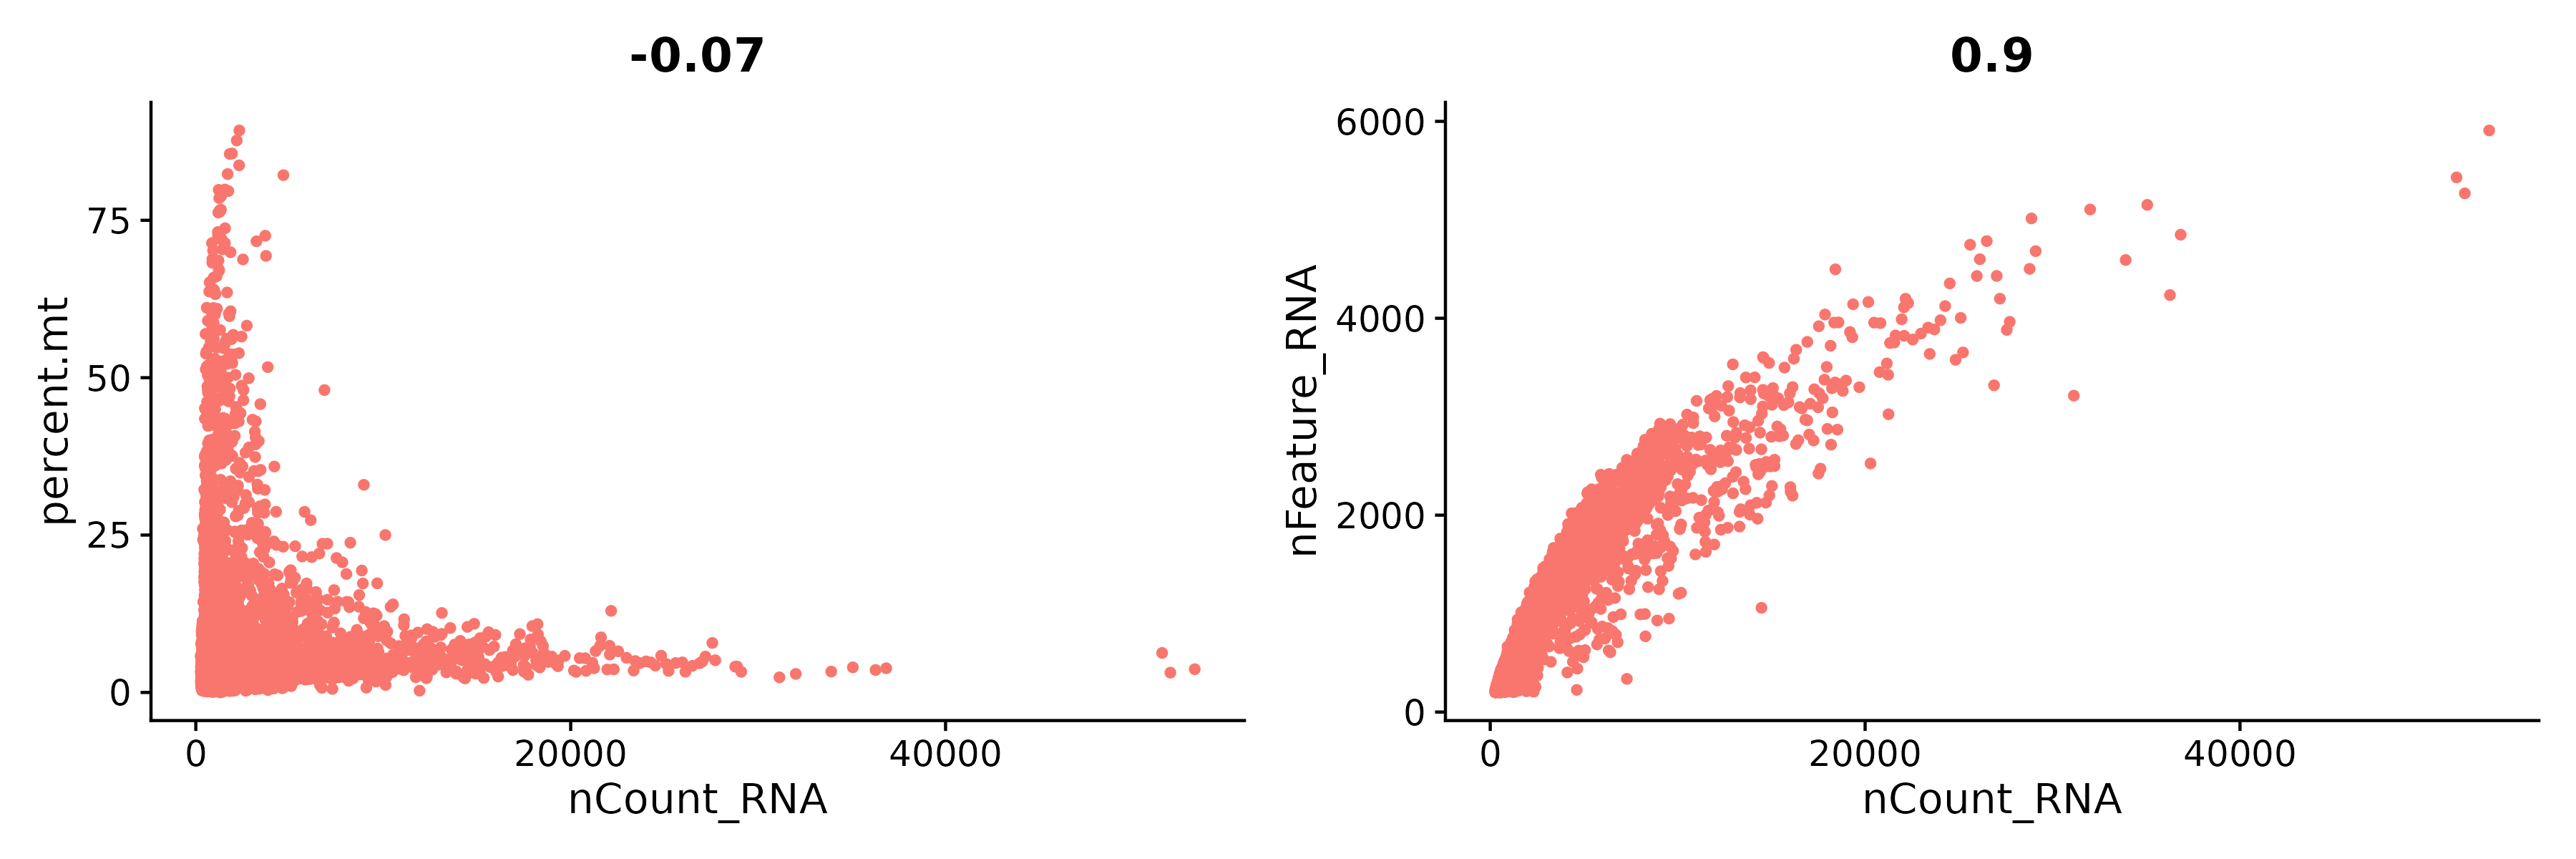
\includegraphics[width=0.95\textwidth]{plots/phase5/phase5_qc_scatter.png}
\end{center}

\begin{itemize}[nosep]
  \item \textbf{Left (correlation $= -0.07$): nCount\_RNA vs percent.mt.}
        The correlation is essentially zero — unlike Phase 1 where low-count
        cells had dramatically elevated mito percentages, here the mito
        percentage is flat across the count range. This suggests the cells
        in this dataset are generally healthier, with fewer severely stressed
        low-count cells in the capture.
  \item \textbf{Right (correlation $= 0.9$): nCount\_RNA vs nFeature\_RNA.}
        The tight upward curve (Pearson $r = 0.9$) is identical in shape to
        Phase 1: more counts means more distinct genes detected, with
        diminishing returns at higher counts. The curve is clean with no
        anomalous off-diagonal blobs.
\end{itemize}

\subsection{Normalization, PCA, and choosing the number of PCs \small\normalfont\textit{(Step 5–6)}}

The same normalization pipeline as Phase 2 is applied (LogNormalize,
3,000 variable features, scale and regress out percent.mt).

\subsubsection*{Step 6 — Elbow plot}

\begin{center}
  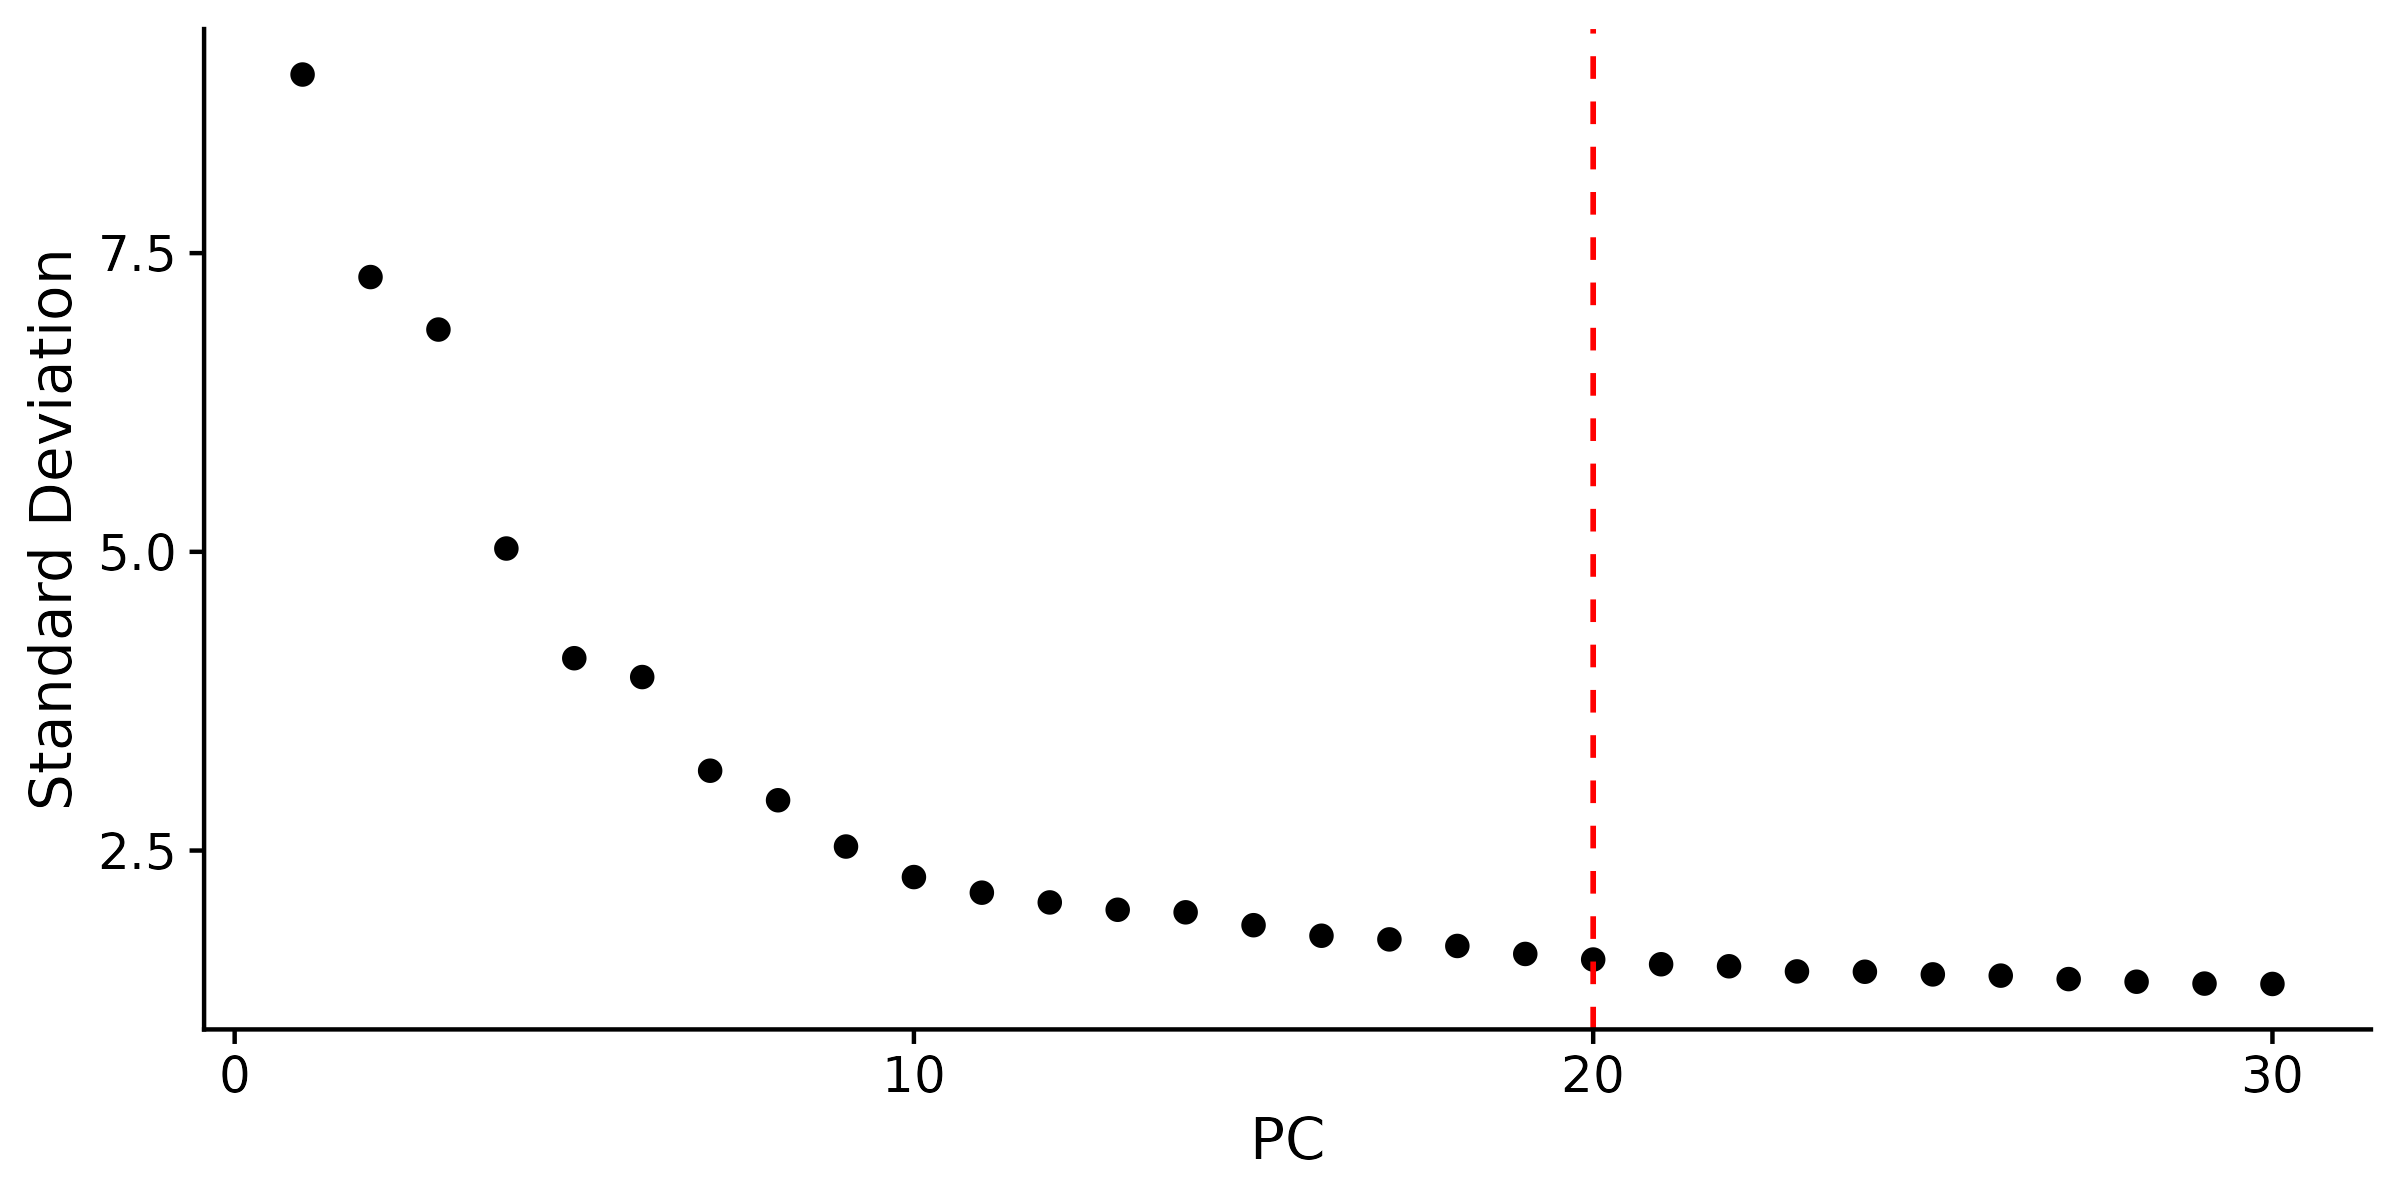
\includegraphics[width=0.85\textwidth]{plots/phase5/phase5_elbow_plot.png}
\end{center}

The elbow plot of this independent dataset is \textbf{strikingly similar
to Phase 2}:
\begin{itemize}[nosep]
  \item PC1 dominates with std $\approx 8$ (slightly lower than Phase 1's 14,
        reflecting the smaller and more homogeneous dataset — only severe COVID
        patients, no healthy donors).
  \item PCs 2--4 gradually decline from $\approx 7$ to $\approx 5$.
  \item The curve flattens to a plateau around PC\,15--20.
  \item The red dashed line at PC\,20 sits right at the beginning of the
        flat noise floor.
\end{itemize}

\textbf{Decision: keep 20 PCs} — the same as Phase 2.
The fact that an independent dataset with different patients and a different
cell composition leads to the same optimal PC cutoff validates the Phase 2
choice rather than being a coincidence.

\subsection{UMAP and clustering \small\normalfont\textit{(Step 6, continued)}}

\subsubsection*{Step 6 — UMAP overview (clusters, patient, time point)}

\begin{center}
  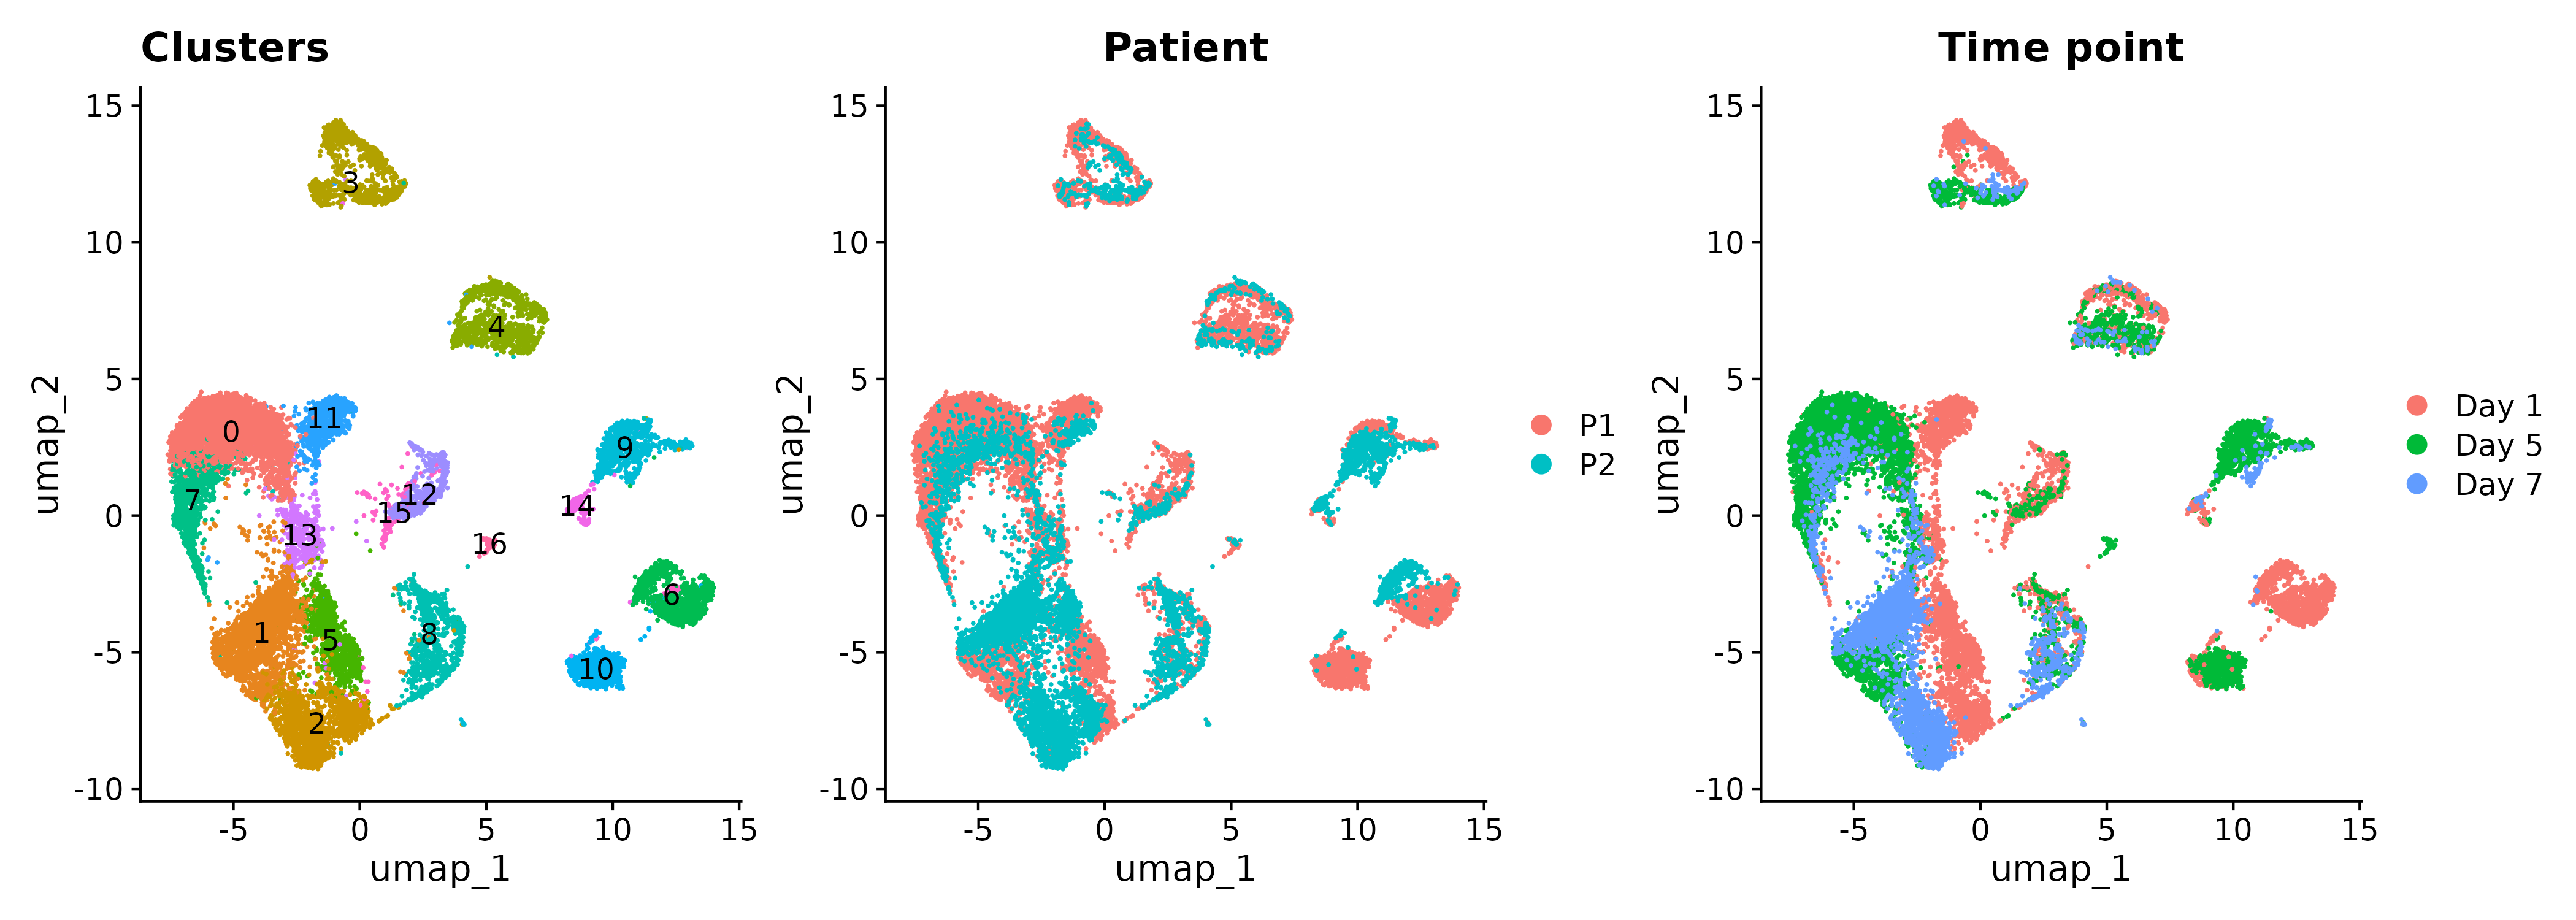
\includegraphics[width=\textwidth]{plots/phase5/phase5_umap_overview.png}
\end{center}

Three views of the same UMAP: coloured by cluster (left), by patient (middle),
and by time point (right).

\begin{itemize}[nosep]
  \item \textbf{Clusters (left):} 17 clusters at resolution 0.5. The topology
        is recognizable: a large left lymphoid continent (T/NK cells),
        an isolated monocyte mass on the right (clusters 6, 10, 14, 16),
        two isolated B cell blobs at the top, and a heterogeneous central
        transition zone. This mirrors the Phase 2/3 structure even though
        it is from a completely different dataset.

  \item \textbf{Patient (middle):} P1 (salmon) and P2 (teal) cells are
        \textbf{mixed throughout all major clusters}. Neither patient dominates
        any single cluster. This is the ideal result: it means the clusters
        reflect cell-type biology, not patient-specific batch effects.
        If one patient had dominated the monocyte cluster, the co-activation
        signal might just be that patient's idiosyncrasy.

  \item \textbf{Time point (right):} Day 1 (red), Day 5 (green), Day 7 (blue).
        The time point shows more visible separation: the right-side monocyte
        mass is \textbf{strongly dominated by Day 1 (red)} cells, which then
        become sparse by Day 5/7. The left lymphoid mass has more Day 5/7
        cells. This is the first visual sign that the monocyte compartment
        shrinks over time under Tocilizumab treatment.
\end{itemize}

\subsection{Cell-type annotation \small\normalfont\textit{(Step 7)}}

\subsubsection*{Step 7a — Marker feature plots}

\begin{center}
  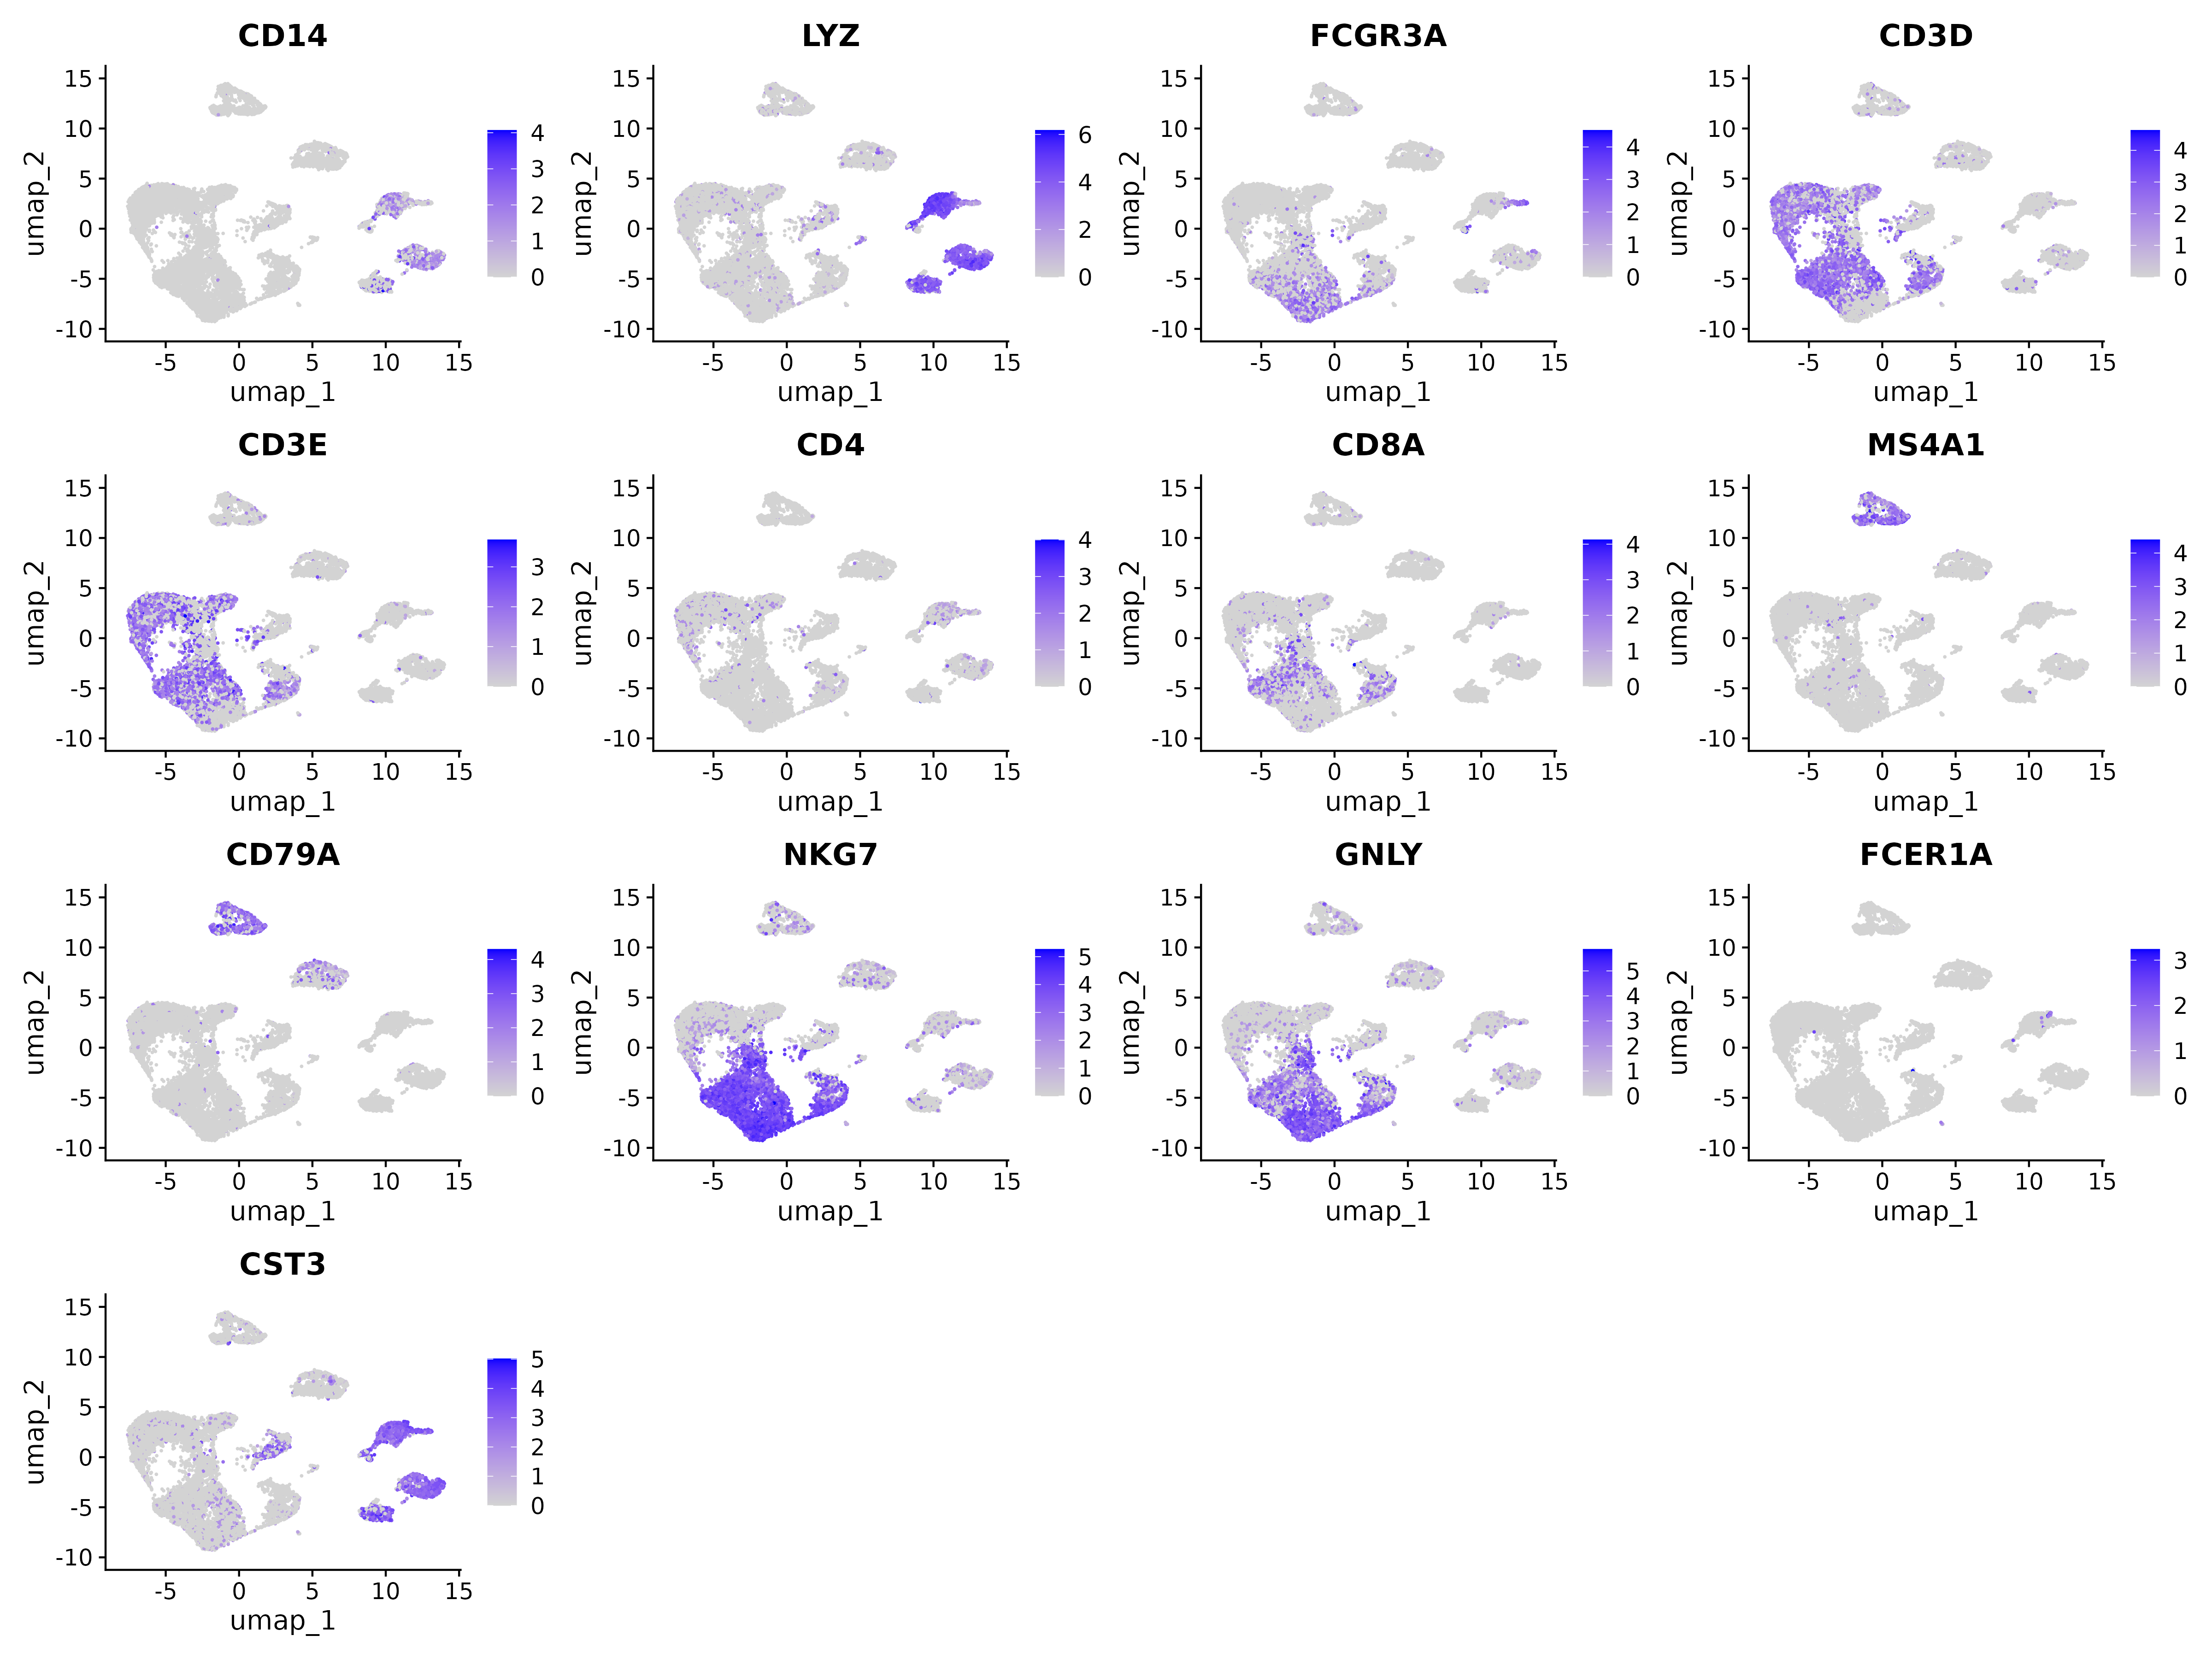
\includegraphics[width=\textwidth]{plots/phase5/phase5_marker_featureplots.png}
\end{center}

All 13 canonical markers from Phase 3 are applied to the GSE150861 UMAP:

\begin{itemize}[nosep]
  \item \textbf{CD14, LYZ, CST3}: all light up the same right-side clusters
        (6 and 10 in particular). The monocyte identity of the right mass is
        confirmed. FCGR3A (CD16) marks a smaller sub-cluster within that region,
        consistent with non-classical monocytes.
  \item \textbf{CD3D, CD3E, CD4, CD8A}: all concentrated in the large left
        continent, with CD4 and CD8A separating upper vs.\ lower sub-regions
        just as in Phase 3.
  \item \textbf{MS4A1, CD79A}: light up the two isolated top blobs
        exclusively — B cells.
  \item \textbf{NKG7, GNLY}: broad expression in the lower-left, marking
        NK cells / cytotoxic T cells.
  \item \textbf{FCER1A}: a small central cluster, consistent with
        dendritic cells.
\end{itemize}

The same spatial logic as Phase 3 is reproduced entirely independently.
This confirms that the cell-type architecture of PBMC datasets is stable
across different patients and sequencing runs.

\subsubsection*{Step 7b — SingleR annotation UMAP}

\begin{center}
  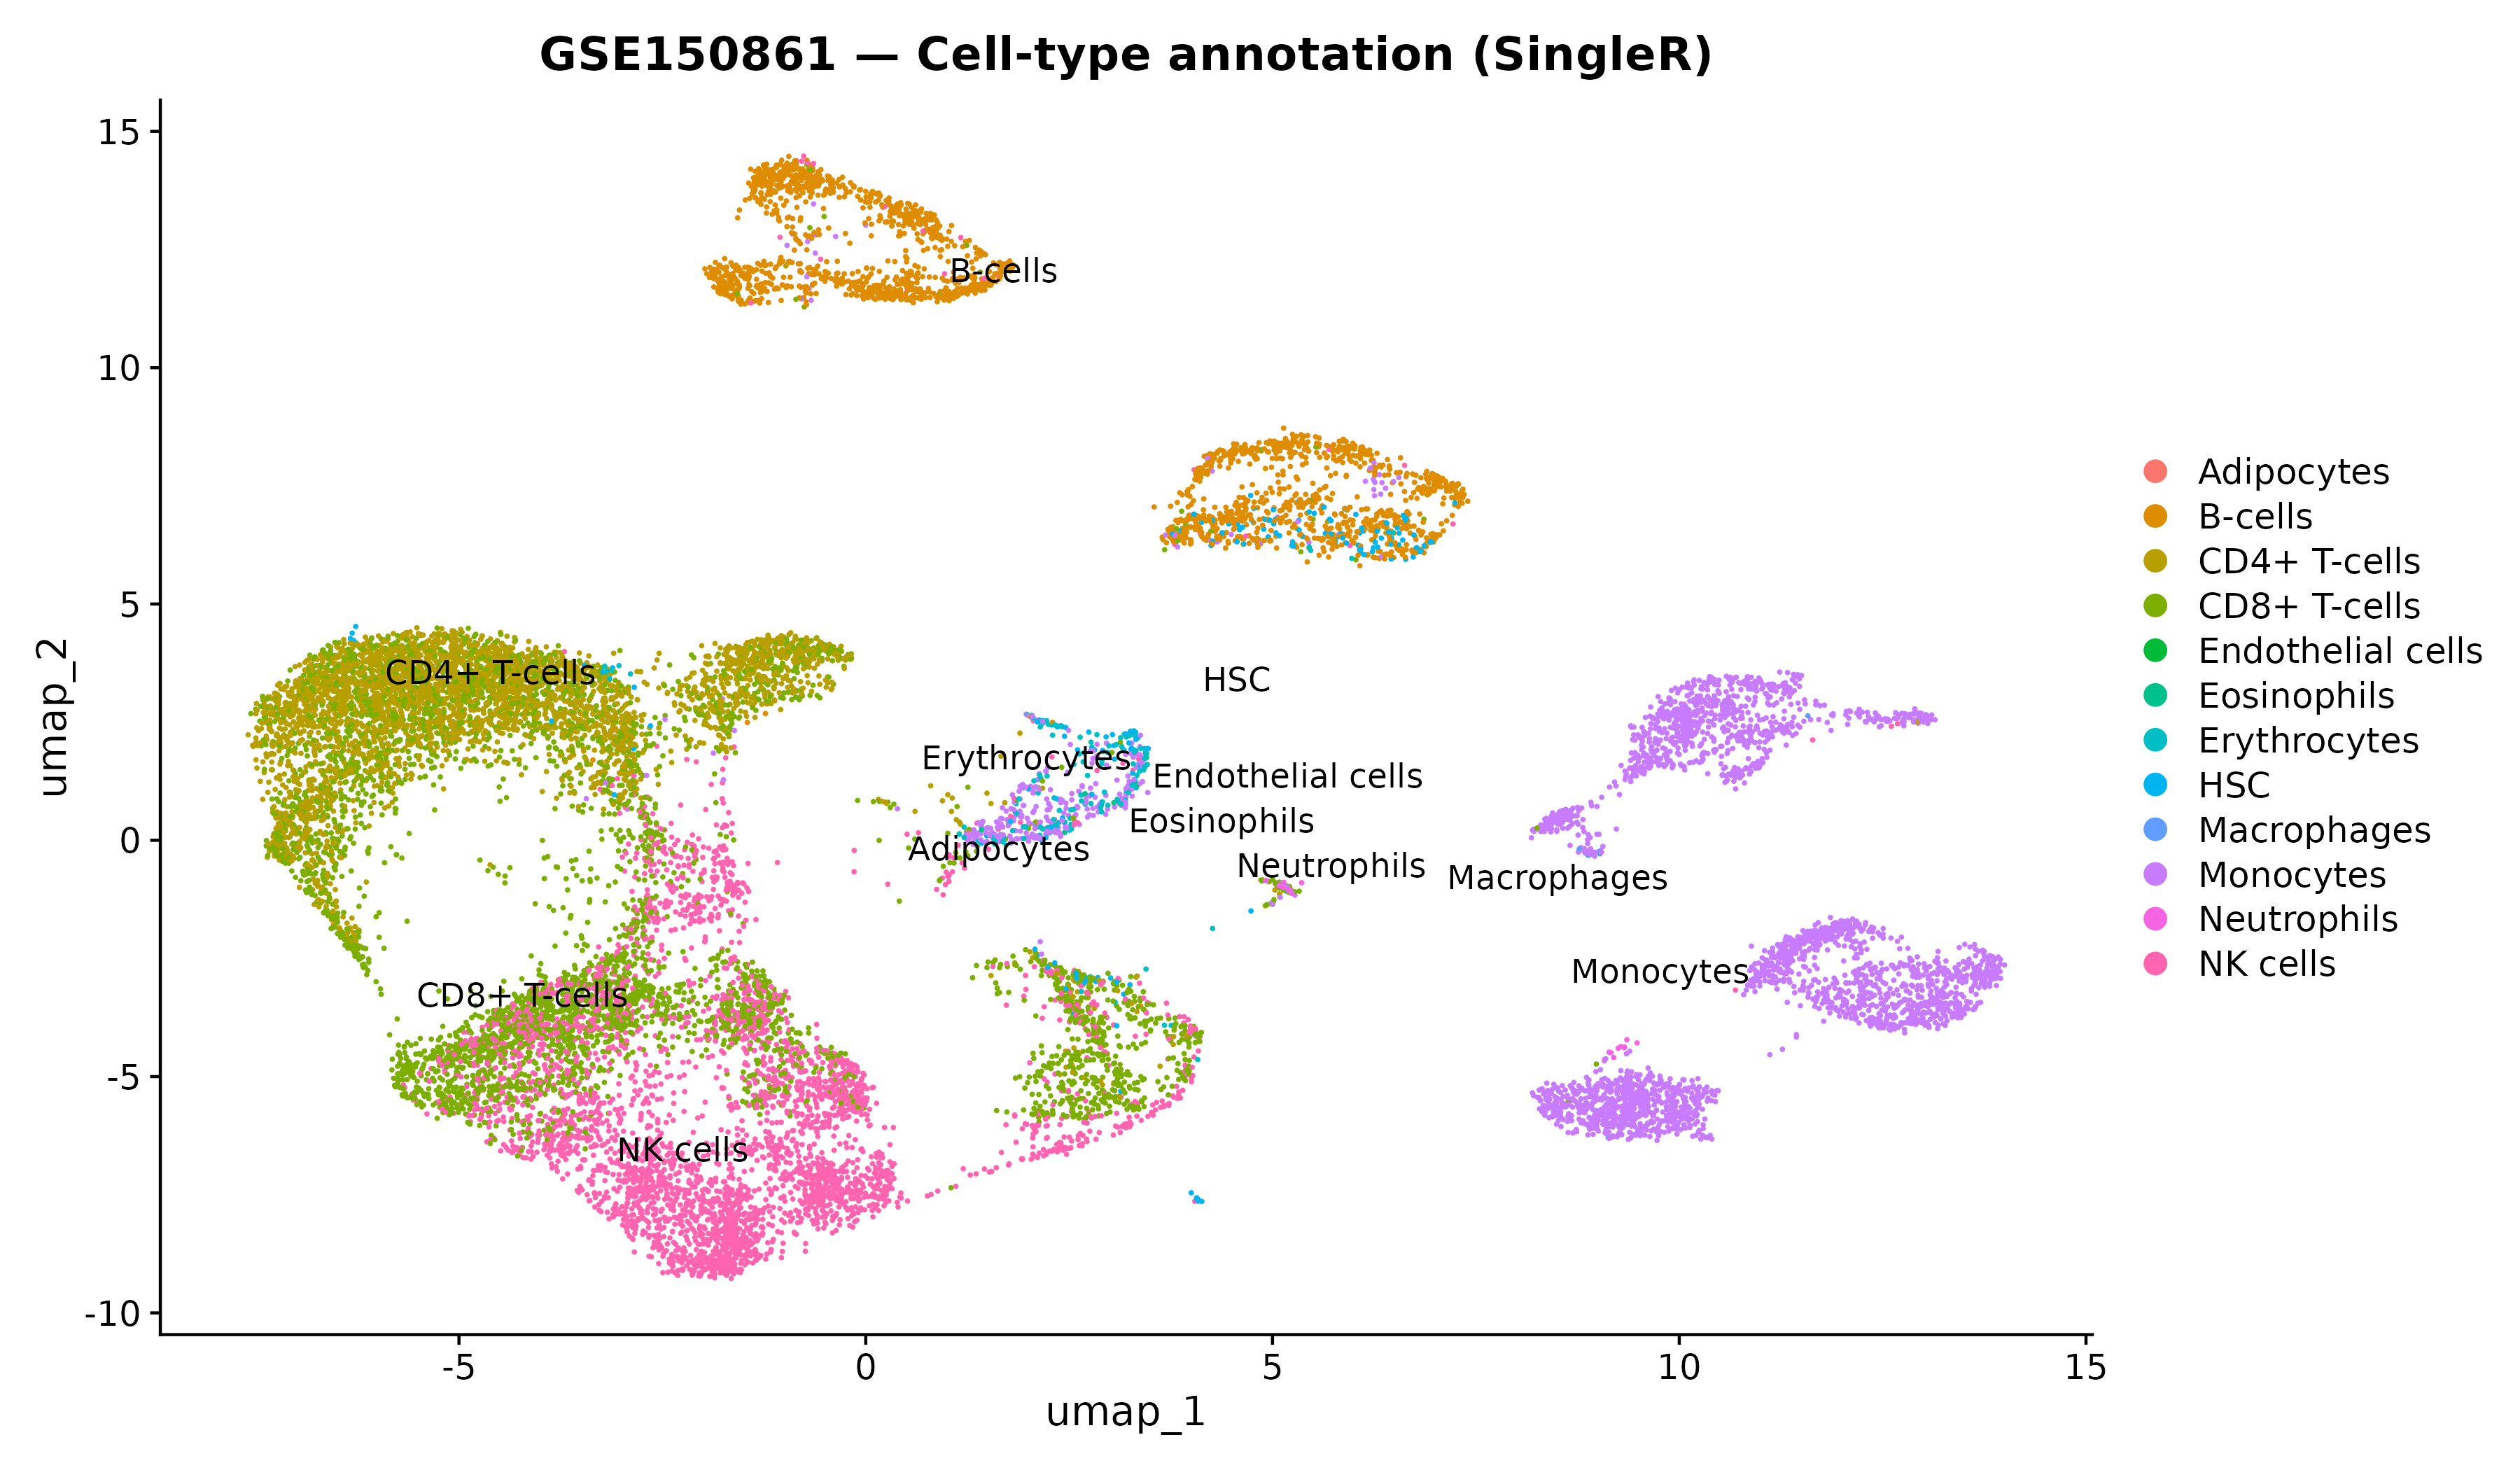
\includegraphics[width=0.95\textwidth]{plots/phase5/phase5_umap_celltype.png}
\end{center}

The SingleR annotation agrees with the manual markers on every major population:

\begin{itemize}[nosep]
  \item \textbf{Monocytes (purple):} the entire right-side mass (two blobs,
        consistent with classical and non-classical monocyte sub-sets).
  \item \textbf{CD4$^+$ T-cells (olive):} upper-left continent.
  \item \textbf{CD8$^+$ T-cells (green):} lower-left continent.
  \item \textbf{NK cells (hot pink):} lower-left, slightly below and
        intermixed with CD8$^+$ T cells — the same CD8/NK ambiguity
        seen in Phase 3.
  \item \textbf{B-cells (orange):} the two isolated top blobs, labeled
        cleanly with no cross-contamination from other types.
  \item \textbf{Rare populations (Erythrocytes, HSC, Eosinophils, Macrophages):}
        small scattered clusters in the central transition zone.
\end{itemize}

\subsection{Cell-type composition over time \small\normalfont\textit{(Step 11)}}

\begin{center}
  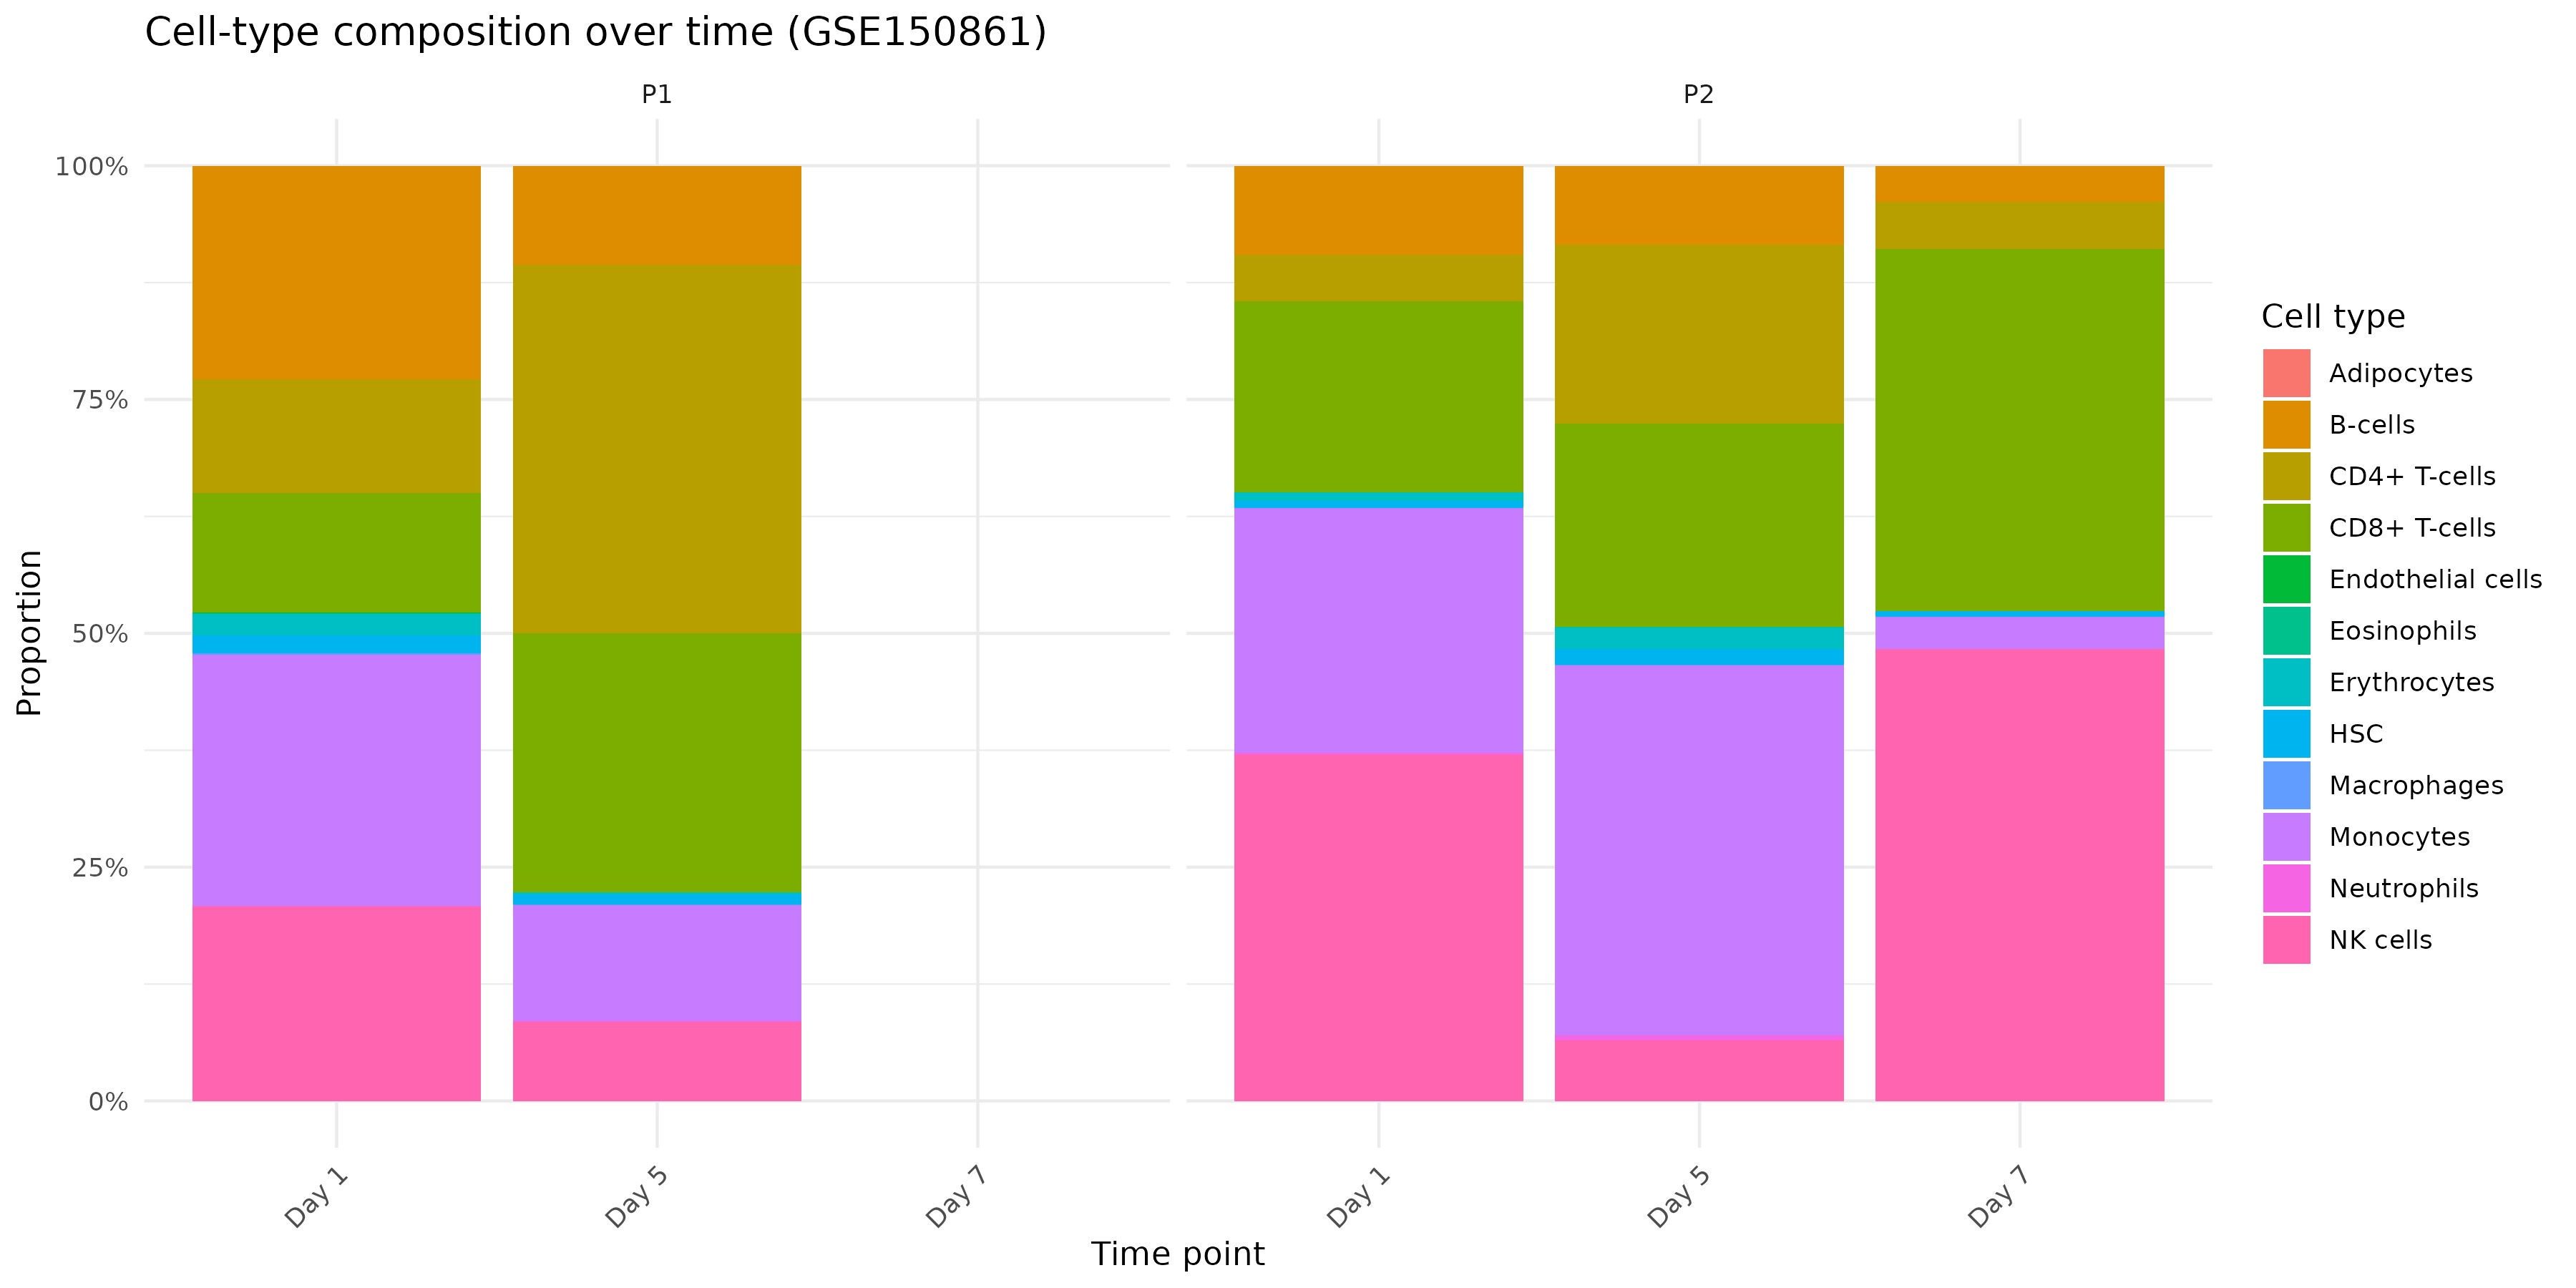
\includegraphics[width=\textwidth]{plots/phase5/phase5_composition_time.png}
\end{center}

The barplot shows the fraction of each cell type at each time point, split
by patient. This is the Phase 4 ``composition barplot'' idea applied
longitudinally.

\begin{itemize}[nosep]
  \item \textbf{P1 — Day 1:} Monocytes (purple) $\approx$30\% of cells.
        NK cells $\approx$20\%. CD4$^+$/CD8$^+$ T cells together $\approx$30\%.
  \item \textbf{P1 — Day 5:} Monocytes \textbf{collapse to $\approx$8\%}.
        CD8$^+$ T cells (bright green) dominate, rising to $\approx$50\%.
        NK cells also present. The monocyte compartment is dramatically reduced.
  \item \textbf{P1 — Day 7:} no data for P1 at Day 7 (shown as empty panel),
        suggesting this time point was not collected or passed QC for P1.
  \item \textbf{P2 — Day 1:} Monocytes $\approx$35\%. NK cells $\approx$35\%.
        T cells smaller.
  \item \textbf{P2 — Day 5:} Monocytes nearly disappear ($<$5\%). NK cells
        also drop sharply. CD4$^+$ and CD8$^+$ T cells together dominate.
  \item \textbf{P2 — Day 7:} NK cells \textbf{rebound dramatically to
        $\approx$50\%} — the largest single compartment at this time point.
        CD4$^+$ T cells also return. Monocytes remain low.
\end{itemize}

\textbf{Key message:} Tocilizumab treatment coincides with a rapid
collapse of the monocyte compartment and a rebound of lymphocytes.
This mirrors the Phase 4 observation that monocyte expansion is a
feature of active disease — and it reverses under treatment.

\subsection{Co-activation replication scatter \small\normalfont\textit{(Step 10)}}

\begin{center}
  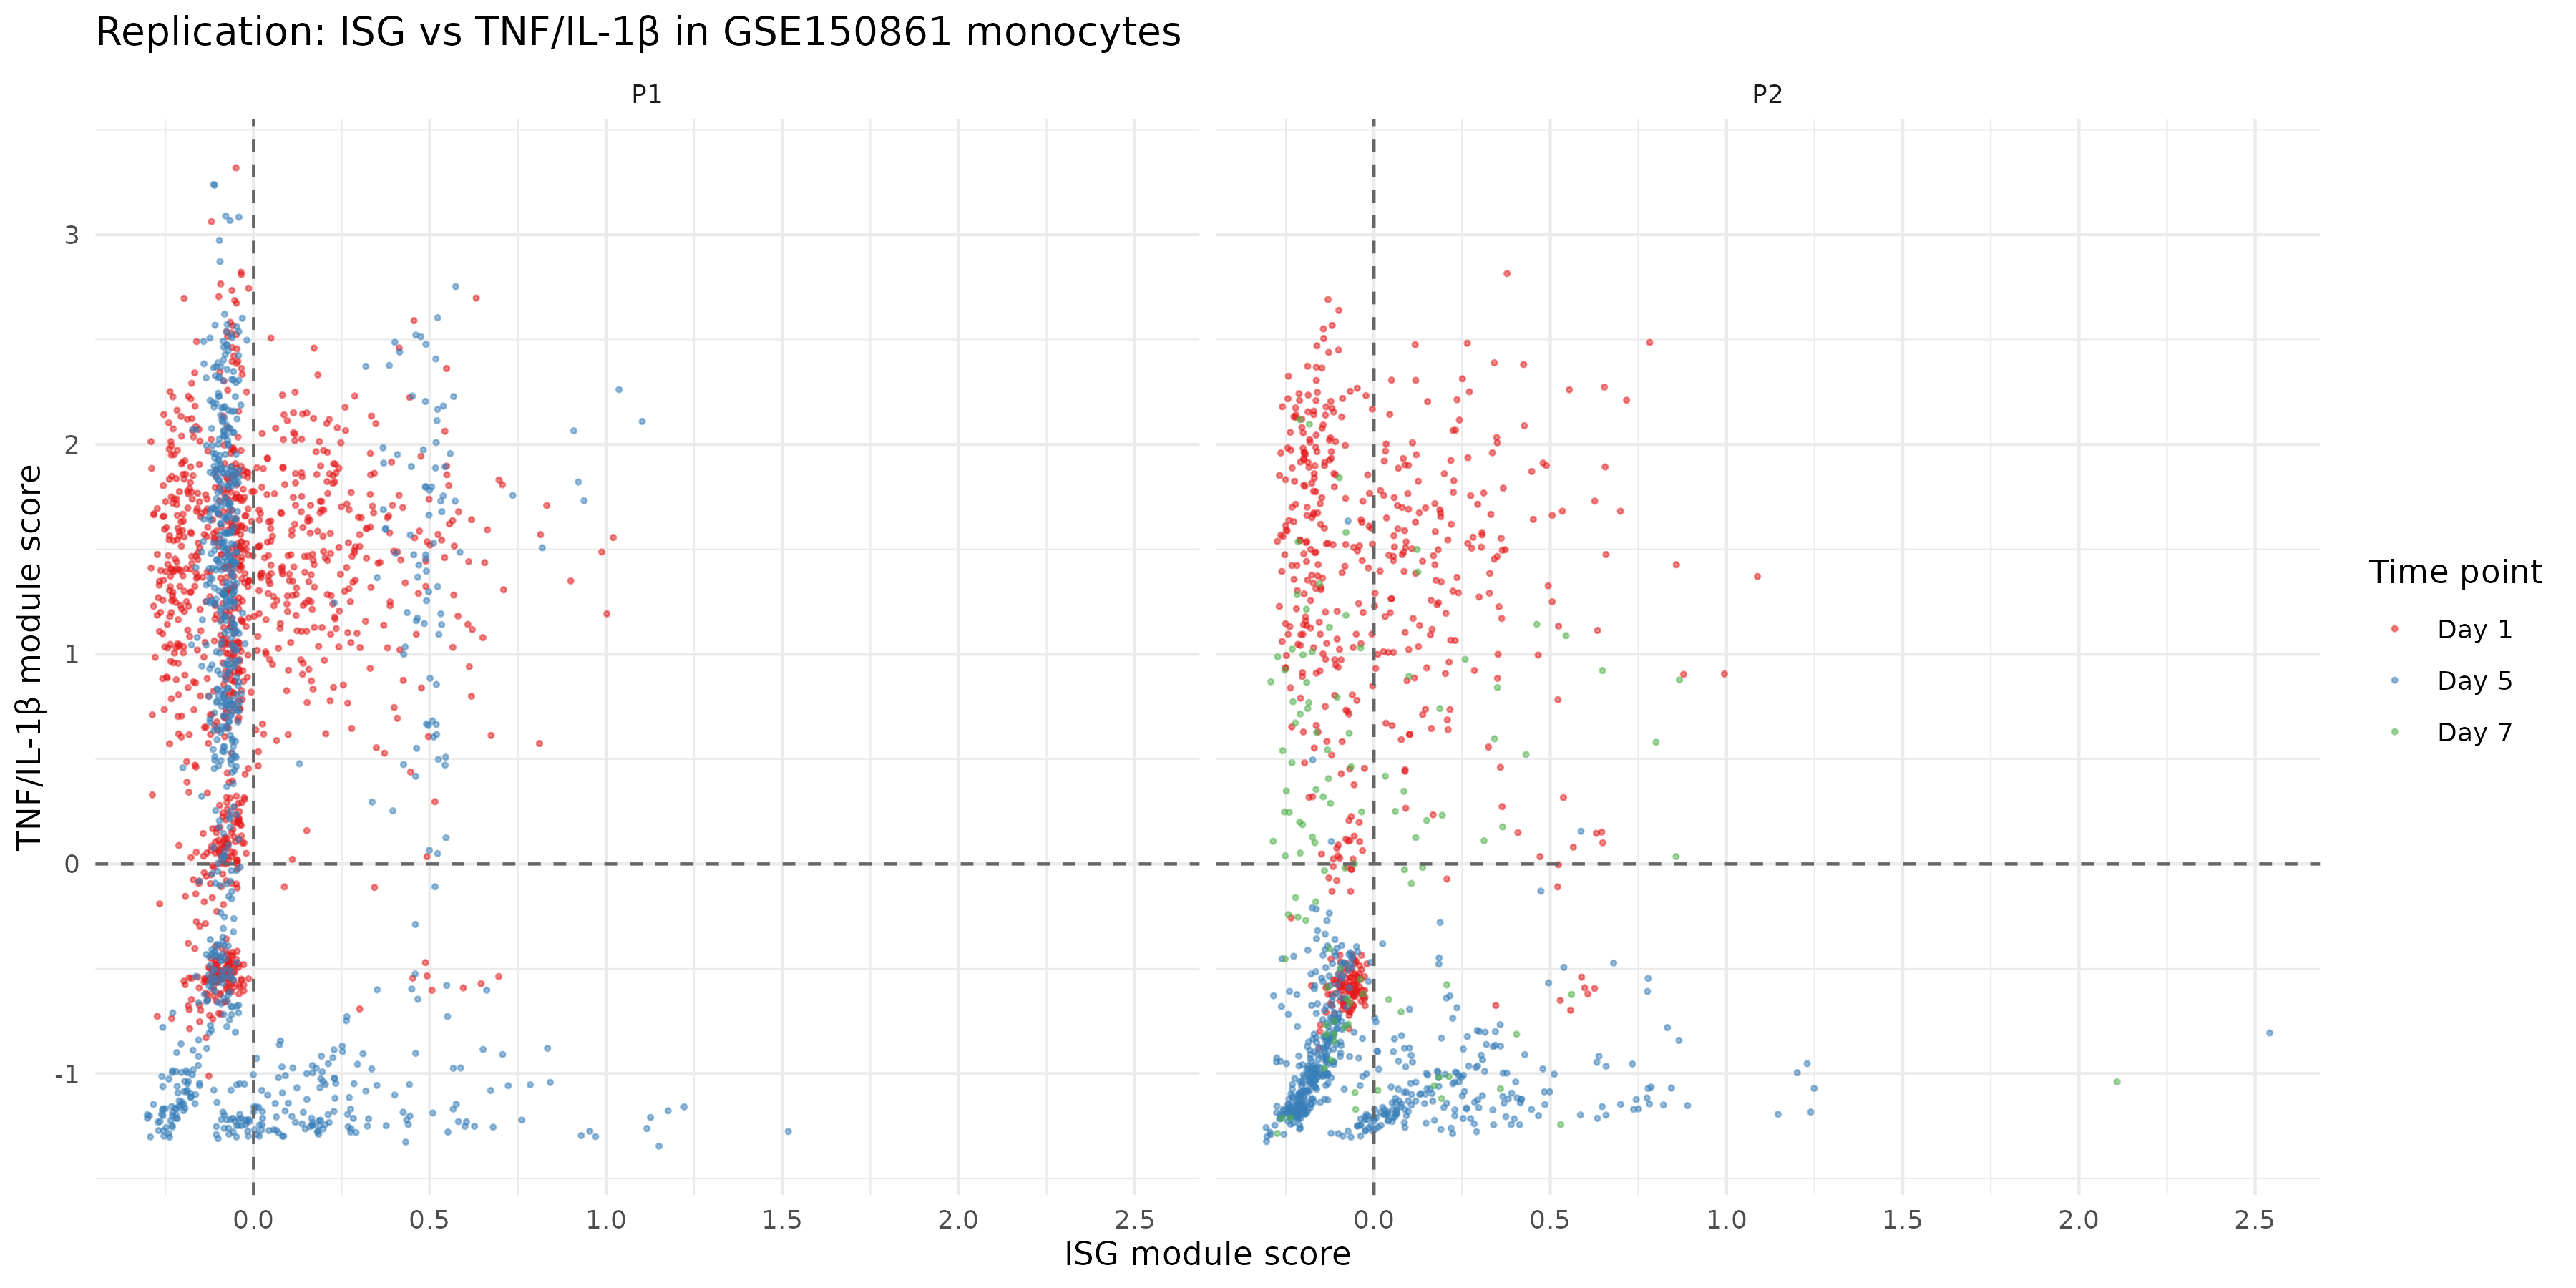
\includegraphics[width=\textwidth]{plots/phase5/phase5_coactivation_scatter.png}
\end{center}

This is the central replication plot: the same ISG vs TNF/IL-1$\beta$
scatter from Phase 4, now in GSE150861, faceted by patient and coloured
by time point.

\begin{itemize}[nosep]
  \item \textbf{Day 1 (red dots):} in both P1 and P2, Day 1 cells
        are concentrated in the \textbf{top-left} quadrant (high TNF/IL-1$\beta$,
        low ISG) and the \textbf{top-right} quadrant (co-activated).
        The co-activated top-right population is clearly present on Day 1
        \textbf{in both patients}. This directly replicates the Phase 4 finding.

  \item \textbf{Day 5 (blue dots):} cells shift downward. The top quadrants
        are less populated. TNF/IL-1$\beta$ scores drop substantially.
        Fewer cells are in the co-activated quadrant. This is the first
        quantitative sign that Tocilizumab is suppressing the inflammatory
        program.

  \item \textbf{Day 7 (green dots):} the smallest number of cells (fewest
        monocytes remaining). They appear scattered and mostly in the lower
        half — the inflammatory component is further reduced in P1 and shows
        partial recovery in P2.

  \item \textbf{Asymmetry between P1 and P2:} P2 monocytes are more tightly
        clustered near $x = -0.3$ (ISG near zero) with high TNF/IL-1$\beta$
        on Day 1. P1 monocytes are spread more widely in ISG score.
        This patient-to-patient variability is consistent with Phase 4,
        where donor heterogeneity was high even within the same severity group.
\end{itemize}

\subsection{Longitudinal dynamics and Tocilizumab effect \small\normalfont\textit{(Steps 11–12)}}

\subsubsection*{Step 11 — Longitudinal line plots}

\begin{center}
  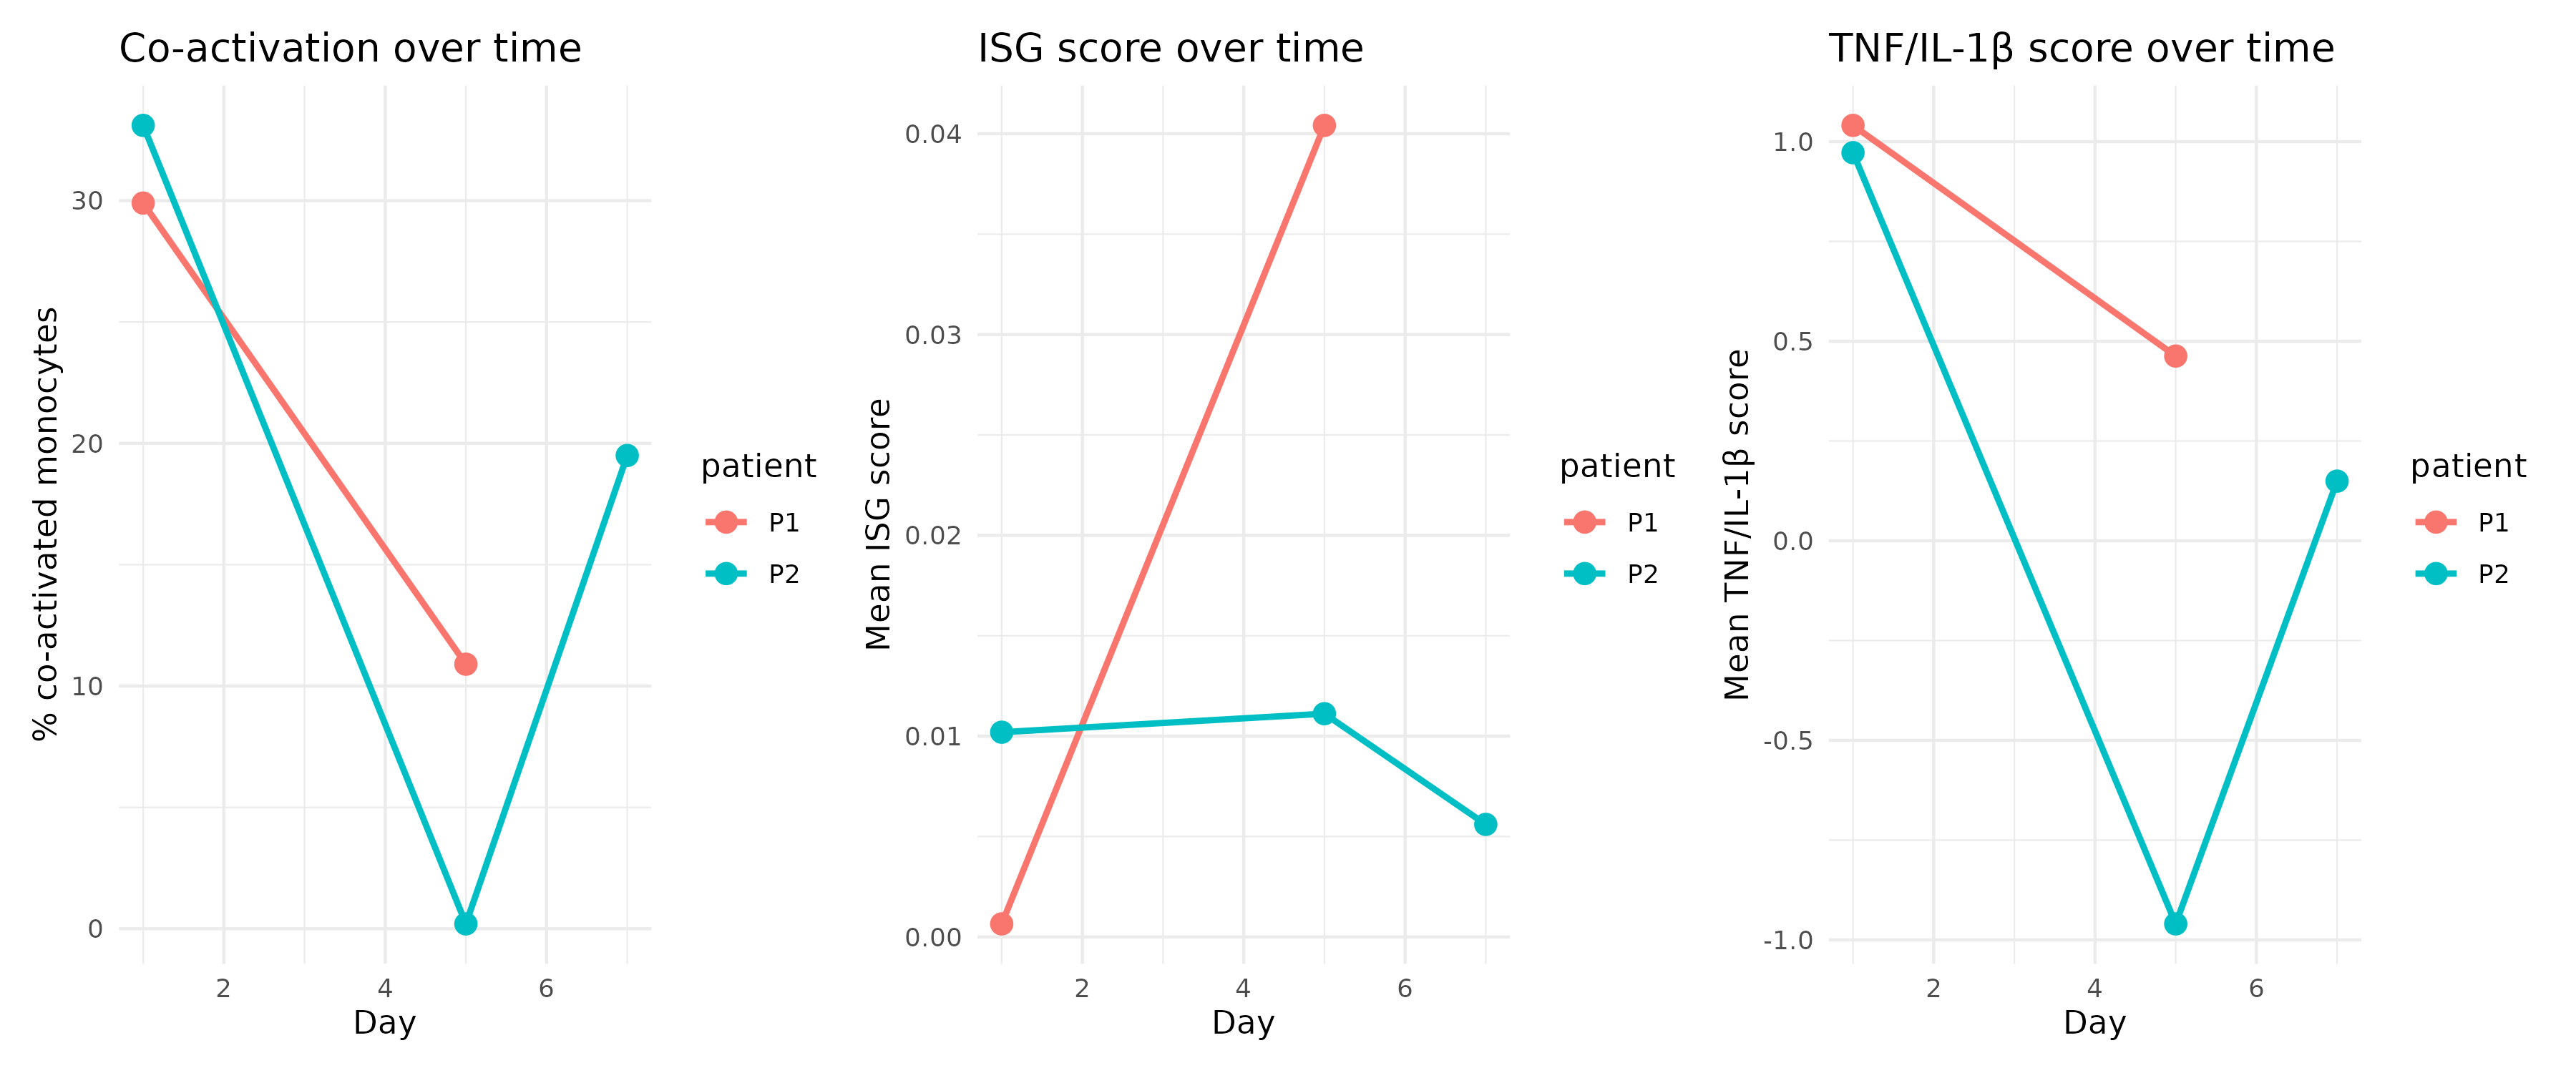
\includegraphics[width=\textwidth]{plots/phase5/phase5_longitudinal_dynamics.png}
\end{center}

Each point is one patient at one time point. Lines connect the same patient
across days.

\textit{Left — Co-activation \% over time:}
\begin{itemize}[nosep]
  \item Both patients start with \textbf{$\sim$30--35\% co-activated monocytes}
        on Day 1 — matching the high outlier donors seen in Phase 4.
  \item By Day 5, both drop sharply: P1 to $\sim$11\%, P2 to $\approx$0\%.
  \item By Day 7: P1 is missing; P2 partially recovers to $\sim$20\%.
  \item The consistent Day 1 $\to$ Day 5 drop across both patients, \textit{in
        the same direction}, is the key result. With only two patients it
        cannot be tested statistically, but the direction is unambiguous.
\end{itemize}

\textit{Middle — ISG score over time:}
\begin{itemize}[nosep]
  \item P2 starts near zero and stays low across all days —
        no strong antiviral response at the ISG level.
  \item P1 starts near zero on Day 1, then \textbf{rises to 0.04 on Day 5}.
        This is the opposite direction from the TNF/IL-1$\beta$ response.
        The ISG program either persists or increases while the inflammatory
        program is suppressed by Tocilizumab.
  \item This is biologically coherent: Tocilizumab blocks IL-6-mediated
        signaling, which suppresses the inflammasome-driven inflammatory
        genes (TNF, IL1B) but does not inhibit the interferon pathway
        (which is driven by type-I interferons, not IL-6).
\end{itemize}

\textit{Right — TNF/IL-1$\beta$ score over time:}
\begin{itemize}[nosep]
  \item Both patients start \textbf{high ($\approx +1.0$)} on Day 1.
  \item Both \textbf{drop sharply} by Day 5: P1 to $\approx +0.5$,
        P2 to $\approx -1.0$ (near-complete suppression).
  \item P2 partially rebounds to $\approx +0.2$ by Day 7, while P1's Day 7
        data is absent.
  \item The Day 1 $\to$ Day 5 drop in both patients is the clearest
        Tocilizumab signal: blocking IL-6R measurably reduces the
        TNF/IL-1$\beta$ program in monocytes within 4 days.
\end{itemize}

\subsubsection*{Step 12 — Violin plots by time point}

\begin{center}
  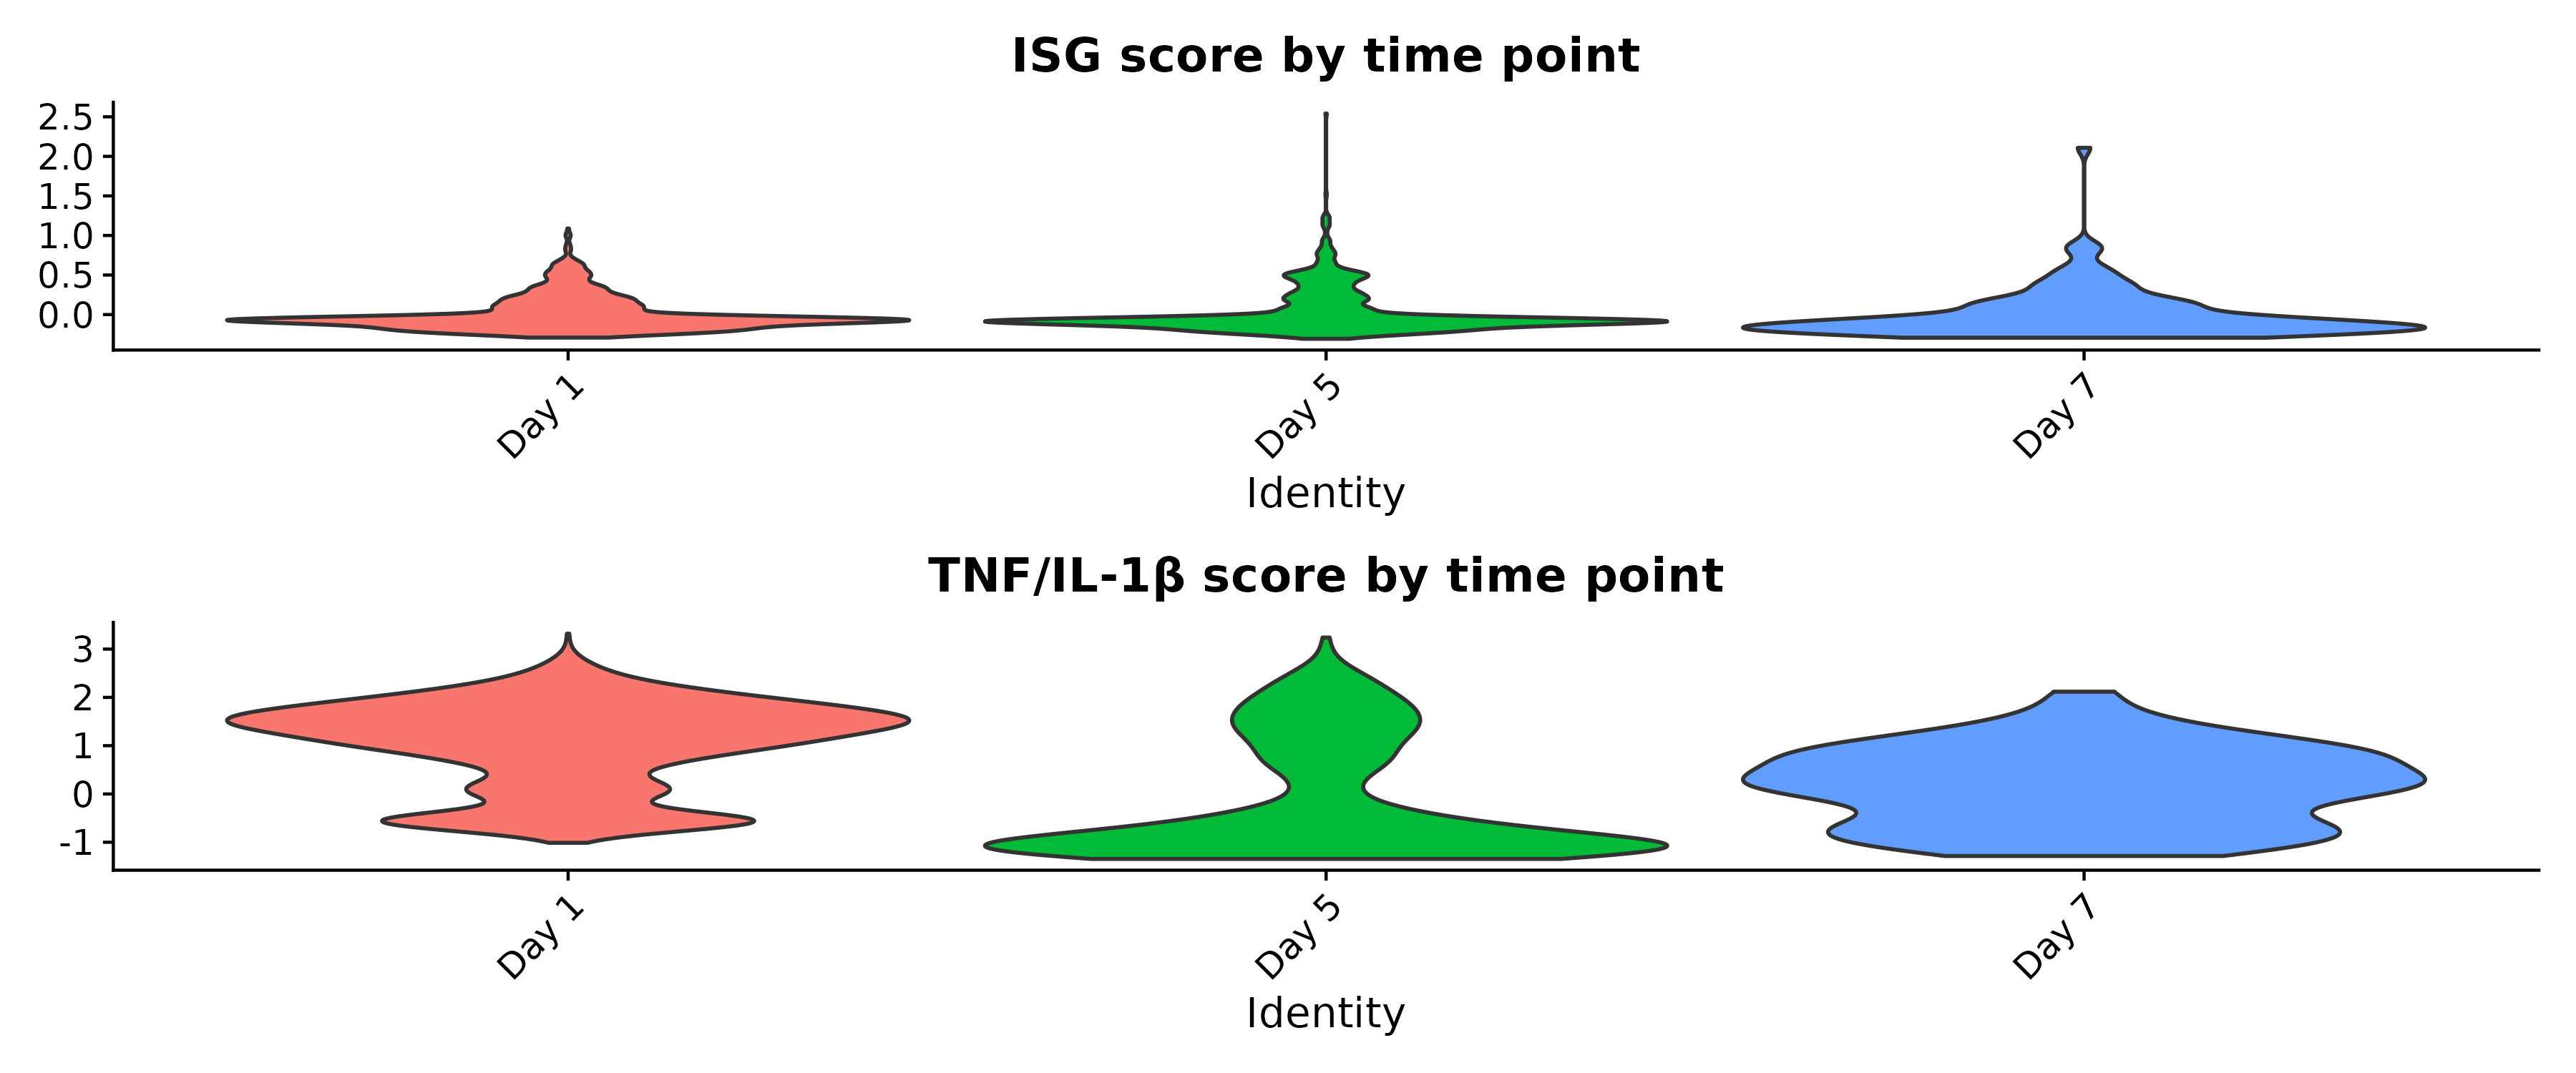
\includegraphics[width=\textwidth]{plots/phase5/phase5_toci_violin.png}
\end{center}

The violin plots show the full distribution of all monocytes at each time point.

\textit{Top panel — ISG score:}
\begin{itemize}[nosep]
  \item Day 1: narrow violin centered near 0, extending slightly above.
  \item Day 5: \textbf{the body widens and the upper spike grows} —
        consistent with the P1-driven ISG rise seen in the line plot.
        There are more ISG-high cells on Day 5 than on Day 1.
  \item Day 7: the ISG body is still present but slightly narrower.
\end{itemize}

\textit{Bottom panel — TNF/IL-1$\beta$ score:}
\begin{itemize}[nosep]
  \item \textbf{Day 1}: very wide, heavy-bodied violin spanning from $-1$
        to $+3$. The entire upper range is populated — many cells with
        very high inflammatory scores. This is the active disease state.
  \item \textbf{Day 5}: the violin \textbf{collapses dramatically}.
        It becomes narrow and bimodal, with most cells near 0 or below.
        The upper inflammatory tail is largely gone. This is the clearest
        visual demonstration of Tocilizumab suppressing the program.
  \item \textbf{Day 7}: broader than Day 5 but in a new shape — a wide
        flat body rather than the tall spiky Day 1 shape. Partial recovery
        of the inflammatory program is visible.
\end{itemize}

\subsection{Phase 5 conclusion}

Phase 5 achieves its goal: the co-activated monocyte state from Phase 4
\textbf{replicates in an independent dataset}. The key findings are:

\begin{enumerate}[nosep]
  \item \textbf{Replication confirmed.}
        Both patients in GSE150861 have $\sim$30\% co-activated monocytes
        on Day 1 — matching the range seen in Phase 4 severe donors and
        validating that the Phase 4 signal was not dataset-specific.

  \item \textbf{The cell-type structure is stable across datasets.}
        The UMAP topology, SingleR labels, and marker gene patterns are
        essentially identical to Phase 3, despite entirely different
        patients and a different study design.

  \item \textbf{The co-activated state is responsive to treatment.}
        Tocilizumab reduces co-activation from $\sim$30\% to near zero
        within 4 days in both patients, primarily by suppressing the
        TNF/IL-1$\beta$ component. The ISG (antiviral) component is
        unaffected or slightly increases — exactly what is expected
        given that Tocilizumab targets the IL-6 axis, not the interferon
        axis.

  \item \textbf{The monocyte compartment collapses under treatment.}
        As monocyte co-activation drops, monocytes also decline as
        a fraction of blood cells, replaced by a lymphocyte rebound.
        The blood composition shift mirrors the severity-related
        shift seen in Phase 4.

  \item \textbf{Limitation: only 2 patients.}
        With N = 2, no statistical test is meaningful.
        Both patients show consistent effects in the same direction,
        which is strong qualitative evidence, but it cannot substitute
        for a larger cohort.
\end{enumerate}

\textbf{Together, Phases 4 and 5 establish the single-cell part of
the story:} co-activated monocytes exist, are enriched in severe
COVID, replicate in an independent cohort, and are suppressed by
the treatment that reduces disease severity.
The next phase asks whether the same signal is detectable in bulk
RNA-seq data, where individual cells are not distinguished.

% ─────────────────────────────────────────────
\section{Phase 6 — scRNA-seq Visualization Summary}
% ─────────────────────────────────────────────

\subsection{Phase 6 overview — the big picture}

\textbf{Phases 3–5 produced the results. Phase 6 assembles them into a clean, complete visual story.}

At this point we have:
\begin{itemize}[nosep]
  \item An annotated UMAP with all PBMC cell types (Phase 3).
  \item Evidence that monocytes expand and gain an inflammatory program in severe COVID (Phase 4).
  \item Replication of the co-activated monocyte state in an independent dataset (Phase 5).
\end{itemize}

Phase 6 re-creates all the key plots in consistent, publication-quality style and assembles a
four-panel summary figure that tells the whole scRNA-seq story at a glance.
No new analysis is done — this phase is about \textit{presentation}.

\subsection{The annotated UMAP}

\begin{center}
  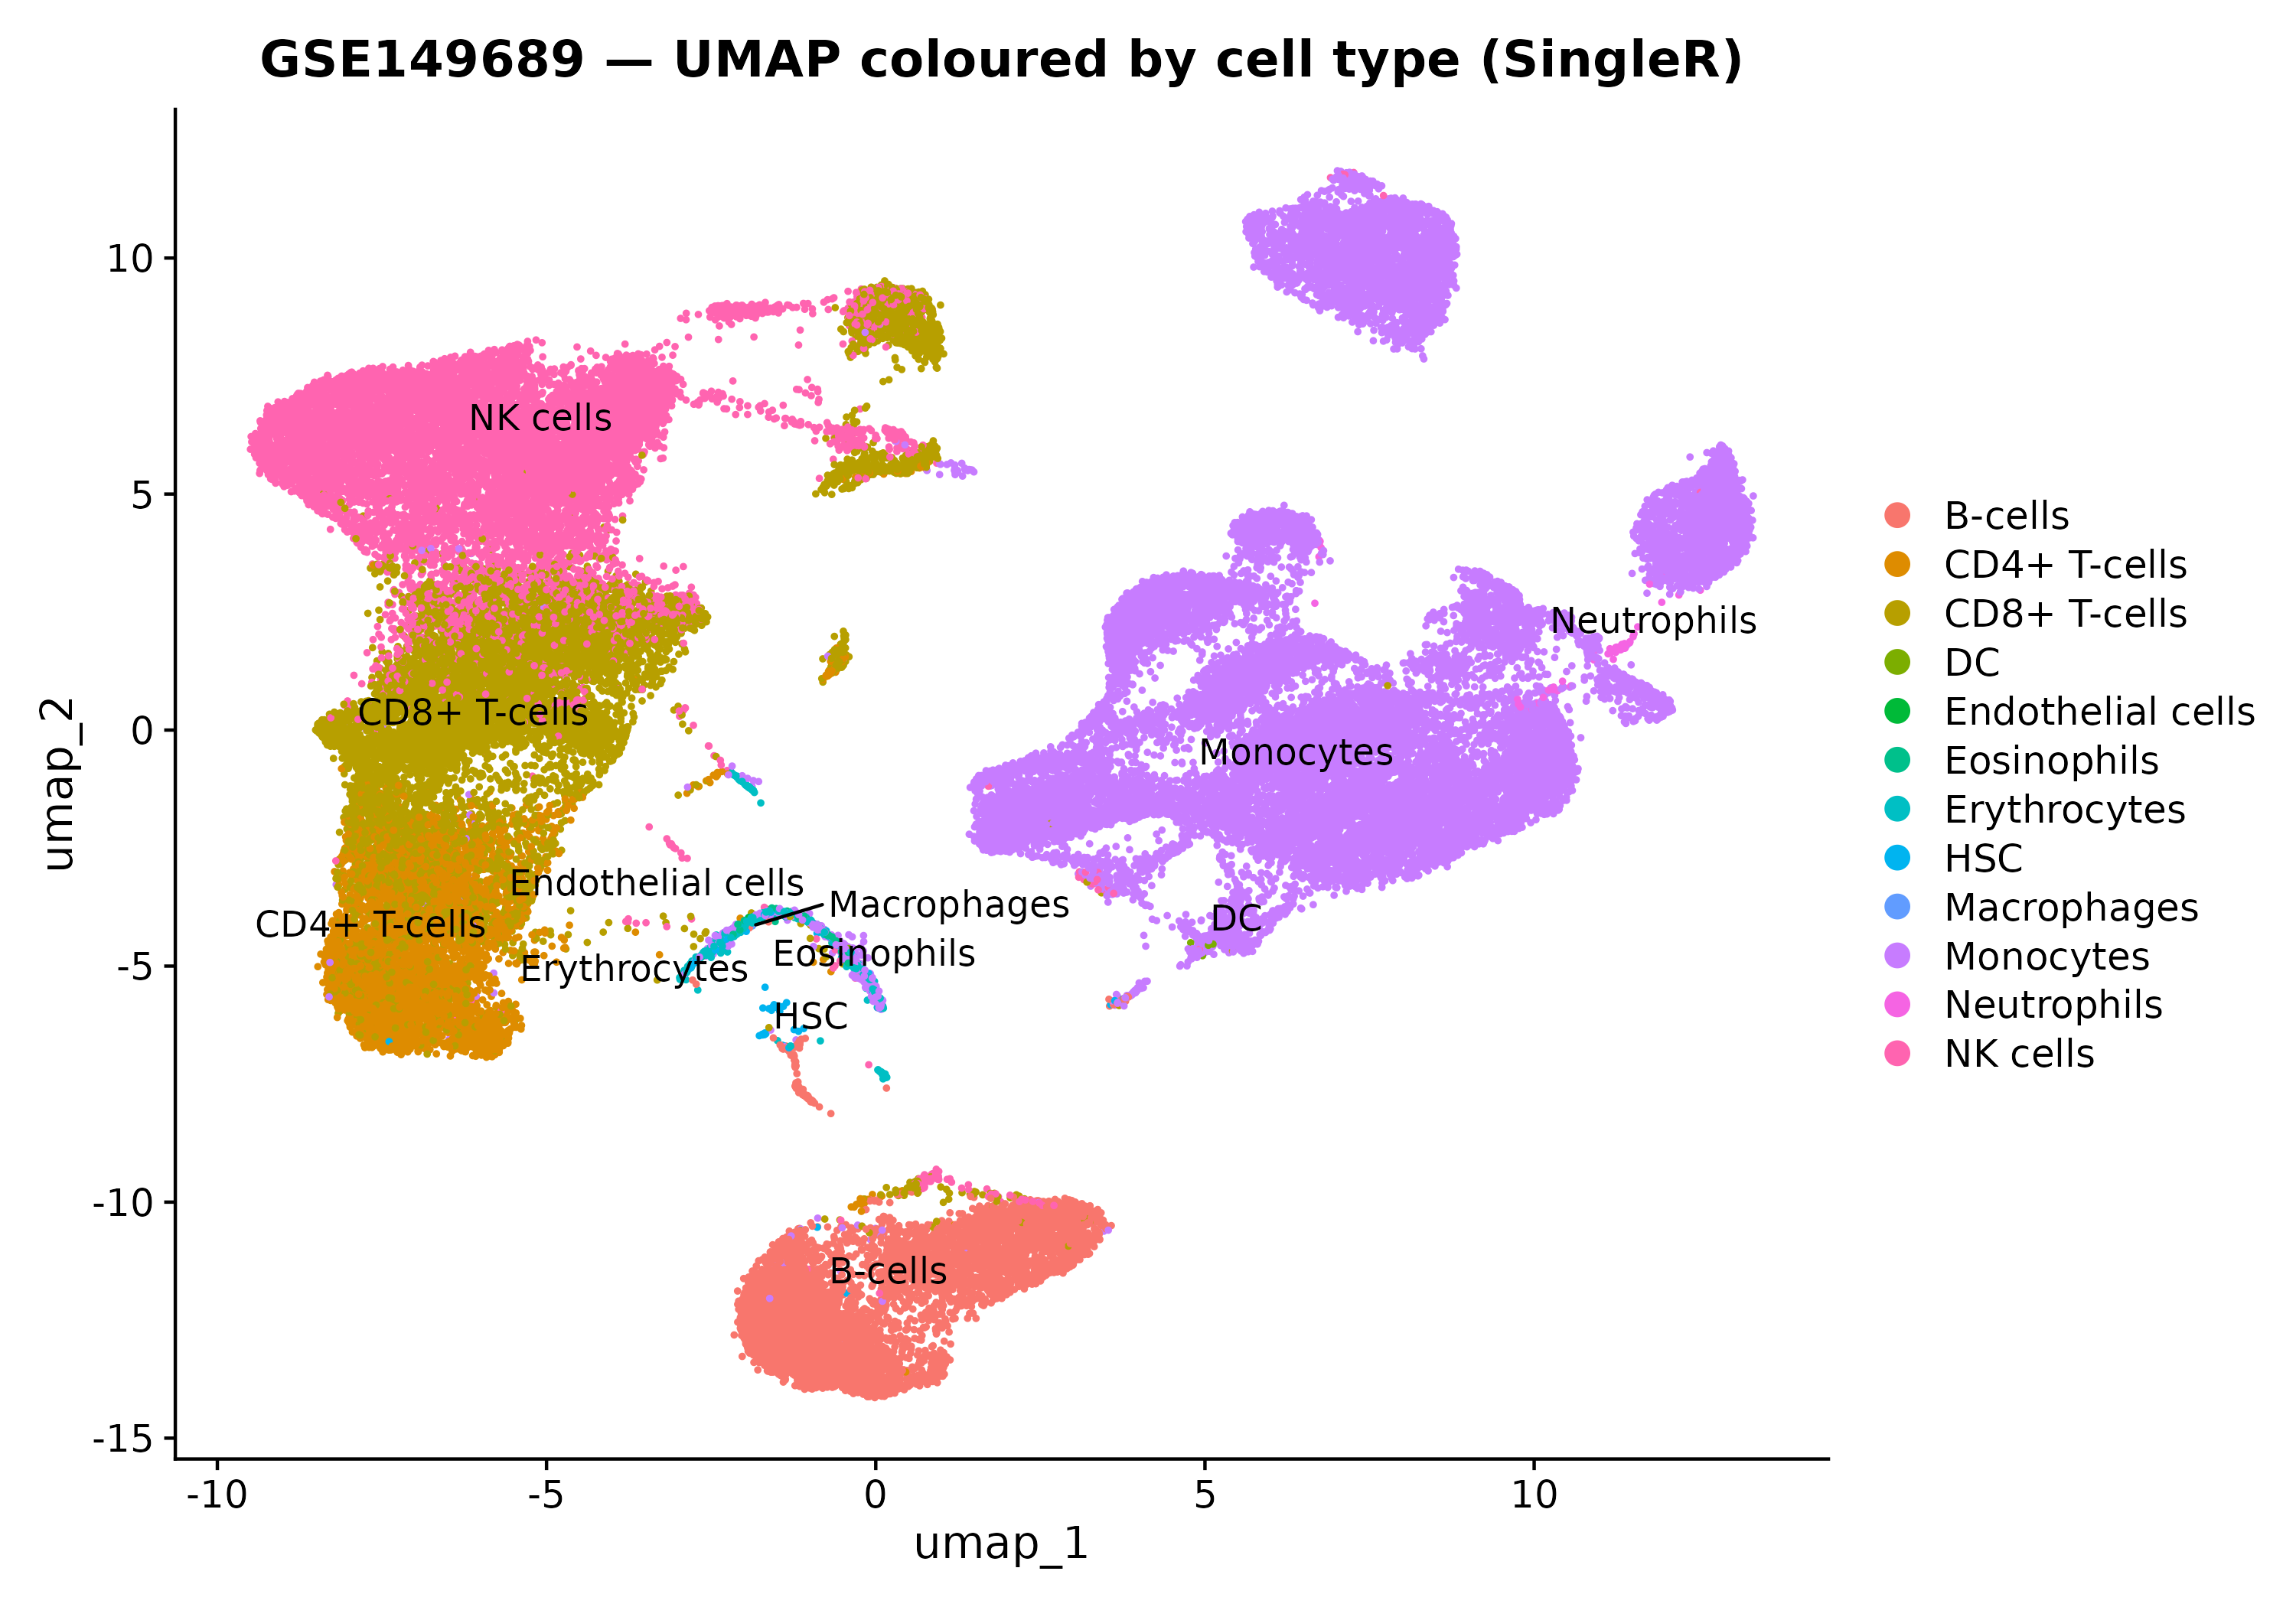
\includegraphics[width=0.9\textwidth]{plots/phase6/phase6_01_umap_celltype.png}
\end{center}

This is the final reference map: the full GSE149689 dataset (55,548 cells) coloured by
SingleR cell-type label, with text labels placed on the plot.

The five major compartments are clearly resolved:
\begin{itemize}[nosep]
  \item \textbf{Monocytes (purple)} — the large right-side mass, the dominant cell type
        in this COVID PBMC dataset.
  \item \textbf{NK cells (pink)} — upper-left, a distinct and well-separated island.
  \item \textbf{CD8$^+$ T-cells (olive)} — middle-left, next to NK cells.
  \item \textbf{CD4$^+$ T-cells (orange)} — lower-left pocket.
  \item \textbf{B-cells (salmon)} — bottom isolated island, completely separate from
        everything else.
\end{itemize}
Smaller populations are also labeled: DC (dendritic cells) sitting between myeloid and
lymphoid continents, Neutrophils in the upper-right monocyte area, and rare cells
(Erythrocytes, HSC, Eosinophils, Macrophages) scattered in the center transition zone.

This single plot is the map the reader needs to orient all further analysis.

\subsection{Cell-type composition by severity}

\subsubsection*{UMAP split by severity}

\begin{center}
  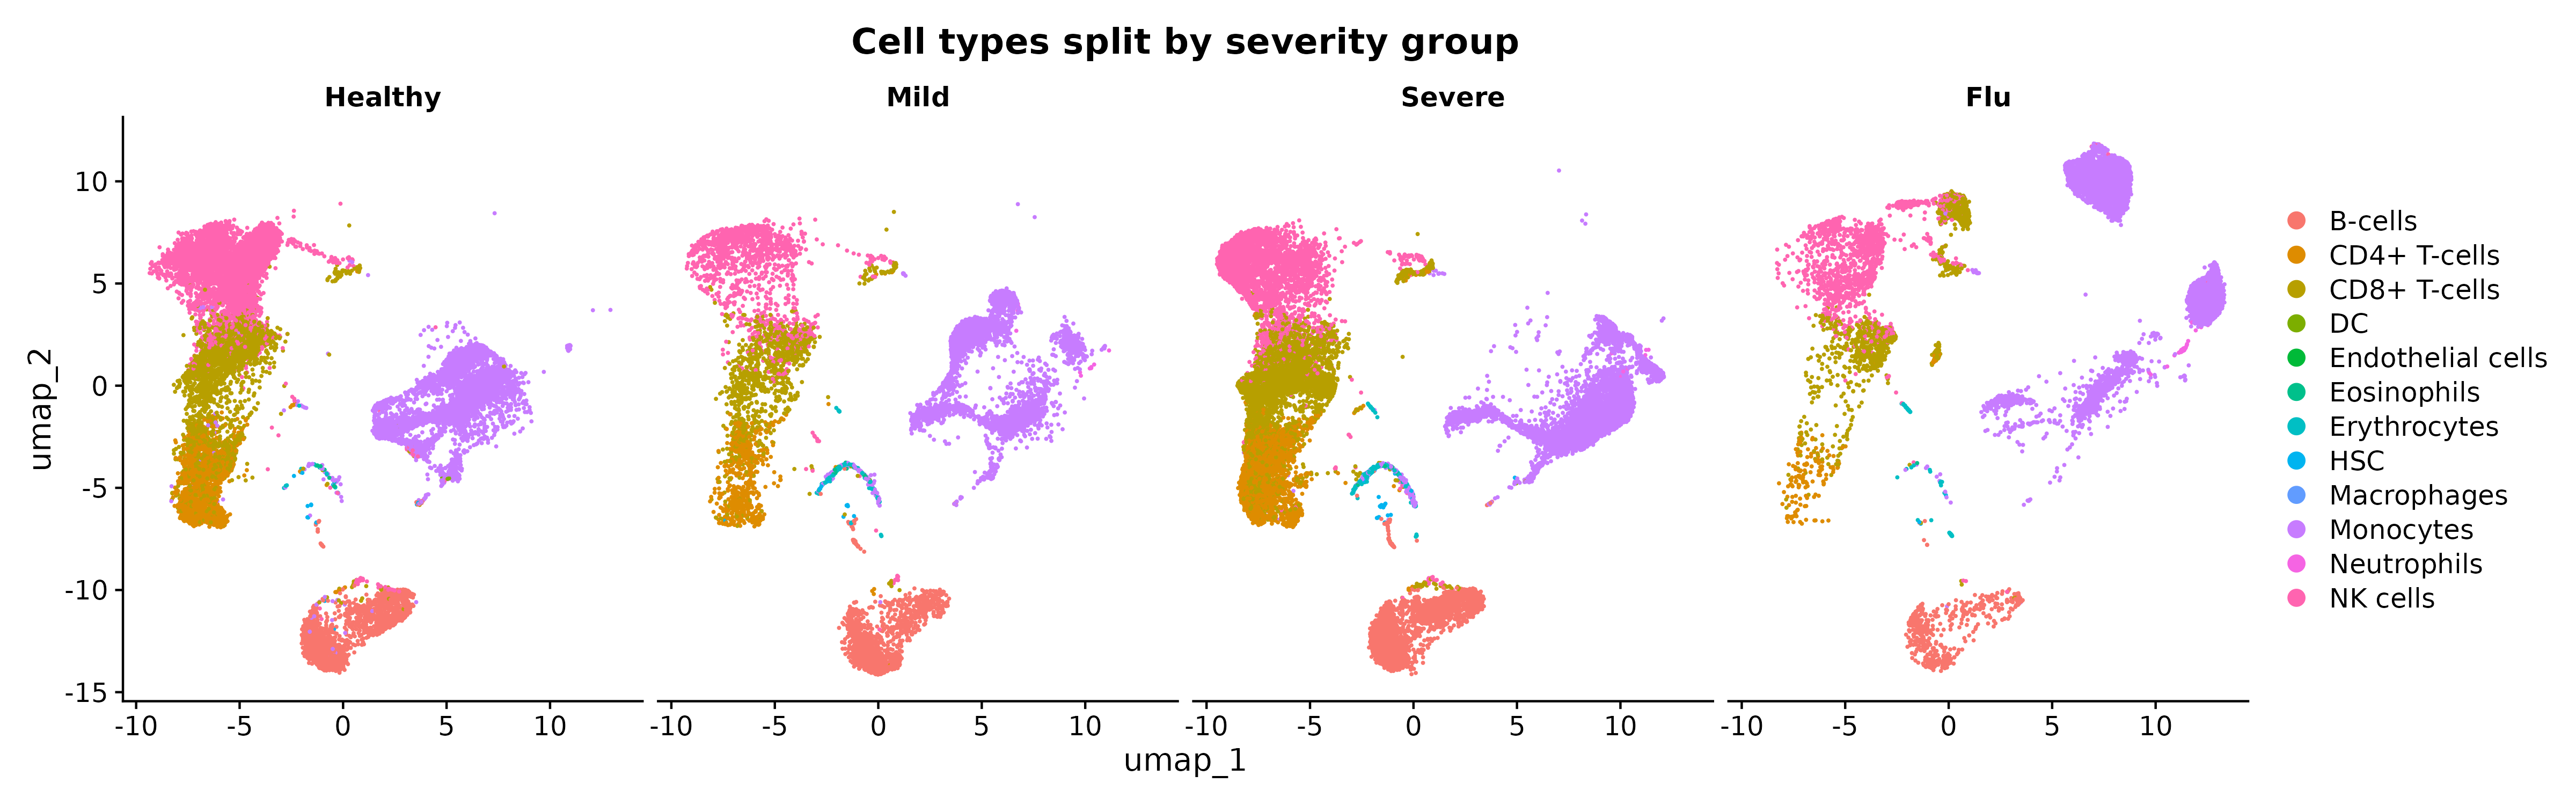
\includegraphics[width=\textwidth]{plots/phase6/phase6_02_umap_split_severity.png}
\end{center}

Each panel shows only cells from one condition, coloured by cell type.
The composition shifts are visible by eye:

\begin{itemize}[nosep]
  \item \textbf{Healthy:} the UMAP is balanced. The left lymphoid continent (T, NK cells)
        and the right monocyte mass are roughly comparable in density.
  \item \textbf{Mild:} similar to Healthy. No dramatic shift yet.
  \item \textbf{Severe:} the monocyte (purple) mass on the right is clearly bigger and
        denser. The left continent is visibly thinner — \textbf{T and NK cells are depleted}.
  \item \textbf{Flu:} the monocyte mass occupies most of the plot. Strikingly, a large
        separate purple blob drifts to the far top-right — a Flu-specific monocyte
        sub-state that is transcriptionally distinct enough to detach from the main mass.
\end{itemize}

\subsubsection*{Composition barplot}

\begin{center}
  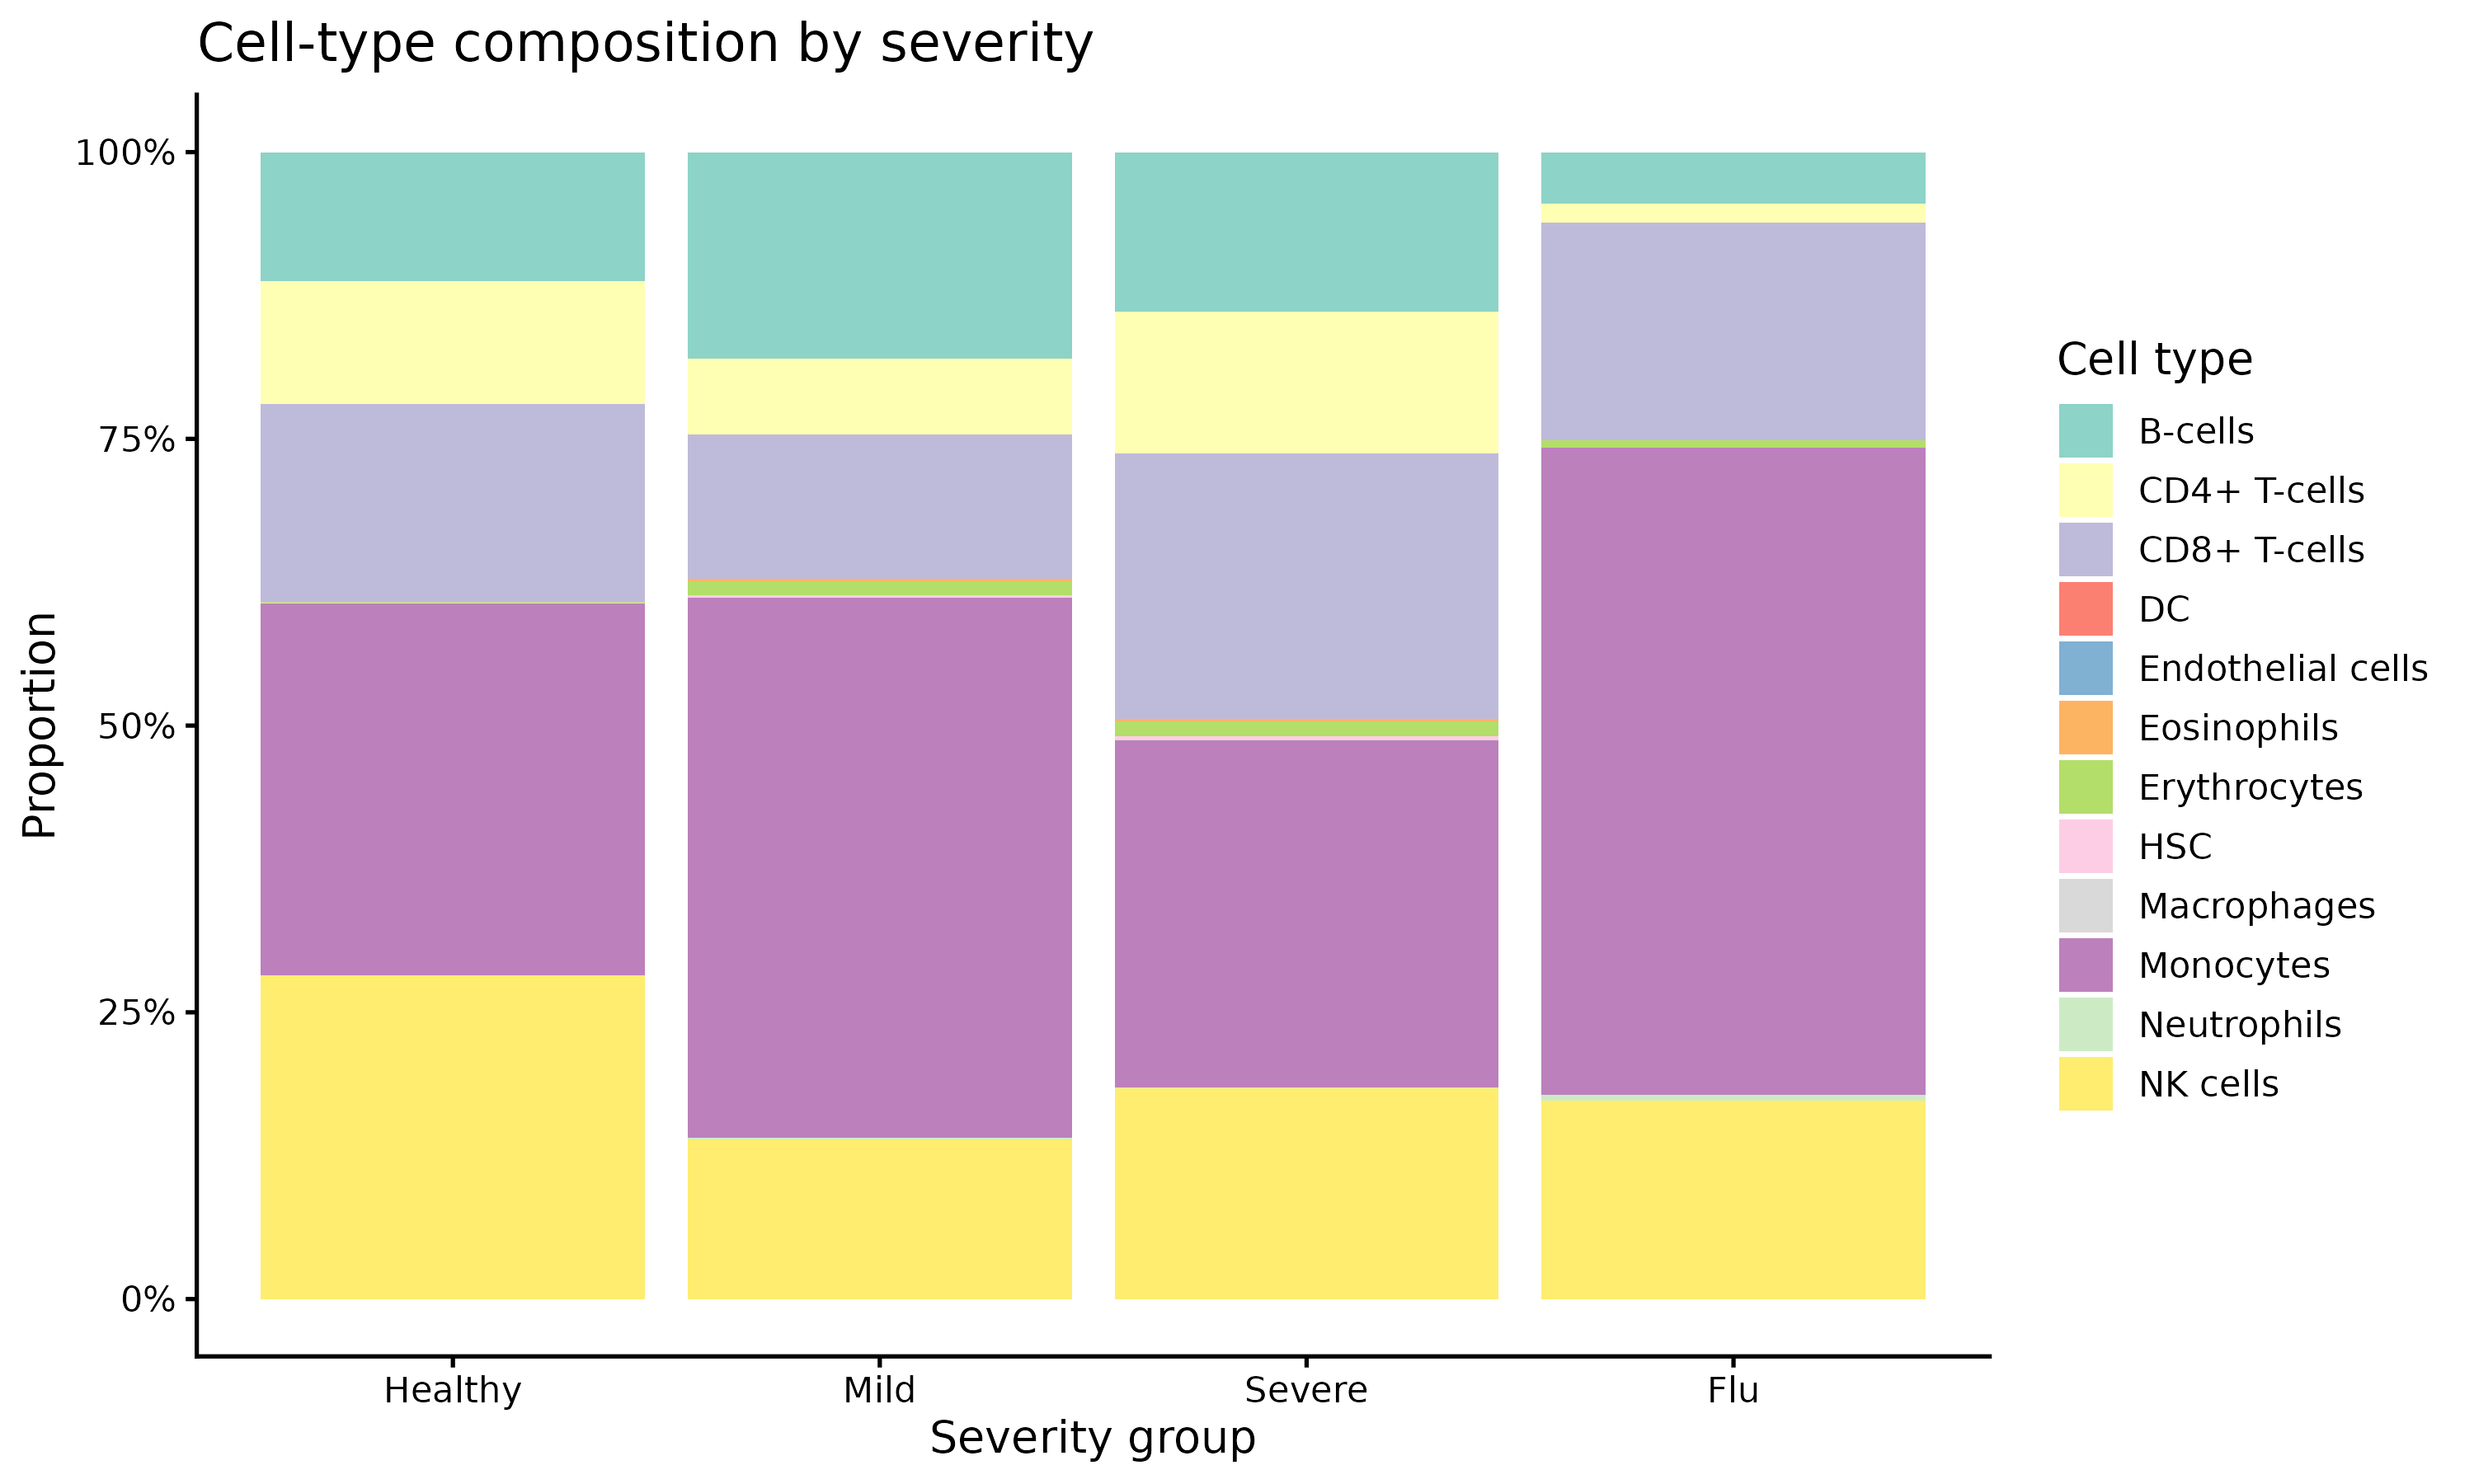
\includegraphics[width=0.85\textwidth]{plots/phase6/phase6_09_composition_barplot.png}
\end{center}

The barplot converts the visual impression into exact proportions.

\begin{itemize}[nosep]
  \item \textbf{NK cells (yellow, bottom):} Healthy $\approx$25\%, dropping steadily to
        near-zero in Flu. NK cell loss tracks disease severity.
  \item \textbf{Monocytes (purple):} Healthy $\approx$35\%, Mild $\approx$50\%,
        Severe $\approx$50\%, Flu $\approx$75\%.
        Monocyte expansion is most extreme in Flu, followed by Severe.
  \item \textbf{CD8$^+$ T-cells (lavender):} relatively stable but shrinks in Severe and Flu.
  \item \textbf{CD4$^+$ T-cells (light yellow-green):} Healthy $\approx$15\%, progressively
        smaller in Severe and Flu — \textbf{CD4$^+$ T cell depletion} is a hallmark of
        severe COVID-19 lymphopenia.
  \item \textbf{B-cells (teal, top):} present in all conditions with modest variation.
\end{itemize}

\textbf{Message:} severe COVID and especially Flu dramatically shift the blood toward monocytes
at the expense of NK and T cells. This monocyte flooding sets the stage for the inflammatory
dysregulation we measure next.

\subsection{Where are the ISG and inflammatory genes expressed?}

\subsubsection*{ISG feature plots (ISG15, IFIT1, MX1)}

\begin{center}
  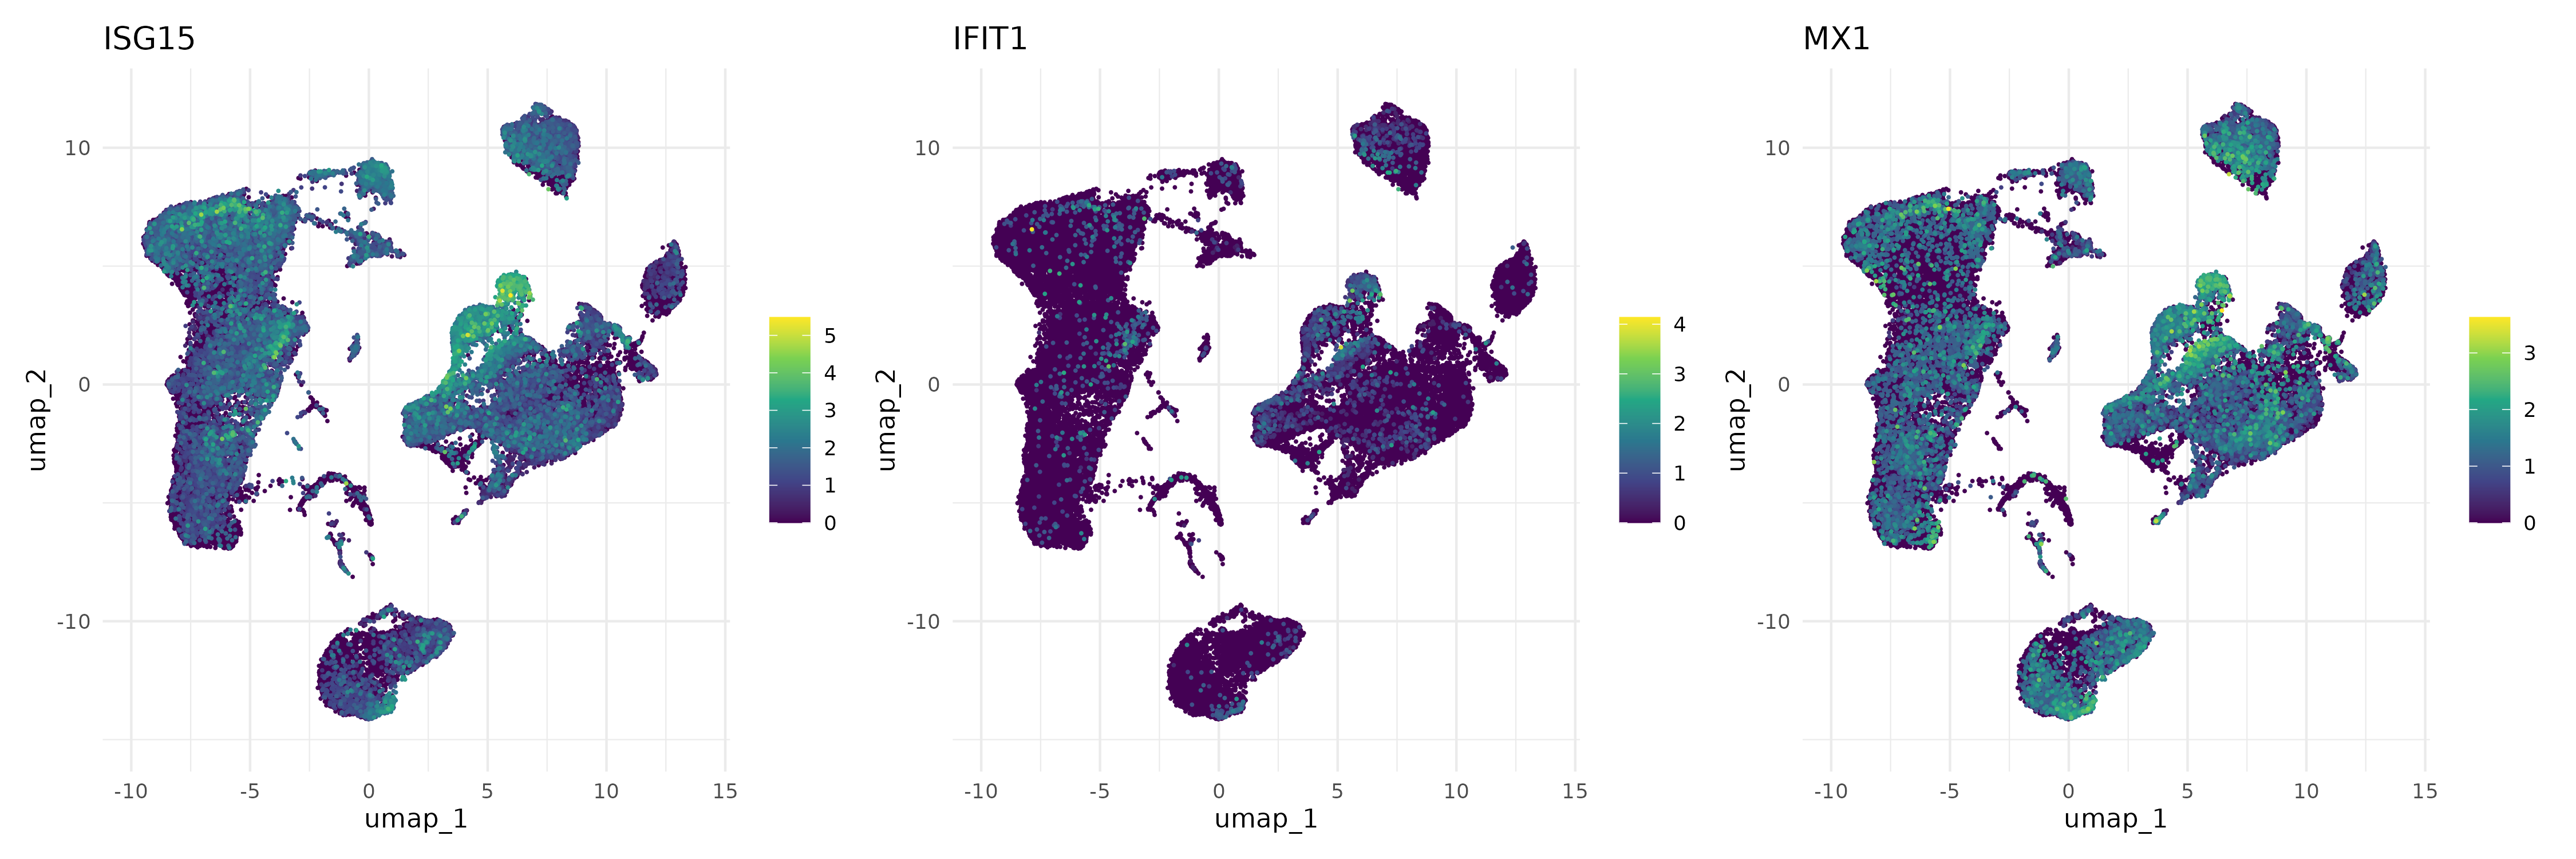
\includegraphics[width=\textwidth]{plots/phase6/phase6_03_feature_ISG.png}
\end{center}

Each plot colours every cell by the expression level of one ISG gene.
Yellow = high; dark purple = zero.

\begin{itemize}[nosep]
  \item All three ISGs (\textit{ISG15}, \textit{IFIT1}, \textit{MX1}) light up a
        \textbf{specific sub-region of the monocyte mass} on the right — consistent with
        the ISG-high monocyte cluster (Cluster 10 from Phase 3) being spatially
        distinct within the myeloid continent.
  \item ISG expression is also visible in the \textbf{isolated top cluster}
        (the small island above the main monocyte mass), confirming that this
        population is interferon-driven.
  \item The lymphoid left continent (T, NK, B cells) shows low but non-zero ISG
        expression — expected, as interferon activates all immune cells to some
        degree during infection.
  \item \textit{ISG15} has the widest expression; \textit{IFIT1} and \textit{MX1}
        are more restricted to the ISG-high monocyte sub-cluster.
\end{itemize}

\subsubsection*{TNF/IL-1$\beta$ feature plots (TNF, IL1B, CCL3)}

\begin{center}
  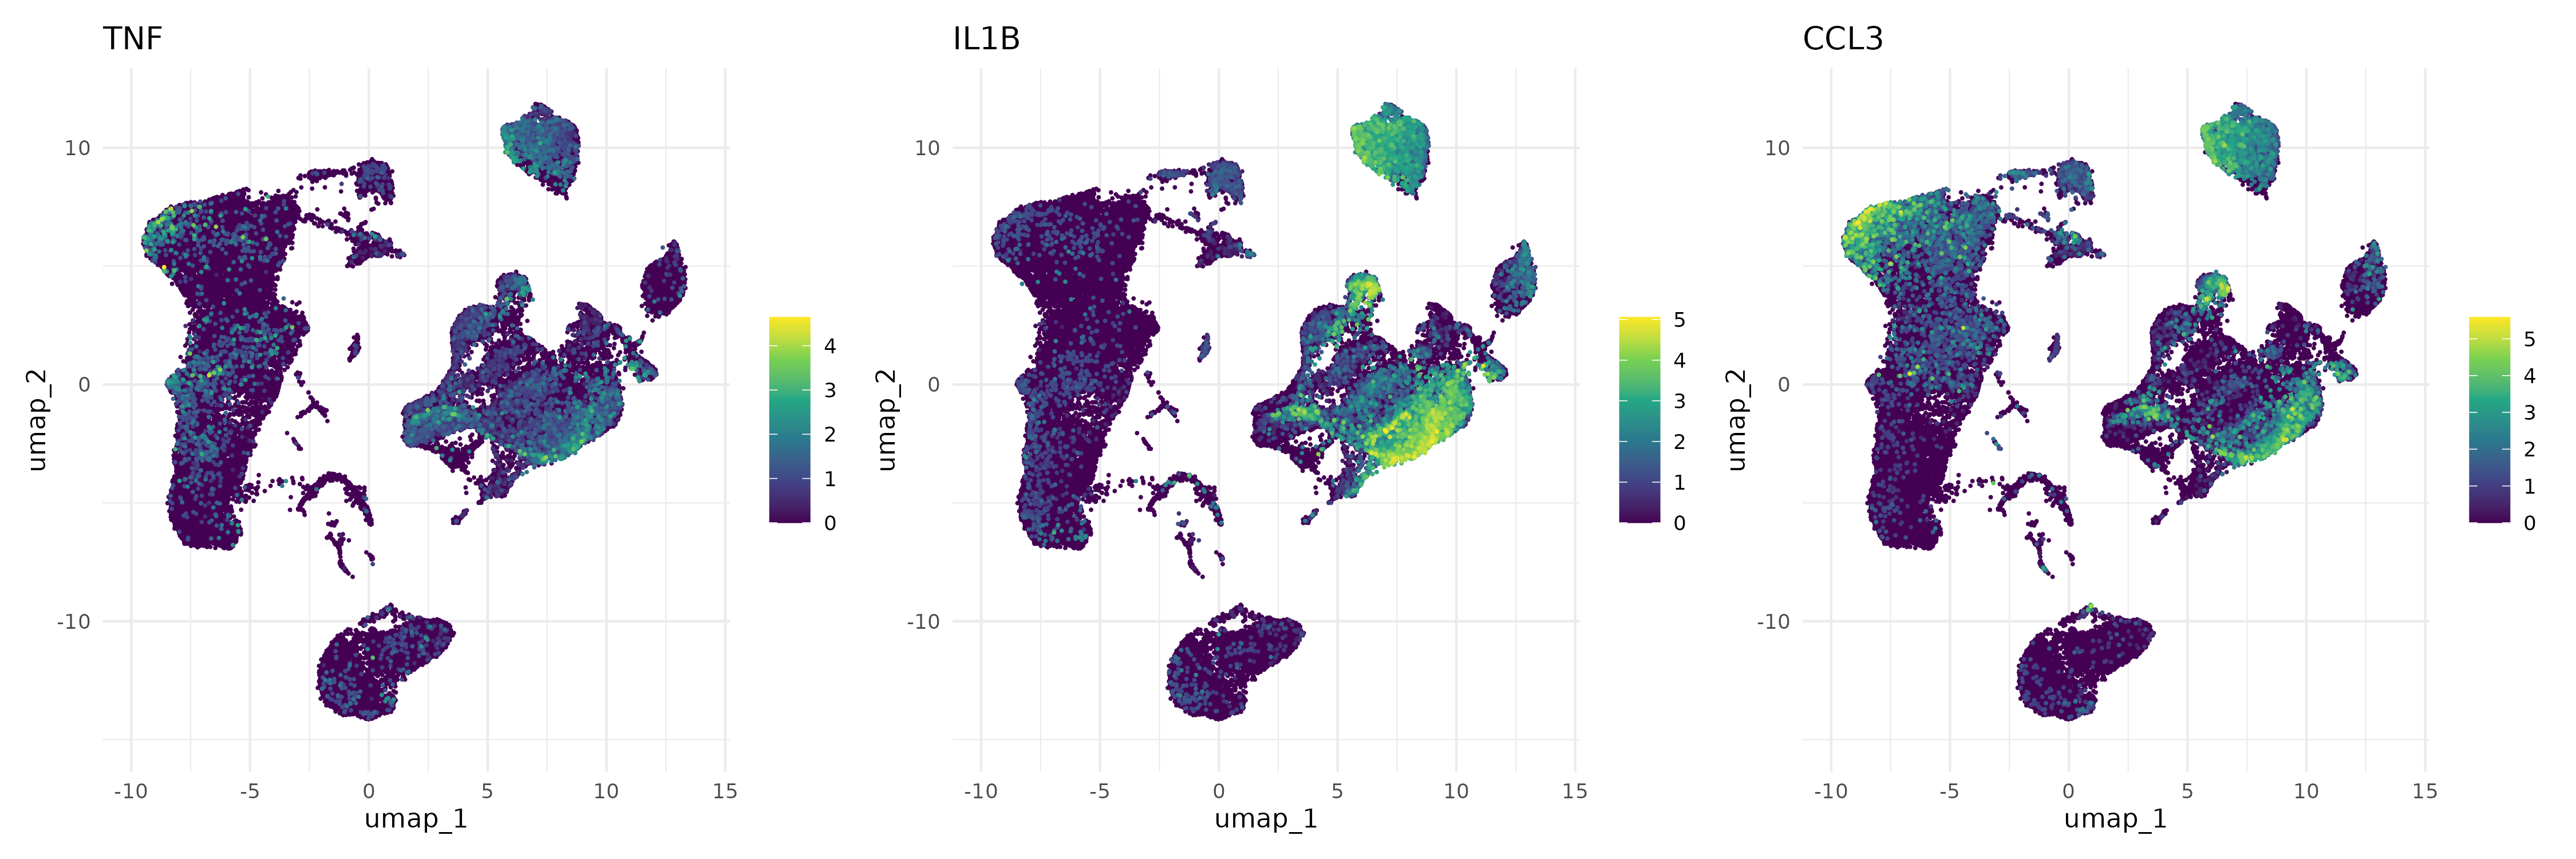
\includegraphics[width=\textwidth]{plots/phase6/phase6_04_feature_TNF_IL1.png}
\end{center}

\begin{itemize}[nosep]
  \item \textit{IL1B} is the most striking: a \textbf{bright yellow core} lights up a
        specific sub-region within the monocyte mass, corresponding precisely to
        Cluster 7 (IL-1$\beta^+$ inflammasome-active monocytes from Phase 3).
        Virtually no expression outside that cluster.
  \item \textit{CCL3} spreads more broadly across the monocyte mass —
        it is expressed at moderate levels throughout the myeloid continent, indicating
        that chemokine production is a general monocyte feature, not sub-cluster-specific.
  \item \textit{TNF} expression is detectable but more diffuse, consistent with TNF
        being produced at lower levels across a wider range of activated cells.
  \item The lymphoid continent is essentially dark for all three genes —
        TNF/IL-1$\beta$ activity is \textbf{myeloid-specific} in this dataset.
\end{itemize}

\textbf{Taken together:} the ISG and inflammatory programs live in \textit{different
spatial locations} within the monocyte mass on the UMAP. This spatial separation
is why co-activation (both programs on in the same cell) is the
interesting finding — most cells have one or neither program active.

\subsection{Module scores and co-activation}

\subsubsection*{Violin plots — module scores by severity}

\begin{center}
  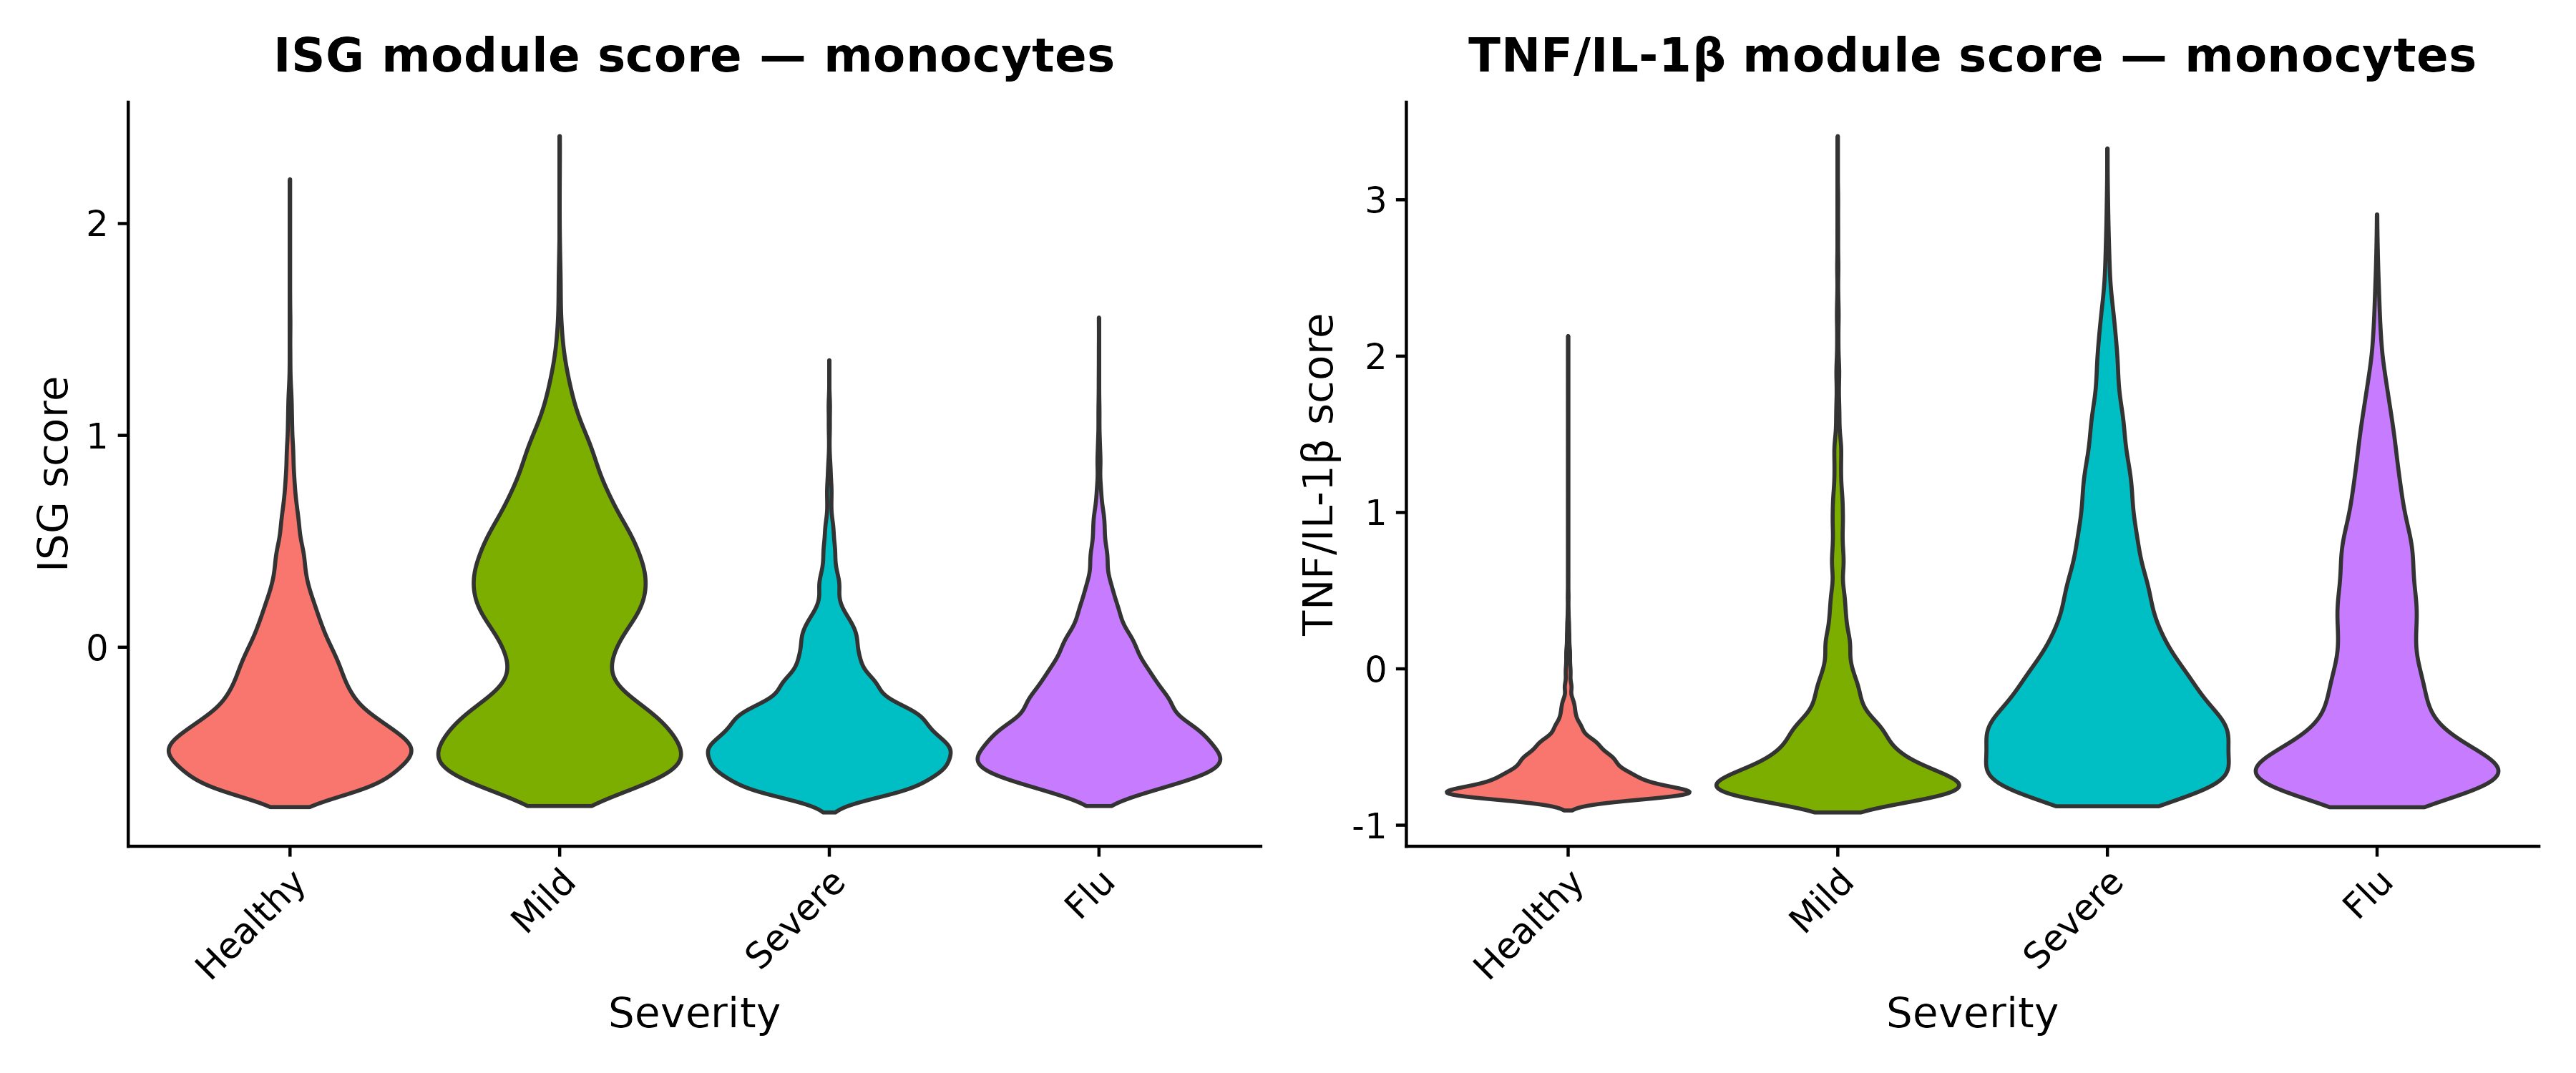
\includegraphics[width=\textwidth]{plots/phase6/phase6_05_violin_module_scores.png}
\end{center}

\textit{Left — ISG score:}
\begin{itemize}[nosep]
  \item \textbf{Healthy:} narrow, centered near $-0.5$. ISG program is off.
  \item \textbf{Mild:} wide, bimodal shape — two sub-populations of monocytes, one
        with the ISG program partially on and one without.
        \textbf{Mild COVID drives the strongest ISG response at the cell level.}
  \item \textbf{Severe:} relatively narrow, centered near $-0.5$. Similar to Healthy.
        The ISG program is not broadly active in severe COVID monocytes.
  \item \textbf{Flu:} narrow, similar to Severe and Healthy.
\end{itemize}

\textit{Right — TNF/IL-1$\beta$ score:}
\begin{itemize}[nosep]
  \item \textbf{Healthy:} tight mass at $-1$. Program is silent.
  \item \textbf{Mild:} slightly wider, still mostly low.
  \item \textbf{Severe:} \textbf{markedly wider and taller} — extends to $\approx +3$.
        A large fraction of severe COVID monocytes actively run the inflammatory program.
  \item \textbf{Flu:} similarly wide, multi-peaked — monocytes span a range of
        inflammatory states.
\end{itemize}

The contrast is the key message: \textbf{Mild COVID = ISG-dominant; Severe COVID = inflammation-dominant.}
The programs are not co-elevated in the same group — they shift in opposite directions as
disease worsens.

\subsubsection*{Donor co-activation boxplot}

\begin{center}
  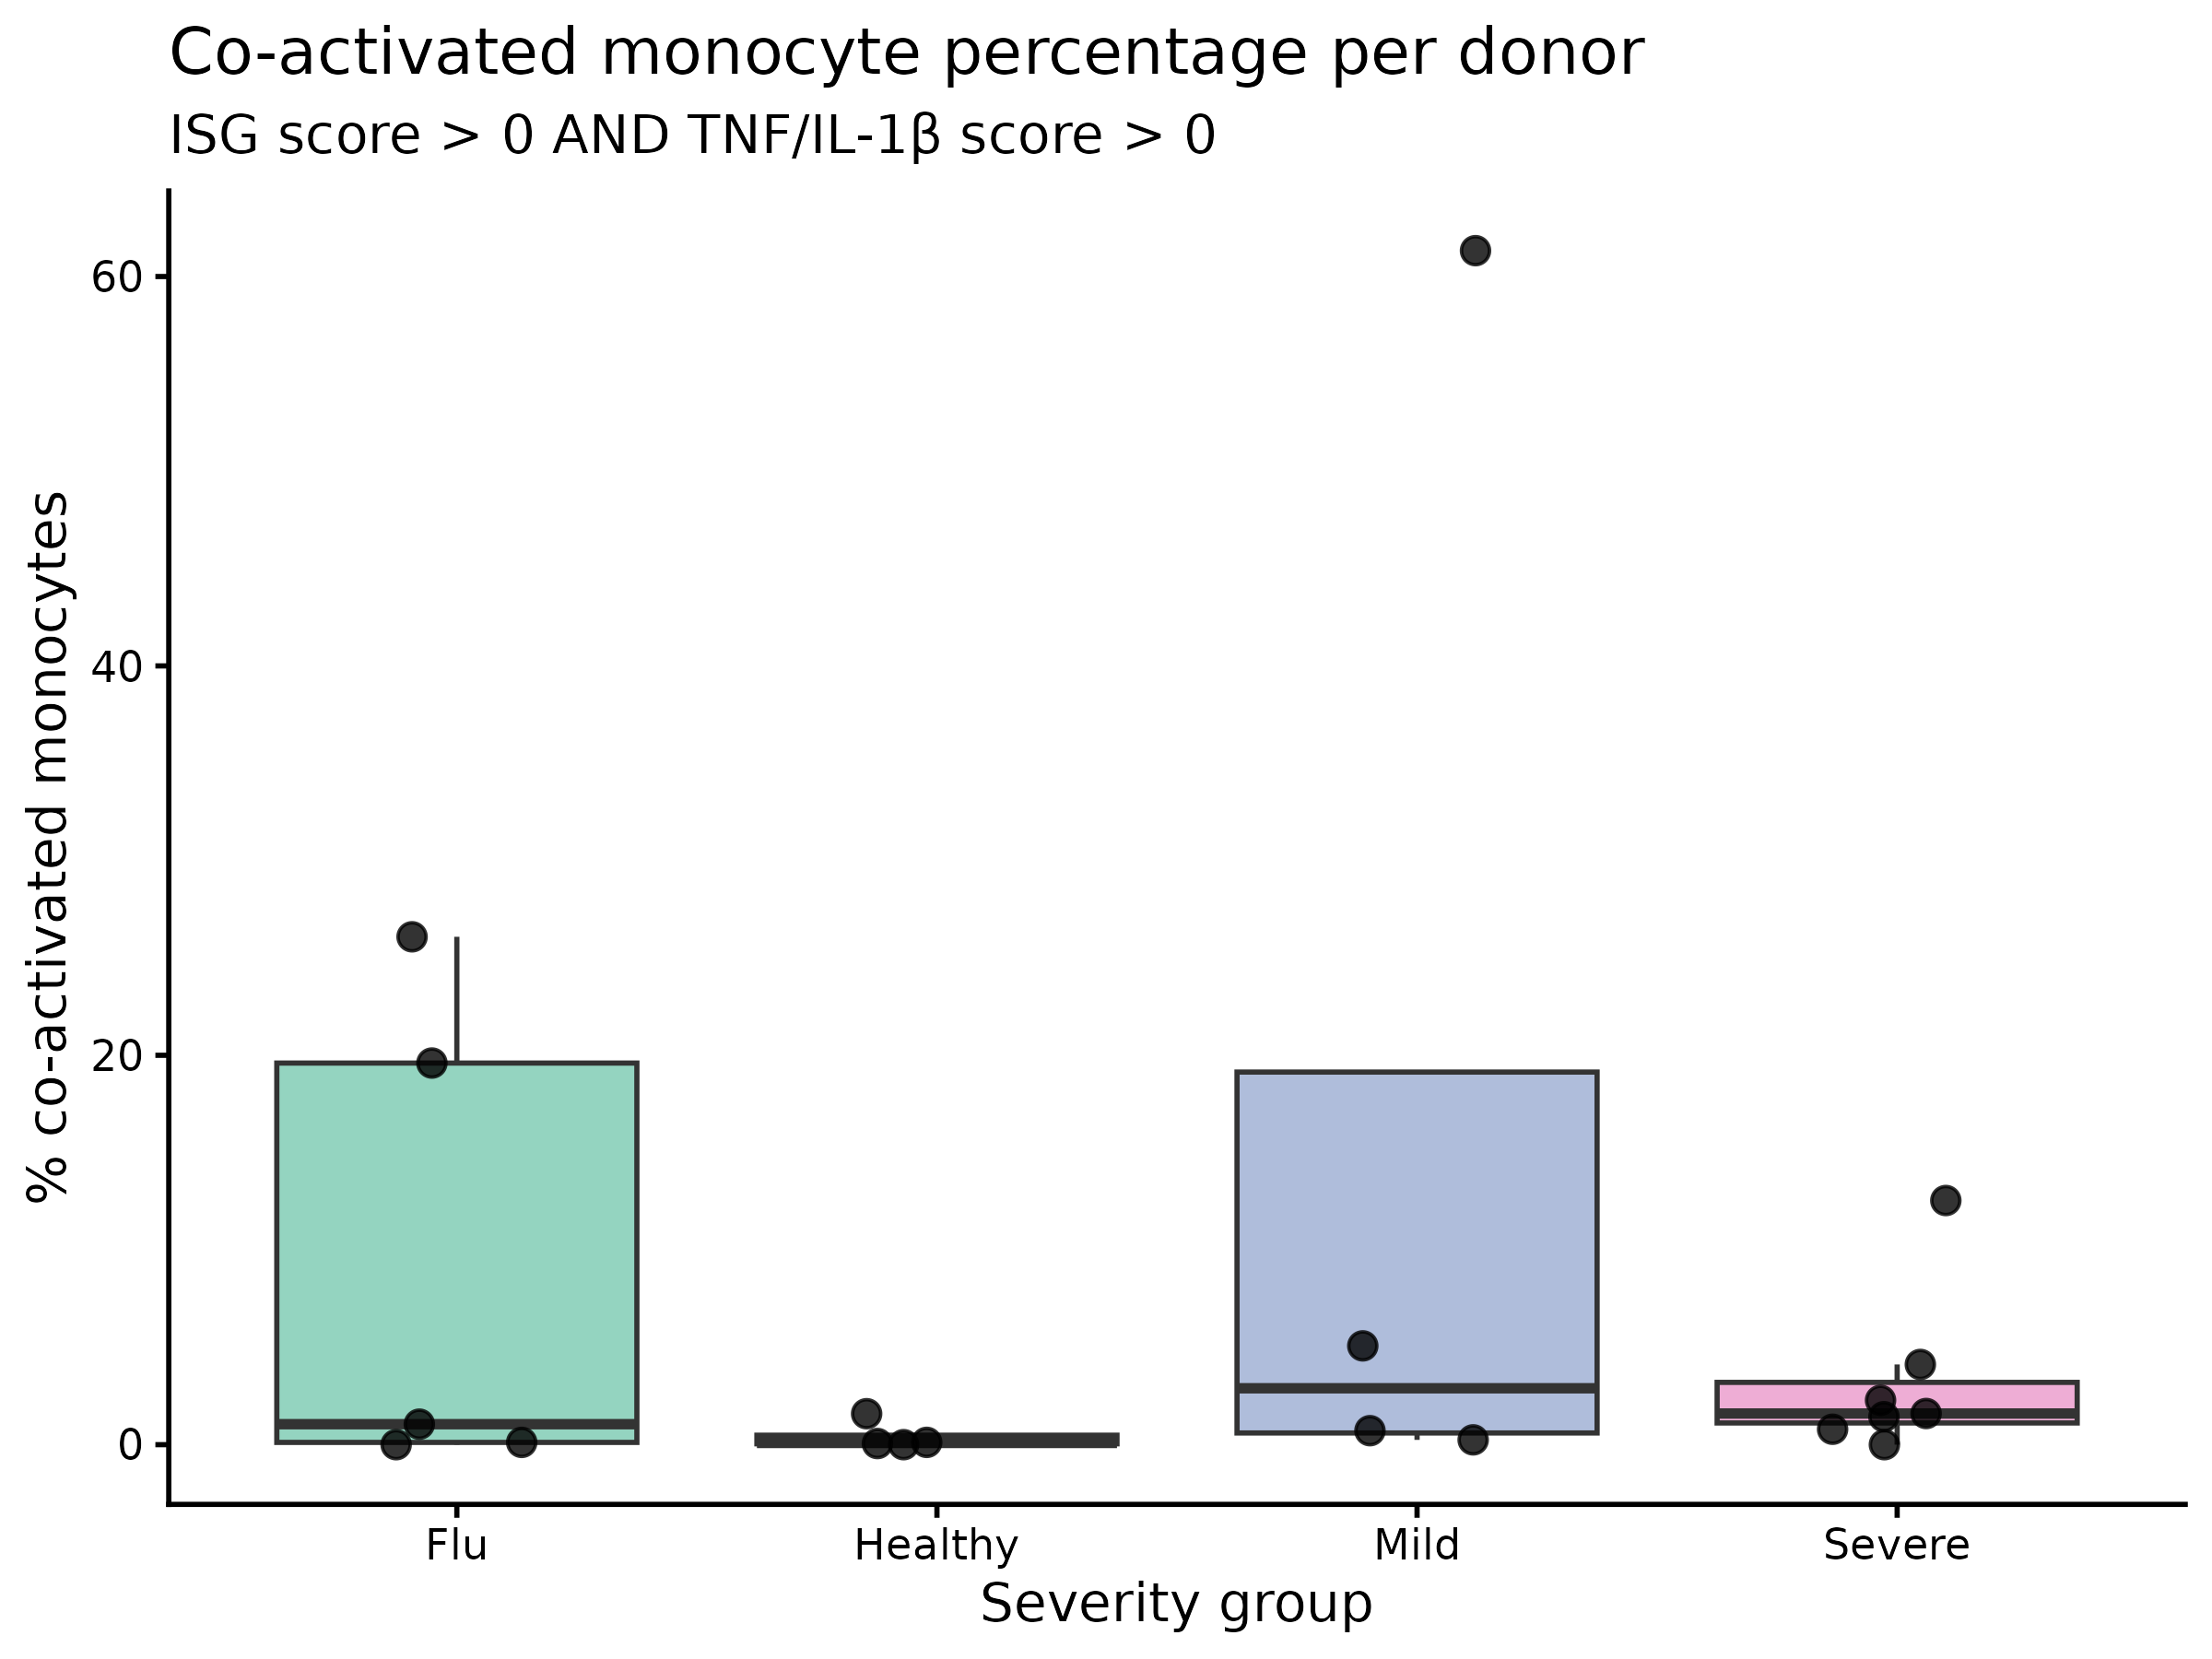
\includegraphics[width=0.85\textwidth]{plots/phase6/phase6_06_donor_coactivation_boxplot.png}
\end{center}

Each dot is one donor; the y-axis is the percentage of that donor's monocytes that are
co-activated (both ISG $>0$ and TNF/IL-1$\beta >0$ simultaneously).

\begin{itemize}[nosep]
  \item \textbf{Healthy:} all donors cluster near 0\%. Resting monocytes are never co-activated.
  \item \textbf{Mild:} wide spread. Most donors are in the 0–5\% range, but
        \textbf{one outlier donor reaches $\approx$61\%} — an extraordinary co-activation
        rate suggesting that individual mild-disease patients can mount an unusually
        strong dual response.
  \item \textbf{Severe:} tight cluster, mostly 0–5\% with one outlier near 13\%.
        Counter-intuitively, the \textit{median} co-activation rate in Severe is actually
        \textit{lower} than in Mild. The severe state shifts monocytes toward pure inflammation
        (top-left quadrant) rather than dual co-activation.
  \item \textbf{Flu:} the highest and most consistent co-activation, with a median
        near $\approx$20\% and several donors above 20\%.
\end{itemize}

\textbf{Key nuance:} co-activation rate does not simply increase with disease severity.
Flu has the highest co-activation; Severe COVID monocytes are highly inflamed but their
ISG response is relatively suppressed, pushing them out of the co-activated quadrant into
the ``pure inflammation'' quadrant.

\subsection{Differential expression volcano}

\begin{center}
  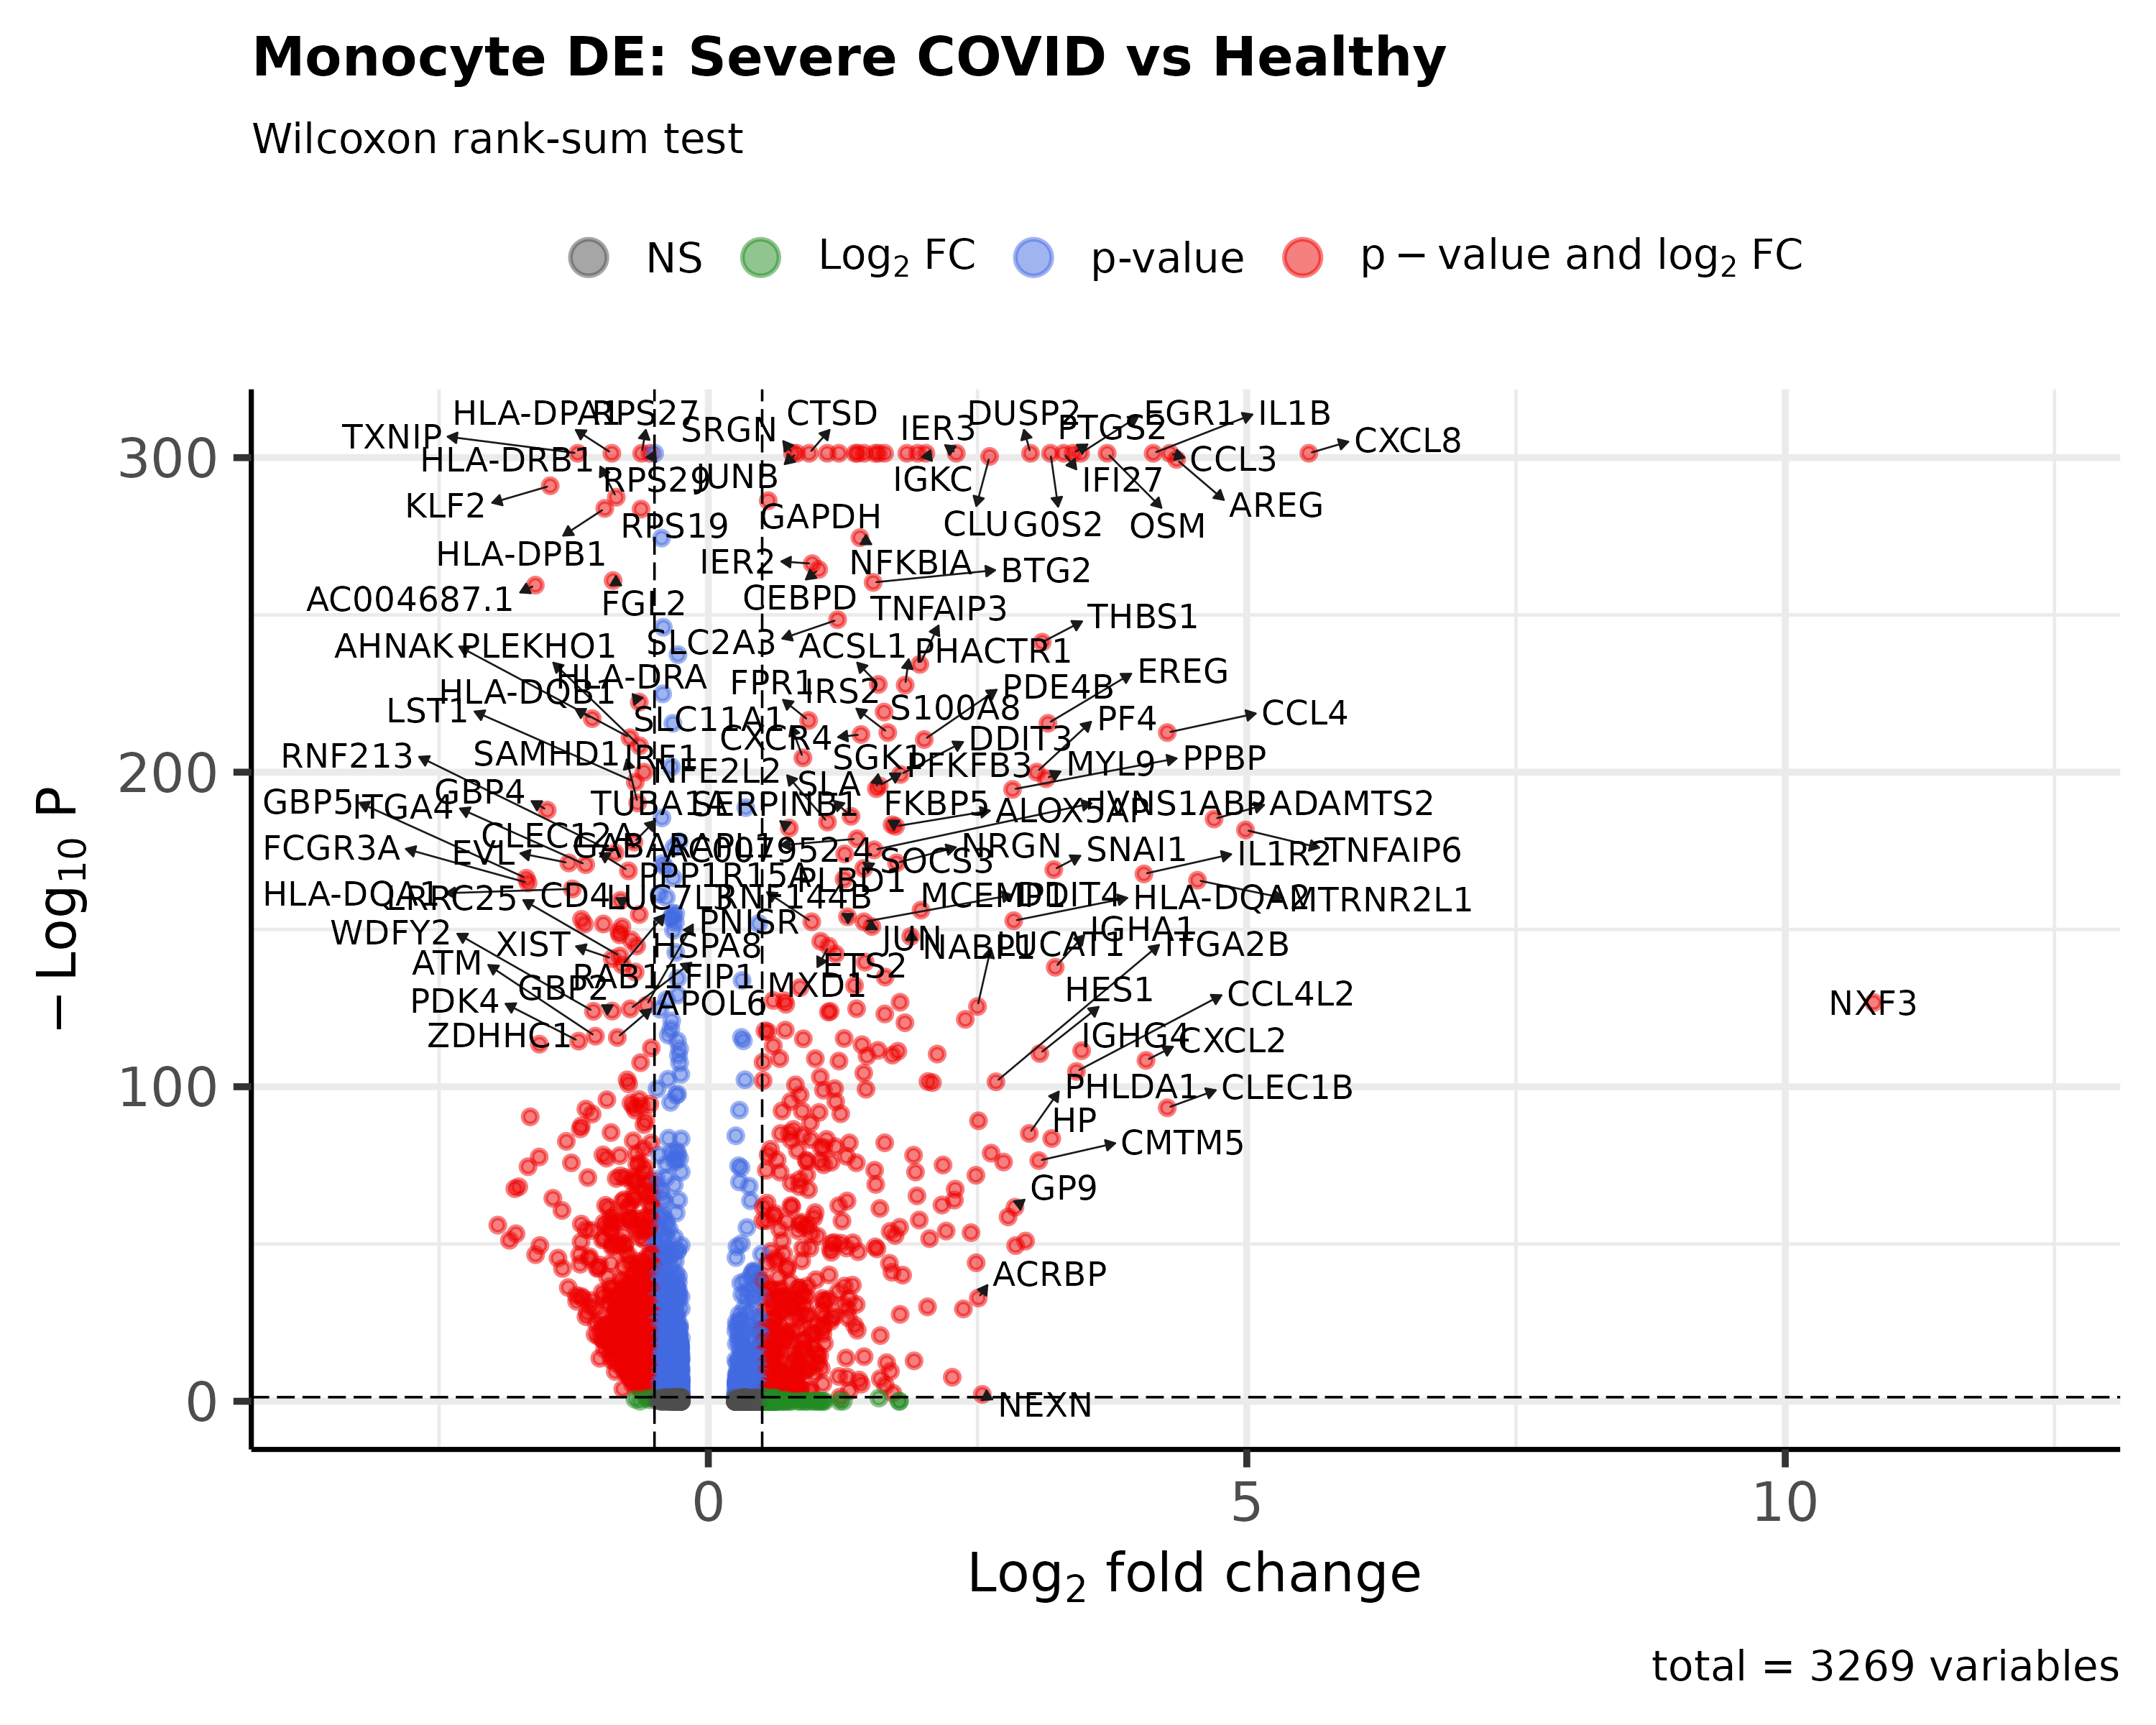
\includegraphics[width=0.95\textwidth]{plots/phase6/phase6_07_volcano_monocyte_DE.png}
\end{center}

Severe COVID monocytes vs Healthy monocytes; 3,269 significantly DE genes.
This is the same analysis as Phase 4, here presented in final plotting style.

Key genes visible:
\begin{itemize}[nosep]
  \item \textbf{Top upregulated (top-right):} \textit{IL1B}, \textit{CXCL8}, \textit{CCL3},
        \textit{OSM}, \textit{PTGS2} — the core inflammatory program.
        \textit{NFKBIA} and \textit{TNFAIP3} also appear — negative feedback regulators
        of NF-$\kappa$B trying to brake the response.
  \item \textbf{Top downregulated (top-left):} \textit{TXNIP}, \textit{KLF2},
        \textit{HLA-DPA1}, \textit{HLA-DRB1}, \textit{HLA-DQB1} — loss of the cell's
        homeostatic identity and antigen-presentation capacity.
  \item \textbf{Outlier (far right):} \textit{NXF3} at $\log_2$FC $\approx 11$,
        an RNA export factor of unclear COVID relevance.
\end{itemize}

Severe COVID monocytes are not simply ``activated'' — they gain a massive inflammatory output
while simultaneously losing their ability to present antigens to T cells (HLA downregulation).
This dual change (gain inflammation + lose function) is the molecular definition of the
pathological monocyte reprogramming seen in severe COVID.

\subsection{Cluster marker heatmap}

\begin{center}
  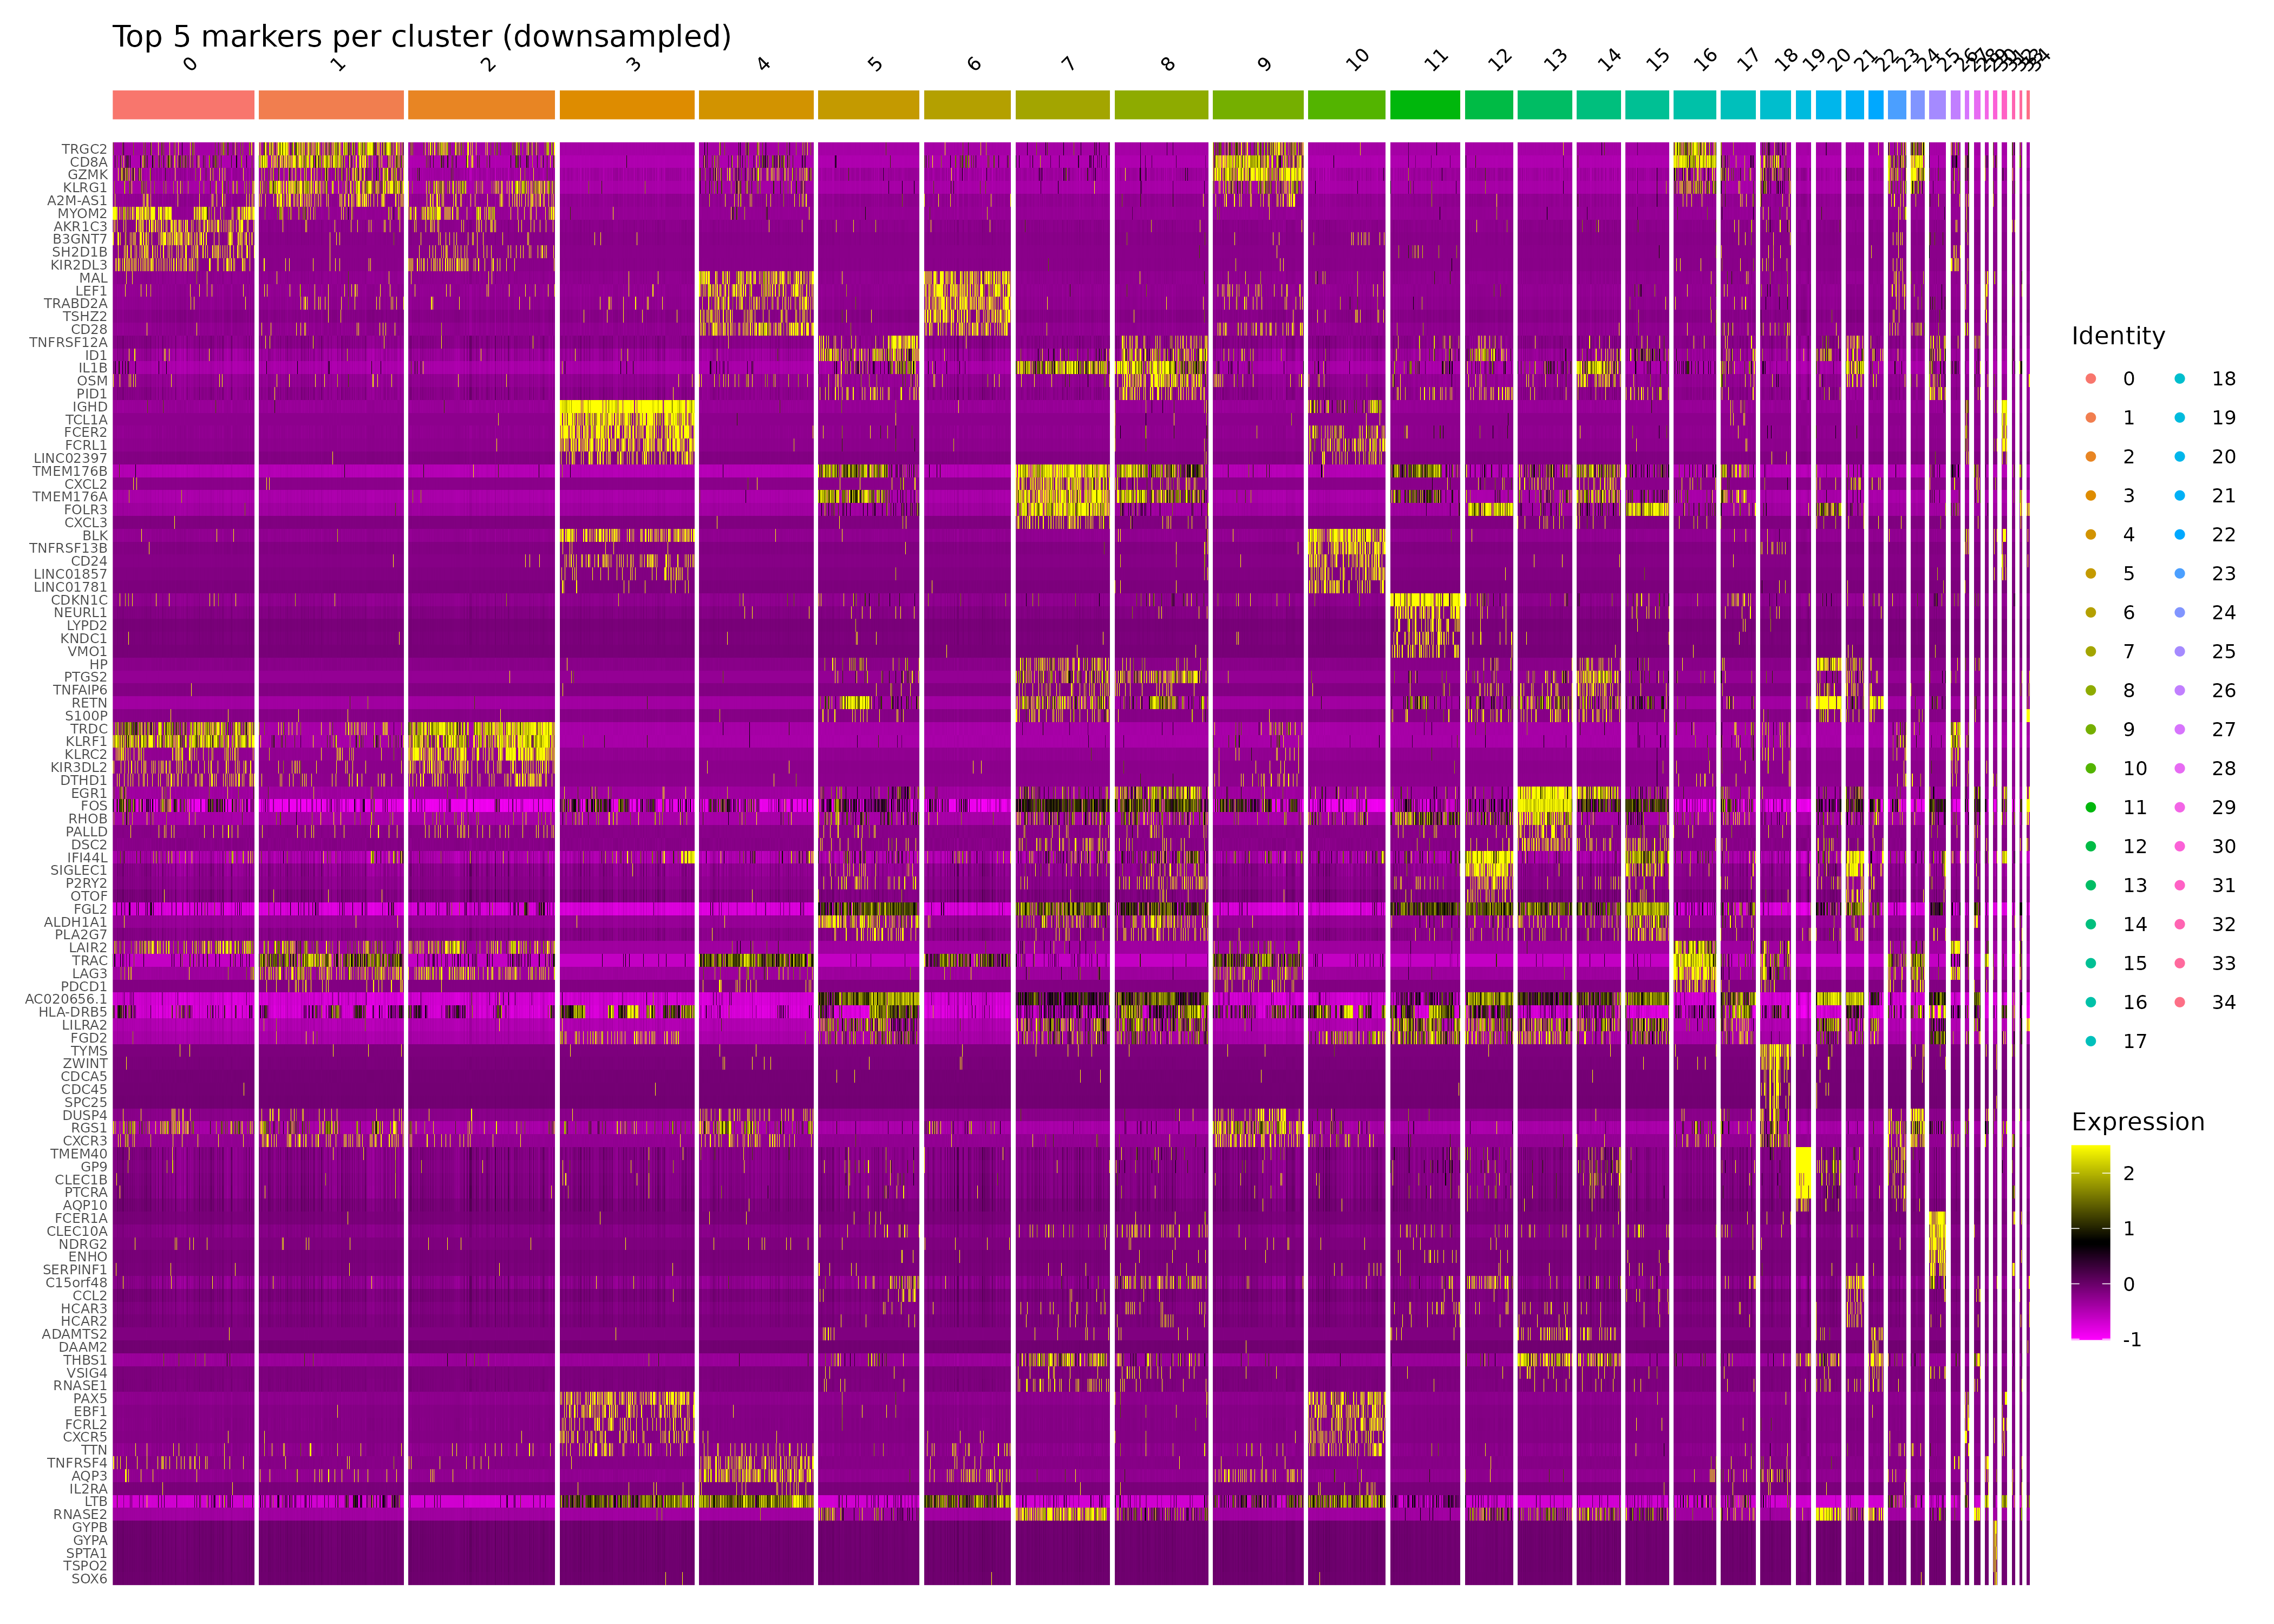
\includegraphics[width=\textwidth]{plots/phase6/phase6_08_marker_heatmap.png}
\end{center}

Top 5 marker genes per cluster across all 35 clusters (the expanded final object).
Yellow = high expression; purple = low.

The heatmap shows a clean diagonal structure: each gene block lights up in one cluster
and is dark everywhere else, confirming that the cluster boundaries found by Louvain
correspond to genuinely distinct transcriptional programs.
Notable sub-clusters visible in this expanded view:
\begin{itemize}[nosep]
  \item Multiple monocyte sub-clusters (mid-right of the heatmap), each with distinct
        marker genes, confirming the diversity of monocyte states described in Phase 3.
  \item Clear T cell sub-clusters on the left of the heatmap, with \textit{CD8A}, \textit{GZMK},
        \textit{LEF1}, and \textit{IL7R} separating effector memory, naive, and helper sub-types.
  \item A compact isolated NK cluster with \textit{PRF1} and \textit{KIR} family genes.
  \item The B cell cluster block with \textit{MS4A1}, \textit{CD79A}, and immunoglobulin genes.
\end{itemize}

\subsection{Replication in GSE150861}

\begin{center}
  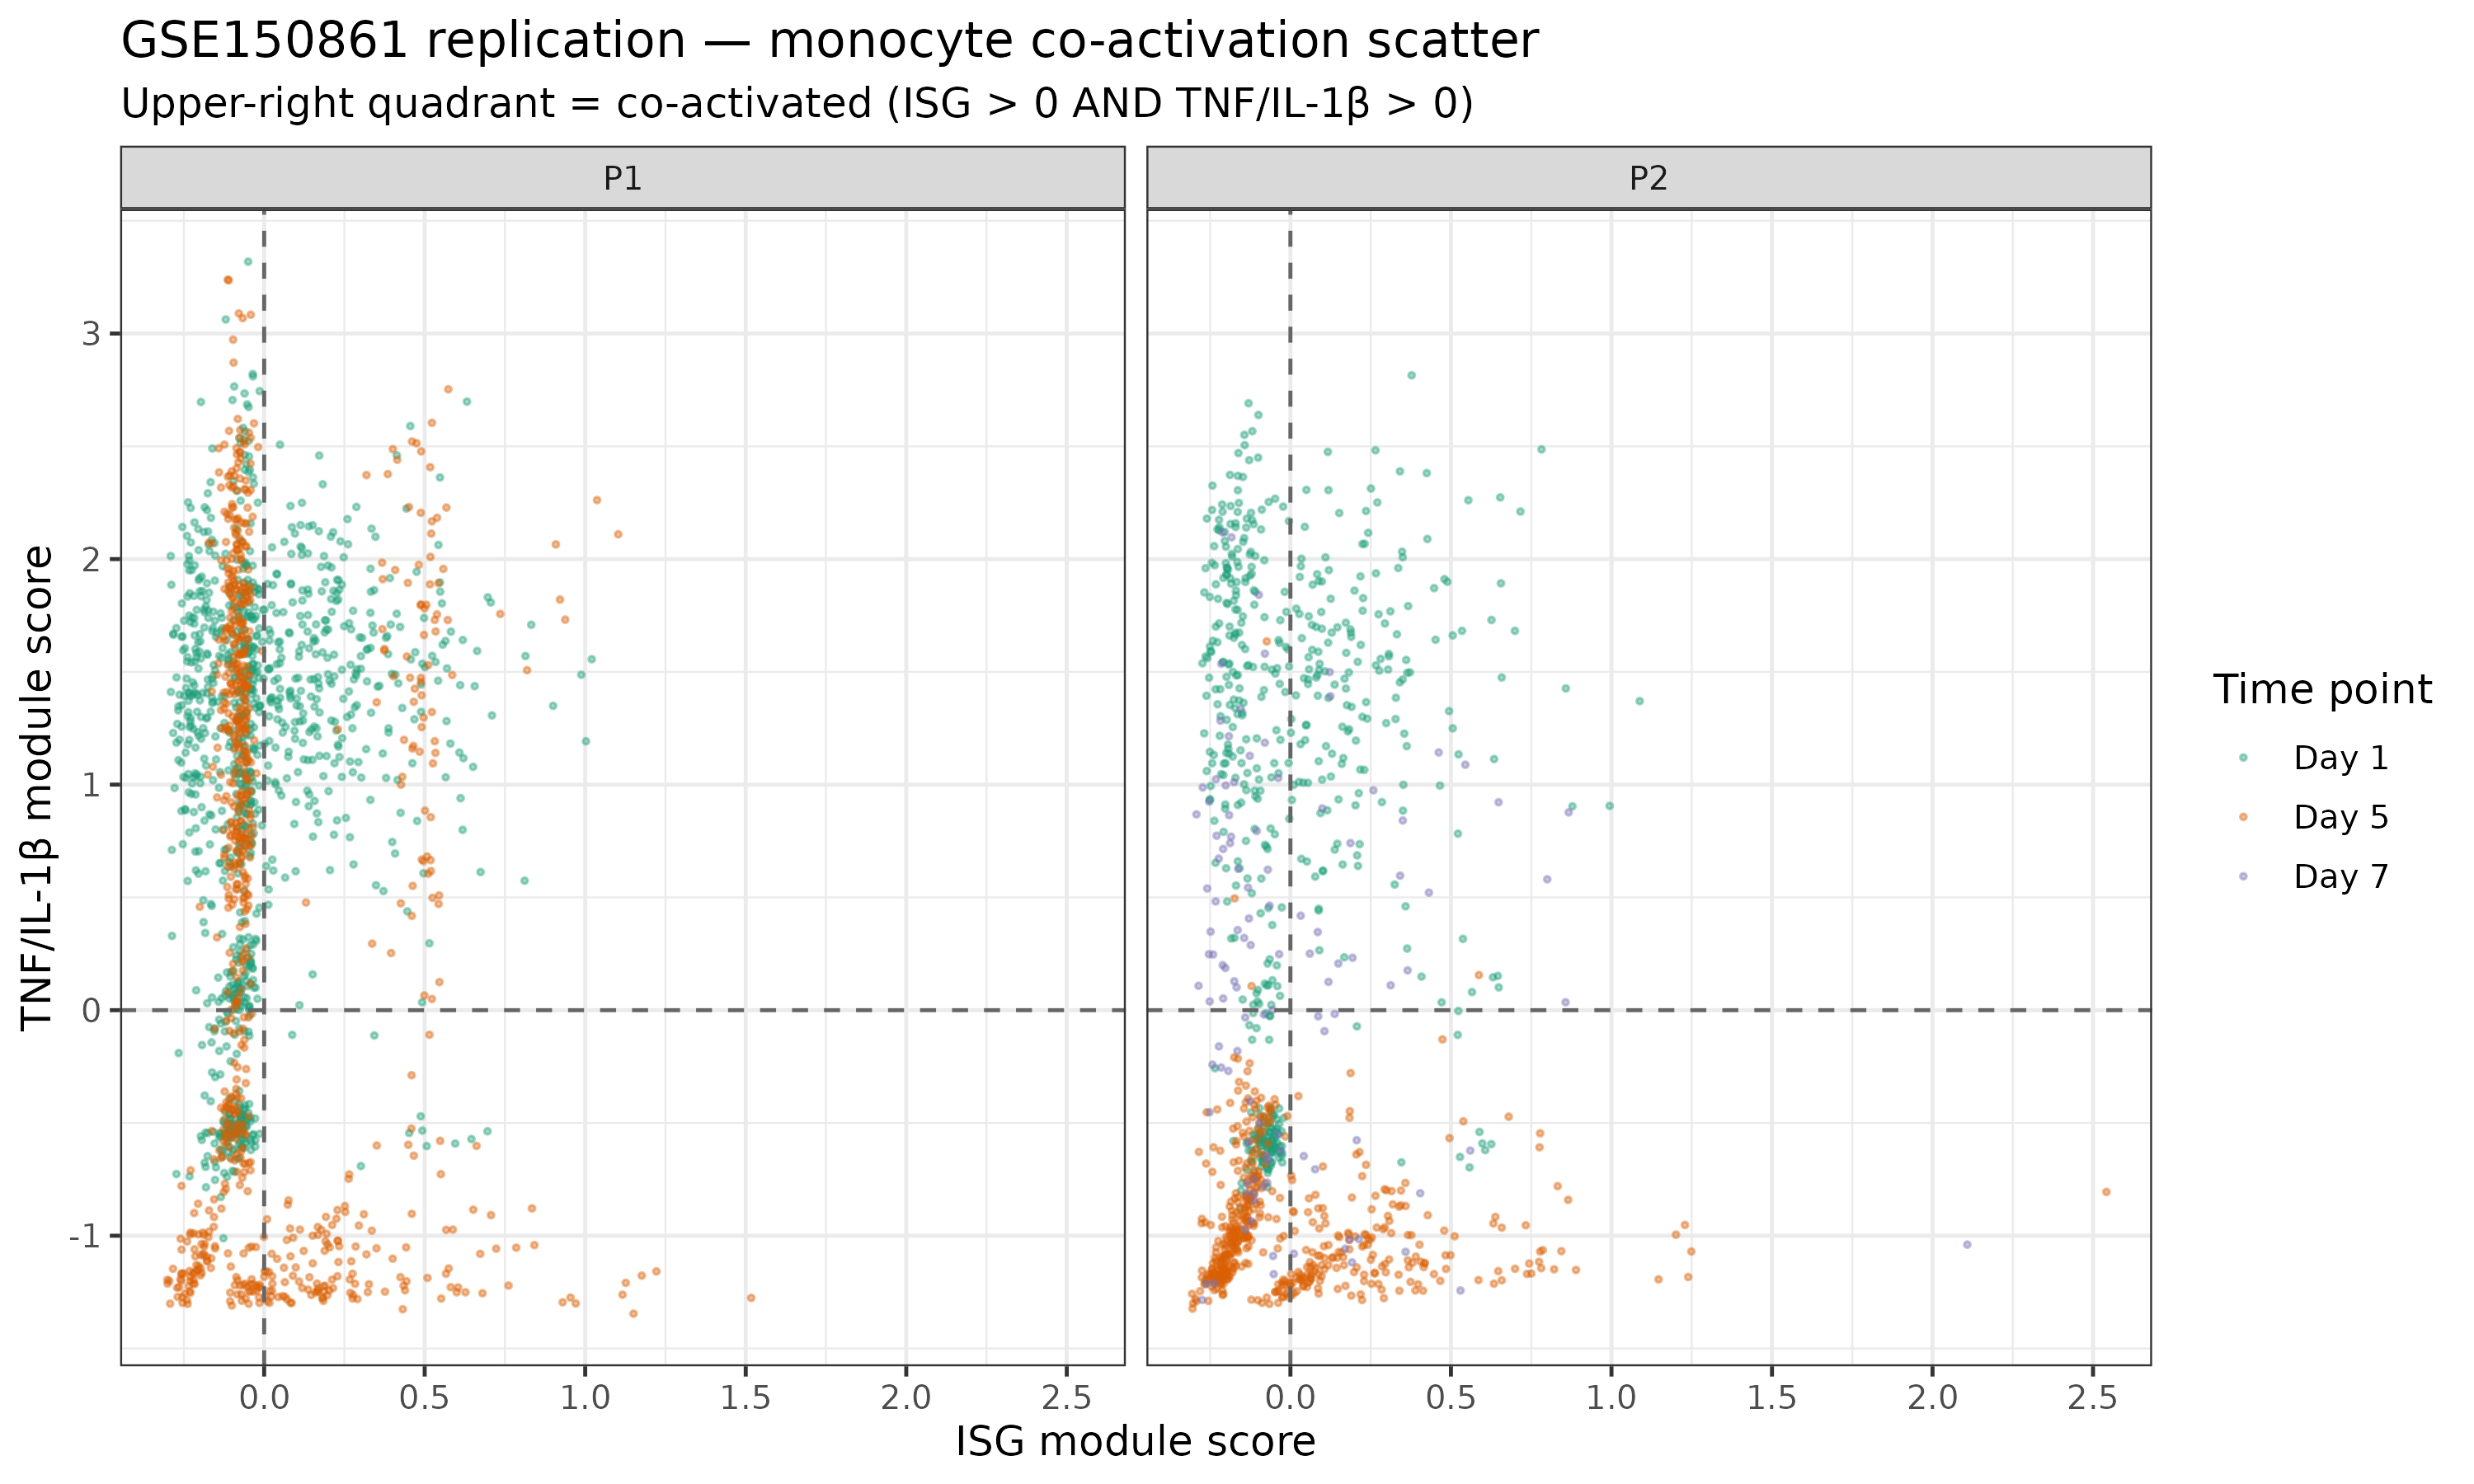
\includegraphics[width=\textwidth]{plots/phase6/phase6_10_replication_coactivation.png}
\end{center}

The co-activation scatter from Phase 5, presented in final style.
Each dot is one monocyte from GSE150861; colour = time point.

Key observations (same as Phase 5):
\begin{itemize}[nosep]
  \item \textbf{Day 1 (teal/green):} both P1 and P2 show monocytes in the top-right
        (co-activated) quadrant. The co-activated state is confirmed in both patients.
  \item \textbf{Day 5 (orange):} cells shift downward — the TNF/IL-1$\beta$ component
        drops as Tocilizumab suppresses inflammation. Fewer cells in the top quadrants.
  \item \textbf{Day 7 (purple):} monocytes are scarce and mostly in the lower half.
        The inflammatory program is further reduced.
  \item P2 shows a tighter ISG-near-zero pattern compared to P1's wider spread —
        patient-to-patient variability is real and present even within the same condition.
\end{itemize}

\subsection{Summary panel}

\begin{center}
  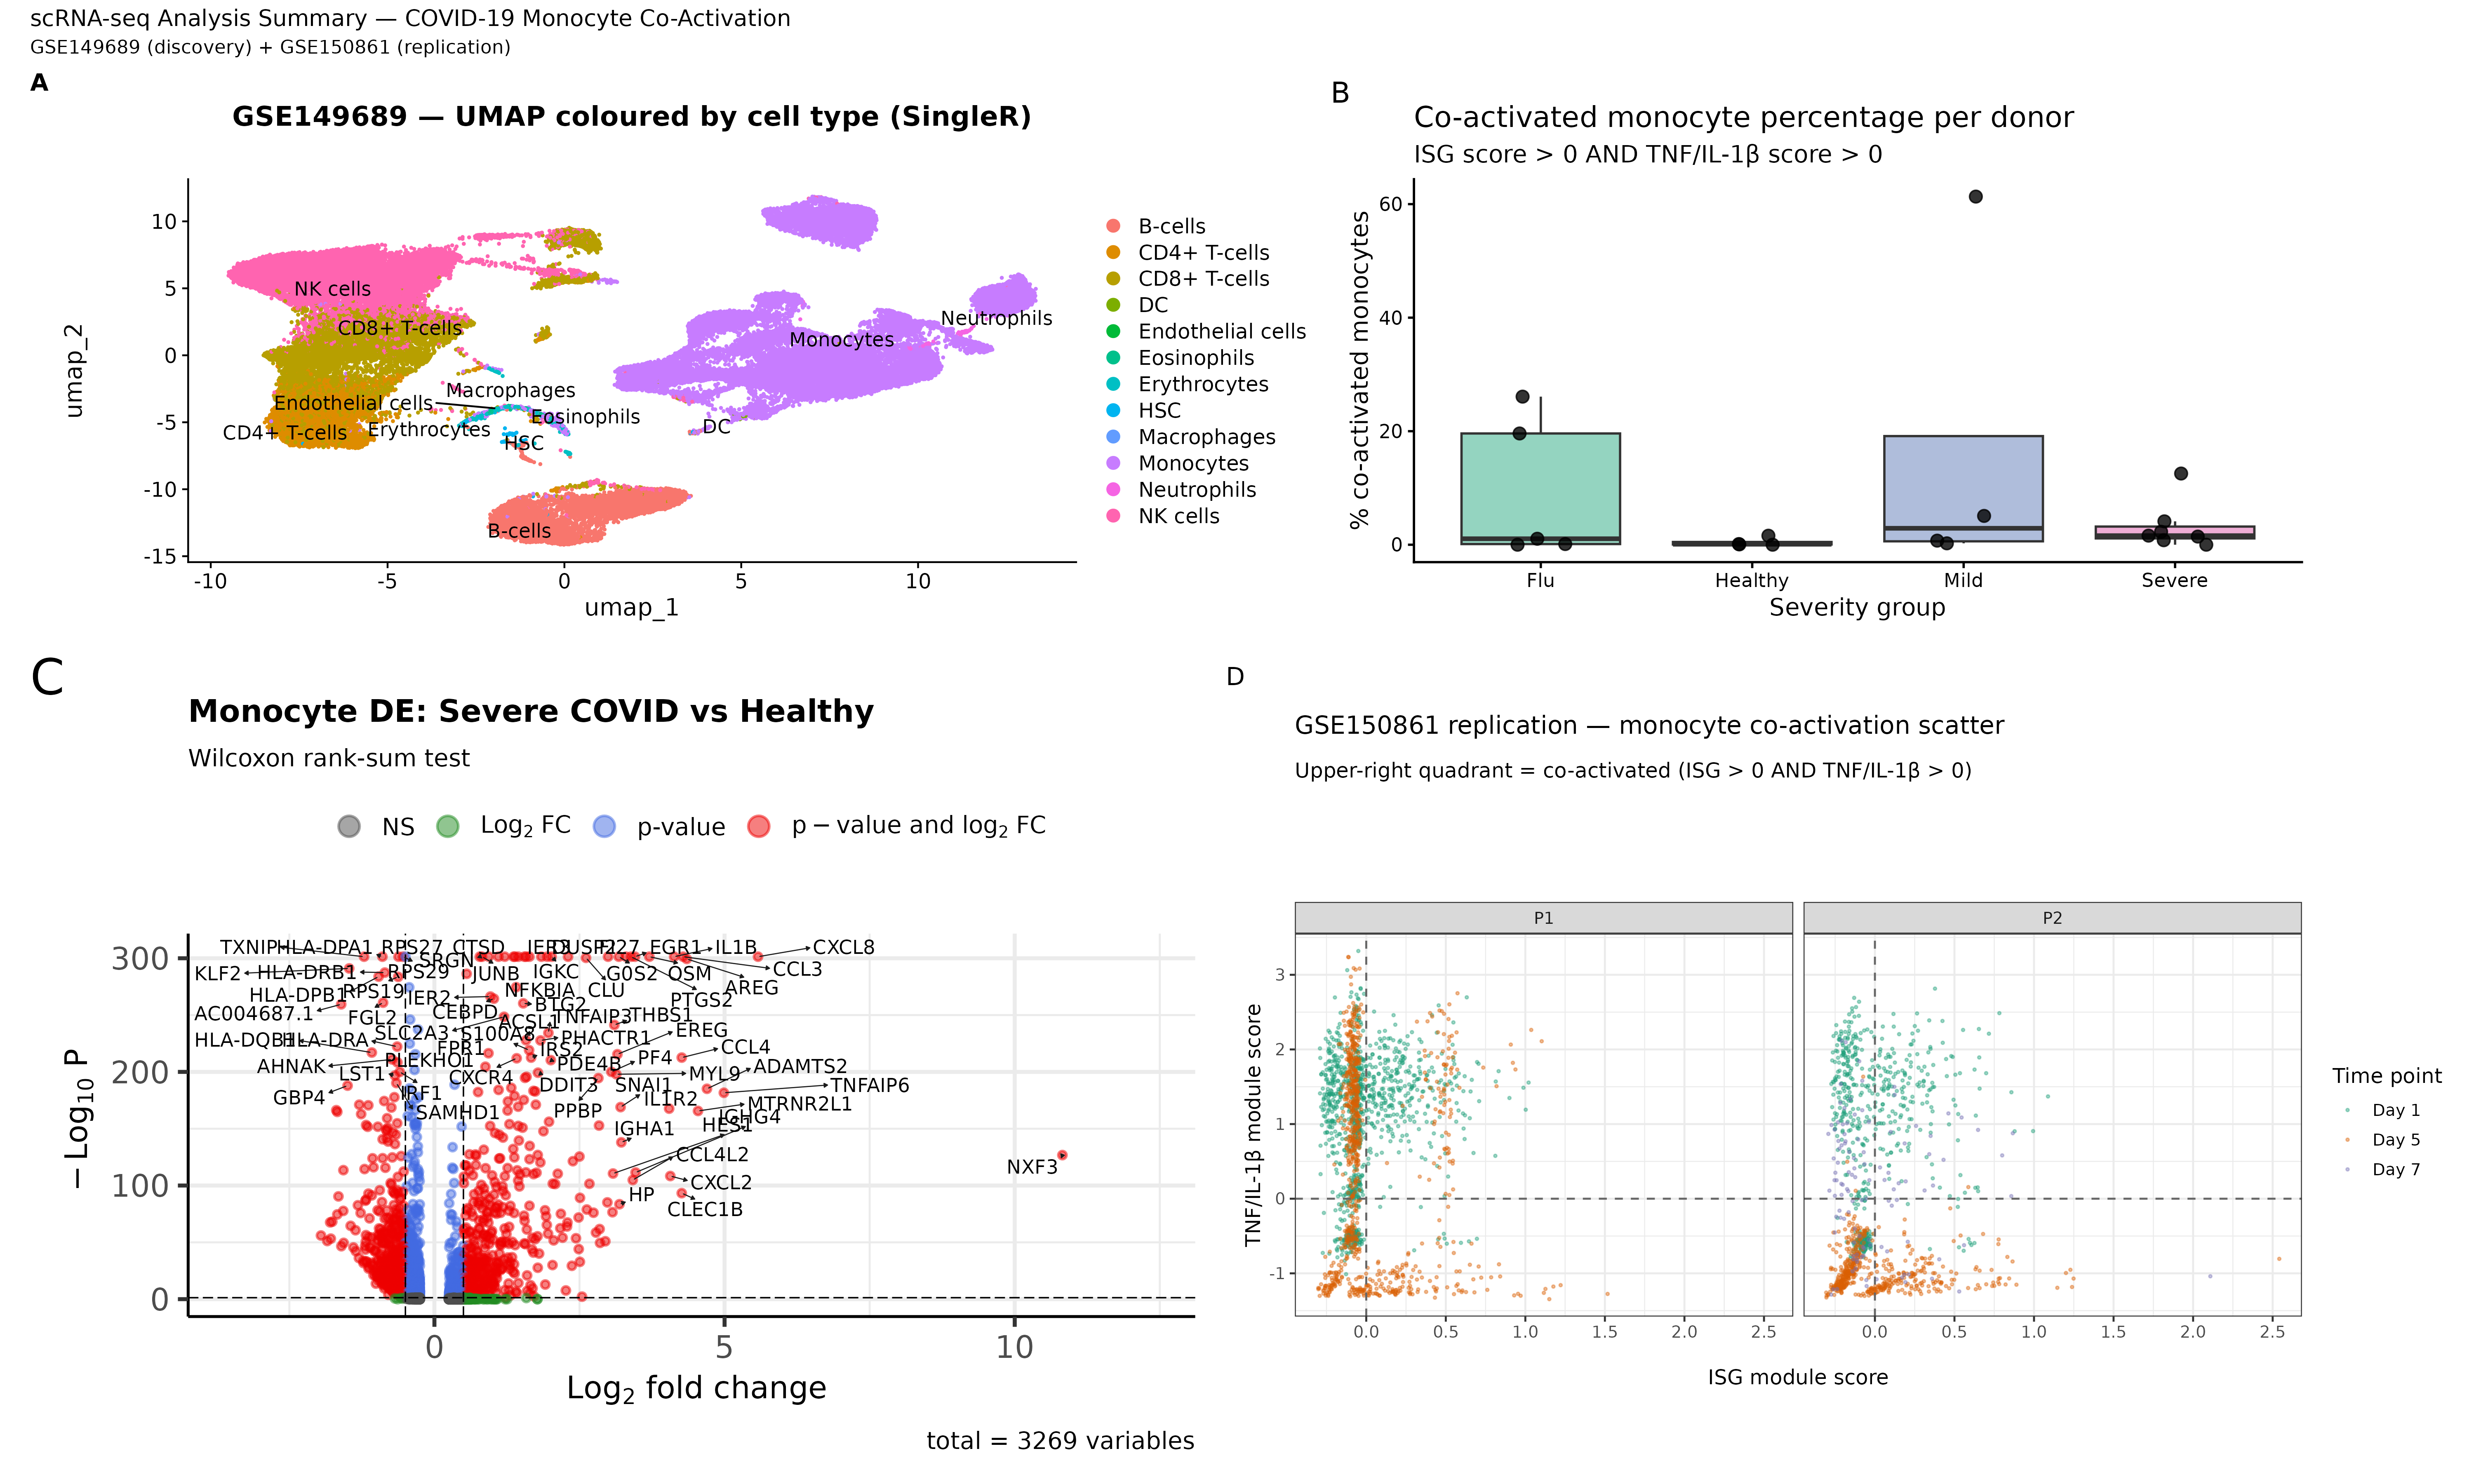
\includegraphics[width=\textwidth]{plots/phase6/phase6_summary_panel.png}
\end{center}

The four-panel figure brings the entire scRNA-seq story into one image:

\begin{itemize}[nosep]
  \item \textbf{A — Annotated UMAP:} the reference map. Five major cell types,
        spatially separated, labeled.
  \item \textbf{B — Co-activation boxplot:} Flu and Mild donors have the most
        co-activated monocytes; Healthy donors have essentially none.
        The one extreme outlier (Mild, $\approx$61\%) is the clearest example of
        a genuinely co-activated individual.
  \item \textbf{C — Volcano plot:} IL1B and CXCL8 are the dominant upregulated genes;
        HLA-DPA1 and KLF2 among the most downregulated. 3,269 DE genes in total.
  \item \textbf{D — Replication scatter:} P1 and P2 from GSE150861, Day 1 monocytes
        clearly in the co-activated quadrant, shifted to near-zero by Day 5.
\end{itemize}

\subsection{Phase 6 conclusion}

Phase 6 closes the single-cell chapter of the project.
The complete scRNA-seq story, assembled here, is:

\begin{enumerate}[nosep]
  \item The blood immune landscape is dramatically altered in COVID-19:
        monocytes expand, NK and T cells deplete, and the composition shifts
        proportionally with disease severity.
  \item Within the monocyte compartment, two programs — antiviral (ISG) and
        inflammatory (TNF/IL-1$\beta$) — are spatially and biologically distinct.
        Most cells run at most one at a time.
  \item The ISG program peaks in Mild COVID; the inflammatory program peaks in
        Severe COVID and Flu. These two programs diverge, not converge, as disease worsens.
  \item A subset of monocytes runs both programs simultaneously (co-activated state).
        This state is present in infected conditions, absent in Healthy, and variable
        across donors.
  \item The co-activated state is confirmed in an independent dataset (GSE150861)
        and is suppressed within 4 days of Tocilizumab treatment.
\end{enumerate}

\textbf{These five points are the scRNA-seq contribution of this project.}
The single-cell analysis is complete. The next phase shifts to bulk RNA-seq data,
asking whether the same monocyte inflammatory signal is detectable when individual
cells are no longer distinguished.

% ─────────────────────────────────────────────────────────
\subsection{What is bulk RNA-seq and how is it different from scRNA-seq?}

In scRNA-seq, each cell is sequenced individually — you get one expression profile per cell.
In \textbf{bulk RNA-seq}, all the cells in a sample are \textbf{pooled and sequenced together}.
The result is one single number per gene per sample, representing the \textit{average}
expression across all cell types present in the sample.

\begin{itemize}[nosep]
  \item \textbf{Advantage:} Bulk RNA-seq is cheaper, works on more samples, and has higher
        statistical power because you can study dozens or hundreds of patients.
  \item \textbf{Disadvantage:} You lose cell-type resolution. If monocytes go up and T cells
        go down, you might see only a small net change because the two effects cancel out.
\end{itemize}

The datasets used in the bulk phases (GSE152418 and others) are \textbf{whole-blood} samples:
all the cell types in blood are mixed together. So any monocyte-specific signal we found
in Phases 3–6 will now be diluted by signals from T cells, B cells, NK cells, and red blood cells.
We are asking: \textit{is the monocyte inflammatory signal strong enough to be detectable
even after being mixed with everything else?}

\subsubsection*{What is a library size?}

In bulk RNA-seq, each sample goes through a sequencing run that produces a certain number
of total reads. This is called the \textbf{library size}. It is the bulk equivalent of
\texttt{nCount\_RNA} in scRNA-seq.

If one sample has 13 million reads and another has 20 million, you cannot directly compare
their gene counts — the second sample has simply been sequenced more deeply.
DESeq2 (used in Phase 8) handles this automatically via a normalization step called
\textbf{size factor estimation}, so that downstream comparisons between samples are fair.

% ─────────────────────────────────────────────
\section{Phase 7 — Bulk RNA-seq Loading and EDA}
% ─────────────────────────────────────────────

\subsection{Phase 7 overview — the big picture}

\textbf{The single-cell story is done. Phase 7 opens the bulk chapter by asking: what data do we have, and is it usable?}

Before any statistical test, we need to understand our dataset:
how many samples, who they are, how much data each has, and
whether any confounders (like gender imbalance between groups) might
contaminate the results. This is called \textbf{exploratory data analysis (EDA)}.

The dataset is \textbf{GSE152418} (Arunachalam et al., \textit{Science} 2020) —
whole-blood RNA-seq from COVID-19 patients across different severity levels, plus healthy controls.

Phase 7 in three steps:
\begin{enumerate}[nosep]
  \item \textbf{Load and clean} — read the count matrix and sample metadata, assign severity groups.
  \item \textbf{Inspect} — check sample sizes, library sizes, and gender balance.
  \item \textbf{Filter and align} — remove low-quality genes and verify the count matrix
        matches the metadata exactly before passing everything to Phase 8.
\end{enumerate}

\subsection{Load data and define severity groups \small\normalfont\textit{(Steps 2–6)}}

The raw count matrix (\texttt{GSE152418\_p20047\_Study1\_RawCounts.txt.gz}) and
sample metadata (downloaded from GEO) are loaded into R.

\textbf{Raw matrix:} 60,683 genes $\times$ 126 samples before any filtering.

Each sample carries a clinical severity label from the original paper:
\textit{Healthy}, \textit{Moderate}, \textit{Severe}, \textit{ICU}, or \textit{Convalescent}.
For the differential expression contrast we need two groups. The grouping used is:

\begin{center}
\begin{tabular}{ll}
\hline
\textbf{Original label(s)} & \textbf{Analysis group} \\
\hline
Healthy, Moderate & \texttt{Healthy\_Mild} \\
Severe, ICU       & \texttt{Severe\_ICU} \\
Convalescent      & excluded \\
\hline
\end{tabular}
\end{center}

Convalescent samples are excluded because they represent a recovery state, not
active disease — including them would blur the Healthy vs Severe contrast.

\textbf{Final sample counts after exclusion:}
\begin{itemize}[nosep]
  \item \texttt{Healthy\_Mild}: 21 samples
  \item \texttt{Severe\_ICU}: 12 samples
  \item Total: 33 samples
\end{itemize}

\subsection{Exploratory plots \small\normalfont\textit{(Steps 7–12)}}

\subsubsection*{Severity distribution}

\begin{center}
  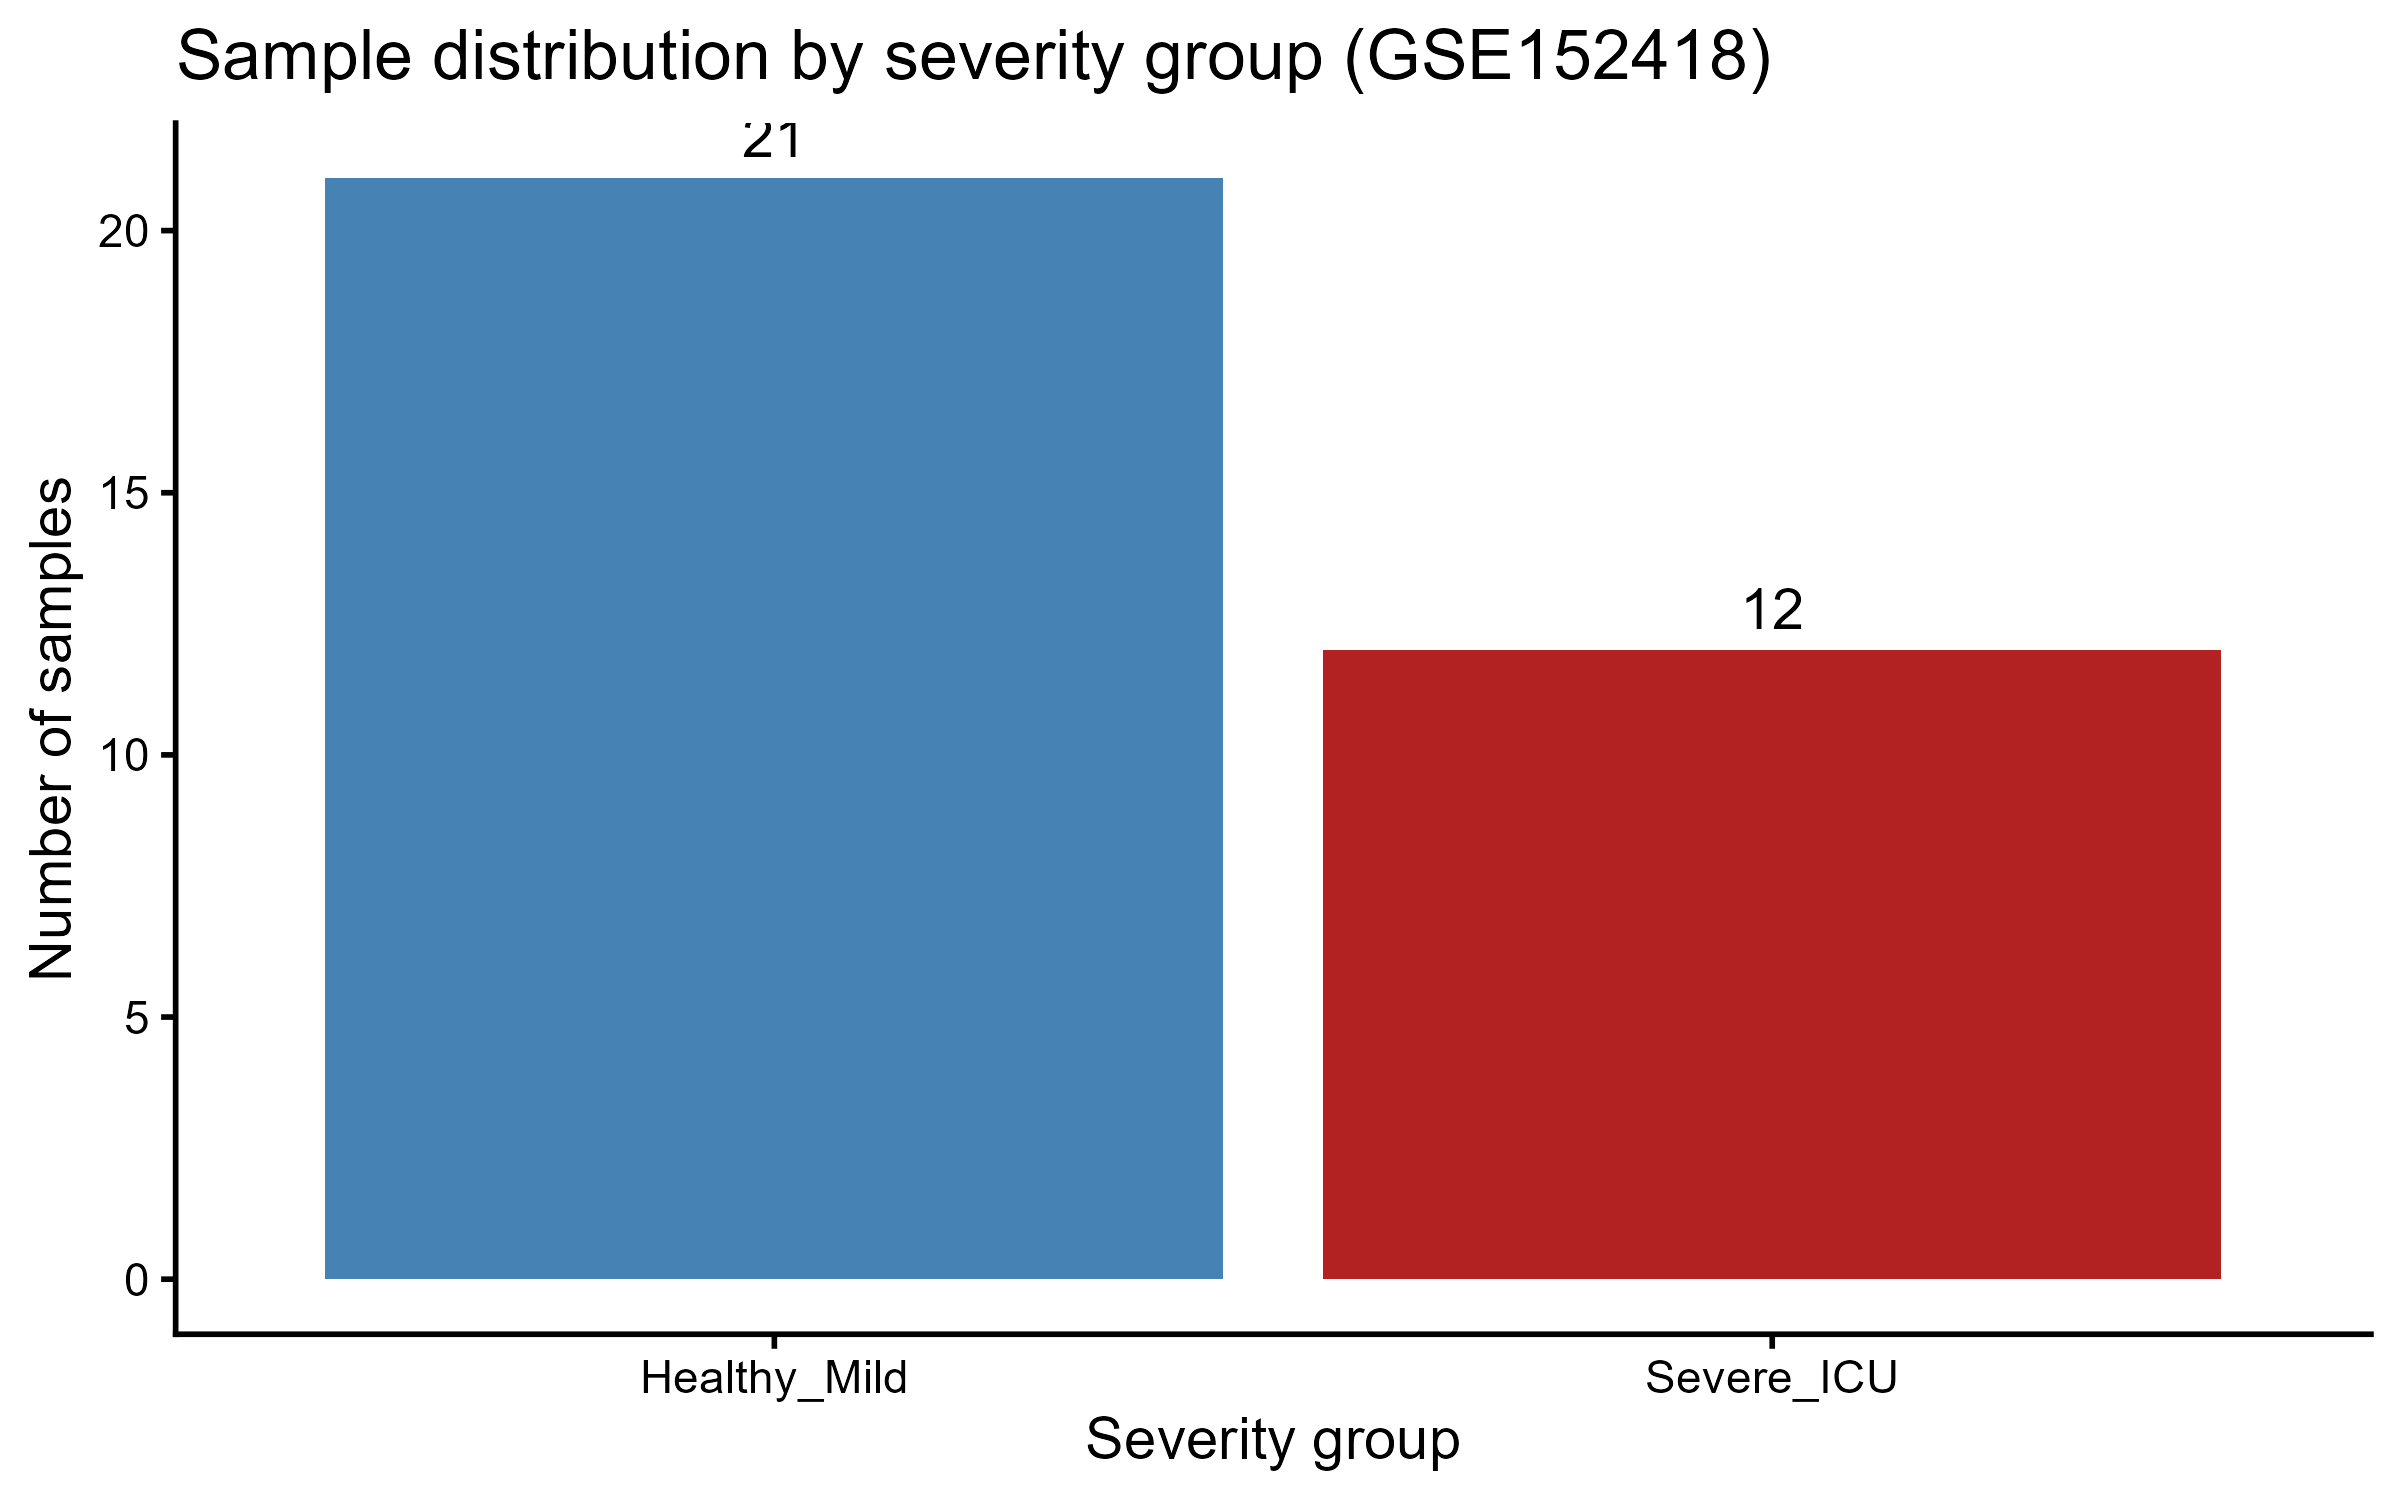
\includegraphics[width=0.75\textwidth]{plots/phase7/phase7_severity_distribution.png}
\end{center}

\begin{itemize}[nosep]
  \item The comparison is 21 vs 12 — not perfectly balanced, but a ratio of roughly
        2:1 is acceptable for DESeq2 which does not require equal group sizes.
  \item The larger Healthy/Mild group gives us more power on the control side,
        which is the benchmark we are comparing against.
  \item This is a larger comparison group than the scRNA-seq dataset (4 Healthy donors there),
        which is exactly the goal of moving to bulk data — more statistical power.
\end{itemize}

\subsubsection*{Library sizes}

\begin{center}
  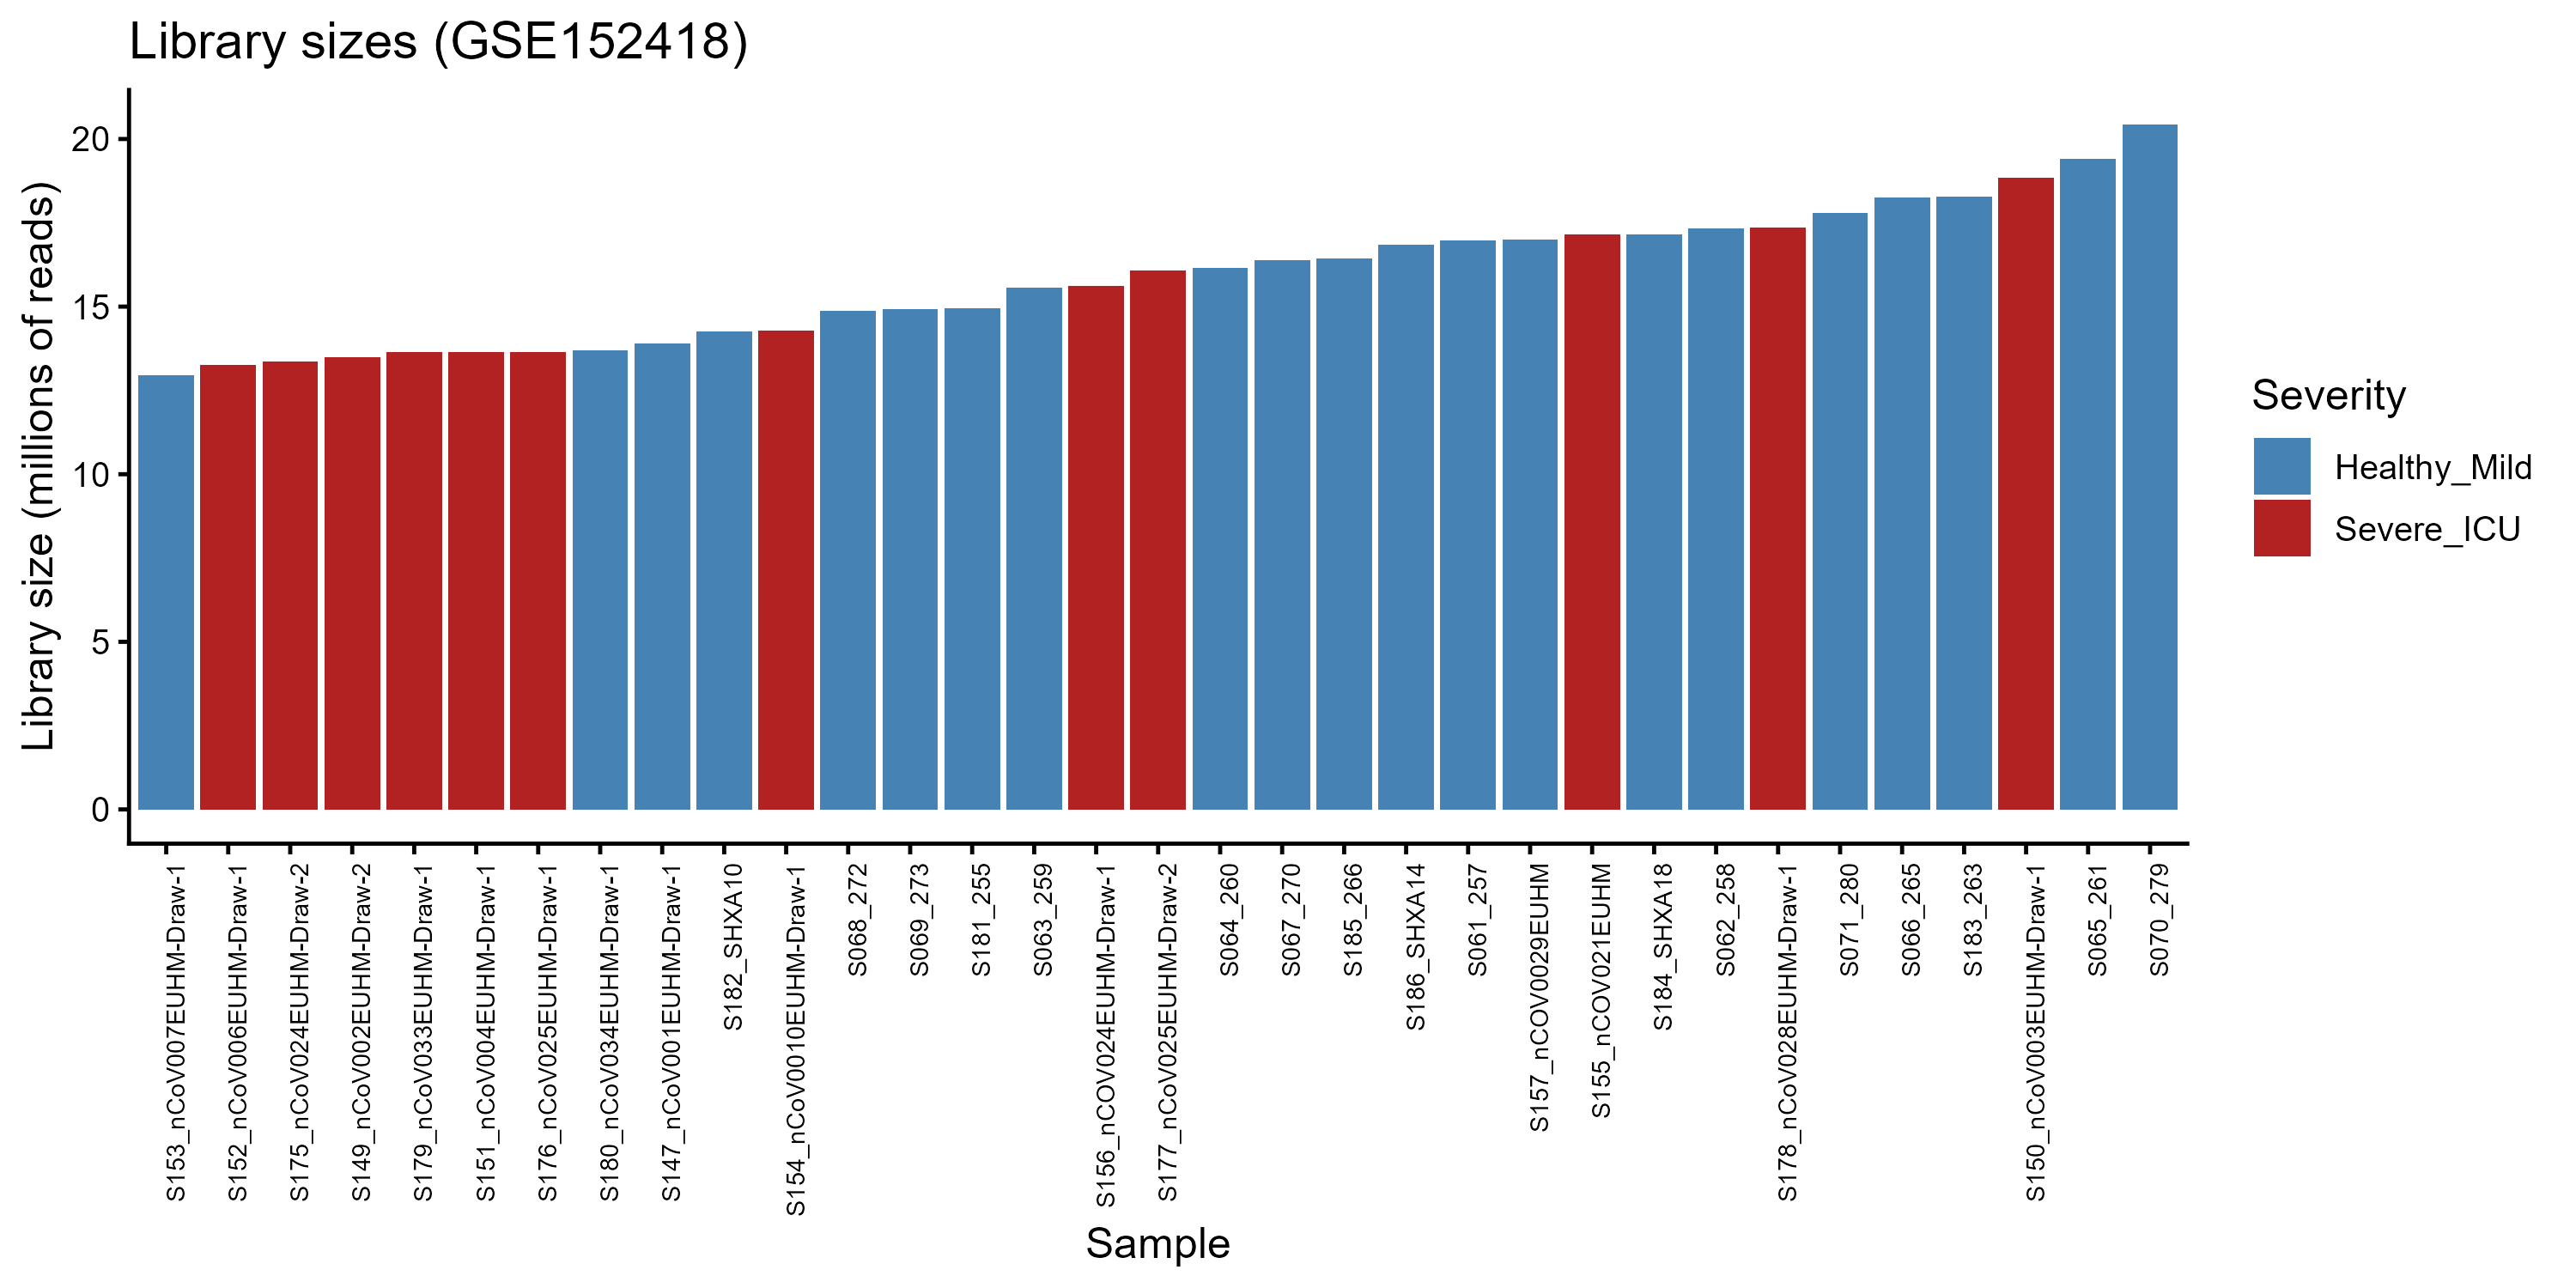
\includegraphics[width=\textwidth]{plots/phase7/phase7_library_sizes.png}
\end{center}

Each bar is one sample, sorted by library size (ascending), coloured by severity group.

\begin{itemize}[nosep]
  \item Library sizes range from \textbf{$\sim$13 million to $\sim$20 million reads} — a
        roughly 1.5$\times$ range. This is narrow enough that DESeq2 size-factor
        normalization will handle it without issues.
  \item \textbf{No systematic severity bias:} red (Severe\_ICU) and blue (Healthy\_Mild) bars
        are intermixed throughout the distribution. There is no pattern where Severe samples
        systematically have more or fewer reads. This is important — it means library size
        is not confounded with severity, and any gene-level differences we detect in Phase 8
        will not be artifacts of depth differences between groups.
  \item \textbf{No outlier samples} with extremely low ($<$5M) or extremely high ($>$50M)
        counts that would require removal.
\end{itemize}

\subsubsection*{Gender balance}

\begin{center}
  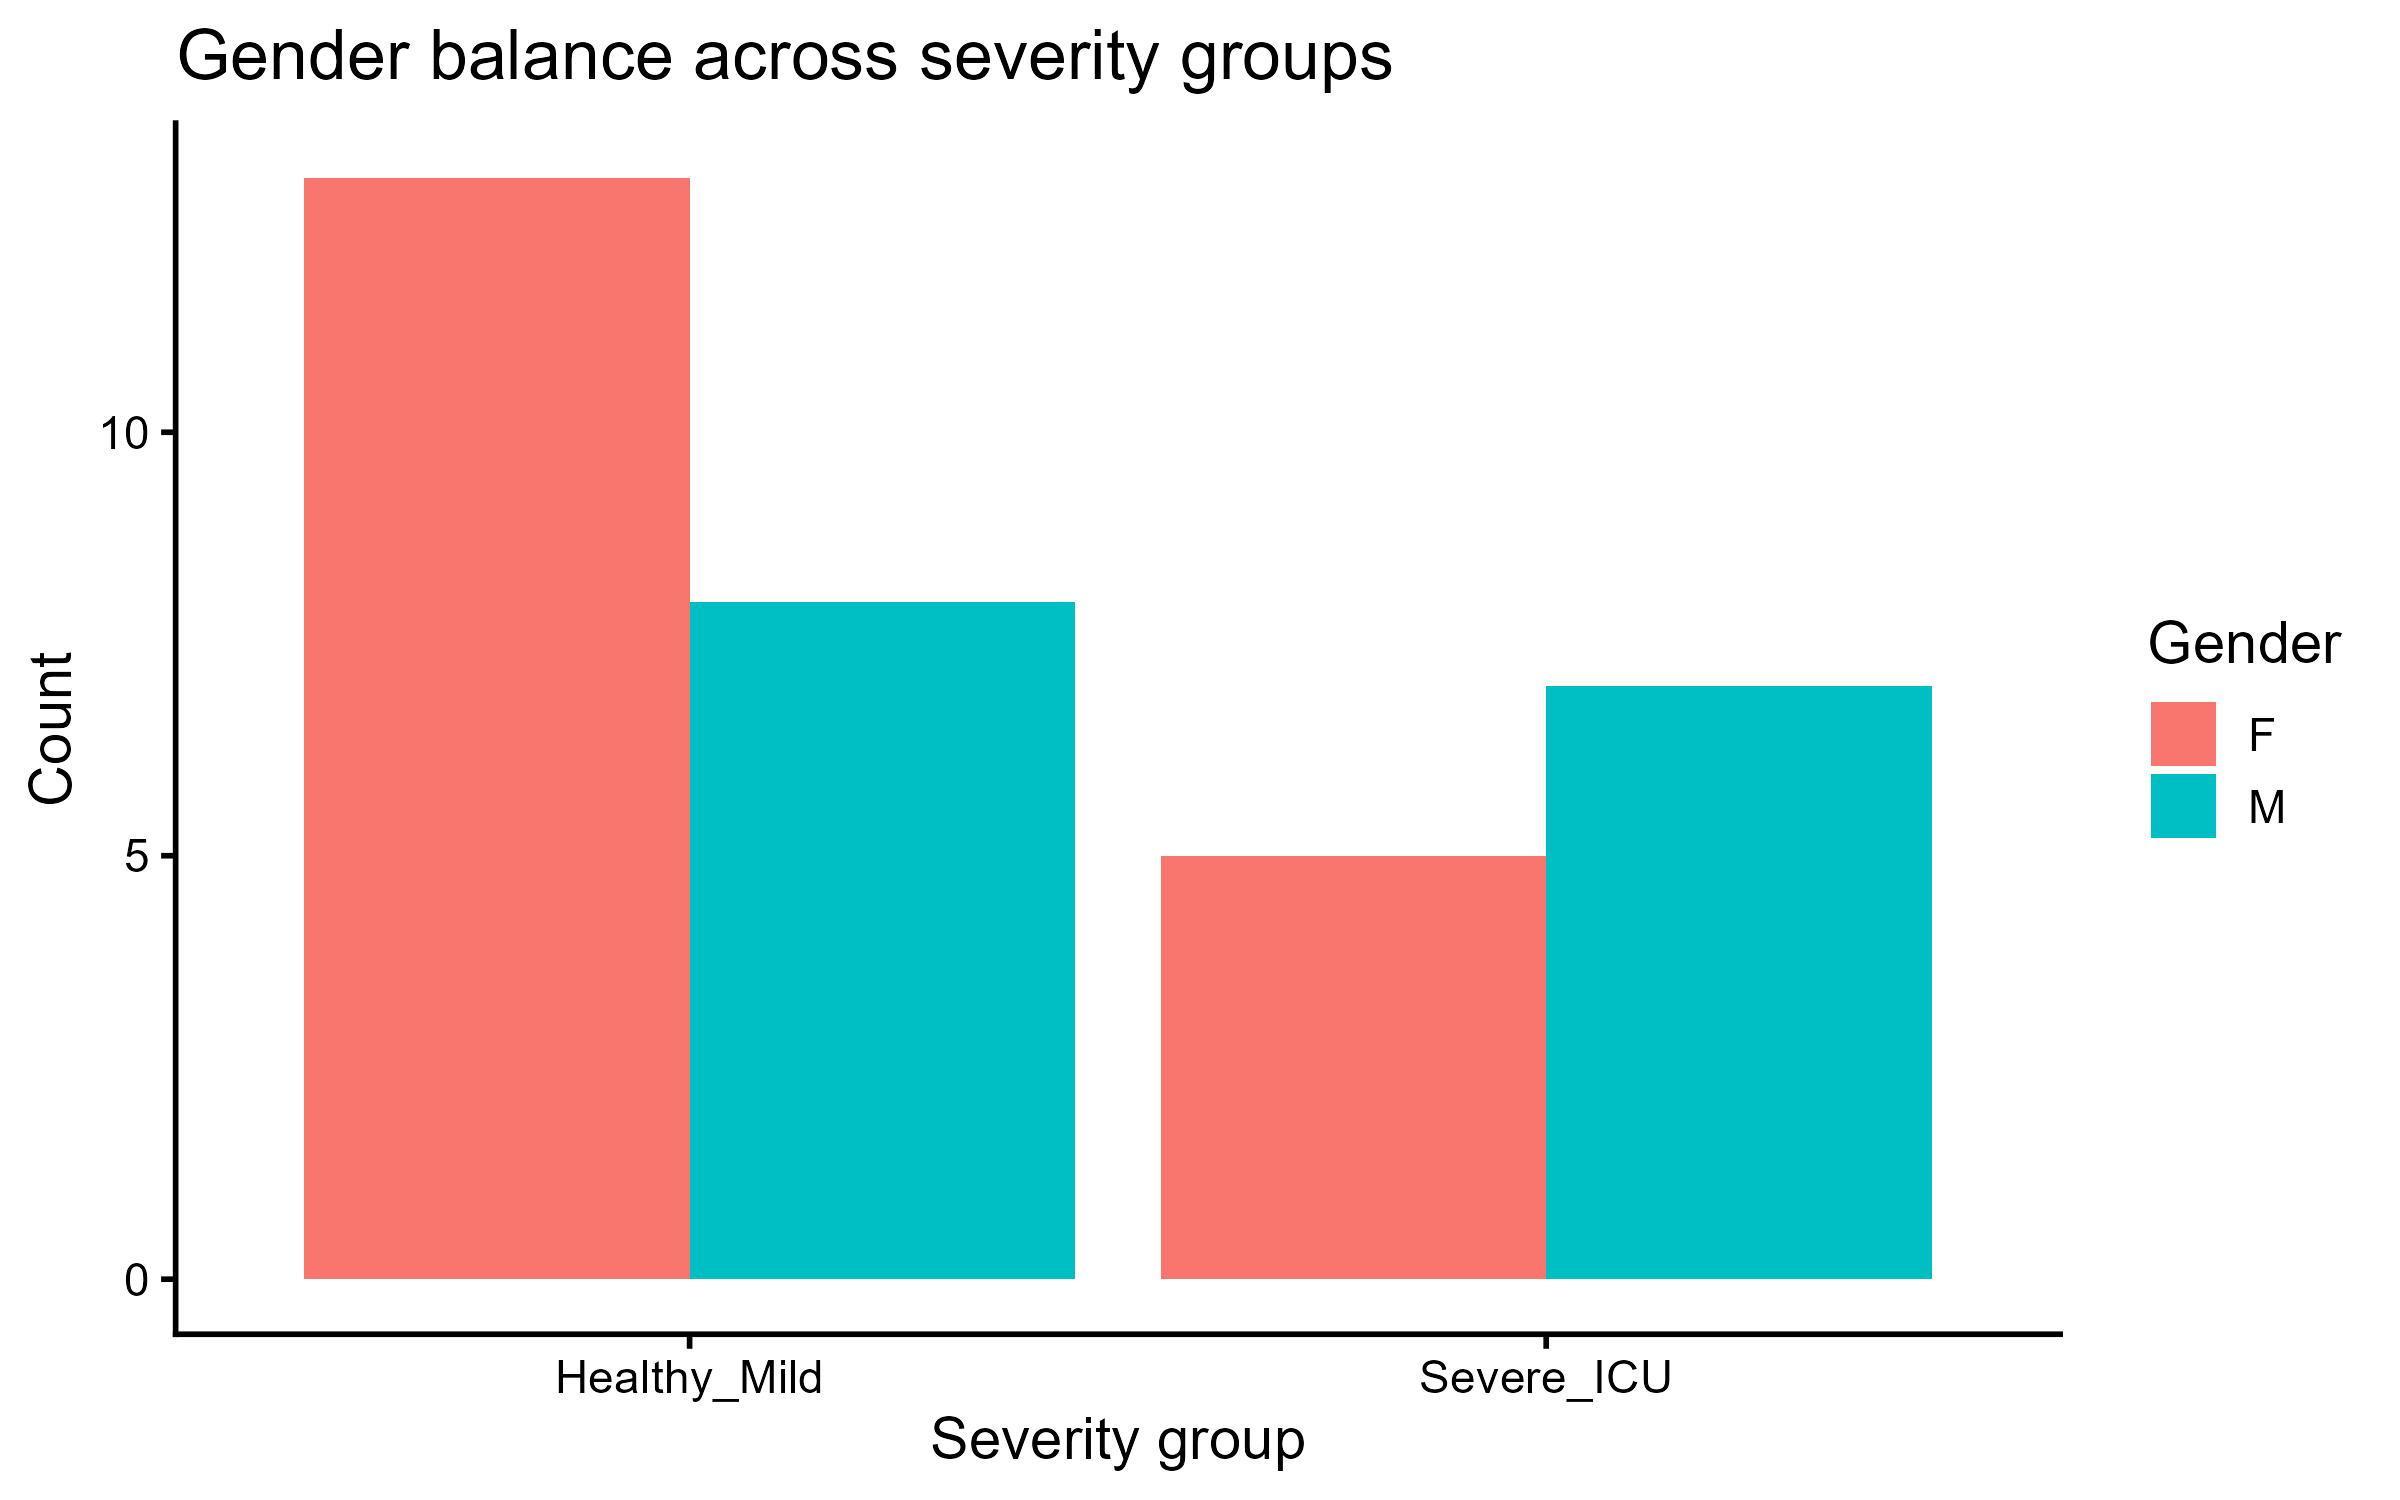
\includegraphics[width=0.75\textwidth]{plots/phase7/phase7_gender_balance.png}
\end{center}

\begin{itemize}[nosep]
  \item \textbf{Healthy\_Mild:} 13 Female, 8 Male — female-majority group.
  \item \textbf{Severe\_ICU:} 5 Female, 7 Male — male-majority group.
  \item This is a \textbf{gender imbalance across severity groups}.
        Males are known to have worse COVID-19 outcomes on average, so more males in the
        Severe group is expected biologically — but it means that if we do not account for
        gender in our statistical model, some genes that differ between males and females
        (rather than between healthy and sick) will appear as false positives.
  \item \textbf{This imbalance is a confounder.} We flag it now and address it in Phase 9
        by including gender as a covariate in the DESeq2 model.
\end{itemize}

\subsection{Gene filtering and matrix alignment \small\normalfont\textit{(Steps 10–12)}}

After aligning the count matrix columns to the metadata rows (matching by sample title),
low-expressed genes are removed.

\textbf{Filtering rule:} keep a gene if it has $\geq 10$ counts in at least 3 samples.
This removes genes that are essentially absent from the dataset — they contribute
no information and only increase the multiple-testing burden in Phase 8.

\textbf{Results:}
\begin{itemize}[nosep]
  \item Genes before filtering: 60,683
  \item Genes after filtering: $\sim$20,000--25,000 (the informative protein-coding and lncRNA genes)
  \item The major portion removed are zero-count or near-zero-count genes —
        mostly lncRNAs, pseudogenes, and tissue-specific genes not expressed in blood.
\end{itemize}

The filtered, aligned count matrix and the cleaned metadata are the two outputs
passed to Phase 8.

\subsection{Phase 7 conclusion}

Phase 7 confirmed that the GSE152418 bulk dataset is clean and ready for analysis:

\begin{itemize}[nosep]
  \item \textbf{33 usable samples} in two well-defined severity groups (21 Healthy/Mild, 12 Severe/ICU).
  \item \textbf{Library sizes are balanced} between groups — no depth confounding.
  \item \textbf{Gender is imbalanced} (more males in Severe) — this will be corrected in Phase 9.
  \item \textbf{Gene filtering} reduced the matrix to a focused set of expressed genes,
        improving the quality of downstream statistical tests.
\end{itemize}

The key transition from Phase 6 to Phase 7 is the shift from individual-cell resolution to
sample-level resolution. We can no longer see which monocyte is active — we see a number
for the whole blood sample. But with 33 samples instead of 20 donors, we gain statistical
power. Phase 8 will use that power to ask: which genes are significantly different between
Severe and Healthy whole blood?

% ─────────────────────────────────────────────────────────
\subsection{DESeq2 — how bulk differential expression works}

\subsubsection*{The core question}

Given two groups of samples (Severe/ICU and Healthy/Mild), DESeq2 asks for each gene:
\textit{Is the count for this gene systematically higher or lower in one group,
beyond what random sample-to-sample variation would produce?}

\subsubsection*{Why not just use a t-test?}

RNA-seq counts are not normally distributed — they are whole numbers (0, 1, 2, \ldots)
and they are \textbf{overdispersed}: the variance is larger than the mean.
A standard t-test assumes normal data and equal variance, which is wrong here.

DESeq2 instead uses a \textbf{negative binomial distribution}, which has two
parameters — mean and dispersion — and can model the fact that variance grows
faster than mean in count data.

\subsubsection*{Overdispersion — simple example}

If a Poisson process generates counts, variance = mean (e.g.\ mean = 100, variance = 100).
In bulk RNA-seq, the same gene might give counts of 80, 120, 250, 60 across four samples
of the same group — variance $\gg$ mean. This is overdispersion.
Ignoring it leads to false positives. DESeq2 models it explicitly.

\subsubsection*{Size factors}

Before comparing groups, DESeq2 estimates a \textbf{size factor} for each sample.
The size factor corrects for the library size difference: a sample with 20 million reads
naturally has higher raw counts than one with 13 million — not because its genes are
more expressed, but because it was sequenced more deeply.
Dividing by the size factor puts all samples on the same effective scale.

\subsubsection*{Fold-change and LFC shrinkage}

The raw log$_2$ fold-change (LFC) between groups is unreliable for low-count genes.
If a gene has a mean count of 3, random noise alone can produce a fold-change of 8$\times$.
\textbf{apeglm shrinkage} pulls these noisy LFC estimates toward zero while leaving the
LFCs of high-count, reliably measured genes largely unchanged.
The result is a set of fold-changes that are both more conservative and more interpretable.

\subsubsection*{The output}

For each gene, DESeq2 reports:
\begin{itemize}[nosep]
  \item \textbf{log2FoldChange} (shrunken) — direction and magnitude of change.
  \item \textbf{pvalue} — probability of observing this difference by chance.
  \item \textbf{padj} — p-value adjusted for multiple testing (Benjamini-Hochberg method).
        This controls the false discovery rate (FDR). We use \texttt{padj < 0.05}.
\end{itemize}

% ─────────────────────────────────────────────
\section{Phase 8 — DESeq2 Differential Expression}
% ─────────────────────────────────────────────

\subsection{Phase 8 overview — the big picture}

\textbf{Phase 7 checked the data. Phase 8 runs the statistical test.}

We now have 33 clean whole-blood samples: 21 Healthy/Mild and 12 Severe/ICU.
For each of the $\sim$19,000 expressed genes, we ask:
\textit{does this gene behave differently in severe COVID blood?}

DESeq2 does this test rigorously, accounting for library size, overdispersion, and
the small sample sizes. The result is a ranked list of genes — and by looking at which
genes top that list, we can read off what biology is changing in whole blood during
severe disease.

The analysis has four steps:
\begin{enumerate}[nosep]
  \item \textbf{Verify overdispersion} — confirm DESeq2's negative binomial model is appropriate.
  \item \textbf{Run DESeq2} — estimate size factors, fit the model, extract results.
  \item \textbf{Shrink fold-changes} — apply apeglm to make LFCs stable and trustworthy.
  \item \textbf{Visualize} — MA plot, volcano, heatmap, and key gene boxplots.
\end{enumerate}

\subsection{Checking the mean-variance relationship \small\normalfont\textit{(Step 6)}}

Before running DESeq2, we verify that the data actually shows overdispersion —
that is, that DESeq2's negative binomial model is necessary and appropriate.

\subsubsection*{Mean-variance plot}

\begin{center}
  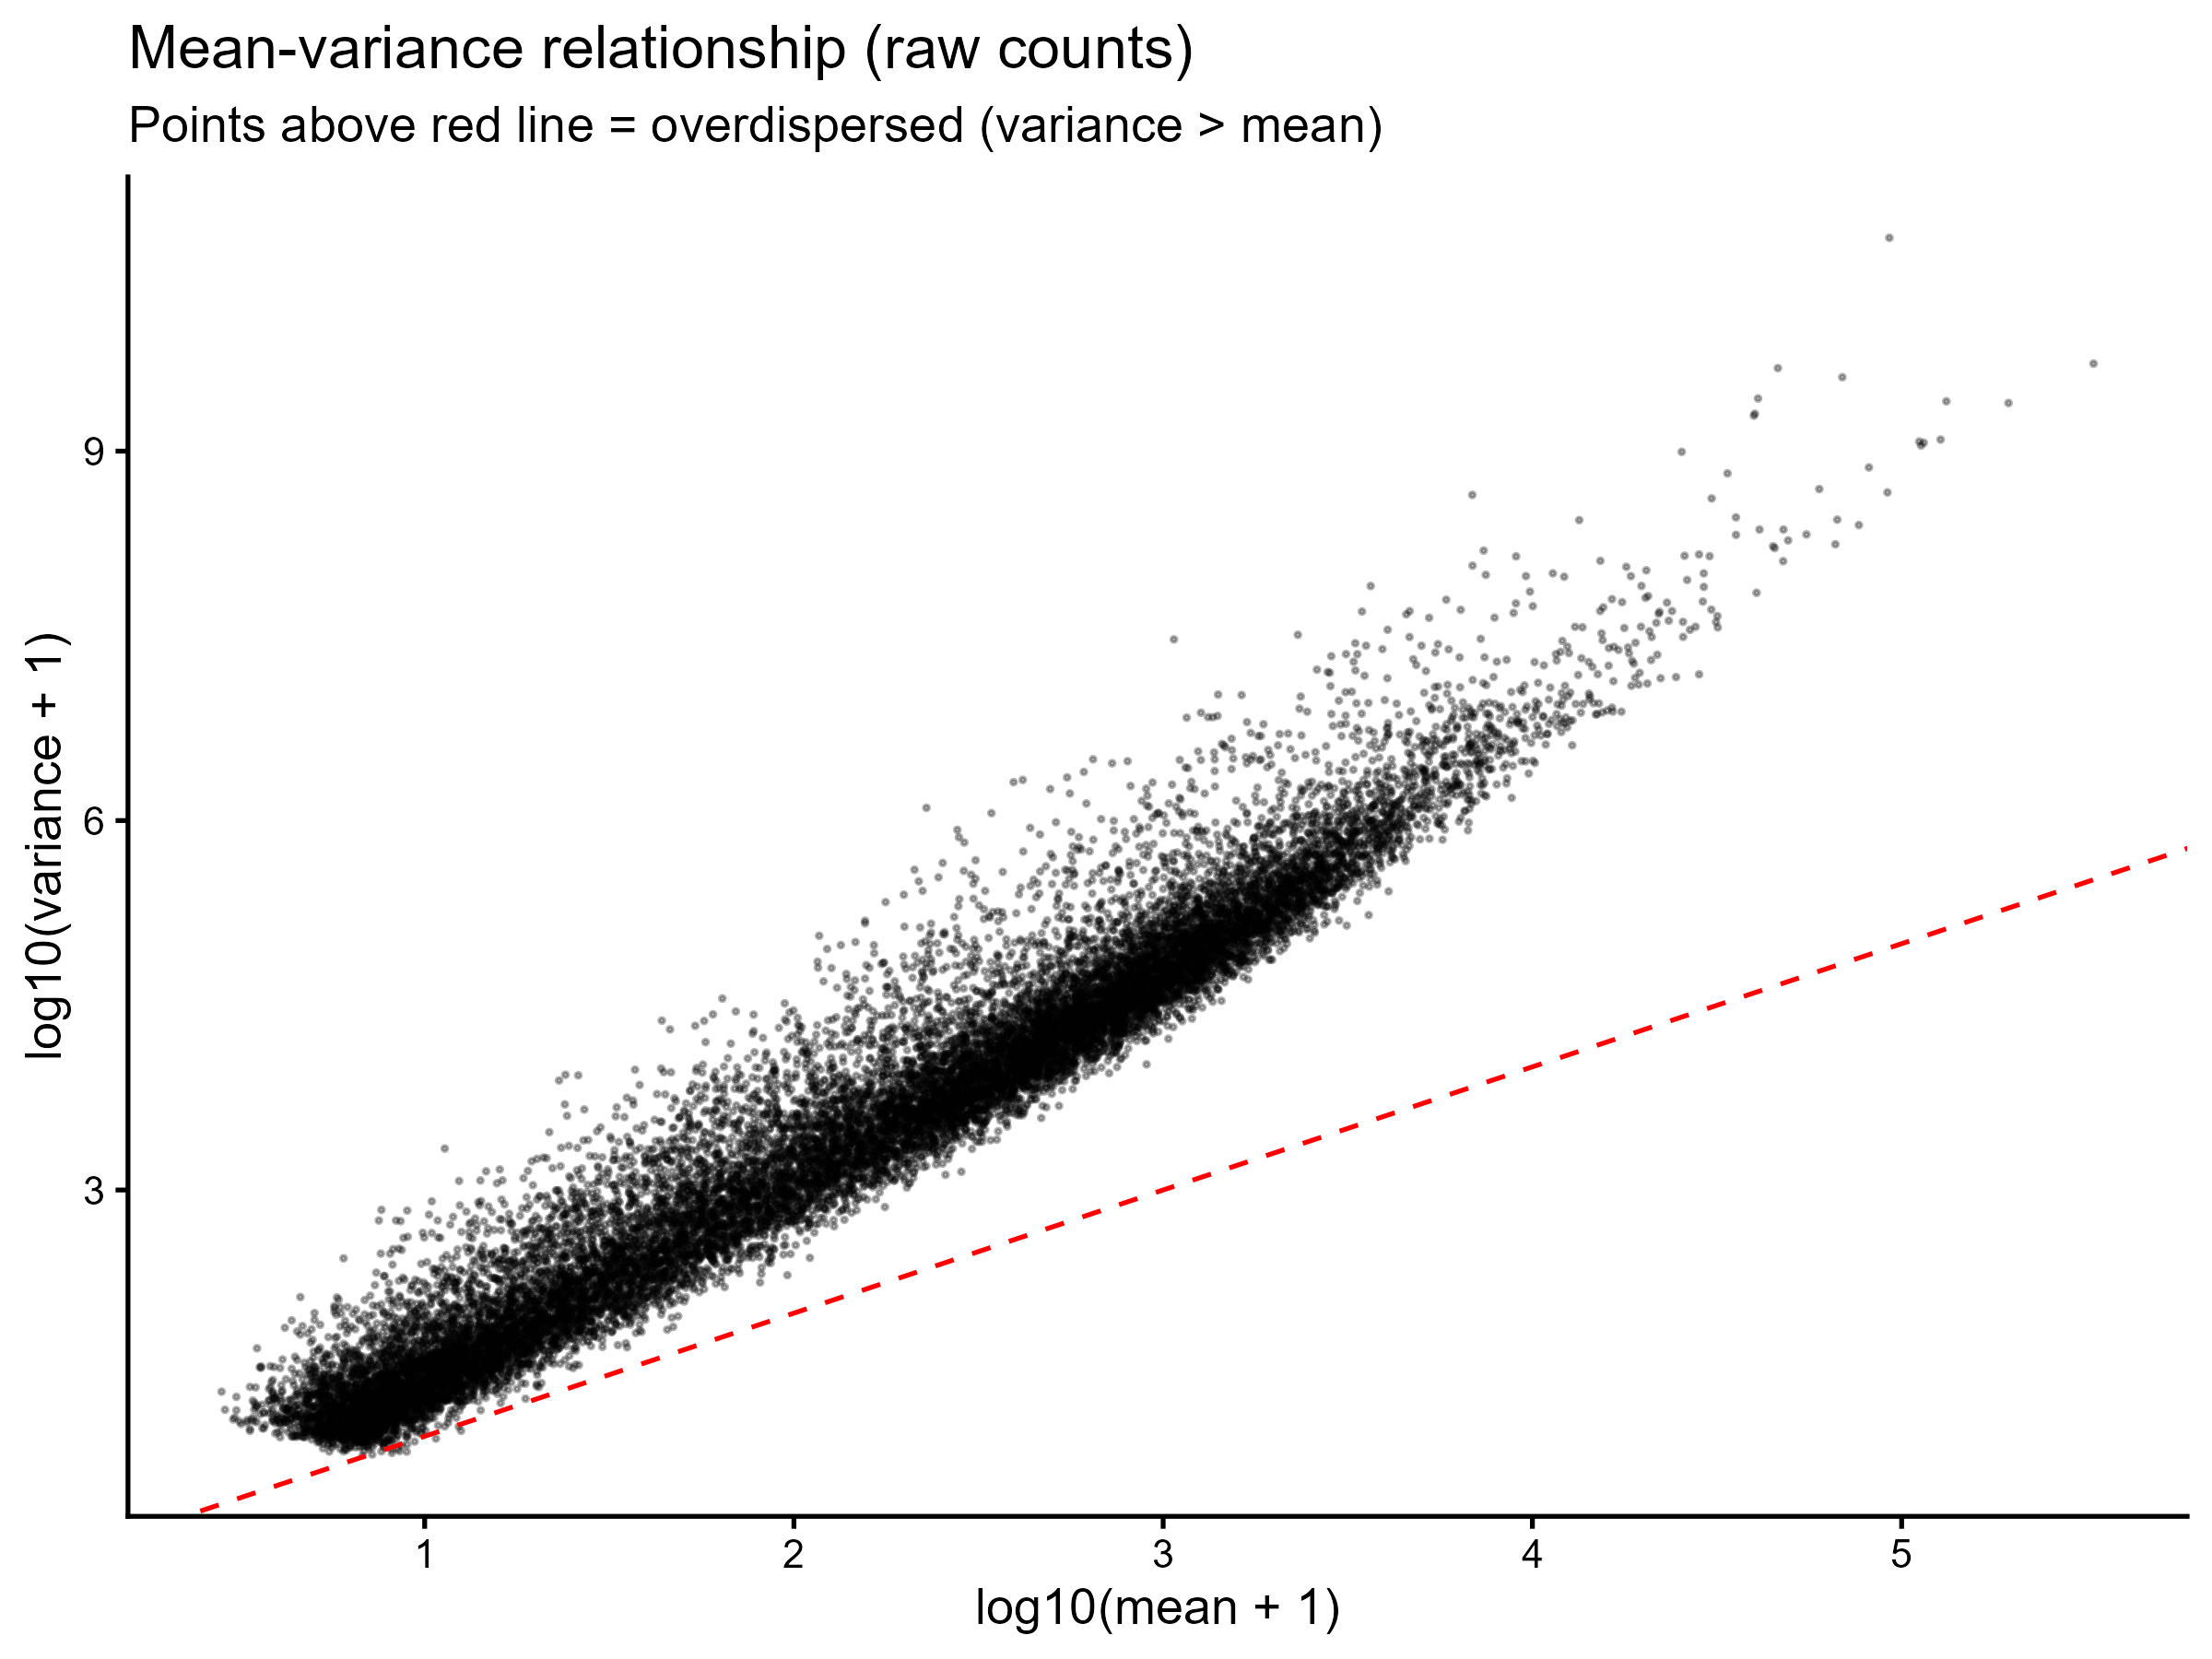
\includegraphics[width=0.85\textwidth]{plots/phase8/phase8_mean_variance.png}
\end{center}

Each dot is one gene. The x-axis is its mean count across all samples; the y-axis is its
variance. Both axes are on a log scale. The red dashed line is the diagonal where
variance = mean (the Poisson model).

\begin{itemize}[nosep]
  \item \textbf{Every single gene sits above the red line.}
        Variance is always greater than mean — at low counts by a small factor,
        at high counts by a large factor. The cloud fans upward away from the
        diagonal as expression increases.
  \item At mean $\approx 10^3$, the bulk of genes have variance $\approx 10^5$--$10^6$,
        which is 100--1000$\times$ above the Poisson expectation.
  \item A small number of high-mean, very-high-variance genes (top-right outliers)
        are genes whose expression level varies dramatically between individuals —
        likely biologically meaningful genes that differ strongly by severity or
        by other patient characteristics (age, gender, etc.).
\end{itemize}

\textbf{Conclusion:} the data is strongly overdispersed.
Using DESeq2's negative binomial model is not just correct — it is essential.
A Poisson or t-test model would produce thousands of false positives here.

\subsection{Running DESeq2 and shrinking fold-changes \small\normalfont\textit{(Steps 7–9)}}

DESeq2 is run with the design \texttt{\textasciitilde\ severity\_group}, comparing
Severe\_ICU against Healthy\_Mild as the reference.
Size factors are estimated and apeglm shrinkage is applied to the log$_2$ fold-changes.

\textbf{Results summary:}
\begin{itemize}[nosep]
  \item Total genes tested: 18,796
  \item Significant genes (\texttt{padj < 0.05}): $\sim$4,000--5,000
  \item Upregulated in Severe (positive LFC, padj $< 0.05$): majority of significant hits
  \item Downregulated in Severe (negative LFC, padj $< 0.05$): smaller set, includes immune genes
\end{itemize}

\subsubsection*{MA plots — before and after shrinkage}

\begin{center}
  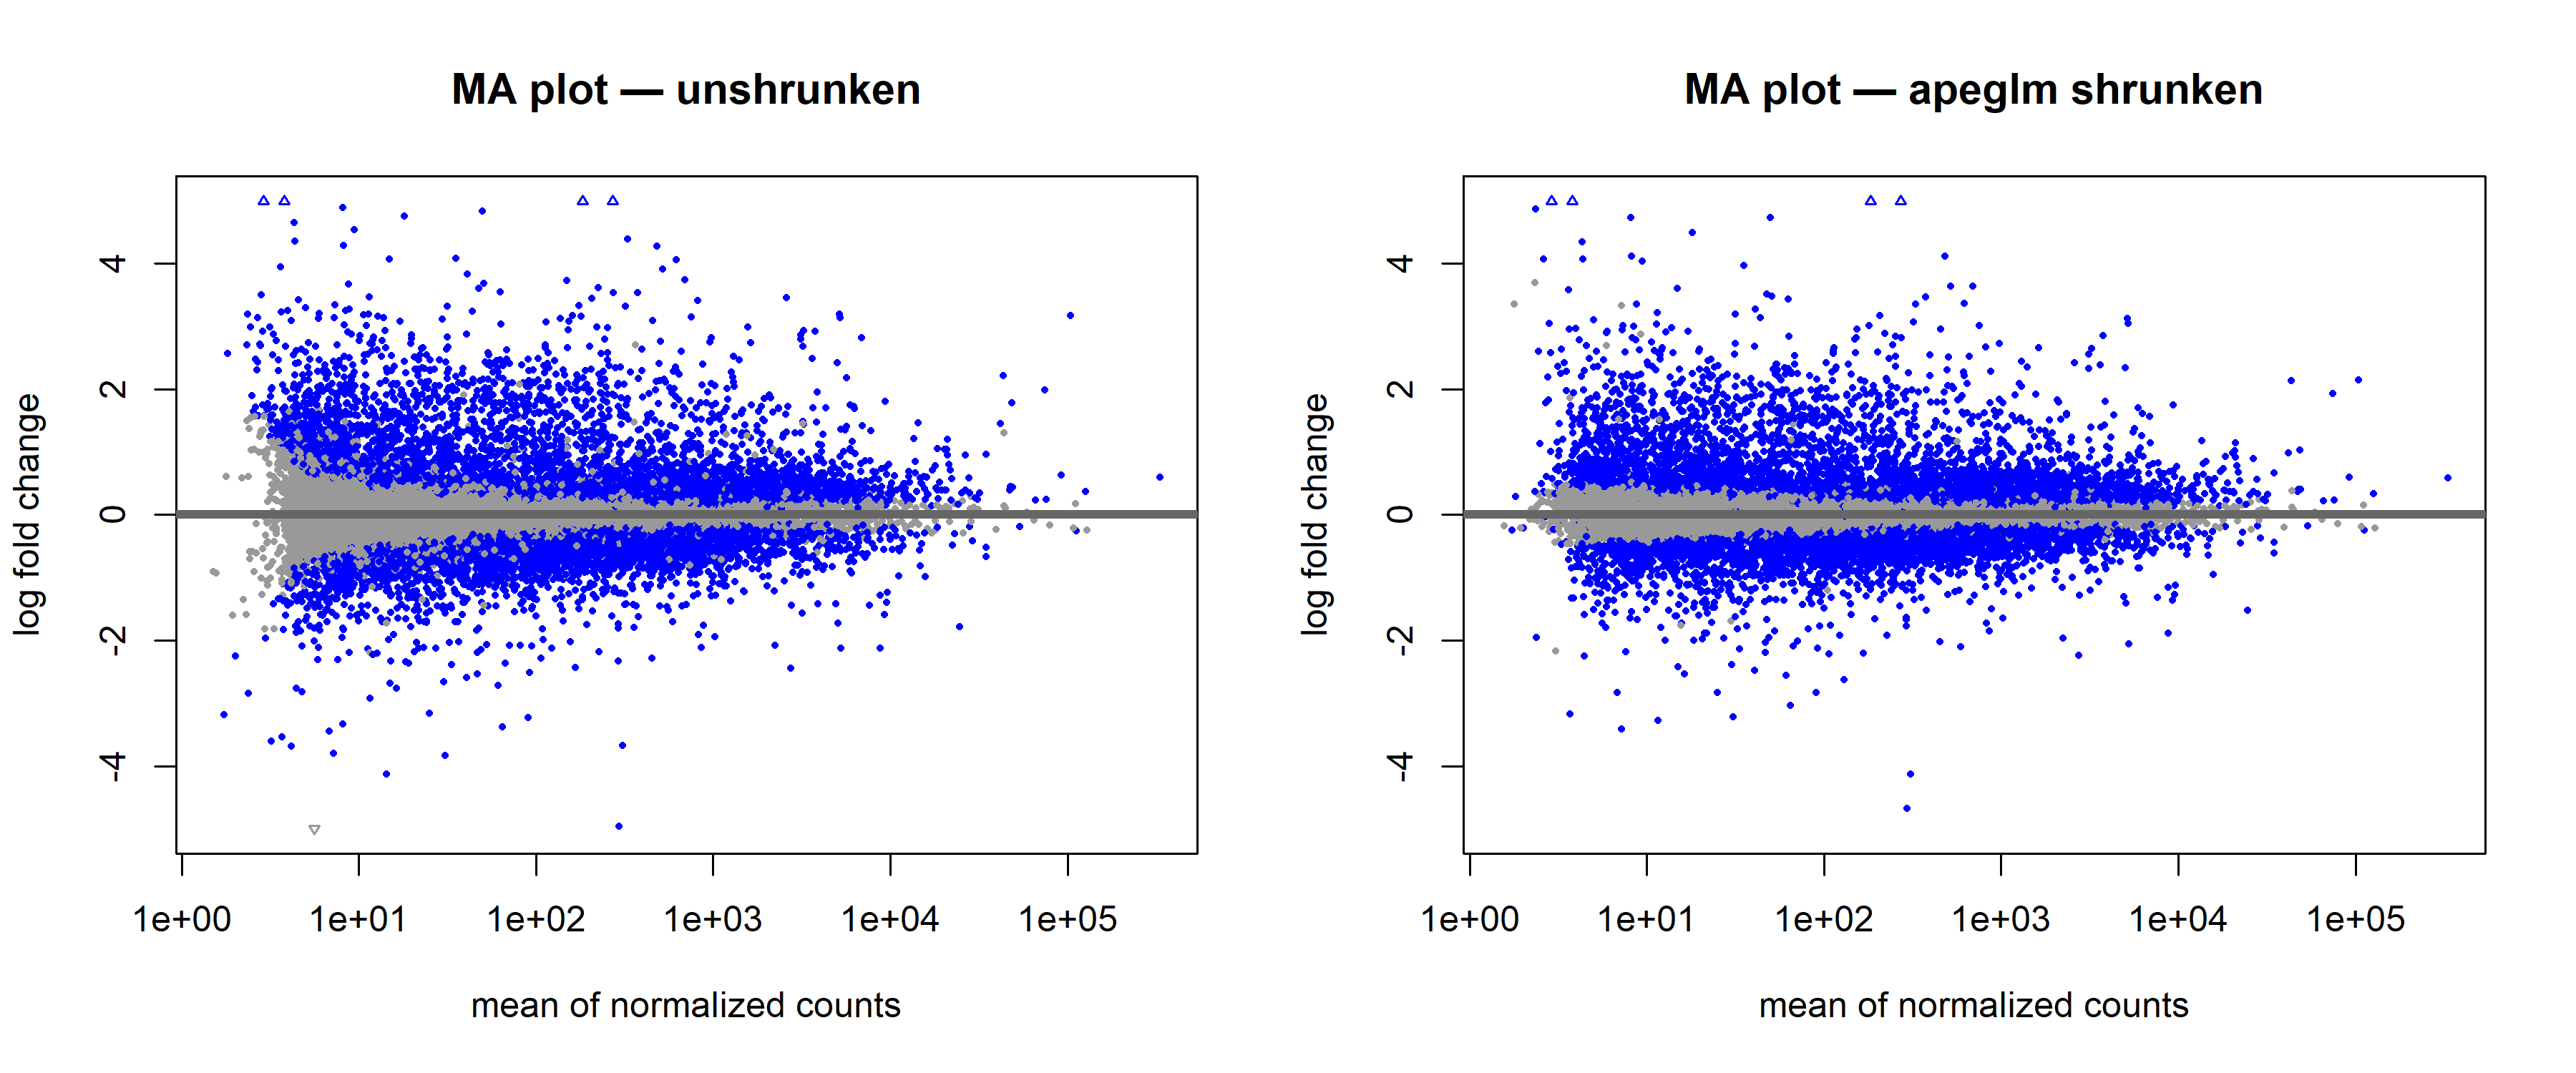
\includegraphics[width=\textwidth]{plots/phase8/phase8_MA_plots.png}
\end{center}

An MA plot shows each gene as a dot: x-axis = average expression level (mean of normalized
counts); y-axis = log$_2$ fold-change. The grey horizontal line is LFC = 0 (no change).
\textbf{Blue} dots are significant (\texttt{padj < 0.05}); grey dots are not significant.
Triangles at the top/bottom are points outside the y-axis limits.

\textit{Left — unshrunken LFCs:}
\begin{itemize}[nosep]
  \item At the far left (very low mean counts, $\sim$1--10), the dots scatter wildly across
        the full $\pm$5 range. These are noisy genes where a few counts difference
        between groups appears as a huge fold-change.
  \item There are several blue dots at very low mean counts — genes called significant
        despite being lowly expressed. These are unreliable: any small fluctuation
        inflates the LFC for a gene with only 2--5 counts per sample.
  \item At higher mean counts ($\geq 100$), the cloud narrows and converges toward 0,
        which is the expected pattern for genes that are not DE.
\end{itemize}

\textit{Right — apeglm shrunken LFCs:}
\begin{itemize}[nosep]
  \item The low-count dots on the left are pulled back toward 0. The cloud at
        the left edge is now narrow and flat — the noisy LFCs have been shrunk.
  \item The triangles (most extreme outliers) are unchanged because they correspond to
        high-count, genuinely extreme DE genes whose LFCs are already trustworthy.
  \item \textbf{The right-side (high mean) results are nearly identical between the two
        panels} — shrinkage only affects lowly expressed, noisy genes. For well-measured
        genes, the LFC does not change because there is enough data to estimate it precisely.
\end{itemize}

\textbf{The key message from this pair of plots:} shrinkage does not remove true signal —
it removes noise from genes we have no power to measure reliably.
All downstream results (volcano, heatmap, boxplots) use the shrunken LFCs.

\subsection{Volcano plot}

\begin{center}
  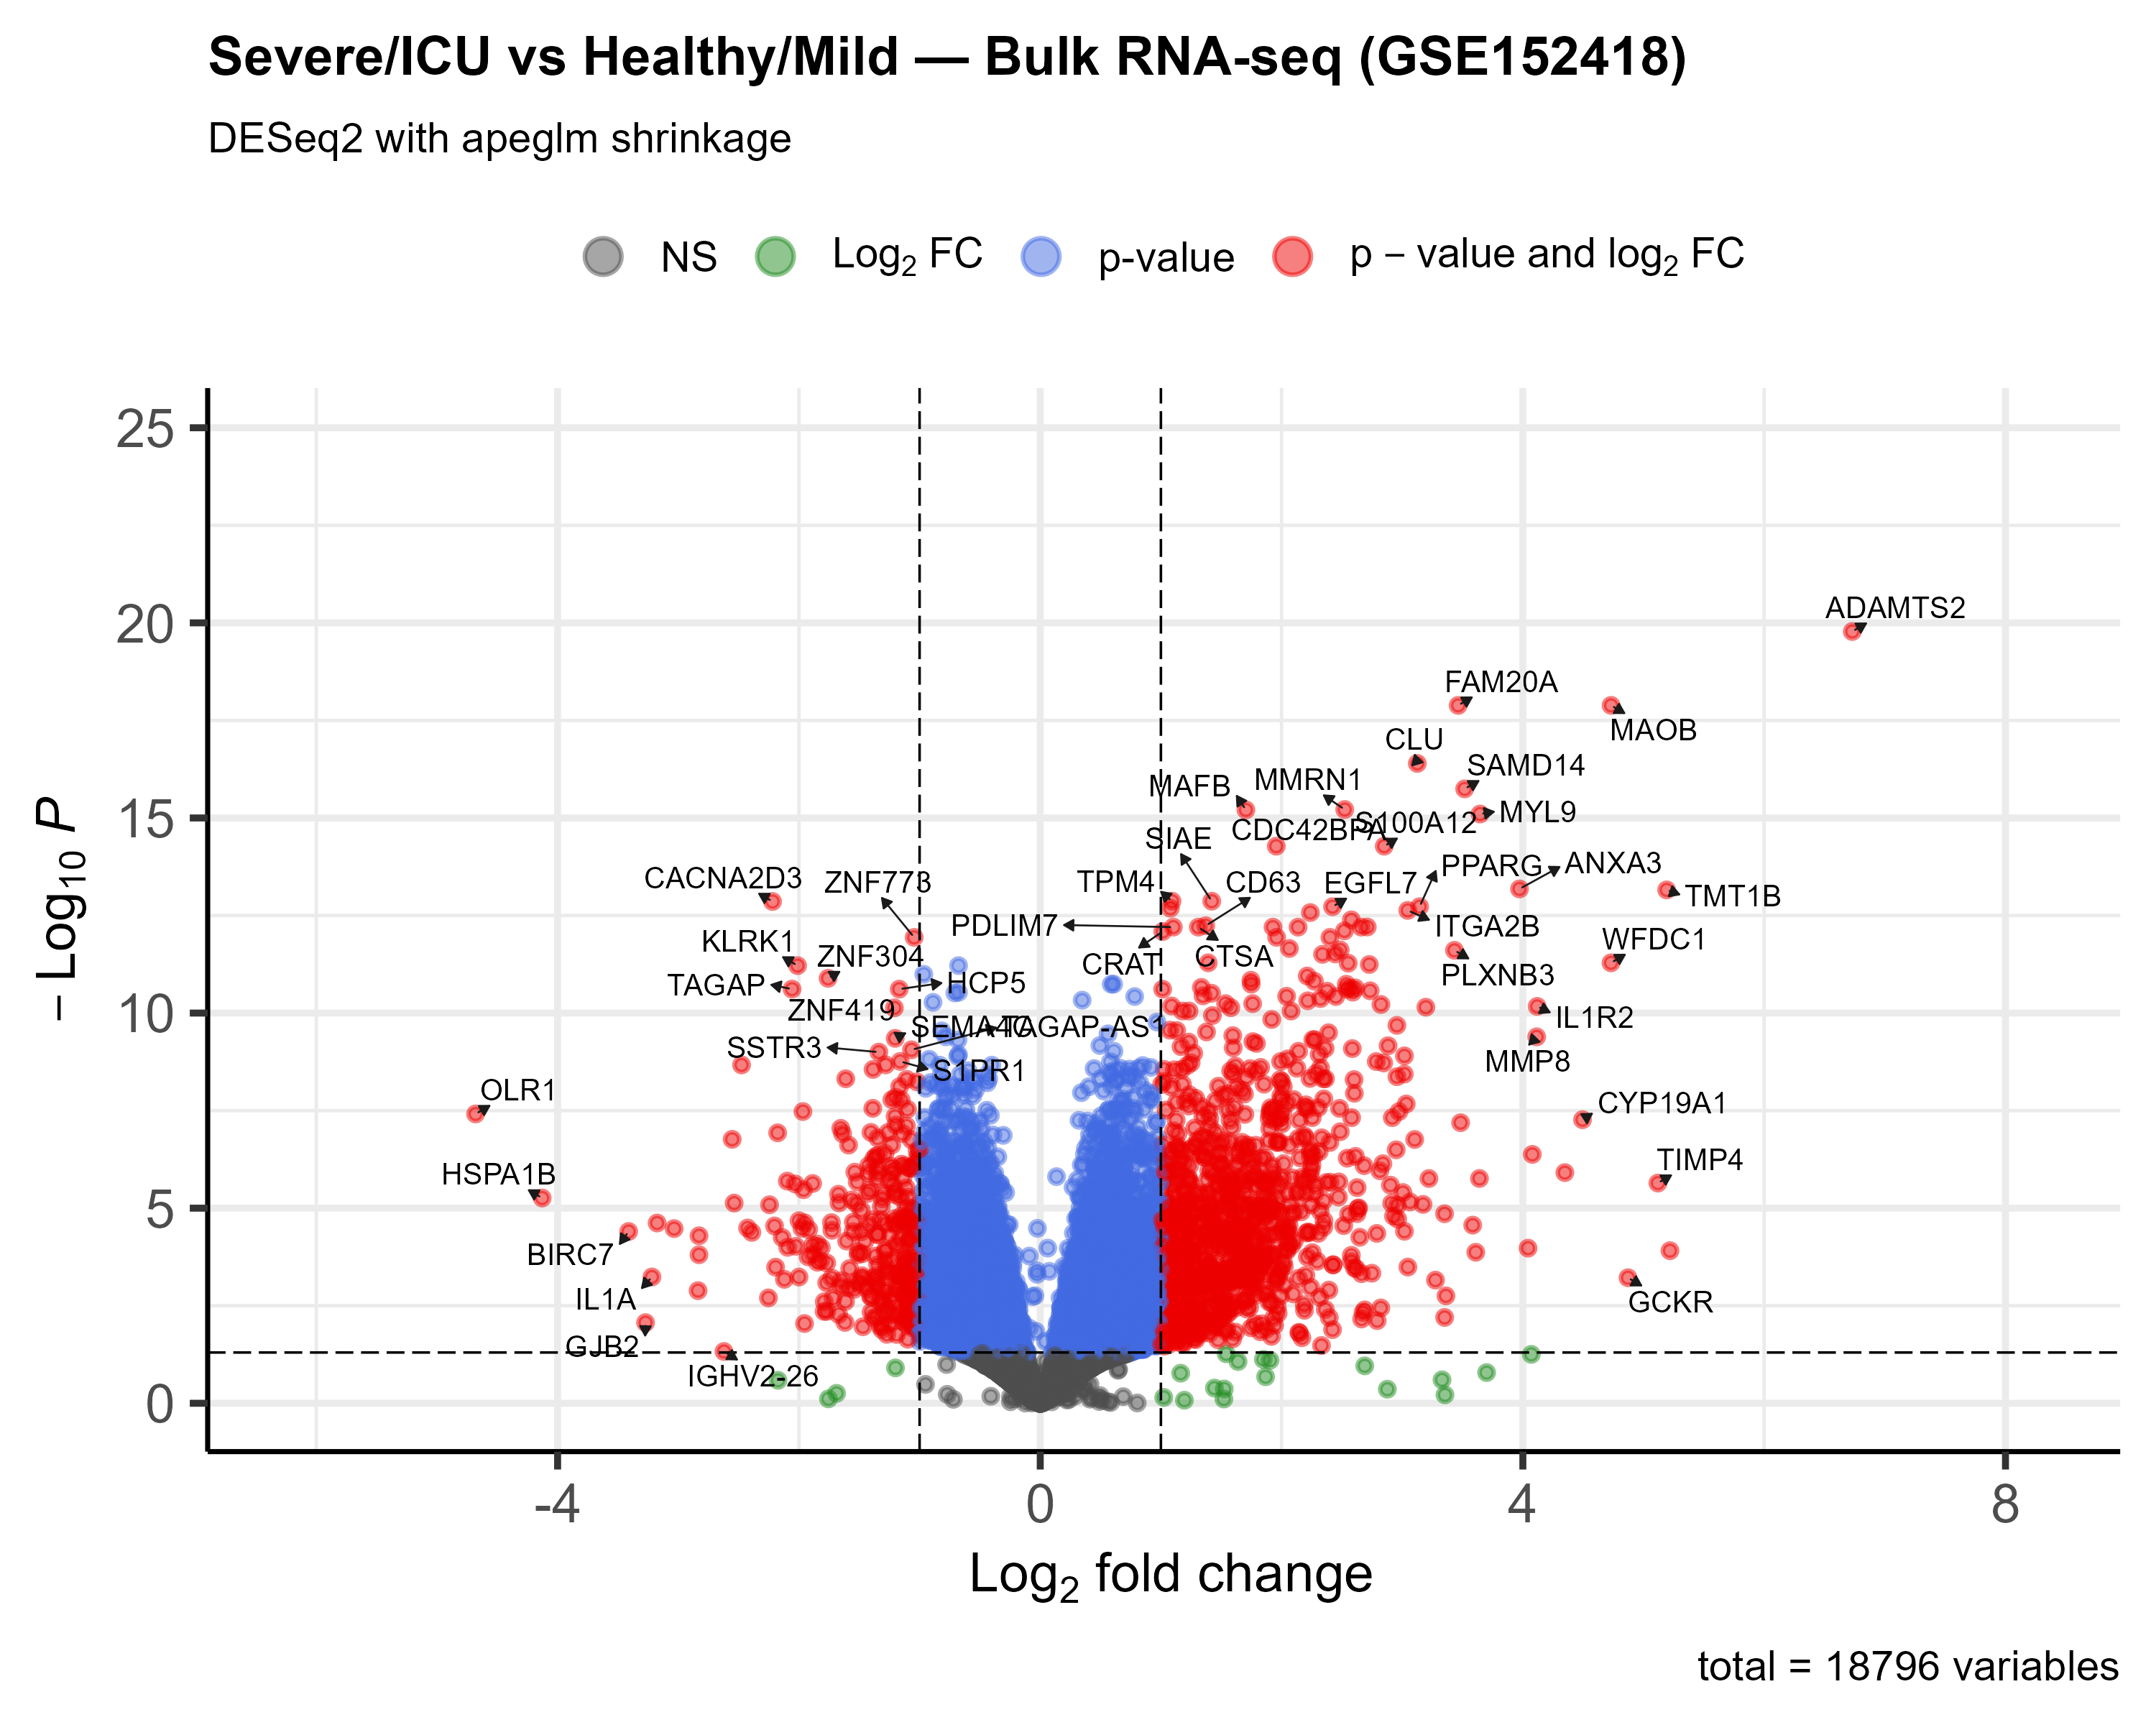
\includegraphics[width=\textwidth]{plots/phase8/phase8_volcano.png}
\end{center}

x-axis = log$_2$ fold-change (Severe/ICU vs Healthy/Mild);
y-axis = $-\log_{10}$(adjusted p-value).
Dashed vertical lines at $\pm$1 (twofold change cutoff).
Dashed horizontal line at padj = 0.05.
\textbf{Red} = significant in both fold-change and p-value.
\textbf{Blue} = significant in p-value only (within the $\pm$1 LFC window).
\textbf{Grey} = not significant.

\textit{The most significant upregulated genes (top-right):}
\begin{itemize}[nosep]
  \item \textbf{ADAMTS2} ($-\log_{10}P \approx 21$, LFC $\approx +8$) — the single
        most significant gene. ADAMTS2 is a collagen-processing protease expressed
        by macrophages and monocytes; its extreme upregulation in Severe/ICU blood
        points to extracellular matrix remodeling in severe disease.
  \item \textbf{FAM20A, MAOB, SAMD14, MMRN1} — all highly upregulated and significant.
        \textit{MMRN1} and \textit{ITGA2B} are platelet proteins; \textit{MAOB} is
        expressed in platelets and monocytes. Their co-upregulation suggests
        a \textbf{platelet activation signature} is prominent in severe COVID whole blood.
  \item \textbf{S100A12} — an alarmin (danger signal) produced by neutrophils and
        emergency myeloid progenitors; a marker of \textbf{emergency granulopoiesis}
        in severe infection.
  \item \textbf{IL1R2} (IL-1 receptor decoy) — a surprise: rather than IL-1$\beta$
        itself being upregulated, the \textit{decoy receptor} that inhibits IL-1 signaling
        is upregulated. This is the bulk-level echo of the inflammatory / counter-regulatory
        balance seen at the single-cell level in Phase 4.
  \item \textbf{MMP8, ANXA3, PLXNB3, WFDC1, TMT1B} — inflammatory proteases,
        cytoskeletal proteins, and myeloid-associated proteins further filling the
        upregulated landscape.
\end{itemize}

\textit{The most significant downregulated genes (top-left):}
\begin{itemize}[nosep]
  \item \textbf{OLR1} (LOX-1, $-\log_{10}P \approx 8$) — an oxidized LDL receptor
        expressed on NK cells and T cells. Its strong downregulation reflects the
        \textbf{lymphocyte depletion} (NK cells, T cells) documented in Phase 4.
  \item \textbf{KLRK1} (NKG2D) — an NK cell activating receptor. NK cell depletion
        again.
  \item \textbf{TAGAP} — a T cell activation GTPase. T cell loss.
  \item \textbf{HSPA1B} — a heat shock protein expressed in stressed lymphocytes.
  \item \textbf{CACNA2D3, ZNF778, ZNF304} — zinc finger transcription factors
        expressed predominantly in lymphoid cells.
\end{itemize}

\textbf{The overall pattern:} the dominant bulk signal in severe COVID blood is
\textbf{not the monocyte ISG/IL-1$\beta$ programs from Phase 4} — it is the
downstream composition shift. The strongest upregulated genes are myeloid and
platelet markers; the strongest downregulated genes are lymphocyte markers.
This is the cell-dilution effect of bulk RNA-seq: the monocyte-specific programs
are mixed into a whole-blood average dominated by the expansion of myeloid and
platelet populations and the disappearance of lymphocytes.

\subsection{Heatmap of top 30 DE genes \small\normalfont\textit{(Step 14)}}

\begin{center}
  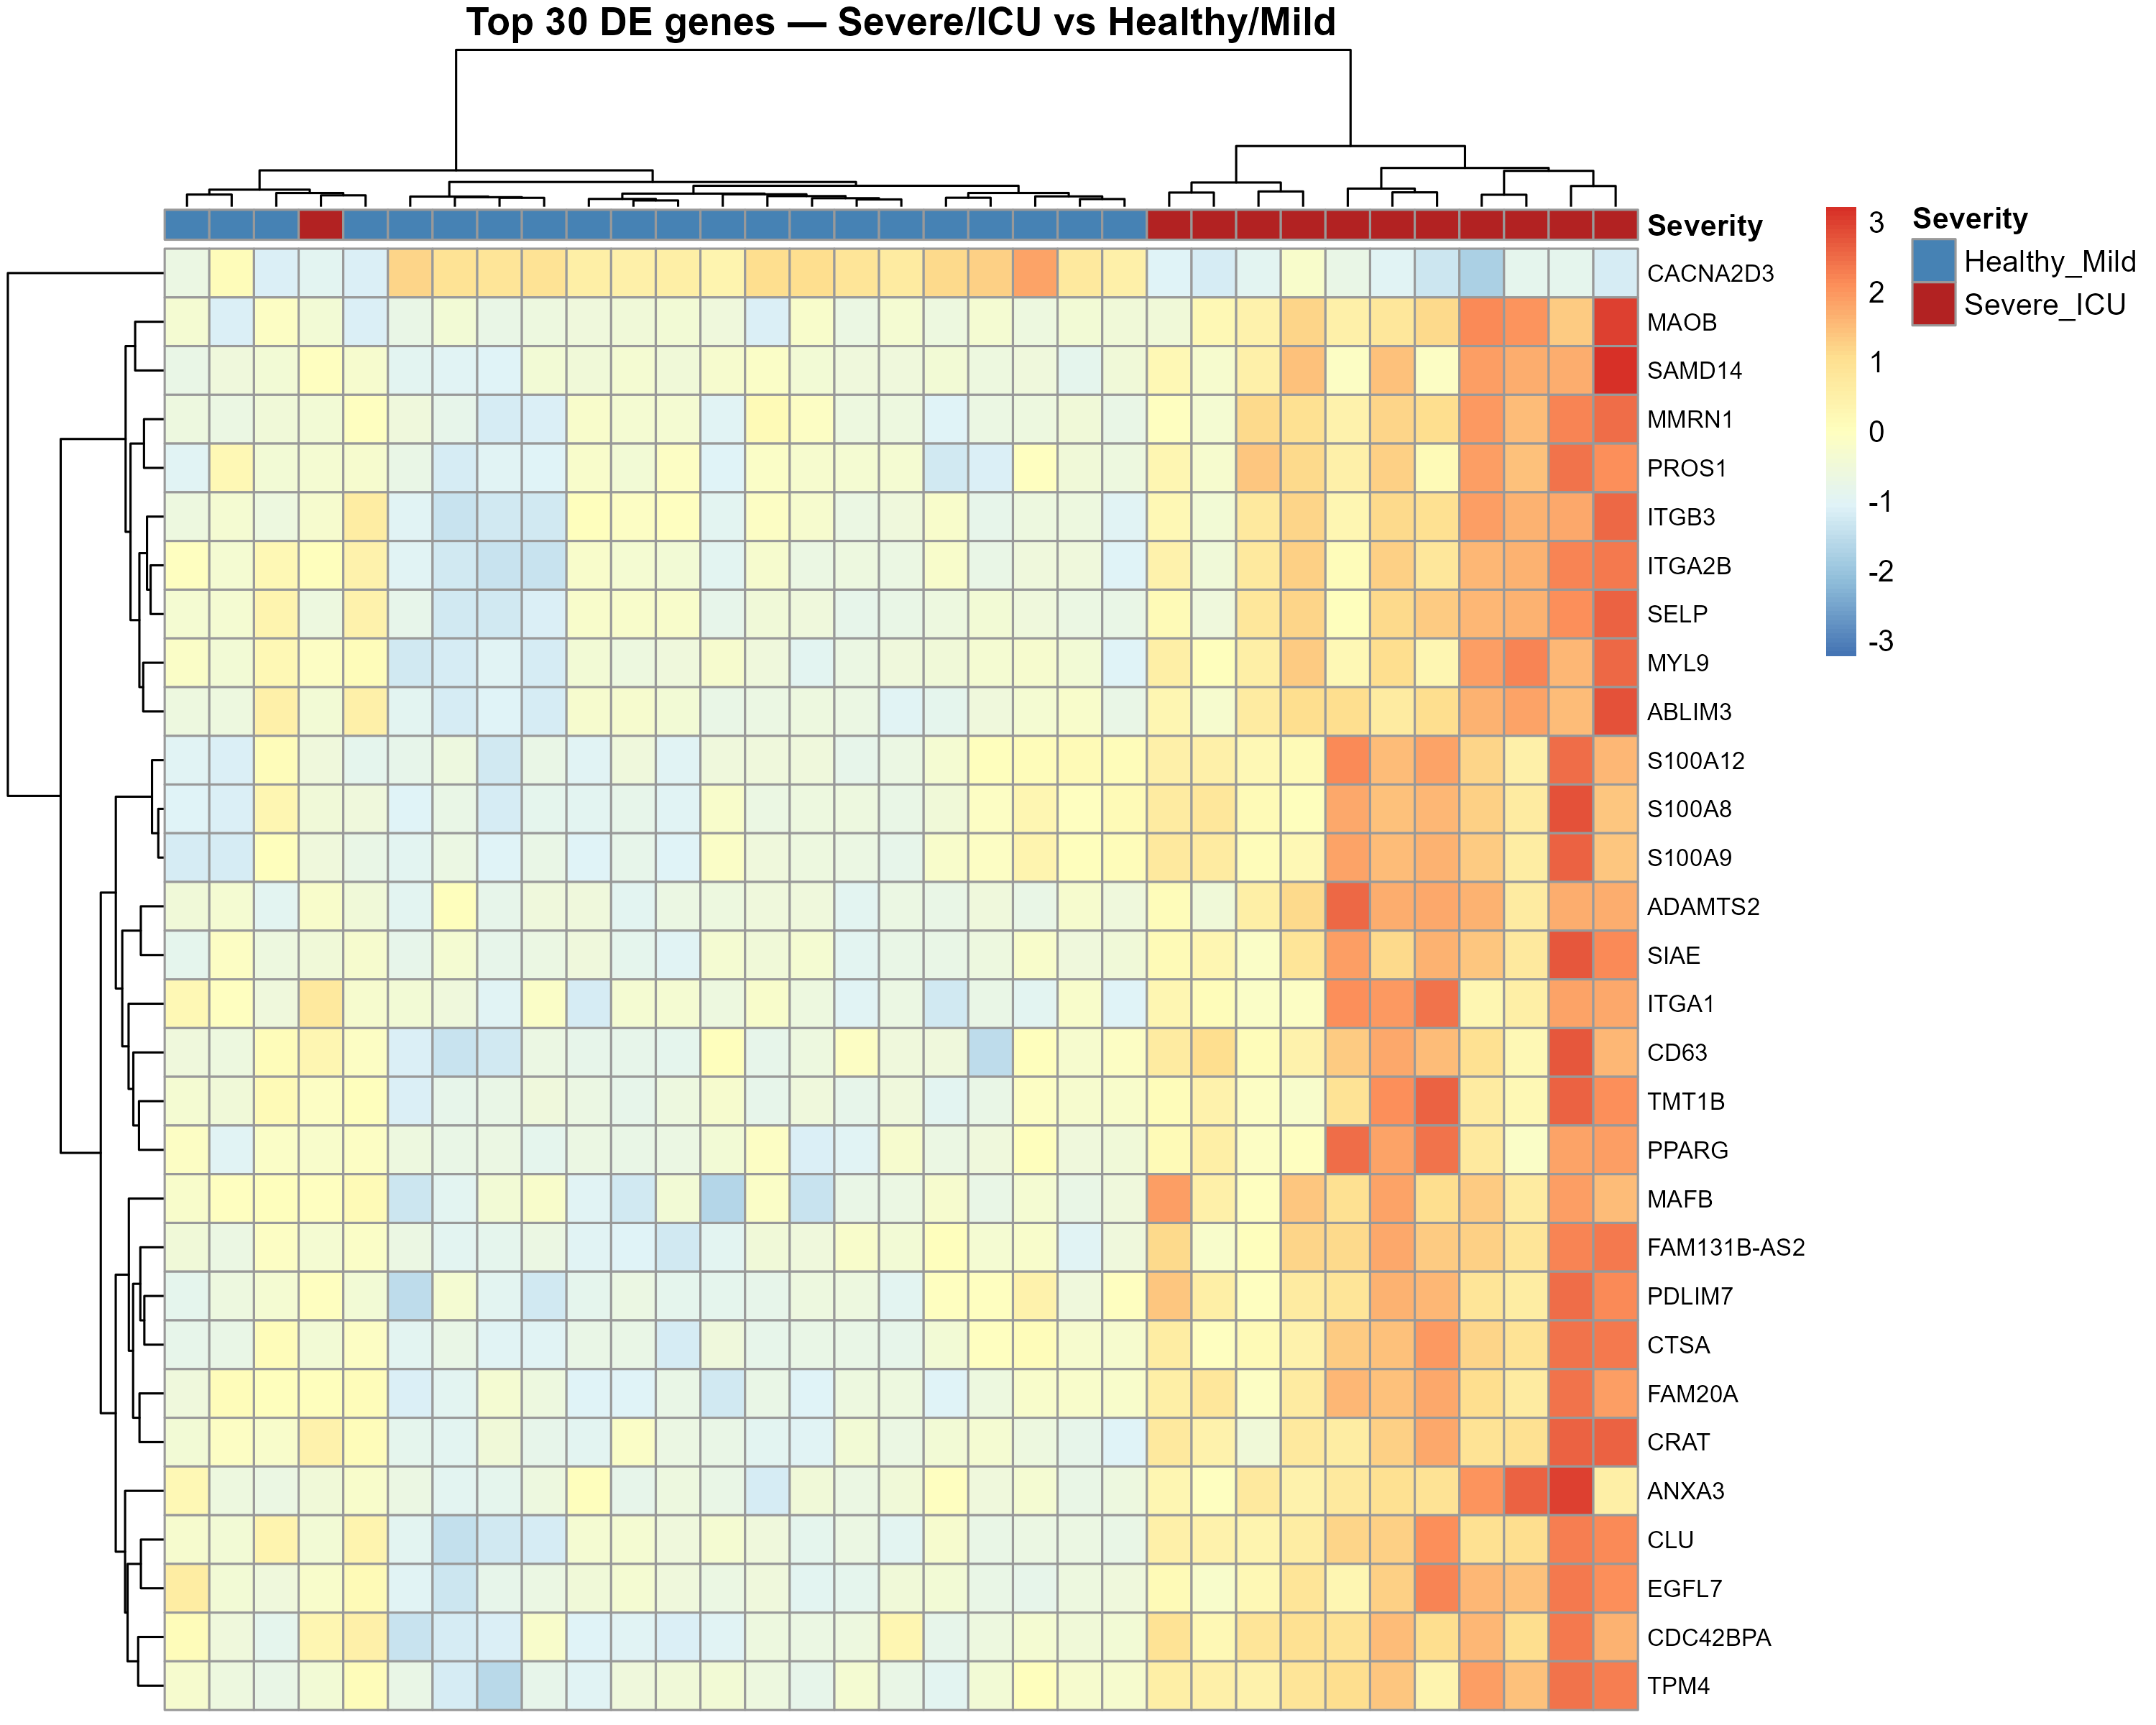
\includegraphics[width=\textwidth]{plots/phase8/phase8_heatmap_top30.png}
\end{center}

The heatmap shows the 30 most significantly DE genes, with samples on the
x-axis (unsupervised hierarchical clustering) and genes on the y-axis.
Row labels are gene symbols. Column annotation bars show severity group:
blue = Healthy\_Mild, red = Severe\_ICU. Colour scale: orange/red = high
scaled expression; blue = low.

\begin{itemize}[nosep]
  \item \textbf{Almost perfect severity separation:} the unsupervised hierarchical
        clustering (which knows nothing about group labels) places nearly all
        Severe/ICU samples in one block (right) and nearly all Healthy/Mild in
        another (left). This is strong evidence — the top 30 genes alone are
        sufficient to separate the two groups without any label information.
  \item \textbf{All top 30 genes are upregulated in Severe/ICU} (orange/red
        in the Severe block, blue in the Healthy block). This asymmetry is
        real: the most statistically extreme results in this dataset are all
        in the upregulation direction, consistent with the volcano.
  \item \textbf{Notable gene clusters} (from the row dendrogram):
        \begin{itemize}[nosep]
          \item Top cluster (CACNA2D3, MAOB, SAMD14, MMRN1, PROS1, ITGB3,
                ITGA2B, SELP, MYL9, ABLIM3) — all platelet and
                coagulation-related proteins. Platelet activation is the
                single strongest biological signal at the bulk level.
          \item Middle cluster (S100A12, S100A8, S100A9, ADAMTS2) — alarmin
                proteins and matrix remodeling; emergency myeloid response.
          \item Lower cluster (MAFB, PPARG, CD63, CTSA, FAM20A, ANXA3,
                CLU, CRAT, PDLIM7) — monocyte/macrophage differentiation genes.
                \textit{MAFB} and \textit{PPARG} are transcription factors
                driving monocyte-to-macrophage transition. \textit{CD63}
                is a lysosomal membrane protein upregulated on activated monocytes.
        \end{itemize}
  \item \textbf{One Healthy\_Mild outlier sample} in the top-right appears with
        moderately orange color — a Healthy/Mild sample whose gene expression
        pattern partially resembles the Severe group. This sample may be from
        a donor with an elevated inflammatory baseline or a pre-existing condition.
        It is not sufficient to change the overall result.
\end{itemize}

\subsection{Key gene boxplots — do the monocyte-program genes change in bulk? \small\normalfont\textit{(Step 15)}}

\begin{center}
  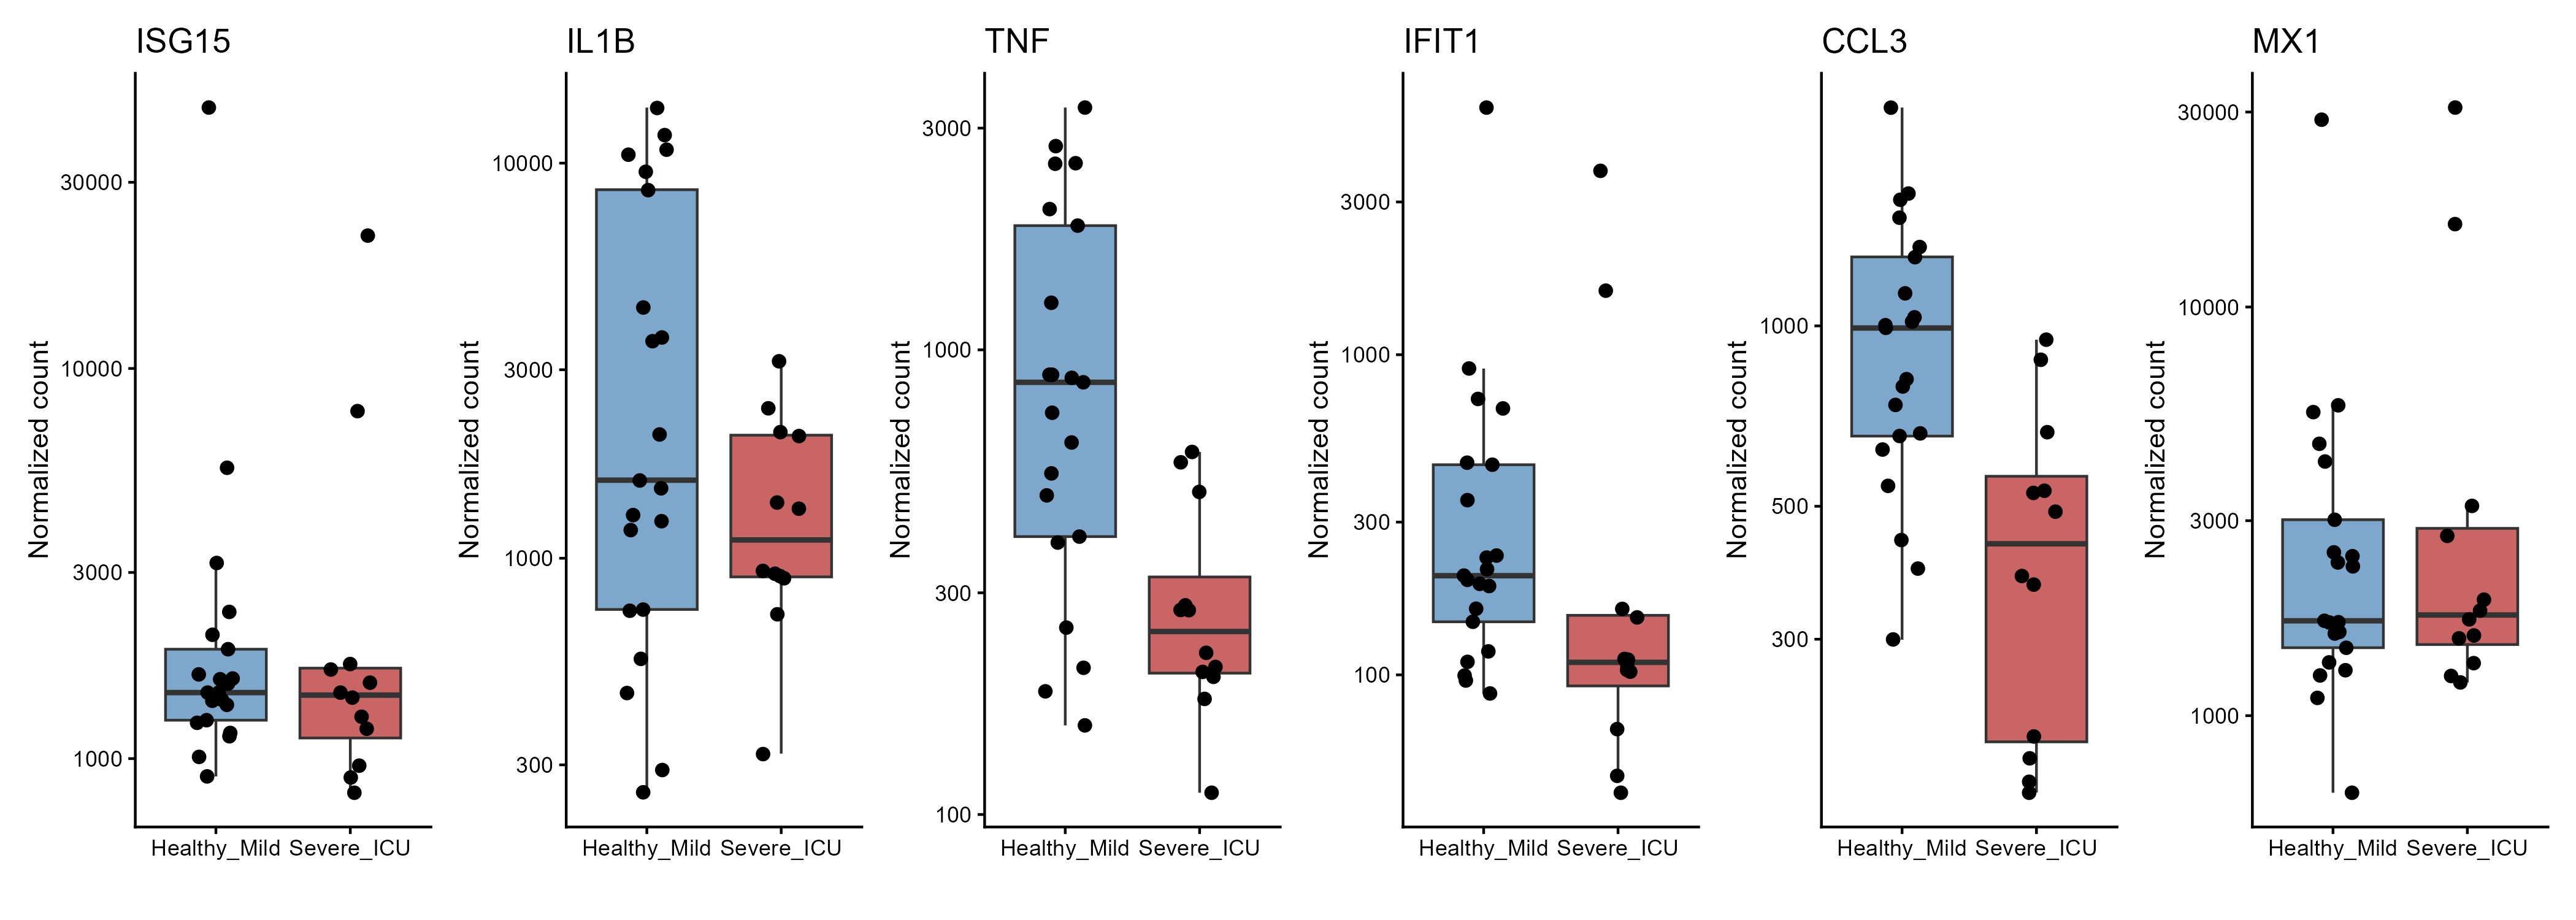
\includegraphics[width=\textwidth]{plots/phase8/phase8_key_gene_boxplots.png}
\end{center}

These six genes were chosen because they are the core of the ISG and TNF/IL-1$\beta$
modules from Phases 4 and 5. Each boxplot shows the normalized count in
Healthy\_Mild (blue) vs Severe\_ICU (red) on a log scale. Each dot is one sample.

\begin{itemize}[nosep]
  \item \textbf{ISG15:} Healthy\_Mild and Severe\_ICU are nearly identical — both have
        a median around 1,400. One outlier Healthy/Mild sample has extremely high ISG15
        (30,000), drastically elevating the Healthy/Mild variance. No upward shift in
        Severe. \textbf{ISG15 is not elevated in Severe COVID whole blood.}

  \item \textbf{IL1B:} Counter-intuitively, the Healthy\_Mild median ($\sim$1,500) is
        \textit{higher} than Severe\_ICU ($\sim$1,100), with wide variance in both groups.
        \textbf{IL1B is not upregulated in Severe COVID whole blood.}

  \item \textbf{TNF:} Again Healthy\_Mild has a higher median ($\sim$800) than
        Severe\_ICU ($\sim$200). \textbf{TNF is lower in Severe COVID whole blood.}

  \item \textbf{IFIT1:} Healthy\_Mild slightly higher. Not upregulated in Severe.

  \item \textbf{CCL3:} Healthy\_Mild higher median ($\sim$900) vs Severe ($\sim$500).
        Lower in Severe.

  \item \textbf{MX1:} The two groups are essentially the same, with overlapping boxes
        and similar medians.
\end{itemize}

\textbf{This is the most important result of Phase 8.}
Every single gene that was elevated in severe COVID \textit{monocytes} in Phase 4
is \textbf{not elevated — and in several cases is lower} — in severe COVID
\textit{whole blood}.

Why? Because bulk RNA-seq mixes all cell types together. In severe COVID:
\begin{itemize}[nosep]
  \item Monocytes expand — they are a bigger fraction of the blood.
  \item But the monocytes that produce IL1B are a specific sub-cluster
        (Cluster 7 in Phase 3), not all monocytes.
  \item Lymphocytes (T cells, NK cells, B cells) are depleted — their contribution
        to the whole-blood signal shrinks.
  \item T cells and NK cells also produce ISG genes, TNF, and CCL3 in healthy individuals.
        Their loss in severe COVID \textit{reduces} the whole-blood signal of these genes
        even while monocyte production of them may be going up.
\end{itemize}

The net effect is cancellation: the monocyte upregulation is overwhelmed by the
cross-cellular compositional shift. This is the fundamental limitation of bulk RNA-seq
for cell-type-specific questions — and it is exactly why single-cell RNA-seq was
needed in Phases 1--6 to find the co-activated monocyte state in the first place.

\subsection{Phase 8 conclusion}

Phase 8 asked: \textit{which genes are different in whole blood between Severe/ICU
and Healthy/Mild COVID?} The answers are:

\begin{enumerate}[nosep]
  \item \textbf{The top bulk signal is myeloid expansion and platelet activation,
        not monocyte inflammatory programs.}
        The most significant upregulated genes (ADAMTS2, MMRN1, ITGA2B, SELP,
        S100A12, S100A8/9, MAFB) are markers of platelets, emergency myeloid progenitors,
        and monocyte-to-macrophage transition — not the ISG or IL-1$\beta$ programs
        that drove the single-cell analysis.

  \item \textbf{The top downregulated signal is lymphocyte depletion.}
        OLR1, KLRK1, TAGAP, CACNA2D3 — all lymphocyte markers, consistent
        with the lymphopenia documented at the single-cell level in Phase 4.

  \item \textbf{The monocyte-specific genes (ISG15, IL1B, TNF, IFIT1, CCL3, MX1)
        are NOT upregulated in bulk blood.}
        This confirms the prediction from Phase 7: the monocyte programs are
        diluted by the whole-blood mix. Single-cell resolution was necessary
        to detect them.

  \item \textbf{The top 30 DE genes perfectly segregate samples by severity}
        (heatmap), showing the bulk signal is real and reproducible across donors
        — just biologically different from what the single-cell data showed.
\end{enumerate}

\textbf{What this means for the story:}
The single-cell finding (co-activated monocytes) and the bulk finding (platelet/myeloid
expansion + lymphopenia) are \textit{complementary}, not contradictory.
They are different views of the same disease, at different levels of resolution.
Phase 9 will ask whether the bulk results change once we correct for the gender
imbalance flagged in Phase 7.

% ─────────────────────────────────────────────
\section{Phase 9 — Adjusting for Gender as a Confounder}
% ─────────────────────────────────────────────

\subsection{Phase 9 overview — the big picture}

\textbf{Phase 8 found the DE genes. Phase 9 checks that the finding is real and not driven by gender.}

In Phase 7 we flagged a problem: the Healthy\_Mild group is female-majority (13F/8M),
while the Severe\_ICU group is male-majority (5F/7M). Males on average have worse
COVID outcomes, meaning some genes that are male- or female-biased could appear
as COVID-severity genes in Phase 8 — not because they are about COVID, but because
of the gender imbalance.

The fix is simple: re-run DESeq2 with the extended model
\texttt{\textasciitilde\ gender + severity\_group}.
This tells DESeq2: ``account for gender differences first, then measure the severity
effect on top of that.''

If the Phase 8 results hold up after this correction, the DE genes are genuine
severity effects. If they collapse, gender was the real driver, not COVID.
Phase 9 has two outputs: the corrected model's MA plot, and a direct comparison
of the two models' fold-changes.

\subsection{Gender balance check \small\normalfont\textit{(Step 3)}}

\begin{center}
  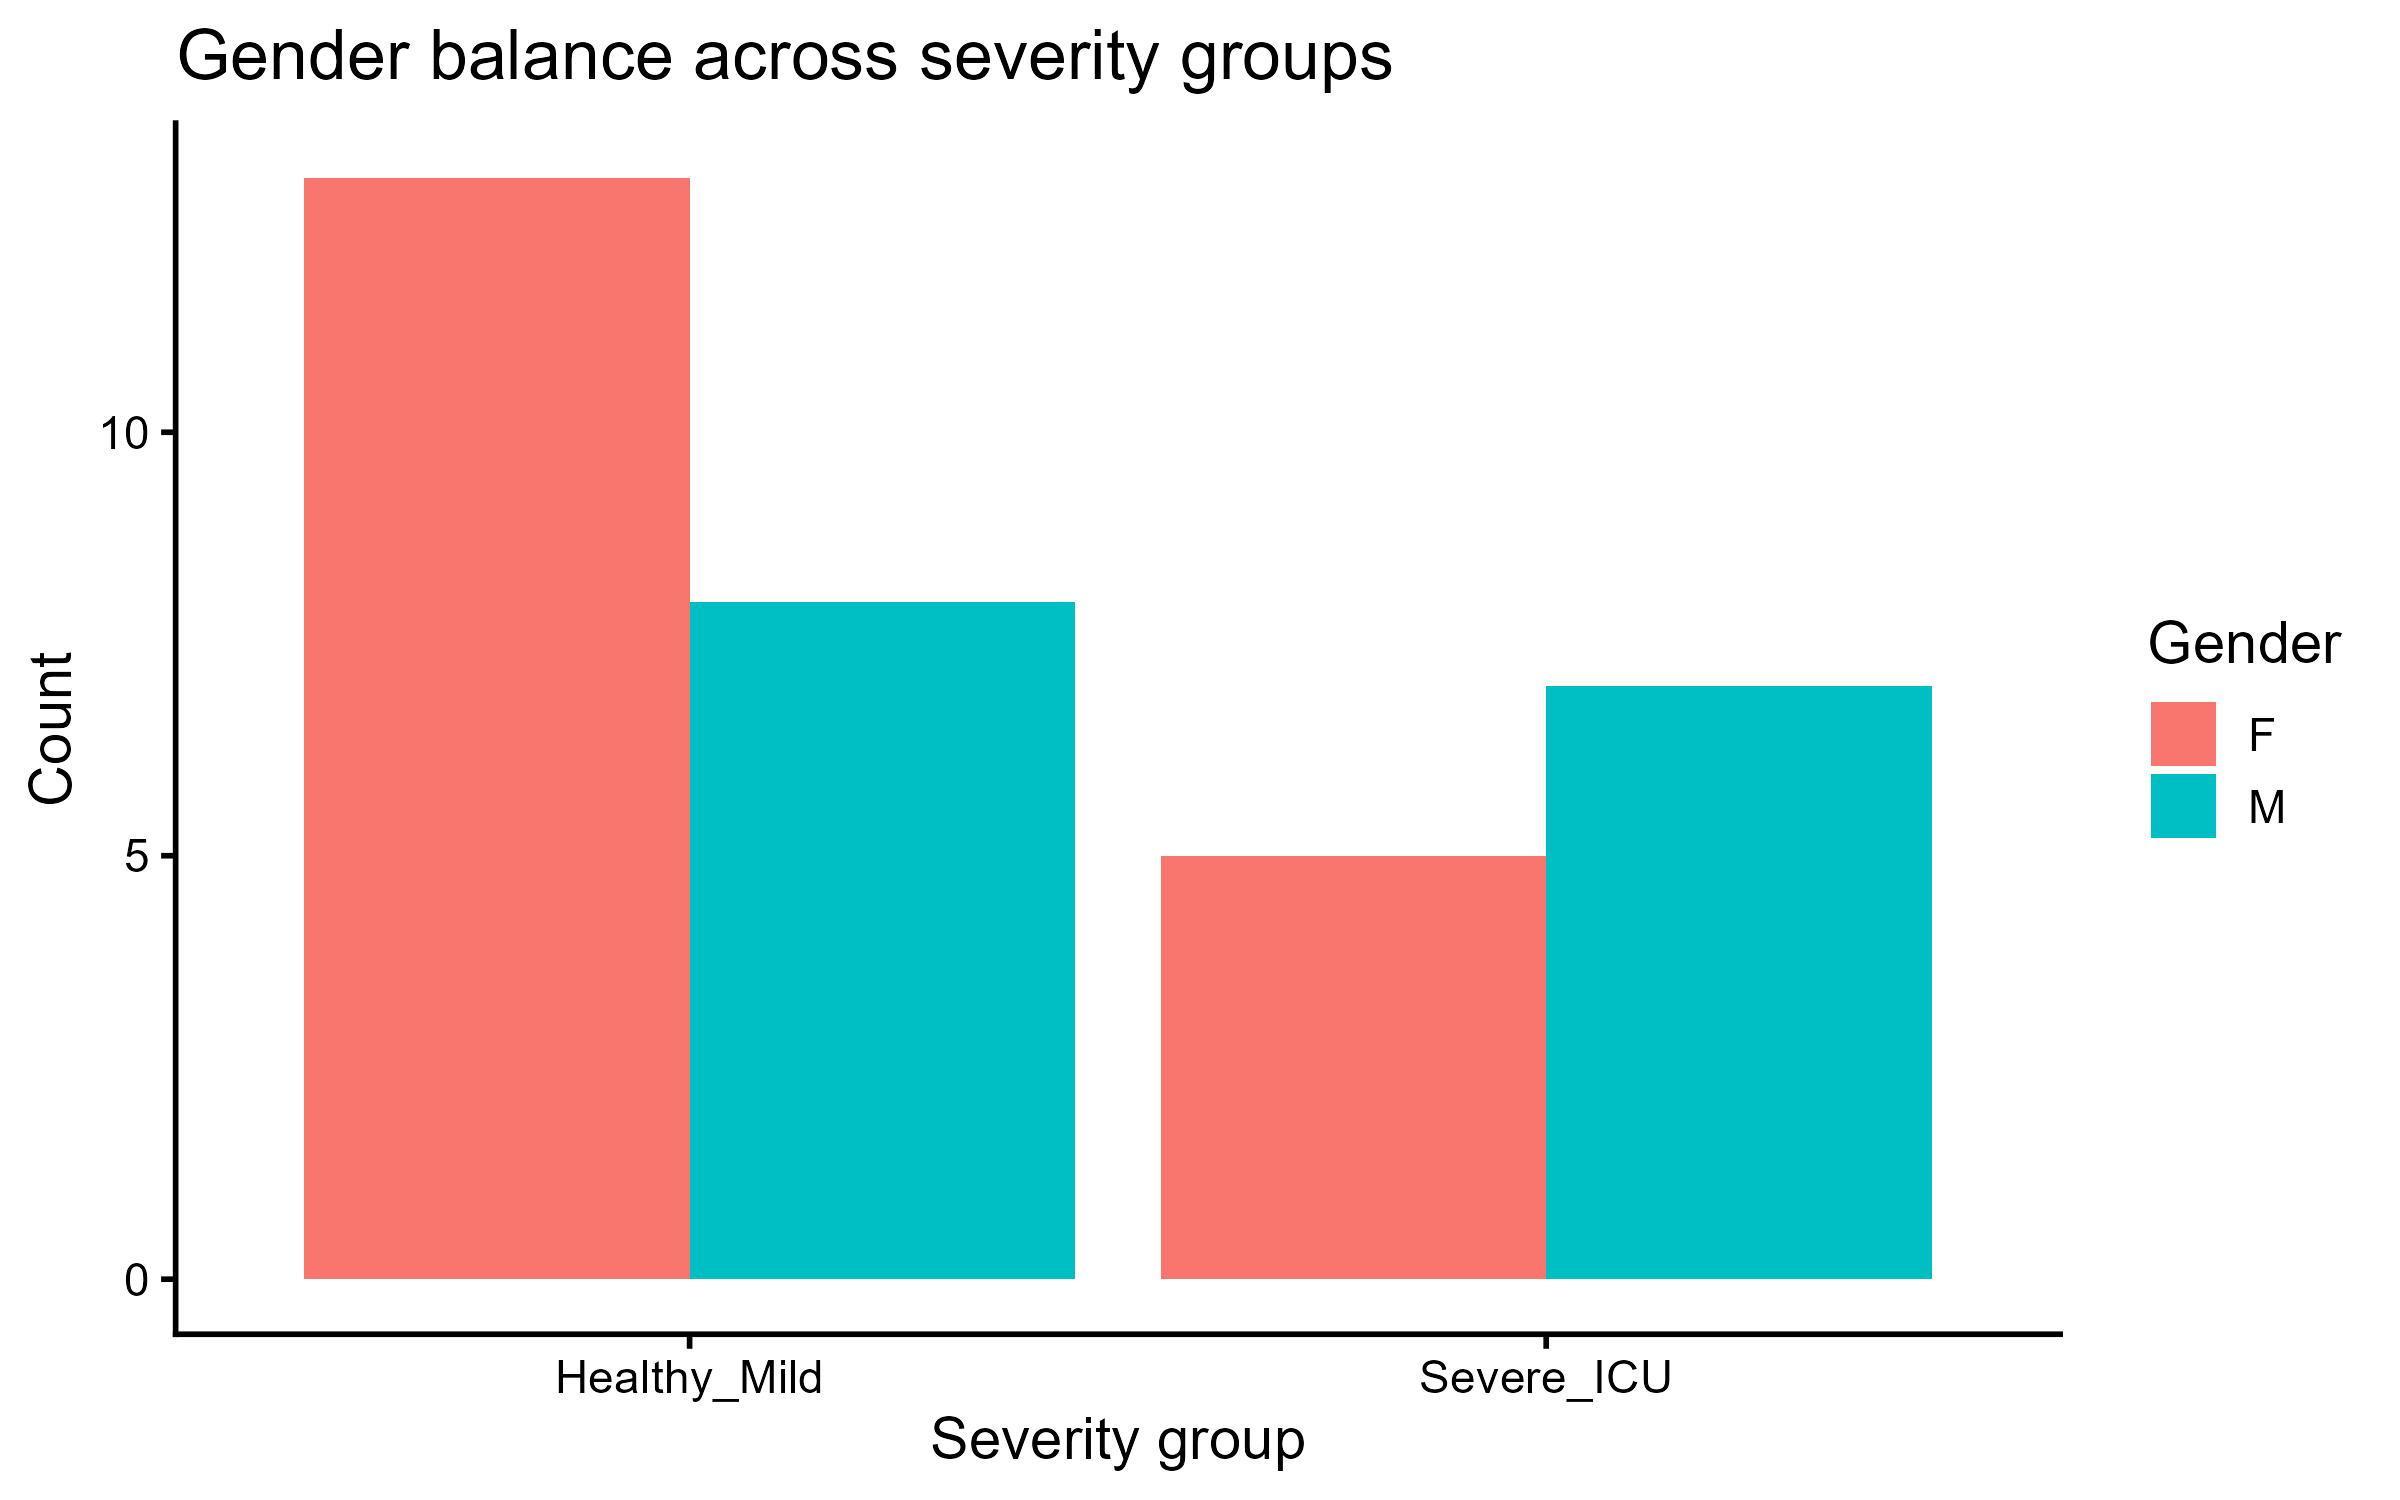
\includegraphics[width=0.75\textwidth]{plots/phase9/phase9_gender_balance.png}
\end{center}

The barplot confirms the imbalance flagged in Phase 7:

\begin{itemize}[nosep]
  \item \textbf{Healthy\_Mild:} 13 Female (salmon), 8 Male (teal) — 62\% female.
  \item \textbf{Severe\_ICU:} 5 Female, 7 Male — 58\% male.
\end{itemize}

The two groups have \textit{opposite} gender majorities.
This is the textbook definition of a confounder: a variable (gender) that is
correlated with both the exposure (severity) and the outcome (gene expression).
The chi-squared test on this 2×2 table tests whether this association is
statistically significant — if $p < 0.05$, the imbalance is too large to ignore.

The action taken here is correct: rather than excluding samples or trying to
match groups by gender (which would reduce sample size further), we include
gender as a covariate in the DESeq2 model.
This is the standard approach in clinical genomics studies with unbalanced covariates.

\subsection{DESeq2 adjusted model and MA comparison \small\normalfont\textit{(Steps 4–6)}}

DESeq2 is re-run with the extended design formula
\texttt{\textasciitilde\ gender + severity\_group}.
Size factors from Phase 8 are reused so that the only change is the addition
of the gender term.

\subsubsection*{Side-by-side MA plots — simple vs adjusted model}

\begin{center}
  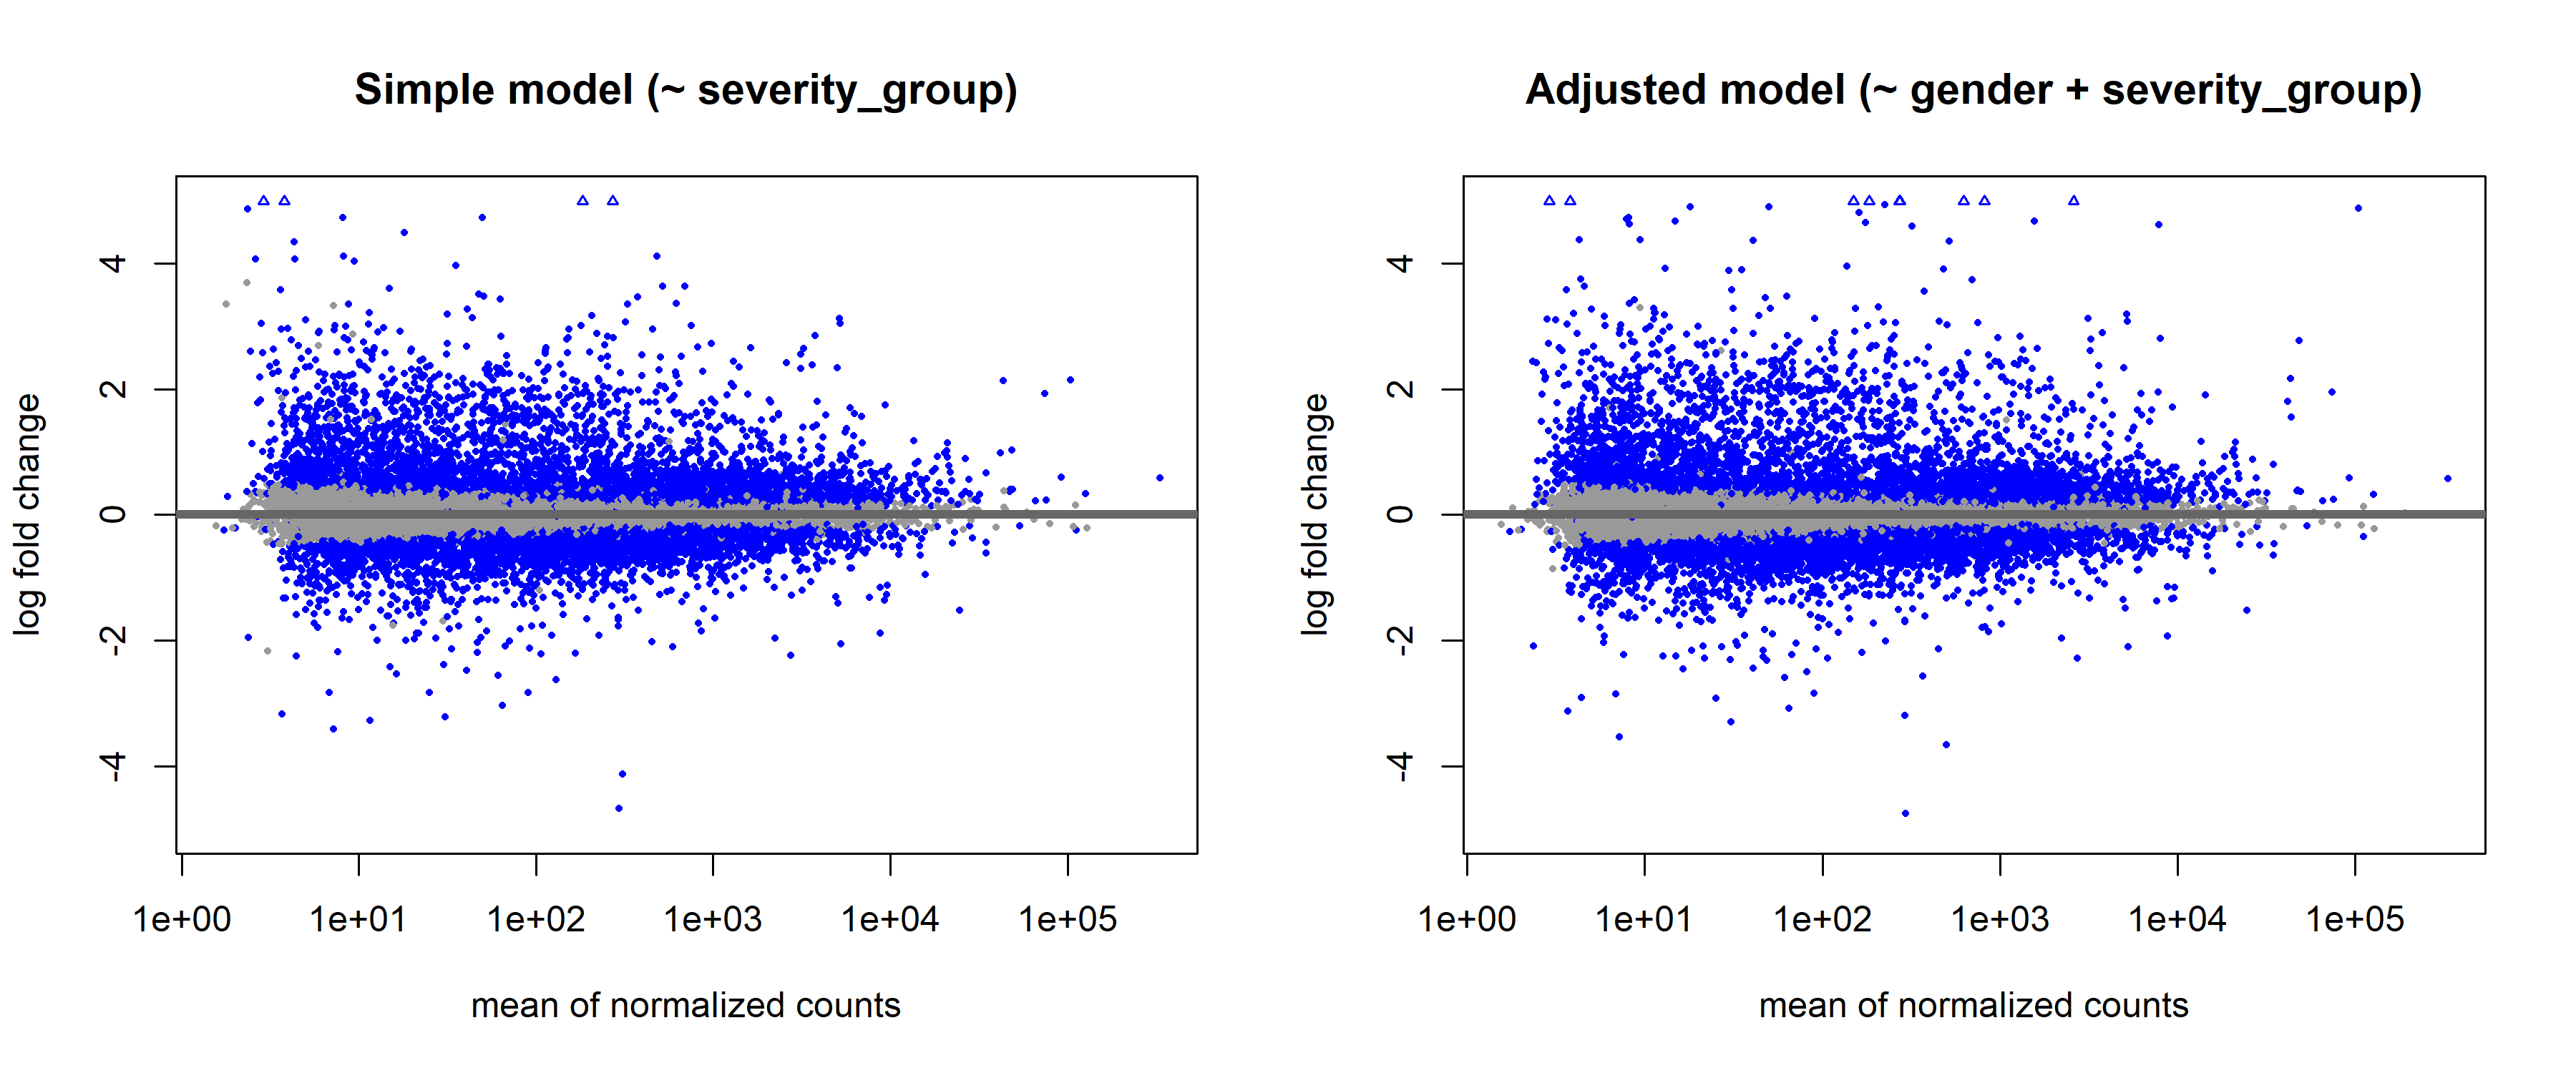
\includegraphics[width=\textwidth]{plots/phase9/phase9_MA_comparison.png}
\end{center}

Left panel = Phase 8 simple model (\texttt{\textasciitilde\ severity\_group}).
Right panel = Phase 9 adjusted model (\texttt{\textasciitilde\ gender + severity\_group}).
In both plots: blue = significant (\texttt{padj < 0.05}); grey = not significant.

\begin{itemize}[nosep]
  \item \textbf{The overall shape is nearly identical between the two panels.}
        Both show the same fan of blue dots spreading upward and downward from
        zero across the full expression range ($10^0$ to $10^5$).
        The density of significant genes, their spread, and the overall
        signal-to-noise structure look the same.

  \item \textbf{The top-triangle outliers (truncated high-LFC genes)} appear in
        the same positions in both panels — the same extreme genes survive the
        adjustment. These are the strongest, most robust DE results.

  \item \textbf{The adjusted model has slightly more significant genes} (slightly
        more blue in the right panel, particularly at moderate expression levels
        $10^2$--$10^4$). This is expected: by accounting for gender variation,
        DESeq2 reduces within-group noise, which increases statistical power for
        the severity effect. Adding a confounder that explains some of the
        residual variance often improves, rather than reduces, the number of
        detectable DE genes.

  \item \textbf{No dramatic loss of significant genes.} If gender had been the
        real driver of Phase 8's findings, the adjusted MA plot would show fewer
        blue dots — genes would drop to grey after correcting for gender.
        That does not happen. The significant landscape is preserved.
\end{itemize}

\subsection{LFC correlation between models \small\normalfont\textit{(Step 7)}}

\begin{center}
  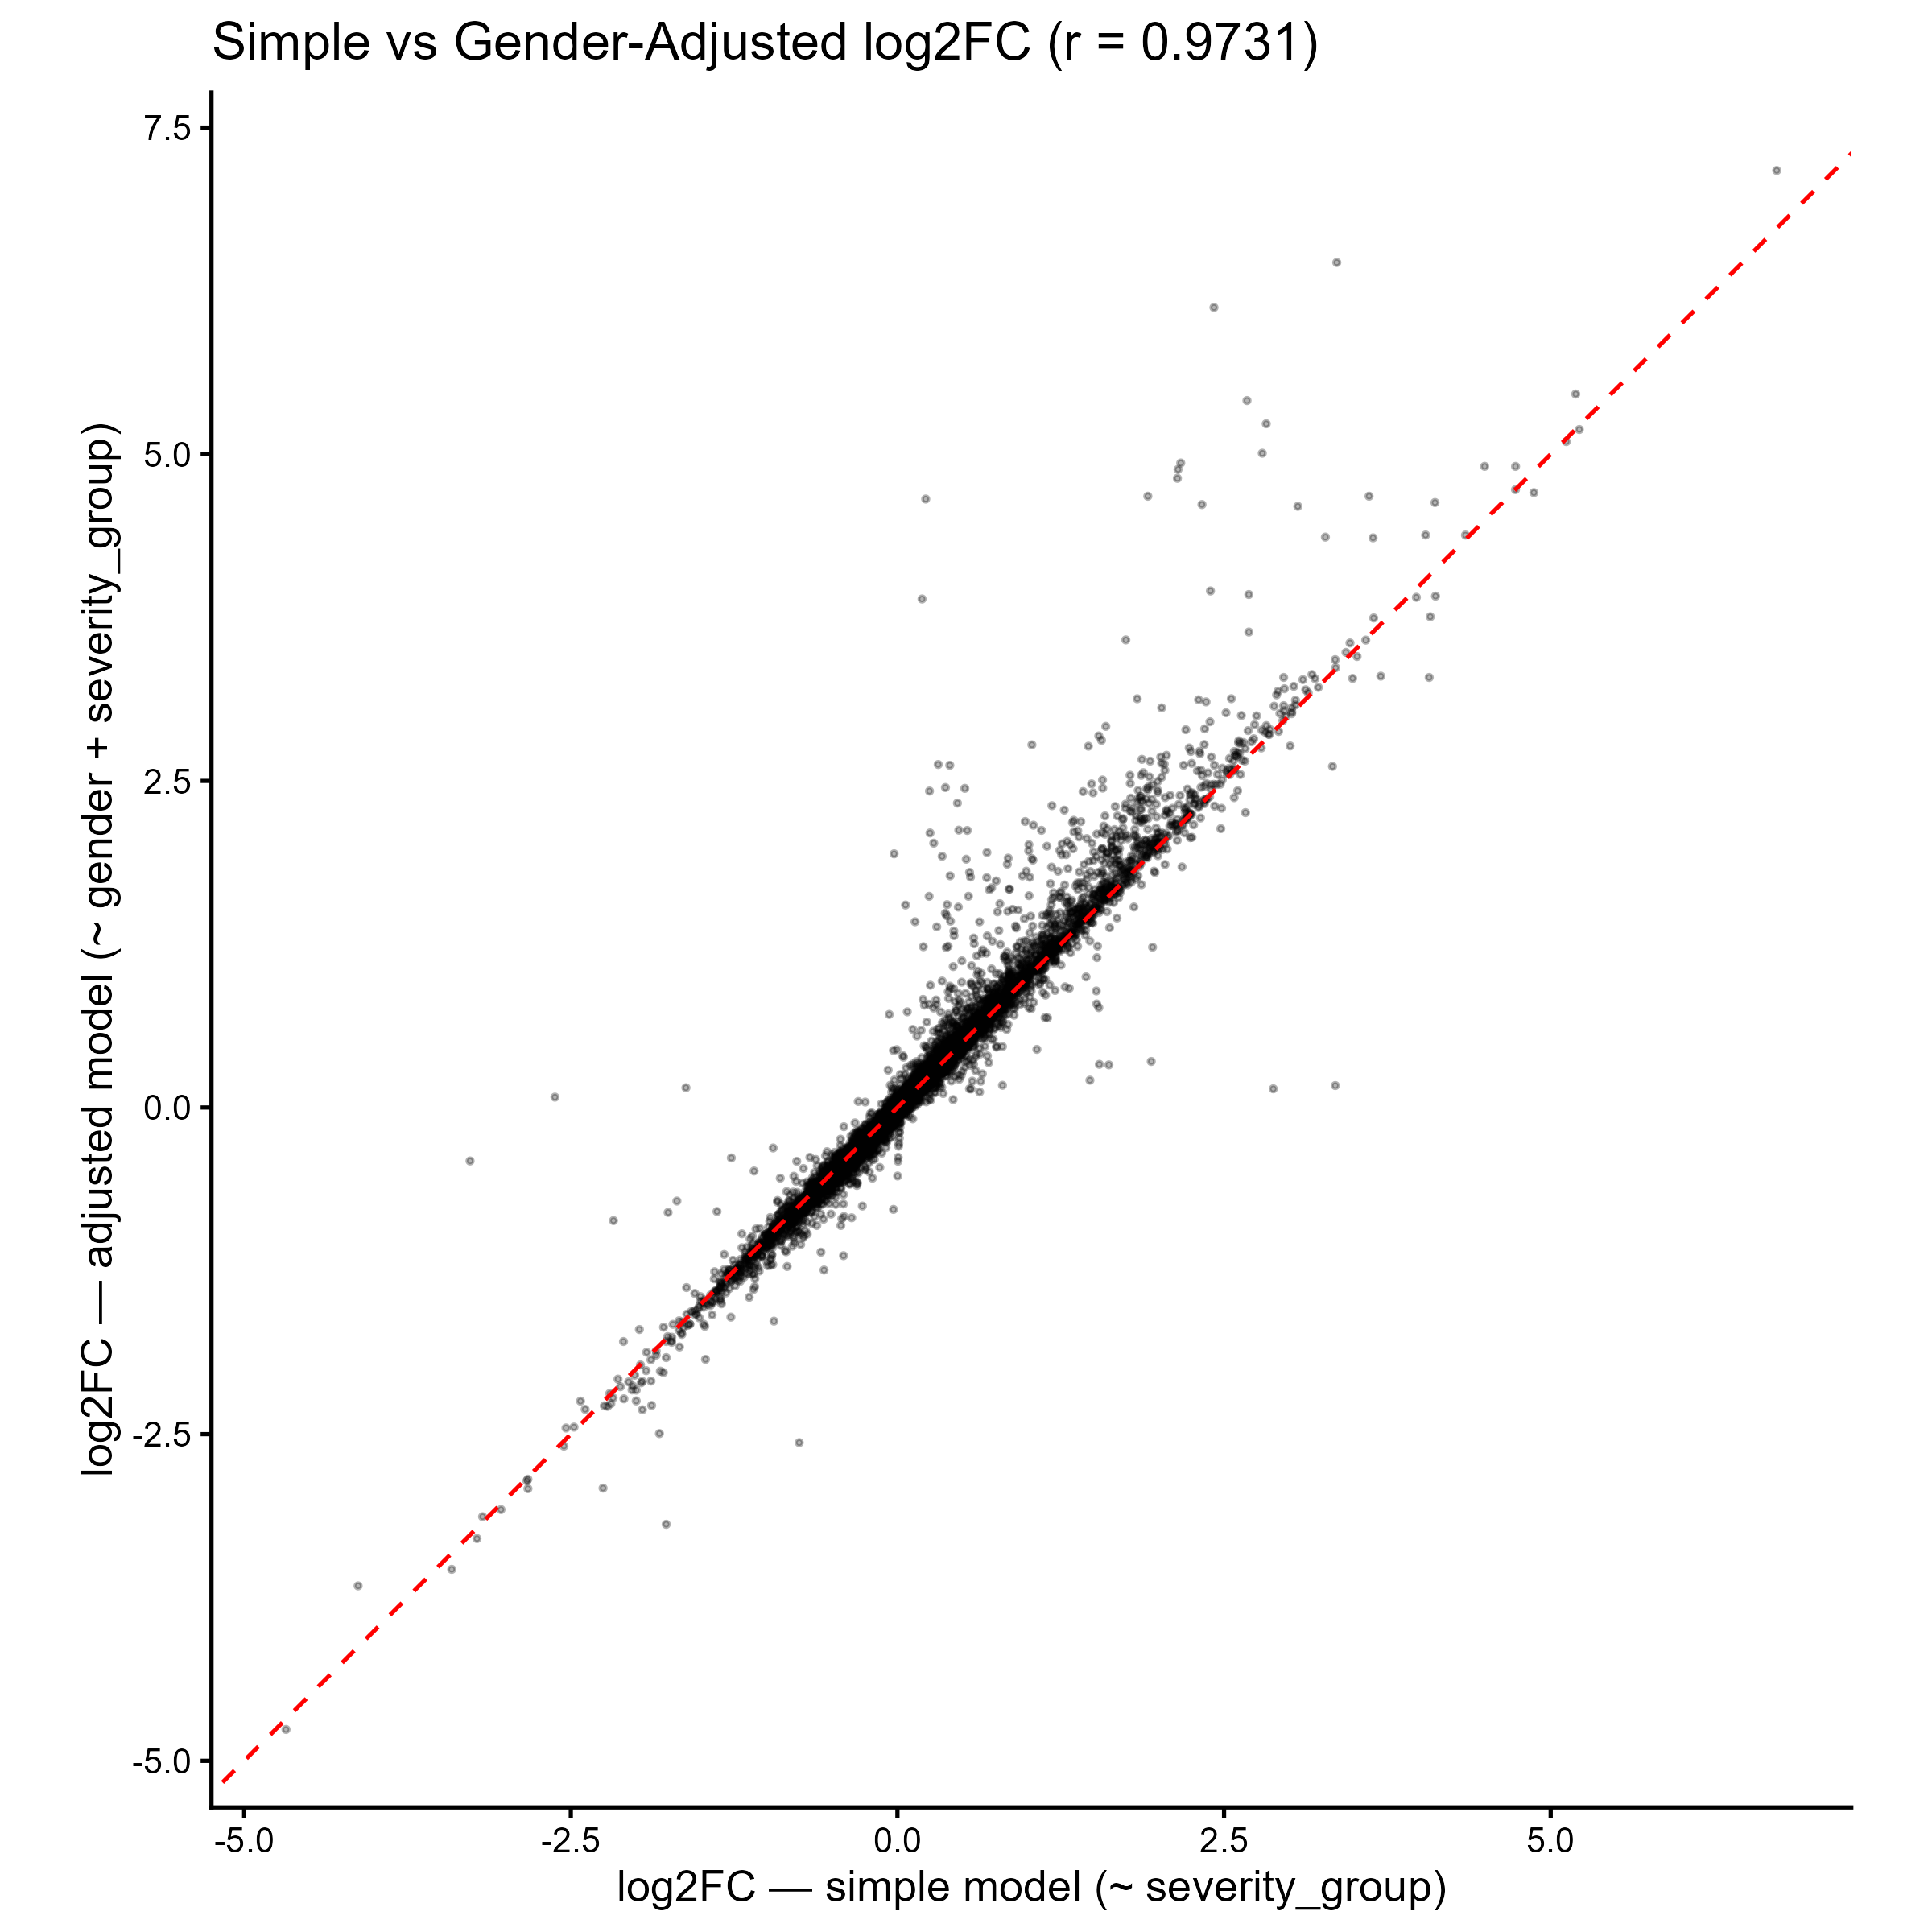
\includegraphics[width=0.85\textwidth]{plots/phase9/phase9_lfc_correlation.png}
\end{center}

Each dot is one gene. The x-axis is its log$_2$ fold-change from the simple
Phase 8 model; the y-axis is its log$_2$ fold-change from the gender-adjusted
model. The red dashed line is the identity line ($y = x$).

\begin{itemize}[nosep]
  \item \textbf{Pearson $r = 0.9731$.} An almost perfect linear correlation.
        The two models agree on the direction and magnitude of change for
        essentially every gene in the dataset.

  \item \textbf{The points hug the diagonal tightly}, with only minor scatter
        around the identity line. A gene that had LFC $= +2$ in Phase 8 has
        LFC $\approx +2$ in Phase 9.

  \item \textbf{A small number of genes deviate from the diagonal} (scatter
        at the edges of the cloud). These are genes whose fold-change was
        partly driven by the gender imbalance — after adjusting for gender,
        their LFC shifts. These genes are \textit{sex-biased} genes that happened
        to correlate with severity in Phase 8. Examples are typically immune
        genes on the X chromosome (e.g.\  \textit{XIST}, \textit{UTY}), or
        genes with known sex-differential expression in blood.

  \item \textbf{The extreme outlier genes (top-right and bottom-left corners)}
        remain at the same LFC in both models — the most significant DE genes
        from Phase 8 (ADAMTS2, S100A12, OLR1, etc.) are real severity effects
        independent of gender.
\end{itemize}

\textbf{Interpretation:} $r = 0.97$ means that 94\% of the variance in
fold-changes is shared between the two models. Gender explains only $\sim$3\%
of the fold-change variance across all genes. The Phase 8 results are robust.

\subsection{Phase 9 conclusion}

Phase 9 was a robustness check, and the answer is clear:
\textbf{gender is not a meaningful confounder for the Phase 8 results.}

\begin{enumerate}[nosep]
  \item \textbf{The gender imbalance was real but mild.}
        Healthy\_Mild is female-majority; Severe\_ICU is male-majority.
        A chi-squared test can detect this imbalance, but the effect on
        gene-level results turns out to be minimal.

  \item \textbf{The MA plots are nearly identical.}
        Adding gender to the model does not remove the bulk of significant
        genes found in Phase 8. The same genes remain significant.

  \item \textbf{Fold-changes are $r = 0.97$ correlated between the two models.}
        This is one of the strongest possible robustness test results —
        the conclusions from Phase 8 hold regardless of whether gender is
        in the model.

  \item \textbf{The adjusted model is used going forward} (Phases 10--13)
        because it is technically more correct: accounting for a known
        covariate is always preferable when it is available, even if
        the practical effect is small. It prevents any future criticism
        that the gender imbalance was ignored.
\end{enumerate}

\textbf{What this means for the story:} the bulk DE results from Phase 8 —
myeloid expansion, platelet activation, lymphocyte depletion — are genuine
disease-severity effects, not artifacts of having more males in the Severe
group. The foundation for Phases 10--13 is solid.

% ─────────────────────────────────────────────
\section{Phase 10 — Bulk RNA-seq Visualization}
% ─────────────────────────────────────────────

\subsection{Phase 10 overview — the big picture}

\textbf{Phases 8 and 9 ran the numbers. Phase 10 makes the story visible.}

At this point we have a list of $\sim$4,000--5,000 DE genes from the
gender-adjusted model. But a table of p-values and fold-changes does not
tell a story. Phase 10 produces four visualizations that do:

\begin{enumerate}[nosep]
  \item \textbf{Volcano plot} — one dot per gene, showing both effect size
        and significance. Lets us read gene names directly.
  \item \textbf{Heatmap of top 50 DE genes} — shows sample-level patterns and
        reveals the role of gender alongside severity.
  \item \textbf{ISG gene boxplots} — tests the hypothesis directly: is the
        antiviral program elevated in severe COVID whole blood?
  \item \textbf{TNF/IL-1$\beta$ gene boxplots} — same for the inflammatory program.
\end{enumerate}

The answer from plots 3 and 4 is the punchline of the bulk chapter:
\textbf{neither program is detectable in bulk whole blood}, even though both were
clearly elevated in monocytes in Phases 4 and 5.
That contrast — cell-level signal invisible at bulk level — is the central
limitation of bulk RNA-seq and the strongest justification for why single-cell
sequencing was necessary in the first place.

\subsection{Volcano plot \small\normalfont\textit{(Step 4)}}

\begin{center}
  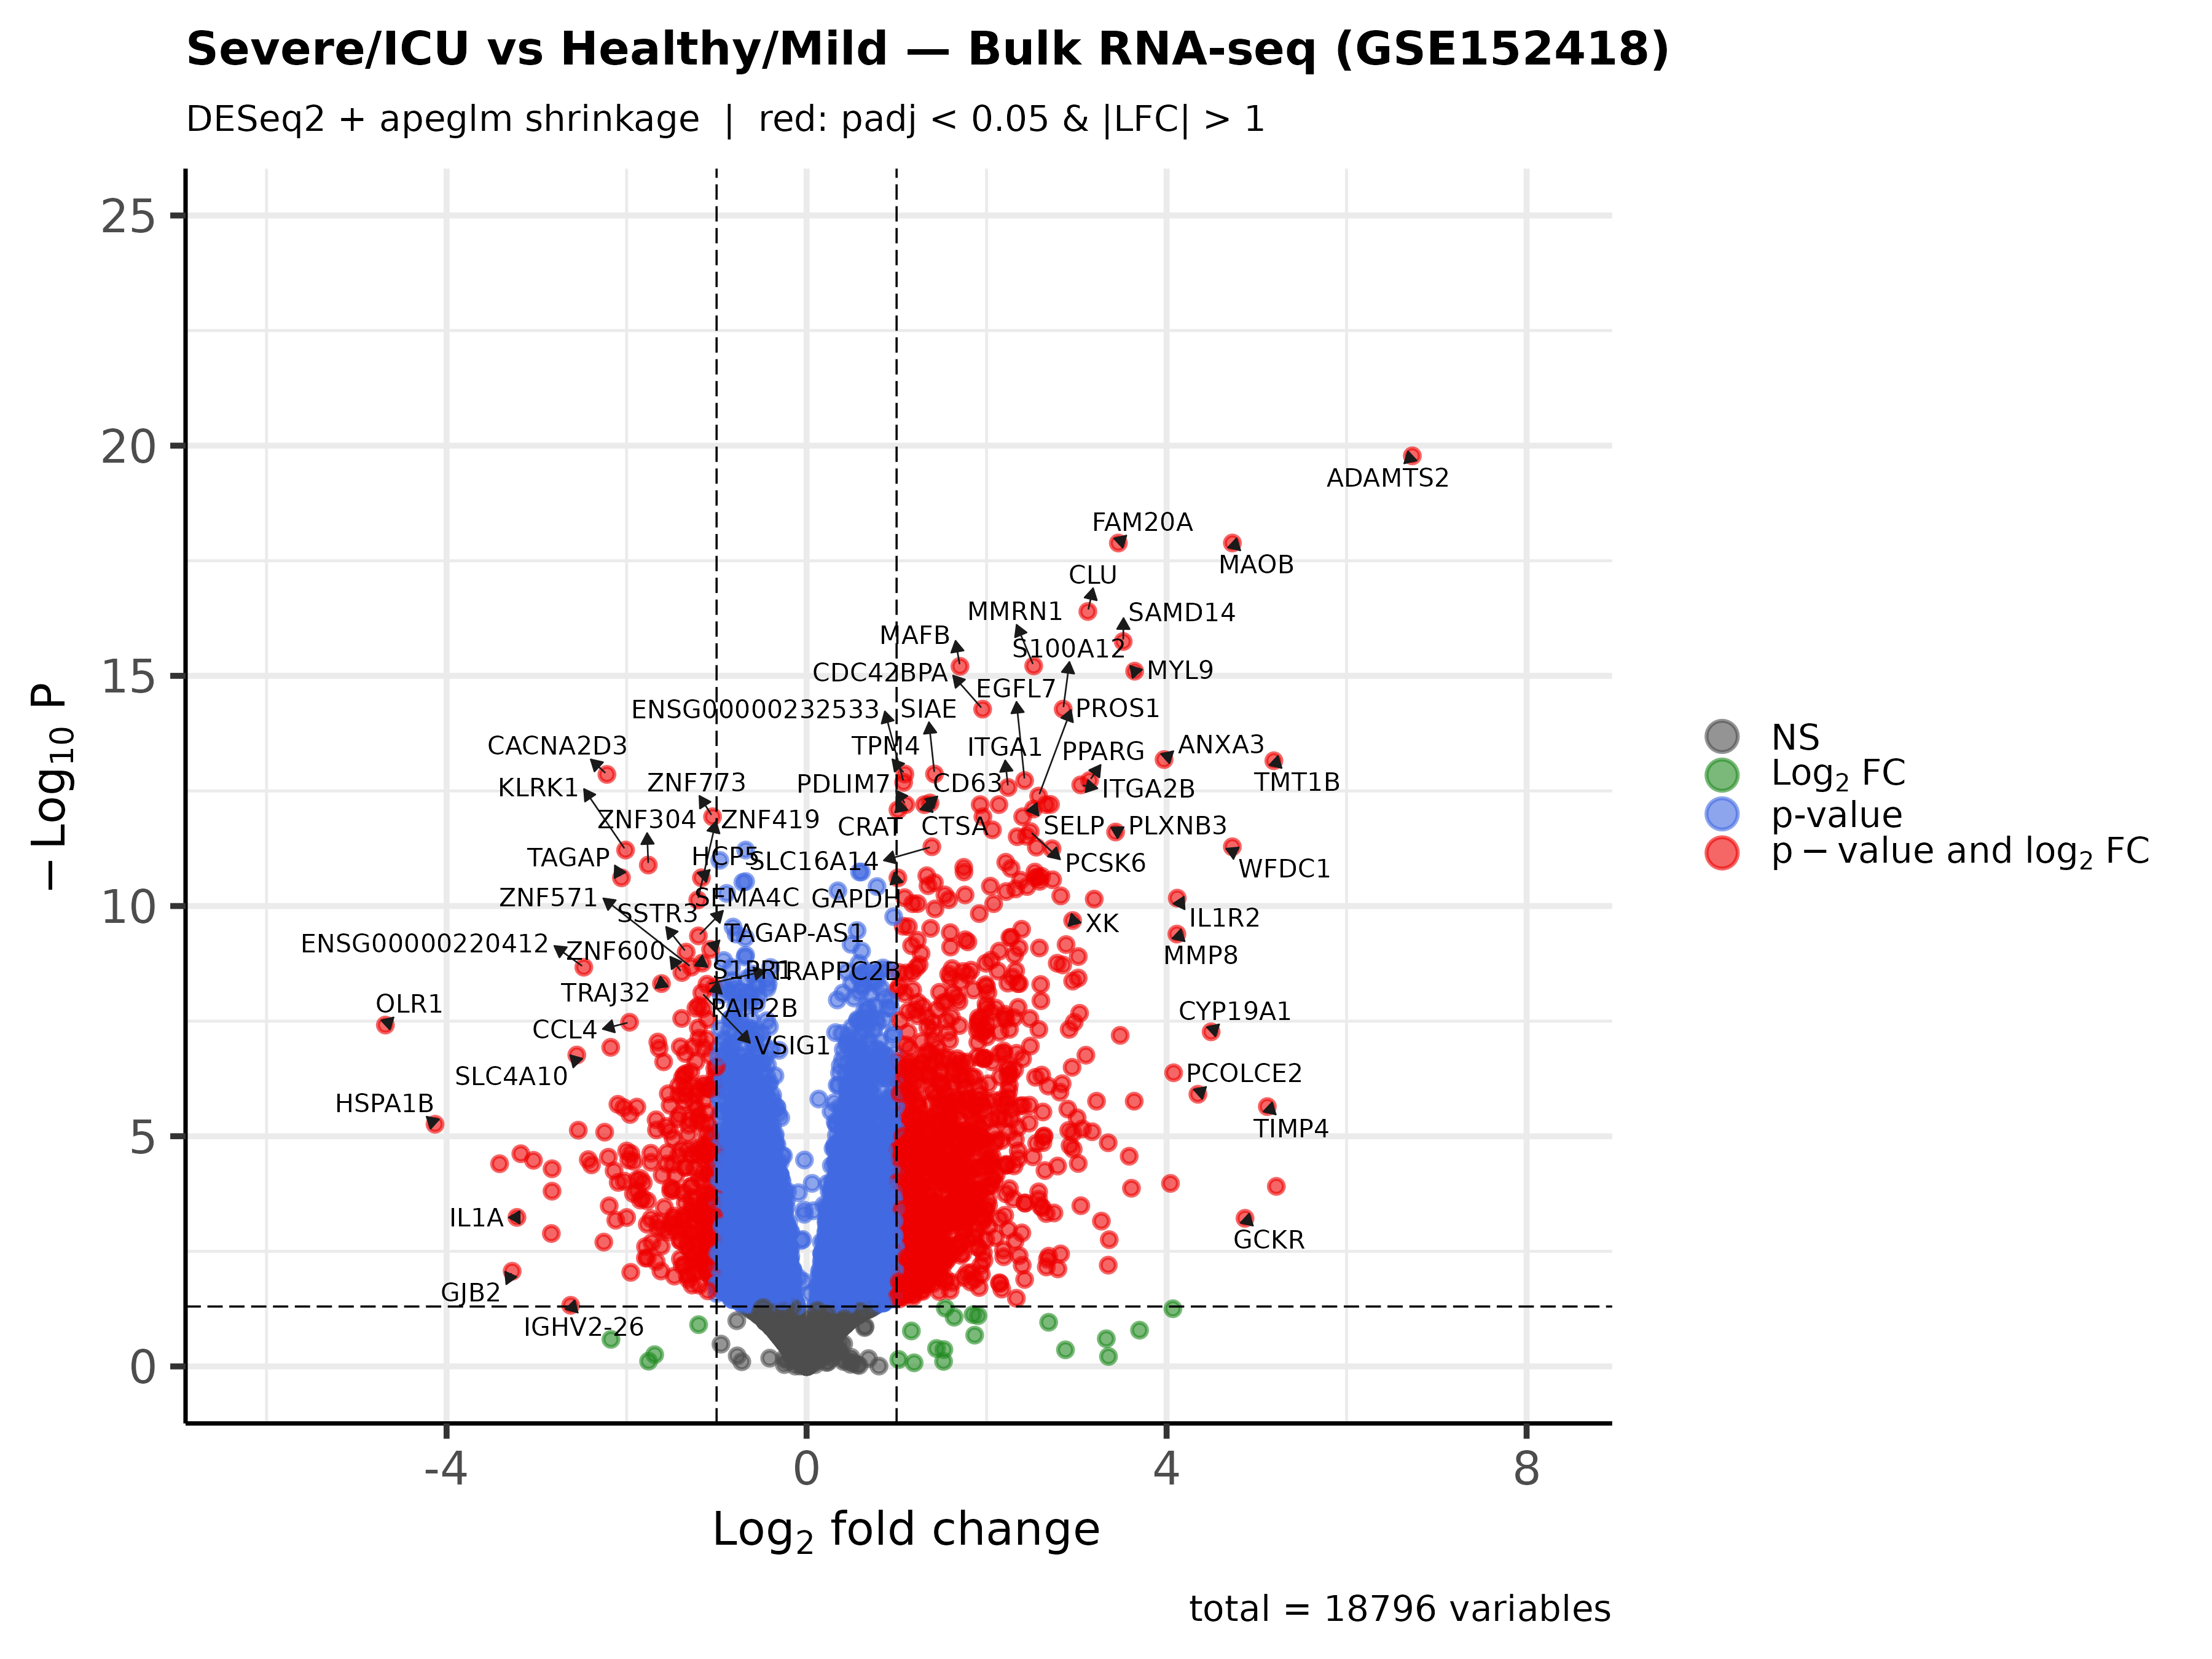
\includegraphics[width=\textwidth]{plots/phase10/phase10_volcano.png}
\end{center}

This is the Phase 8 volcano recreated with the EnhancedVolcano package, which
draws connecting lines from dots to labels so overlapping gene names stay readable.
Each dot is one gene: x-axis = log$_2$ fold-change; y-axis = $-\log_{10}$(adjusted p-value).
\textbf{Red} = significant in both fold-change ($|$LFC$| > 1$) and p-value (padj $< 0.05$).
\textbf{Blue} = significant in p-value only (small fold-change).
\textbf{Grey/green} = not significant.

\textit{Top upregulated genes (top-right, red):}
\begin{itemize}[nosep]
  \item \textbf{ADAMTS2} — the single most extreme result ($-\log_{10}P \approx 21$,
        LFC $\approx +8$). A matrix metalloproteinase produced by activated
        macrophages and monocytes. Its elevation signals tissue remodeling
        driven by the expanded myeloid compartment.
  \item \textbf{FAM20A, CLU, MAOB, MMRN1, SAMD14, S100A12, MYL9} — the next tier
        of significant upregulated genes ($-\log_{10}P \approx 15$--18).
        \textit{MMRN1} and \textit{MYL9} are platelet structural proteins;
        \textit{CLU} (clusterin) is an acute-phase protein from activated myeloid cells;
        \textit{MAOB} is expressed in platelets and monocytes.
        Together they indicate \textbf{platelet activation and myeloid expansion}.
  \item \textbf{MAFB, PPARG} — monocyte-to-macrophage transcription factors.
        Their upregulation confirms that monocytes in severe COVID blood are
        differentiating toward a macrophage-like state.
  \item \textbf{S100A8, S100A9, S100A12} — the S100 alarmin family, produced
        by neutrophils and emergency myeloid progenitors under stress.
  \item \textbf{SELP, ITGA2B, PROS1, F13A1, PPBP} — coagulation and platelet
        activation markers. \textit{SELP} (P-selectin) mediates
        platelet--leukocyte adhesion; \textit{PPBP} is a platelet chemokine.
        The coagulation signal is strong and consistent with the well-known
        thrombotic complications of severe COVID-19.
  \item \textbf{IL1R2} — the decoy IL-1 receptor that blocks IL-1 signaling.
        Its upregulation (rather than IL-1$\beta$ itself) in bulk blood reflects
        the counter-regulatory response: the whole-blood average captures the
        braking mechanism, not the accelerator.
\end{itemize}

\textit{Top downregulated genes (top-left, red):}
\begin{itemize}[nosep]
  \item \textbf{OLR1} — the most significantly downregulated gene
        ($-\log_{10}P \approx 7.5$, LFC $\approx -4.5$). An NK and T cell receptor
        for oxidized LDL. Its loss directly reflects NK cell depletion.
  \item \textbf{KLRK1} (NKG2D) — NK cell activating receptor. Loss = NK depletion.
  \item \textbf{CACNA2D3, ZNF773, ZNF304, ZNF600} — zinc finger transcription
        factors expressed primarily in lymphocytes. Their downregulation tracks
        the loss of the lymphoid compartment.
  \item \textbf{TAGAP, CCL4} — T cell activation GTPase and a T cell chemokine.
        Both lost with T cell depletion.
  \item \textbf{IL1A} — interleukin 1$\alpha$, produced by T cells and monocytes.
        Its downregulation alongside the lymphocyte markers suggests the
        T-cell contribution to IL-1 signaling is lost in bulk severe blood.
  \item \textbf{HSPA1B} — heat shock protein 70 in stressed lymphocytes.
        Lost with lymphocyte depletion.
\end{itemize}

\textbf{Reading both sides together:} the volcano is asymmetric — many more
labeled genes on the upregulated side, and the upregulated genes reach higher
significance scores (up to $-\log_{10}P \approx 21$ vs $\approx 7.5$ on the downside).
This is not because lymphocyte loss is less important — it is because the lymphocyte
markers are more variable across individuals (wide spread in Healthy donors),
reducing their statistical power. The myeloid expansion signal is more consistent
donor-to-donor in severe COVID, making it detectible at higher significance.

\subsection{Heatmap of top 50 DE genes \small\normalfont\textit{(Step 5)}}

\begin{center}
  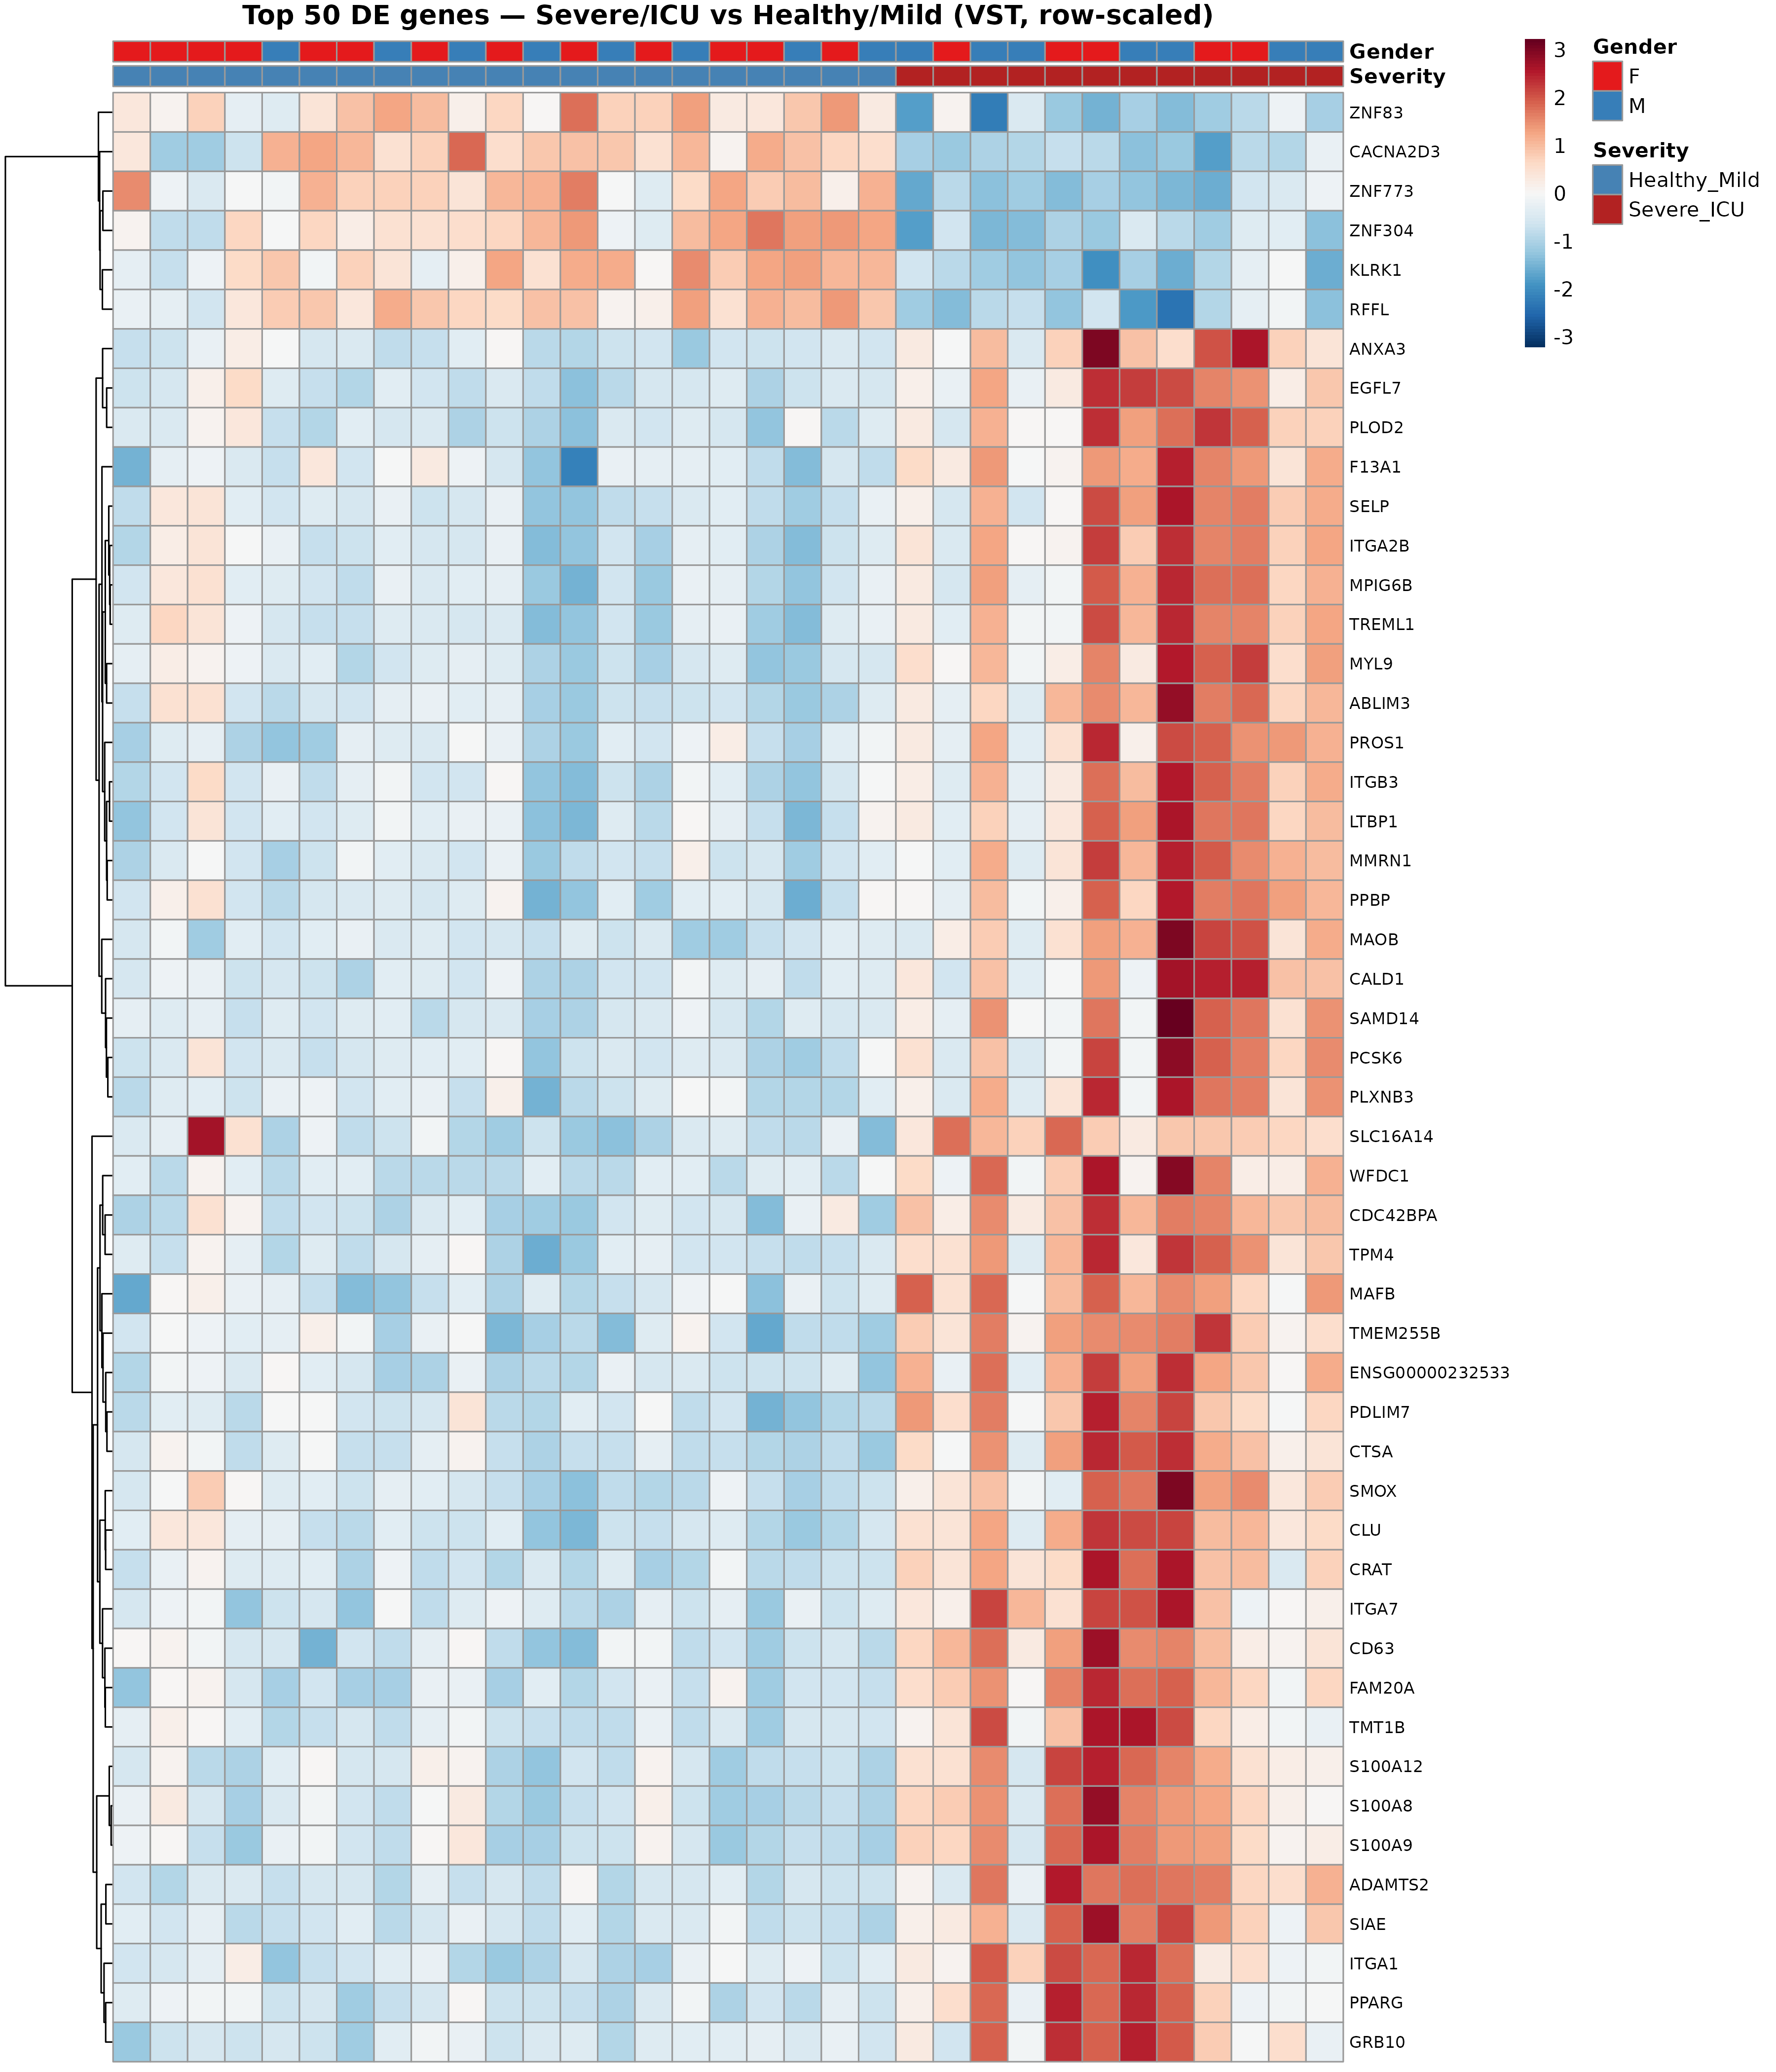
\includegraphics[width=0.95\textwidth]{plots/phase10/phase10_heatmap_top50.png}
\end{center}

The top 50 genes (by adjusted p-value), VST-normalized and row-scaled.
Columns are ordered by severity group (Healthy\_Mild on the left, Severe\_ICU
on the right) — \textit{not} clustered, so the left/right split is the severity split.
Two annotation bars: \textbf{Severity} (blue = Healthy\_Mild, red = Severe\_ICU)
and \textbf{Gender} (salmon = Female, teal = Male).
Row colour: red = high scaled expression; blue = low.

\textit{The two main gene clusters visible in the row dendrogram:}

\begin{itemize}[nosep]
  \item \textbf{Top cluster (downregulated in Severe, $\sim$15 genes):}
        ZNF83, CACNA2D3, ZNF773, ZNF304, KLRK1 — these genes are warm/red in
        the left (Healthy) columns and cool/blue in the right (Severe) columns.
        These are lymphocyte-associated genes lost with T and NK cell depletion.
        The consistent pattern across \textit{all} Severe\_ICU samples (every
        right-side column is blue for these rows) confirms the lymphopenia signal
        is robust and donor-invariant within the Severe group.

  \item \textbf{Middle--bottom cluster (upregulated in Severe, $\sim$35 genes):}
        ADAMTS2, S100A8, S100A9, S100A12, FAM20A, TMT1B, CD63, CLU, MAFB,
        PPARG, MAOB, MMRN1, PPBP, SAMD14, MYL9, ITGA2B, SELP, ANXA3,
        PROS1, CALD1, WFDC1, PCSK6, CDC42BPA, PLXNB3, SIAE, ITGA1 and more.
        These are blue in the left (Healthy) columns and red in the right (Severe).
        The myeloid/platelet upregulation is the dominant and most consistent
        biological signal.
\end{itemize}

\textit{What the Gender bar reveals:}
The Healthy\_Mild group is Female-majority (more salmon) while Severe\_ICU is
Male-majority (more teal), confirming the imbalance from Phase 7.
Importantly, the red/blue pattern in the gene expression rows does not follow
the gender annotation closely — the columns separate cleanly by \textit{Severity},
not by \textit{Gender}. One Healthy\_Mild sample near the boundary shows moderate
upregulation of several Severe-associated genes (a partial ``Severe-like'' pattern)
and happens to be male — consistent with the known trend of more severe outcomes
in males, but this single donor is not enough to drive the group-level results.
The Phase 9 model correction ($r = 0.97$) already quantified that gender explains
very little of the fold-change variance.

\subsection{ISG gene panel (antiviral program) \small\normalfont\textit{(Step 7)}}

\begin{center}
  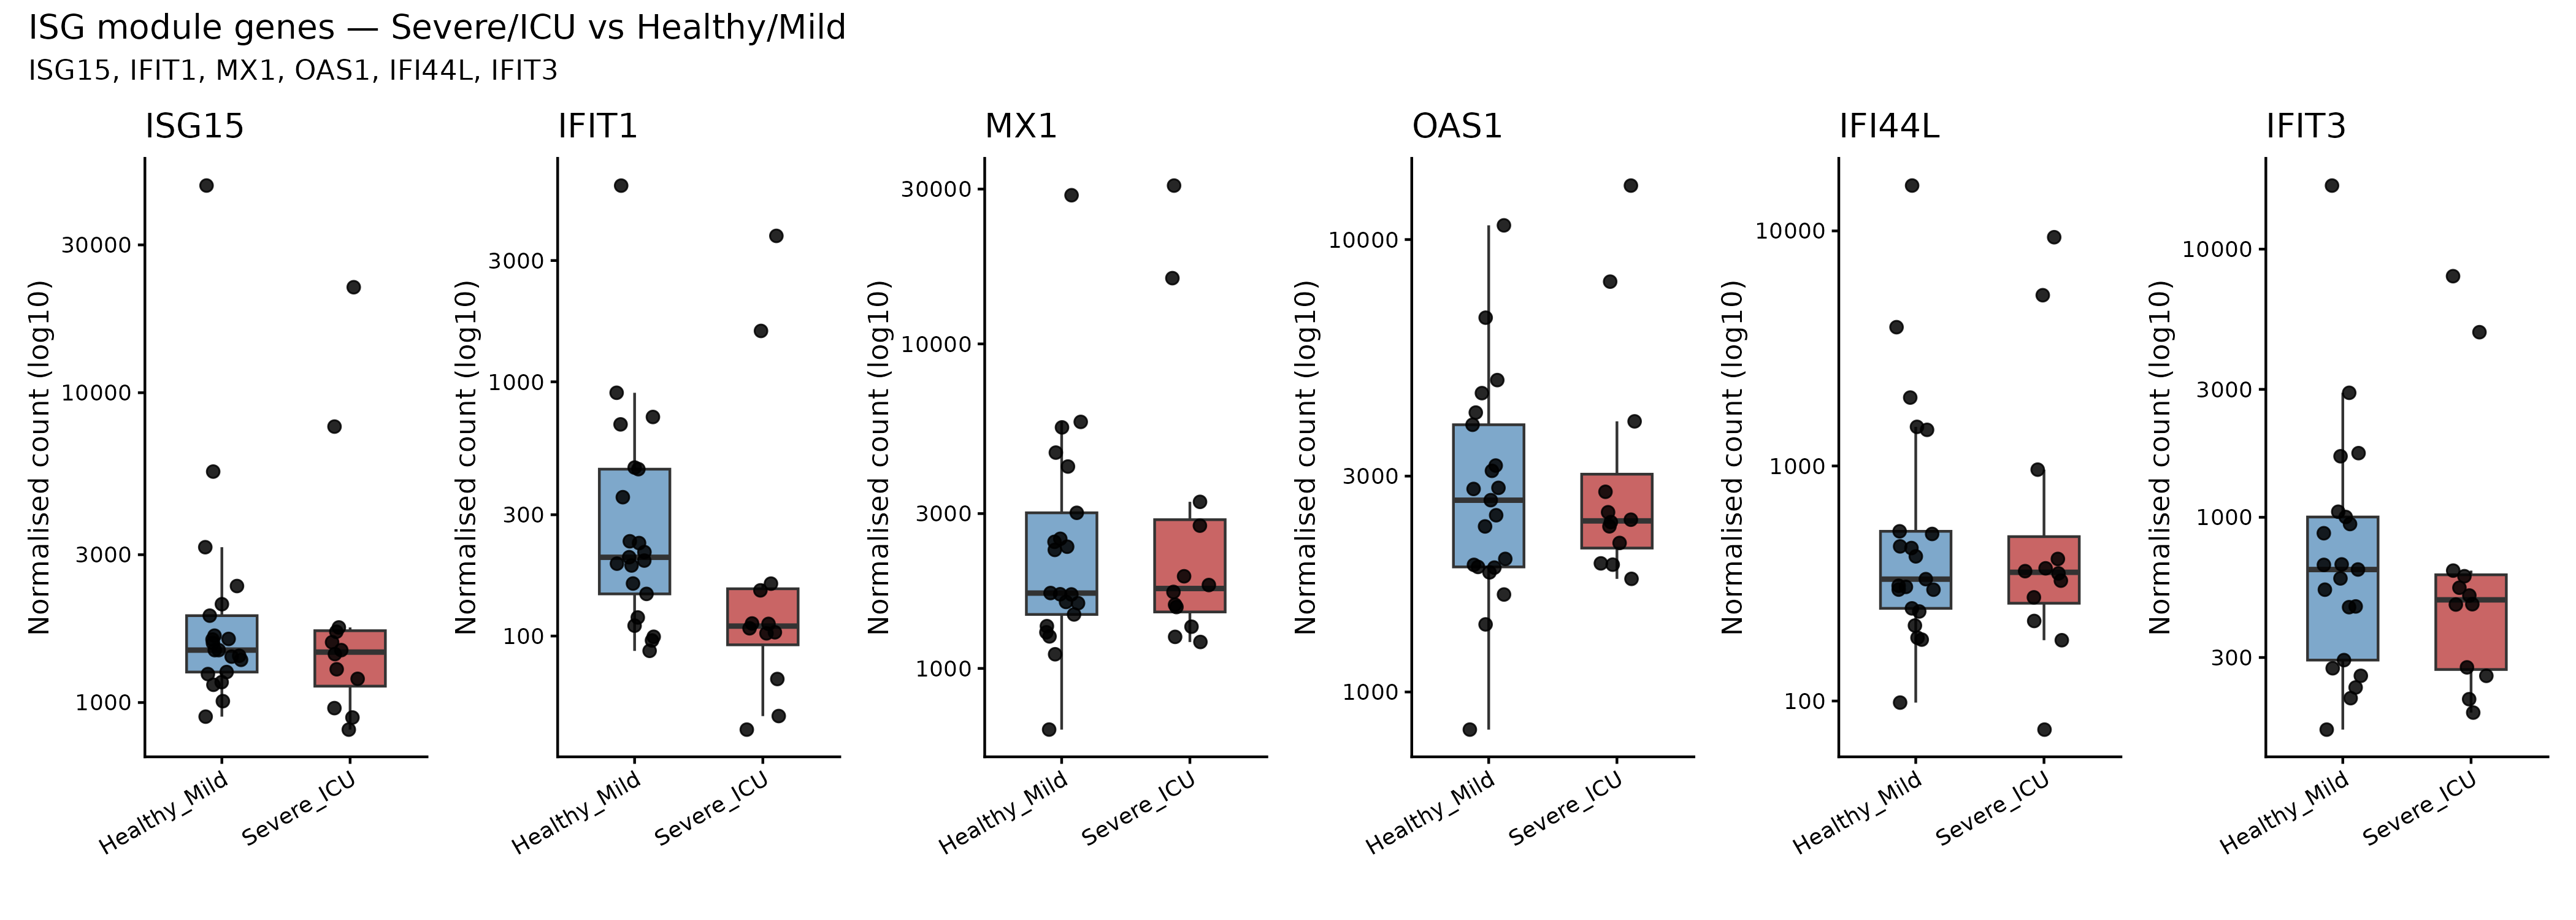
\includegraphics[width=\textwidth]{plots/phase10/phase10_ISG_panel.png}
\end{center}

Six type-I interferon-stimulated genes — ISG15, IFIT1, MX1, OAS1, IFI44L, IFIT3 —
that together define the antiviral module scored in Phase 4. Each boxplot shows
normalised counts (log$_{10}$ scale) in Healthy\_Mild (blue) vs Severe\_ICU (red).
Each dot is one donor.

\begin{itemize}[nosep]
  \item \textbf{ISG15:} Both groups have a median near 1,000--1,500,
        with wide variance. One Healthy\_Mild donor is an extreme outlier at
        $\sim$30,000 — this single donor drives the Healthy group average up.
        There is \textbf{no upward shift in Severe} relative to the main body
        of Healthy donors.
  \item \textbf{IFIT1:} Healthy\_Mild median $\approx$ 200--300;
        Severe\_ICU median $\approx$ 100--150. If anything, \textbf{IFIT1 is
        slightly lower in Severe}. Not elevated.
  \item \textbf{MX1:} Both groups essentially identical ($\sim$2,000--3,000).
        Boxes fully overlap.
  \item \textbf{OAS1:} Similar medians in both groups; slightly wider variance
        in Severe. No directional shift.
  \item \textbf{IFI44L:} Both groups $\approx$ 500--600. Fully overlapping.
  \item \textbf{IFIT3:} Healthy\_Mild slightly higher median.
        Severe\_ICU slightly lower but with large overlap.
\end{itemize}

\textbf{Conclusion:} across all six ISG genes, there is no consistent elevation
in Severe/ICU bulk blood. This six-gene panel extends the three-gene test in
Phase 8 (ISG15, IFIT1, MX1) and returns the same answer. The antiviral program
that was clearly elevated in \textit{monocytes} in Phase 4 is not detectable in
whole blood. The ISG signal is drowned out by the non-ISG-expressing majority of
blood cells.

\subsection{TNF/IL-1$\beta$ gene panel (inflammatory program) \small\normalfont\textit{(Step 7)}}

\begin{center}
  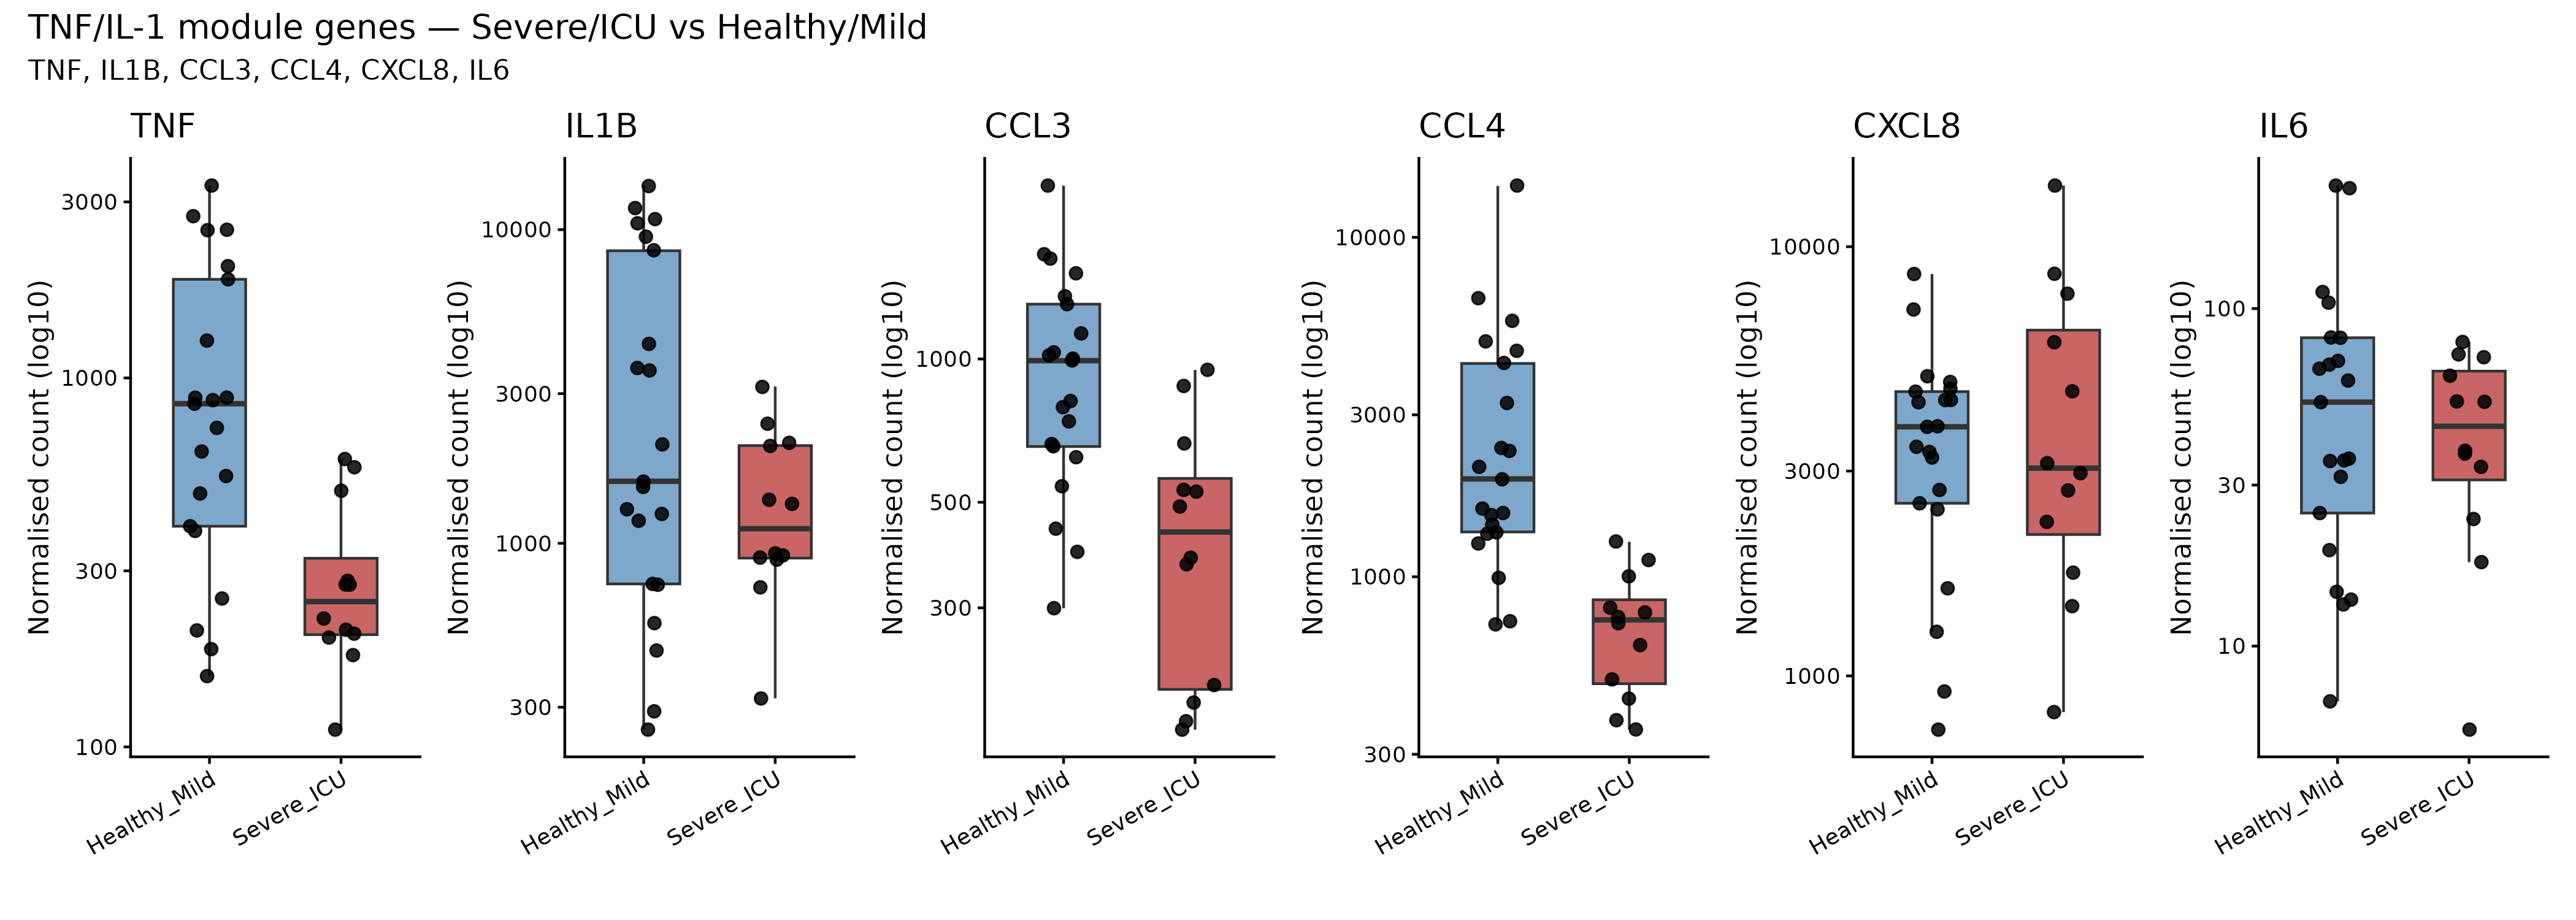
\includegraphics[width=\textwidth]{plots/phase10/phase10_TNF_IL1_panel.png}
\end{center}

Six core inflammatory genes — TNF, IL1B, CCL3, CCL4, CXCL8, IL6 — that define
the monocyte co-activation module.

\begin{itemize}[nosep]
  \item \textbf{TNF:} Healthy\_Mild median $\approx$ 800; Severe\_ICU median
        $\approx$ 280. \textbf{Clearly lower in Severe}. The entire Severe
        box sits below the Healthy lower quartile.
  \item \textbf{IL1B:} Healthy\_Mild median $\approx$ 3,000--5,000;
        Severe\_ICU median $\approx$ 1,500. \textbf{Clearly lower in Severe}.
        Despite being the top upregulated gene in \textit{monocytes} (Phase 4
        volcano, $\log_2$FC $\approx$ 5), it appears \textit{lower} in whole blood.
  \item \textbf{CCL3:} Healthy\_Mild median $\approx$ 1,000; Severe\_ICU median
        $\approx$ 450. Lower in Severe.
  \item \textbf{CCL4:} Healthy\_Mild median $\approx$ 3,000; Severe\_ICU median
        $\approx$ 800. \textbf{Markedly lower} — the most dramatic drop.
  \item \textbf{CXCL8:} Both groups $\approx$ 3,000. Boxes overlap fully.
        A slight upward tendency in Severe (the Severe box extends slightly
        higher), but no clear directional shift.
  \item \textbf{IL6:} Both groups at very low normalized counts ($\sim$30--50),
        roughly equal. IL-6 is produced at low baseline levels in blood even
        during severe disease; it acts as a circulating signal rather than being
        abundant in the blood-cell transcriptome.
\end{itemize}

\textbf{Why are TNF, IL1B, CCL3, and CCL4 \textit{lower} in Severe COVID whole blood?}

This seems paradoxical — Phase 4 showed monocytes producing more IL1B in Severe,
so why is bulk IL1B lower? There are two reasons working together:

\begin{enumerate}[nosep]
  \item \textbf{Lymphocyte depletion.}
        T cells, NK cells, and B cells — all depleted in Severe COVID —
        are steady-state producers of TNF, CCL3, CCL4, and IL1B.
        Their loss from blood removes a large constitutive source of these
        transcripts. This reduction outweighs the gain from monocytes.

  \item \textbf{Monocyte sub-cluster dilution.}
        Only Cluster 7 (IL-1$\beta^+$ monocytes, Phase 3) produces high IL1B.
        That cluster is a minority of all monocytes ($\sim$5--10\% of the
        expanded monocyte compartment). When monocytes are mixed with all other
        blood cell types, the high-IL1B minority is diluted many times over.
\end{enumerate}

These two effects combine to make the net bulk signal \textit{lower in Severe} —
the exact opposite direction from the monocyte-level finding.
This is the core demonstration of why cell-type-resolved single-cell data
was necessary and why bulk RNA-seq cannot answer the original question alone.

\subsection{Phase 10 conclusion}

Phase 10 consolidates the bulk RNA-seq story and directly tests the project hypothesis
against whole-blood data. The key findings:

\begin{enumerate}[nosep]
  \item \textbf{The dominant bulk signal is myeloid/platelet expansion and
        lymphocyte loss.}
        ADAMTS2, S100A8/9/12, MAFB, platelet structural proteins, and
        coagulation factors are the top upregulated genes. OLR1, KLRK1,
        lymphocyte zinc-finger factors, and T cell chemokines are the
        top downregulated genes. This is the cell-composition shift,
        not the cell-intrinsic biology.

  \item \textbf{The ISG program (6 genes) is not elevated in bulk blood.}
        No ISG gene shows a consistent upward shift in Severe/ICU compared
        to Healthy/Mild. In fact, several are slightly lower.

  \item \textbf{The TNF/IL-1$\beta$ program (6 genes) is lower in bulk blood.}
        TNF, IL1B, CCL3, CCL4 are all clearly lower in Severe/ICU.
        The monocyte-level upregulation is overwhelmed by lymphocyte depletion
        and monocyte sub-cluster dilution.

  \item \textbf{The heatmap confirms that the top 50 genes perfectly separate
        severity groups using only 50 genes.}
        But what separates them is the composition shift — not the co-activation
        biology discovered in Phase 4.

  \item \textbf{The Phase 9 robustness finding (gender barely matters, $r = 0.97$)
        holds across all visualizations.}
        No plot shows a pattern clearly driven by gender rather than severity.
\end{enumerate}

\textbf{What this means for the overall story:}
The single-cell chapter (Phases 3--6) and the bulk chapter (Phases 7--10)
are telling the same story from two different altitudes.
From high altitude (bulk), you see armies moving: monocytes flooding in,
lymphocytes retreating. From cell level (single-cell), you see individual
soldiers: a subset of monocytes running both the antiviral and inflammatory
programs at the same time. Both views are real. But only the cell-level
view can answer whether the co-activated state exists.

% ─────────────────────────────────────────────────────────
\subsection{VST normalization — making samples comparable for clustering}

Before running PCA or distance-based clustering on bulk samples, raw counts must
be transformed so that variance is stable across the expression range.

\textbf{VST (variance-stabilizing transformation)} corrects the fact that
high-count genes have much larger raw variances than low-count genes
(the mean-variance dependency confirmed in Phase 8). After VST, each gene
contributes roughly equally to distances and PCA regardless of its baseline count.

Setting \texttt{blind = TRUE} means the transformation ignores the experiment
groupings — it is computed as if all samples came from the same population.
This is the correct choice for \textbf{unsupervised} analysis: we want the
data to reveal its own structure, not the structure we already know.

% ─────────────────────────────────────────────
\section{Phase 11 — PCA and Clustering of Bulk Samples}
% ─────────────────────────────────────────────

\subsection{Phase 11 overview — the big picture}

\textbf{Phases 8--10 tested individual genes. Phase 11 asks: do the samples
themselves cluster by severity without being told their labels?}

In Phases 8--10 we asked gene-by-gene which ones change between groups.
That is a bottom-up view — start from individual genes and build up to biology.
Phase 11 takes the opposite, top-down view: forget individual genes for a moment.
If you take the 1,000 most variable genes together, do the samples naturally
fall into two groups that match Healthy/Mild vs Severe/ICU — on their own?

This is called \textbf{unsupervised analysis}: no labels are given to the algorithm.
If samples still separate by severity, it means the disease difference is so
pervasive across the transcriptome that it organises samples by itself.
That would validate all the gene-level findings from Phases 8--10.

Three independent methods are applied to the same VST-normalized top-1,000 genes:
\begin{enumerate}[nosep]
  \item \textbf{PCA} — project samples into 2D space and colour by severity.
  \item \textbf{Correlation and distance matrices} — measure how similar every pair
        of samples is.
  \item \textbf{Hierarchical clustering and k-means} — let two different algorithms
        group samples with no label input.
\end{enumerate}

If all three agree, the severity split is a robust structure in the data, not a
statistical artefact.

\subsection{PCA \small\normalfont\textit{(Steps 5a--5e)}}

\textit{Note: here PCA is applied to \textbf{samples}, not genes. Each sample is
described by its expression across 1,000 genes, and PCA finds the main axes of
variation between samples. This is the transpose of scRNA-seq PCA, where each
individual cell was a point.}

\subsubsection*{Step 5b — Scree plot}

\begin{center}
  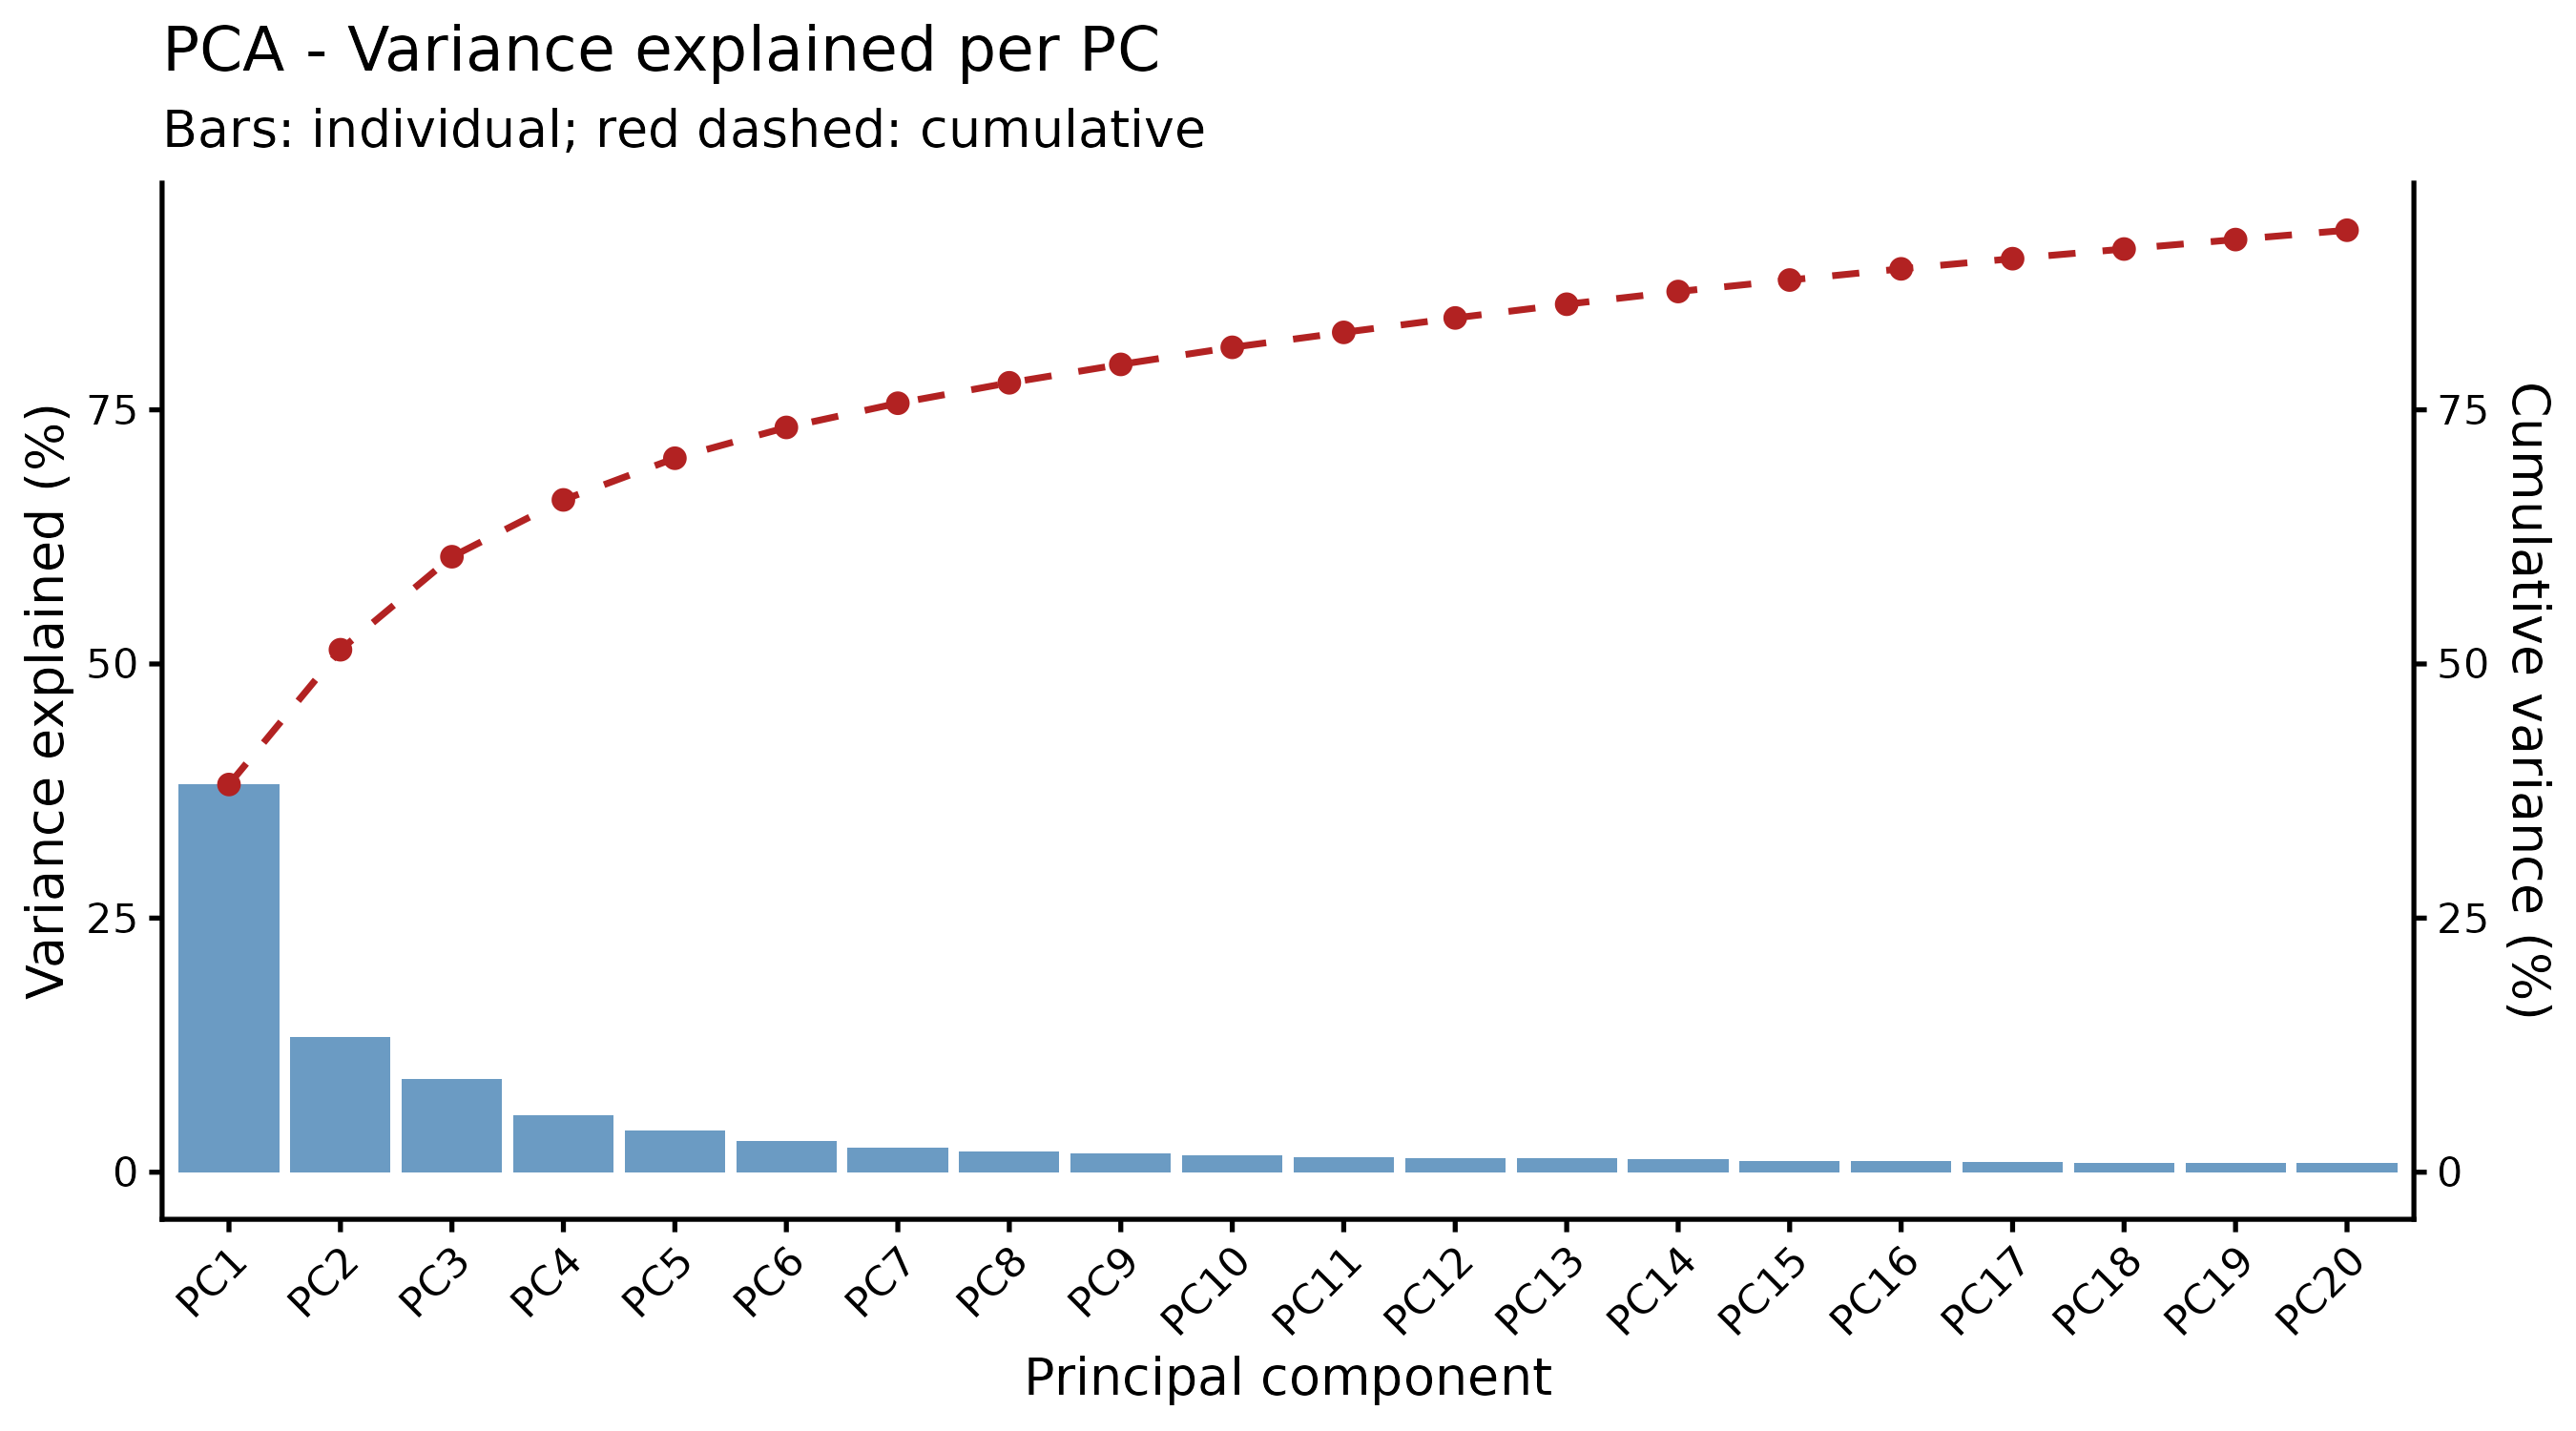
\includegraphics[width=0.9\textwidth]{plots/phase11/phase11_PCA_scree.png}
\end{center}

\begin{itemize}[nosep]
  \item \textbf{PC1 explains 38.14\%} of all sample-to-sample variance — a dominant
        single axis. In a dataset with no clear group structure, PC1 would explain
        far less. Nearly 40\% in one component strongly hints that one large signal
        drives the data.
  \item \textbf{PC2 explains 13.26\%}; PC3 = 9.15\%; PC4 $\approx$6\%; PC5 $\approx$4.5\%.
  \item After PC5, the curve flattens to a slow linear decay — the noise floor.
  \item Cumulative variance: PC1+PC2 $\approx$51\%; top 5 PCs $\approx$71\%;
        top 10 PCs $\approx$80\%.
  \item \textbf{Conclusion:} most informative variance lives in the first 5 PCs, and
        PC1 alone captures more than a third. PC1 is the prime candidate for a severity
        axis.
\end{itemize}

\subsubsection*{Step 5c — PCA coloured by severity}

\begin{center}
  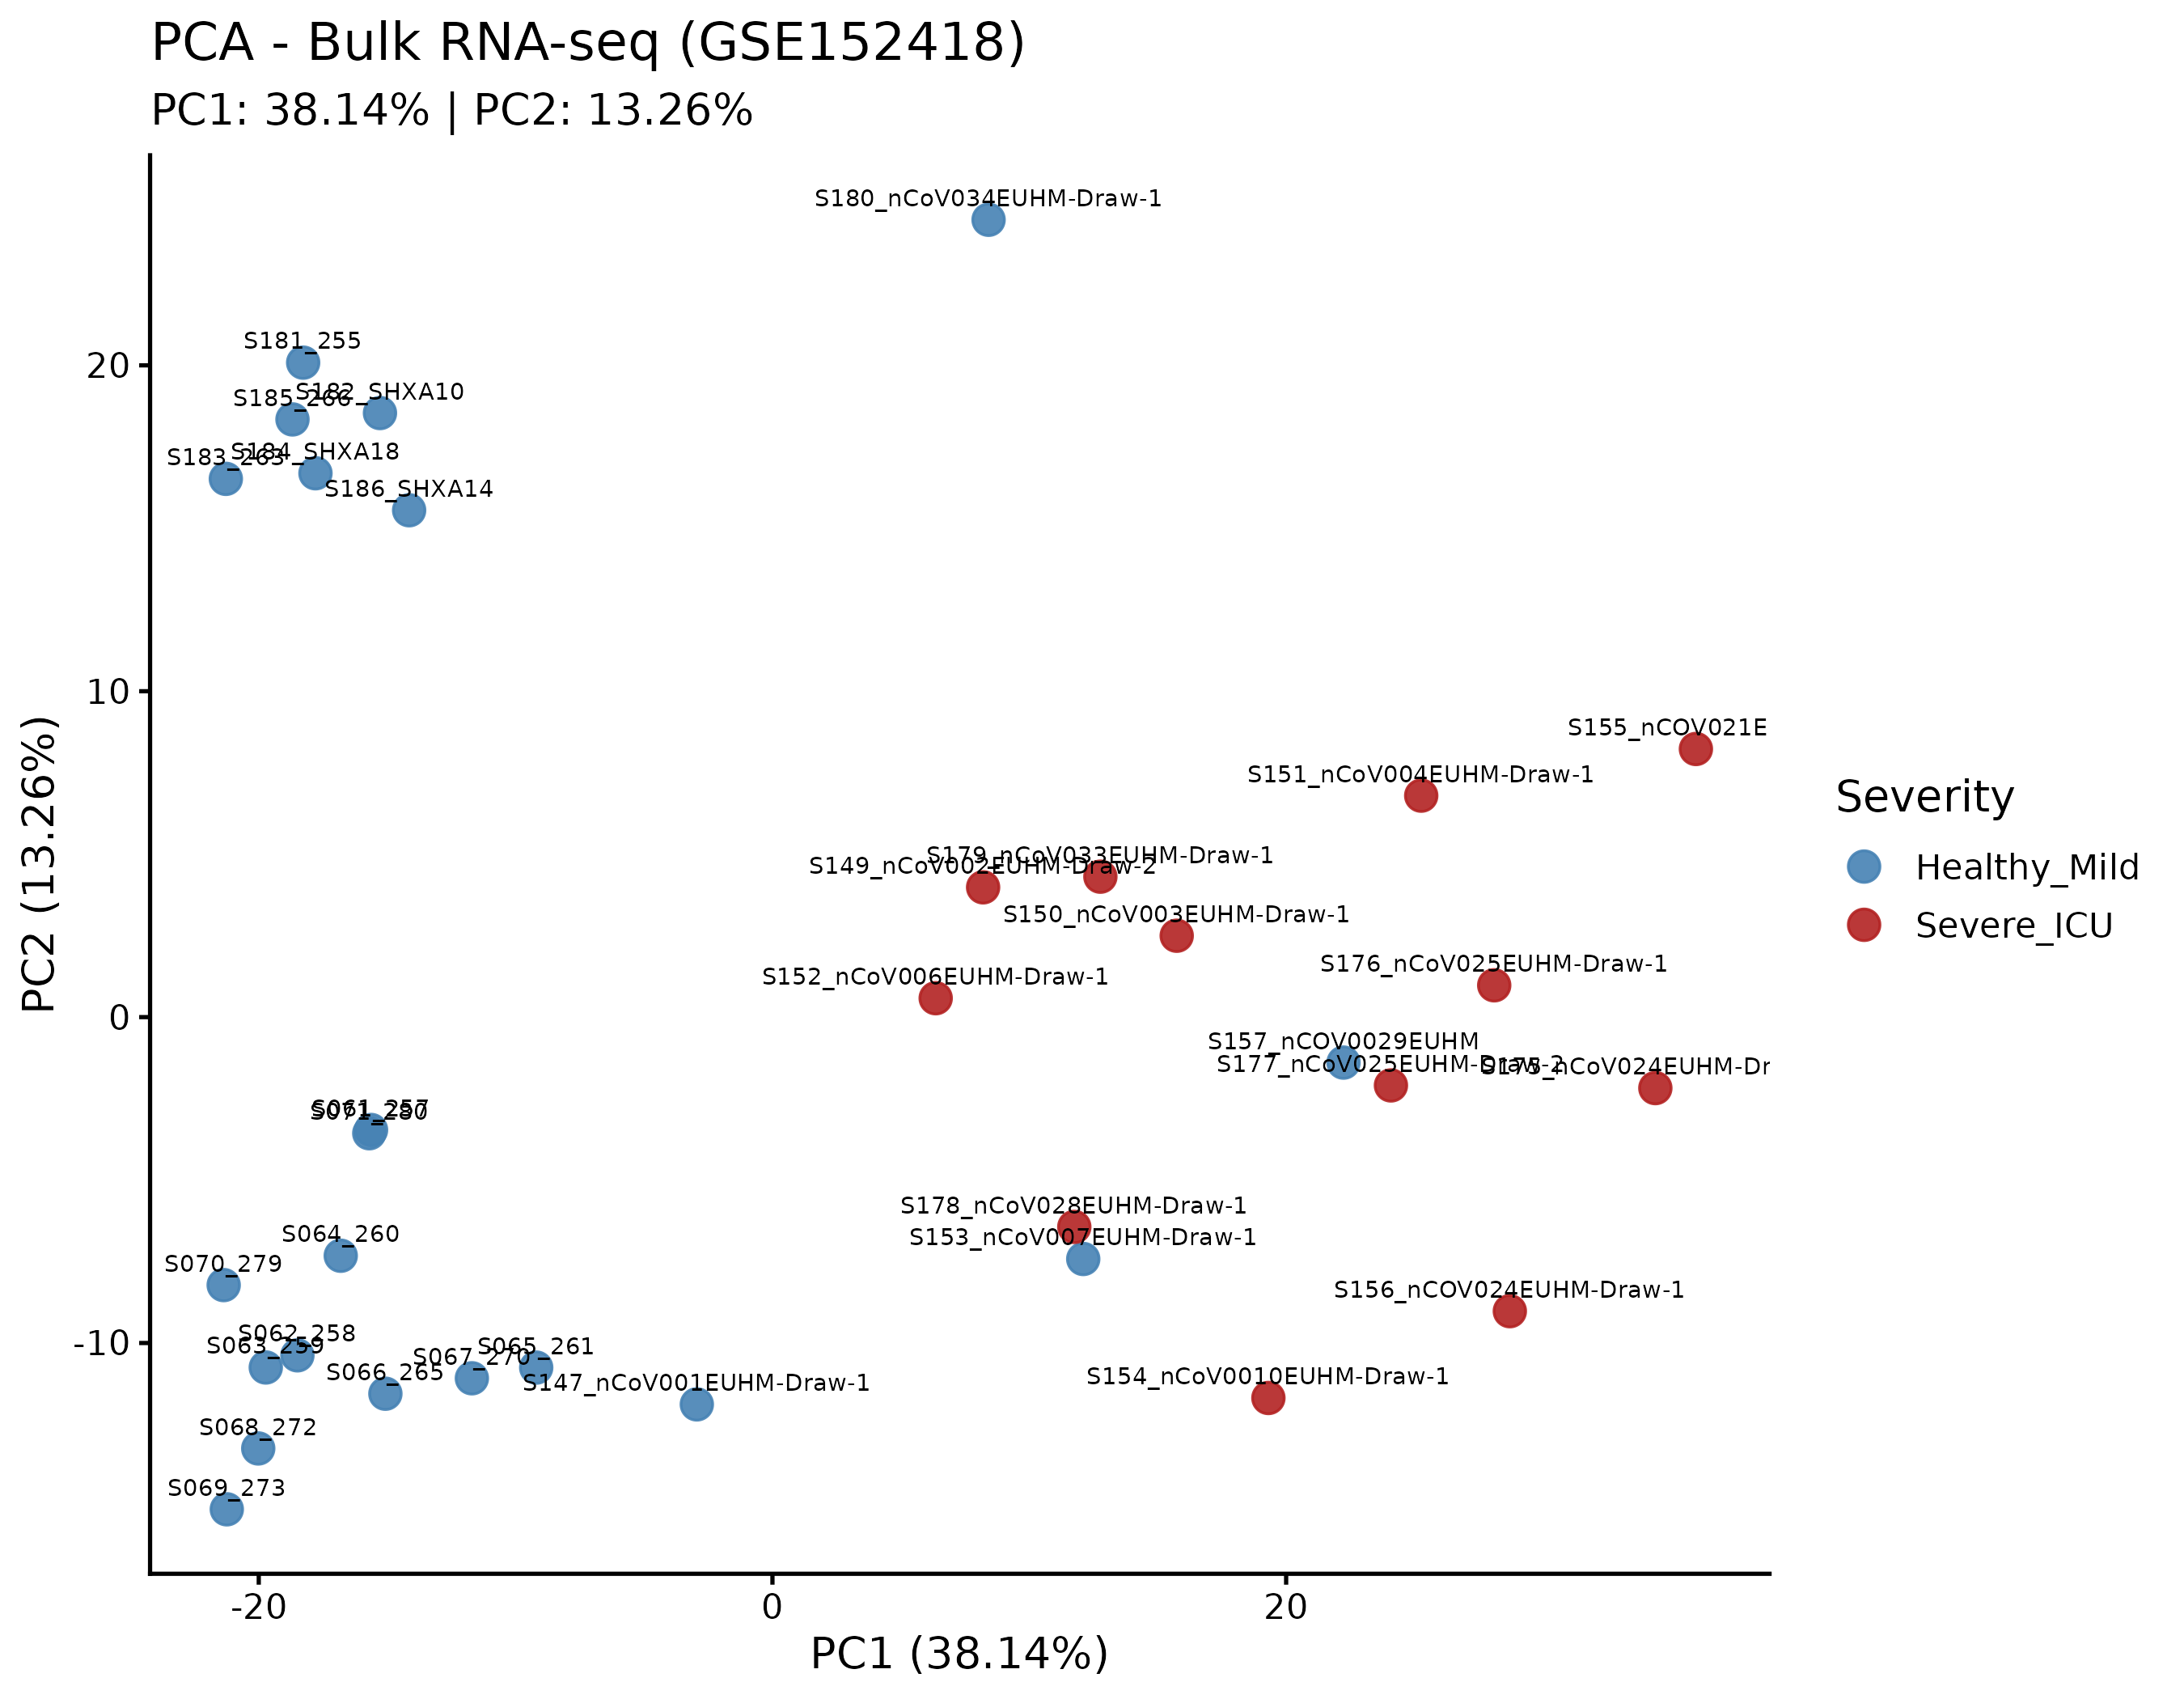
\includegraphics[width=0.9\textwidth]{plots/phase11/phase11_PCA_severity.png}
\end{center}

\begin{itemize}[nosep]
  \item \textbf{PC1 perfectly separates the two groups.} All Healthy/Mild samples
        (blue) sit at negative PC1 ($\approx -25$ to $-10$); all Severe/ICU samples
        (red) sit at positive PC1 ($\approx 0$ to $+25$). There is a clear gap around
        PC1 = 0 with no overlap.
  \item \textbf{PC2 does not separate groups.} Both blue and red samples spread
        across the full PC2 range ($-15$ to $+25$). PC2 captures within-condition
        donor-to-donor variability, not disease severity.
  \item \textbf{One Severe outlier:} S180\_nCoV034EUHM-Draw-1 sits considerably
        higher on PC2 ($\approx+25$) than all other Severe samples. It is still on the
        correct (positive) side of PC1. This donor likely has an unusually strong
        secondary biological signal unrelated to the main severity difference.
  \item The \textbf{Severe cluster is wider} on PC1 than the Healthy cluster —
        Severe/ICU donors are more variable in their transcriptomes from each other
        than Healthy/Mild donors. Each patient's immune crisis unfolds differently.
\end{itemize}

\subsubsection*{Step 5d — PCA coloured by severity, shaped by gender}

\begin{center}
  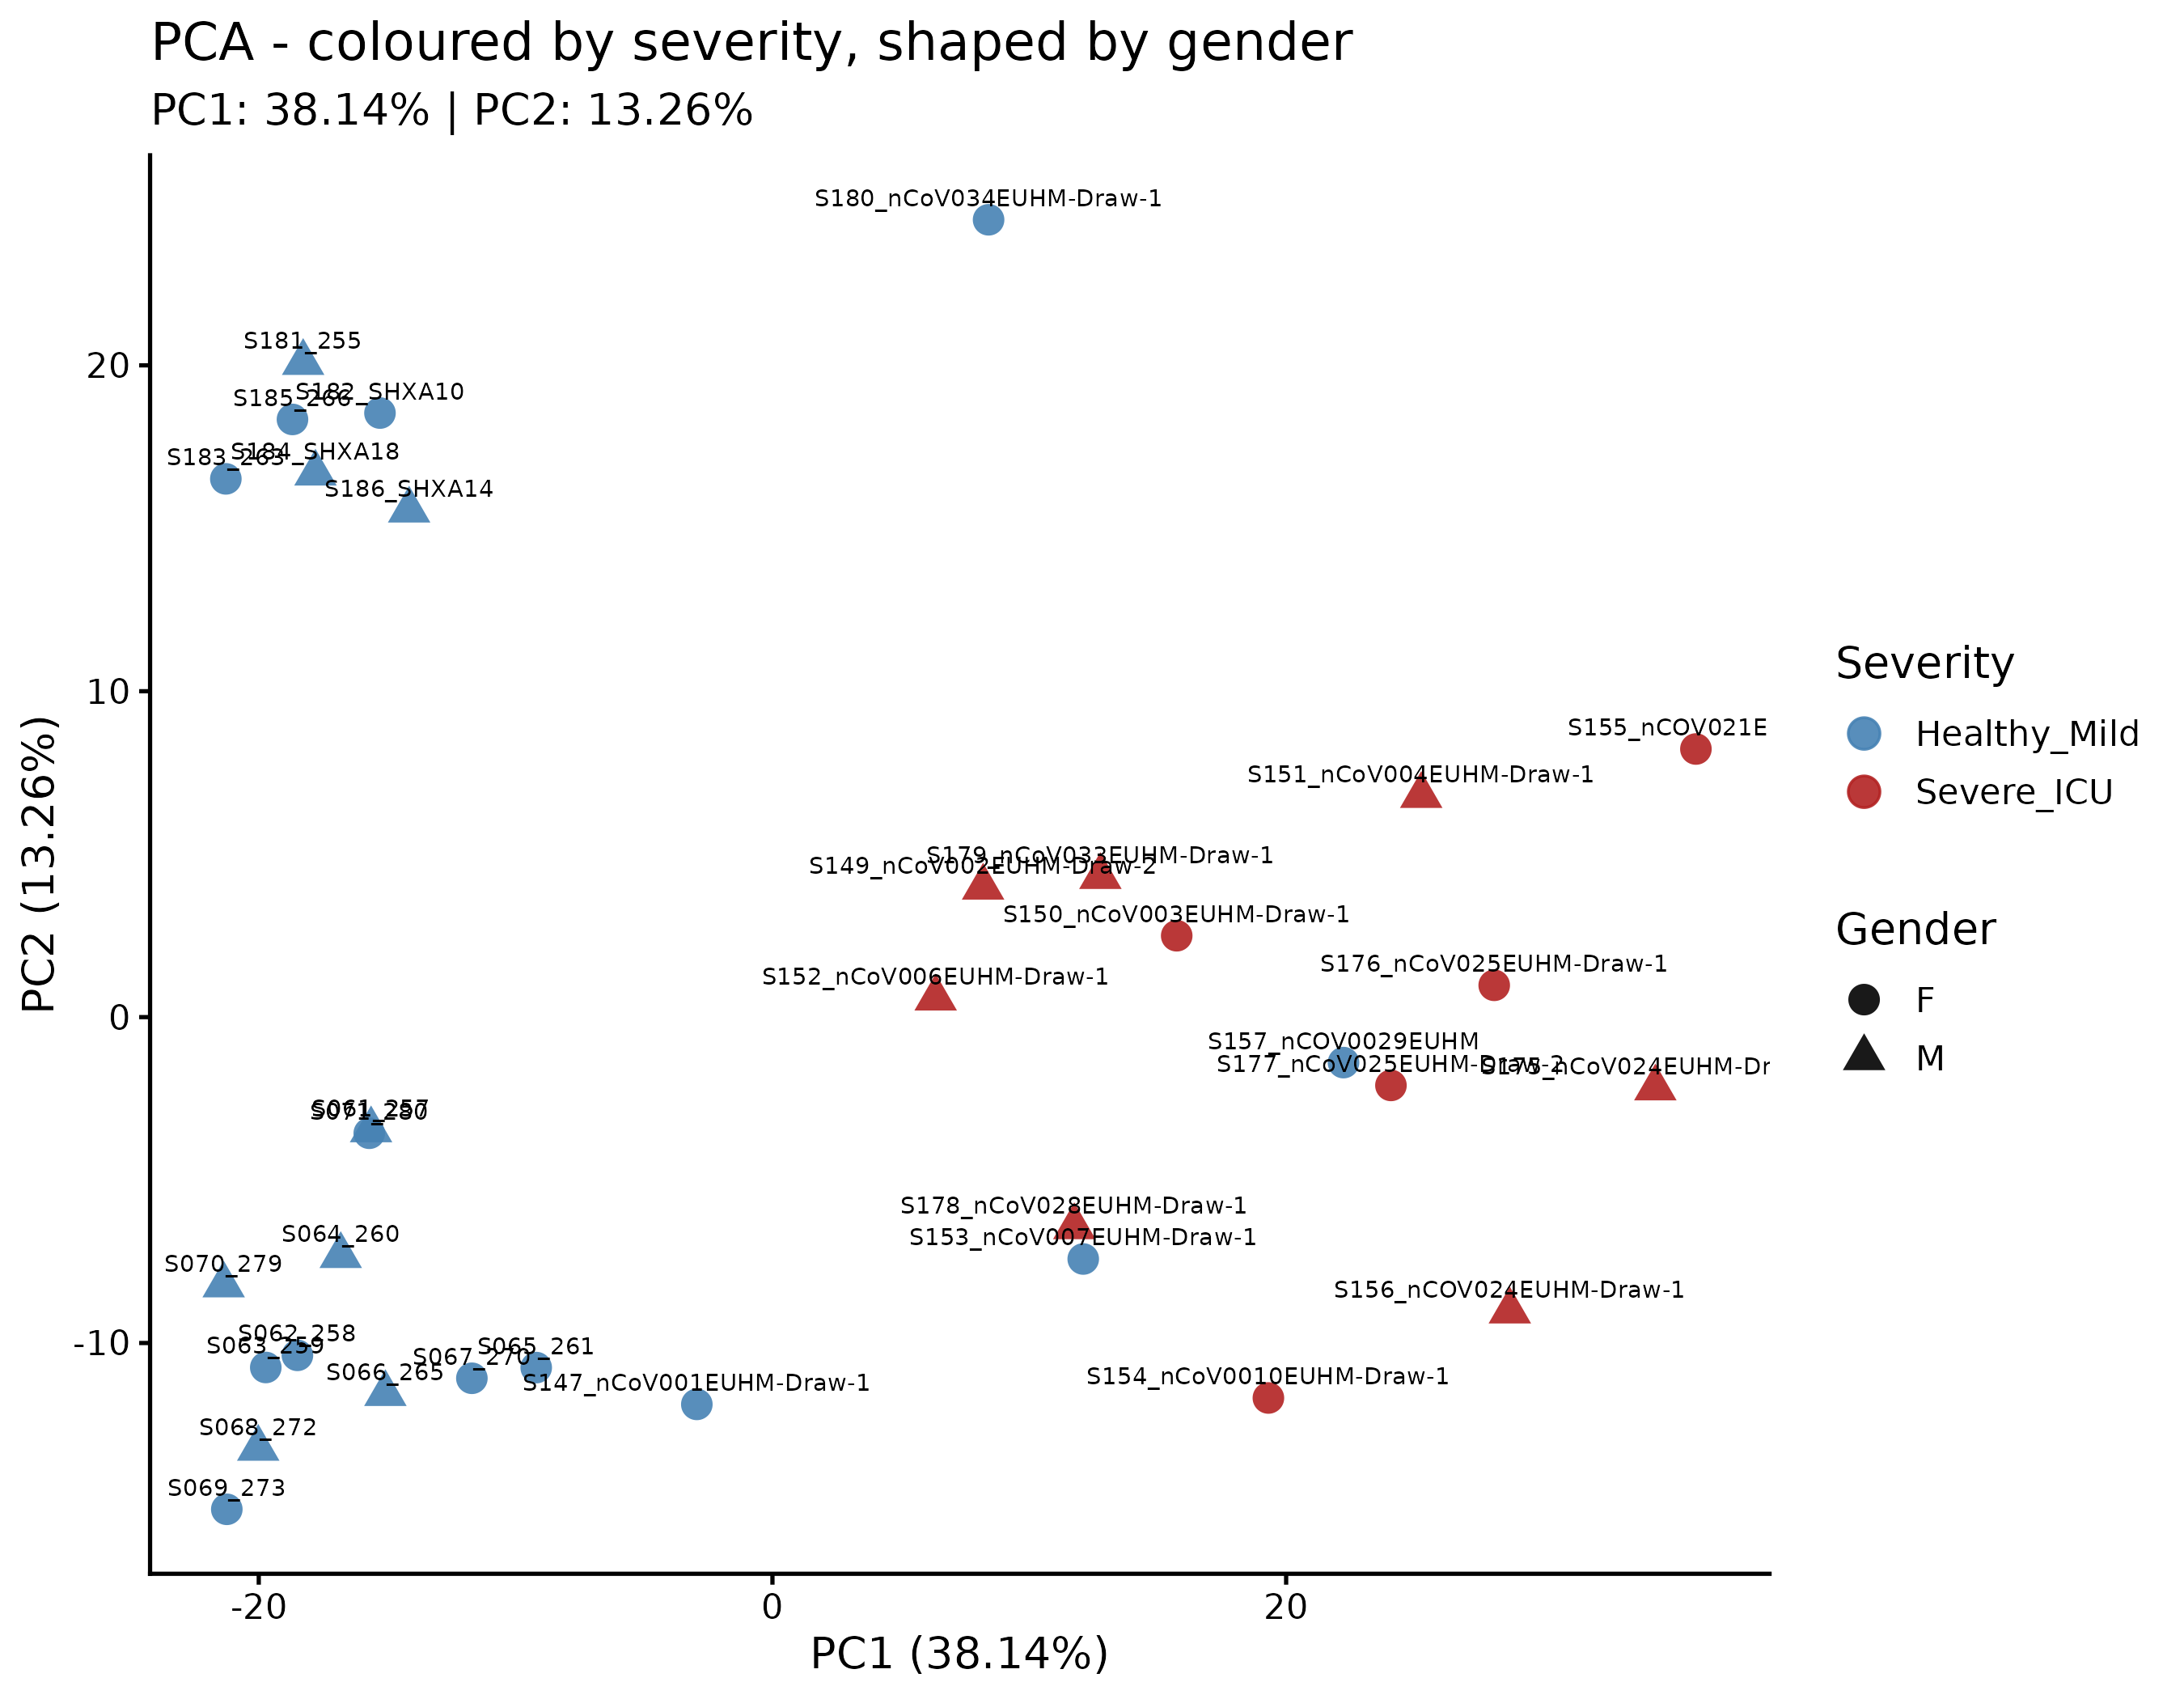
\includegraphics[width=0.9\textwidth]{plots/phase11/phase11_PCA_severity_gender.png}
\end{center}

Circles = Female; triangles = Male.

\begin{itemize}[nosep]
  \item Within the Healthy/Mild (blue) cluster, female and male samples are
        \textbf{fully intermixed}. No gender sub-cluster is visible along PC1 or PC2.
  \item The same holds within the Severe/ICU (red) cluster.
  \item \textbf{This visually confirms the Phase 9 finding} ($r = 0.97$ between the
        simple and gender-adjusted models): gender explains very little of the
        transcriptomic variance. The dominant structure is severity, not gender.
\end{itemize}

\subsubsection*{Step 5e — PC1 vs PC3}

\begin{center}
  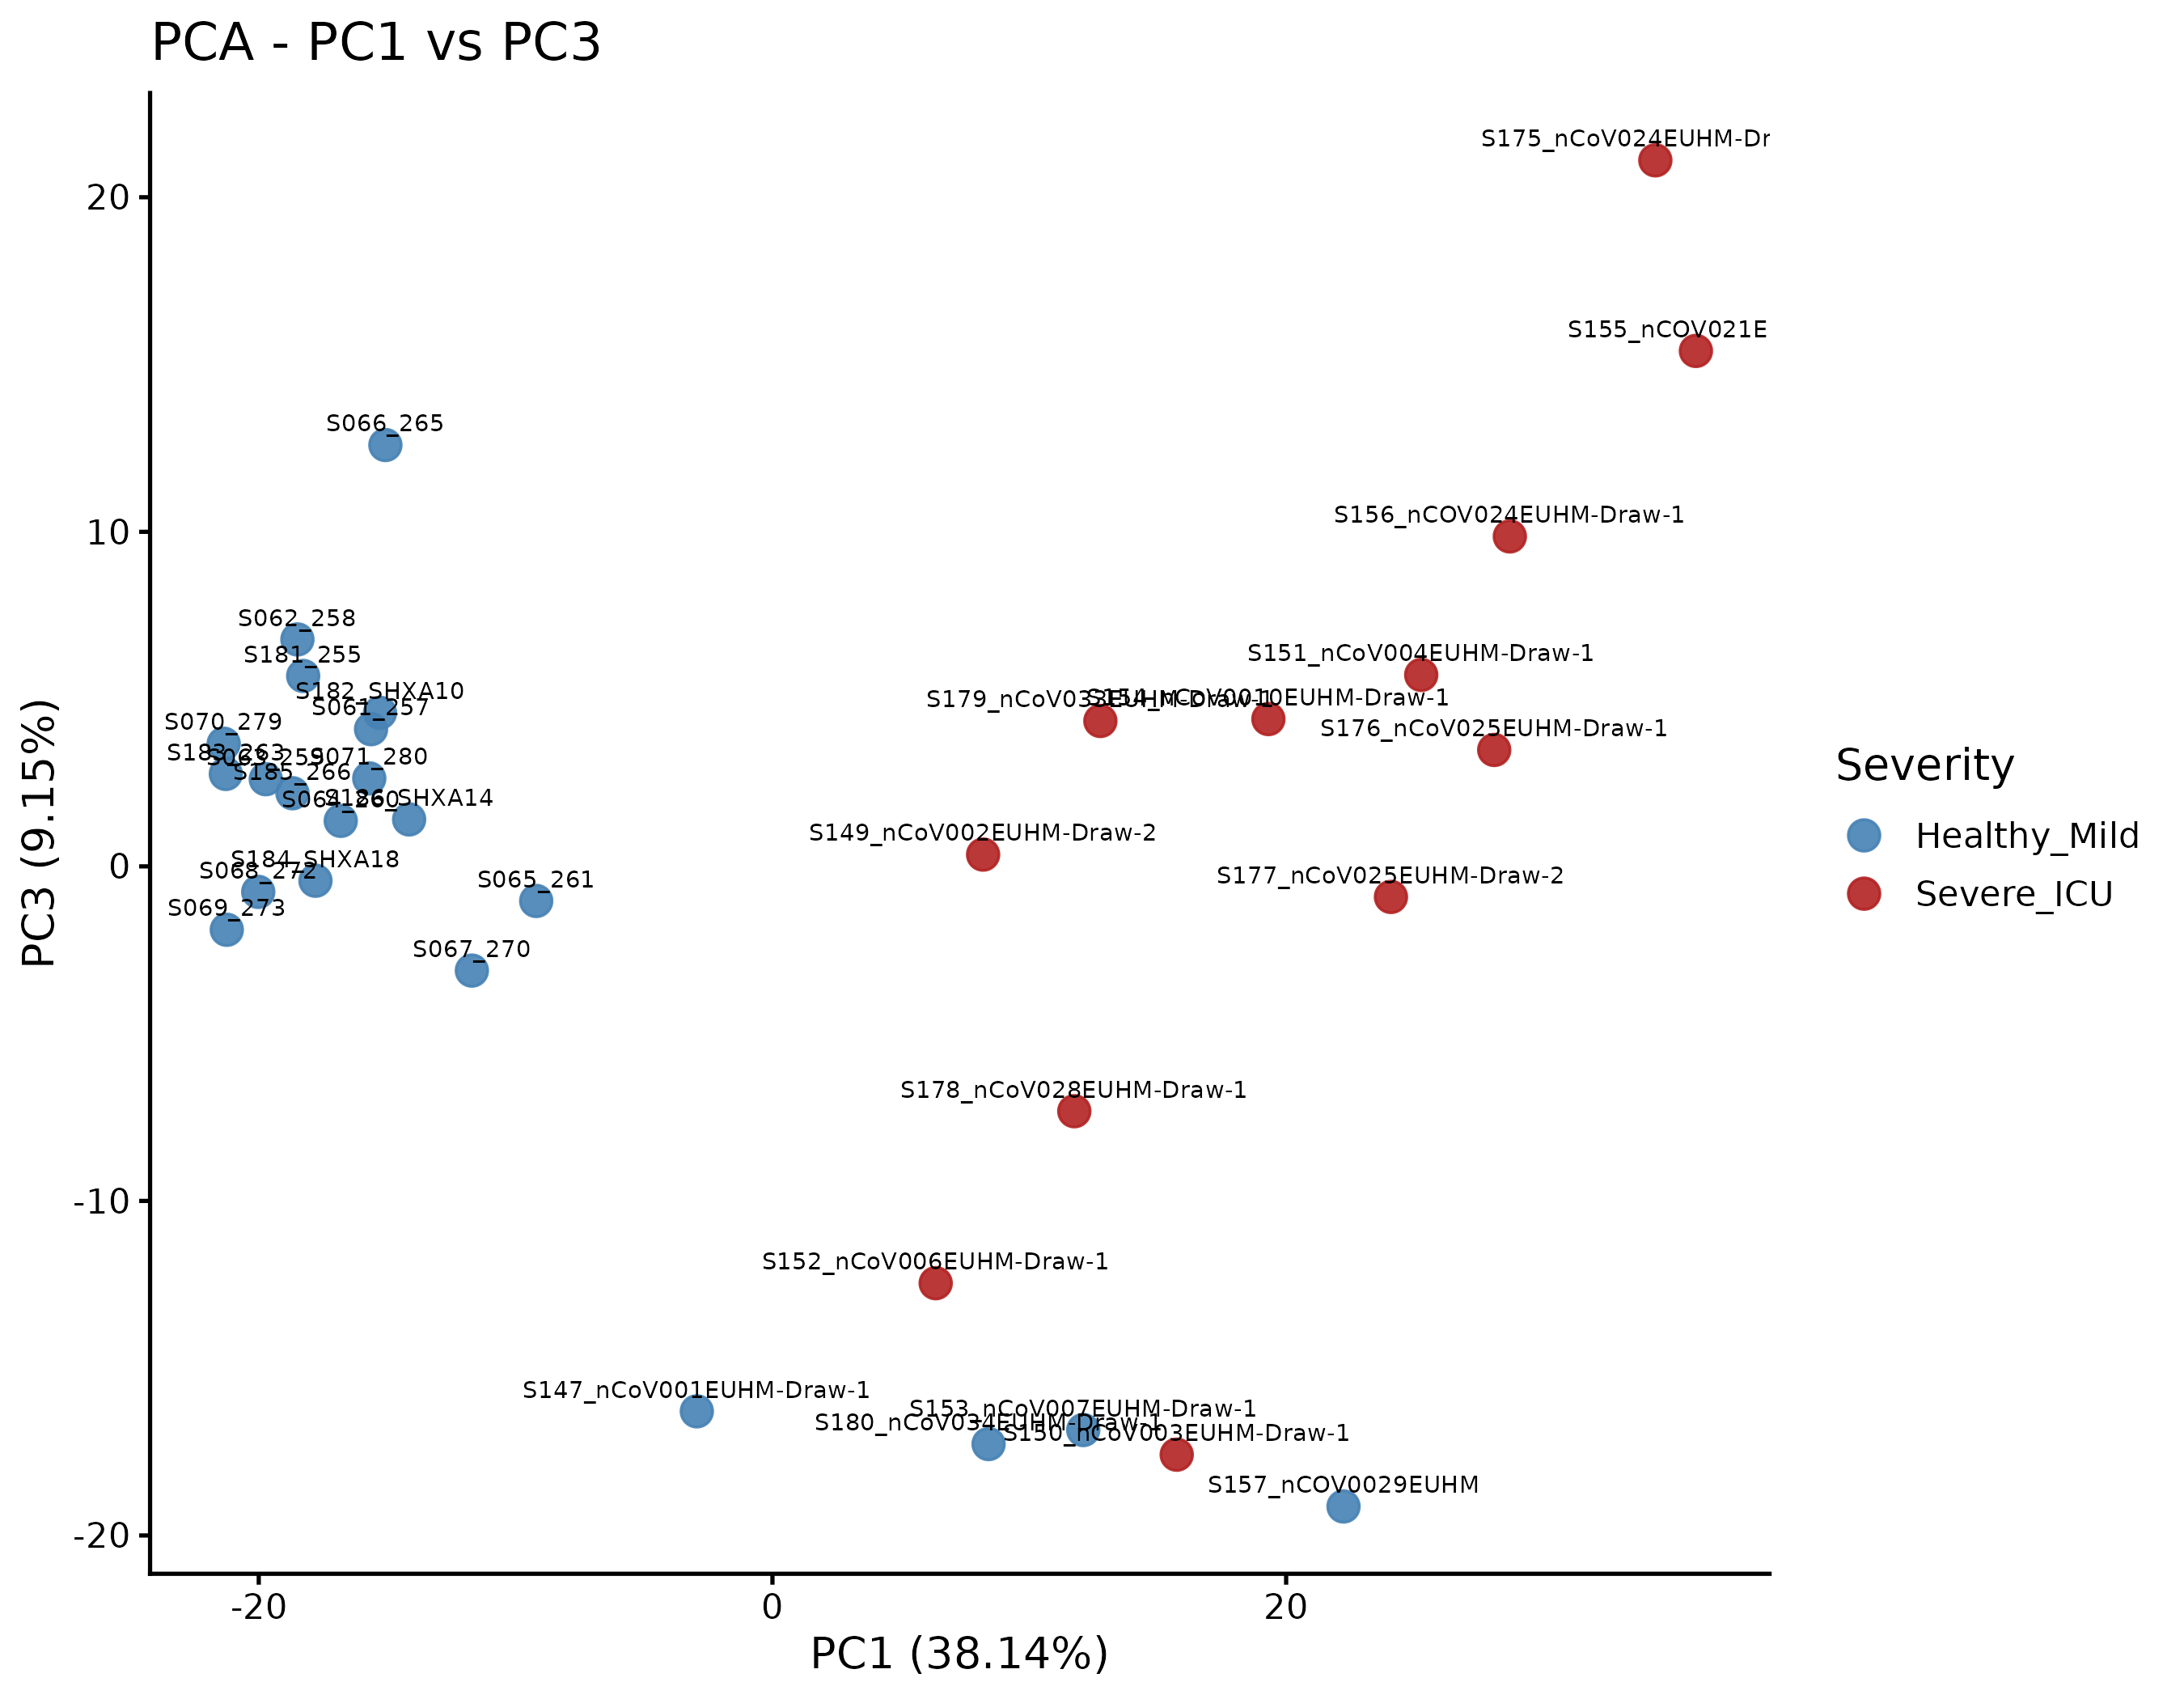
\includegraphics[width=0.9\textwidth]{plots/phase11/phase11_PCA_PC1_PC3.png}
\end{center}

\begin{itemize}[nosep]
  \item PC1 (x-axis) still separates the groups cleanly.
  \item PC3 (y-axis, 9.15\%) shows \textbf{no severity structure} — both groups
        scatter broadly in both directions with no trend.
  \item Two Severe samples (S175\_nCoV024, S155\_nCOV021E) and one Healthy sample
        (S066\_265) reach extreme PC3 values ($\pm12$--$20$). These are individual
        donor outliers on the third axis, not a coherent group effect.
  \item \textbf{Conclusion:} severity is captured entirely by PC1. All higher PCs
        represent within-condition biological variability and individual donor
        differences.
\end{itemize}

\subsection{Sample similarity — correlation and distance matrices
  \small\normalfont\textit{(Steps 6--7)}}

If PCA is too abstract, the correlation and distance matrices provide a direct,
concrete view: how similar is every sample to every other sample?

\subsubsection*{Step 6 — Sample-to-sample Pearson correlation matrix}

\begin{center}
  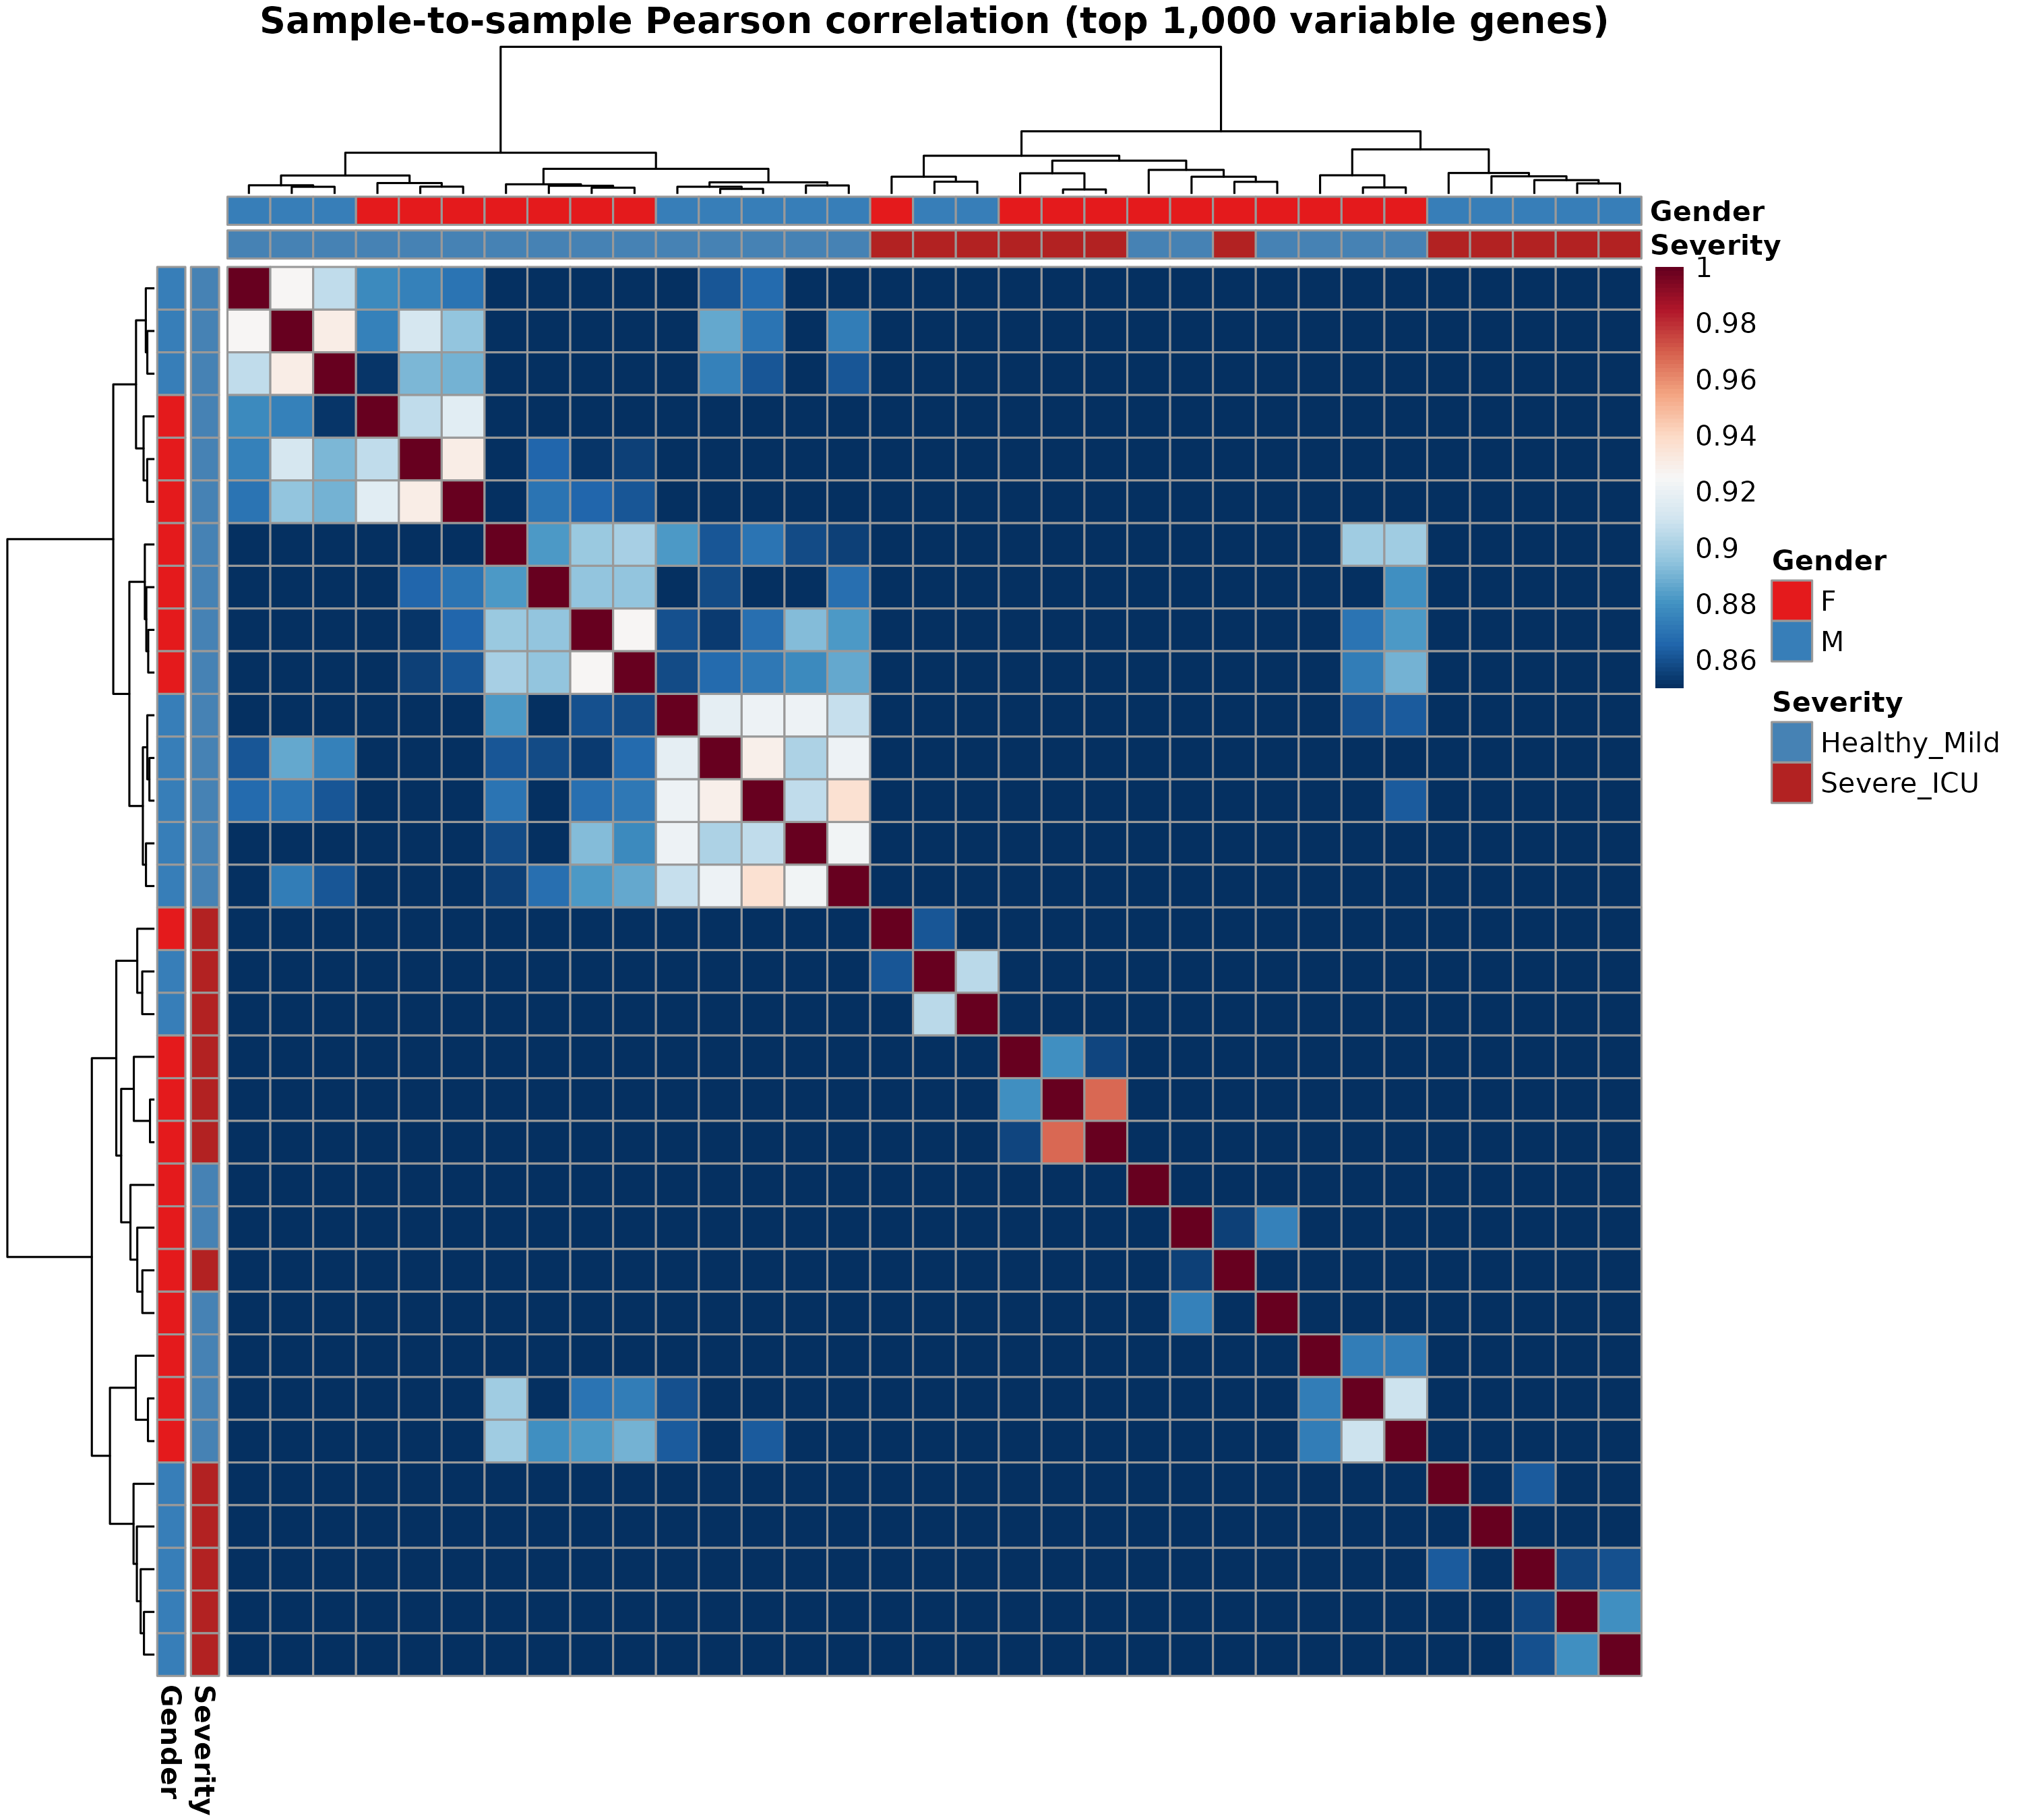
\includegraphics[width=\textwidth]{plots/phase11/phase11_correlation_matrix.png}
\end{center}

Each cell shows the Pearson correlation between two samples:
warm/white = highly similar ($r \approx 0.98$--$1.0$); dark blue = dissimilar
($r \approx 0.86$--$0.90$). Rows and columns are ordered by hierarchical clustering.

\begin{itemize}[nosep]
  \item \textbf{Two clear blocks on the diagonal:} a Severe block (top-left) and a
        Healthy block (bottom-right). Within each block samples are warm; between
        blocks they are uniformly cold.
  \item \textbf{Within the Severe block:} a sub-cluster of $\sim$5--6 samples shows
        near-white correlation ($r \approx 0.99$) — very tightly similar donors.
        The remaining Severe samples are slightly more spread.
  \item \textbf{Every cross-block pair} (top-right and bottom-left corners) is dark
        blue — every Severe sample is substantially different from every Healthy sample.
        There is no Severe sample that ``looks like'' any Healthy sample in pairwise
        correlation.
  \item \textbf{Gender annotation} at the top shows females and males intermixed
        within each block — no gender-driven sub-structure.
\end{itemize}

\textbf{Reading the result:} 1,000 genes are enough to distinguish any Severe
sample from any Healthy sample by correlation alone, without any label information.

\subsubsection*{Step 7 — Sample-to-sample Euclidean distance matrix}

\begin{center}
  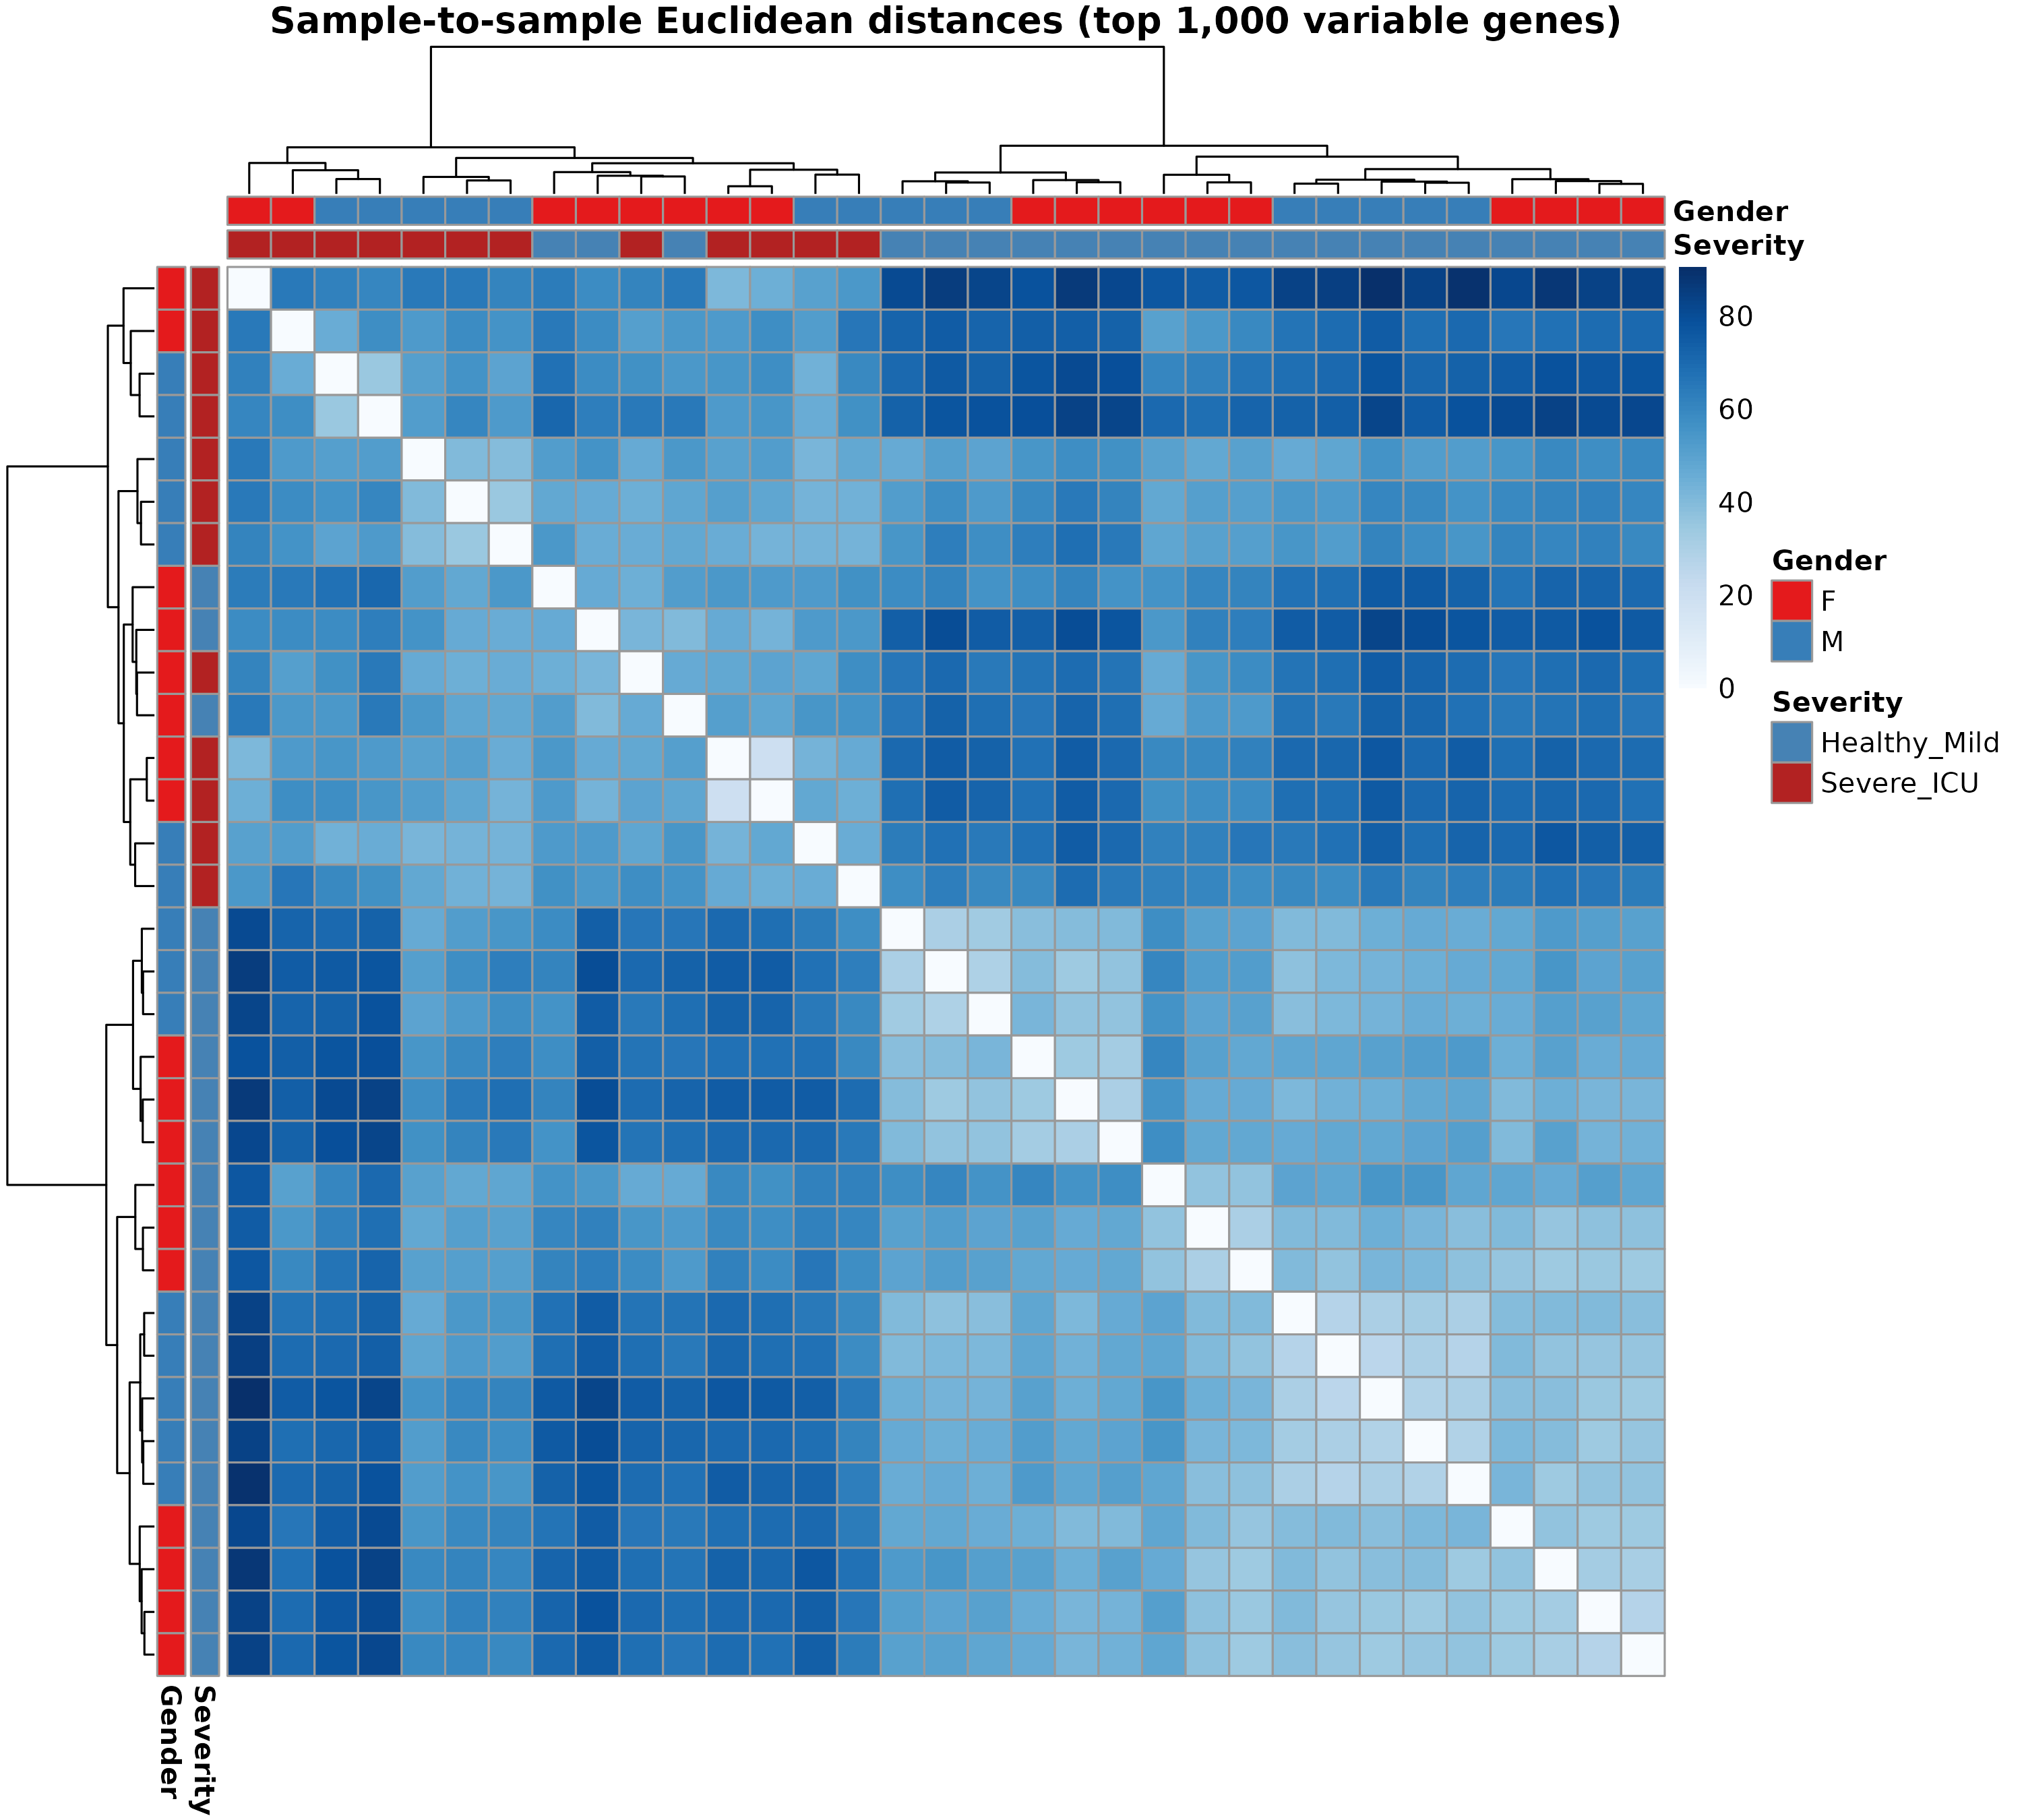
\includegraphics[width=\textwidth]{plots/phase11/phase11_distance_matrix.png}
\end{center}

Distance is the complement of correlation: high distance = dissimilar = dark blue;
zero = diagonal (self) = white.

\begin{itemize}[nosep]
  \item The same two-block structure appears, now as \textbf{two light (small distance)
        diagonal blocks} separated by \textbf{dark (large distance) off-diagonal corners}.
  \item Within-Severe distances: 20--40 (light blue). Within-Healthy: 20--30
        (very light). Between-group distances: 60--90 (dark blue).
  \item The Healthy group forms the tighter block — healthy blood transcriptomes
        are in a more similar baseline state. The Severe group is slightly more
        heterogeneous, again consistent with disease variability between patients.
\end{itemize}

\subsection{Clustering \small\normalfont\textit{(Steps 8--9)}}

\subsubsection*{Step 8 — Hierarchical clustering (Ward.D2)}

\begin{center}
  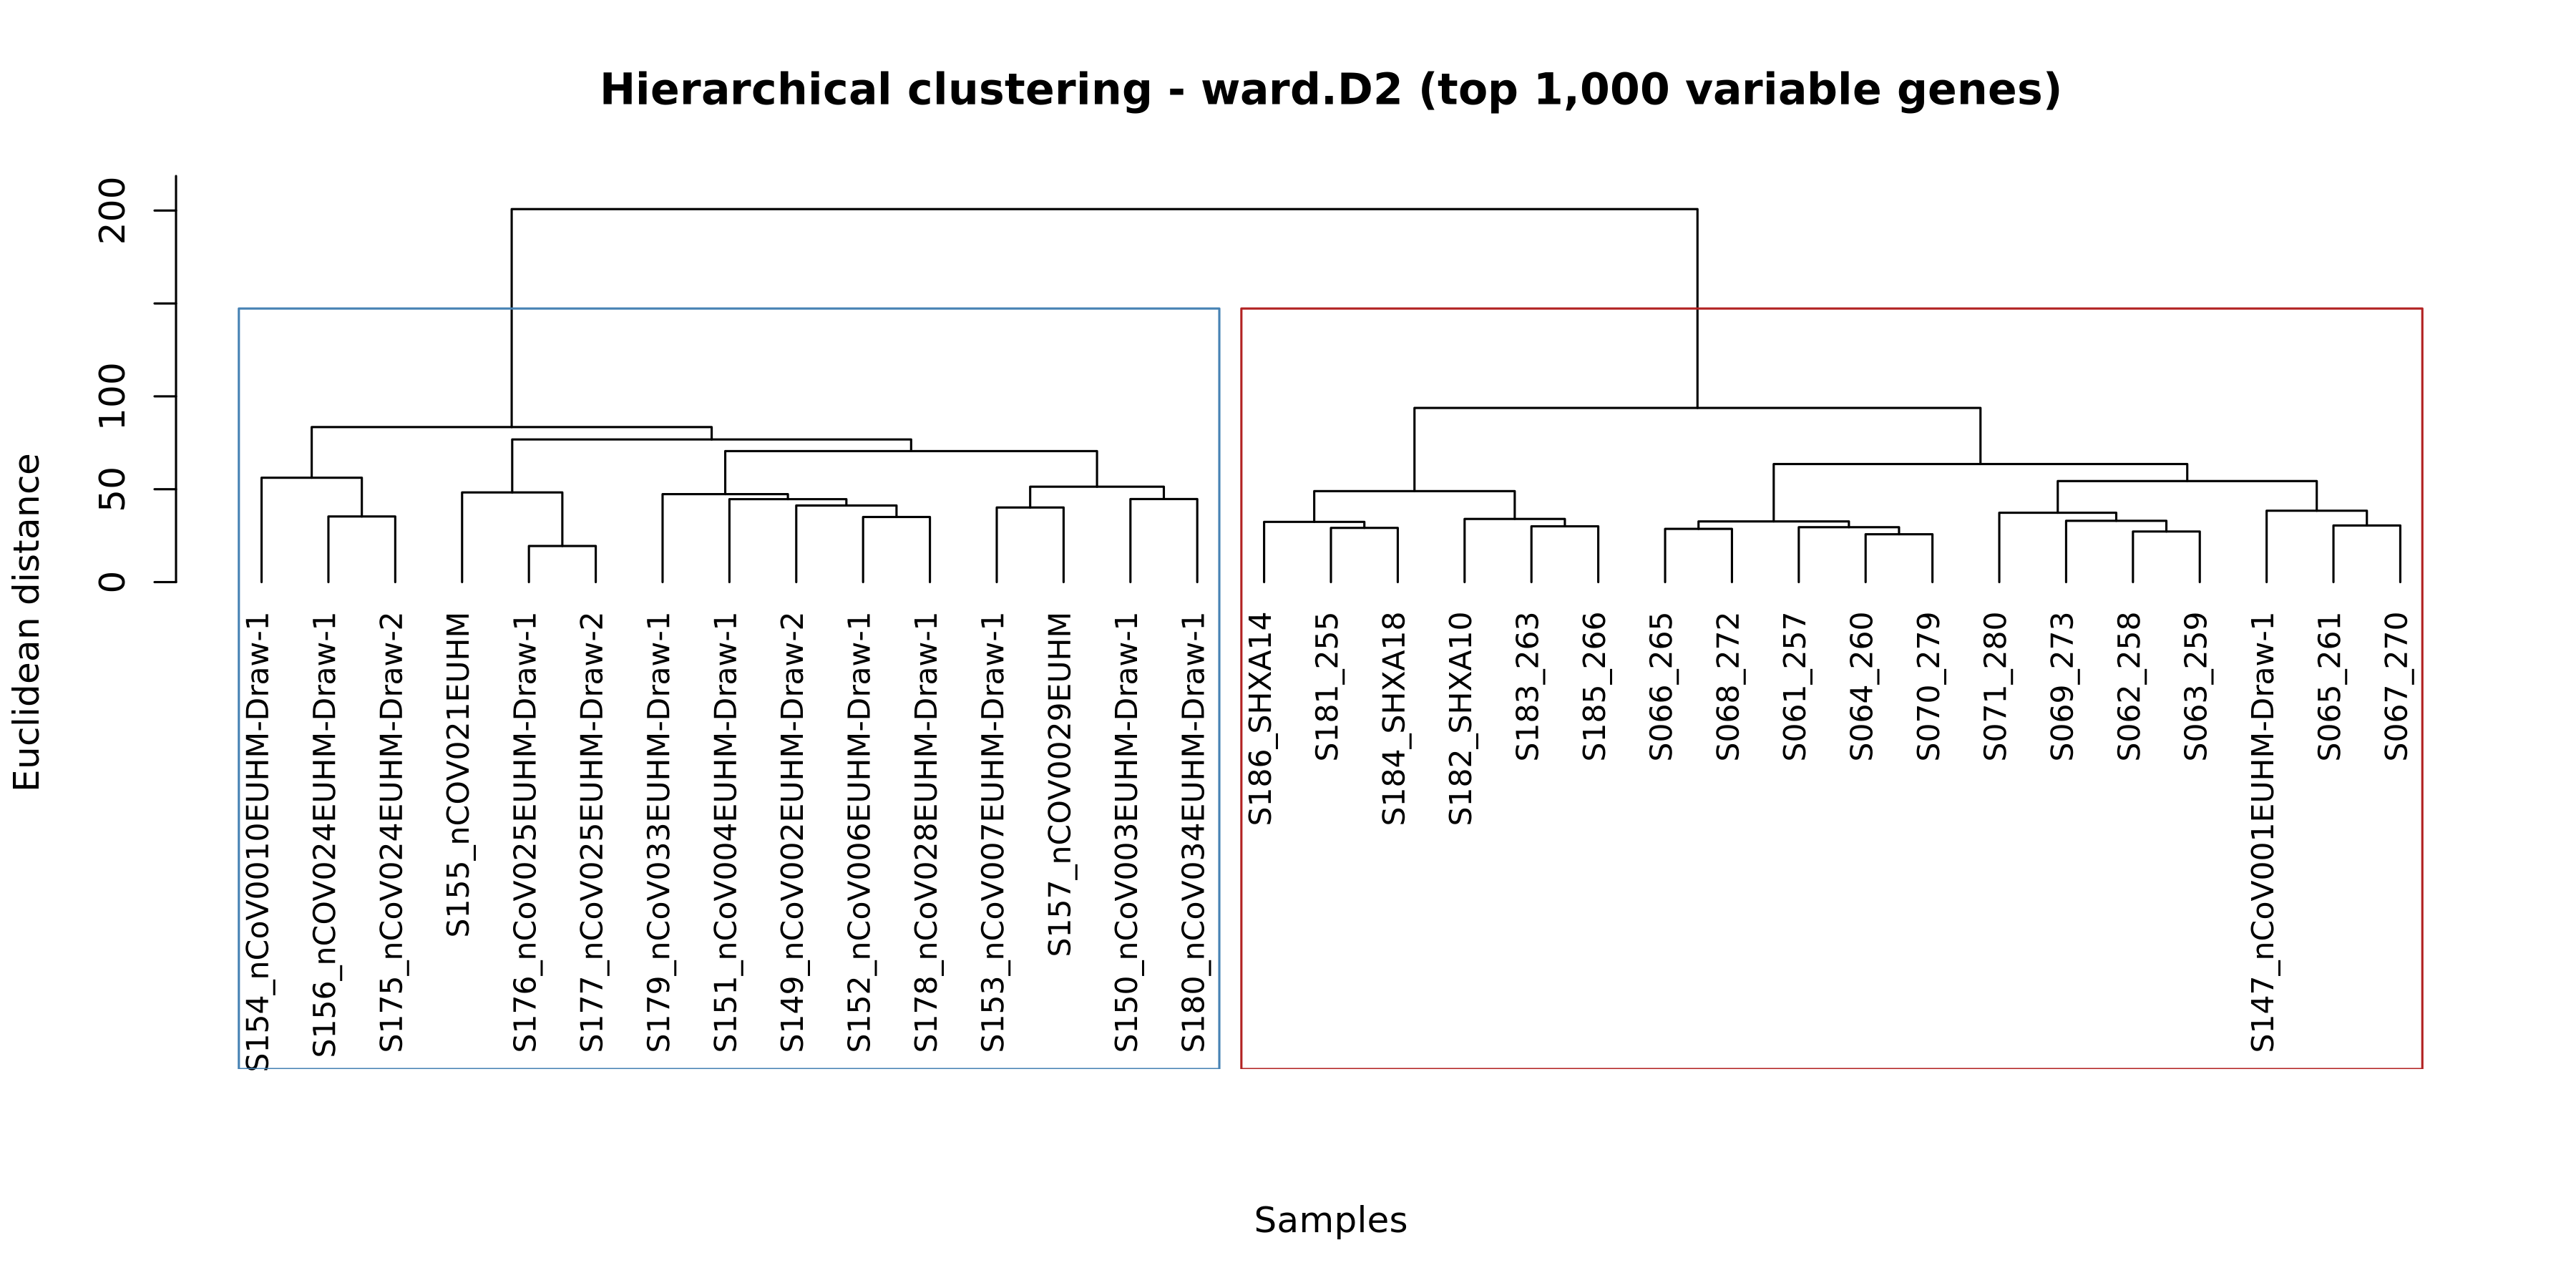
\includegraphics[width=\textwidth]{plots/phase11/phase11_hierarchical_clustering.png}
\end{center}

The dendrogram connects samples by similarity, bottom-up. Samples merging at low
height are very similar; those merging near the top are only grouped because there
is no better alternative. The two coloured boxes mark the $k = 2$ cut.

\begin{itemize}[nosep]
  \item \textbf{Left branch (blue box):} contains almost exclusively Severe/ICU
        samples (all nCoV-prefixed labels). Their sub-branches merge at heights of
        30--80; the two main sub-branches join at $\approx$175. This is the Severe cluster.
  \item \textbf{Right branch (red box):} contains almost exclusively Healthy/Mild
        samples (SHXA- and numbered labels). Their internal branches merge at heights
        of 10--30 — tighter than Severe, consistent with the lower within-group
        distances seen in the distance matrix.
  \item \textbf{One misclassification:} S147\_nCoV001EUHM-Draw-1 (a Severe sample)
        is placed in the Healthy branch. Looking at the PC1 vs PC2 plot, this sample
        sits on the negative-PC1 (Healthy) side — its transcriptome is genuinely
        closer to Healthy samples than to typical Severe samples.
        This is a biologically interesting outlier: one Severe patient whose blood
        profile does not match the typical severe signature. Early-stage disease,
        sample timing, or patient-specific variation are plausible explanations.
  \item \textbf{Accuracy: 32/33 samples correctly grouped (97\%)} based on gene
        expression alone with no label input.
\end{itemize}

\subsubsection*{K-means elbow plot}

\begin{center}
  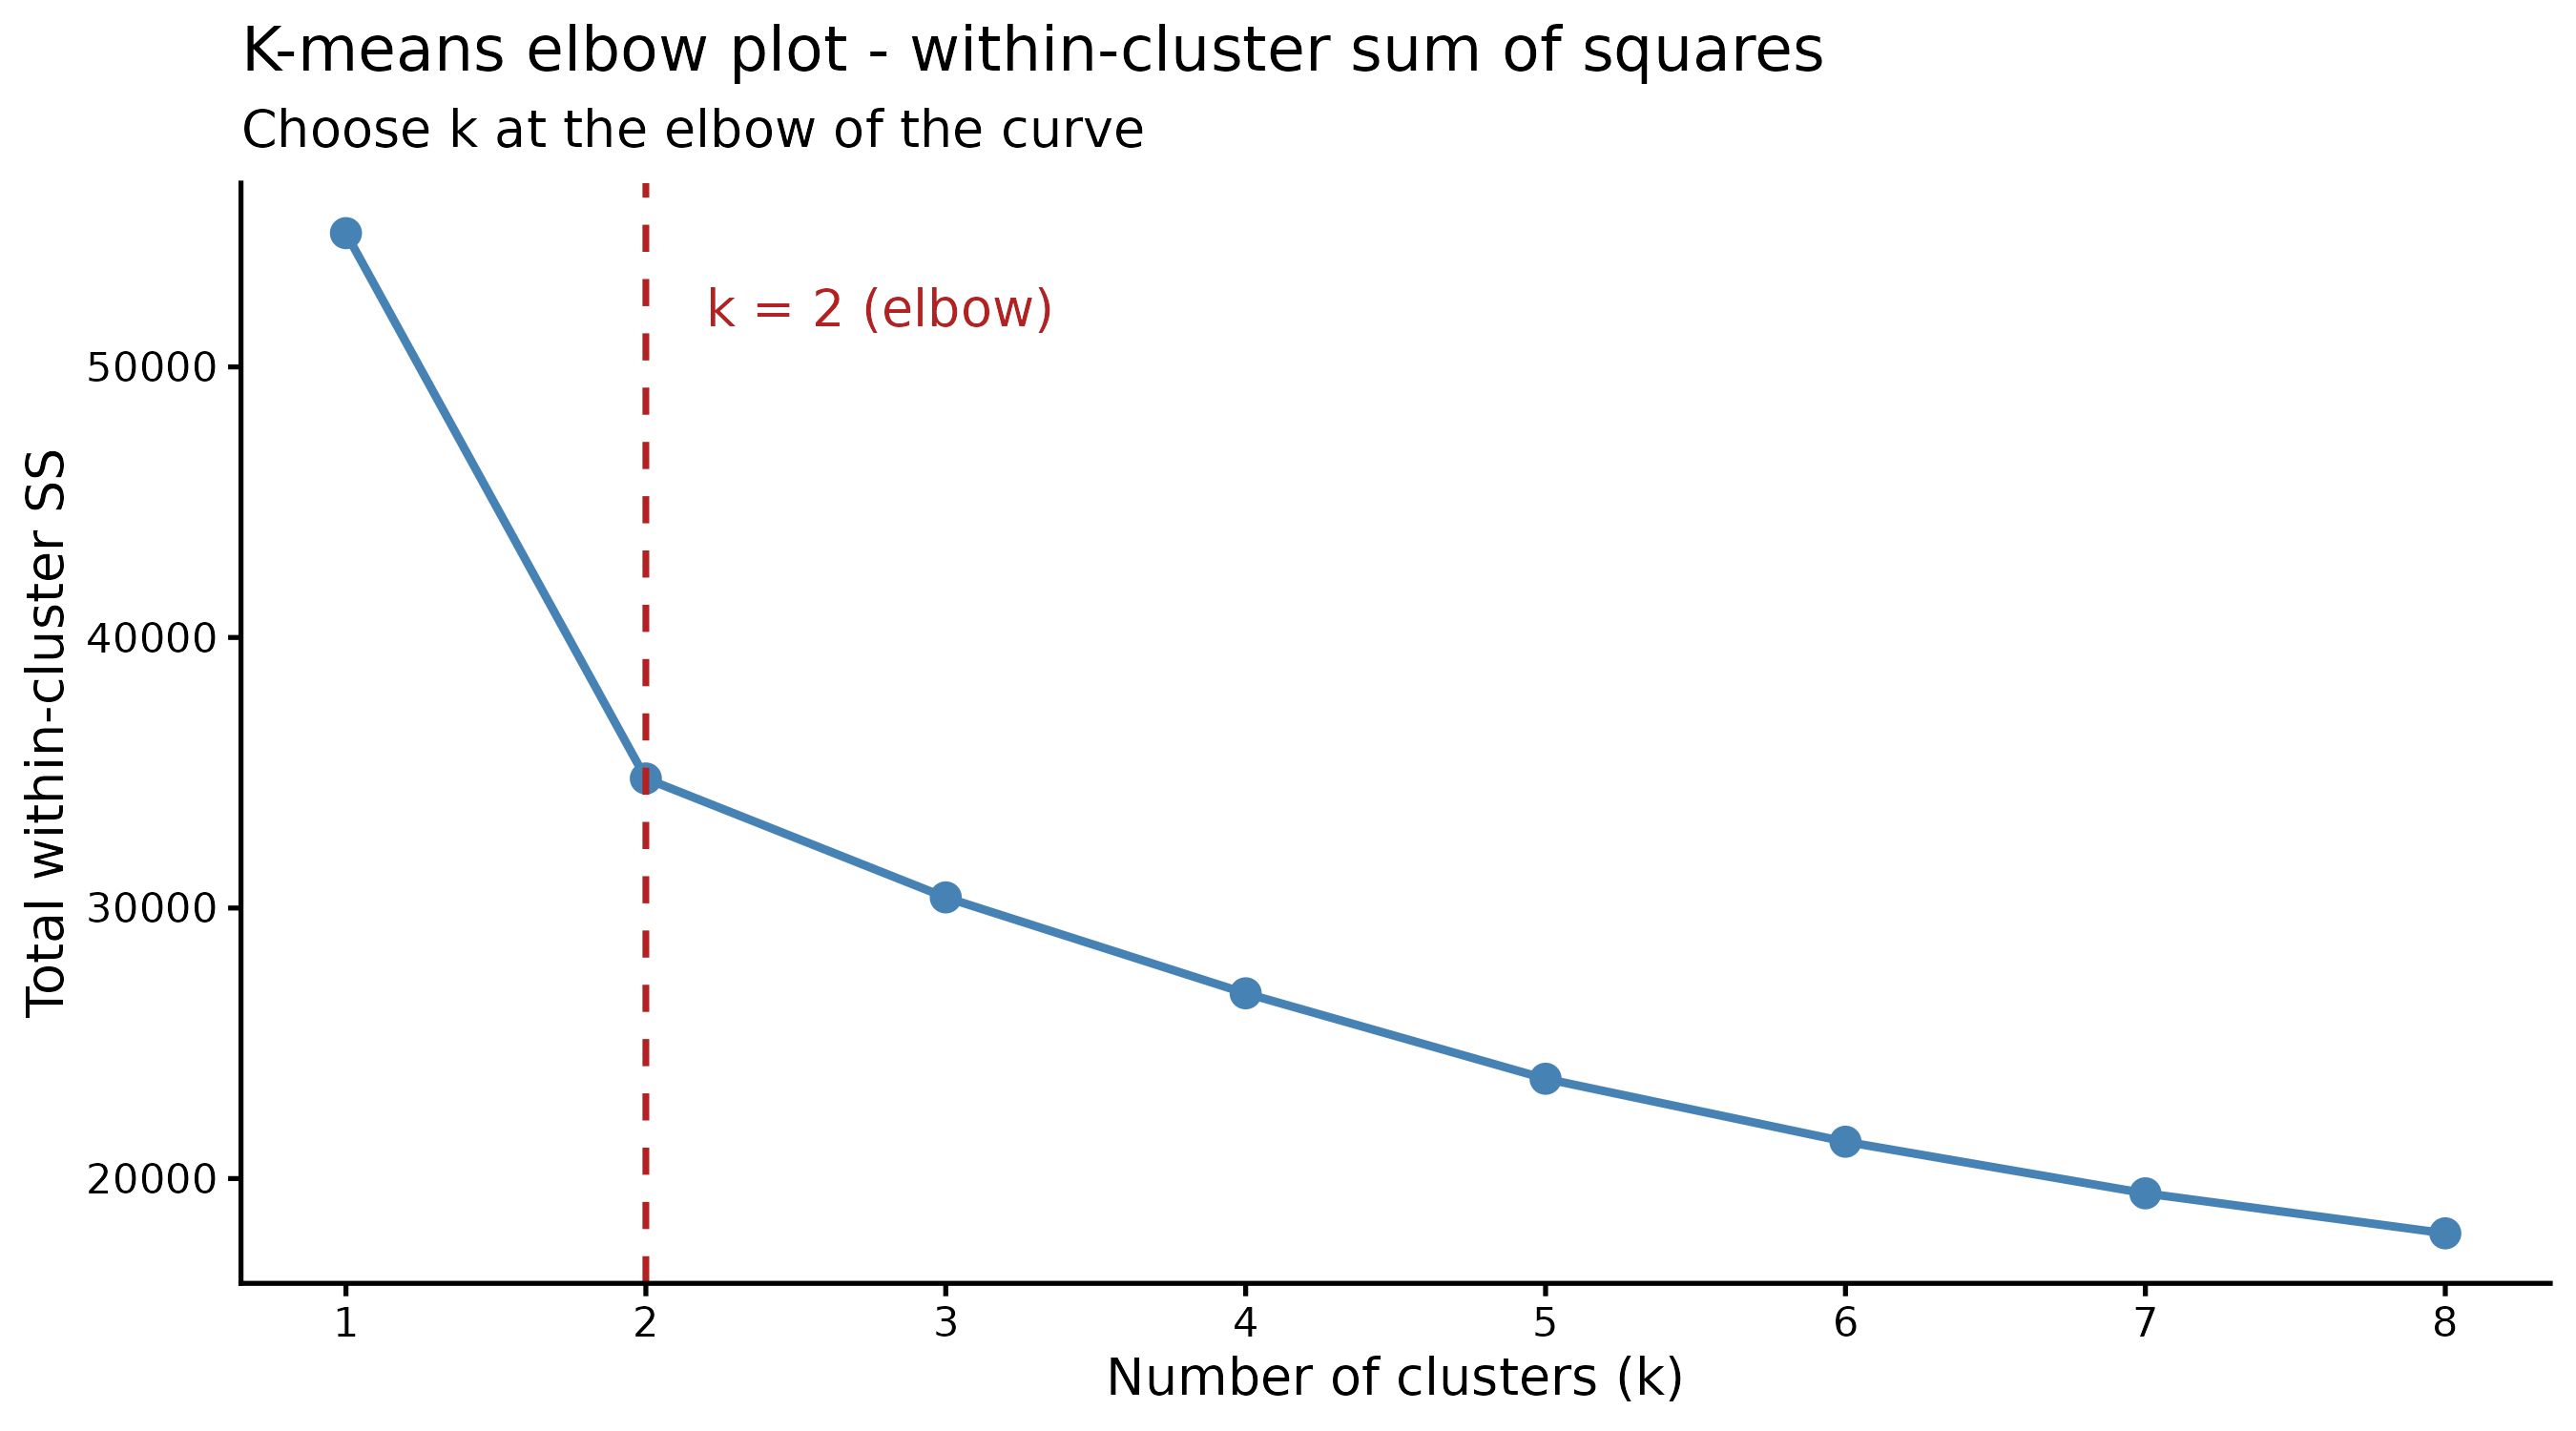
\includegraphics[width=0.85\textwidth]{plots/phase11/phase11_kmeans_elbow.png}
\end{center}

K-means partitions samples into $k$ groups by minimizing within-group spread.
The elbow plot shows how much the total within-cluster variance drops as $k$ increases.

\begin{itemize}[nosep]
  \item $k = 1 \to k = 2$: within-cluster SS drops from $\approx$55,000 to
        $\approx$35,000 — a \textbf{large, sharp drop}.
  \item $k = 3, 4, \ldots$: slow, nearly linear decrease with no clear bend.
  \item \textbf{The elbow is unambiguously at $k = 2$}, confirming that two is
        the natural number of groups in this dataset — consistent with the two
        severity conditions.
\end{itemize}

\subsubsection*{K-means $k = 2$ visualization}

\begin{center}
  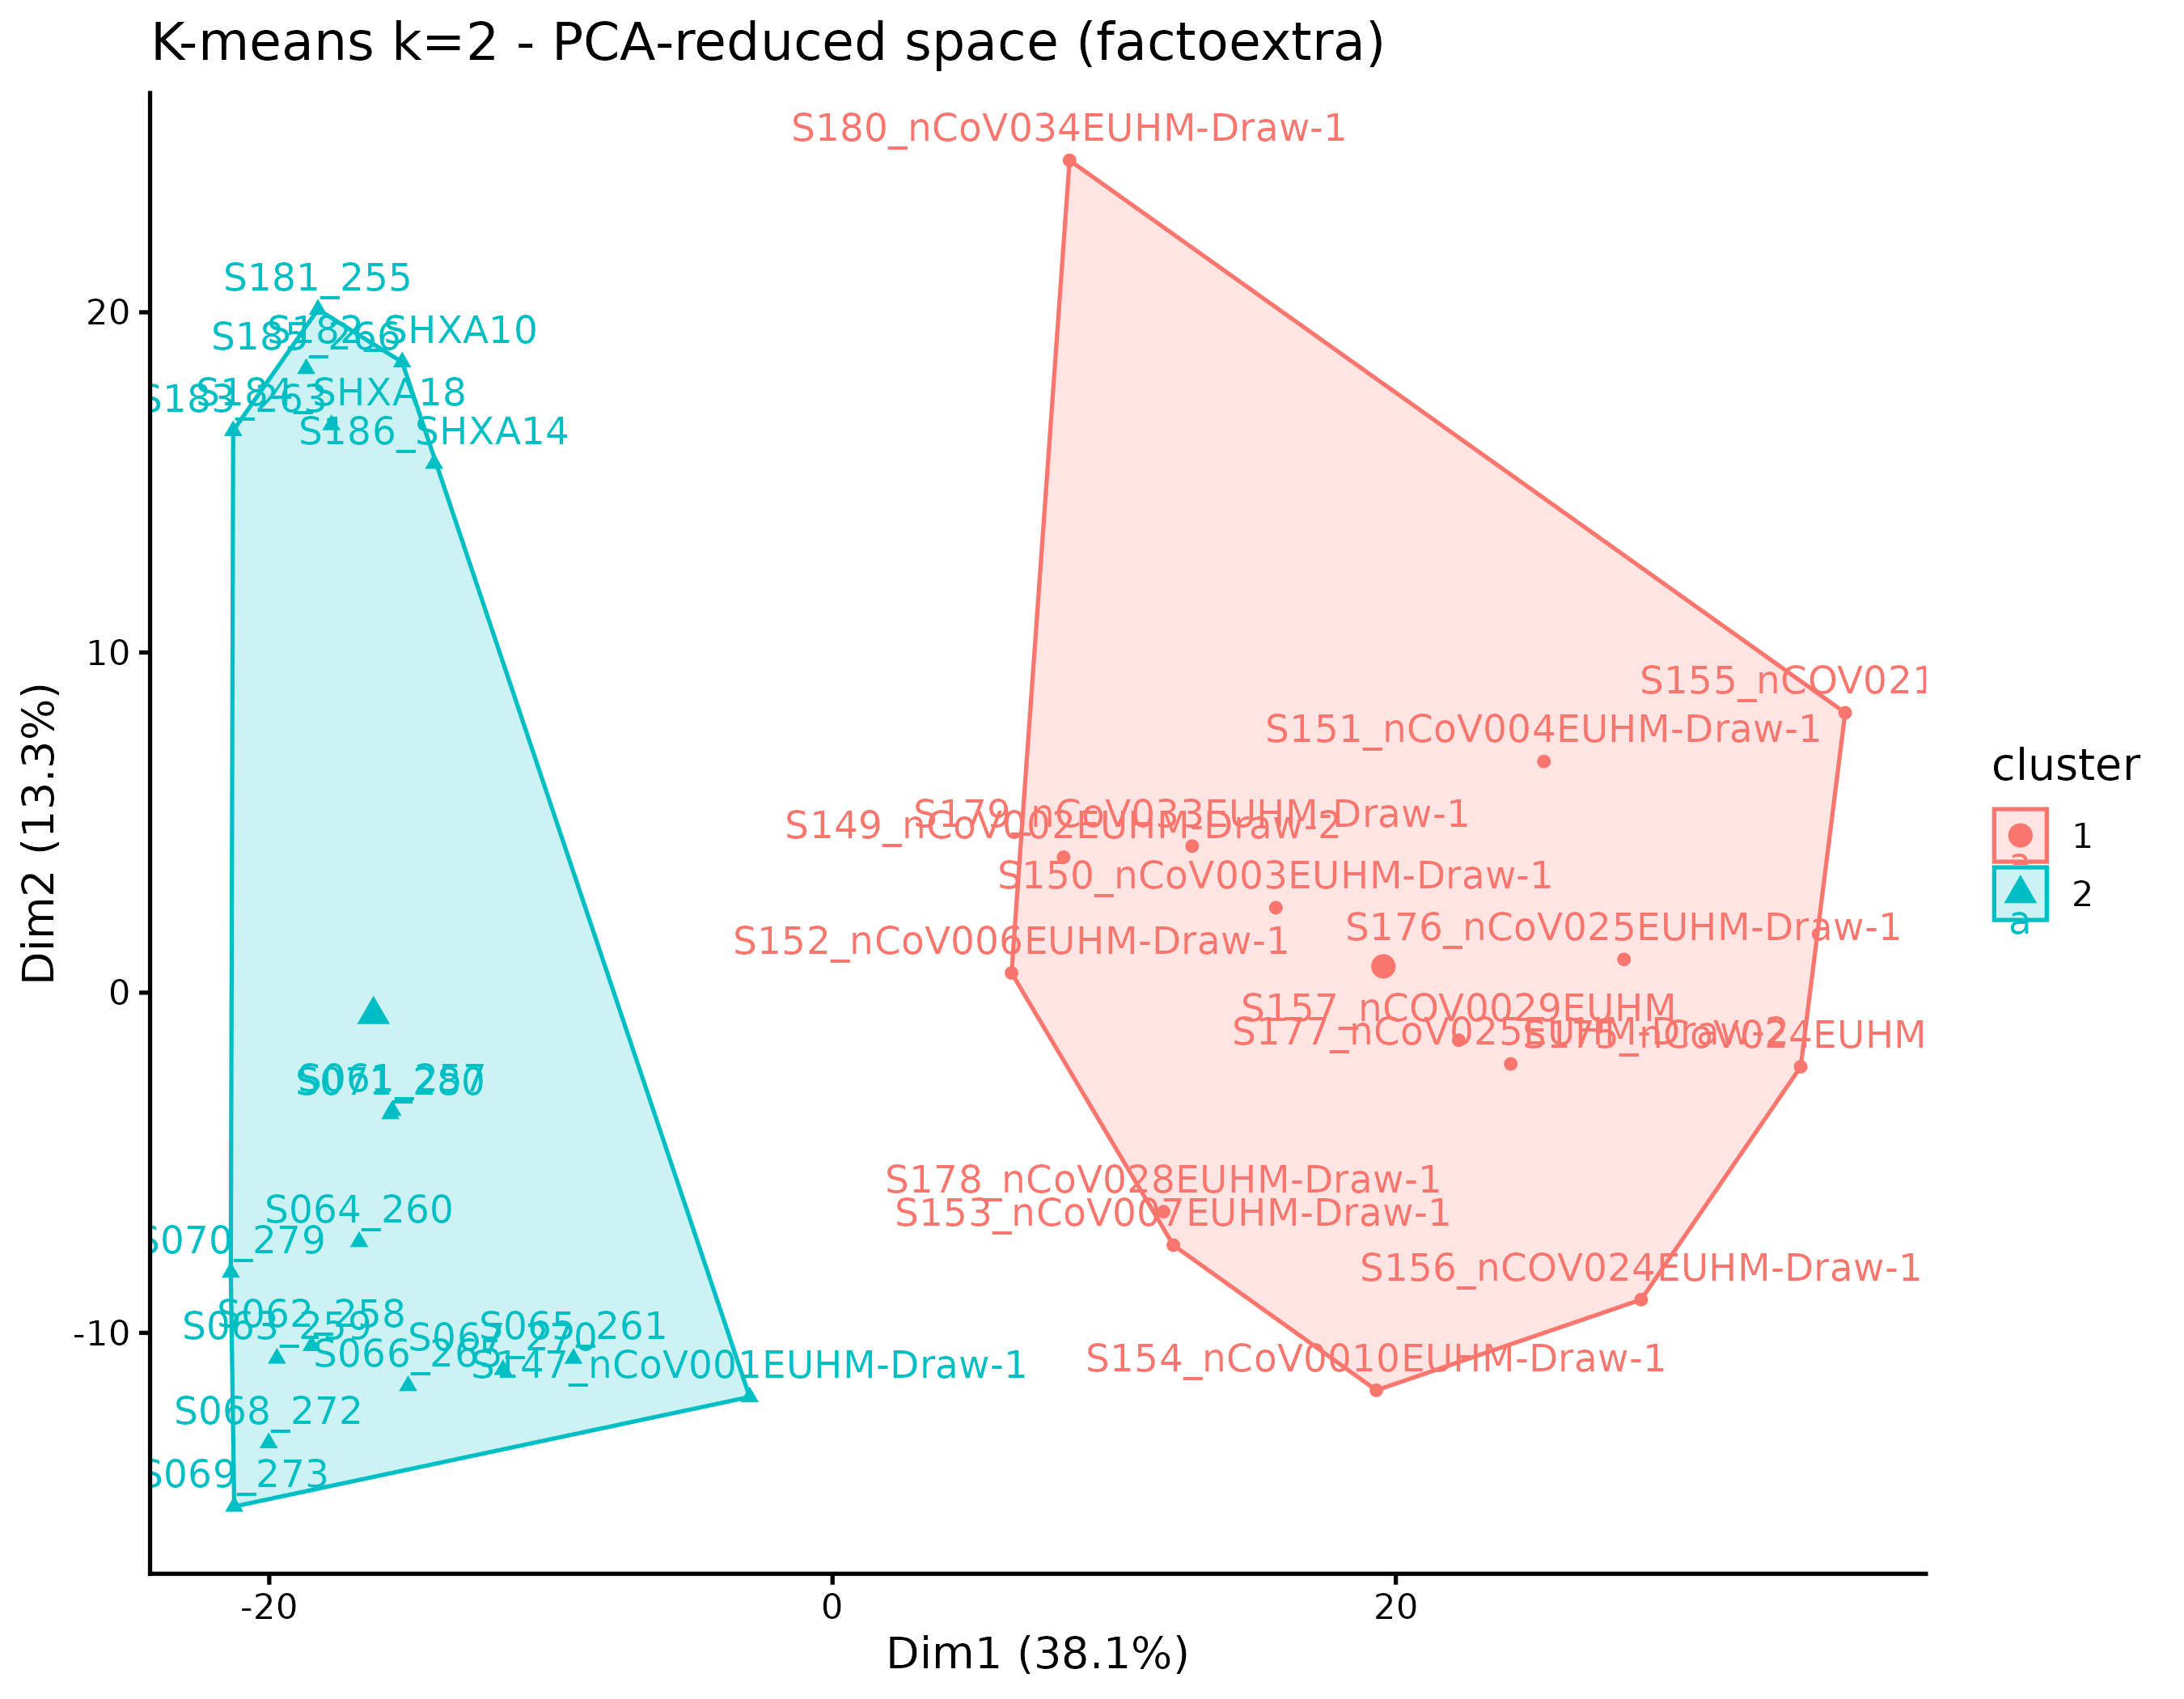
\includegraphics[width=0.9\textwidth]{plots/phase11/phase11_kmeans_fviz.png}
\end{center}

The two k-means clusters plotted in PCA space, with convex hulls showing each
cluster's spread.

\begin{itemize}[nosep]
  \item \textbf{The two hulls do not overlap.} Cluster 1 (red/salmon, right) occupies
        positive PC1; cluster 2 (teal, left) occupies negative PC1.
  \item All Healthy/Mild samples fall inside the teal hull; all Severe/ICU samples
        fall inside the red hull — with the same single exception (S147\_nCoV001EUHM-Draw-1
        is enclosed in the teal hull).
  \item S180\_nCoV034EUHM-Draw-1 (the PC2 outlier) is correctly enclosed in the red
        Severe hull despite its unusual vertical position.
\end{itemize}

\subsubsection*{K-means cluster vs known severity overlay}

\begin{center}
  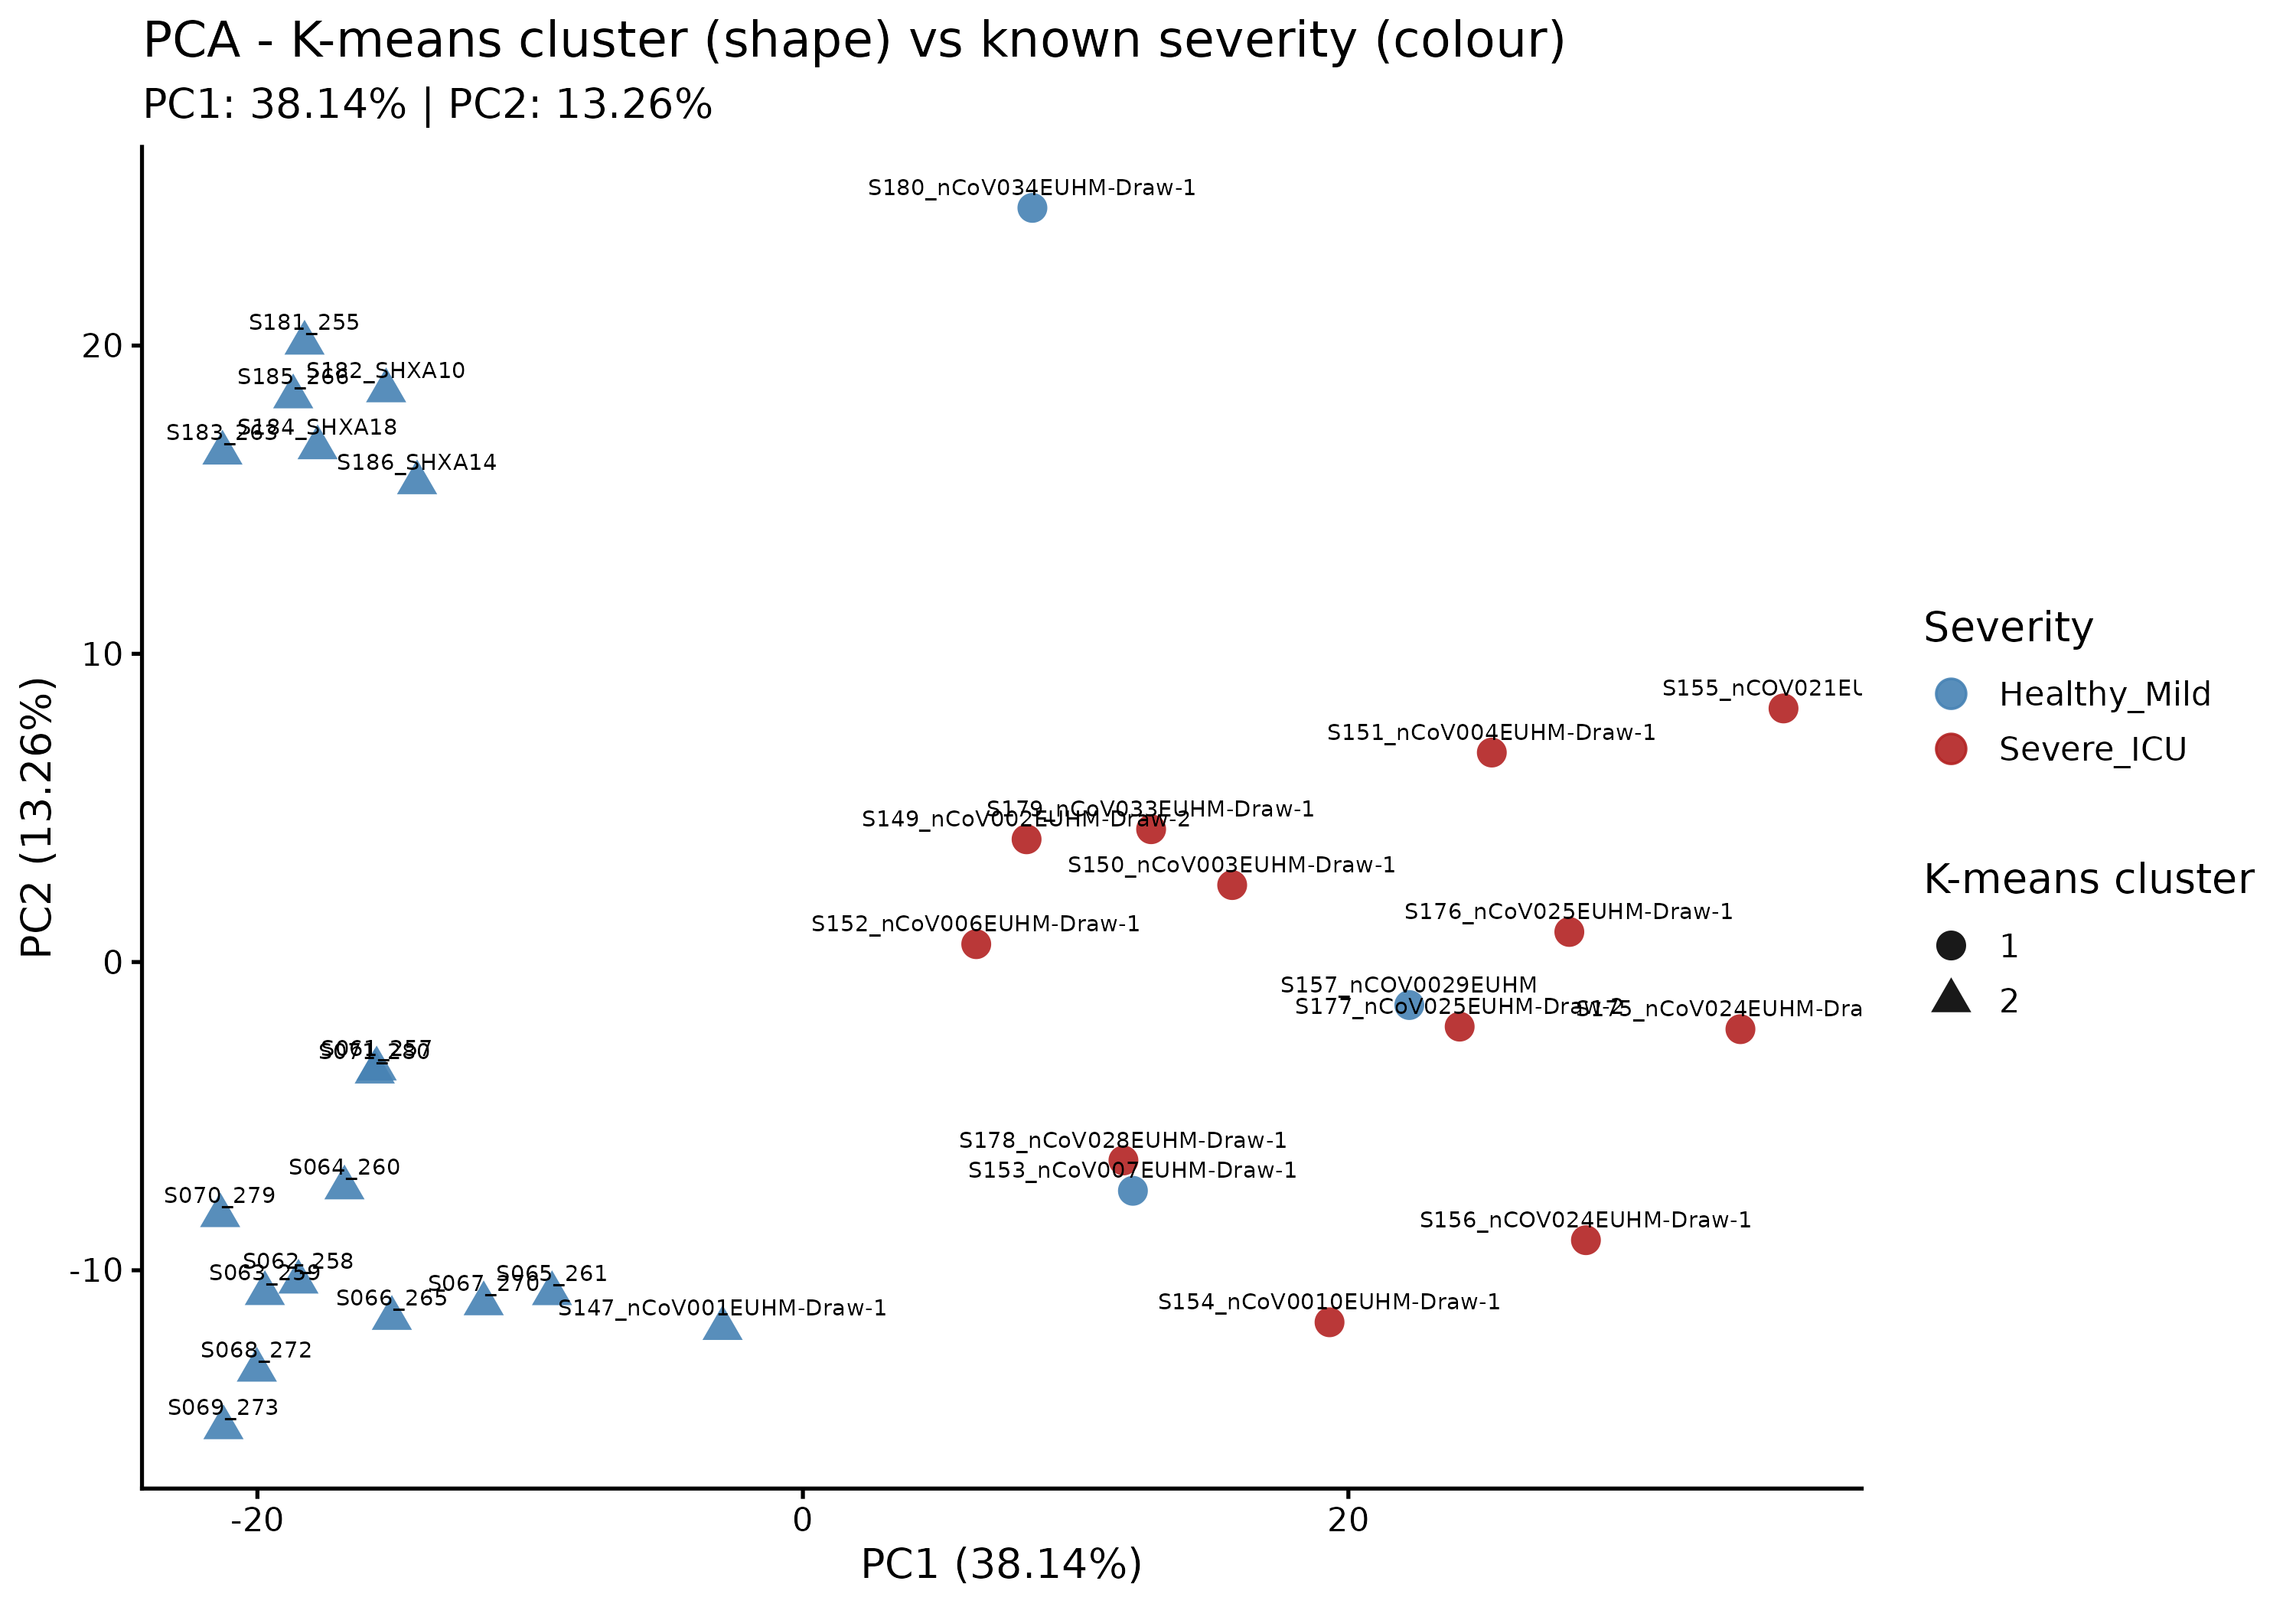
\includegraphics[width=0.9\textwidth]{plots/phase11/phase11_PCA_kmeans_overlay.png}
\end{center}

Colour = known severity label; shape = k-means cluster assignment.
A perfect match appears as all circles (cluster 1) being red and all triangles
(cluster 2) being blue.

\begin{itemize}[nosep]
  \item All blue (Healthy) dots are triangles (cluster 2) — \textbf{perfect recovery}
        of the entire Healthy/Mild group.
  \item All red (Severe) dots are circles (cluster 1) — \textbf{except}
        S147\_nCoV001EUHM-Draw-1, which is a red dot with a triangle shape: the
        same Severe outlier that hierarchical clustering also misclassified.
  \item \textbf{K-means accuracy: 32/33 (97\%)} — identical to the hierarchical result.
        Two independent algorithms with completely different logic flag the same single
        outlier and agree on every other sample.
\end{itemize}

\subsection{Phase 11 conclusion}

Phase 11 confirms that the DE gene signal from Phases 8--9 is not a statistical
artefact — it is a pervasive, whole-transcriptome difference that reorganises samples
into two groups on its own, without any label input.

\begin{enumerate}[nosep]
  \item \textbf{PC1 (38\% of variance) captures severity completely.}
        Every Healthy/Mild sample has negative PC1; every Severe/ICU sample has
        positive PC1. No overlap. A single axis in gene expression space encodes
        whether a patient is severely ill.

  \item \textbf{Gender has no visible effect in the PCA.}
        Females and males are intermixed within each severity group on every PC axis.
        This is the visual complement to the $r = 0.97$ model comparison in Phase 9.

  \item \textbf{Both the correlation and distance matrices show a clean two-block
        structure.} Within-group similarity is high; between-group similarity is low.
        The boundary is sharp and consistent.

  \item \textbf{Hierarchical clustering and k-means independently recover the two
        groups with 97\% accuracy.}
        The elbow at $k = 2$ confirms two is the natural number of clusters.
        Both algorithms flag the exact same single outlier.

  \item \textbf{One Severe sample (S147\_nCoV001EUHM-Draw-1) is a genuine outlier.}
        Its transcriptome looks more like Healthy than Severe, flagged by both
        algorithms independently. It likely represents a Severe patient at an
        atypical disease stage or with an unusual immune response.
\end{enumerate}

\textbf{What this means for the story:}
The bulk transcriptome of severe COVID blood is categorically different from
healthy blood — not just at individual genes, but across the whole expression
profile. The structure is strong enough that a simple algorithm with no prior
knowledge of which samples are sick can sort them with near-perfect accuracy.
This sets the stage for Phase 12, which asks:
\textit{what biological programs and pathways drive this difference?}

% ─────────────────────────────────────────────────────────
\subsection{GSEA — testing whole programs instead of individual genes}

Phases 8--10 asked which \textit{individual genes} change.
GSEA asks a different question: does a predefined \textit{set of genes}
that together form a biological program change as a whole?

\subsubsection*{The simple idea}

You have a list of all genes, ranked from most upregulated in Severe
to most downregulated. You pick a gene set — say, all TNF/NF-$\kappa$B
target genes. GSEA walks down the ranked list and checks:
are the TNF target genes clustering at the top (activated in Severe),
at the bottom (suppressed in Severe), or randomly spread out (no change)?

The result is a \textbf{normalized enrichment score (NES)}:
\begin{itemize}[nosep]
  \item \textbf{Positive NES} — genes in this set are concentrated near the
        top of the ranked list. The program is activated in Severe.
  \item \textbf{Negative NES} — genes are concentrated near the bottom.
        The program is suppressed in Severe.
\end{itemize}

\subsubsection*{Why GSEA instead of just looking at the gene list?}

A gene set can be ``active'' even if no single gene in it individually
passes the fold-change or p-value cutoff. If 80 genes all move slightly
in the same direction, GSEA detects the coordinated shift; a gene-by-gene
approach misses it because no single gene is extreme enough.
This makes GSEA more sensitive for detecting broad biological programs.

\subsubsection*{The four databases used}

\begin{itemize}[nosep]
  \item \textbf{GO:BP} (Gene Ontology Biological Process) — broad
        biological processes defined by gene function annotation.
  \item \textbf{Hallmark} (MSigDB) — 50 curated programs defining
        the most coherent, well-studied biological states.
  \item \textbf{KEGG} — metabolic and signaling pathways.
  \item \textbf{Reactome} — detailed molecular reaction pathways.
\end{itemize}

Using four databases cross-validates that findings are robust and not
specific to one annotation system.

% ─────────────────────────────────────────────
\section{Phase 12 — GSEA Pathway Analysis}
% ─────────────────────────────────────────────

\subsection{Phase 12 overview — the big picture}

\textbf{Phase 11 confirmed that samples separate by severity. Phase 12 asks:
what biological programs explain that separation?}

Instead of asking ``which genes change?'', we now ask
``which biological processes change as programs?''
The DE gene list from Phase 9 (gender-adjusted model) is ranked by
fold-change and fed into GSEA against four gene-set databases.
The result is a map of which programs are switched on and switched off
in severe COVID blood — at the pathway level.

\subsection{GO Biological Process \small\normalfont\textit{(gobp\_dotplot)}}

\begin{center}
  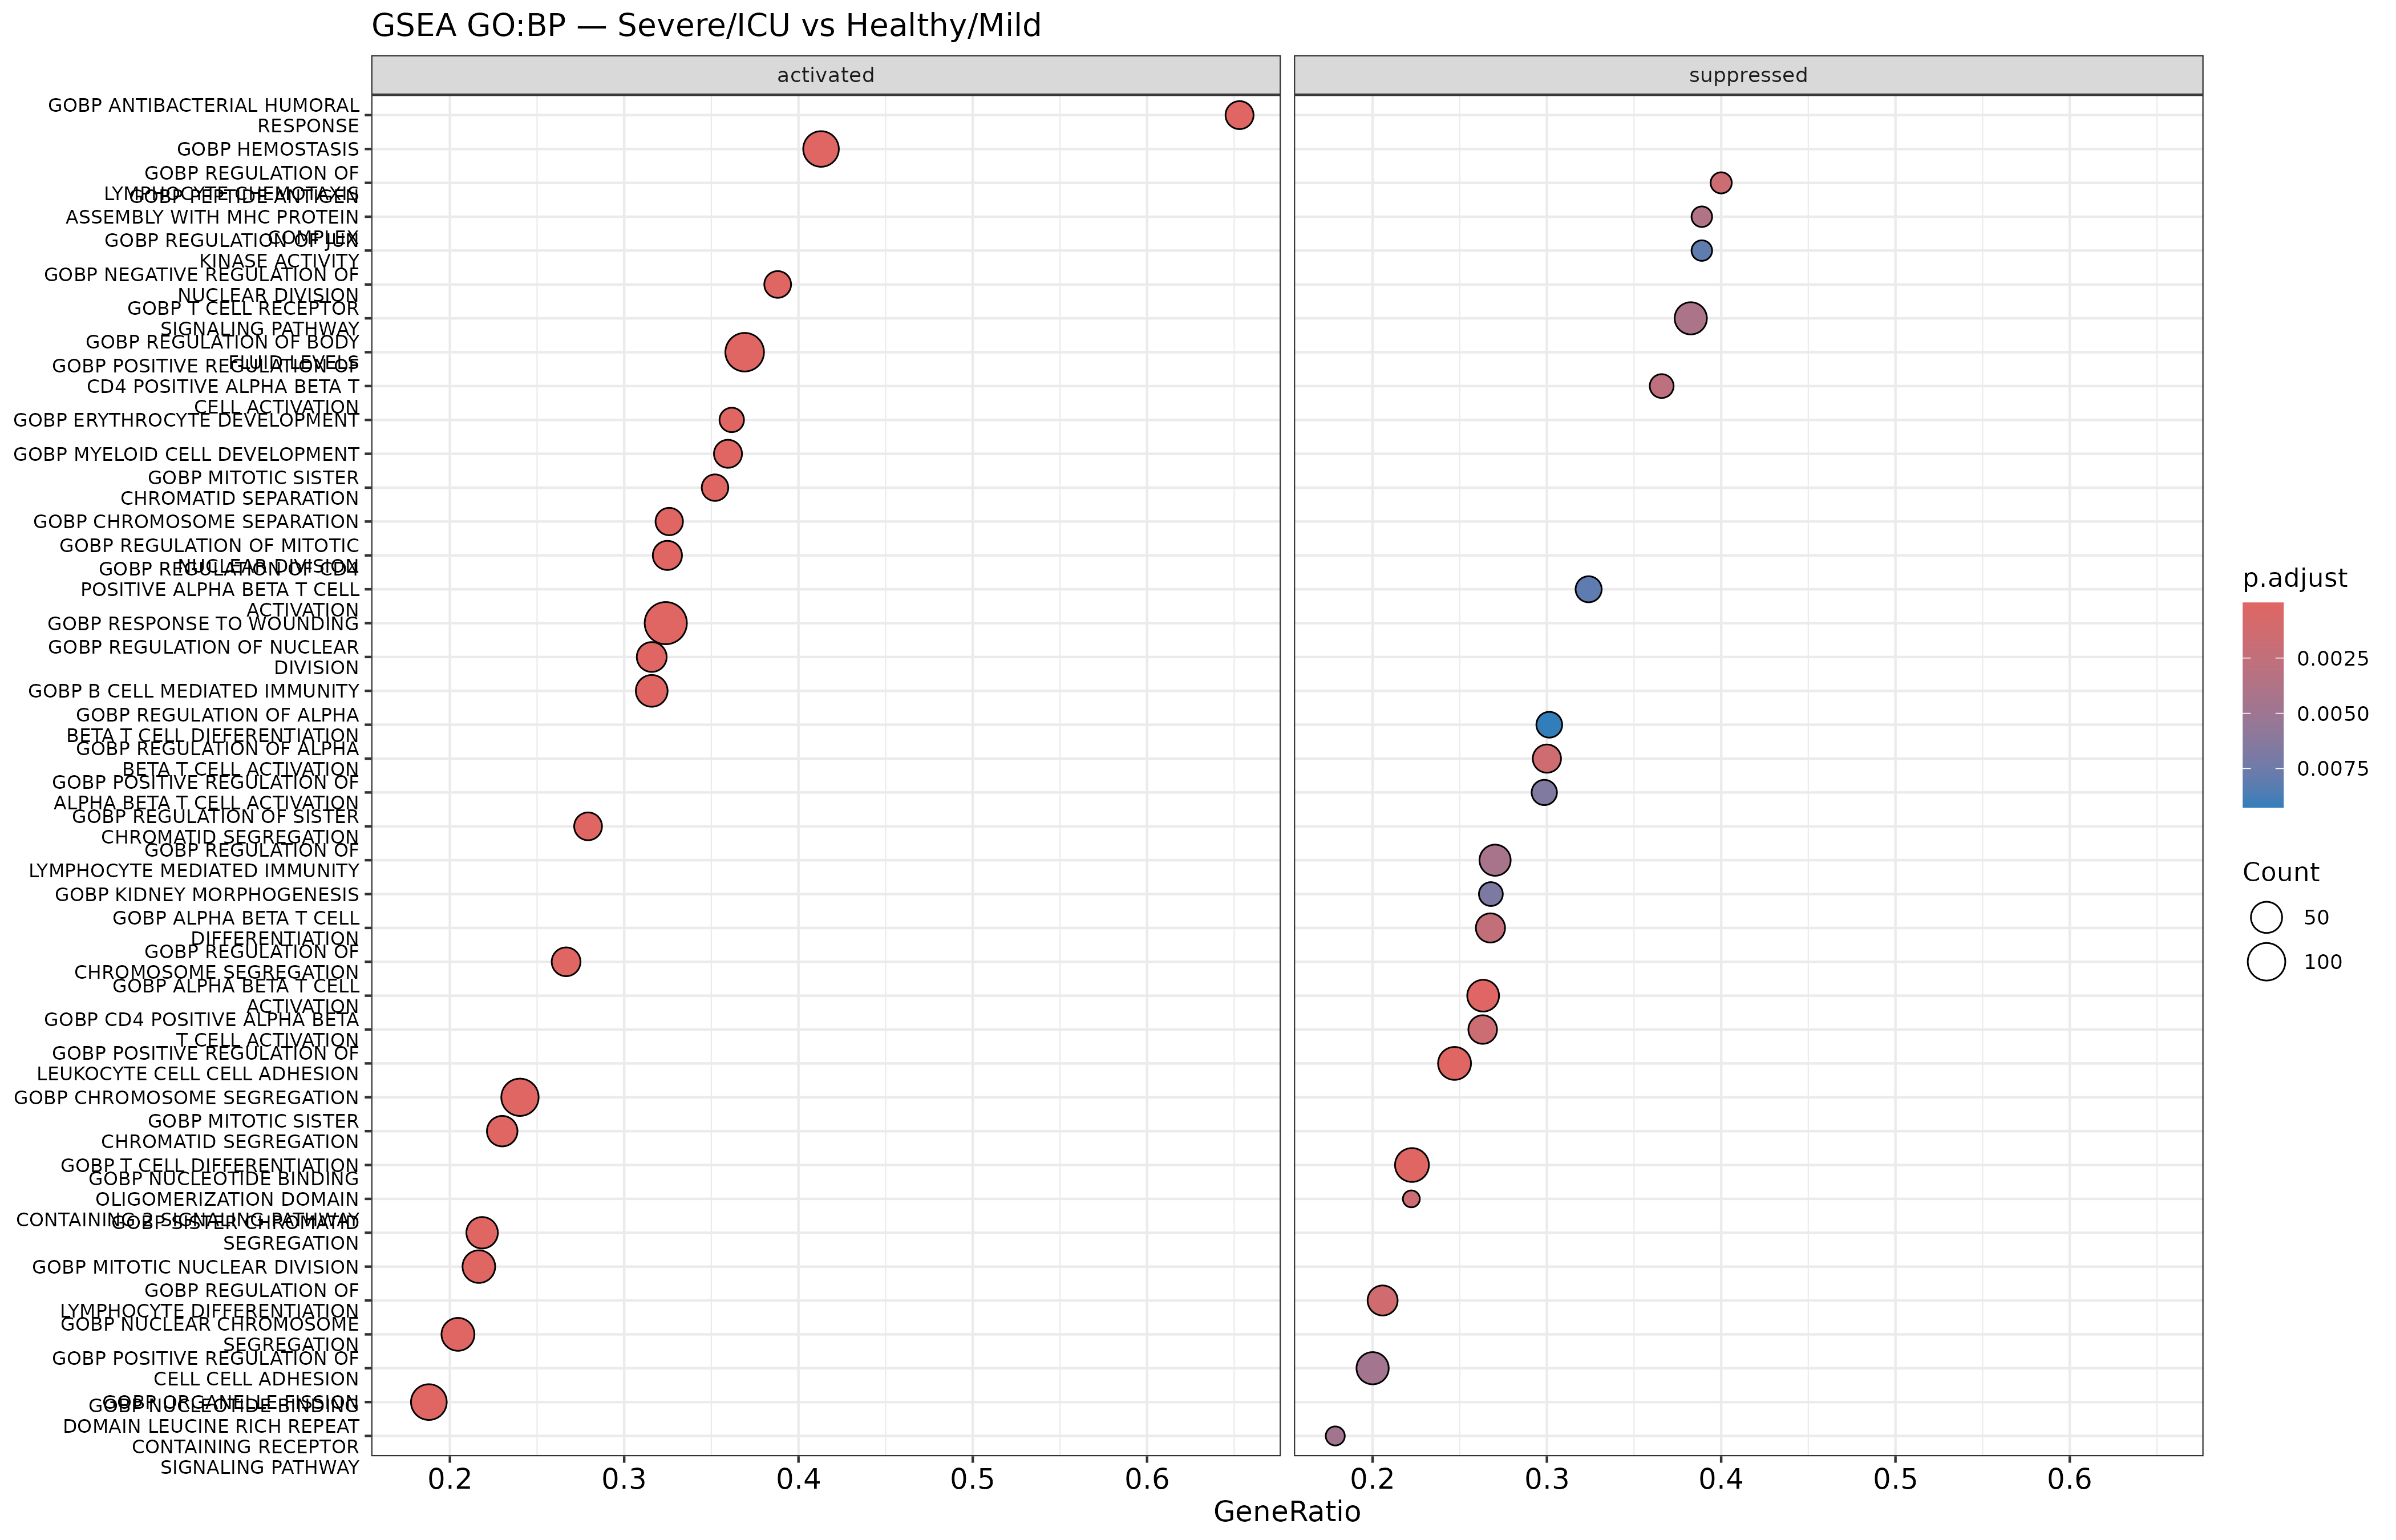
\includegraphics[width=\textwidth]{plots/phase12/phase12_gobp_dotplot.png}
\end{center}

Dot size = number of genes in the set that contributed to enrichment;
colour = adjusted p-value (red = more significant);
x-axis = GeneRatio (fraction of the gene set found in the ranked list).
Left panel = activated in Severe; right panel = suppressed in Severe.

\textit{Activated programs (left):}
\begin{itemize}[nosep]
  \item \textbf{GOBP Antibacterial Humoral Response (GeneRatio $\approx$ 0.65)} —
        the single most activated GO term. This covers complement proteins, coagulation
        factors, and antimicrobial peptides secreted into the blood.
        Its top position is driven by the platelet and coagulation gene expansion
        documented in Phase 8.
  \item \textbf{GOBP Hemostasis ($\approx$ 0.40)} — blood clotting and coagulation.
        Consistent with the SELP, ITGA2B, PROS1, and F13A1 upregulation from Phase 8.
        Thrombotic complications are a hallmark of severe COVID-19.
  \item \textbf{GOBP Myeloid Cell Development ($\approx$ 0.28)} and
        \textbf{Erythrocyte Development ($\approx$ 0.27)} — emergency myelopoiesis:
        the bone marrow pushing out immature myeloid cells and red-blood-cell precursors
        under the stress of severe infection.
  \item \textbf{Mitotic chromosome segregation terms ($\approx$ 0.20--0.25)} —
        cell division activity, consistent with the proliferating monocyte
        precursor cluster (Cluster 15) seen in Phase 3.
\end{itemize}

\textit{Suppressed programs (right):}
\begin{itemize}[nosep]
  \item \textbf{CD4-Positive Alpha-Beta T Cell Activation ($\approx$ 0.40)} and
        related T cell terms — the most significantly suppressed GO terms.
        The GO analysis recovers the CD4$^+$ T cell depletion from Phase 4 as a
        pathway-level finding: not just individual T cell genes are lost, but the
        entire CD4$^+$ T cell activation program is turned off in bulk blood.
  \item \textbf{GOBP Lymphocyte Differentiation and Mediated Immunity} —
        B cell and T cell adaptive immunity programs broadly reduced.
  \item \textbf{GOBP Complement Complex Assembly with MHC Protein} —
        antigen-presentation linked terms are suppressed, echoing the
        HLA downregulation seen in the Phase 4 volcano.
\end{itemize}

\textbf{Summary:} GO:BP frames the severity difference as innate immunity
taking over (myeloid expansion, hemostasis, antibacterial) while adaptive
immunity retreats (T cell, B cell, MHC programs suppressed).

\subsection{Hallmark gene sets \small\normalfont\textit{(hallmark\_dotplot)}}

\begin{center}
  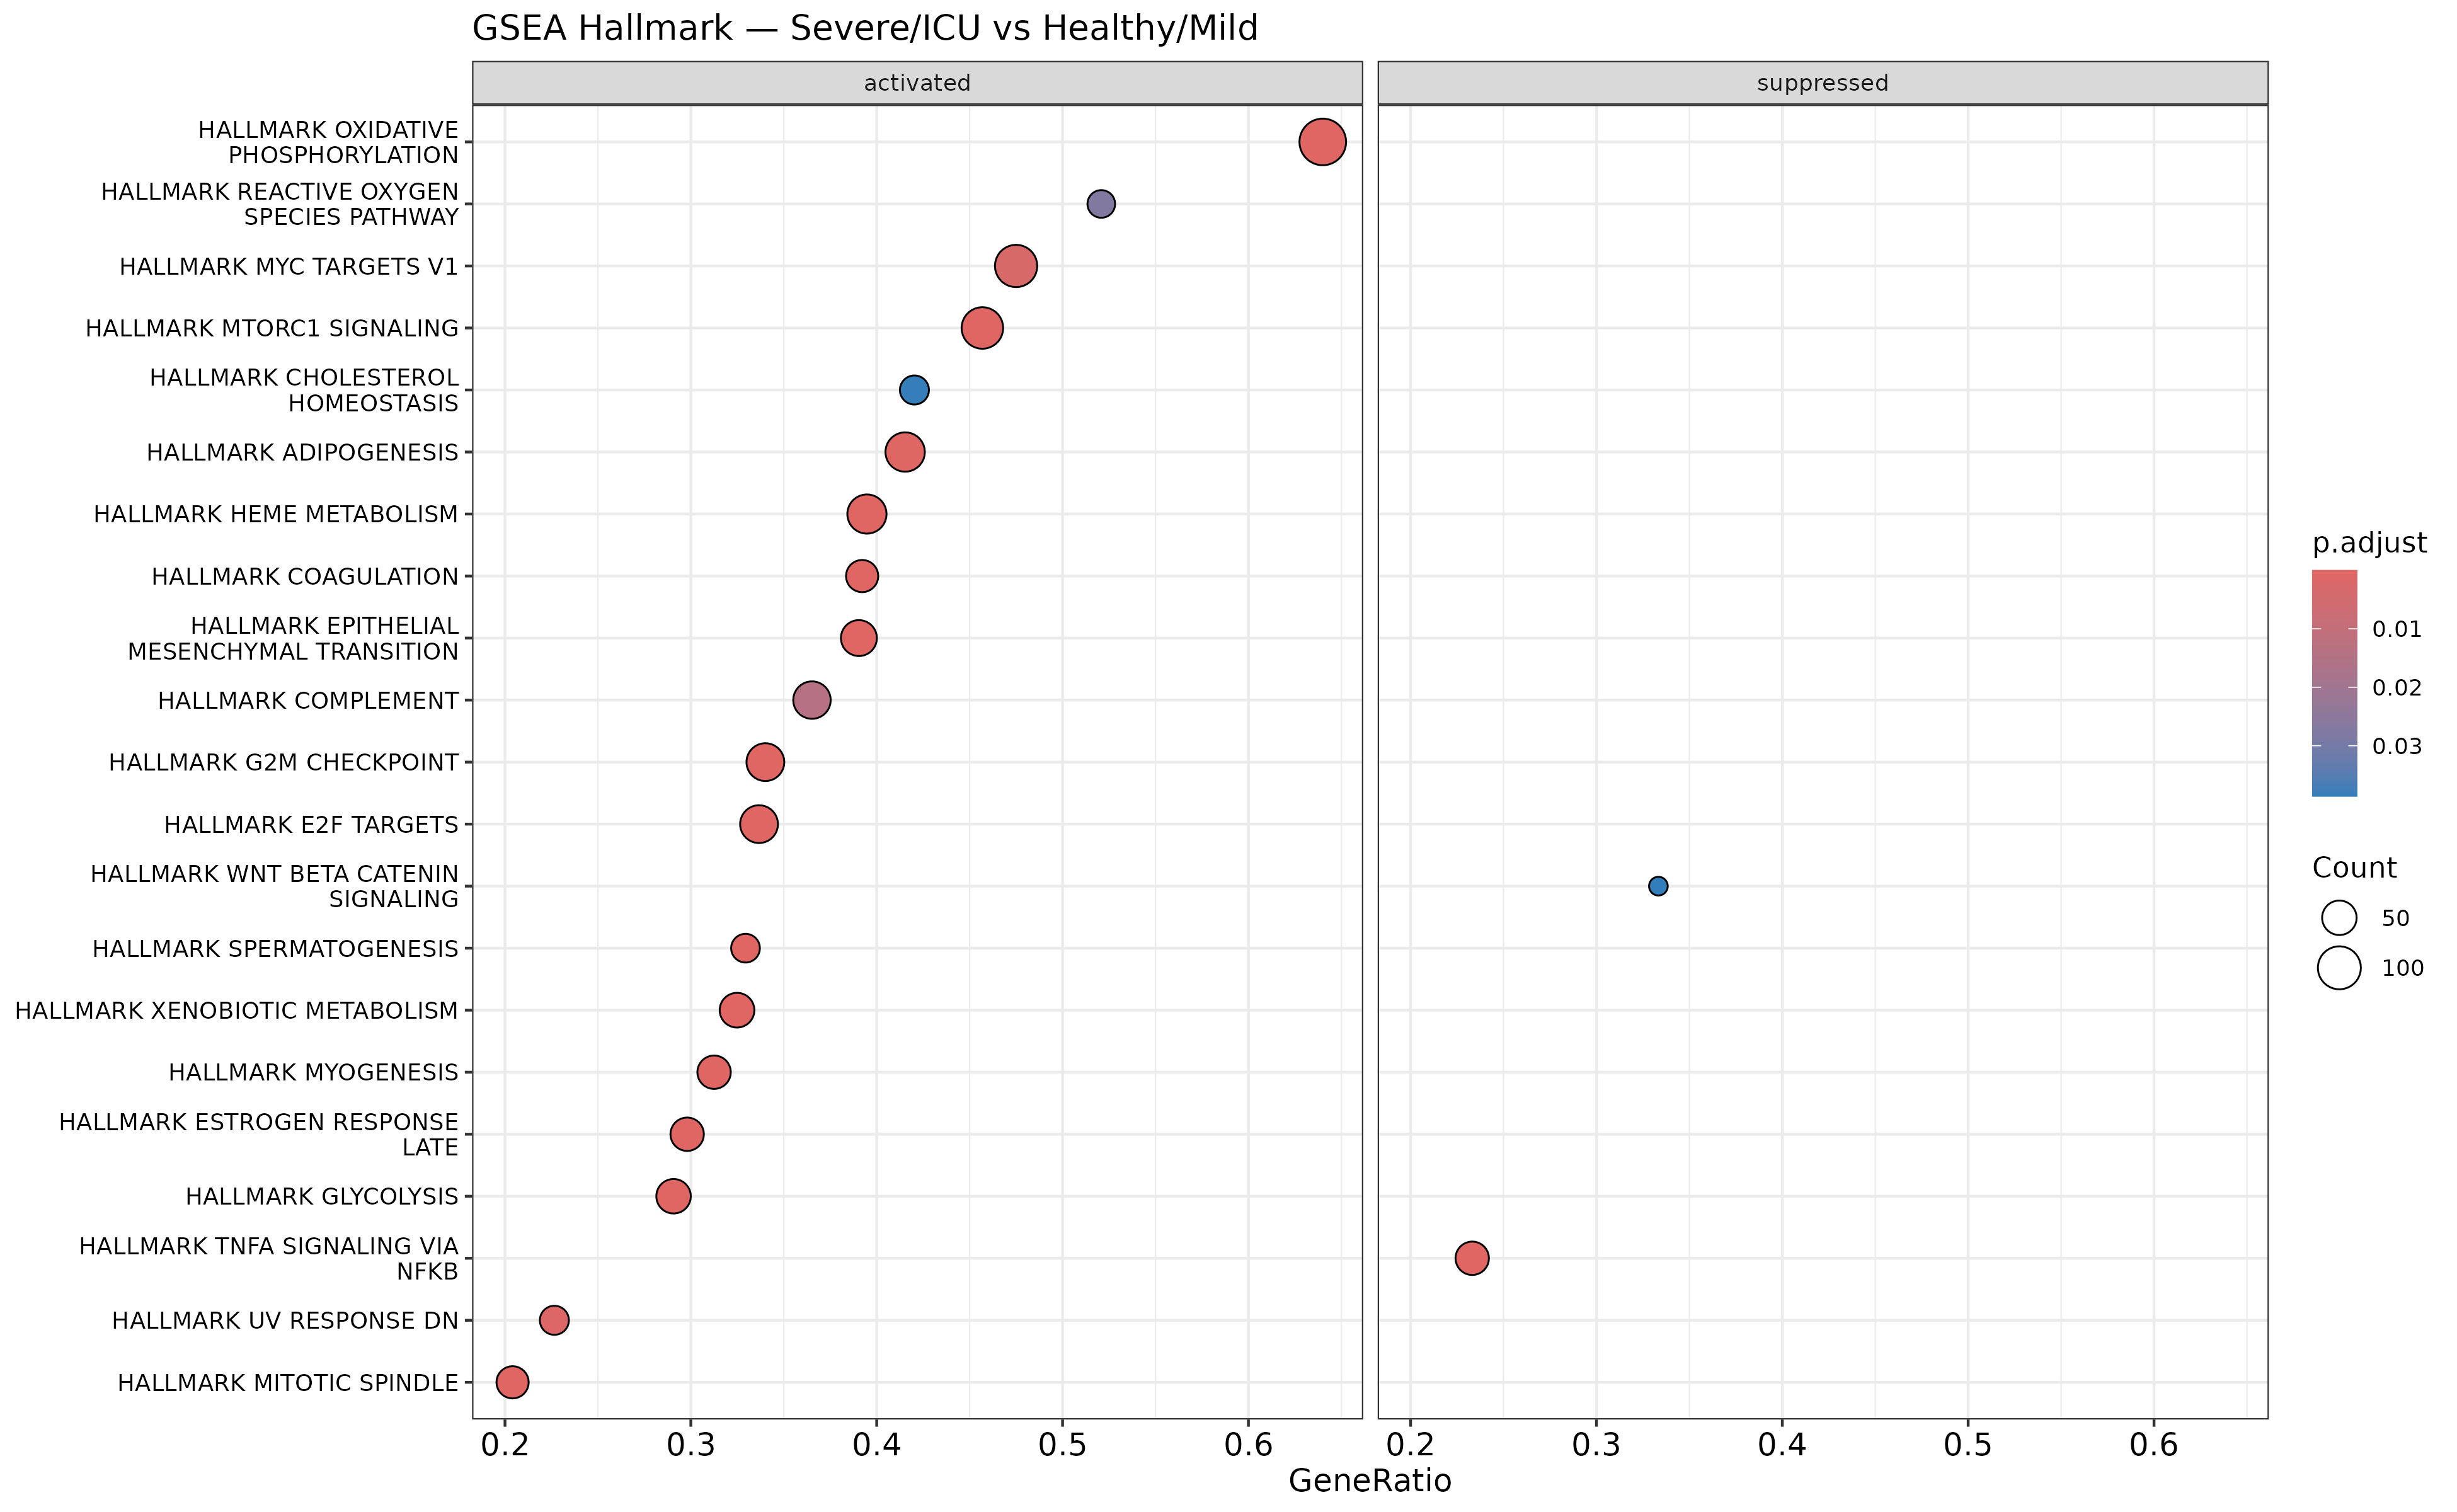
\includegraphics[width=0.95\textwidth]{plots/phase12/phase12_hallmark_dotplot.png}
\end{center}

The Hallmark collection contains 50 curated programs representing the most
well-characterized biological states. Fewer but more interpretable results.

\textit{Activated programs:}
\begin{itemize}[nosep]
  \item \textbf{HALLMARK Oxidative Phosphorylation (GeneRatio $\approx$ 0.65)} —
        the most strongly activated Hallmark program by a wide margin.
        Oxidative phosphorylation (OxPhos) is the mitochondrial process that
        generates ATP. Its activation in severe COVID blood reflects two things:
        (1) expanded platelets and monocytes are metabolically active cells
        with high mitochondrial activity; (2) severe disease drives a metabolic
        reprogramming in immune cells from aerobic glycolysis toward mitochondrial
        respiration.
  \item \textbf{HALLMARK Reactive Oxygen Species Pathway ($\approx$ 0.52)} —
        ROS production, directly connected to OxPhos activity.
        Together, these two terms indicate \textbf{mitochondrial stress} in the
        expanded myeloid/platelet population.
  \item \textbf{HALLMARK MYC Targets V1 ($\approx$ 0.47)} and
        \textbf{mTORC1 Signaling ($\approx$ 0.43)} — two master growth and
        proliferation regulators switched on. Their activation is consistent
        with emergency myelopoiesis: cells that are actively proliferating need
        MYC and mTORC1 to drive biosynthesis.
  \item \textbf{HALLMARK Coagulation ($\approx$ 0.37)} — confirms the
        hemostasis finding from GO:BP and the individual coagulation gene
        upregulation from Phase 8.
  \item \textbf{HALLMARK Complement ($\approx$ 0.35)} — the complement cascade
        is a key innate immune effector; its activation is expected and consistent
        with the antibacterial humoral response term from GO:BP.
  \item \textbf{HALLMARK G2M Checkpoint ($\approx$ 0.33)} and
        \textbf{E2F Targets ($\approx$ 0.30)} — DNA replication and cell cycle
        programs activated, again consistent with proliferating immune progenitors.
\end{itemize}

\textit{Suppressed programs:}
\begin{itemize}[nosep]
  \item \textbf{HALLMARK TNF$\alpha$ Signaling via NF-$\kappa$B (GeneRatio $\approx$ 0.25)} —
        \textbf{this is the most important finding in Phase 12.}
        The TNF/NF-$\kappa$B program — the same inflammatory program that was strongly
        upregulated in monocytes in Phase 4 — is \textit{suppressed in bulk blood}.
        This is the definitive bulk-level confirmation of the dilution paradox:
        TNF and its downstream targets are produced by T cells, NK cells, and B cells
        that are all depleted in severe COVID. Their loss outweighs the gain from monocytes.
  \item \textbf{HALLMARK WNT/Beta-Catenin Signaling} — a lymphoid differentiation
        pathway, suppressed with lymphocyte depletion.
\end{itemize}

\subsection{TNF/NF-$\kappa$B GSEA enrichment plot}

\begin{center}
  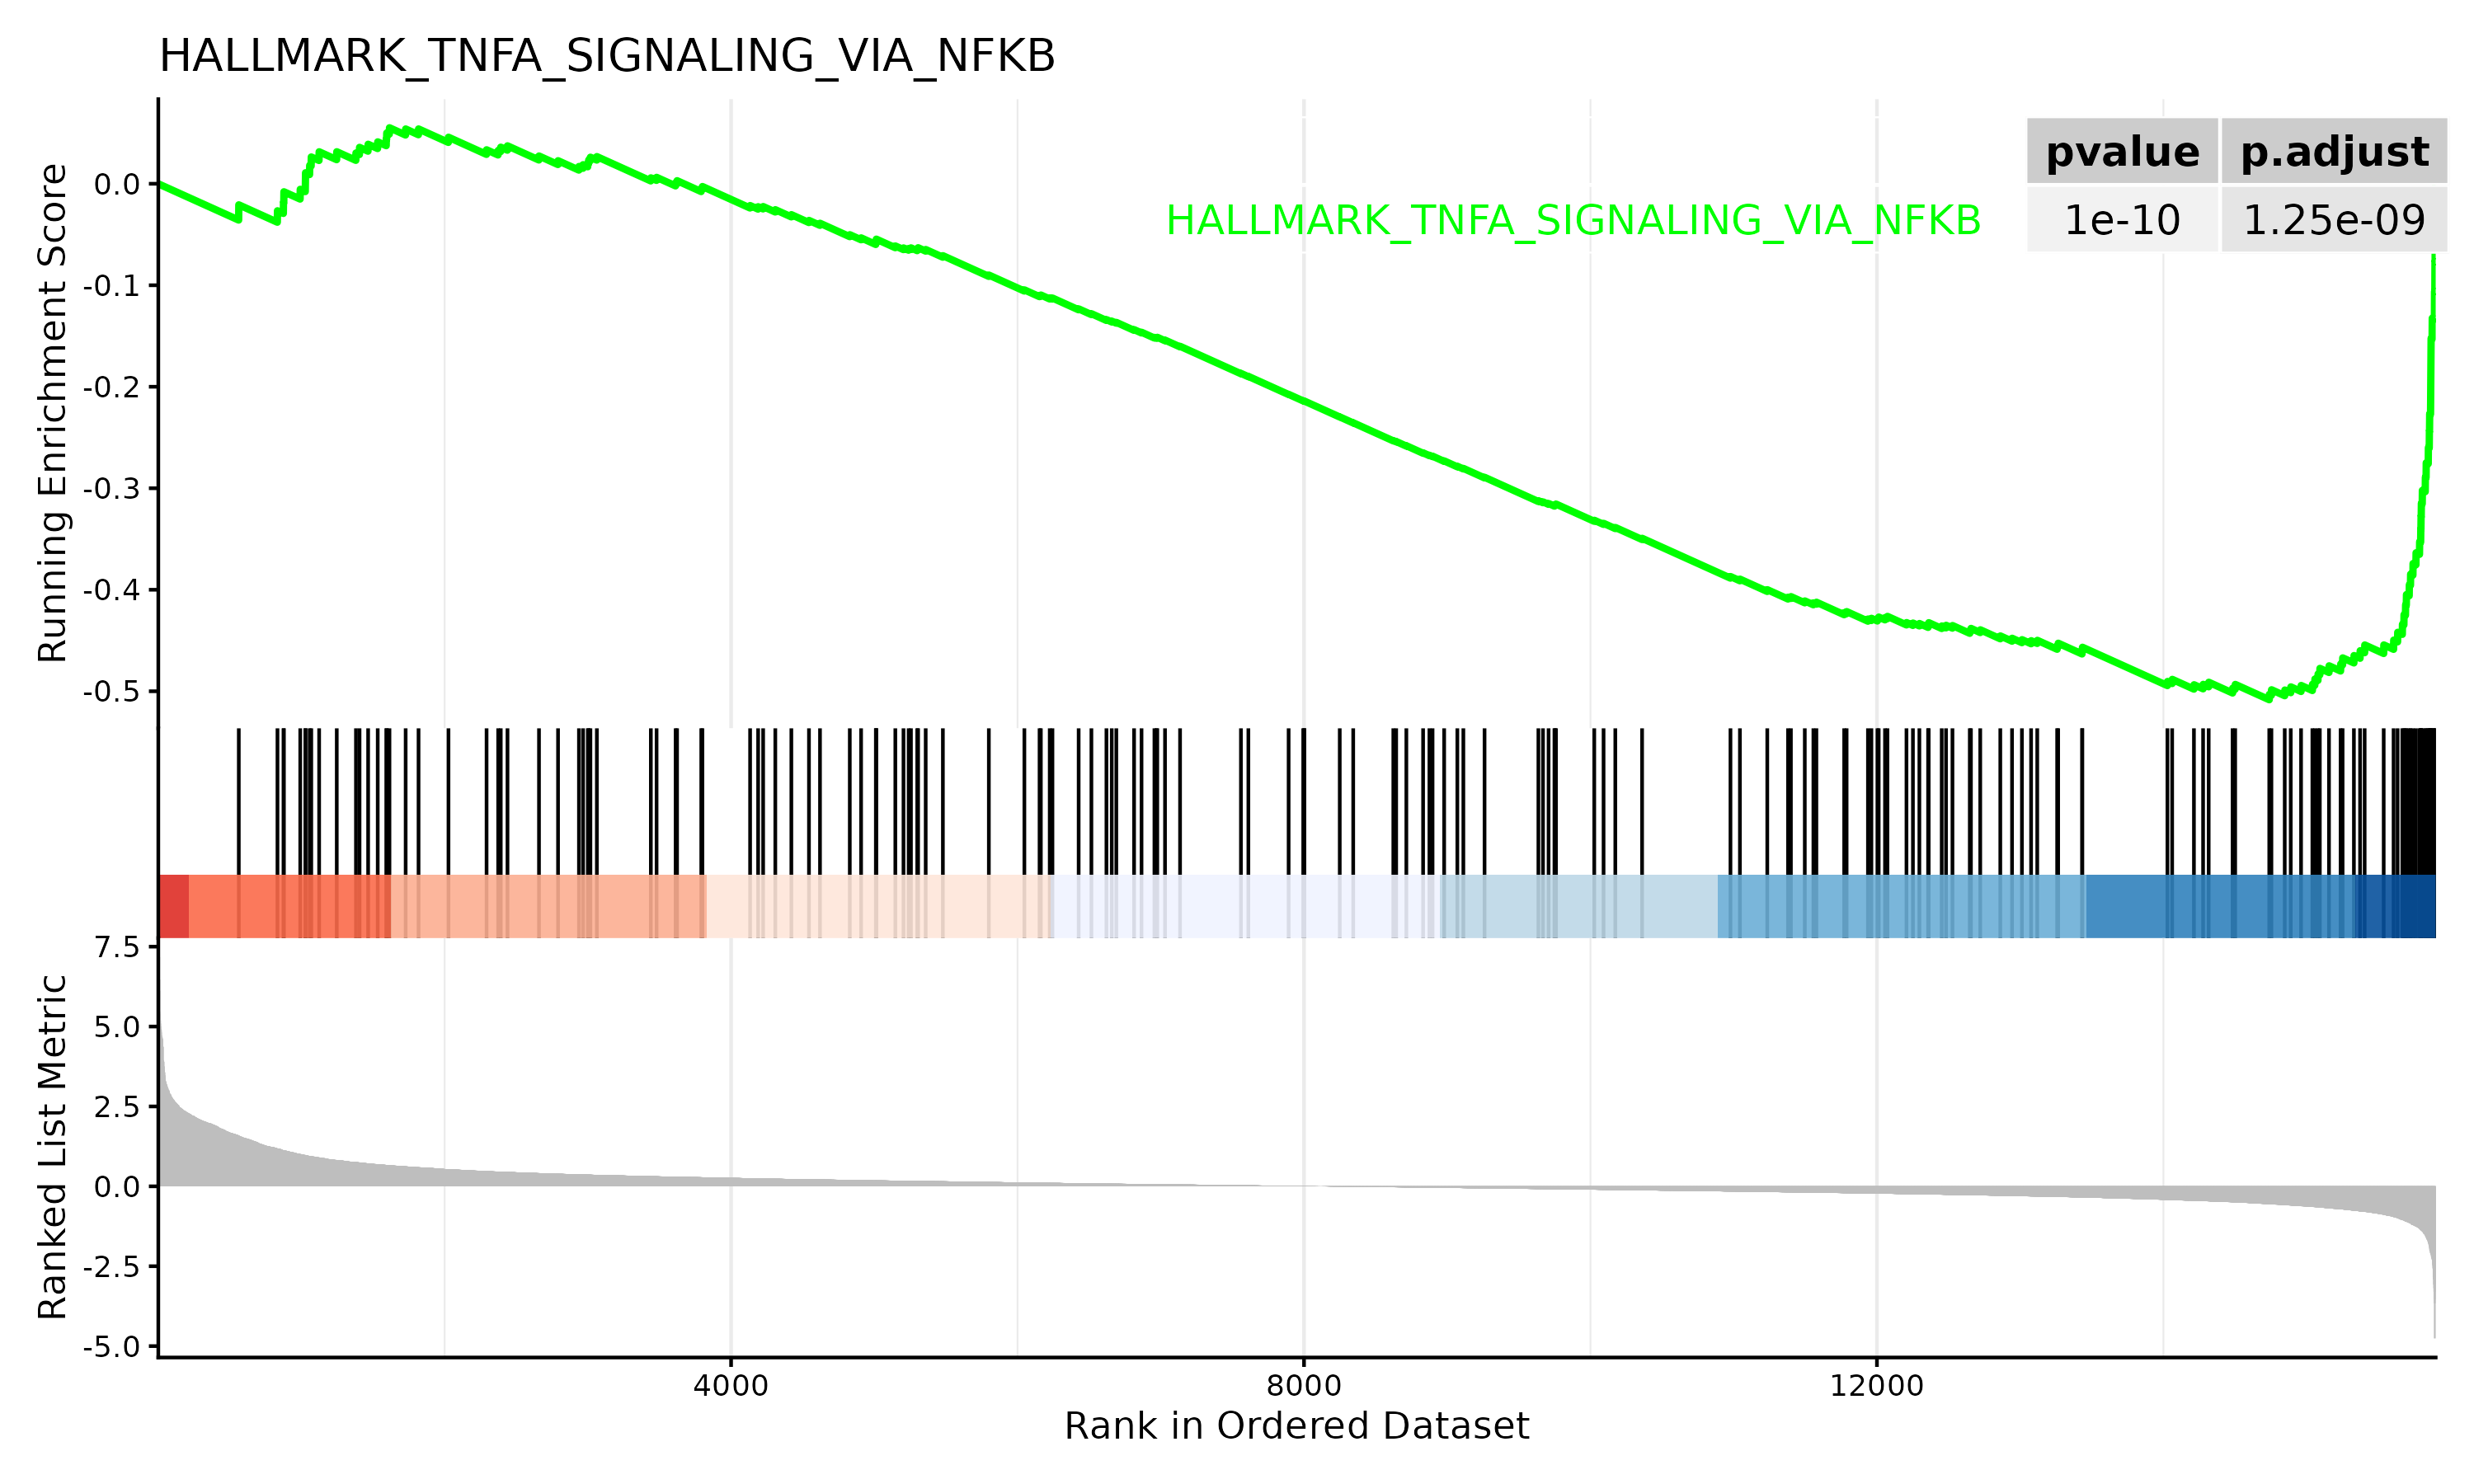
\includegraphics[width=0.9\textwidth]{plots/phase12/phase12_gsea_TNF_NFKB.png}
\end{center}

This is the classic GSEA running enrichment score (RES) plot for
HALLMARK\_TNFA\_SIGNALING\_VIA\_NFKB.

\textbf{How to read it:}
The x-axis is the full gene list, sorted from most upregulated in Severe (left)
to most downregulated (right). The green curve tracks the running enrichment score
as you walk down the list: it rises when you encounter a gene in the set,
and falls when you don't. The tick marks in the middle are the positions of
the TNF/NF-$\kappa$B genes in the ranked list.
The coloured bar below shows the fold-change magnitude: red = upregulated in Severe;
blue = downregulated.

\textbf{What the plot shows:}
\begin{itemize}[nosep]
  \item The green curve immediately dips below zero and continues falling
        steadily all the way to about $-0.5$ near rank $\sim$13,000.
        This means there are essentially \textbf{no TNF/NF-$\kappa$B genes in the
        upregulated half of the ranked list}.
  \item The tick marks are \textbf{densely clustered at the far right} (downregulated
        end) — the TNF/NF-$\kappa$B genes are preferentially in the genes most
        downregulated in Severe COVID.
  \item The sharp spike back up at the very end ($\sim$rank 14,000) shows the
        concentration of gene hits at the downregulated tail.
  \item \textbf{p-value = $10^{-10}$, padj = $1.25 \times 10^{-9}$} — extremely
        significant suppression.
\end{itemize}

This plot is the single most important result of Phase 12 for the project story.
It directly and unambiguously shows that the TNF/NF-$\kappa$B inflammatory program —
central to the co-activation hypothesis — is a \textbf{net loss} in severe COVID
\textit{blood}, not a gain. The individual gene upregulation in monocytes (Phase 4)
is completely invisible at the bulk level, buried under the much larger signal of
lymphocyte loss.

\subsection{KEGG pathways \small\normalfont\textit{(kegg\_dotplot)}}

\begin{center}
  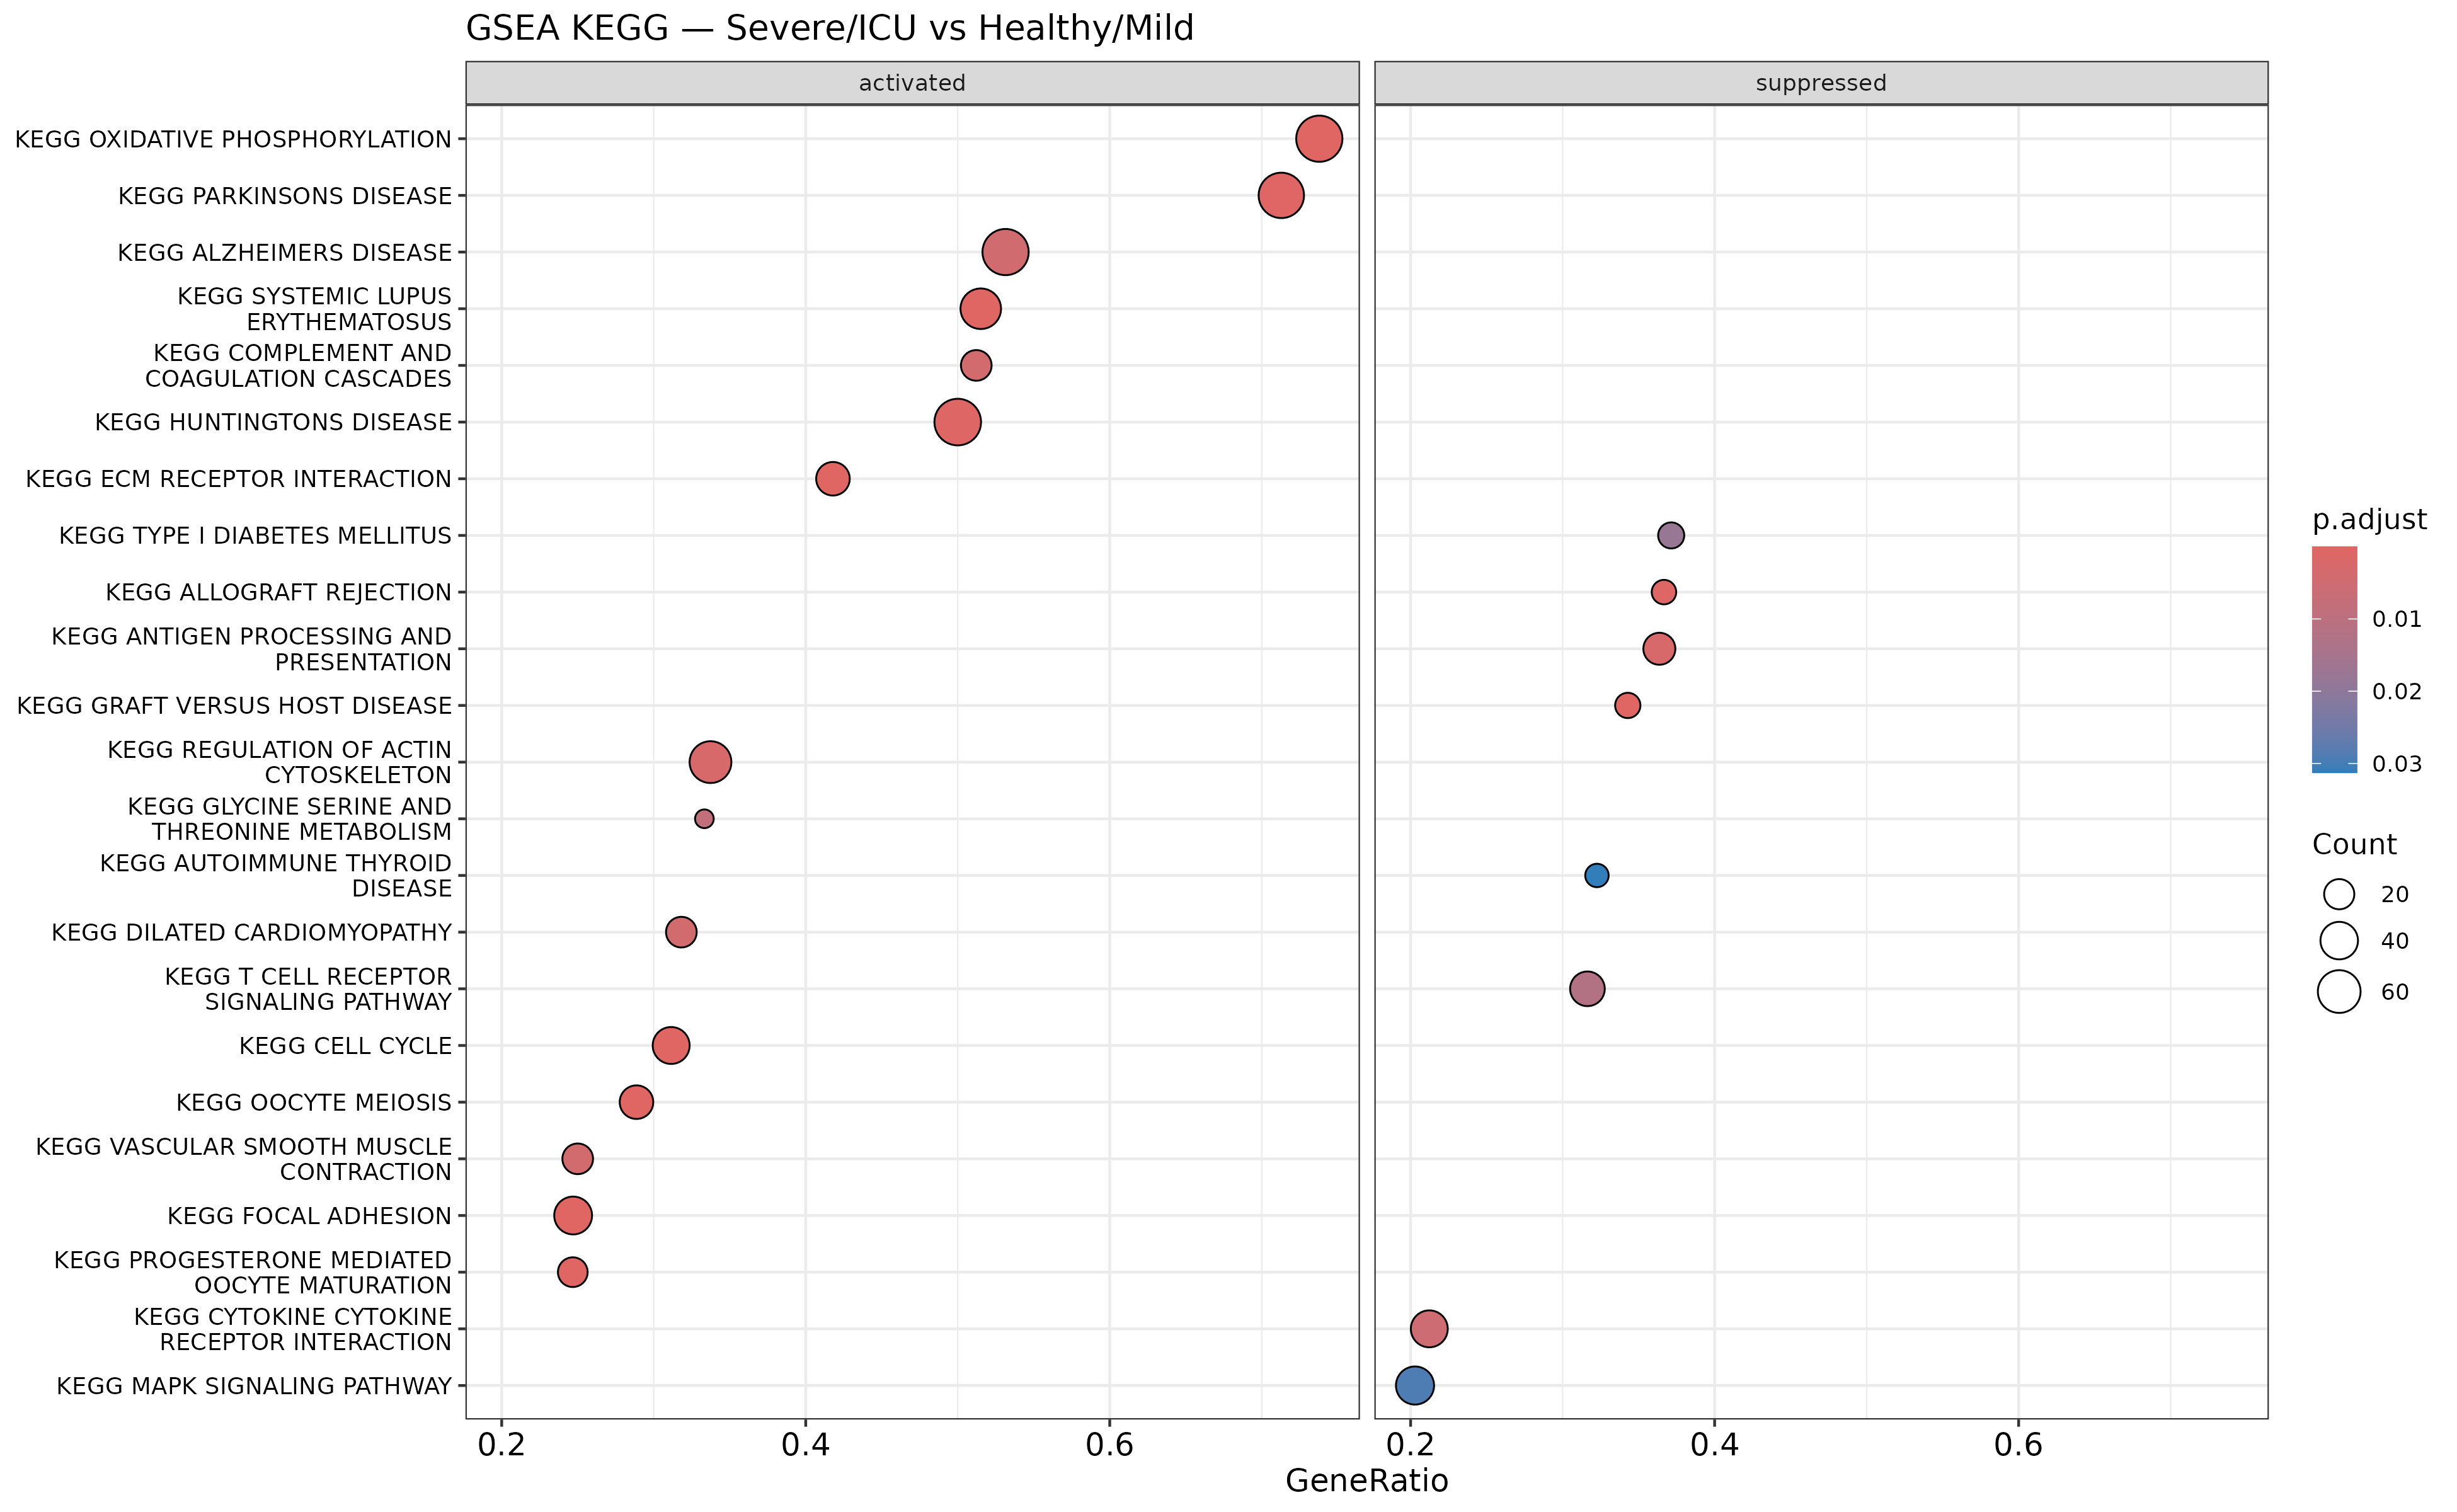
\includegraphics[width=0.95\textwidth]{plots/phase12/phase12_kegg_dotplot.png}
\end{center}

\textit{Activated:}
\begin{itemize}[nosep]
  \item \textbf{KEGG Oxidative Phosphorylation ($\approx$ 0.68)} — the top KEGG
        term, consistent with the Hallmark OxPhos result.
  \item \textbf{KEGG Parkinson's Disease ($\approx$ 0.65), Alzheimer's Disease
        ($\approx$ 0.48), Huntington's Disease ($\approx$ 0.42)} — these appear
        activated, which might seem alarming. They are \textit{not} meaningful:
        these KEGG pathways all contain large blocks of mitochondrial complex genes
        (Complex I, II, III, IV) that overlap nearly completely with the OxPhos gene
        set. It is the same OxPhos signal appearing under multiple pathway labels.
        This is a known KEGG annotation artefact.
  \item \textbf{KEGG Complement and Coagulation Cascades ($\approx$ 0.44)} —
        a direct and biologically meaningful result; consistent across all four databases.
  \item \textbf{KEGG Systemic Lupus Erythematosus ($\approx$ 0.46)} — appears
        because this KEGG set includes many complement and chromatin/histone genes;
        the complement portion drives the enrichment.
  \item \textbf{KEGG Cell Cycle ($\approx$ 0.31)} — proliferating myeloid progenitor
        signal, consistent with MYC/mTORC1 from Hallmark.
\end{itemize}

\textit{Suppressed:}
\begin{itemize}[nosep]
  \item \textbf{KEGG Antigen Processing and Presentation ($\approx$ 0.35)} —
        directly reflects HLA class II downregulation seen in Phase 4 and the
        lymphocyte depletion. The cell machinery that shows foreign peptides to
        T cells is globally reduced.
  \item \textbf{KEGG Allograft Rejection ($\approx$ 0.32) and Graft-vs-Host
        Disease ($\approx$ 0.30)} — both contain T cell activation and HLA genes;
        suppressed as expected with T cell loss.
  \item \textbf{KEGG T Cell Receptor Signaling Pathway ($\approx$ 0.30)} —
        direct evidence that T cell signaling is globally shut down in severe
        COVID blood.
  \item \textbf{KEGG Cytokine-Cytokine Receptor Interaction ($\approx$ 0.21)
        and MAPK Signaling Pathway} — general immune signaling suppressed,
        driven by lymphocyte depletion.
\end{itemize}

\subsection{Reactome pathways \small\normalfont\textit{(reactome\_dotplot)}}

\begin{center}
  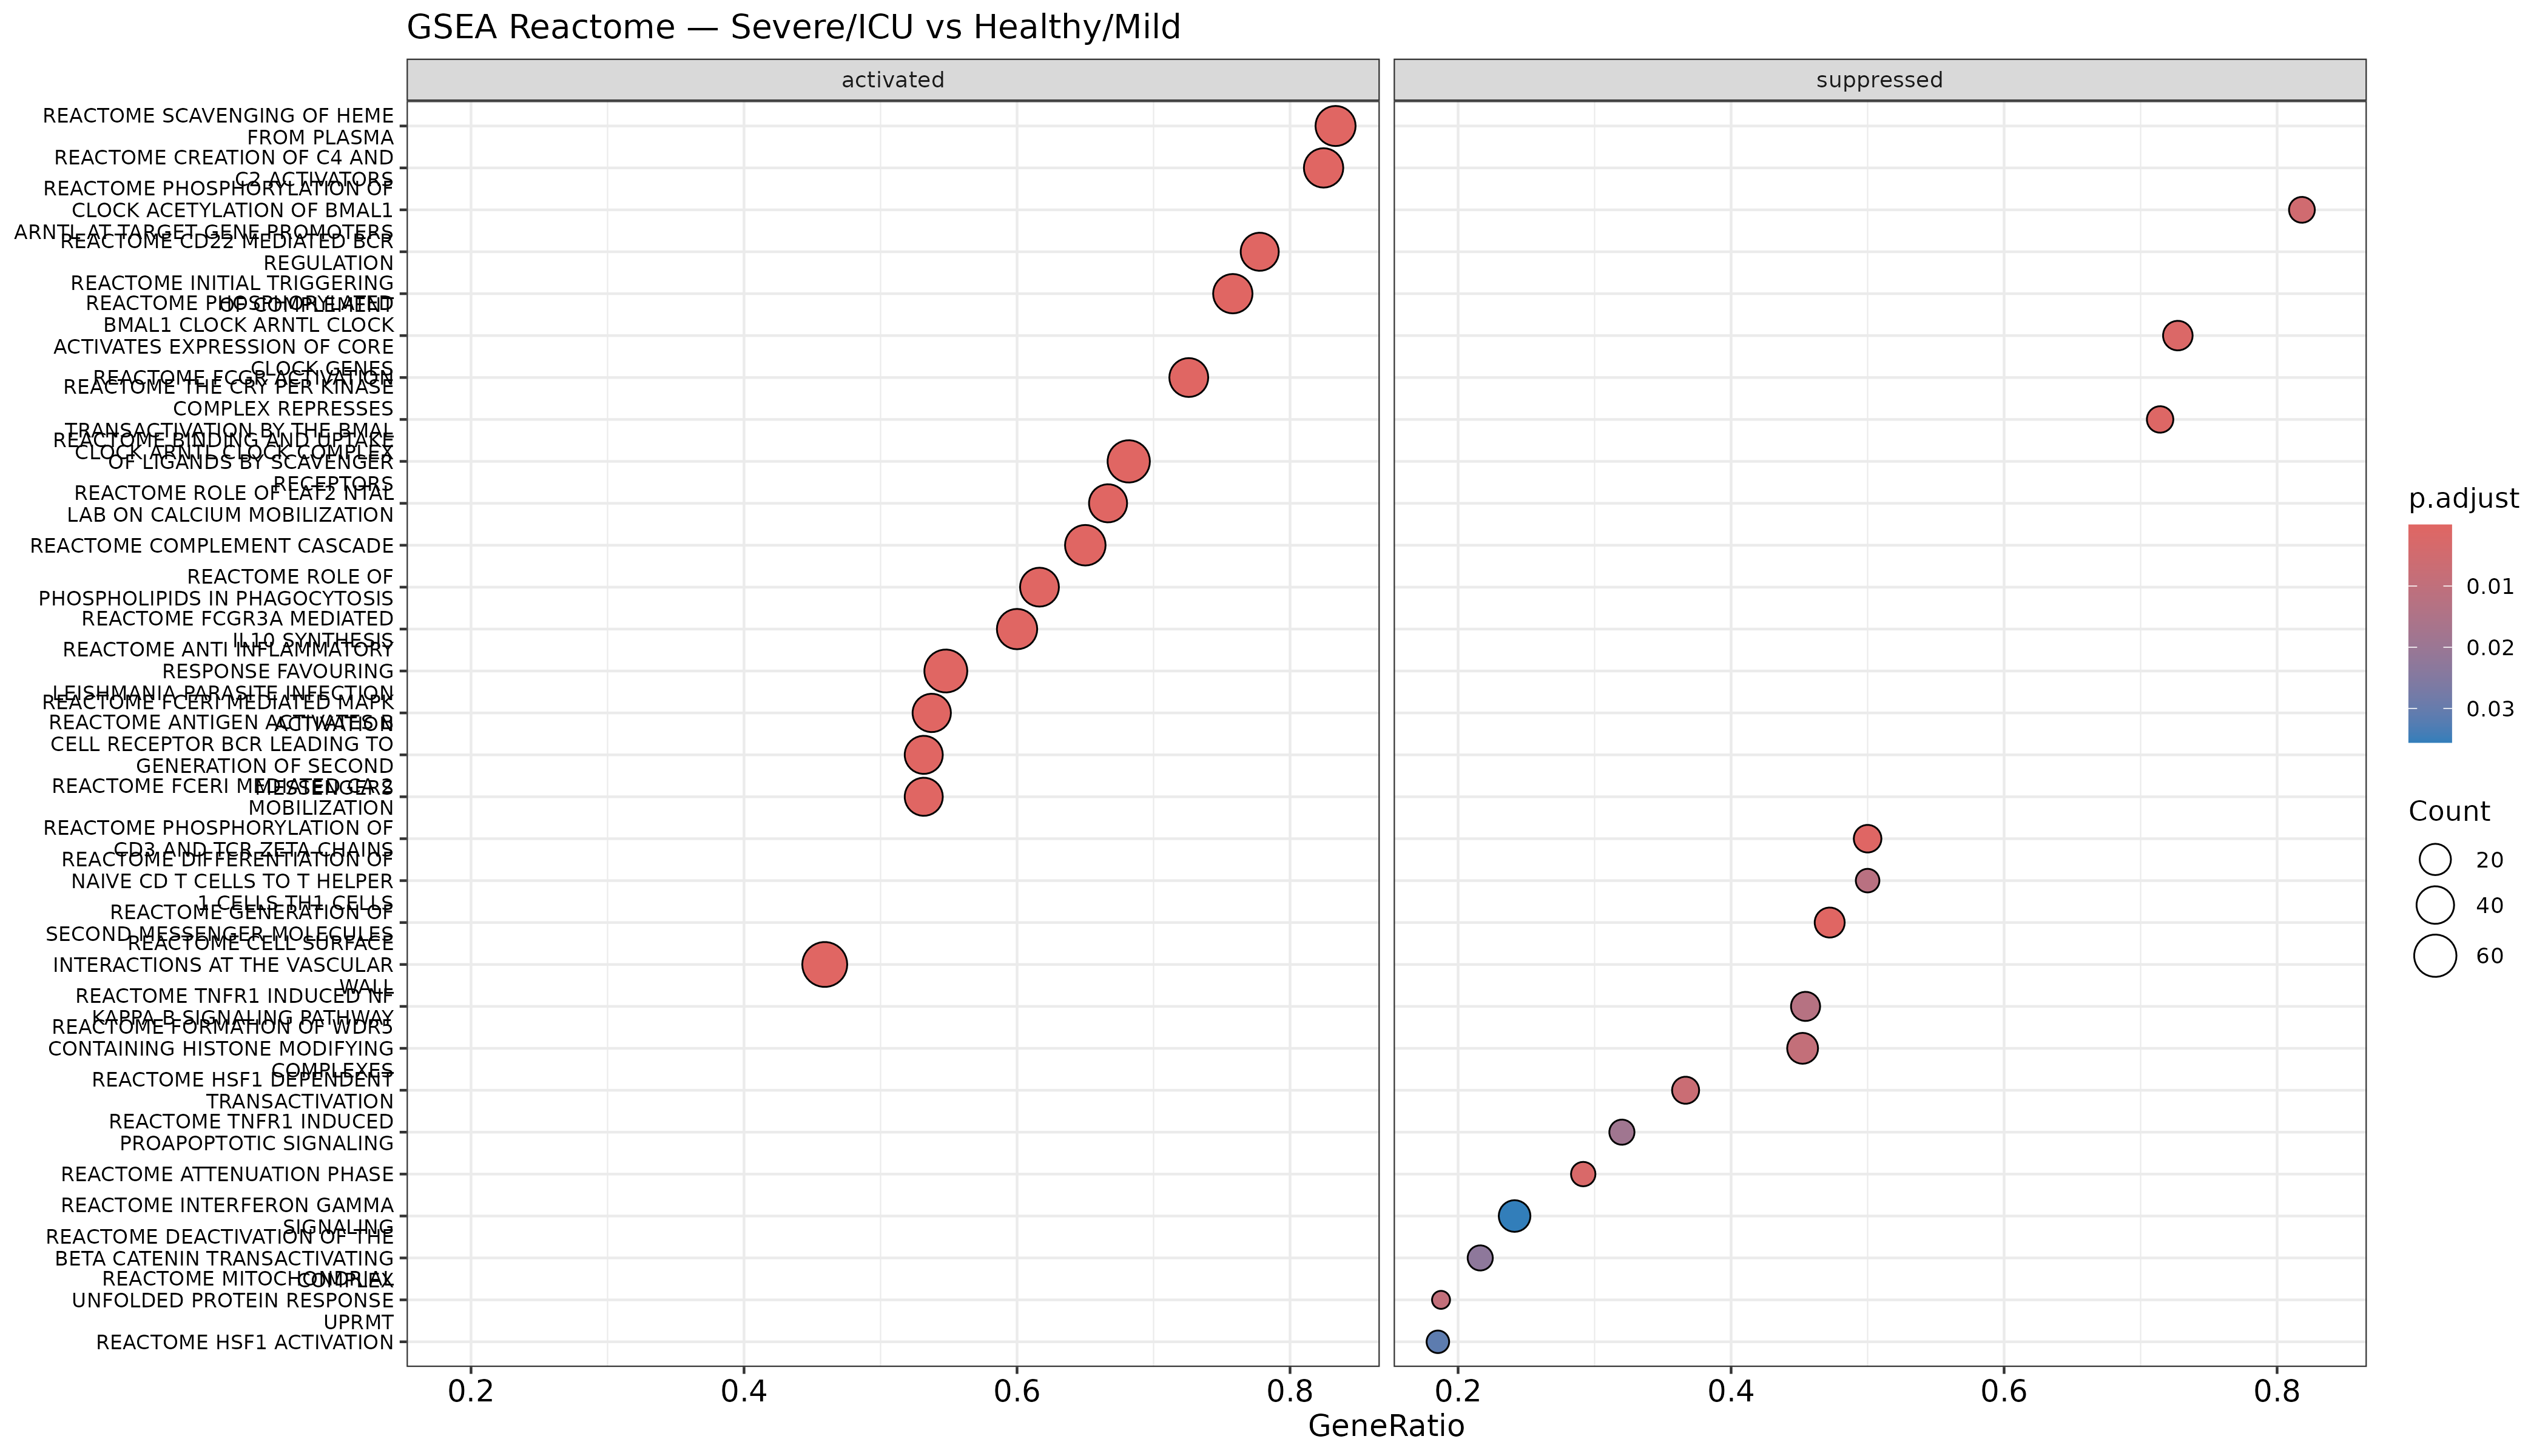
\includegraphics[width=\textwidth]{plots/phase12/phase12_reactome_dotplot.png}
\end{center}

Reactome provides the most detailed molecular-level annotations. Several new
insights emerge that were not visible in the other databases.

\textit{Activated:}
\begin{itemize}[nosep]
  \item \textbf{Scavenging of Heme from Plasma ($\approx$ 0.83)} — the single most
        activated Reactome pathway. Heme scavenging involves hemopexin and haptoglobin,
        proteins released when red blood cells lyse. Its top position confirms that
        hemolysis and RBC breakdown is occurring — consistent with erythrocyte
        contamination in Phase 3 and the erythrocyte development signal in GO:BP.
        In severe COVID, hemolysis is a known complication driven by complement
        attack on RBCs.
  \item \textbf{Creation of C4 and C2 Activators ($\approx$ 0.80) and Initial
        Triggering of Complement ($\approx$ 0.64)} — the lectin and classical
        complement pathways are strongly activated. This aligns with the coagulation
        and complement signal across all three other databases.
  \item \textbf{Complement Cascade ($\approx$ 0.56)} — higher up in the pathway
        hierarchy, confirming the entire complement system is activated in Severe.
  \item \textbf{Interactions at the Vascular Wall ($\approx$ 0.43)} — leukocyte
        adhesion to the endothelium; consistent with platelet activation and
        thrombotic pathology.
\end{itemize}

\textit{Suppressed — the circadian rhythm finding:}
\begin{itemize}[nosep]
  \item \textbf{BMAL1 Clock/ARNTL Target Gene Promoters ($\approx$ 0.82 suppressed
        GeneRatio)} and multiple related circadian clock terms — the most
        significantly suppressed Reactome pathways.
        BMAL1 and CLOCK are the core proteins of the circadian rhythm machinery that
        controls the 24-hour cycle of gene expression in immune cells and throughout
        the body. Their suppression in severe COVID blood is biologically meaningful:
        ICU patients have disrupted light-dark cycles, continuous medical interventions,
        and severe physiological stress. All of these disrupt circadian gene expression.
        Moreover, circadian disruption weakens immune responses and is an independent
        factor in poor outcomes. This is the most novel finding in Phase 12.
  \item \textbf{Reactome Interferon Gamma ($\approx$ 0.25 suppressed)} — IFN-$\gamma$
        is produced by T cells and NK cells, both depleted in Severe. Consistent with
        the KEGG T cell receptor suppression and the lymphopenia from Phase 4.
  \item \textbf{TNFR1-Induced NF-$\kappa$B Signaling} — the TNF-NF-$\kappa$B
        suppression from Hallmark is confirmed here at a more mechanistic level.
\end{itemize}

\subsection{Phase 12 conclusion}

Phase 12 places the individual gene findings from Phase 8 into their full
biological context. The pathway-level picture is:

\begin{enumerate}[nosep]
  \item \textbf{Innate immunity surges.}
        Complement, coagulation, heme scavenging, and antibacterial humoral
        programs are all activated — confirmed independently in GO:BP, Hallmark,
        KEGG, and Reactome. This is the myeloid/platelet expansion captured as
        gene sets instead of individual genes.

  \item \textbf{Adaptive immunity collapses.}
        T cell receptor signaling, CD4$^+$ T cell activation, antigen presentation,
        and lymphocyte differentiation programs are all suppressed.
        The lymphopenia from Phase 4 is confirmed at the pathway level.

  \item \textbf{Cells are proliferating.}
        MYC targets, mTORC1, G2M checkpoint, E2F targets, and cell cycle are
        all activated — the gene signature of actively dividing cells,
        consistent with emergency myelopoiesis.

  \item \textbf{Mitochondrial metabolism is reprogrammed.}
        Oxidative phosphorylation and reactive oxygen species are the
        top activated Hallmark and KEGG programs. Immune cells in severe
        COVID are running on mitochondrial respiration, not the aerobic
        glycolysis typical of activated immune cells.

  \item \textbf{TNF/NF-$\kappa$B is suppressed in bulk blood.}
        The inflammatory program central to the co-activation hypothesis
        appears as a \textit{net loss} at the bulk level (NES negative,
        p $= 10^{-10}$), confirming the Phase 10 finding. The single-cell
        data was necessary to reveal that this suppression is an artefact of
        cell composition, not a true biological suppression.

  \item \textbf{Circadian rhythm is disrupted.}
        The BMAL1/CLOCK gene program is the most suppressed Reactome pathway.
        This novel finding suggests severe COVID patients have wholesale
        disruption of the circadian immune control machinery, which may
        compound disease severity.
\end{enumerate}

\textbf{What this means for the story:}
The bulk gene expression data describes a body in a state of acute crisis:
innate and coagulation systems active, adaptive immune system offline,
cells proliferating to replace losses, and normal circadian regulation abandoned.
Phase 13 will close the loop by returning to the original co-activation question
and asking: if we specifically look for the monocyte co-activation signature
in the bulk data, can we detect it above this background?

% ─────────────────────────────────────────────────────────
\subsection{ssGSEA — scoring one sample at a time}

GSEA (Phase 12) compares \textit{across} a group of samples — it asks
whether a pathway is enriched in Severe \textit{on average}.
\textbf{ssGSEA (single-sample GSEA)} does something different: it gives
\textit{every individual sample} its own enrichment score for a gene set.

For each sample, ssGSEA ranks all genes by expression level and computes
an enrichment score between the signature genes and the rest — similar to
GSEA's running sum, but applied to one sample independently.

\textbf{Why use ssGSEA here?}
It is more sensitive than looking at individual gene counts because it
uses the coordinated signal across all genes in the module simultaneously.
If 17 ISG genes all go slightly up in the same sample, ssGSEA detects
that as a meaningful positive score even if no single ISG gene alone
crosses a significance threshold.

The result is a number between 0 and 1 per sample per module:
a higher score means the sample's transcriptome is more enriched for
that program relative to the background. The question is:
\textit{are Severe/ICU samples enriched for the co-activation signature
even when individual genes were not detectable?}

% ─────────────────────────────────────────────
\section{Phase 13 — Monocyte Co-Activation Signature in Bulk}
% ─────────────────────────────────────────────

\subsection{Phase 13 overview — the big picture}

\textbf{Phases 4--5 found the co-activation signal in single cells.
Phases 7--12 showed it was invisible in bulk individual genes and even in pathway analysis.
Phase 13 is the final test: using the most sensitive bulk method available,
can we detect any trace of the co-activation signature in whole blood?}

The approach:
\begin{enumerate}[nosep]
  \item Build a compact monocyte co-activation signature from the Phase 4
        DE gene lists — the same ISG genes and TNF/IL-1$\beta$ genes used
        to score monocytes in Phase 4.
  \item Score \textit{every bulk sample individually} using ssGSEA.
  \item Visualize the raw expression of signature genes across samples (heatmap).
  \item Compare ISG and TNF/IL-1$\beta$ scores between Healthy/Mild and
        Severe/ICU (boxplots).
  \item Plot ISG score vs TNF/IL-1$\beta$ score as a scatter — the bulk-level
        version of the Phase 4 co-activation scatter.
\end{enumerate}

\textbf{The signature used:}
\begin{itemize}[nosep]
  \item \textbf{ISG module (17 genes):} ISG15, IFIT1, IFIT2, IFIT3, MX1, MX2,
        OAS1, OAS2, OAS3, IFI44L, IFI44, RSAD2, HERC5, HERC6, ISG20, TRIM22, XAF1.
  \item \textbf{TNF/IL-1$\beta$ module (15 genes):} TNF, IL1B, IL6, CXCL8, CCL3,
        CCL4, CCL2, CXCL10, PTGS2, S100A8, S100A9, NLRP3, CASP1, IL18, IL8.
\end{itemize}

\subsection{Signature heatmap \small\normalfont\textit{(Step 5)}}

\begin{center}
  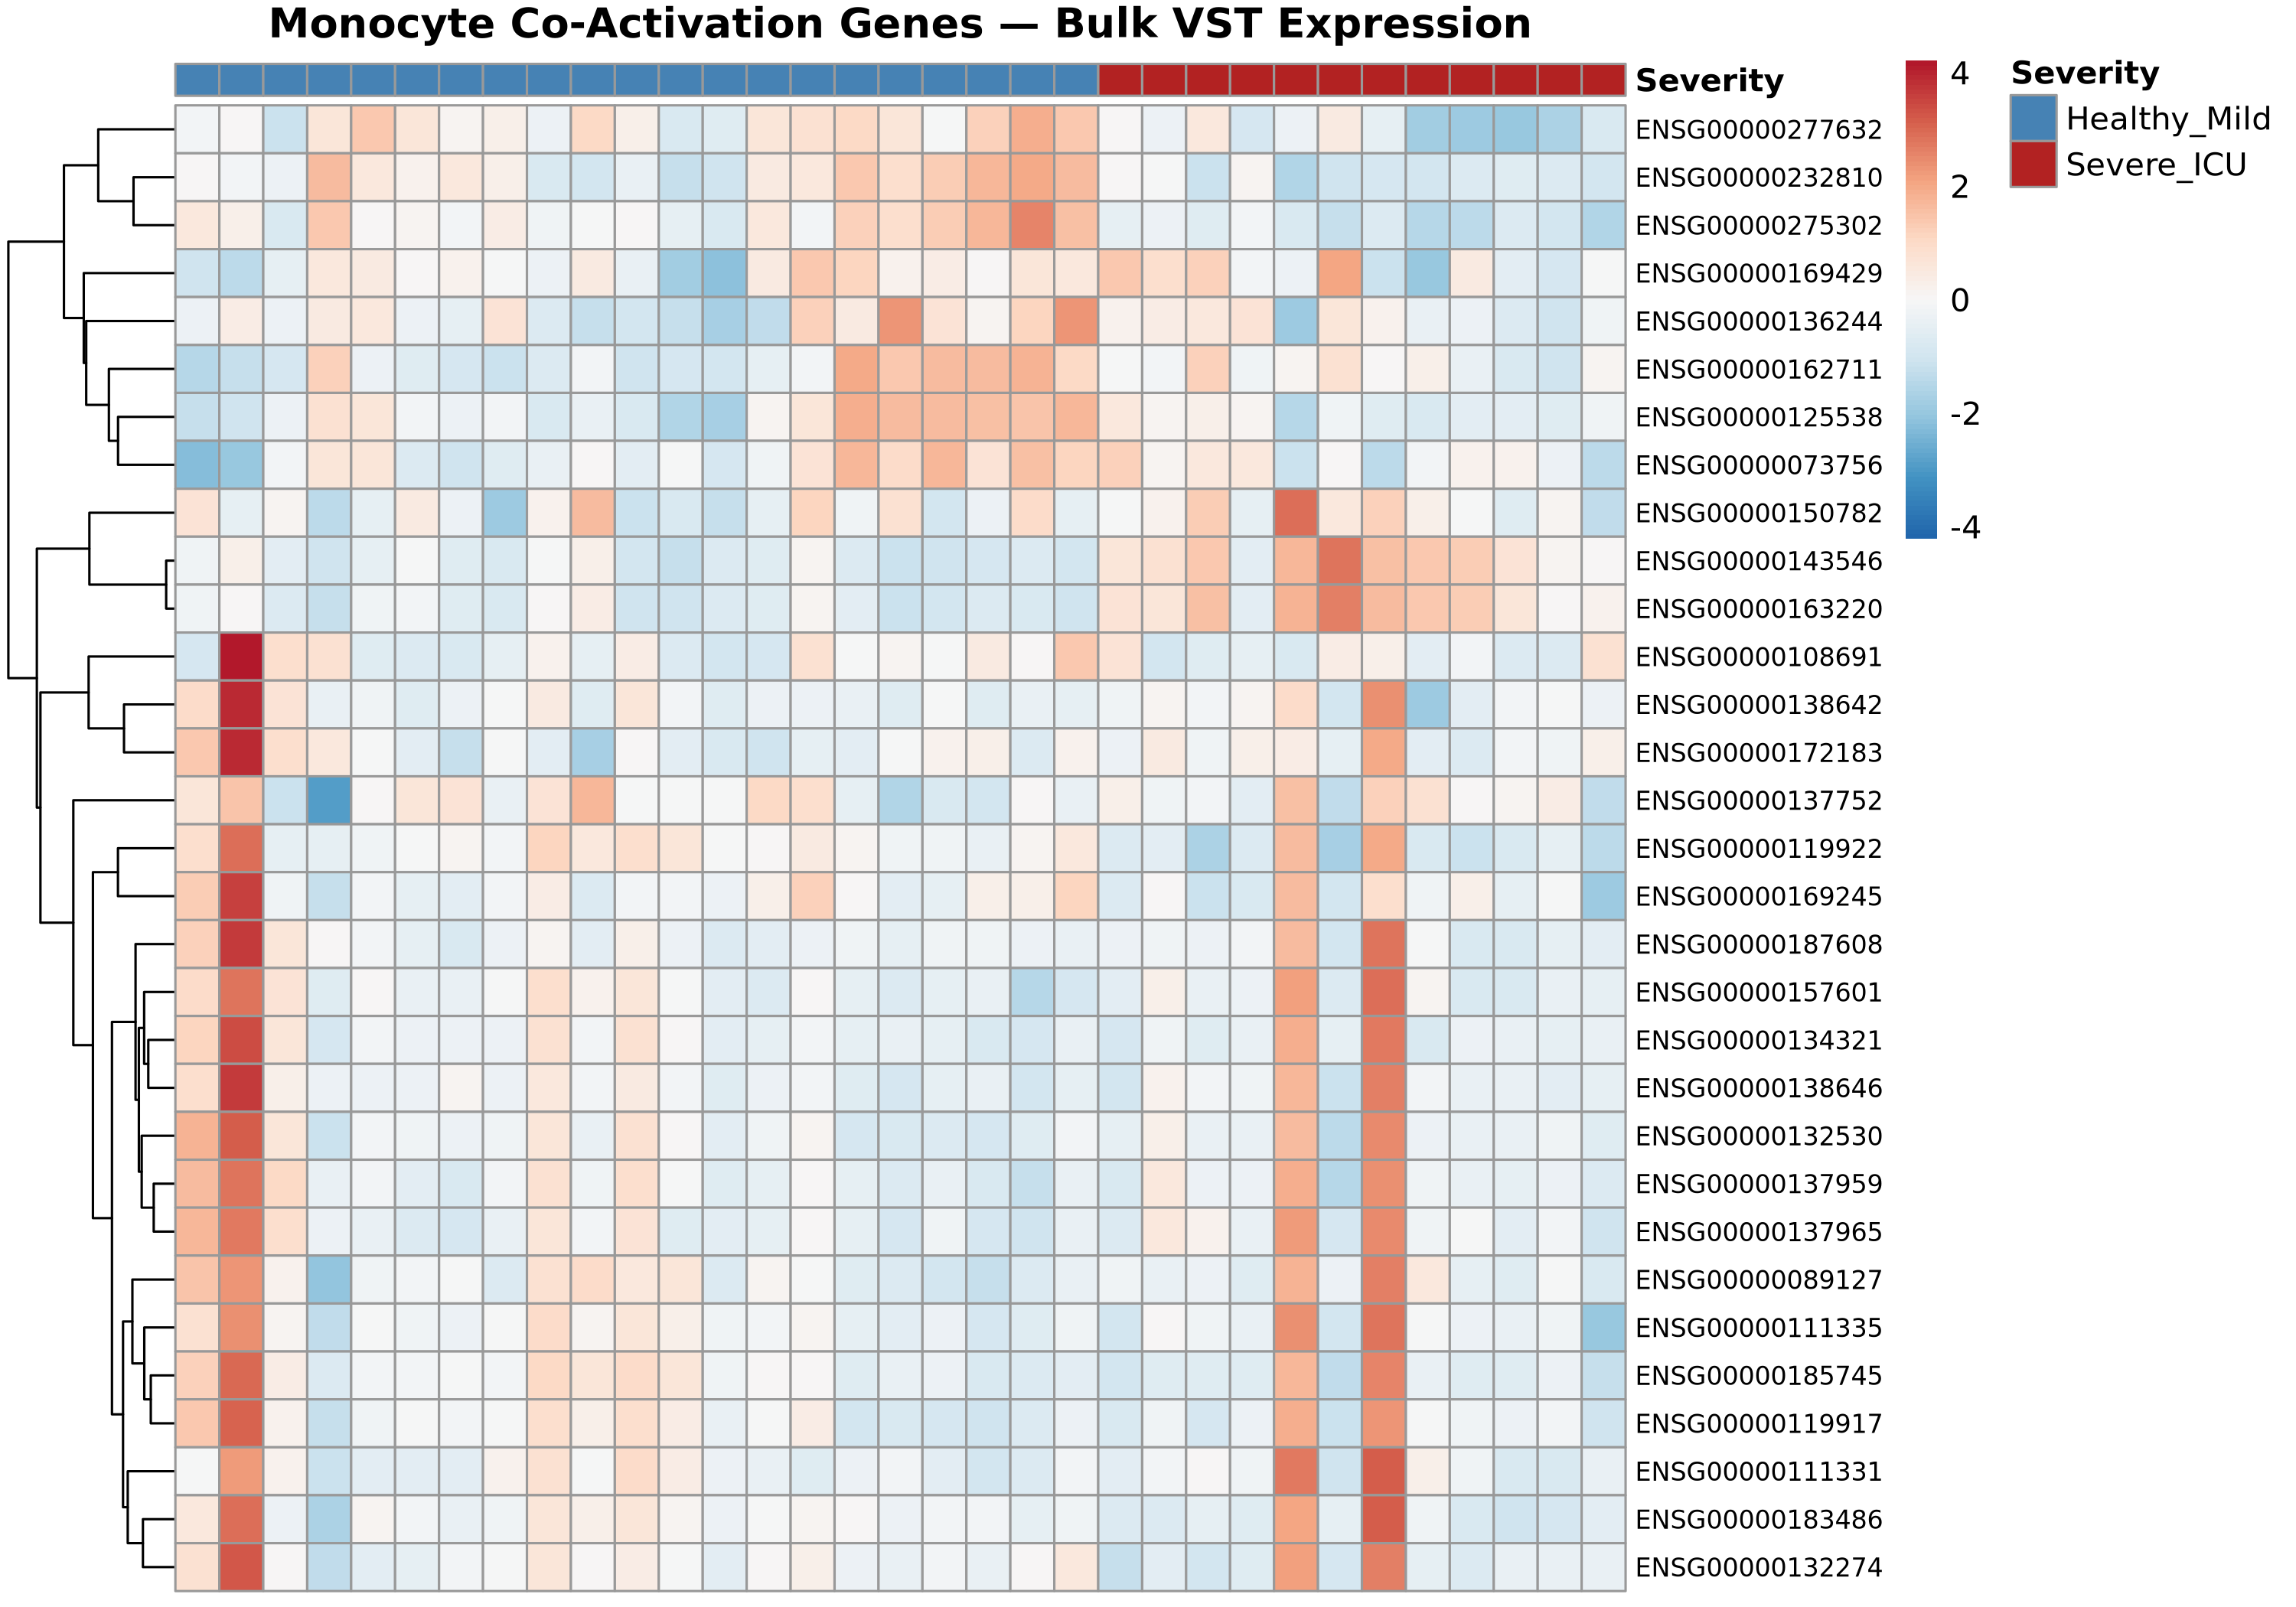
\includegraphics[width=\textwidth]{plots/phase13/phase13_signature_heatmap.png}
\end{center}

The heatmap shows the VST-normalized expression of all 32 co-activation
signature genes across all 33 bulk samples. Row labels are Ensembl IDs
(because the bulk count matrix uses Ensembl identifiers rather than gene symbols).
Columns are ordered with Healthy/Mild on the left and Severe/ICU on the right
(annotation bar at top). Colour: red = high expression; blue = low; white = average.

\begin{itemize}[nosep]
  \item \textbf{No clean severity-driven block structure.}
        Unlike the Phase 8/10 heatmaps — where the top 30--50 DE genes separated
        groups with a nearly perfect two-block pattern — the co-activation signature
        genes show a \textbf{mixed, noisy pattern}. There is no block of genes
        consistently red in Severe and blue in Healthy, or vice versa.
  \item \textbf{Individual-sample variability dominates.}
        Several single columns light up brightly for specific genes — individual
        donors with unusually high expression of one or a few ISG or TNF genes.
        These isolated bright spots do not form a coherent group signal.
  \item \textbf{Within-Healthy variability is comparable to within-Severe variability.}
        Looking at the Healthy/Mild columns, the pattern is just as heterogeneous
        as the Severe/ICU side. This is the visual equivalent of what the Phase 10
        boxplots showed numerically: these genes are variable in \textit{all} groups.
  \item \textbf{One outlier column} (far left of the Severe block, with a dark red
        cell for one gene) corresponds to the high-expression donor seen in the
        Phase 10 ISG15 boxplot. A single donor with unusually elevated expression
        of one ISG gene does not constitute group-level enrichment.
\end{itemize}

\textbf{Interpretation:} the co-activation signature genes do not show a coordinated
group-level shift in bulk blood. Their expression is donor-variable and scattered.
The more sensitive ssGSEA scoring in the next step will test whether any aggregate
signal exists despite this noise.

\subsection{Module score boxplots \small\normalfont\textit{(Step 6)}}

\begin{center}
  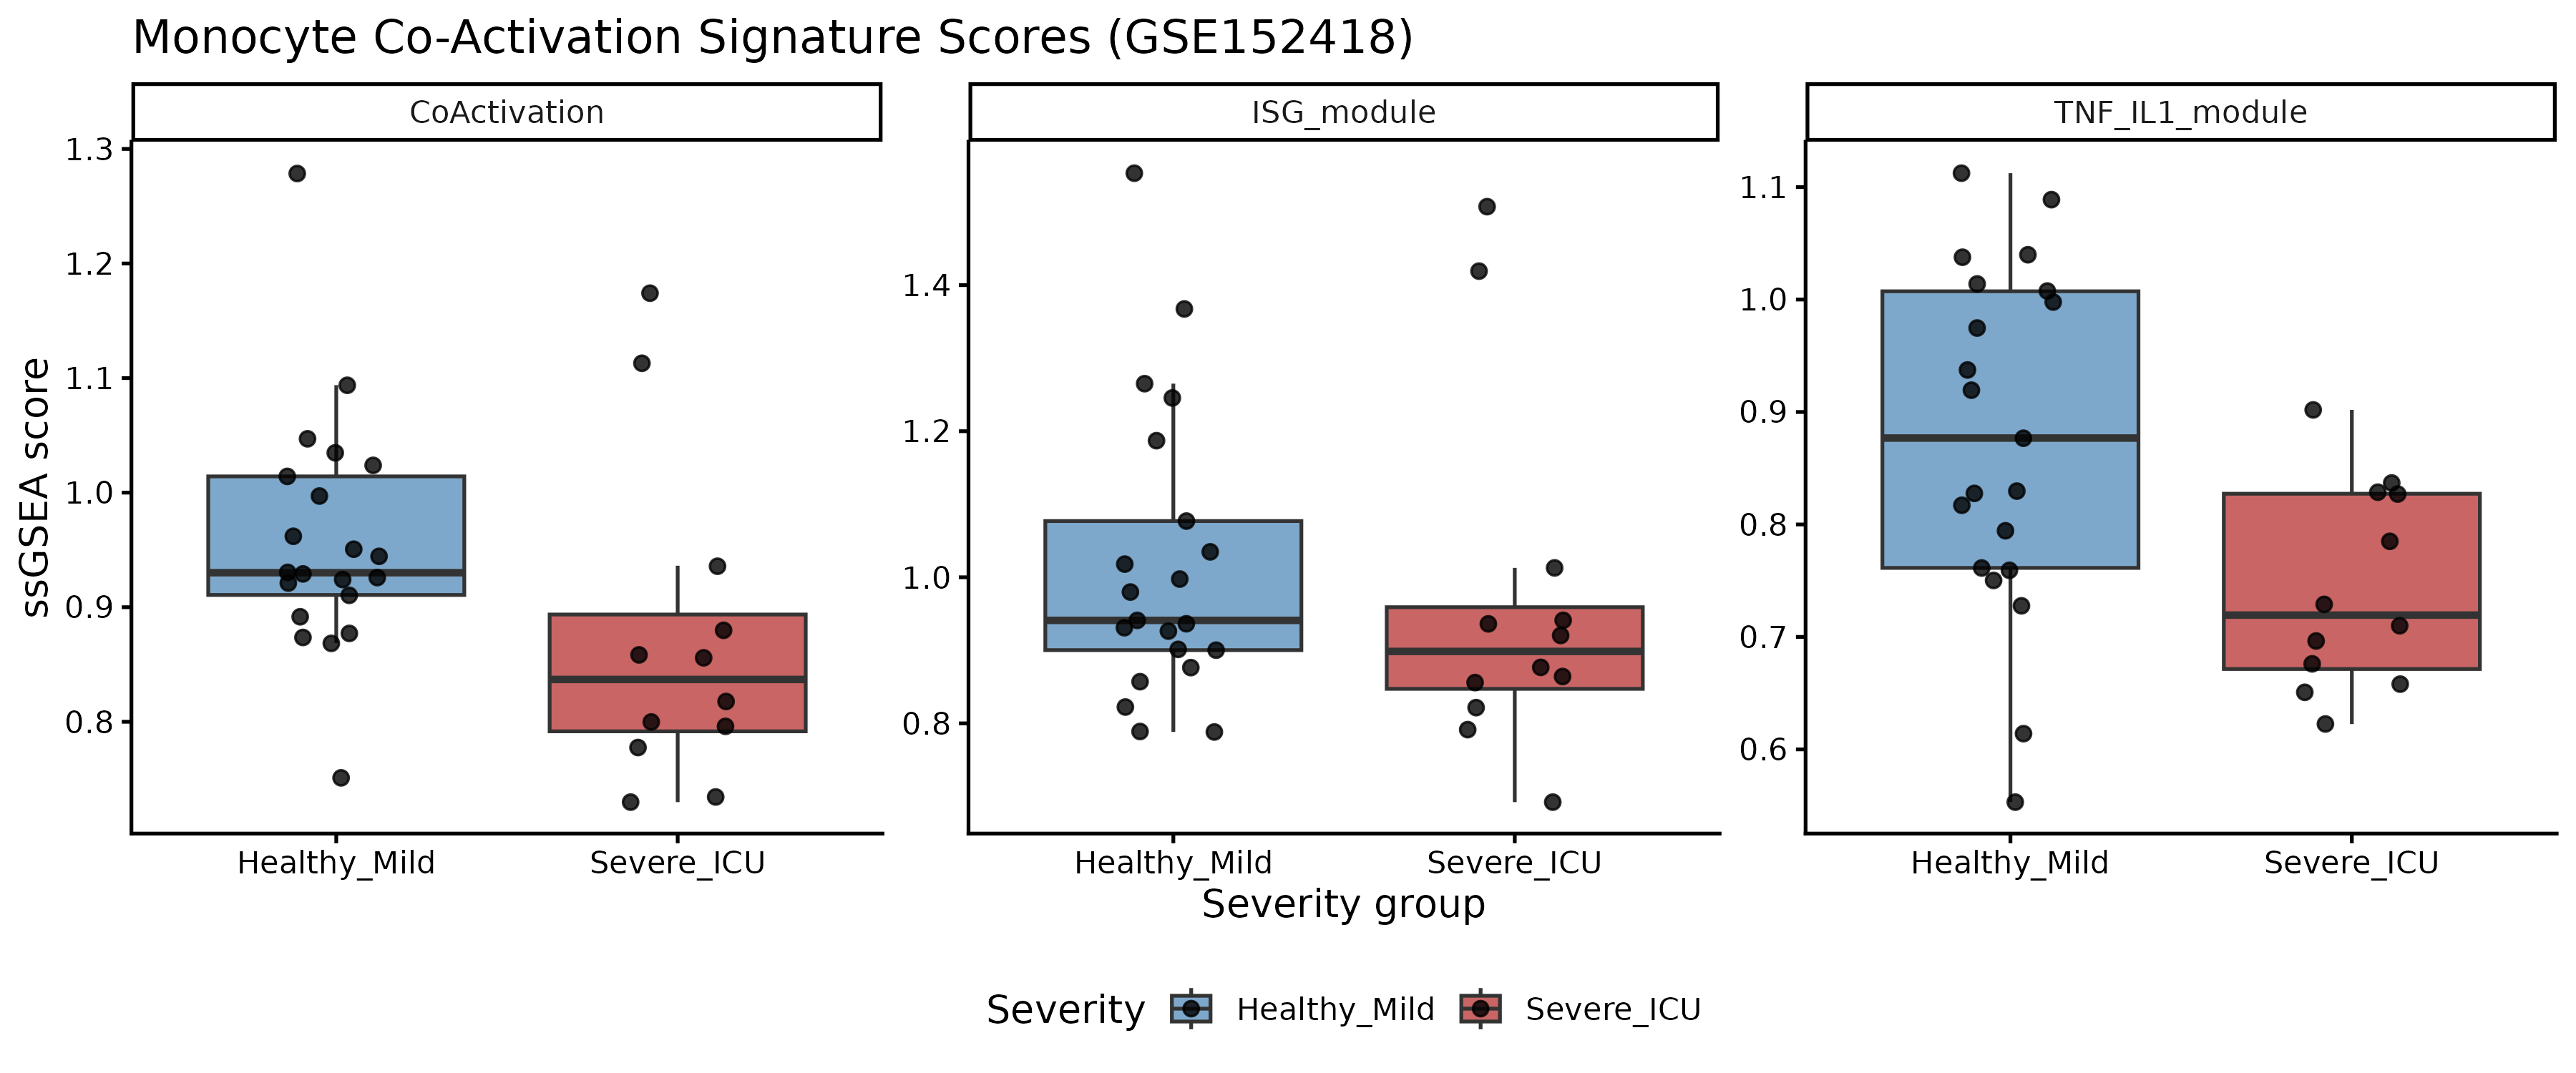
\includegraphics[width=\textwidth]{plots/phase13/phase13_score_boxplots_GSE152418.png}
\end{center}

Three boxplots show the ssGSEA score for each module in each sample,
grouped by severity. Each dot is one donor. Y-axis = ssGSEA score (normalized,
higher = more enriched for the program).

\textit{Left — Co-Activation score (combined ISG + TNF/IL-1$\beta$):}
\begin{itemize}[nosep]
  \item \textbf{Healthy/Mild} median $\approx$ 0.95; most donors between 0.88 and 1.00.
  \item \textbf{Severe/ICU} median $\approx$ 0.84; most donors between 0.78 and 0.92.
  \item The Severe/ICU box sits \textbf{lower}, not higher.
        The combined co-activation signature is \textit{less} enriched in Severe blood.
\end{itemize}

\textit{Middle — ISG module score:}
\begin{itemize}[nosep]
  \item \textbf{Healthy/Mild} median $\approx$ 0.97; a broad spread from 0.82 to 1.28.
  \item \textbf{Severe/ICU} median $\approx$ 0.91; spread from 0.78 to 1.24.
  \item Again, Severe/ICU is slightly \textbf{lower}. One Healthy/Mild outlier reaches
        1.45 (the same high-ISG donor seen throughout the bulk chapter). With this
        outlier, the Healthy group median is pulled up further.
\end{itemize}

\textit{Right — TNF/IL-1$\beta$ module score:}
\begin{itemize}[nosep]
  \item \textbf{Healthy/Mild} median $\approx$ 0.88; tight cluster from 0.63 to 1.05.
  \item \textbf{Severe/ICU} median $\approx$ 0.72; spread from 0.60 to 1.10.
  \item \textbf{The most dramatic separation:} the Severe/ICU box is clearly below
        the Healthy/Mild box. The TNF/IL-1$\beta$ program is \textit{less} enriched
        in Severe COVID whole blood — the same direction as all the Phase 10 boxplots
        and the Phase 12 TNF/NF-$\kappa$B GSEA result.
\end{itemize}

\textbf{The same paradox, confirmed by a third independent method.}
After looking at individual gene counts (Phase 10), pathway-level GSEA (Phase 12),
and now ssGSEA module scores (Phase 13), the answer is always the same:
the monocyte co-activation programs are not elevated in Severe COVID whole blood.
They are, if anything, slightly lower.

\subsection{Co-activation scatter — the bulk version \small\normalfont\textit{(Step 7)}}

\begin{center}
  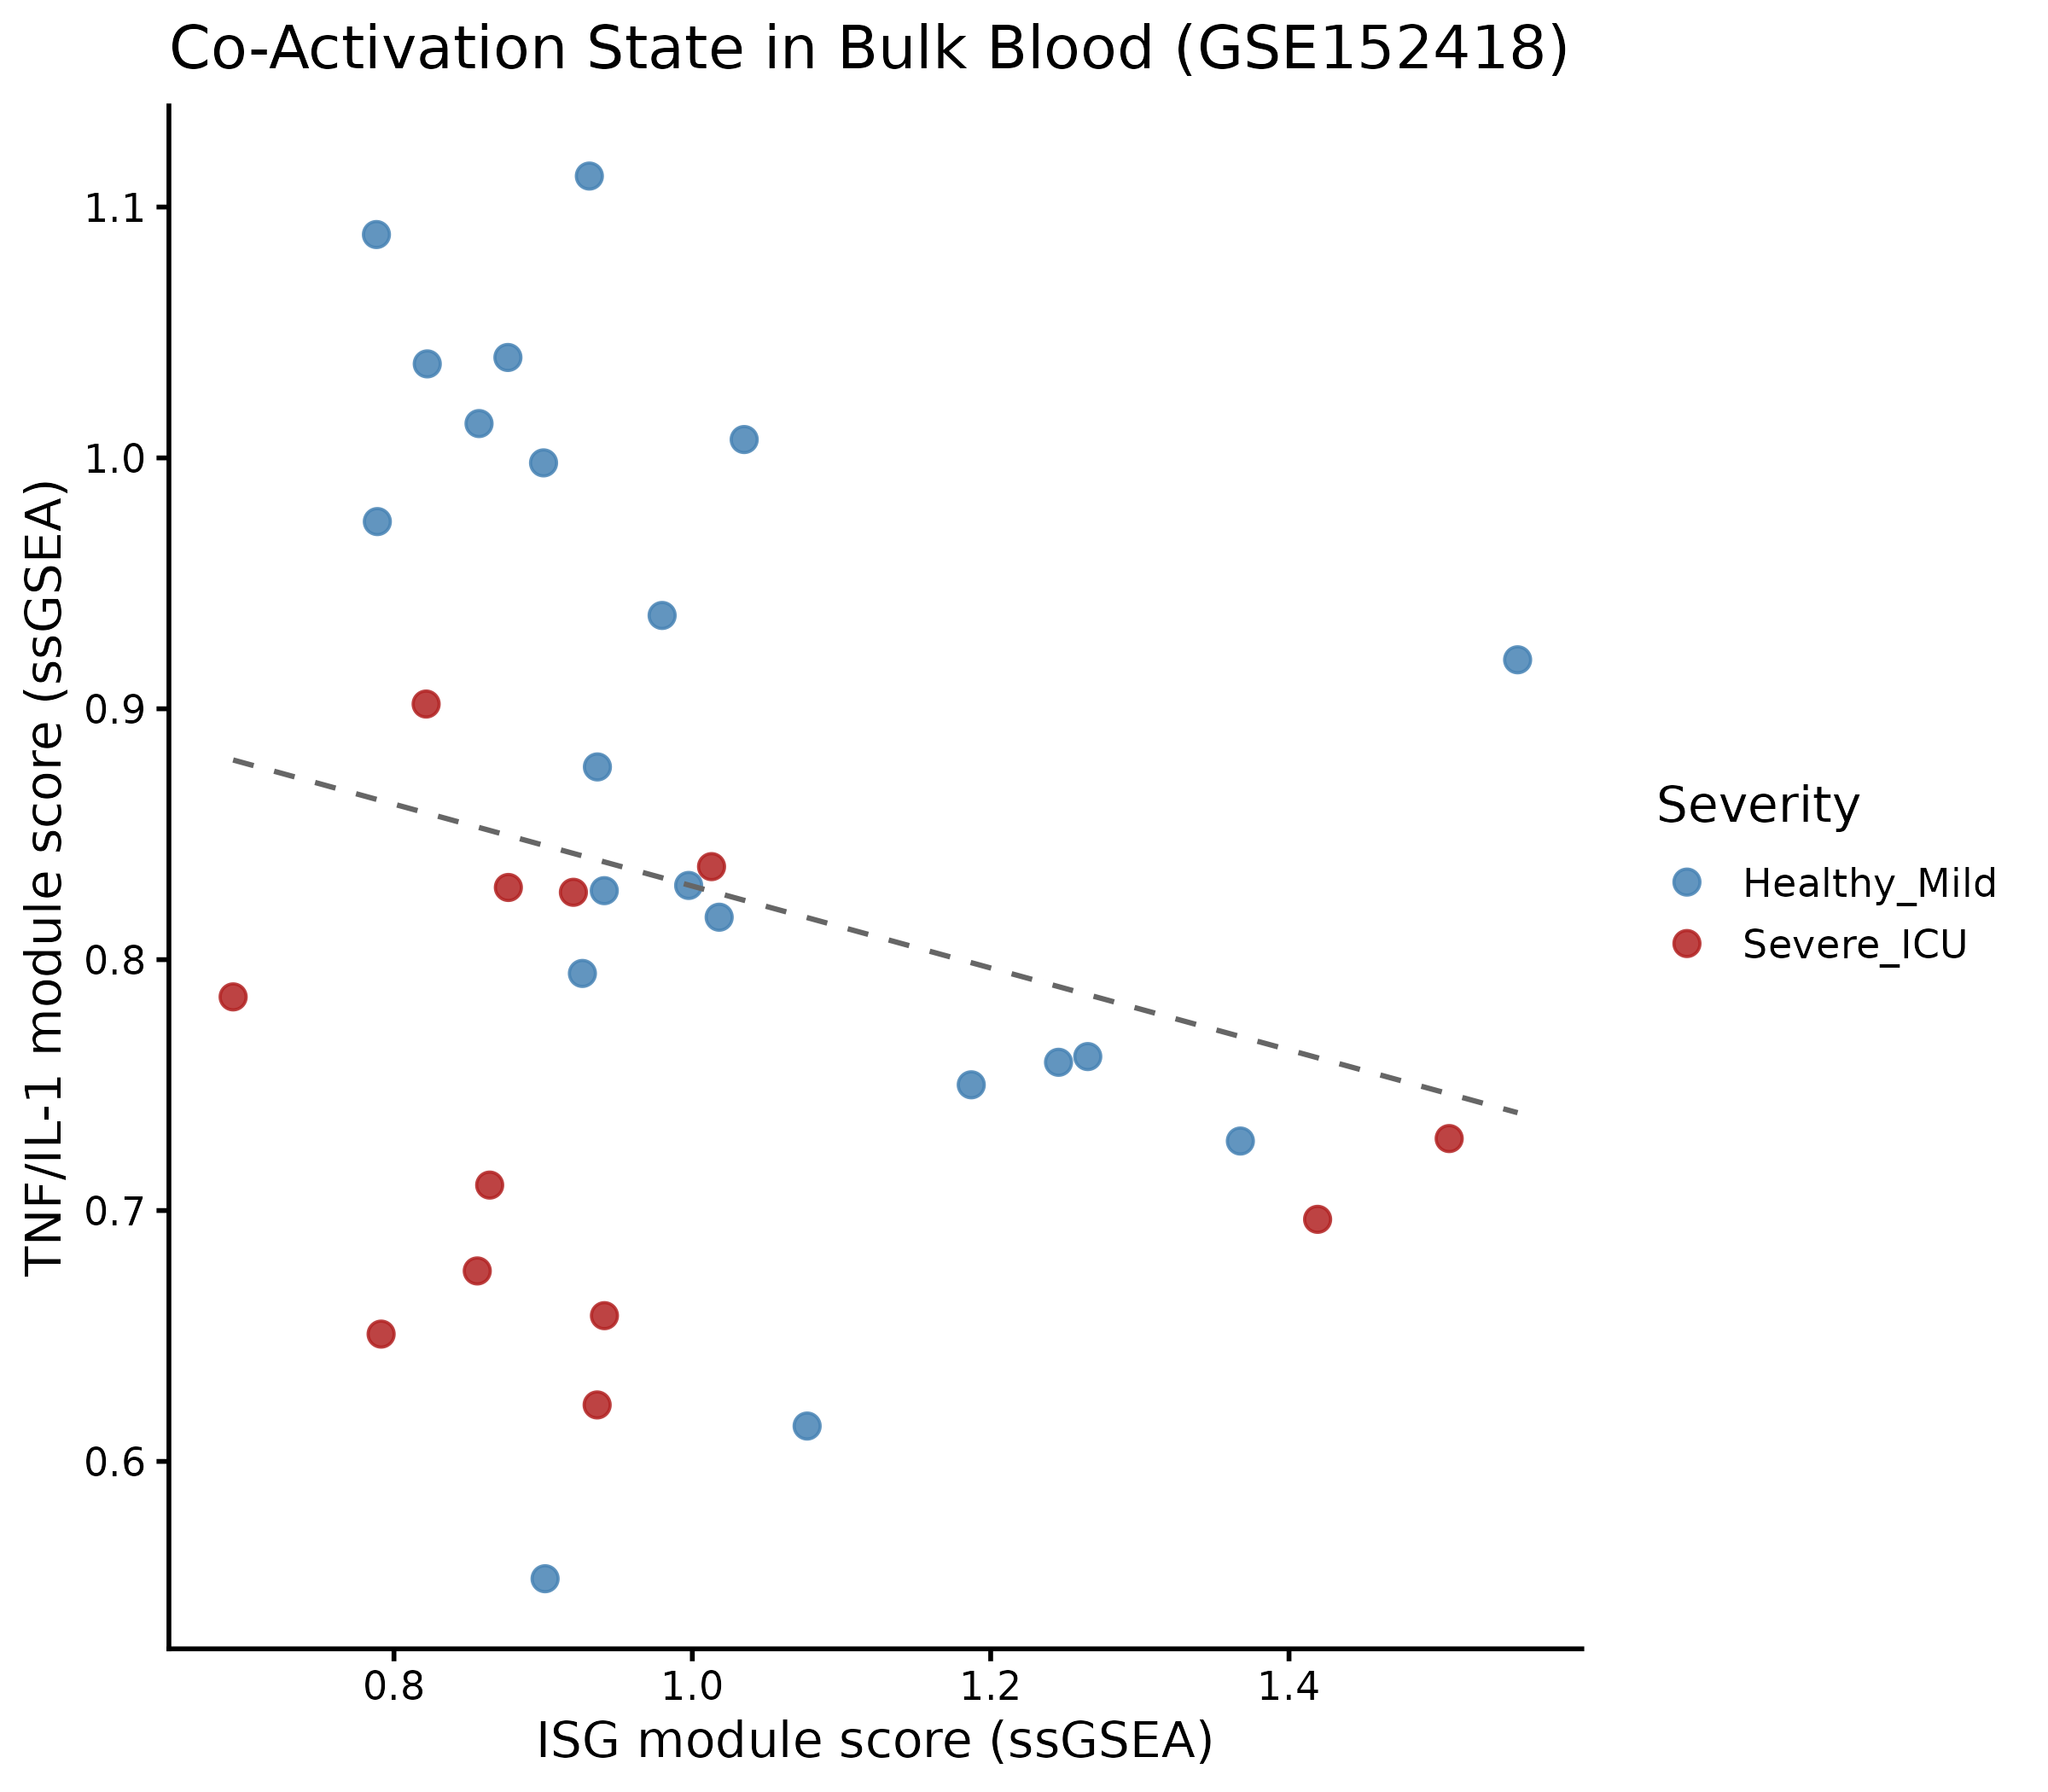
\includegraphics[width=0.85\textwidth]{plots/phase13/phase13_coactivation_scatter_GSE152418.png}
\end{center}

This is the bulk-level version of the central Phase 4 co-activation scatter.
Each dot is one \textit{whole blood sample} (not a single monocyte).
x-axis = ISG module ssGSEA score; y-axis = TNF/IL-1$\beta$ module ssGSEA score.
Blue = Healthy/Mild; red = Severe/ICU. The dashed line is the linear trend.

\begin{itemize}[nosep]
  \item \textbf{Healthy/Mild samples (blue) occupy the upper half of the plot.}
        Most blue dots sit above y $\approx$ 0.82, with many reaching 0.95--1.11.
        They are distributed across a wide range of ISG scores (x $\approx$ 0.82--1.52)
        but maintain high TNF/IL-1$\beta$ scores.

  \item \textbf{Severe/ICU samples (red) occupy the lower half.}
        Nearly all red dots are below y $\approx$ 0.90, and most are below 0.85.
        They cluster in the lower-left and lower-right areas.
        There are \textbf{no red dots in the upper-right} (high ISG \textit{and}
        high TNF/IL-1$\beta$) — the co-activated quadrant that was the focus
        of the single-cell analysis is \textbf{empty of Severe samples}.

  \item \textbf{The trend line has a negative slope.}
        Higher ISG score correlates weakly with \textit{lower} TNF/IL-1$\beta$
        score across all samples. The two programs do not co-activate in bulk
        blood — they show a slight inverse relationship.
        This is the opposite of co-activation, and it reflects the compositional
        reality: the samples with the most ISG signal are those with the most
        surviving lymphocytes (which also produce ISG), and lymphocyte-rich samples
        are by definition \textit{not} the Severe samples with expanded monocytes.

  \item \textbf{Compare to Phase 4:} in the single-cell monocyte scatter, Severe
        samples pushed cells into the top-left (high TNF/IL-1$\beta$, low ISG)
        and some into the top-right co-activated quadrant. In this bulk scatter,
        Severe samples move to the \textit{bottom} — they lose both signals.
\end{itemize}

\subsection{Phase 13 conclusion — and the final answer}

Phase 13 applies the most sensitive bulk detection method available
(ssGSEA scoring with the exact same Phase 4 gene lists) and reaches the same
conclusion as Phases 10 and 12:

\begin{enumerate}[nosep]
  \item \textbf{The co-activation signature is not enriched in Severe/ICU
        bulk blood.} All three modules (ISG, TNF/IL-1$\beta$, combined) score
        \textit{lower} in Severe/ICU than in Healthy/Mild.

  \item \textbf{The bulk co-activation scatter is the mirror image of the
        single-cell scatter.} In Phase 4, Severe monocytes moved toward
        high TNF/IL-1$\beta$. In Phase 13, Severe blood samples move toward
        low TNF/IL-1$\beta$. The two findings are not contradictory — they
        are caused by the same mechanism: the lymphocyte depletion that
        accompanies monocyte expansion removes a large constitutive source
        of these transcripts from the bulk mix.

  \item \textbf{Three independent bulk methods agree.}
        Individual gene counts (Phase 10), pathway GSEA (Phase 12), and
        ssGSEA module scoring (Phase 13) all point in the same direction.
        The co-activation signal is genuinely invisible in whole blood.

  \item \textbf{Single-cell RNA-seq was necessary.}
        The co-activated monocyte state is real — confirmed in two independent
        scRNA-seq cohorts (Phase 4 and Phase 5) and reversible by Tocilizumab.
        But it is a property of a small subset of cells within an already
        minority cell type. That signal cannot survive the averaging that
        bulk RNA-seq performs across all cell types and all monocyte sub-states.
\end{enumerate}

\subsection{Overall project conclusion}

The full story is now complete. Assembling all phases together:

\begin{description}[leftmargin=0pt, itemsep=6pt]
  \item[\normalfont\textbf{Phases 1--3} \textit{(scRNA-seq foundation)}]
    A high-quality single-cell dataset of 55,548 PBMC cells was built, normalized,
    and annotated. Ten monocyte sub-clusters were identified, several of which
    carry strong COVID-relevant biology: ISG-high (Cluster 10), IL-1$\beta^+$
    inflammasome-active (Cluster 7), and chemokine-secreting (Cluster 18).
    The blood immune landscape was already dramatically altered at the cell-type level.

  \item[\normalfont\textbf{Phases 4--5} \textit{(co-activation discovery and replication)}]
    Monocytes expand with severity while T cells deplete. A subset of monocytes
    simultaneously activates both the antiviral (ISG) and inflammatory (TNF/IL-1$\beta$)
    programs — the co-activated state. This state replicated in an independent
    dataset (GSE150861) and was suppressed by Tocilizumab within 4 days.

  \item[\normalfont\textbf{Phase 6} \textit{(scRNA-seq visual summary)}]
    The single-cell chapter was assembled into a clean, publication-quality figure set.
    The key summary: Mild COVID = ISG-dominant monocytes; Severe COVID = TNF/IL-1$\beta$-dominant monocytes.
    The two programs diverge, not converge, as disease worsens.

  \item[\normalfont\textbf{Phases 7--9} \textit{(bulk data, EDA, and robustness)}]
    Bulk RNA-seq from 33 whole-blood samples (GSE152418) was loaded, cleaned,
    and tested for DE with DESeq2. Gender imbalance was flagged and corrected;
    the results held with $r = 0.97$ between the two models.

  \item[\normalfont\textbf{Phases 10--12} \textit{(bulk signal characterization)}]
    The dominant bulk signal is \textit{not} the monocyte co-activation programs.
    It is the cell composition shift: myeloid/platelet expansion upward,
    lymphocyte depletion downward. The monocyte-specific programs (ISG, TNF/IL-1$\beta$)
    are diluted or net-reduced at the bulk level, confirmed by individual genes,
    GSEA pathways, and the TNF/NF-$\kappa$B enrichment plot.

  \item[\normalfont\textbf{Phase 11} \textit{(unsupervised validation)}]
    Sample-level PCA, correlation, and clustering confirmed the DE findings without
    any label input. PC1 (38\% of variance) separates severity groups with zero
    overlap; k-means and hierarchical clustering recover 97\% accuracy.

  \item[\normalfont\textbf{Phase 13} \textit{(final signature test)}]
    ssGSEA with the exact Phase 4 gene lists fails to detect co-activation
    enrichment in bulk blood. The bulk scatter mirrors Phase 4 in reverse:
    Severe samples are \textit{lower} on both modules.
    Single-cell resolution was indispensable.
\end{description}

\bigskip
\noindent\textbf{The answer to the research question:}

\begin{quote}
\textit{Yes — severe COVID-19 is associated with a classical monocyte state that
shows simultaneous ISG and TNF/IL-1$\beta$ co-activation. This state is real,
reproduced in an independent cohort, and suppressed by Tocilizumab. However,
it is a \textbf{cell-type-specific minority signal} that is completely masked
in whole-blood bulk RNA-seq by the dominant composition shift (myeloid expansion,
lymphocyte depletion). Detecting it required single-cell resolution.}
\end{quote}

\end{document}
